

\documentclass[12pt,a4paper]{book}

\usepackage[margin=8mm]{geometry}
\PassOptionsToPackage{defaults=hu-min,classmod=unchanged}{magyar.ldf}
\usepackage[magyar]{babel}
\usepackage{tikz,pgfplots}

%\documentclass{article}
\usepackage[utf8]{inputenc}
\usepackage{t1enc}
\usepackage[T1,T2A]{fontenc}
\usepackage{graphicx}
\usepackage{multirow}
\usepackage{natbib}
\usepackage{graphicx}
\usepackage{fancyhdr}
\usepackage{mathptmx}
\usepackage{geometry}
\usepackage{ifthen}
\usepackage{enumitem}
\usepackage{float}
\usepackage{capt-of}
\usepackage[section]{placeins}
\usepackage{dblfnote}
\usepackage{nomencl}
\usepackage{amsmath}
\usepackage{pgfplots}
\usepackage{graphicx}
\usepackage{epstopdf}
\usepackage{epsfig}
\usepackage{hyperref}
\usepackage{tikz}
\usepackage{filecontents}
\usetikzlibrary{shapes,arrows,positioning,calc}
\usepackage{amssymb}
\usepackage{gensymb}
\usepackage{datatool, filecontents}
\usepackage{svg}
%\usepackage{luacode}
\usepackage{multirow}
\usepackage{listings}
\usepackage{lipsum}
\usepackage{pgfplotstable, booktabs}
\usepackage{datatool,fp}
\usepackage{color}
\usepackage{amsfonts}
\usepackage[colorinlistoftodos]{todonotes}
\usepackage{algorithm}
\usepackage{algpseudocode}
\usepackage{blindtext}
\usepackage{titlesec}
%\usepackage[svgnames]{xcolor}
%\usepackage{newtxtext,newtxmath}
\usepackage{etoolbox}



\makeatletter
% \patchcmd{<cmd>}{<search>}{<replace>}{<success>}{<failure>}
\patchcmd{\@makechapterhead}{\huge}{\large}{}{}% for \chapter
\patchcmd{\@makechapterhead}{\Huge}{\large}{}{}% for \chapter
\patchcmd{\@makeschapterhead}{\Huge}{\large}{}{}% for \chapter*
\makeatother


%----------------------------XML stilus
\definecolor{gray}{rgb}{0.4,0.4,0.4}
\definecolor{darkblue}{rgb}{0.0,0.0,0.6}
\definecolor{cyan}{rgb}{0.0,0.6,0.6}

\lstset{
  basicstyle=\ttfamily,
  columns=fullflexible,
  showstringspaces=false,
  commentstyle=\color{gray}\upshape
}

\lstdefinelanguage{XML}
{
  morestring=[b]",
  morestring=[s]{>}{<},
  morecomment=[s]{<?}{?>},
  stringstyle=\color{black},
  identifierstyle=\color{darkblue},
  keywordstyle=\color{cyan},
  morekeywords={xmlns,version,type}% list your attributes here
}

% From egreg at https://tex.stackexchange.com/questions/335483/retrieving-substring-of-dtlfetch
\newcommand{\DTLfetchsave}[5]{%
  \edtlgetrowforvalue{#2}{\dtlcolumnindex{#2}{#3}}{#4}%
  \dtlgetentryfromcurrentrow{\dtlcurrentvalue}{\dtlcolumnindex{#2}{#5}}%
  \let#1\dtlcurrentvalue
}


\usetikzlibrary{pgfplots.groupplots, matrix}
\usepgfplotslibrary{groupplots}
\pgfplotsset{%
    compat=1.12,
    minor grid style={dashed,red},
    major grid style={dotted,green!50!black},
    select coords between index/.style 2 args={
    x filter/.code={
        \ifnum\coordindex<#1\def\pgfmathresult{}\fi
        \ifnum\coordindex>#2\def\pgfmathresult{}\fi
    }
}}
\usepackage{subfig}
\captionsetup[subfigure]{labelfont={it,bf},textfont={it,bf},labelformat=parens,labelsep=space}
\usepackage{siunitx}
\usepackage{listings}



\tikzset{
block/.style = {draw, fill=white, rectangle, minimum height=3em, minimum width=3em},
tmp/.style  = {coordinate}, 
sum/.style= {draw, fill=white, circle, node distance=1cm},
input/.style = {coordinate},
output/.style= {coordinate},
pinstyle/.style = {pin edge={to-,thin,black}
}}

\newenvironment{kep}
{   \begin{center}

    \end{center}
}



\title{Kűltéri mobilis robot}								
\author{Gábor Szabolcs László}							
\date{20 Nov 2018}	

\makeatletter
\let\thetitle\@title
\let\theauthor\@author
\let\thedate\@date
\makeatother

\pagestyle{fancy}
\fancyhf{}
%\rhead{Share\LaTeX}
%\lhead{Guides and tutorials}
\rfoot{\center \thepage}

 \geometry{
 a4paper,
 total={170mm,257mm},
 left=25mm,
 right=25mm,
 top=20mm,
 bottom=25mm,
 headheight=15mm
 }
 
%%Formating figure cross references 
\makeatletter
\renewcommand\p@figure{ábra \thesection.\arabic{figure}\expandafter\@gobble}
\makeatother
 
\def\mand#1#2{#1#2} % "macro and"
 
\newcommand\xname{*}
\newcommand\x{*}
\newcommand\y{*}
\newcommand\z{*}
\newcommand\img{*}
\newcommand\imgSecond{*}
\newcommand\sources{*}
\newcommand\captionn{*}
\newcommand\watherProf{*}
\newcommand\sebesseg{*}
\newcommand\weight{*}
\newcommand\AcAndGy{*}
\newcommand\GPS{*}
\newcommand\figlabel{*}
\newcommand{\figlabela}{*}
\newcommand{\figlabelb}{*}
\newcommand{\figlabelc}{*}
\newcommand\svg{*}
\newcommand{\idoFelirat}{*}
\newcommand{\AbraFelirat}{*}
\newcommand{\GlobalPath}{*}
\newcommand{\GlobalPathA}{*}
\newcommand{\GlobalPathB}{*}
\newcommand{\GlobalPathC}{*}
\newcommand{\secondImage}{*}
\newcommand{\nth}{1}
\newcommand{\palya}{*}
\newcommand{\palyaA}{*}
\newcommand{\palyaB}{*}
\newcommand{\palyaC}{*}

\newcommand{\coefA}{1}
\newcommand{\coefB}{1}
\newcommand{\coefC}{1}

\newcommand{\aspectratioPic}{1}
\newcommand{\rotationAnglePic}{0}
\newcommand{\plotRotSpeed}{true}
\newcommand{\plotSpeed}{true}
%%\setfootsepline{.8pt}

% Egyqnlet referencia stilus.
\newcommand*{\myeqref}[2][egyenlet~]{%
  \hyperref[{#2}]{#1(\ref*{#2})}%
}
\def\equationautorefname#1#2\null{%
  Eq.#1(#2\null)%
}

% Egyqnlet referencia stilus intervalum.
\newcommand*{\myeqrefinterval}[3][egyenletek~]{%
  \hyperref[{#2}]{#1(\ref*{#2})-(\ref*{#3})}%
}


\DFNalwaysdouble % Double colon footnotes.

%\makenomenclature
%% This removes the main title:
\renewcommand{\nomname}{}
%% this modifies item separation:
\setlength{\nomitemsep}{8pt}
%% this part defines the groups:
%----------------------------------------------
\usepackage{etoolbox}
\renewcommand\nomgroup[1]{%
  \item[\bfseries
  \ifstrequal{#1}{R}{Rövidítsek}{%
  \ifstrequal{#1}{J}{Jelölősek}{
    \ifstrequal{#1}{B}{Number Sets}{%
    \ifstrequal{#1}{C}{Other Symbols}{}}
  }}%
  \ifstrequal{#1}{F}{Fizikai Konstansok}{%
    \ifstrequal{#1}{B}{Number Sets}{%
    \ifstrequal{#1}{C}{Other Symbols}{}
  }}%
]\vspace{8pt}} % this is to add vertical space between the groups.
%----------------------------------------------

% This will add the units
%----------------------------------------------
\newcommand{\nomunit}[1]{%
\renewcommand{\nomentryend}{\hspace*{\fill}#1}}
%----------------------------------------------

\nomenclature[R]{\textbf{ROS}}{Robot Operation System}
\nomenclature[R]{\textbf{DSC}}{Distributed Control System}
\nomenclature[R]{\textbf{GUID}}{Globally Unique Identifier -globálisan egyedi azonosító}
\nomenclature[R]{\textbf{SMC}}{Sliding Mode Control - Csuszas alapu szabalyzas}
\nomenclature[R]{\textbf{CTM}}{Computed Torque Method - Kiszamitott Nyomatekok modszere}
\nomenclature[R]{\textbf{VFO}}{Vector Field Orientation - Vektor alapu iranymeghatas}
\nomenclature[R]{\textbf{DDV}}{Diferential Driven Vehicles}
\nomenclature[R]{\textbf{ICR}}{Instantaneous Center of Rotation - pillanatnyi forgás-középpont}
\nomenclature[R]{\textbf{HLC}}{Hight Level Controller - magaszintu szabalyozo}
\nomenclature[R]{\textbf{OMP}}{Outdor Mobile Robot - kulteri mobilis robot}
\nomenclature[R]{\textbf{IMO}}{in my opinion}
\nomenclature[R]{\textbf{OP}}{original poster}
\nomenclature[R]{\textbf{COM}}{Center Of Mass}
\nomenclature[R]{\textbf{COG}}{Center Of Geometry}
\nomenclature[R]{\textbf{MR}}{Mobilis Robot }
\nomenclature[R]{\textbf{AMR}}{Autonomus Mobilis Robot }
\nomenclature[R]{\textbf{VNR}}{Vonatkoztatási Rendszer }
\nomenclature[R]{\textbf{UART}}{két vezetékes(Tx,Rx) két irányú kommunikáció}
\nomenclature[R]{\textbf{HLC}}{Angol elnevezésből származó rövidítése a Magasszintű szabályzónak (High Level Controller}

\nomenclature[R]{\textbf{URDF}}{Unified Robot Description Format, xml alapú robotleiró nyelv}

\nomenclature[R]{\textbf{AMCL}}{Adaptive Monte Carlo Localization}

\nomenclature[R]{\textbf{LIDAR}}{Light Detection and Ranging, 2D vagy 3D lézeres kép alkotó műszer}

\nomenclature[R]{\textbf{IMU}}{Inertial Measurement Unit gravitációs gyorsulást és szög elfordulást mérő szenzor.}

\nomenclature[R]{\textbf{SSMR}}{Skid-Steered Mobile Robot - csúszókormányzású mobilis robot.}

\nomenclature[R]{\textbf{4W-SSMR}}{4Wheel Skid-Steered Mobile Robot - 4 kerekű csúszókormányzású mobilis robot.}



\nomenclature[J]{$k$}{$k$ $\in(F, B) $ ahol F és B a robot első és hátulsó oldali kerekek jeleni. }
\nomenclature[J]{$i$}{$i$ $\in(L, R) $ ahol L és R a robot bal és jobb oldali kerekek jeleni. }
\nomenclature[J]{$n$}{$n$ $\in(G, R) $ ahol G és R világ és robot vonatkoztatási rendszer. }
\nomenclature[J]{$^n\S_i_k$}{Valemilyen $\S$ fizikai menyiseg a $n$ vonatkoztatási rendszerben,az $in$ indexek a mennyiség helyet jelöli.}
\nomenclature[J]{$h$}{Plank constant}
\nomenclature[J]{$X$}{A robot x tengelyen mert pozicioja\nomunit{$\, m$}}
\nomenclature[J]{$Y$}{A robot y tengelyen mert pozicioja\nomunit{$\, m$}}
\nomenclature[J]{$\theta$}{A robot z tengelyen x tengelyel bezart szoge\nomunit{$\, rad$}}
\nomenclature[J]{$F$}{erők\nomunit{$\, N$}}
\nomenclature[J]{$q_2$}{A $MR$ állapot vektora $q \in \mathbb{R}^3$ $q$ = [X Y $\theta$] ahol a X es Y  a robot x iletve y tengelyen mert pozicja}

\nomenclature[J]{\includesvg[width = 30pt]{SajatRobot/SzerkAbrak/IRQSymbol.svg}}{Megszakitas a proceszornak.}
\nomenclature[J]{\includesvg[width = 30pt]{SajatRobot/SzerkAbrak/AISymbol.svg}}{Analog bemenet.}
\nomenclature[J]{\includesvg[width = 30pt]{SajatRobot/SzerkAbrak/DISymbol.svg}}{Digitalis bemenet.}
\nomenclature[J]{\includesvg[width = 30pt]{SajatRobot/SzerkAbrak/DOSymbol.svg}}{Digitalis kimenet.}
\nomenclature[J]{\includesvg[width = 30pt]{SajatRobot/SzerkAbrak/uBSymbol.svg}}{Micriblaze proceszor cimtartomanyaban levo regiszter.}
\nomenclature[J]{\includesvg[width = 30pt]{SajatRobot/SzerkAbrak/DmuxSymbol.svg}}{Digitalis tobbites multiplexer.}
\nomenclature[J]{\includesvg[width = 30pt]{SajatRobot/SzerkAbrak/SmuxSymbol.svg}}{Multiplexert szelektalo regiszter.}

\nomenclature[F, 02]{$c$}{Speed of light in a vacuum inertial system 
\nomunit{$299,792,458\, m/s$}}
\nomenclature[F, 03]{$h$}{Plank Constant
\nomunit{$6.62607 \times 10^{-34}\, Js$}}
\nomenclature[F, 01]{$g$}{Gravitational Constant 
\nomunit{$6.67384 \times 10^{-11}\, N \cdot m^2/kg^2$}}
\pgfplotsset{compat=1.12}
\usepgfplotslibrary{external} % creates a tight self-contained pdf figure for each tikzpicture
\tikzexternalize % comment out to debug if latex errors: generates the external pdf
\tikzset{external/force remake} % otherwise will use external pdf if it exists
\tikzset{png export/.style={
	external/system call={
		pdflatex \tikzexternalcheckshellescape
			-halt-on-error -interaction=batchmode -jobname "\image" "\texsource";
		convert -units pixelsperinch -density 150 "\image.pdf" "\image.png";
		convert -units pixelsperinch -density 600 "\image.pdf" "\image-600.png";
}}}
\tikzset{png export}
\tikzsetexternalprefix{tikz/} % output the pdf to an existing directory (needs to exist)



\begin{document}

\makenomenclature
%% This removes the main title:
\renewcommand{\nomname}{}
%% this modifies item separation:
\setlength{\nomitemsep}{8pt}
%% this part defines the groups:
%----------------------------------------------
\usepackage{etoolbox}
\renewcommand\nomgroup[1]{%
  \item[\bfseries
  \ifstrequal{#1}{R}{Rövidítsek}{%
  \ifstrequal{#1}{J}{Jelölősek}{
    \ifstrequal{#1}{B}{Number Sets}{%
    \ifstrequal{#1}{C}{Other Symbols}{}}
  }}%
  \ifstrequal{#1}{F}{Fizikai Konstansok}{%
    \ifstrequal{#1}{B}{Number Sets}{%
    \ifstrequal{#1}{C}{Other Symbols}{}
  }}%
]\vspace{8pt}} % this is to add vertical space between the groups.
%----------------------------------------------

% This will add the units
%----------------------------------------------
\newcommand{\nomunit}[1]{%
\renewcommand{\nomentryend}{\hspace*{\fill}#1}}
%----------------------------------------------

\nomenclature[R]{\textbf{ROS}}{Robot Operation System}
\nomenclature[R]{\textbf{DSC}}{Distributed Control System}
\nomenclature[R]{\textbf{GUID}}{Globally Unique Identifier -globálisan egyedi azonosító}
\nomenclature[R]{\textbf{SMC}}{Sliding Mode Control - Csuszas alapu szabalyzas}
\nomenclature[R]{\textbf{CTM}}{Computed Torque Method - Kiszamitott Nyomatekok modszere}
\nomenclature[R]{\textbf{VFO}}{Vector Field Orientation - Vektor alapu iranymeghatas}
\nomenclature[R]{\textbf{DDV}}{Diferential Driven Vehicles}
\nomenclature[R]{\textbf{ICR}}{Instantaneous Center of Rotation - pillanatnyi forgás-középpont}
\nomenclature[R]{\textbf{HLC}}{Hight Level Controller - magaszintu szabalyozo}
\nomenclature[R]{\textbf{OMP}}{Outdor Mobile Robot - kulteri mobilis robot}
\nomenclature[R]{\textbf{IMO}}{in my opinion}
\nomenclature[R]{\textbf{OP}}{original poster}
\nomenclature[R]{\textbf{COM}}{Center Of Mass}
\nomenclature[R]{\textbf{COG}}{Center Of Geometry}
\nomenclature[R]{\textbf{MR}}{Mobilis Robot }
\nomenclature[R]{\textbf{AMR}}{Autonomus Mobilis Robot }
\nomenclature[R]{\textbf{VNR}}{Vonatkoztatási Rendszer }
\nomenclature[R]{\textbf{UART}}{két vezetékes(Tx,Rx) két irányú kommunikáció}
\nomenclature[R]{\textbf{HLC}}{Angol elnevezésből származó rövidítése a Magasszintű szabályzónak (High Level Controller}

\nomenclature[R]{\textbf{URDF}}{Unified Robot Description Format, xml alapú robotleiró nyelv}

\nomenclature[R]{\textbf{AMCL}}{Adaptive Monte Carlo Localization}

\nomenclature[R]{\textbf{LIDAR}}{Light Detection and Ranging, 2D vagy 3D lézeres kép alkotó műszer}

\nomenclature[R]{\textbf{IMU}}{Inertial Measurement Unit gravitációs gyorsulást és szög elfordulást mérő szenzor.}

\nomenclature[R]{\textbf{SSMR}}{Skid-Steered Mobile Robot - csúszókormányzású mobilis robot.}

\nomenclature[R]{\textbf{4W-SSMR}}{4Wheel Skid-Steered Mobile Robot - 4 kerekű csúszókormányzású mobilis robot.}



\nomenclature[J]{$k$}{$k$ $\in(F, B) $ ahol F és B a robot első és hátulsó oldali kerekek jeleni. }
\nomenclature[J]{$i$}{$i$ $\in(L, R) $ ahol L és R a robot bal és jobb oldali kerekek jeleni. }
\nomenclature[J]{$n$}{$n$ $\in(G, R) $ ahol G és R világ és robot vonatkoztatási rendszer. }
\nomenclature[J]{$^n\S_i_k$}{Valemilyen $\S$ fizikai menyiseg a $n$ vonatkoztatási rendszerben,az $in$ indexek a mennyiség helyet jelöli.}
\nomenclature[J]{$h$}{Plank constant}
\nomenclature[J]{$X$}{A robot x tengelyen mert pozicioja\nomunit{$\, m$}}
\nomenclature[J]{$Y$}{A robot y tengelyen mert pozicioja\nomunit{$\, m$}}
\nomenclature[J]{$\theta$}{A robot z tengelyen x tengelyel bezart szoge\nomunit{$\, rad$}}
\nomenclature[J]{$F$}{erők\nomunit{$\, N$}}
\nomenclature[J]{$q_2$}{A $MR$ állapot vektora $q \in \mathbb{R}^3$ $q$ = [X Y $\theta$] ahol a X es Y  a robot x iletve y tengelyen mert pozicja}

\nomenclature[J]{\includesvg[width = 30pt]{SajatRobot/SzerkAbrak/IRQSymbol.svg}}{Megszakitas a proceszornak.}
\nomenclature[J]{\includesvg[width = 30pt]{SajatRobot/SzerkAbrak/AISymbol.svg}}{Analog bemenet.}
\nomenclature[J]{\includesvg[width = 30pt]{SajatRobot/SzerkAbrak/DISymbol.svg}}{Digitalis bemenet.}
\nomenclature[J]{\includesvg[width = 30pt]{SajatRobot/SzerkAbrak/DOSymbol.svg}}{Digitalis kimenet.}
\nomenclature[J]{\includesvg[width = 30pt]{SajatRobot/SzerkAbrak/uBSymbol.svg}}{Micriblaze proceszor cimtartomanyaban levo regiszter.}
\nomenclature[J]{\includesvg[width = 30pt]{SajatRobot/SzerkAbrak/DmuxSymbol.svg}}{Digitalis tobbites multiplexer.}
\nomenclature[J]{\includesvg[width = 30pt]{SajatRobot/SzerkAbrak/SmuxSymbol.svg}}{Multiplexert szelektalo regiszter.}

\nomenclature[F, 02]{$c$}{Speed of light in a vacuum inertial system 
\nomunit{$299,792,458\, m/s$}}
\nomenclature[F, 03]{$h$}{Plank Constant
\nomunit{$6.62607 \times 10^{-34}\, Js$}}
\nomenclature[F, 01]{$g$}{Gravitational Constant 
\nomunit{$6.67384 \times 10^{-11}\, N \cdot m^2/kg^2$}}

\renewcommand{\idoFelirat}{$Id$\H{o}$(s)$}

%
\begin{filecontents}{PositionOrientation.dat}
Time poseX poseY orZ orY orX speedX speedY omegaZ
   0.30580    0.00000    0.00000     0.00000    0.00000    0.00000    0.00689    0.04114    0.00456
   0.37776    0.00050    0.00296     0.00033    0.00000    0.00000   -0.06584    0.03784    4.13337
   0.45771   -0.00477    0.00599     0.33080    0.00000    0.00000    0.08554    0.03514   -0.36591
   0.52991    0.00141    0.00852     0.30438    0.00000    0.00000    0.04873    0.02234   -1.81533
   0.60984    0.00530    0.01031     0.15928    0.00000    0.00000    0.04415    0.02133    0.51958
   0.68977    0.00883    0.01201     0.20081    0.00000    0.00000   -0.07033   -0.07271    1.38604
   0.76191    0.00376    0.00677     0.30080    0.00000    0.00000    0.03174   -0.00258   -0.75265
   0.84184    0.00629    0.00656     0.24064    0.00000    0.00000   -0.14029   -0.09712   -4.29329
   0.91376   -0.00380   -0.00042    -0.06814    0.00000    0.00000   -0.03322    0.08058    1.25325
   0.99381   -0.00645    0.00603     0.03218    0.00000    0.00000    0.08170    0.01436    1.24154
   1.06581   -0.00057    0.00706     0.12158    0.00000    0.00000    0.11904    0.04157    1.20455
   1.14583    0.00895    0.01039     0.21797    0.00000    0.00000    0.00303   -0.06704   -0.97885
   1.21771    0.00917    0.00557     0.14761    0.00000    0.00000   -0.11787    0.00052   -1.95546
   1.29778   -0.00027    0.00561    -0.00896    0.00000    0.00000    0.06993    0.03458    1.82326
   1.37785    0.00533    0.00838     0.13704    0.00000    0.00000   -0.06280   -0.00244    3.31077
   1.44977    0.00082    0.00821     0.37516   -0.00000    0.00000   -0.00825   -0.15976   -7.71598
   1.52977    0.00016   -0.00457    -0.24206    0.00000    0.00000    0.02625    0.13151    7.42934
   1.60185    0.00205    0.00491     0.29348    0.00000    0.00000   -0.03627    0.13605    0.31853
   1.68179   -0.00085    0.01578     0.31894    0.00000    0.00000    0.04406   -0.13006   -0.99292
   1.75383    0.00232    0.00641     0.24742    0.00000    0.00000   -0.06925   -0.03784   -2.41286
   1.83387   -0.00322    0.00338     0.05429    0.00000    0.00000    0.13618   -0.00154    3.52043
   1.90569    0.00656    0.00327     0.30714    0.00000    0.00000    0.02080    0.05034    0.76612
   1.98655    0.00824    0.00734     0.36909   -0.00000    0.00000   -0.09722   -0.09751   -4.65781
   2.06565    0.00055   -0.00037     0.00066    0.00000    0.00000   -0.01681    0.02505    0.49846
   2.13784   -0.00066    0.00144     0.03664    0.00000    0.00000    0.01246    0.06471    1.57906
   2.21777    0.00034    0.00661     0.16286    0.00000    0.00000    0.14219    0.07001    1.43322
   2.28975    0.01057    0.01165     0.26602    0.00000    0.00000   -0.11818   -0.03547    3.00586
   2.36987    0.00110    0.00881     0.50684   -0.00000    0.00000   -0.08948   -0.02293   -4.72965
   2.44175   -0.00533    0.00716     0.16688    0.00000    0.00000    0.08196    0.02523    1.25773
   2.52203    0.00125    0.00919     0.26785    0.00000    0.00000    0.04331   -0.03666    1.55657
   2.59372    0.00436    0.00656     0.37944   -0.00000    0.00000   -0.07831   -0.06259   -5.96275
   2.67381   -0.00191    0.00154    -0.09811    0.00000    0.00000   -0.00893    0.09352    4.16769
   2.75372   -0.00263    0.00902     0.23493    0.00000    0.00000    0.20942   -0.00207   -0.57793
   2.82567    0.01244    0.00887     0.19335    0.00000    0.00000   -0.18000    0.02210   -1.73118
   2.90578   -0.00198    0.01064     0.05467    0.00000    0.00000    0.07656   -0.04210   -0.30231
   2.97763    0.00352    0.00761     0.03295    0.00000    0.00000    0.05888   -0.02288    2.09029
   3.05764    0.00823    0.00578     0.20021    0.00000    0.00000   -0.07307   -0.10383   -4.42218
   3.12958    0.00298   -0.00169    -0.11792    0.00000    0.00000    0.01033    0.11432    3.04896
   3.20974    0.00380    0.00748     0.12647    0.00000    0.00000   -0.03186    0.01797    3.46876
   3.28169    0.00151    0.00877     0.37605   -0.00000    0.00000   -0.08437   -0.01224   -3.08116
   3.36208   -0.00527    0.00779     0.12835    0.00000    0.00000    0.10042    0.00901    2.10921
   3.44170    0.00272    0.00850     0.29629    0.00000    0.00000   -0.07417   -0.00604    0.27035
   3.51375   -0.00262    0.00807     0.31577    0.00000    0.00000    0.09698   -0.02055   -5.01131
   3.59376    0.00514    0.00642    -0.08516    0.00000    0.00000   -0.03150    0.04606    5.72575
   3.66581    0.00287    0.00974     0.32741    0.00000    0.00000   -0.05713   -0.14004   -5.32526
   3.74574   -0.00170   -0.00145    -0.09819    0.00000    0.00000    0.07900    0.10933    2.36757
   3.81769    0.00399    0.00642     0.07215    0.00000    0.00000   -0.00076    0.11809    3.45569
   3.89777    0.00393    0.01587     0.34889    0.00000    0.00000   -0.11439   -0.18232   -6.26951
   3.96970   -0.00430    0.00276    -0.10210    0.00000    0.00000    0.03661    0.04510    6.00431
   4.04972   -0.00137    0.00637     0.37838   -0.00000    0.00000    0.02897    0.08224   -0.90960
   4.12227    0.00073    0.01233     0.31239    0.00000    0.00000    0.03421   -0.08617   -0.77148
   4.20156    0.00344    0.00550     0.25121    0.00000    0.00000   -0.03842   -0.03613   -5.75834
   4.28169    0.00036    0.00261    -0.21021    0.00000    0.00000   -0.05948    0.08781    7.88594
   4.35372   -0.00392    0.00893     0.35779    0.00000    0.00000    0.05996   -0.00334   -1.96832
   4.43375    0.00088    0.00866     0.20026    0.00000    0.00000    0.00551    0.01156    0.73108
   4.50569    0.00127    0.00949     0.25285    0.00000    0.00000    0.02420    0.01924    1.30255
   4.58577    0.00321    0.01104     0.35716    0.00000    0.00000    0.00811   -0.01374   -0.04330
   4.65769    0.00380    0.01005     0.35405    0.00000    0.00000    0.03606   -0.00029   -2.33074
   4.73778    0.00668    0.01003     0.16739    0.00000    0.00000   -0.15944   -0.02318   -0.27312
   4.80970   -0.00478    0.00836     0.14775    0.00000    0.00000   -0.11311    0.01380   -1.55203
   4.88987   -0.01385    0.00946     0.02333    0.00000    0.00000   -0.16795   -0.03384    5.43721
   4.96968   -0.02726    0.00676     0.45729   -0.00000    0.00000   -0.01834   -0.05199   -4.11509
   5.04166   -0.02858    0.00302     0.16108    0.00000    0.00000   -0.35656    0.01315    3.80488
   5.12172   -0.05712    0.00407     0.46570   -0.00000    0.00000   -0.31504    0.09938   -1.24349
   5.19392   -0.07987    0.01125     0.37591   -0.00000    0.00000   -0.25382   -0.17793    1.67272
   5.27355   -0.10008   -0.00292     0.50910   -0.00000    0.00000   -0.31998   -0.06255    1.70913
   5.34558   -0.12313   -0.00742     0.63221   -0.00000    0.00000   -0.36134    0.01895   -0.47259
   5.42570   -0.15208   -0.00591     0.59435   -0.00000    0.00000   -0.38872    0.03483   -2.11129
   5.49766   -0.18005   -0.00340     0.44242   -0.00000    0.00000   -0.34755   -0.05355    3.24993
   5.57779   -0.20790   -0.00769     0.70285   -0.00000    0.00000   -0.26730   -0.07080   -5.10509
   5.65764   -0.22924   -0.01334     0.29523    0.00000    0.00000   -0.24217    0.12463    5.63628
   5.72972   -0.24670   -0.00436     0.70151   -0.00000    0.00000   -0.33326   -0.03386   -1.92410
   5.80971   -0.27336   -0.00707     0.54760   -0.00000    0.00000   -0.39826   -0.01149    5.10423
   5.88175   -0.30205   -0.00790     0.91531   -0.00000    0.00000   -0.44839   -0.02324   -1.86912
   5.96170   -0.33789   -0.00975     0.76588   -0.00000    0.00000   -0.20323   -0.04678   -2.06382
   6.03363   -0.35251   -0.01312     0.61744   -0.00000    0.00000   -0.44846    0.01229    6.47549
   6.11374   -0.38844   -0.01213     1.13619   -0.00000    0.00000   -0.36115   -0.00429   -1.55440
   6.19368   -0.41731   -0.01248     1.01192   -0.00000    0.00000   -0.39102    0.04837   -0.84807
   6.26569   -0.44547   -0.00900     0.95085   -0.00000    0.00000   -0.40856   -0.08853    1.88661
   6.34554   -0.47809   -0.01606     1.10150   -0.00000    0.00000   -0.66331   -0.03877    1.96743
   6.41766   -0.52593   -0.01886     1.24340   -0.00000    0.00000   -0.35636    0.06435   -3.70767
   6.49781   -0.55449   -0.01370     0.94624   -0.00000    0.00000   -0.36733    0.06582   -1.57654
   6.56956   -0.58085   -0.00898     0.83312   -0.00000    0.00000   -0.14582   -0.03068    1.12596
   6.65000   -0.59258   -0.01145     0.92370   -0.00000    0.00000   -0.35757   -0.05739   -1.06523
   6.72970   -0.62108   -0.01602     0.83879   -0.00000    0.00000   -0.32720    0.00588   -0.56350
   6.80173   -0.64465   -0.01560     0.79821   -0.00000    0.00000   -0.29131   -0.09080    3.14403
   6.88168   -0.66793   -0.02286     1.04956   -0.00000    0.00000   -0.35939   -0.00052   -0.63666
   6.96218   -0.69687   -0.02290     0.99830   -0.00000    0.00000   -0.32505   -0.07131   -2.24532
   7.03370   -0.72012   -0.02800     0.83772   -0.00000    0.00000   -0.35307    0.04539    1.75062
   7.11371   -0.74836   -0.02437     0.97778   -0.00000    0.00000   -0.18492   -0.00854   -4.67520
   7.19365   -0.76315   -0.02505     0.60406   -0.00000    0.00000   -0.38144   -0.02273   -1.00879
   7.26581   -0.79067   -0.02669     0.53126   -0.00000    0.00000   -0.09904    0.00697   -0.89756
   7.34569   -0.79858   -0.02613     0.45956   -0.00000    0.00000   -0.13398   -0.03414   -3.44480
   7.41764   -0.80822   -0.02859     0.21171    0.00000    0.00000   -0.15225   -0.06271   -5.13972
   7.49757   -0.82039   -0.03360    -0.19909    0.00000    0.00000   -0.10485    0.03170   -6.85186
   7.57772   -0.82880   -0.03106    -0.74826    0.00000    0.00000   -0.19753    0.03676    2.30548
   7.64952   -0.84298   -0.02842    -0.58272    0.00000    0.00000   -0.01931   -0.02416    2.23859
   7.72973   -0.84453   -0.03036    -0.40317    0.00000    0.00000   -0.05545    0.02106   -0.96594
   7.80980   -0.84897   -0.02868    -0.48052    0.00000    0.00000    0.03062   -0.01613    0.92630
   7.88168   -0.84677   -0.02983    -0.41394    0.00000    0.00000   -0.17526   -0.01878    1.94916
   7.96254   -0.86094   -0.03135    -0.25632    0.00000    0.00000   -0.28190    0.03356   -3.19991
   8.03370   -0.88100   -0.02896    -0.48404    0.00000    0.00000   -0.24417   -0.10033   -0.66831
   8.11358   -0.90051   -0.03698    -0.53743    0.00000    0.00000   -0.30538    0.03490   -0.26495
   8.19371   -0.92497   -0.03418    -0.55865    0.00000    0.00000   -0.39196   -0.03916    3.10361
   8.26560   -0.95315   -0.03700    -0.33553    0.00000    0.00000   -0.31477   -0.00286    6.38276
   8.34571   -0.97837   -0.03723     0.17578    0.00000    0.00000   -0.17131    0.00318   -2.33729
   8.41763   -0.99069   -0.03700     0.00768    0.00000    0.00000   -0.13435   -0.02866    1.55290
   8.49750   -1.00142   -0.03929     0.13171    0.00000    0.00000   -0.25244    0.03847   -4.22642
   8.56960   -1.01962   -0.03651    -0.17300    0.00000    0.00000   -0.22070    0.05921   -3.72637
   8.64961   -1.03728   -0.03178    -0.47115    0.00000    0.00000   -0.29272   -0.05350    0.68996
   8.72976   -1.06074   -0.03606    -0.41585    0.00000    0.00000   -0.23376    0.06847    1.41337
   8.80163   -1.07754   -0.03114    -0.31427    0.00000    0.00000   -0.28774   -0.00581   -0.69625
   8.88168   -1.10057   -0.03161    -0.37000    0.00000    0.00000   -0.35407    0.00678    1.91145
   8.95370   -1.12607   -0.03112    -0.23234    0.00000    0.00000   -0.24659    0.01201    0.03620
   9.03371   -1.14580   -0.03016    -0.22944    0.00000    0.00000   -0.38547    0.07834    3.07120
   9.10587   -1.17362   -0.02451    -0.00781    0.00000    0.00000   -0.28842    0.04759   -1.04720
   9.18578   -1.19667   -0.02070    -0.09150    0.00000    0.00000   -0.23723   -0.00991   -3.83138
   9.25778   -1.21375   -0.02142    -0.36733    0.00000    0.00000   -0.24837   -0.07051    0.87555
   9.33769   -1.23359   -0.02705    -0.29736    0.00000    0.00000   -0.20379   -0.02476    1.04238
   9.41765   -1.24989   -0.02903    -0.21400    0.00000    0.00000   -0.34240   -0.02819    2.82118
   9.48964   -1.27454   -0.03106    -0.01093    0.00000    0.00000   -0.22369    0.01861   -3.28475
   9.56957   -1.29242   -0.02957    -0.27348    0.00000    0.00000   -0.41179   -0.01453    0.79008
   9.64153   -1.32205   -0.03062    -0.21663    0.00000    0.00000   -0.26911   -0.04346    2.63028
   9.72167   -1.34362   -0.03410    -0.00582    0.00000    0.00000   -0.34058    0.02693   -1.54629
   9.79364   -1.36813   -0.03216    -0.11710    0.00000    0.00000   -0.18881    0.02673   -1.92692
   9.87371   -1.38324   -0.03002    -0.27138    0.00000    0.00000   -0.33914   -0.07334    0.46213
   9.94554   -1.40760   -0.03529    -0.23818    0.00000    0.00000   -0.29859   -0.04421    3.79621
  10.02561   -1.43151   -0.03883     0.06582    0.00000    0.00000   -0.57090    0.16060    1.44405
  10.09768   -1.47266   -0.02726     0.16988    0.00000    0.00000   -0.35116    0.04652    1.16808
  10.17772   -1.50076   -0.02353     0.26337    0.00000    0.00000   -0.53373    0.06096    0.65221
  10.25756   -1.54338   -0.01867     0.31545    0.00000    0.00000   -0.44620   -0.02895   -0.42647
  10.32963   -1.57553   -0.02075     0.28471    0.00000    0.00000   -0.18231   -0.06408   -1.89930
  10.40958   -1.59011   -0.02588     0.13286    0.00000    0.00000   -0.24208    0.01016   -8.77315
  10.48164   -1.60756   -0.02514    -0.49934    0.00000    0.00000   -0.29616    0.01320   -0.11232
  10.56167   -1.63126   -0.02409    -0.50833    0.00000    0.00000   -0.25965    0.03580   -6.38914
  10.63359   -1.64993   -0.02151    -0.96781    0.00000    0.00000   -0.15155    0.01934   -8.58178
  10.71345   -1.66203   -0.01997    -1.65321    0.00000    0.00000   -0.27397   -0.03192   -8.60775
  10.79365   -1.68401   -0.02253    -2.34355    0.00000    0.00000   -0.19408   -0.02132   -3.18478
  10.86559   -1.69797   -0.02406    -2.57266    0.00000    0.00000   -0.25631    0.04110   -6.70426
  10.94560   -1.71848   -0.02077    -3.10907    0.00000    0.00000   -0.26379    0.02275    1.17478
  11.01772   -1.73750   -0.01913    -3.02435    0.00000    0.00000   -0.26113   -0.00377    5.85427
  11.09758   -1.75835   -0.01943    -2.55681    0.00000    0.00000   -0.38497    0.03732   -2.34693
  11.16964   -1.78609   -0.01674    -2.72593    0.00000    0.00000   -0.28990    0.07687    3.21458
  11.24954   -1.80926   -0.01060    -2.46909    0.00000    0.00000   -0.36244   -0.00195    1.30367
  11.32983   -1.83836   -0.01076    -2.36442    0.00000    0.00000   -0.39153    0.09693   16.83537
  11.40165   -1.86648   -0.00380    -1.15520    0.00000    0.00000    0.01603    0.05295   12.56530
  11.48162   -1.86520    0.00044    -0.15035    0.00000    0.00000   -0.31900    0.04521    6.66711
  11.55368   -1.88818    0.00370     0.33009    0.00000    0.00000   -0.22114   -0.01332   10.59191
  11.63360   -1.90586    0.00263     1.17661   -0.00000    0.00000   -0.28105    0.08508    9.11632
  11.71359   -1.92834    0.00944     1.90579   -0.00000    0.00000   -0.00834    0.03054   11.31703
  11.78541   -1.92894    0.01163     2.71855   -0.00000    0.00000   -0.18224   -0.01675    0.85877
  11.86558   -1.94355    0.01029     2.78740   -0.00000    0.00000   -0.39092   -0.02160   -3.89386
  11.93764   -1.97172    0.00873     2.50679   -0.00000    0.00000   -0.30843    0.06592   -2.23641
  12.01756   -1.99637    0.01400     2.32805   -0.00000    0.00000   -0.30557    0.02729   -4.13308
  12.09767   -2.02085    0.01619     1.99696   -0.00000    0.00000   -0.19625   -0.13708   -5.59550
  12.16956   -2.03495    0.00633     1.59474   -0.00000    0.00000   -0.20442   -0.02504   -5.32552
  12.24953   -2.05130    0.00433     1.16881   -0.00000    0.00000   -0.29788    0.01024   -6.01798
  12.32962   -2.07516    0.00515     0.68683   -0.00000    0.00000   -0.23828    0.01563   -5.31749
  12.40163   -2.09232    0.00628     0.30392    0.00000    0.00000   -0.20875   -0.08976   -9.68889
  12.48175   -2.10904   -0.00092    -0.47229    0.00000    0.00000    0.03746   -0.14561  -11.48781
  12.55364   -2.10635   -0.01138    -1.29815    0.00000    0.00000   -0.39568    0.07102   -4.05402
  12.63367   -2.13802   -0.00570    -1.62258    0.00000    0.00000   -0.20749   -0.04205   -6.61584
  12.71359   -2.15460   -0.00906    -2.15132    0.00000    0.00000   -0.32619    0.00365   -5.88054
  12.78579   -2.17815   -0.00880    -2.57591    0.00000    0.00000   -0.28003    0.02921   -5.11762
  12.86544   -2.20045   -0.00647    -2.98354    0.00000    0.00000   -0.28117    0.00829   -7.05118
  12.93764   -2.22076   -0.00587    -3.49266    0.00000    0.00000   -0.19777    0.03813   -3.88866
  13.01758   -2.23656   -0.00282    -3.80349    0.00000    0.00000   -0.05065   -0.00328  -10.55506
  13.09771   -2.24062   -0.00309    -4.64931    0.00000    0.00000   -0.48479    0.02082   -0.82380
  13.16954   -2.27545   -0.00159    -4.70849    0.00000    0.00000   -0.28149    0.03827   -8.91468
  13.24959   -2.29798    0.00147    -5.42210    0.00000    0.00000   -0.33875    0.05406   -6.45530
  13.32156   -2.32236    0.00536    -5.88669    0.00000    0.00000   -0.23314   -0.02397   -6.49984
  13.40162   -2.34103    0.00344    -6.40707    0.00000    0.00000   -0.30572   -0.00350  -10.10554
  13.47366   -2.36305    0.00319    -7.13501    0.00000    0.00000   -0.12725    0.03368   -5.10178
  13.55361   -2.37322    0.00589    -7.54291    0.00000    0.00000   -0.29593    0.04517   -8.09260
  13.63349   -2.39686    0.00949    -8.18937    0.00000    0.00000   -0.19974   -0.06169   -3.94463
  13.70553   -2.41125    0.00505    -8.47353    0.00000    0.00000   -0.26842    0.04181   -6.10285
  13.78556   -2.43273    0.00840    -8.96192    0.00000    0.00000   -0.34874   -0.00975   -7.24856
  13.85752   -2.45783    0.00769    -9.48355    0.00000    0.00000   -0.36586    0.03339   -3.24919
  13.93749   -2.48709    0.01036    -9.74340    0.00000    0.00000   -0.20486   -0.00132  -10.18376
  14.00952   -2.50184    0.01027   -10.47691    0.00000    0.00000   -0.20871    0.04714   -8.04214
  14.08956   -2.51855    0.01404   -11.12059    0.00000    0.00000   -0.38092    0.12936  -13.57103
  14.16148   -2.54594    0.02335   -12.09667    0.00000    0.00000   -0.16605    0.03254   -8.74173
  14.24154   -2.55924    0.02595   -12.79655    0.00000    0.00000   -0.04767   -0.00829   -8.58648
  14.32157   -2.56305    0.02529   -13.48372    0.00000    0.00000   -0.25247    0.01682   -5.58822
  14.39368   -2.58126    0.02650   -13.88665    0.00000    0.00000   -0.27553    0.00282   -6.86514
  14.47360   -2.60328    0.02673   -14.43536    0.00000    0.00000   -0.16657    0.05512   -8.15051
  14.54552   -2.61526    0.03069   -15.02147    0.00000    0.00000   -0.08202   -0.05667   -3.32174
  14.62589   -2.62185    0.02613   -15.28845    0.00000    0.00000   -0.35867    0.06872   -9.14956
  14.69750   -2.64753    0.03106   -15.94366    0.00000    0.00000   -0.26265    0.04060   -6.80778
  14.77754   -2.66856    0.03431   -16.48857    0.00000    0.00000   -0.28215    0.04871  -10.40625
  14.85742   -2.69109    0.03820   -17.31977    0.00000    0.00000   -0.10491   -0.07456   -9.12547
  14.92956   -2.69866    0.03282   -17.97807    0.00000    0.00000   -0.27503    0.11741   -8.22544
  15.00935   -2.72061    0.04219   -18.63442    0.00000    0.00000   -0.29573    0.06860   -9.11434
  15.08142   -2.74192    0.04713   -19.29127    0.00000    0.00000   -0.15198    0.04410  -11.31736
  15.16144   -2.75408    0.05066   -20.19690    0.00000    0.00000   -0.19267   -0.02820   -4.82186
  15.23353   -2.76797    0.04863   -20.54450    0.00000    0.00000   -0.20046    0.04583   -8.00156
  15.31361   -2.78402    0.05230   -21.18525    0.00000    0.00000   -0.32510    0.07230   -7.03666
  15.38552   -2.80740    0.05750   -21.69131    0.00000    0.00000   -0.18884    0.10212   -4.88550
  15.46550   -2.82251    0.06566   -22.08203    0.00000    0.00000   -0.22950    0.06275  -13.68471
  15.53754   -2.83904    0.07018   -23.06784    0.00000    0.00000   -0.31381    0.06646   -6.28772
  15.61755   -2.86415    0.07550   -23.57093    0.00000    0.00000    0.00272   -0.02099   -7.58747
  15.69753   -2.86393    0.07382   -24.17778    0.00000    0.00000   -0.25816    0.03163  -12.30293
  15.76952   -2.88251    0.07610   -25.06349    0.00000    0.00000   -0.24850    0.09253   -6.44993
  15.84950   -2.90239    0.08350   -25.57933    0.00000    0.00000   -0.21440    0.05400   -8.94793
  15.92155   -2.91784    0.08739   -26.22410    0.00000    0.00000   -0.12832    0.04852   -9.84638
  16.00143   -2.92809    0.09127   -27.01061    0.00000    0.00000   -0.29796    0.06061    1.92341
  16.07343   -2.94954    0.09563   -26.87212    0.00000    0.00000   -0.25628    0.15564    1.29319
  16.15333   -2.97002    0.10807   -26.76880    0.00000    0.00000   -0.39194    0.21146    1.19031
  16.22573   -2.99839    0.12337   -26.68263    0.00000    0.00000   -0.28346    0.14928    1.13663
  16.30550   -3.02101    0.13528   -26.59195    0.00000    0.00000   -0.32974    0.14853   -4.29126
  16.38558   -3.04741    0.14718   -26.93559    0.00000    0.00000   -0.15818    0.07437   -1.97577
  16.45754   -3.05880    0.15253   -27.07777    0.00000    0.00000   -0.47938    0.14310    3.29467
  16.53736   -3.09706    0.16395   -26.81480    0.00000    0.00000   -0.40028    0.21344    2.71084
  16.60937   -3.12588    0.17932   -26.61960    0.00000    0.00000   -0.19571    0.10932   -0.25802
  16.68942   -3.14155    0.18807   -26.64025    0.00000    0.00000   -0.33419    0.20792   -1.81084
  16.76178   -3.16573    0.20312   -26.77128    0.00000    0.00000   -0.23521    0.12883   -3.91702
  16.84146   -3.18447    0.21338   -27.08339    0.00000    0.00000   -0.46268    0.19636   -0.01972
  16.91349   -3.21780    0.22753   -27.08481    0.00000    0.00000   -0.06632    0.10348  -10.57329
  16.99356   -3.22311    0.23581   -27.93140    0.00000    0.00000   -0.32539    0.16055   -7.54167
  17.07345   -3.24910    0.24864   -28.53385    0.00000    0.00000   -0.16746    0.05727   -8.32813
  17.14552   -3.26117    0.25277   -29.13409    0.00000    0.00000   -0.18508    0.06452   -8.91433
  17.22545   -3.27597    0.25792   -29.84662    0.00000    0.00000   -0.11750    0.06686  -14.96801
  17.29746   -3.28443    0.26274   -30.92442    0.00000    0.00000   -0.27756    0.09447  -12.72171
  17.37757   -3.30666    0.27031   -31.94357    0.00000    0.00000   -0.29315    0.08541   -9.03365
  17.45747   -3.33009    0.27713   -32.66535    0.00000    0.00000   -0.11536    0.08832  -11.86333
  17.52955   -3.33840    0.28350   -33.52052    0.00000    0.00000   -0.28654    0.12988   -7.97565
  17.60947   -3.36130    0.29388   -34.15791    0.00000    0.00000   -0.14924    0.10210  -11.64232
  17.68150   -3.37205    0.30123   -34.99652    0.00000    0.00000   -0.17113    0.08854   -8.89726
  17.76159   -3.38576    0.30832   -35.70913    0.00000    0.00000   -0.27097    0.13161   -7.42967
  17.83353   -3.40525    0.31779   -36.24361    0.00000    0.00000   -0.13374    0.09435  -11.02156
  17.91354   -3.41595    0.32534   -37.12544    0.00000    0.00000   -0.28740    0.10464   -2.92344
  17.99386   -3.43903    0.33374   -37.36023    0.00000    0.00000   -0.29366    0.27247   -0.93090
  18.06550   -3.46007    0.35326   -37.42692    0.00000    0.00000   -0.11184    0.11899   -0.83720
  18.14548   -3.46902    0.36278   -37.49389    0.00000    0.00000   -0.37513    0.23140   -1.99319
  18.21746   -3.49602    0.37944   -37.63735    0.00000    0.00000   -0.16055    0.20298   -1.00972
  18.29739   -3.50885    0.39566   -37.71805    0.00000    0.00000   -0.27662    0.21245    1.77826
  18.36944   -3.52878    0.41097   -37.58992    0.00000    0.00000   -0.13722    0.17555   -2.82550
  18.44948   -3.53976    0.42502   -37.81605    0.00000    0.00000   -0.36915    0.24901   -3.75629
  18.52155   -3.56637    0.44297   -38.08680    0.00000    0.00000   -0.21714    0.14707   -2.57662
  18.60142   -3.58371    0.45471   -38.29258    0.00000    0.00000   -0.36011    0.15963   -1.51674
  18.68145   -3.61253    0.46749   -38.41397    0.00000    0.00000   -0.28506    0.26812   -0.12284
  18.75351   -3.63308    0.48681   -38.42282    0.00000    0.00000   -0.23778    0.17984   -5.64431
  18.83344   -3.65208    0.50118   -38.87394    0.00000    0.00000   -0.11756    0.09442   -0.93074
  18.90547   -3.66055    0.50798   -38.94098    0.00000    0.00000   -0.25847    0.27726   -3.56777
  18.98546   -3.68122    0.53016   -39.22638    0.00000    0.00000   -0.14905    0.12916   -0.95952
  19.05759   -3.69197    0.53948   -39.29558    0.00000    0.00000   -0.35043    0.23553   -0.39781
  19.13760   -3.72001    0.55832   -39.32741    0.00000    0.00000   -0.26122    0.21117    2.41690
  19.21755   -3.74090    0.57521   -39.13417    0.00000    0.00000   -0.19309    0.23886   -5.16252
  19.28956   -3.75480    0.59241   -39.50592    0.00000    0.00000   -0.35279    0.20308    0.90940
  19.36941   -3.78297    0.60862   -39.43330    0.00000    0.00000   -0.17627    0.19268    0.34119
  19.44148   -3.79568    0.62251   -39.40872    0.00000    0.00000   -0.07665    0.11717   -6.43396
  19.52151   -3.80181    0.63189   -39.92360    0.00000    0.00000   -0.55384    0.34591   -0.84779
  19.59353   -3.84170    0.65680   -39.98466    0.00000    0.00000   -0.25058    0.18957    0.42223
  19.67338   -3.86171    0.67194   -39.95095    0.00000    0.00000   -0.20111    0.15222   -2.88961
  19.75350   -3.87782    0.68413   -40.18247    0.00000    0.00000   -0.17440    0.20203    0.86997
  19.82557   -3.89039    0.69869   -40.11977    0.00000    0.00000   -0.29972    0.19735   -0.73149
  19.90550   -3.91435    0.71447   -40.17823    0.00000    0.00000   -0.16921    0.23676   -0.22269
  19.97739   -3.92651    0.73149   -40.19424    0.00000    0.00000   -0.35684    0.31712    1.44874
  20.05748   -3.95509    0.75689   -40.07821    0.00000    0.00000   -0.35418    0.19957   -1.06902
  20.13747   -3.98343    0.77285   -40.16373    0.00000    0.00000   -0.19728    0.16789   -2.19392
  20.20950   -3.99763    0.78494   -40.32175    0.00000    0.00000   -0.22863    0.22209   -0.05055
  20.28949   -4.01592    0.80271   -40.32579    0.00000    0.00000   -0.33304    0.20084   -0.70193
  20.36146   -4.03989    0.81716   -40.37631    0.00000    0.00000   -0.31606    0.20167    0.84215
  20.44139   -4.06516    0.83328   -40.30899    0.00000    0.00000   -0.52007    0.25799    6.14903
  20.51327   -4.10254    0.85183   -39.86702    0.00000    0.00000   -0.10135    0.19723   -3.77053
  20.59344   -4.11066    0.86764   -40.16930    0.00000    0.00000   -0.37523    0.25678    0.63136
  20.67341   -4.14067    0.88817   -40.11881    0.00000    0.00000   -0.07282    0.20221   -0.91613
  20.74555   -4.14592    0.90276   -40.18490    0.00000    0.00000   -0.50843    0.26838    2.48394
  20.82554   -4.18659    0.92423   -39.98619    0.00000    0.00000   -0.03984    0.21632   -1.56640
  20.89735   -4.18945    0.93976   -40.09867    0.00000    0.00000   -0.19155    0.20227   -4.34452
  20.97746   -4.20480    0.95597   -40.44674    0.00000    0.00000   -0.36095    0.24176   -0.28301
  21.04929   -4.23072    0.97333   -40.46707    0.00000    0.00000   -0.40900    0.30939    0.64731
  21.12948   -4.26352    0.99814   -40.41516    0.00000    0.00000   -0.20014    0.22867   -1.09160
  21.20942   -4.27952    1.01642   -40.50242    0.00000    0.00000   -0.22696    0.20655   -2.18634
  21.28156   -4.29589    1.03132   -40.66014    0.00000    0.00000   -0.26496    0.29288   -2.14555
  21.36135   -4.31704    1.05469   -40.83134    0.00000    0.00000   -0.35341    0.26222   -3.59297
  21.43339   -4.34249    1.07358   -41.09017    0.00000    0.00000    0.00681    0.10528   -9.77604
  21.51347   -4.34195    1.08201   -41.87299    0.00000    0.00000   -0.38786    0.28116   -8.34227
  21.58536   -4.36983    1.10223   -42.47277    0.00000    0.00000   -0.15922    0.11644   -5.60218
  21.66536   -4.38257    1.11154   -42.92094    0.00000    0.00000   -0.19591    0.12030   -7.73746
  21.74543   -4.39826    1.12117   -43.54046    0.00000    0.00000   -0.23610    0.19680   -9.46594
  21.81746   -4.41526    1.13535   -44.22228    0.00000    0.00000   -0.27492    0.15988   -4.74241
  21.89734   -4.43723    1.14812   -44.60111    0.00000    0.00000   -0.18616    0.14072   -5.15504
  21.96945   -4.45065    1.15827   -44.97283    0.00000    0.00000   -0.24139    0.18688   -4.38898
  22.04930   -4.46992    1.17319   -45.32330    0.00000    0.00000    0.01148    0.10693   -3.40655
  22.12140   -4.46910    1.18090   -45.56892    0.00000    0.00000   -0.27658    0.21838   -1.80900
  22.20137   -4.49121    1.19836   -45.71358    0.00000    0.00000   -0.29379    0.25502   -0.75088
  22.27349   -4.51240    1.21675   -45.76773    0.00000    0.00000   -0.19775    0.17907   -1.09183
  22.35331   -4.52819    1.23105   -45.85488    0.00000    0.00000   -0.02220    0.06164    0.15556
  22.43339   -4.52996    1.23598   -45.84243    0.00000    0.00000   -0.40860    0.34839   -1.53806
  22.50530   -4.55935    1.26104   -45.95302    0.00000    0.00000   -0.25569    0.26978    1.27582
  22.58543   -4.57983    1.28265   -45.85079    0.00000    0.00000   -0.24785    0.40020    3.11070
  22.65729   -4.59764    1.31141   -45.62725    0.00000    0.00000   -0.10643    0.24034    1.16209
  22.73737   -4.60617    1.33066   -45.53419    0.00000    0.00000   -0.38849    0.28886    0.32202
  22.80931   -4.63412    1.35144   -45.51103    0.00000    0.00000   -0.26985    0.25942   -0.18115
  22.88940   -4.65573    1.37222   -45.52553    0.00000    0.00000   -0.29275    0.28533    0.07251
  22.96136   -4.67680    1.39275   -45.52031    0.00000    0.00000   -0.10248    0.12833   -0.54440
  23.04136   -4.68499    1.40302   -45.56386    0.00000    0.00000   -0.14090    0.28508   -1.72938
  23.12139   -4.69627    1.42583   -45.70227    0.00000    0.00000   -0.34666    0.26622    2.23472
  23.19342   -4.72124    1.44501   -45.54130    0.00000    0.00000   -0.31766    0.22721   -0.26130
  23.27331   -4.74662    1.46316   -45.56217    0.00000    0.00000   -0.09757    0.26352    1.42374
  23.34544   -4.75365    1.48217   -45.45947    0.00000    0.00000   -0.13025    0.19779   -3.53285
  23.42536   -4.76406    1.49797   -45.74183    0.00000    0.00000   -0.32552    0.27015   -3.18170
  23.49736   -4.78750    1.51743   -45.97092    0.00000    0.00000   -0.26745    0.24661    2.63620
  23.57738   -4.80890    1.53716   -45.75997    0.00000    0.00000   -0.17231    0.27796    0.23740
  23.64931   -4.82130    1.55715   -45.74290    0.00000    0.00000   -0.27136    0.30951    1.17921
  23.72931   -4.84301    1.58191   -45.64856    0.00000    0.00000   -0.17317    0.24550   -0.45695
  23.80943   -4.85688    1.60158   -45.68517    0.00000    0.00000   -0.21418    0.21784   -1.63971
  23.88122   -4.87226    1.61722   -45.80289    0.00000    0.00000   -0.22846    0.18279   -0.46037
  23.96134   -4.89056    1.63187   -45.83978    0.00000    0.00000   -0.53019    0.38314    7.29502
  24.03332   -4.92873    1.65945   -45.31464    0.00000    0.00000   -0.14017    0.30223   -4.68386
  24.11334   -4.93994    1.68363   -45.68940    0.00000    0.00000   -0.26067    0.32850    3.00994
  24.18538   -4.95872    1.70729   -45.47256    0.00000    0.00000   -0.25664    0.23951   -3.12936
  24.26533   -4.97924    1.72644   -45.72276    0.00000    0.00000   -0.27264    0.23924    2.20177
  24.33739   -4.99889    1.74368   -45.56411    0.00000    0.00000   -0.23429    0.30951    0.11505
  24.41742   -5.01764    1.76845   -45.55490    0.00000    0.00000   -0.15046    0.16640    2.24302
  24.49733   -5.02966    1.78175   -45.37565    0.00000    0.00000   -0.32785    0.27749   -1.02100
  24.56937   -5.05328    1.80174   -45.44920    0.00000    0.00000   -0.23529    0.23981    4.76258
  24.64944   -5.07212    1.82094   -45.06783    0.00000    0.00000   -0.15601    0.20807   -0.68296
  24.72133   -5.08333    1.83590   -45.11692    0.00000    0.00000   -0.35209    0.25423    0.97694
  24.80139   -5.11152    1.85625   -45.03870    0.00000    0.00000   -0.23631    0.24478    2.16940
  24.87345   -5.12855    1.87389   -44.88237    0.00000    0.00000   -0.27405    0.22443    1.14106
  24.95326   -5.15042    1.89180   -44.79131    0.00000    0.00000   -0.32770    0.24730    5.18773
  25.02542   -5.17407    1.90965   -44.41697    0.00000    0.00000   -0.17698    0.18713    8.39274
  25.10543   -5.18823    1.92462   -43.74545    0.00000    0.00000   -0.17397    0.22273   -0.23737
  25.18531   -5.20213    1.94241   -43.76441    0.00000    0.00000   -0.18551    0.19917    5.84785
  25.25738   -5.21550    1.95677   -43.34293    0.00000    0.00000   -0.06419    0.12088    3.93900
  25.33726   -5.22062    1.96642   -43.02831    0.00000    0.00000   -0.36291    0.26801    4.17911
  25.40945   -5.24682    1.98577   -42.72660    0.00000    0.00000   -0.16445    0.21805    7.68939
  25.48945   -5.25998    2.00322   -42.11142    0.00000    0.00000   -0.11017    0.14044   14.06831
  25.56130   -5.26789    2.01331   -41.10066    0.00000    0.00000   -0.06342    0.20292   17.50298
  25.64137   -5.27297    2.02955   -39.69930    0.00000    0.00000   -0.09254    0.11177    4.62517
  25.71338   -5.27964    2.03760   -39.36623    0.00000    0.00000   -0.16587    0.24550    6.62185
  25.79339   -5.29291    2.05724   -38.83643    0.00000    0.00000   -0.21021    0.14248    8.82062
  25.87341   -5.30973    2.06865   -38.13054    0.00000    0.00000   -0.20529    0.18048   12.44507
  25.94568   -5.32457    2.08169   -37.23120    0.00000    0.00000    0.04698    0.14522    7.63589
  26.02517   -5.32083    2.09323   -36.62424    0.00000    0.00000   -0.26217    0.15301    7.02636
  26.09736   -5.33976    2.10428   -36.11695    0.00000    0.00000   -0.22295    0.09813    5.16107
  26.17740   -5.35760    2.11213   -35.70386    0.00000    0.00000    0.06624    0.07578    6.90054
  26.24939   -5.35284    2.11759   -35.20714    0.00000    0.00000   -0.27414    0.13714   11.22796
  26.32933   -5.37475    2.12855   -34.30954    0.00000    0.00000   -0.17711    0.10459    9.79185
  26.40140   -5.38752    2.13609   -33.60385    0.00000    0.00000   -0.15853    0.19684    7.71620
  26.48136   -5.40019    2.15183   -32.98686    0.00000    0.00000   -0.09719    0.06263    9.14871
  26.56139   -5.40797    2.15684   -32.25469    0.00000    0.00000   -0.19369    0.15925   13.28676
  26.63318   -5.42188    2.16827   -31.30084    0.00000    0.00000   -0.08225    0.05809    4.24169
  26.71323   -5.42846    2.17292   -30.96130    0.00000    0.00000   -0.31667    0.17302   12.35396
  26.78530   -5.45128    2.18539   -30.07092    0.00000    0.00000   -0.15853    0.14048    8.45336
  26.86540   -5.46398    2.19665   -29.39377    0.00000    0.00000   -0.31339    0.17487    7.02181
  26.93752   -5.48658    2.20926   -28.88736    0.00000    0.00000   -0.23588    0.11887    1.52012
  27.01727   -5.50539    2.21874   -28.76613    0.00000    0.00000   -0.08849    0.05429    4.00699
  27.08921   -5.51176    2.22264   -28.47785    0.00000    0.00000   -0.32506    0.17395    2.47120
  27.16939   -5.53782    2.23659   -28.27971    0.00000    0.00000   -0.17693    0.17416   -1.98949
  27.24942   -5.55198    2.25053   -28.43894    0.00000    0.00000   -0.35873    0.11438    4.60249
  27.32130   -5.57777    2.25875   -28.10814    0.00000    0.00000   -0.36797    0.12376    4.52000
  27.40168   -5.60735    2.26870   -27.74480    0.00000    0.00000   -0.38384    0.19256    1.03233
  27.47354   -5.63493    2.28254   -27.67063    0.00000    0.00000   -0.05896   -0.00363    0.89961
  27.55332   -5.63963    2.28225   -27.59885    0.00000    0.00000   -0.20682    0.15705    2.70770
  27.63340   -5.65619    2.29482   -27.38201    0.00000    0.00000   -0.39731    0.20605    2.52929
  27.70536   -5.68478    2.30965   -27.20000    0.00000    0.00000   -0.28275    0.04398    2.74571
  27.78524   -5.70737    2.31316   -26.98067    0.00000    0.00000   -0.17565    0.16766    2.50116
  27.85733   -5.72003    2.32525   -26.80038    0.00000    0.00000   -0.25278    0.08196    3.25133
  27.93747   -5.74029    2.33182   -26.53979    0.00000    0.00000   -0.35817    0.09700    0.52804
  28.01762   -5.76900    2.33959   -26.49747    0.00000    0.00000   -0.15277    0.11582    3.31797
  28.08926   -5.77994    2.34789   -26.25978    0.00000    0.00000   -0.19024    0.07416    5.94675
  28.16924   -5.79516    2.35382   -25.78413    0.00000    0.00000   -0.35031    0.11628    2.19063
  28.24125   -5.82038    2.36219   -25.62638    0.00000    0.00000   -0.36675    0.16473    0.75652
  28.32135   -5.84976    2.37539   -25.56578    0.00000    0.00000   -0.20489    0.06726    0.97475
  28.39333   -5.86451    2.38023   -25.49562    0.00000    0.00000   -0.19487    0.08282    2.03767
  28.47329   -5.88009    2.38685   -25.33268    0.00000    0.00000   -0.29351    0.08983    2.73254
  28.54519   -5.90120    2.39331   -25.13622    0.00000    0.00000   -0.46532    0.15817    2.90820
  28.62534   -5.93849    2.40599   -24.90314    0.00000    0.00000   -0.20435    0.10198   -4.94588
  28.70523   -5.95481    2.41413   -25.29831    0.00000    0.00000   -0.41667    0.20839   -1.64772
  28.77738   -5.98487    2.42917   -25.41718    0.00000    0.00000   -0.32871    0.12790    1.21852
  28.85722   -6.01112    2.43938   -25.31989    0.00000    0.00000   -0.25603    0.17563    0.55875
  28.92924   -6.02956    2.45203   -25.27965    0.00000    0.00000   -0.31738    0.10672   -1.33614
  29.00917   -6.05493    2.46056   -25.38645    0.00000    0.00000   -0.12425    0.10711   -7.24719
  29.08197   -6.06397    2.46836   -25.91401    0.00000    0.00000   -0.24033    0.07340   -8.64845
  29.16122   -6.08302    2.47417   -26.59943    0.00000    0.00000   -0.32724    0.09668   -7.19870
  29.24152   -6.10929    2.48194   -27.17746    0.00000    0.00000   -0.18832    0.09997   -3.97224
  29.31315   -6.12278    2.48910   -27.46198    0.00000    0.00000   -0.24911    0.10200  -10.89805
  29.39330   -6.14275    2.49727   -28.33545    0.00000    0.00000   -0.21566    0.01746   -6.12449
  29.47327   -6.16000    2.49867   -28.82523    0.00000    0.00000   -0.34194    0.15441   -8.32903
  29.54526   -6.18461    2.50978   -29.42484    0.00000    0.00000   -0.19973    0.08590   -8.36869
  29.62532   -6.20060    2.51666   -30.09488    0.00000    0.00000   -0.31217    0.16941   -1.81245
  29.70548   -6.22563    2.53024   -30.24017    0.00000    0.00000   -0.33915    0.17682    4.07480
  29.77735   -6.25000    2.54295   -29.94735    0.00000    0.00000   -0.46188    0.21611   -2.98459
  29.85736   -6.28696    2.56024   -30.18616    0.00000    0.00000   -0.14876    0.11414   -0.76507
  29.92932   -6.29766    2.56845   -30.24121    0.00000    0.00000   -0.42950    0.13341    3.12186
  30.00930   -6.33201    2.57912   -29.99152    0.00000    0.00000   -0.30657    0.27400   -2.55939
  30.08929   -6.35654    2.60104   -30.19627    0.00000    0.00000   -0.38275    0.14364    0.00835
  30.16126   -6.38408    2.61138   -30.19567    0.00000    0.00000   -0.16537    0.08662   -3.63099
  30.24119   -6.39730    2.61831   -30.48589    0.00000    0.00000   -0.35516    0.20432   -0.77715
  30.31330   -6.42291    2.63304   -30.54193    0.00000    0.00000   -0.19201    0.12633    3.09980
  30.39310   -6.43823    2.64312   -30.29454    0.00000    0.00000   -0.46095    0.14134    8.09928
  30.47343   -6.47526    2.65447   -29.64398    0.00000    0.00000   -0.14279    0.15496    0.51705
  30.54524   -6.48551    2.66560   -29.60685    0.00000    0.00000   -0.35932    0.14538    2.90309
  30.62537   -6.51431    2.67725   -29.37421    0.00000    0.00000   -0.28584    0.21881    5.59511
  30.70522   -6.53713    2.69472   -28.92746    0.00000    0.00000   -0.19876    0.17967    1.71833
  30.77732   -6.55146    2.70768   -28.80356    0.00000    0.00000   -0.28531    0.17330    0.71738
  30.85718   -6.57425    2.72152   -28.74627    0.00000    0.00000   -0.25797    0.12723    6.81020
  30.93733   -6.59492    2.73171   -28.20046    0.00000    0.00000   -0.29335    0.08882    8.57927
  31.00927   -6.61602    2.73810   -27.58328    0.00000    0.00000   -0.26880    0.18833    2.22280
  31.08929   -6.63754    2.75317   -27.40540    0.00000    0.00000   -0.33396    0.13991    3.03647
  31.16927   -6.66424    2.76436   -27.16257    0.00000    0.00000   -0.12593    0.11608    2.37395
  31.24133   -6.67332    2.77273   -26.99149    0.00000    0.00000   -0.27550    0.08156    4.73299
  31.32127   -6.69534    2.77925   -26.61315    0.00000    0.00000   -0.19815    0.09215    3.21461
  31.40141   -6.71122    2.78663   -26.35551    0.00000    0.00000   -0.21542    0.15805    4.33658
  31.47309   -6.72666    2.79796   -26.04466    0.00000    0.00000   -0.32476    0.17423   -0.56972
  31.55323   -6.75269    2.81192   -26.09031    0.00000    0.00000   -0.44363    0.12485    2.57144
  31.62534   -6.78468    2.82093   -25.90489    0.00000    0.00000   -0.16322    0.06948   -0.35227
  31.70522   -6.79771    2.82648   -25.93303    0.00000    0.00000   -0.49882    0.16572    2.79485
  31.78528   -6.83765    2.83974   -25.70927    0.00000    0.00000   -0.31856    0.14017   -0.58072
  31.85726   -6.86058    2.84983   -25.75107    0.00000    0.00000   -0.29470    0.12377    3.33012
  31.93733   -6.88418    2.85975   -25.48442    0.00000    0.00000   -0.14673    0.09631    1.44802
  32.00922   -6.89473    2.86667   -25.38033    0.00000    0.00000   -0.38010    0.11287    2.23195
  32.08929   -6.92516    2.87571   -25.20162    0.00000    0.00000   -0.32093    0.21398   -5.17116
  32.16922   -6.95081    2.89281   -25.61498    0.00000    0.00000   -0.38956    0.12324    6.79817
  32.24128   -6.97889    2.90169   -25.12510    0.00000    0.00000   -0.25701    0.19564    1.82804
  32.32123   -6.99943    2.91733   -24.97896    0.00000    0.00000   -0.43971    0.22656   -6.33978
  32.39322   -7.03109    2.93364   -25.43541    0.00000    0.00000   -0.23557    0.12791   -0.99905
  32.47327   -7.04995    2.94388   -25.51537    0.00000    0.00000   -0.26329    0.08364    5.74627
  32.55313   -7.07097    2.95056   -25.05647    0.00000    0.00000   -0.42541    0.13176    3.50214
  32.62519   -7.10163    2.96006   -24.80410    0.00000    0.00000   -0.49476    0.21589    1.79409
  32.70520   -7.14121    2.97733   -24.66056    0.00000    0.00000    0.11705    0.07757    1.11947
  32.77719   -7.13279    2.98291   -24.57997    0.00000    0.00000   -0.34499    0.20779    0.26095
  32.85718   -7.16038    2.99953   -24.55909    0.00000    0.00000   -0.40910    0.14274   -2.03505
  32.93720   -7.19312    3.01096   -24.72192    0.00000    0.00000   -0.31204    0.04600    1.71533
  33.00909   -7.21555    3.01426   -24.59860    0.00000    0.00000   -0.33251    0.07807    0.42651
  33.08923   -7.24220    3.02052   -24.56442    0.00000    0.00000   -0.44146    0.13940   -0.37406
  33.16913   -7.27747    3.03166   -24.59431    0.00000    0.00000   -0.29670    0.10615   -5.32534
  33.24118   -7.29885    3.03931   -24.97800    0.00000    0.00000   -0.28753   -0.00548   -8.14691
  33.32117   -7.32185    3.03887   -25.62966    0.00000    0.00000   -0.21039    0.04110   -5.00947
  33.39319   -7.33700    3.04183   -25.99043    0.00000    0.00000   -0.17895    0.04005   -8.12915
  33.47319   -7.35131    3.04503   -26.64077    0.00000    0.00000   -0.32018    0.00510   -2.42960
  33.55328   -7.37696    3.04544   -26.83535    0.00000    0.00000   -0.17948   -0.00265   -4.26177
  33.62516   -7.38986    3.04525   -27.14170    0.00000    0.00000   -0.25763    0.11574    0.77016
  33.70512   -7.41046    3.05450   -27.08012    0.00000    0.00000   -0.31840    0.23569   -9.40516
  33.77738   -7.43347    3.07154   -27.75980    0.00000    0.00000   -0.36624    0.26205   -7.63613
  33.85727   -7.46273    3.09247   -28.36985    0.00000    0.00000    0.26168   -0.03035   -5.58625
  33.93708   -7.44184    3.09005   -28.81569    0.00000    0.00000   -0.33566    0.17381  -19.08445
  34.00918   -7.46604    3.10258   -30.19165    0.00000    0.00000   -0.28451    0.14900    5.49096
  34.08922   -7.48881    3.11451   -29.75219    0.00000    0.00000   -0.50935    0.35638    4.21849
  34.16128   -7.52552    3.14019   -29.44817    0.00000    0.00000    0.25362   -0.04797   -6.06150
  34.24121   -7.50525    3.13636   -29.93265    0.00000    0.00000   -0.31647    0.18840    8.39655
  34.32121   -7.53057    3.15143   -29.26091    0.00000    0.00000   -0.40984    0.26160   -2.02123
  34.39319   -7.56007    3.17026   -29.40640    0.00000    0.00000   -0.26716   -0.00569    7.81594
  34.47361   -7.58155    3.16980   -28.77785    0.00000    0.00000   -0.10078   -0.01589    4.04869
  34.54537   -7.58878    3.16866   -28.48730    0.00000    0.00000    0.12730   -0.03401   -4.17466
  34.62524   -7.57862    3.16594   -28.82069    0.00000    0.00000    0.12840    0.04046    2.88968
  34.70518   -7.56835    3.16918   -28.58967    0.00000    0.00000   -0.00701   -0.02586   -1.87283
  34.77701   -7.56886    3.16732   -28.72420    0.00000    0.00000    0.06655   -0.08836    0.69349
  34.85715   -7.56352    3.16024   -28.66863    0.00000    0.00000   -0.05800   -0.00386    0.09588
  34.92924   -7.56770    3.15996   -28.66171    0.00000    0.00000    0.10222    0.10685   -5.57232
  35.00913   -7.55954    3.16850   -29.10693    0.00000    0.00000   -0.07953    0.01852    3.50620
  35.08123   -7.56527    3.16983   -28.85416    0.00000    0.00000   -0.30532    0.09736    2.60184
  35.16112   -7.58966    3.17761   -28.64630    0.00000    0.00000    0.20226   -0.08770   -3.62251
  35.24123   -7.57346    3.17059   -28.93653    0.00000    0.00000    0.09988   -0.06023    3.79658
  35.31319   -7.56627    3.16625   -28.66335    0.00000    0.00000   -0.09554    0.00186   -1.89312
  35.39328   -7.57392    3.16640   -28.81498    0.00000    0.00000   -0.03726    0.07267   -1.25110
  35.46515   -7.57660    3.17162   -28.90490    0.00000    0.00000    0.02296   -0.04268    2.21847
  35.54524   -7.57476    3.16821   -28.72723    0.00000    0.00000    0.18802   -0.00493    0.15865
  35.61722   -7.56123    3.16785   -28.71581    0.00000    0.00000   -0.06917   -0.04043    3.33267
  35.69724   -7.56676    3.16462   -28.44913    0.00000    0.00000    0.02509    0.01199   -4.33635
  35.77008   -7.56493    3.16549   -28.76499    0.00000    0.00000    0.06562   -0.06963   -0.22219
  35.84902   -7.55975    3.15999   -28.78253    0.00000    0.00000    0.04878   -0.00780    0.31939
  35.92926   -7.55584    3.15937   -28.75690    0.00000    0.00000   -0.02259    0.00859    0.18568
  36.00121   -7.55746    3.15998   -28.74354    0.00000    0.00000   -0.05585    0.03291    1.65337
  36.08118   -7.56193    3.16262   -28.61131    0.00000    0.00000    0.00726   -0.04410   -0.78915
  36.15316   -7.56141    3.15944   -28.66811    0.00000    0.00000    0.06930   -0.00987   -0.68661
  36.23314   -7.55587    3.15865   -28.72302    0.00000    0.00000   -0.09309    0.03152   -0.63140
  36.30514   -7.56257    3.16092   -28.76848    0.00000    0.00000    0.04859    0.02413    1.59687
  36.38514   -7.55868    3.16285   -28.64073    0.00000    0.00000   -0.33776    0.14149   -2.34940
  36.45813   -7.58333    3.17318   -28.81220    0.00000    0.00000    0.19380   -0.03458   -1.23907
  36.53700   -7.56805    3.17045   -28.90992    0.00000    0.00000    0.00683   -0.11804    2.98875
  36.60903   -7.56755    3.16195   -28.69464    0.00000    0.00000    0.08866    0.01559    0.34445
  36.68906   -7.56046    3.16320   -28.66707    0.00000    0.00000   -0.06932    0.08019    1.59352
  36.76098   -7.56544    3.16896   -28.55246    0.00000    0.00000    0.01418   -0.05708   -2.06219
  36.84118   -7.56431    3.16439   -28.71783    0.00000    0.00000   -0.03206    0.01407   -3.55858
  36.91304   -7.56661    3.16540   -28.97355    0.00000    0.00000    0.05783   -0.00114    6.43773
  36.99318   -7.56198    3.16531   -28.45763    0.00000    0.00000   -0.23236    0.04396   -3.80269
  37.06512   -7.57869    3.16847   -28.73119    0.00000    0.00000    0.14530    0.00481   -2.60083
  37.14514   -7.56707    3.16885   -28.93932    0.00000    0.00000    0.06764   -0.07463    6.07909
  37.21711   -7.56220    3.16348   -28.50183    0.00000    0.00000   -0.21184    0.09837   -3.87307
  37.29715   -7.57915    3.17136   -28.81184    0.00000    0.00000    0.15198   -0.00281   -2.45464
  37.36918   -7.56821    3.17115   -28.98866    0.00000    0.00000   -0.01993   -0.05530    4.05112
  37.44920   -7.56980    3.16673   -28.66450    0.00000    0.00000    0.05724   -0.02979   -0.02906
  37.52911   -7.56523    3.16435   -28.66682    0.00000    0.00000   -0.01770    0.02673    0.71999
  37.60132   -7.56651    3.16628   -28.61483    0.00000    0.00000   -0.18594    0.05606   -1.07796
  37.68121   -7.58136    3.17076   -28.70095    0.00000    0.00000    0.15041   -0.03490   -1.99528
  37.75314   -7.57054    3.16825   -28.84446    0.00000    0.00000    0.02111    0.00076    0.95971
  37.83302   -7.56886    3.16831   -28.76780    0.00000    0.00000   -0.04991    0.01898    2.61401
  37.90517   -7.57246    3.16968   -28.57918    0.00000    0.00000   -0.25750    0.11962    0.07978
  37.98496   -7.59300    3.17922   -28.57281    0.00000    0.00000   -0.27018    0.12518    7.87674
  38.05713   -7.61250    3.18826   -28.00440    0.00000    0.00000    0.12349    0.07207    4.80824
  38.13710   -7.60262    3.19402   -27.61986    0.00000    0.00000   -0.54582    0.05823    5.70359
  38.20916   -7.64196    3.19822   -27.20885    0.00000    0.00000   -0.37147    0.15196   -0.33422
  38.28919   -7.67168    3.21038   -27.23560    0.00000    0.00000   -0.04875    0.04425    8.57975
  38.36118   -7.67519    3.21356   -26.61798    0.00000    0.00000   -0.67822    0.47519    5.28647
  38.44116   -7.72944    3.25157   -26.19517    0.00000    0.00000   -0.17074    0.24824   -1.28669
  38.51307   -7.74172    3.26942   -26.28770    0.00000    0.00000   -0.24183    0.03065   -0.17685
  38.59310   -7.76107    3.27187   -26.30186    0.00000    0.00000   -0.10560    0.10242    1.26431
  38.66517   -7.76868    3.27925   -26.21074    0.00000    0.00000   -0.06802    0.02349    3.12136
  38.74508   -7.77412    3.28113   -25.96130    0.00000    0.00000   -0.05283   -0.00439   -2.75634
  38.82509   -7.77834    3.28078   -26.18184    0.00000    0.00000    0.01254   -0.02646   -1.29371
  38.89717   -7.77744    3.27887   -26.27508    0.00000    0.00000   -0.11787    0.06989    2.10645
  38.97707   -7.78686    3.28446   -26.10676    0.00000    0.00000    0.07709   -0.04239    1.09606
  39.05699   -7.78070    3.28107   -26.01917    0.00000    0.00000   -0.10517    0.03880   -1.99209
  39.12906   -7.78828    3.28387   -26.16274    0.00000    0.00000   -0.02106   -0.06199   -3.49432
  39.20911   -7.78996    3.27890   -26.44248    0.00000    0.00000   -0.05865    0.03569   -8.80106
  39.28917   -7.79466    3.28176   -27.14711    0.00000    0.00000   -0.41854    0.07749   -8.79395
  39.36095   -7.82470    3.28732   -27.77830    0.00000    0.00000    0.10826   -0.04295  -11.62104
  39.44115   -7.81602    3.28388   -28.71026    0.00000    0.00000   -0.28586    0.08778  -11.18137
  39.52111   -7.83887    3.29090   -29.60433    0.00000    0.00000   -0.31989    0.02738   -7.41023
  39.59313   -7.86192    3.29287   -30.13807    0.00000    0.00000   -0.03900    0.10985   -4.52092
  39.67304   -7.86503    3.30165   -30.49934    0.00000    0.00000   -0.06410    0.08931   -2.19564
  39.75309   -7.87016    3.30880   -30.67509    0.00000    0.00000   -0.06419   -0.06318    4.24833
  39.82500   -7.87478    3.30425   -30.36959    0.00000    0.00000    0.11204    0.01253   -2.58710
  39.90508   -7.86581    3.30526   -30.57676    0.00000    0.00000   -0.05004   -0.04185    3.99168
  39.98521   -7.86982    3.30190   -30.25692    0.00000    0.00000    0.08866    0.01268   -2.07593
  40.05711   -7.86344    3.30281   -30.40617    0.00000    0.00000   -0.03406   -0.02365   -1.07188
  40.13696   -7.86616    3.30093   -30.49177    0.00000    0.00000    0.00514    0.02580    1.15831
  40.20897   -7.86579    3.30278   -30.40836    0.00000    0.00000   -0.07543    0.01391   -0.07918
  40.28902   -7.87183    3.30390   -30.41470    0.00000    0.00000    0.03505   -0.03114    0.57567
  40.36913   -7.86902    3.30140   -30.36858    0.00000    0.00000   -0.24260    0.15108  -15.15019
  40.44112   -7.88649    3.31228   -31.45917    0.00000    0.00000    0.22562   -0.18825   -7.05667
  40.52116   -7.86843    3.29721   -32.02400    0.00000    0.00000   -0.09018    0.03234   -5.59100
  40.60136   -7.87566    3.29980   -32.47239    0.00000    0.00000    0.07699    0.04976  -10.38023
  40.67296   -7.87015    3.30337   -33.21562    0.00000    0.00000   -0.21971    0.08376   -4.33435
  40.75321   -7.88778    3.31009   -33.56344    0.00000    0.00000    0.28717   -0.04762   -1.03803
  40.82514   -7.86712    3.30666   -33.63811    0.00000    0.00000   -0.24486    0.01998   -0.73496
  40.90514   -7.88671    3.30826   -33.69690    0.00000    0.00000    0.18804   -0.02892    2.72317
  40.97703   -7.87319    3.30618   -33.50112    0.00000    0.00000   -0.14142    0.03395   -2.13275
  41.05793   -7.88463    3.30893   -33.67365    0.00000    0.00000    0.05670   -0.02089   -0.24819
  41.13718   -7.88014    3.30727   -33.69332    0.00000    0.00000    0.13112   -0.01180    3.28171
  41.20893   -7.87073    3.30643   -33.45787    0.00000    0.00000   -0.02959    0.00690   -0.27462
  41.28912   -7.87310    3.30698   -33.47989    0.00000    0.00000   -0.37685    0.19870    4.12549
  41.36134   -7.90032    3.32133   -33.18193    0.00000    0.00000    0.30149   -0.06360    0.58562
  41.44112   -7.87627    3.31626   -33.13521    0.00000    0.00000   -0.39276    0.10015    6.03201
  41.51303   -7.90451    3.32346   -32.70144    0.00000    0.00000    0.04069    0.05299   -2.30590
  41.59300   -7.90126    3.32770   -32.88586    0.00000    0.00000   -0.13771    0.03775    0.49807
  41.67314   -7.91230    3.33072   -32.84594    0.00000    0.00000    0.00053    0.12947   -2.23613
  41.74509   -7.91226    3.34004   -33.00683    0.00000    0.00000   -0.09296    0.03316    1.78647
  41.82515   -7.91970    3.34269   -32.86381    0.00000    0.00000   -0.33617    0.18199    0.58543
  41.89688   -7.94381    3.35575   -32.82182    0.00000    0.00000   -0.16156    0.07833   -3.14090
  41.97709   -7.95677    3.36203   -33.07374    0.00000    0.00000   -0.20151    0.18274   -7.25284
  42.04903   -7.97127    3.37518   -33.59549    0.00000    0.00000   -0.33608    0.12952   -4.08658
  42.12914   -7.99819    3.38555   -33.92287    0.00000    0.00000   -0.12360    0.10433    1.91490
  42.20099   -8.00707    3.39305   -33.78528    0.00000    0.00000   -0.16240    0.07745    4.48658
  42.28088   -8.02005    3.39923   -33.42686    0.00000    0.00000    0.03912   -0.02153    0.64149
  42.36095   -8.01691    3.39751   -33.37550    0.00000    0.00000   -0.16725    0.05491   -2.91032
  42.43320   -8.02900    3.40148   -33.58579    0.00000    0.00000    0.01089    0.01800   -0.21065
  42.51310   -8.02813    3.40292   -33.60262    0.00000    0.00000    0.05135   -0.02239    0.23251
  42.58501   -8.02444    3.40131   -33.58590    0.00000    0.00000    0.09086    0.01006   -0.75934
  42.66503   -8.01717    3.40211   -33.64666    0.00000    0.00000    0.07400   -0.01182    1.36481
  42.74508   -8.01124    3.40117   -33.53740    0.00000    0.00000   -0.10882   -0.03373    1.10286
  42.81712   -8.01908    3.39874   -33.45795    0.00000    0.00000   -0.06876    0.06240   -2.24044
  42.89695   -8.02457    3.40372   -33.63682    0.00000    0.00000   -0.02561    0.03472   -2.00546
  42.96904   -8.02642    3.40622   -33.78138    0.00000    0.00000    0.04250   -0.01216   -0.61663
  43.04901   -8.02302    3.40525   -33.83069    0.00000    0.00000   -0.02339    0.00011    3.77246
  43.12110   -8.02470    3.40525   -33.55874    0.00000    0.00000   -0.09325    0.00519   -0.71898
  43.20120   -8.03217    3.40567   -33.61633    0.00000    0.00000   -0.02698   -0.02230    0.68190
  43.28093   -8.03432    3.40389   -33.56196    0.00000    0.00000    0.02668    0.06121   -2.00236
  43.35285   -8.03241    3.40829   -33.70597    0.00000    0.00000   -0.19476    0.14013   -5.33205
  43.43316   -8.04805    3.41955   -34.13417    0.00000    0.00000   -0.22832    0.08174   -0.42069
  43.50498   -8.06445    3.42542   -34.16439    0.00000    0.00000   -0.32597    0.14427   -0.78263
  43.58499   -8.09053    3.43696   -34.22701    0.00000    0.00000   -0.34130    0.20413    1.90820
  43.65694   -8.11508    3.45165   -34.08972    0.00000    0.00000   -0.35285    0.27250    0.55874
  43.73718   -8.14339    3.47351   -34.04489    0.00000    0.00000   -0.12513    0.30664    5.84625
  43.80903   -8.15239    3.49555   -33.62480    0.00000    0.00000   -0.37069    0.16899    2.11879
  43.88915   -8.18208    3.50909   -33.45506    0.00000    0.00000   -0.04959    0.09398   -2.70489
  43.96899   -8.18604    3.51659   -33.67103    0.00000    0.00000   -0.47811    0.40917   -4.53621
  44.04115   -8.22054    3.54612   -33.99836    0.00000    0.00000   -0.23117    0.11904    2.56183
  44.12110   -8.23903    3.55563   -33.79354    0.00000    0.00000   -0.38756    0.42024    5.86628
  44.19311   -8.26693    3.58590   -33.37110    0.00000    0.00000   -0.02506    0.36949   20.69416
  44.27304   -8.26894    3.61543   -31.71702    0.00000    0.00000   -0.01198   -0.03579   16.98451
  44.34500   -8.26980    3.61285   -30.49491    0.00000    0.00000   -0.06985   -0.04513    0.95301
  44.42495   -8.27538    3.60925   -30.41871    0.00000    0.00000    0.02251    0.03167   -0.96905
  44.50494   -8.27358    3.61178   -30.49622    0.00000    0.00000   -0.04967    0.09430   -3.08769
  44.57698   -8.27716    3.61857   -30.71867    0.00000    0.00000    0.06197   -0.06330    2.52970
  44.65713   -8.27219    3.61350   -30.51592    0.00000    0.00000    0.04007   -0.05844   -4.22706
  44.73709   -8.26899    3.60883   -30.85393    0.00000    0.00000   -0.14522    0.12964    3.50710
  44.80906   -8.27944    3.61816   -30.60151    0.00000    0.00000    0.10841   -0.01158    0.61297
  44.88911   -8.27076    3.61723   -30.55245    0.00000    0.00000   -0.18238    0.06215    1.82949
  44.96111   -8.28389    3.62170   -30.42073    0.00000    0.00000    0.02074   -0.01221   -1.55552
  45.04111   -8.28223    3.62073   -30.54518    0.00000    0.00000    0.05634   -0.00076    0.62373
  45.12101   -8.27773    3.62067   -30.49535    0.00000    0.00000   -0.02579   -0.03702   -1.55731
  45.19304   -8.27959    3.61800   -30.60753    0.00000    0.00000   -0.00095    0.00381   -0.63021
  45.27315   -8.27967    3.61831   -30.65801    0.00000    0.00000    0.09429   -0.03617    1.66277
  45.34509   -8.27288    3.61570   -30.53840    0.00000    0.00000   -0.04304   -0.00372   -1.39161
  45.42513   -8.27633    3.61541   -30.64979    0.00000    0.00000    0.20813   -0.03360   -2.80734
  45.49711   -8.26135    3.61299   -30.85185    0.00000    0.00000    0.02952   -0.18398  -13.57739
  45.57685   -8.25900    3.59832   -31.93455    0.00000    0.00000    0.08040   -0.02610    2.35464
  45.65708   -8.25254    3.59622   -31.74563    0.00000    0.00000    0.46744   -0.05870    1.96635
  45.72915   -8.21886    3.59199   -31.60391    0.00000    0.00000    0.27749   -0.55522  -16.12237
  45.80915   -8.19666    3.54758   -32.89362    0.00000    0.00000    0.34236   -0.29303    4.48298
  45.88099   -8.17206    3.52652   -32.57153    0.00000    0.00000    0.22599   -0.18437   -0.05729
  45.96111   -8.15396    3.51175   -32.57612    0.00000    0.00000    0.23363   -0.03636   -1.60599
  46.04115   -8.13526    3.50884   -32.70467    0.00000    0.00000    0.04210   -0.17661    3.17796
  46.11310   -8.13223    3.49614   -32.47602    0.00000    0.00000    0.06347    0.00382   -0.35367
  46.19297   -8.12716    3.49644   -32.50427    0.00000    0.00000    0.05956   -0.03490    0.34168
  46.27309   -8.12239    3.49364   -32.47689    0.00000    0.00000    0.00737   -0.06134    0.25934
  46.34504   -8.12186    3.48923   -32.45823    0.00000    0.00000    0.05330   -0.01312   -1.01768
  46.42499   -8.11760    3.48818   -32.53959    0.00000    0.00000    0.02196   -0.02372    0.11590
  46.50490   -8.11584    3.48629   -32.53033    0.00000    0.00000   -0.09233    0.04236   -0.92751
  46.57704   -8.12250    3.48934   -32.59724    0.00000    0.00000    0.01352   -0.01610   -0.17929
  46.65689   -8.12142    3.48806   -32.61156    0.00000    0.00000    0.10895   -0.01696    0.59546
  46.72888   -8.11358    3.48684   -32.56869    0.00000    0.00000    0.02104   -0.02052    1.28058
  46.80901   -8.11189    3.48519   -32.46607    0.00000    0.00000   -0.11149    0.03781   -1.07342
  46.88911   -8.12082    3.48822   -32.55205    0.00000    0.00000    0.06505   -0.03027    2.13316
  46.96106   -8.11614    3.48604   -32.39856    0.00000    0.00000    0.01794    0.00463   -2.07984
  47.04104   -8.11471    3.48641   -32.56489    0.00000    0.00000   -0.06956    0.02697   -2.06641
  47.11304   -8.11972    3.48835   -32.71368    0.00000    0.00000    0.18785   -0.09795   -4.31006
  47.19303   -8.10469    3.48052   -33.05844    0.00000    0.00000   -0.08744   -0.04155   -4.56051
  47.27308   -8.11169    3.47719   -33.42353    0.00000    0.00000    0.01784   -0.04089  -10.98181
  47.34492   -8.11041    3.47425   -34.21247    0.00000    0.00000    0.04780   -0.08623   -4.00741
  47.42513   -8.10658    3.46734   -34.53390    0.00000    0.00000   -0.11485   -0.05076   -2.82175
  47.49691   -8.11482    3.46370   -34.73643    0.00000    0.00000    0.05261    0.06610   -4.19670
  47.57695   -8.11061    3.46899   -35.07237    0.00000    0.00000    0.08051   -0.03476   -2.25317
  47.65684   -8.10418    3.46621   -35.25235    0.00000    0.00000    0.05935   -0.07516   -0.19396
  47.72896   -8.09990    3.46079   -35.26634    0.00000    0.00000   -0.17523    0.08568   -7.29073
  47.80896   -8.11391    3.46764   -35.84964    0.00000    0.00000    0.02549    0.07923    2.37802
  47.88109   -8.11208    3.47336   -35.67812    0.00000    0.00000    0.16513   -0.19526   -5.58346
  47.96099   -8.09888    3.45776   -36.12427    0.00000    0.00000    0.03307    0.02212   -1.68081
  48.03308   -8.09650    3.45935   -36.24544    0.00000    0.00000   -0.00182   -0.03825   -0.36780
  48.11286   -8.09664    3.45630   -36.27478    0.00000    0.00000   -0.01091   -0.07177   -6.03275
  48.19291   -8.09752    3.45055   -36.75767    0.00000    0.00000   -0.10216    0.06728   -5.95809
  48.26497   -8.10488    3.45540   -37.18705    0.00000    0.00000    0.10346   -0.04129  -13.27563
  48.34517   -8.09658    3.45209   -38.25168    0.00000    0.00000   -0.02983   -0.00532   -8.28520
  48.41692   -8.09872    3.45171   -38.84613    0.00000    0.00000   -0.05766    0.02294   -9.57161
  48.49690   -8.10333    3.45354   -39.61171    0.00000    0.00000    0.06925   -0.01160   -4.12918
  48.56895   -8.09834    3.45271   -39.90920    0.00000    0.00000   -0.06620    0.00952    1.51577
  48.64910   -8.10365    3.45347   -39.78771    0.00000    0.00000    0.07889   -0.00689   -1.23077
  48.72884   -8.09736    3.45292   -39.88585    0.00000    0.00000   -0.00037   -0.01233    1.12602
  48.80124   -8.09739    3.45203   -39.80432    0.00000    0.00000   -0.05297   -0.01965    0.64779
  48.88103   -8.10161    3.45046   -39.75263    0.00000    0.00000   -0.01418    0.01928   -1.44244
  48.95286   -8.10263    3.45185   -39.85623    0.00000    0.00000    0.04182    0.02282   -0.16749
  49.03295   -8.09928    3.45367   -39.86964    0.00000    0.00000   -0.11800    0.06075    1.03437
  49.10484   -8.10777    3.45804   -39.79528    0.00000    0.00000   -0.08990    0.11926    5.52470
  49.18500   -8.11497    3.46760   -39.35244    0.00000    0.00000   -0.11571    0.14264    1.49763
  49.25697   -8.12330    3.47787   -39.24465    0.00000    0.00000   -0.07538    0.10739   -4.75413
  49.33693   -8.12933    3.48645   -39.62480    0.00000    0.00000   -0.24381    0.17360    1.35104
  49.40898   -8.14689    3.49896   -39.52745    0.00000    0.00000   -0.07284    0.25377    2.83622
  49.48884   -8.15271    3.51923   -39.30094    0.00000    0.00000   -0.38493    0.30307    0.19599
  49.56899   -8.18356    3.54352   -39.28523    0.00000    0.00000   -0.28778    0.10776   -0.31872
  49.64100   -8.20428    3.55128   -39.30818    0.00000    0.00000   -0.13265    0.18932    5.66482
  49.72089   -8.21488    3.56641   -38.85561    0.00000    0.00000   -0.35171    0.22935   -0.10632
  49.79284   -8.24019    3.58291   -38.86326    0.00000    0.00000   -0.12676    0.19255   -1.88944
  49.87292   -8.25034    3.59833   -39.01456    0.00000    0.00000   -0.40320    0.31630    9.80594
  49.94491   -8.27937    3.62110   -38.30865    0.00000    0.00000   -0.07240    0.11639   -4.31770
  50.02495   -8.28516    3.63041   -38.65423    0.00000    0.00000   -0.32830    0.18448   -5.25186
  50.09701   -8.30882    3.64371   -39.03270    0.00000    0.00000   -0.23686    0.16358   -1.72573
  50.17698   -8.32776    3.65679   -39.17070    0.00000    0.00000   -0.21944    0.14957   -1.77874
  50.25691   -8.34530    3.66874   -39.31287    0.00000    0.00000    0.01891    0.00916    0.01973
  50.32892   -8.34394    3.66940   -39.31145    0.00000    0.00000    0.08411   -0.03383   -0.13155
  50.40888   -8.33721    3.66670   -39.32197    0.00000    0.00000   -0.04973   -0.01268    1.89881
  50.48889   -8.34119    3.66568   -39.17004    0.00000    0.00000   -0.05794    0.05470   -1.45854
  50.56086   -8.34536    3.66962   -39.27501    0.00000    0.00000    0.11296   -0.06129    0.31951
  50.64089   -8.33632    3.66471   -39.24944    0.00000    0.00000   -0.09148    0.05919   -0.92579
  50.71308   -8.34292    3.66899   -39.31626    0.00000    0.00000   -0.04543    0.00392    1.60969
  50.79293   -8.34655    3.66930   -39.18772    0.00000    0.00000    0.11221   -0.02043   -0.59384
  50.87303   -8.33756    3.66766   -39.23528    0.00000    0.00000    0.04250   -0.02000   -0.56767
  50.94474   -8.33451    3.66623   -39.27599    0.00000    0.00000    0.00500   -0.01533    0.16362
  51.02489   -8.33411    3.66500   -39.26288    0.00000    0.00000   -0.00922    0.03189   -1.08986
  51.09691   -8.33478    3.66730   -39.34137    0.00000    0.00000   -0.01420   -0.00610    0.98548
  51.17697   -8.33591    3.66681   -39.26247    0.00000    0.00000   -0.13344    0.00559    2.27845
  51.25685   -8.34657    3.66726   -39.08048    0.00000    0.00000    0.07348   -0.01778   -0.20081
  51.32895   -8.34127    3.66597   -39.09496    0.00000    0.00000    0.09736   -0.03042   -2.08668
  51.40885   -8.33350    3.66354   -39.26168    0.00000    0.00000   -0.07065    0.06244   -0.26363
  51.48087   -8.33858    3.66804   -39.28066    0.00000    0.00000    0.01963   -0.03559   -2.02472
  51.56093   -8.33701    3.66519   -39.44276    0.00000    0.00000    0.03740    0.01586    1.30608
  51.63284   -8.33432    3.66633   -39.34883    0.00000    0.00000   -0.04861   -0.02652    1.92426
  51.71296   -8.33822    3.66421   -39.19466    0.00000    0.00000    0.03542    0.04522   -1.03288
  51.79277   -8.33539    3.66782   -39.27708    0.00000    0.00000   -0.06350   -0.01179    1.16291
  51.86492   -8.33997    3.66697   -39.19318    0.00000    0.00000    0.05746   -0.04835   -0.56145
  51.94491   -8.33538    3.66310   -39.23810    0.00000    0.00000    0.00287    0.05659    0.01787
  52.01677   -8.33517    3.66716   -39.23681    0.00000    0.00000   -0.07426   -0.00543   -0.50628
  52.09685   -8.34112    3.66673   -39.27736    0.00000    0.00000    0.05789   -0.01087   -0.19212
  52.16881   -8.33695    3.66595   -39.29118    0.00000    0.00000   -0.14292    0.06296    0.87763
  52.24909   -8.34843    3.67100   -39.22072    0.00000    0.00000    0.08830   -0.01054    0.06867
  52.32906   -8.34137    3.67016   -39.21523    0.00000    0.00000    0.08140   -0.05908   -1.55023
  52.40086   -8.33552    3.66592   -39.32654    0.00000    0.00000   -0.09454    0.03099    1.76500
  52.48087   -8.34309    3.66840   -39.18531    0.00000    0.00000    0.10469   -0.00482   -1.03651
  52.55291   -8.33554    3.66805   -39.25998    0.00000    0.00000   -0.09330    0.06010   -0.37887
  52.63288   -8.34301    3.67286   -39.29028    0.00000    0.00000   -0.10017    0.01519    5.64626
  52.70497   -8.35023    3.67395   -38.88323    0.00000    0.00000   -0.01190    0.05518   -2.83364
  52.78482   -8.35118    3.67836   -39.10947    0.00000    0.00000   -0.14947    0.11041   -0.36981
  52.86490   -8.36315    3.68720   -39.13909    0.00000    0.00000   -0.20375    0.08558    3.09532
  52.93689   -8.37782    3.69336   -38.91626    0.00000    0.00000    0.14127    0.01935    0.62162
  53.01692   -8.36651    3.69491   -38.86651    0.00000    0.00000   -0.29551    0.16583   -3.10842
  53.08870   -8.38772    3.70681   -39.08961    0.00000    0.00000   -0.00262    0.03012    0.86504
  53.16873   -8.38793    3.70922   -39.02038    0.00000    0.00000   -0.08722    0.12721   -2.92338
  53.24085   -8.39422    3.71840   -39.23121    0.00000    0.00000   -0.03777    0.03363    3.12778
  53.32093   -8.39724    3.72109   -38.98074    0.00000    0.00000   -0.26503    0.08689    2.18260
  53.40083   -8.41842    3.72803   -38.80635    0.00000    0.00000   -0.04661    0.11542   -4.73118
  53.47301   -8.42178    3.73636   -39.14786    0.00000    0.00000   -0.06782    0.04757    2.59991
  53.55289   -8.42720    3.74016   -38.94019    0.00000    0.00000   -0.18282    0.11343   -2.64681
  53.62485   -8.44036    3.74833   -39.13067    0.00000    0.00000   -0.11595    0.06781   -1.05123
  53.70490   -8.44964    3.75375   -39.21482    0.00000    0.00000    0.05583    0.08094   -1.52399
  53.77691   -8.44562    3.75958   -39.32457    0.00000    0.00000   -0.01780    0.04304    1.03919
  53.85686   -8.44704    3.76302   -39.24149    0.00000    0.00000   -0.14460    0.05524    2.58140
  53.92888   -8.45745    3.76700   -39.05557    0.00000    0.00000   -0.06199    0.02133    3.16032
  54.00882   -8.46241    3.76871   -38.80293    0.00000    0.00000   -0.13979    0.12651    0.86684
  54.08894   -8.47361    3.77884   -38.73348    0.00000    0.00000   -0.14639    0.12260    2.45189
  54.16076   -8.48412    3.78765   -38.55740    0.00000    0.00000   -0.00057    0.14402   -5.82034
  54.24072   -8.48417    3.79916   -39.02284    0.00000    0.00000    0.00190    0.03221    2.06310
  54.31284   -8.48403    3.80149   -38.87405    0.00000    0.00000   -0.20887    0.04507   -0.79503
  54.39291   -8.50076    3.80510   -38.93771    0.00000    0.00000   -0.00615    0.08602   -4.37529
  54.46484   -8.50120    3.81128   -39.25241    0.00000    0.00000   -0.00386   -0.03841    4.41205
  54.54489   -8.50151    3.80821   -38.89921    0.00000    0.00000   -0.03697    0.03483   -0.18871
  54.62496   -8.50447    3.81100   -38.91432    0.00000    0.00000   -0.04097   -0.06114   -0.05473
  54.69683   -8.50741    3.80660   -38.91825    0.00000    0.00000    0.02719    0.01822    0.25014
  54.77722   -8.50523    3.80807   -38.89815    0.00000    0.00000    0.00542    0.04125    0.55358
  54.84898   -8.50484    3.81103   -38.85842    0.00000    0.00000   -0.05627    0.00697   -0.88114
  54.92892   -8.50933    3.81158   -38.92885    0.00000    0.00000    0.13968   -0.03443   -0.29705
  55.00093   -8.49928    3.80910   -38.95025    0.00000    0.00000   -0.04618   -0.03473   -0.55012
  55.08089   -8.50297    3.80633   -38.99423    0.00000    0.00000   -0.09893    0.08816   -0.28884
  55.16129   -8.51092    3.81342   -39.01746    0.00000    0.00000    0.09035   -0.04827   -0.54497
  55.23273   -8.50447    3.80997   -39.05639    0.00000    0.00000    0.00110   -0.02016    1.09227
  55.31277   -8.50438    3.80835   -38.96896    0.00000    0.00000   -0.00222    0.03034    0.67795
  55.38482   -8.50454    3.81054   -38.92011    0.00000    0.00000    0.09571   -0.01644   -2.51773
  55.46485   -8.49688    3.80922   -39.12160    0.00000    0.00000   -0.20879    0.00313   -0.66056
  55.53682   -8.51191    3.80945   -39.16914    0.00000    0.00000    0.04379    0.00839    2.24681
  55.61688   -8.50840    3.81012   -38.98926    0.00000    0.00000   -0.00319    0.08228   -0.53910
  55.69690   -8.50866    3.81670   -39.03240    0.00000    0.00000   -0.20510    0.08454    2.79848
  55.76882   -8.52341    3.82278   -38.83113    0.00000    0.00000    0.08588   -0.09055   -2.25261
  55.84891   -8.51653    3.81553   -39.01153    0.00000    0.00000   -0.04289    0.09254    2.11368
  55.92104   -8.51962    3.82221   -38.85905    0.00000    0.00000   -0.13290    0.09258    0.41305
  56.00081   -8.53022    3.82959   -38.82610    0.00000    0.00000   -0.08215    0.14703   -2.09052
  56.07284   -8.53614    3.84018   -38.97667    0.00000    0.00000   -0.08499    0.01800    0.72533
  56.15295   -8.54295    3.84163   -38.91855    0.00000    0.00000   -0.02940    0.02182   -0.45248
  56.23302   -8.54530    3.84337   -38.95478    0.00000    0.00000    0.01672   -0.06442   -0.65581
  56.30467   -8.54411    3.83876   -39.00177    0.00000    0.00000   -0.03741    0.14808   -2.68834
  56.38471   -8.54710    3.85061   -39.21695    0.00000    0.00000   -0.02744   -0.07768    2.68812
  56.45685   -8.54908    3.84501   -39.02303    0.00000    0.00000   -0.02336   -0.01657   -0.08723
  56.53672   -8.55095    3.84368   -39.03000    0.00000    0.00000   -0.09002    0.07470   -1.20499
  56.61664   -8.55814    3.84965   -39.12630    0.00000    0.00000    0.02914    0.02042   -0.85119
  56.68877   -8.55604    3.85112   -39.18769    0.00000    0.00000    0.04605    0.07155   -0.07019
  56.76895   -8.55235    3.85686   -39.19332    0.00000    0.00000   -0.44741    0.21189    2.33690
  56.84111   -8.58463    3.87215   -39.02470    0.00000    0.00000   -0.00517   -0.02130   -0.30611
  56.92081   -8.58504    3.87045   -39.04909    0.00000    0.00000   -0.06662    0.09394   -0.25145
  56.99285   -8.58984    3.87722   -39.06721    0.00000    0.00000   -0.04788    0.10034   -0.50549
  57.07284   -8.59367    3.88525   -39.10764    0.00000    0.00000   -0.02751   -0.03318   -0.16875
  57.15298   -8.59587    3.88259   -39.12116    0.00000    0.00000   -0.11510    0.10428    0.56677
  57.22490   -8.60415    3.89009   -39.08040    0.00000    0.00000    0.01477    0.02609   -1.17630
  57.30473   -8.60297    3.89217   -39.17430    0.00000    0.00000    0.00212   -0.10448    1.29096
  57.37677   -8.60282    3.88464   -39.08130    0.00000    0.00000    0.03927    0.04951   -1.68597
  57.45690   -8.59967    3.88861   -39.21641    0.00000    0.00000   -0.01320    0.02067    0.02885
  57.52887   -8.60062    3.89010   -39.21433    0.00000    0.00000   -0.00659    0.05781    1.15836
  57.60878   -8.60115    3.89472   -39.12177    0.00000    0.00000   -0.05602   -0.07390    1.29924
  57.68879   -8.60563    3.88881   -39.01781    0.00000    0.00000    0.01680   -0.00069   -0.88222
  57.76076   -8.60442    3.88876   -39.08130    0.00000    0.00000    0.00381    0.02211   -1.44473
  57.84083   -8.60412    3.89053   -39.19698    0.00000    0.00000    0.01803    0.06874   -1.55528
  57.91274   -8.60282    3.89547   -39.30883    0.00000    0.00000    0.02925   -0.04483    0.83729
  57.99308   -8.60047    3.89187   -39.24157    0.00000    0.00000    0.02918    0.01966   -0.95598
  58.07281   -8.59814    3.89344   -39.31779    0.00000    0.00000   -0.09040   -0.03245    1.14801
  58.14464   -8.60464    3.89111   -39.23534    0.00000    0.00000   -0.07387    0.01899    1.28905
  58.22499   -8.61057    3.89263   -39.13177    0.00000    0.00000    0.05848   -0.04524    1.01054
  58.29674   -8.60638    3.88939   -39.05926    0.00000    0.00000    0.00319    0.01449    0.94728
  58.37674   -8.60612    3.89054   -38.98347    0.00000    0.00000    0.06181    0.05428   -1.46296
  58.45679   -8.60117    3.89489   -39.10057    0.00000    0.00000   -0.02409   -0.00414    0.26255
  58.52869   -8.60291    3.89459   -39.08169    0.00000    0.00000   -0.08253    0.06284   -0.13351
  58.60870   -8.60951    3.89962   -39.09237    0.00000    0.00000   -0.07695    0.04807    1.80787
  58.68083   -8.61506    3.90309   -38.96197    0.00000    0.00000   -0.08595    0.15979   -1.51096
  58.76081   -8.62193    3.91587   -39.08281    0.00000    0.00000   -0.06844    0.01890    2.38984
  58.84074   -8.62740    3.91738   -38.89178    0.00000    0.00000   -0.17204    0.20863   -1.07627
  58.91278   -8.63980    3.93241   -38.96932    0.00000    0.00000   -0.12592    0.07833   -0.15253
  58.99285   -8.64988    3.93868   -38.98153    0.00000    0.00000   -0.03524    0.02325    2.34689
  59.06472   -8.65241    3.94035   -38.81285    0.00000    0.00000   -0.12395    0.08935    0.94950
  59.14520   -8.66239    3.94754   -38.73643    0.00000    0.00000   -0.08808    0.07107    1.94969
  59.21675   -8.66869    3.95263   -38.59693    0.00000    0.00000   -0.02586    0.06848   -0.30968
  59.29686   -8.67076    3.95811   -38.62174    0.00000    0.00000   -0.03537    0.00764    0.81944
  59.37678   -8.67359    3.95872   -38.55625    0.00000    0.00000    0.04424    0.02755    0.15670
  59.44878   -8.67040    3.96070   -38.54497    0.00000    0.00000   -0.12285    0.11508   -0.95601
  59.52880   -8.68023    3.96991   -38.62147    0.00000    0.00000   -0.01162   -0.00340    0.82815
  59.60068   -8.68107    3.96967   -38.56194    0.00000    0.00000   -0.05262    0.02793    1.54104
  59.68071   -8.68528    3.97190   -38.43861    0.00000    0.00000   -0.05724    0.03124   -0.89872
  59.76082   -8.68987    3.97441   -38.51060    0.00000    0.00000   -0.00350    0.03789    0.19043
  59.83269   -8.69012    3.97713   -38.49691    0.00000    0.00000   -0.01556    0.00647    1.17631
  59.91287   -8.69136    3.97765   -38.40260    0.00000    0.00000    0.07767   -0.02303   -2.66056
  59.98477   -8.68578    3.97599   -38.59390    0.00000    0.00000   -0.00501   -0.07432    2.19095
  60.06474   -8.68618    3.97005   -38.41869    0.00000    0.00000    0.01698    0.00434   -0.68716
  60.14473   -8.68482    3.97040   -38.47366    0.00000    0.00000   -0.04320    0.10266   -2.01621
  60.21678   -8.68793    3.97779   -38.61893    0.00000    0.00000   -0.01168   -0.10835    3.91706
  60.29677   -8.68887    3.96913   -38.30561    0.00000    0.00000   -0.04459    0.05296   -2.35127
  60.36880   -8.69208    3.97294   -38.47497    0.00000    0.00000    0.09280    0.05913   -1.78523
  60.44867   -8.68467    3.97766   -38.61756    0.00000    0.00000   -0.08656   -0.03439    0.20983
  60.52887   -8.69161    3.97491   -38.60073    0.00000    0.00000   -0.02337    0.02948    1.50064
  60.60070   -8.69329    3.97702   -38.49295    0.00000    0.00000   -0.08635    0.16765   -1.12996
  60.68065   -8.70020    3.99043   -38.58330    0.00000    0.00000   -0.06052    0.16747    0.31246
  60.75270   -8.70456    4.00249   -38.56079    0.00000    0.00000   -0.16572    0.21220   -0.85054
  60.83272   -8.71782    4.01947   -38.62884    0.00000    0.00000   -0.06429    0.07144    0.05959
  60.90470   -8.72244    4.02462   -38.62456    0.00000    0.00000   -0.03305    0.06896    0.23737
  60.98458   -8.72508    4.03012   -38.60559    0.00000    0.00000    0.05649   -0.15591    3.80382
  61.05690   -8.72100    4.01885   -38.33047    0.00000    0.00000    0.00115    0.02947   -3.03716
  61.13677   -8.72091    4.02120   -38.57303    0.00000    0.00000   -0.04974    0.01599    0.53815
  61.21667   -8.72488    4.02248   -38.53003    0.00000    0.00000   -0.04857    0.02958    0.43431
  61.28902   -8.72839    4.02462   -38.49861    0.00000    0.00000    0.02719    0.03188   -1.22258
  61.36871   -8.72623    4.02716   -38.59603    0.00000    0.00000    0.05361   -0.06944    2.09226
  61.44072   -8.72237    4.02216   -38.44536    0.00000    0.00000    0.05548    0.01738   -1.38741
  61.52083   -8.71792    4.02355   -38.55650    0.00000    0.00000   -0.08233   -0.03493    2.61101
  61.60066   -8.72449    4.02076   -38.34804    0.00000    0.00000   -0.09509    0.06639   -2.61713
  61.67272   -8.73135    4.02555   -38.53661    0.00000    0.00000   -0.15199    0.10904    0.51257
  61.75283   -8.74352    4.03428   -38.49555    0.00000    0.00000   -0.00978    0.18820   -3.36807
  61.82460   -8.74422    4.04779   -38.73728    0.00000    0.00000   -0.04904    0.02464    3.53746
  61.90464   -8.74815    4.04976   -38.45416    0.00000    0.00000   -0.03997    0.02287   -0.63425
  61.98472   -8.75135    4.05159   -38.50495    0.00000    0.00000   -0.08505    0.12018   -3.38162
  62.05661   -8.75747    4.06023   -38.74807    0.00000    0.00000   -0.07602    0.00795    7.70612
  62.13675   -8.76356    4.06087   -38.13054    0.00000    0.00000   -0.02239    0.08450    0.77998
  62.20866   -8.76517    4.06695   -38.07445    0.00000    0.00000   -0.08542    0.15902   -6.42103
  62.28868   -8.77200    4.07967   -38.58830    0.00000    0.00000   -0.14456    0.11009    1.59280
  62.36083   -8.78243    4.08762   -38.47339    0.00000    0.00000   -0.05889   -0.04403    3.54915
  62.44070   -8.78714    4.08410   -38.18991    0.00000    0.00000   -0.08777    0.14570   -3.38690
  62.52071   -8.79416    4.09576   -38.46090    0.00000    0.00000   -0.08734    0.10841   -1.18243
  62.59278   -8.80045    4.10357   -38.54612    0.00000    0.00000   -0.09994    0.02389   -0.20514
  62.67309   -8.80848    4.10549   -38.56259    0.00000    0.00000   -0.07214    0.03495    2.43118
  62.74468   -8.81364    4.10799   -38.38853    0.00000    0.00000   -0.09359    0.07342    1.31391
  62.82470   -8.82113    4.11386   -38.28340    0.00000    0.00000   -0.08017   -0.01186   -3.26433
  62.90477   -8.82755    4.11292   -38.54481    0.00000    0.00000    0.04454    0.03233   -2.49699
  62.97663   -8.82435    4.11524   -38.72422    0.00000    0.00000    0.08750   -0.15158    0.99481
  63.05663   -8.81735    4.10311   -38.64464    0.00000    0.00000   -0.14251    0.19767   -2.81052
  63.12877   -8.82763    4.11737   -38.84738    0.00000    0.00000    0.08997   -0.02419    0.54186
  63.20873   -8.82044    4.11544   -38.80405    0.00000    0.00000   -0.12052    0.04814   -1.32482
  63.28869   -8.83007    4.11929   -38.90998    0.00000    0.00000    0.14224   -0.05233    1.83088
  63.36064   -8.81984    4.11552   -38.77823    0.00000    0.00000   -0.10142    0.02837   -0.49311
  63.44065   -8.82795    4.11779   -38.81769    0.00000    0.00000   -0.03311   -0.09117    5.02561
  63.51265   -8.83034    4.11123   -38.45580    0.00000    0.00000   -0.08277    0.05979    0.06590
  63.59266   -8.83696    4.11601   -38.45052    0.00000    0.00000   -0.24620    0.27656   -2.51025
  63.67269   -8.85666    4.13814   -38.65141    0.00000    0.00000   -0.02527   -0.01224   -1.69583
  63.74469   -8.85848    4.13726   -38.77351    0.00000    0.00000   -0.00906   -0.00944    0.01844
  63.82468   -8.85921    4.13651   -38.77203    0.00000    0.00000   -0.08634    0.02761    0.63351
  63.89666   -8.86542    4.13849   -38.72643    0.00000    0.00000   -0.21902    0.23243   -4.37451
  63.97662   -8.88293    4.15708   -39.07622    0.00000    0.00000   -0.04784   -0.01313    3.96410
  64.05652   -8.88676    4.15603   -38.75949    0.00000    0.00000   -0.04170    0.07104   -1.65468
  64.12869   -8.88977    4.16116   -38.87891    0.00000    0.00000    0.06726   -0.07046    0.05398
  64.20865   -8.88439    4.15552   -38.87460    0.00000    0.00000   -0.01872    0.01824   -0.95131
  64.28875   -8.88589    4.15698   -38.95079    0.00000    0.00000   -0.04142   -0.00425    2.15583
  64.36059   -8.88886    4.15668   -38.79591    0.00000    0.00000   -0.00553   -0.06329    1.47147
  64.44064   -8.88931    4.15161   -38.67813    0.00000    0.00000    0.02111    0.05754   -0.06951
  64.51257   -8.88779    4.15575   -38.68313    0.00000    0.00000   -0.00886    0.00233   -2.31879
  64.59265   -8.88850    4.15594   -38.86883    0.00000    0.00000   -0.11522   -0.02294    1.80985
  64.67264   -8.89771    4.15410   -38.72406    0.00000    0.00000   -0.12718    0.08057   -0.33646
  64.74475   -8.90688    4.15991   -38.74832    0.00000    0.00000   -0.08506   -0.03943    2.76317
  64.82476   -8.91369    4.15676   -38.52724    0.00000    0.00000   -0.14331    0.07253    1.61988
  64.89676   -8.92401    4.16198   -38.41061    0.00000    0.00000   -0.08731    0.05156   -2.47080
  64.97680   -8.93100    4.16611   -38.60838    0.00000    0.00000   -0.07867    0.02164    2.90362
  65.05719   -8.93732    4.16785   -38.37495    0.00000    0.00000   -0.08843    0.12359   -2.30906
  65.12859   -8.94363    4.17667   -38.53981    0.00000    0.00000   -0.06008    0.00544    0.23700
  65.20859   -8.94844    4.17710   -38.52085    0.00000    0.00000    0.08002   -0.01793    1.49931
  65.28859   -8.94204    4.17567   -38.40091    0.00000    0.00000   -0.05676    0.01821   -1.68904
  65.36063   -8.94613    4.17698   -38.52259    0.00000    0.00000    0.02011    0.04355    1.37398
  65.44069   -8.94452    4.18047   -38.41260    0.00000    0.00000   -0.04908   -0.02231   -0.67110
  65.51266   -8.94805    4.17886   -38.46090    0.00000    0.00000   -0.05167   -0.02746    0.22430
  65.59269   -8.95219    4.17667   -38.44295    0.00000    0.00000    0.00896    0.06650    0.35915
  65.67271   -8.95147    4.18199   -38.41421    0.00000    0.00000    0.04115   -0.01511    0.25789
  65.74465   -8.94851    4.18090   -38.39566    0.00000    0.00000   -0.11948    0.05922   -3.04766
  65.82472   -8.95808    4.18564   -38.63969    0.00000    0.00000    0.09194   -0.00106   -0.22911
  65.89662   -8.95147    4.18557   -38.65617    0.00000    0.00000   -0.08580   -0.04905    3.30369
  65.97665   -8.95833    4.18164   -38.39178    0.00000    0.00000    0.08367    0.04067   -0.53676
  66.05666   -8.95164    4.18489   -38.43473    0.00000    0.00000   -0.00961    0.02421   -0.86269
  66.12852   -8.95233    4.18663   -38.49672    0.00000    0.00000   -0.03085   -0.05335    1.02475
  66.20853   -8.95480    4.18237   -38.41473    0.00000    0.00000   -0.03913    0.01157   -0.13943
  66.28867   -8.95793    4.18329   -38.42591    0.00000    0.00000   -0.03636   -0.00603    4.40861
  66.36138   -8.96058    4.18285   -38.10535    0.00000    0.00000    0.11141   -0.01040   -4.80288
  66.44057   -8.95175    4.18203   -38.48571    0.00000    0.00000   -0.13105   -0.01851    2.75605
  66.51250   -8.96118    4.18070   -38.28747    0.00000    0.00000   -0.00353    0.02231    1.53132
  66.59252   -8.96146    4.18248   -38.16494    0.00000    0.00000    0.04358    0.02952   -2.78031
  66.67252   -8.95797    4.18484   -38.38736    0.00000    0.00000   -0.09431    0.06732    6.61939
  66.74448   -8.96476    4.18969   -37.91102    0.00000    0.00000   -0.21308    0.11545   -0.89273
  66.82454   -8.98182    4.19893   -37.98249    0.00000    0.00000   -0.11482    0.18523   -1.85742
  66.89670   -8.99010    4.21230   -38.11653    0.00000    0.00000   -0.15541    0.02958    0.50987
  66.97665   -9.00253    4.21466   -38.07576    0.00000    0.00000   -0.00181    0.19310    2.59814
  67.05656   -9.00267    4.23009   -37.86815    0.00000    0.00000    0.06399   -0.06896    0.68210
  67.12869   -8.99806    4.22512   -37.81895    0.00000    0.00000   -0.02404    0.02590   -0.13768
  67.20866   -8.99998    4.22719   -37.82996    0.00000    0.00000   -0.04826   -0.05182   -2.69170
  67.28051   -9.00345    4.22347   -38.02336    0.00000    0.00000    0.02316    0.02249    1.56844
  67.36057   -9.00159    4.22527   -37.89780    0.00000    0.00000   -0.02864    0.03193    1.88309
  67.44063   -9.00389    4.22783   -37.74704    0.00000    0.00000   -0.02647   -0.01368   -0.17247
  67.51255   -9.00579    4.22684   -37.75944    0.00000    0.00000   -0.01483    0.03357   -1.51296
  67.59254   -9.00698    4.22953   -37.88047    0.00000    0.00000    0.03938   -0.02721   -1.27678
  67.67274   -9.00382    4.22734   -37.98287    0.00000    0.00000    0.01100    0.01365    0.87269
  67.74456   -9.00303    4.22832   -37.92020    0.00000    0.00000   -0.06417    0.00343    2.18517
  67.82469   -9.00817    4.22860   -37.74510    0.00000    0.00000    0.00795    0.03317    0.60533
  67.89668   -9.00760    4.23099   -37.70152    0.00000    0.00000   -0.02364   -0.02240    2.97671
  67.97657   -9.00949    4.22920   -37.46372    0.00000    0.00000    0.04303    0.04689   -3.99500
  68.05662   -9.00604    4.23295   -37.78354    0.00000    0.00000   -0.04844    0.00101    0.24179
  68.12860   -9.00953    4.23302   -37.76614    0.00000    0.00000    0.04309   -0.01436    1.33157
  68.20854   -9.00608    4.23188   -37.65970    0.00000    0.00000   -0.00586   -0.01545   -0.64536
  68.28855   -9.00655    4.23064   -37.71133    0.00000    0.00000   -0.05044    0.01634    1.27364
  68.36047   -9.01018    4.23182   -37.61973    0.00000    0.00000   -0.03741    0.03365   -0.85267
  68.44051   -9.01318    4.23451   -37.68797    0.00000    0.00000   -0.09058    0.11064   -1.11051
  68.51257   -9.01970    4.24248   -37.76800    0.00000    0.00000   -0.07696    0.04510   -0.18931
  68.59267   -9.02587    4.24609   -37.78316    0.00000    0.00000   -0.06706    0.02089    1.29456
  68.67265   -9.03123    4.24776   -37.67961    0.00000    0.00000   -0.08974    0.11046   -1.53629
  68.74466   -9.03769    4.25572   -37.79023    0.00000    0.00000   -0.01188    0.05219    0.66730
  68.82462   -9.03864    4.25989   -37.73688    0.00000    0.00000   -0.09304    0.04234   -1.50239
  68.89661   -9.04534    4.26294   -37.84504    0.00000    0.00000   -0.02179    0.09028    1.55882
  68.97660   -9.04708    4.27016   -37.72035    0.00000    0.00000   -0.07203    0.01226    0.39631
  69.05657   -9.05285    4.27114   -37.68866    0.00000    0.00000    0.04949   -0.03446   -0.59708
  69.12864   -9.04928    4.26866   -37.73169    0.00000    0.00000   -0.08916    0.08734    0.64126
  69.20856   -9.05640    4.27564   -37.68043    0.00000    0.00000    0.02050   -0.06743    2.53099
  69.28059   -9.05493    4.27078   -37.49815    0.00000    0.00000   -0.00586    0.04977   -1.35250
  69.36068   -9.05540    4.27477   -37.60647    0.00000    0.00000   -0.01620   -0.00033   -0.10026
  69.44052   -9.05669    4.27474   -37.61448    0.00000    0.00000    0.03688   -0.02929    2.44987
  69.51241   -9.05404    4.27264   -37.43834    0.00000    0.00000   -0.00723    0.02064   -1.43596
  69.59261   -9.05462    4.27429   -37.55350    0.00000    0.00000   -0.00625   -0.00307   -0.66496
  69.66459   -9.05507    4.27407   -37.60137    0.00000    0.00000   -0.03512    0.02620    0.74535
  69.74454   -9.05788    4.27617   -37.54178    0.00000    0.00000   -0.10754    0.13359   -2.43540
  69.82449   -9.06647    4.28685   -37.73649    0.00000    0.00000   -0.08082   -0.00984    3.49539
  69.89656   -9.07230    4.28614   -37.48457    0.00000    0.00000   -0.07601    0.05597    2.47782
  69.97651   -9.07838    4.29061   -37.28647    0.00000    0.00000   -0.10677    0.04667    0.59720
  70.04861   -9.08607    4.29398   -37.24341    0.00000    0.00000   -0.07570    0.15430   -2.41927
  70.12873   -9.09214    4.30634   -37.43725    0.00000    0.00000   -0.07384    0.09463   -1.48597
  70.20855   -9.09803    4.31389   -37.55585    0.00000    0.00000   -0.00270   -0.12712    6.36192
  70.28057   -9.09823    4.30474   -37.09765    0.00000    0.00000   -0.11462    0.13651   -1.40314
  70.36071   -9.10741    4.31568   -37.21011    0.00000    0.00000   -0.04248    0.04162   -3.51569
  70.44055   -9.11081    4.31900   -37.49080    0.00000    0.00000    0.01190   -0.03189    2.56349
  70.51267   -9.10995    4.31670   -37.30592    0.00000    0.00000   -0.01359   -0.00469    0.06548
  70.59237   -9.11103    4.31633   -37.30070    0.00000    0.00000    0.01862   -0.01386    0.66285
  70.66450   -9.10969    4.31533   -37.25289    0.00000    0.00000    0.00286   -0.01333   -0.32264
  70.74461   -9.10946    4.31426   -37.27874    0.00000    0.00000   -0.02020    0.05289   -0.33856
  70.82466   -9.11108    4.31849   -37.30584    0.00000    0.00000   -0.01512   -0.02982   -0.58489
  70.89655   -9.11216    4.31635   -37.34788    0.00000    0.00000   -0.03221    0.02435    1.57862
  70.97661   -9.11474    4.31830   -37.22150    0.00000    0.00000   -0.00589    0.10001   -2.40513
  71.04855   -9.11517    4.32549   -37.39452    0.00000    0.00000    0.00495   -0.08825    4.52371
  71.12865   -9.11477    4.31842   -37.03217    0.00000    0.00000   -0.00153    0.00329    0.91737
  71.20855   -9.11489    4.31869   -36.95886    0.00000    0.00000    0.02162    0.05437   -1.70596
  71.28054   -9.11333    4.32260   -37.08167    0.00000    0.00000   -0.07243    0.01676   -0.31820
  71.36065   -9.11914    4.32394   -37.10716    0.00000    0.00000   -0.05574    0.01504    0.62187
  71.44052   -9.12359    4.32515   -37.05749    0.00000    0.00000   -0.08116    0.23999    2.36758
  71.51257   -9.12944    4.34244   -36.88690    0.00000    0.00000   -0.09023    0.02787    2.71066
  71.59252   -9.13665    4.34467   -36.67019    0.00000    0.00000   -0.11370    0.08058    4.20517
  71.66438   -9.14482    4.35046   -36.36800    0.00000    0.00000   -0.10367    0.13996    2.37770
  71.74459   -9.15314    4.36168   -36.17727    0.00000    0.00000   -0.06405    0.08053    0.35986
  71.82446   -9.15825    4.36811   -36.14853    0.00000    0.00000   -0.11025    0.05177    1.96278
  71.89661   -9.16621    4.37185   -36.00693    0.00000    0.00000    0.02929    0.01579    2.80203
  71.97658   -9.16386    4.37311   -35.78284    0.00000    0.00000    0.03558    0.03012   -2.59260
  72.04851   -9.16130    4.37528   -35.96933    0.00000    0.00000   -0.03777    0.03568   -1.67273
  72.12859   -9.16433    4.37814   -36.10329    0.00000    0.00000   -0.04026    0.11245    4.78347
  72.20855   -9.16755    4.38713   -35.72080    0.00000    0.00000    0.00854   -0.07596    1.55383
  72.28047   -9.16693    4.38166   -35.60905    0.00000    0.00000    0.05030   -0.09282   -4.00746
  72.36048   -9.16291    4.37424   -35.92972    0.00000    0.00000   -0.04298    0.08422    1.48284
  72.43263   -9.16601    4.38031   -35.82273    0.00000    0.00000    0.03931   -0.03879   -0.39597
  72.51240   -9.16288    4.37722   -35.85431    0.00000    0.00000   -0.03584   -0.00105    0.45068
  72.59254   -9.16575    4.37714   -35.81819    0.00000    0.00000   -0.00678    0.08468    0.30134
  72.66453   -9.16624    4.38323   -35.79650    0.00000    0.00000   -0.01866   -0.05231    1.20396
  72.74445   -9.16773    4.37905   -35.70028    0.00000    0.00000    0.00468    0.00076    0.95872
  72.82441   -9.16735    4.37911   -35.62362    0.00000    0.00000    0.03234   -0.02242   -0.12316
  72.89673   -9.16502    4.37749   -35.63252    0.00000    0.00000   -0.02545    0.01698    0.85489
  72.97646   -9.16705    4.37885   -35.56436    0.00000    0.00000   -0.04944    0.10649   -0.35861
  73.04861   -9.17061    4.38653   -35.59023    0.00000    0.00000   -0.05074    0.17239   -1.42285
  73.12845   -9.17466    4.40029   -35.70383    0.00000    0.00000   -0.02674   -0.06601    0.62167
  73.20861   -9.17681    4.39500   -35.65400    0.00000    0.00000    0.07552   -0.09559   -1.19140
  73.28064   -9.17137    4.38811   -35.73981    0.00000    0.00000    0.03460   -0.11139    2.97923
  73.36047   -9.16861    4.37922   -35.50198    0.00000    0.00000   -0.06767    0.14517    0.52225
  73.44040   -9.17402    4.39083   -35.46024    0.00000    0.00000    0.04840   -0.03285    1.32321
  73.51252   -9.17052    4.38846   -35.36481    0.00000    0.00000   -0.00829   -0.09697   -0.33562
  73.59254   -9.17119    4.38070   -35.39166    0.00000    0.00000   -0.04360    0.15207   -3.40378
  73.67259   -9.17468    4.39287   -35.66413    0.00000    0.00000    0.06307   -0.06185   -1.77935
  73.74439   -9.17015    4.38843   -35.79188    0.00000    0.00000   -0.00848   -0.09038    3.46724
  73.82445   -9.17083    4.38120   -35.51428    0.00000    0.00000   -0.05728    0.13578   -2.31493
  73.89637   -9.17495    4.39096   -35.68077    0.00000    0.00000    0.10514   -0.15635    0.60594
  73.97645   -9.16653    4.37844   -35.63225    0.00000    0.00000   -0.10287    0.16222    1.84799
  74.05640   -9.17476    4.39141   -35.48450    0.00000    0.00000    0.04111   -0.01667   -3.86311
  74.12850   -9.17179    4.39021   -35.76301    0.00000    0.00000   -0.04052    0.02262    3.38566
  74.20861   -9.17504    4.39202   -35.49177    0.00000    0.00000    0.10057   -0.20708    0.65185
  74.28887   -9.16697    4.37540   -35.43945    0.00000    0.00000   -0.08100    0.19577   -3.71205
  74.36050   -9.17277    4.38942   -35.70533    0.00000    0.00000    0.01426   -0.05557    2.87296
  74.44047   -9.17163    4.38498   -35.47559    0.00000    0.00000   -0.01431    0.07197   -2.51156
  74.52045   -9.17277    4.39074   -35.67648    0.00000    0.00000   -0.03215    0.05386    0.98511
  74.59248   -9.17509    4.39462   -35.60553    0.00000    0.00000    0.06592   -0.13490   -1.99200
  74.67251   -9.16981    4.38382   -35.76495    0.00000    0.00000   -0.05221    0.11276    0.77034
  74.75252   -9.17399    4.39284   -35.70331    0.00000    0.00000    0.04472   -0.15005    2.35082
  74.82451   -9.17077    4.38204   -35.53406    0.00000    0.00000    0.01947    0.04257    1.91880
  74.90445   -9.16921    4.38544   -35.38068    0.00000    0.00000   -0.08728    0.08743   -1.60715
  74.97631   -9.17548    4.39172   -35.49617    0.00000    0.00000    0.10272   -0.15914   -1.62311
  75.05663   -9.16723    4.37894   -35.62654    0.00000    0.00000   -0.10083    0.13578    1.38721
  75.13653   -9.17529    4.38979   -35.51570    0.00000    0.00000    0.14292   -0.19300   -1.02096
  75.20852   -9.16500    4.37590   -35.58919    0.00000    0.00000   -0.11734    0.18584    0.64430
  75.28849   -9.17439    4.39076   -35.53767    0.00000    0.00000    0.05403   -0.20172    1.20065
  75.36841   -9.17007    4.37464   -35.44171    0.00000    0.00000   -0.05515    0.20951   -2.46250
  75.44054   -9.17405    4.38975   -35.61935    0.00000    0.00000    0.04552   -0.14687    0.63797
  75.52041   -9.17041    4.37802   -35.56840    0.00000    0.00000   -0.05659    0.16427   -1.66619
  75.60069   -9.17495    4.39121   -35.70216    0.00000    0.00000    0.06229   -0.15734    2.07949
  75.67253   -9.17048    4.37991   -35.55277    0.00000    0.00000   -0.02479    0.11999   -1.16225
  75.75255   -9.17246    4.38951   -35.64577    0.00000    0.00000   -0.00234   -0.03956    0.50645
  75.83250   -9.17265    4.38634   -35.60528    0.00000    0.00000    0.02636    0.03803    0.12307
  75.90442   -9.17075    4.38908   -35.59643    0.00000    0.00000   -0.04819    0.04404    0.63326
  75.98454   -9.17461    4.39261   -35.54570    0.00000    0.00000    0.03862   -0.08164   -1.34317
  76.05654   -9.17183    4.38673   -35.64241    0.00000    0.00000   -0.05988    0.06752    2.04283
  76.13637   -9.17661    4.39212   -35.47934    0.00000    0.00000    0.11951   -0.18193   -1.14598
  76.21643   -9.16705    4.37756   -35.57108    0.00000    0.00000   -0.12065    0.19103    0.86748
  76.28846   -9.17574    4.39132   -35.50860    0.00000    0.00000    0.05685   -0.16384   -0.03680
  76.36864   -9.17118    4.37818   -35.51155    0.00000    0.00000   -0.04538    0.16353   -0.50100
  76.44842   -9.17480    4.39122   -35.55152    0.00000    0.00000    0.06324   -0.14748   -0.33397
  76.52033   -9.17025    4.38062   -35.57553    0.00000    0.00000   -0.05508    0.13309   -0.73737
  76.60032   -9.17466    4.39127   -35.63452    0.00000    0.00000    0.02878   -0.00191   -1.90885
  76.68026   -9.17236    4.39111   -35.78710    0.00000    0.00000   -0.02778    0.01979    3.18065
  76.75236   -9.17436    4.39254   -35.55777    0.00000    0.00000    0.01871   -0.04027    0.57580
  76.83250   -9.17286    4.38931   -35.51163    0.00000    0.00000    0.01443   -0.15523    0.27196
  76.90443   -9.17182    4.37815   -35.49207    0.00000    0.00000   -0.04046    0.18300    0.17850
  76.98448   -9.17506    4.39280   -35.47778    0.00000    0.00000    0.03614   -0.04744   -3.62290
  77.06448   -9.17217    4.38900   -35.76762    0.00000    0.00000   -0.05611    0.05839    3.59068
  77.13641   -9.17620    4.39320   -35.50936    0.00000    0.00000    0.06545   -0.04211   -3.31510
  77.21632   -9.17097    4.38984   -35.77426    0.00000    0.00000   -0.05086    0.05367    2.12283
  77.29642   -9.17505    4.39413   -35.60422    0.00000    0.00000    0.03754   -0.02187    0.31395
  77.36847   -9.17234    4.39256   -35.58160    0.00000    0.00000    0.00939   -0.13530    0.83518
  77.44849   -9.17159    4.38173   -35.51477    0.00000    0.00000   -0.03862    0.11495    0.24275
  77.52840   -9.17468    4.39092   -35.49537    0.00000    0.00000    0.05848   -0.02239   -3.49315
  77.60048   -9.17046    4.38931   -35.74716    0.00000    0.00000   -0.03915   -0.01490    3.09366
  77.68037   -9.17359    4.38811   -35.49999    0.00000    0.00000   -0.02800    0.06266   -1.67636
  77.75257   -9.17561    4.39264   -35.62102    0.00000    0.00000    0.04632   -0.05009    2.07836
  77.83253   -9.17191    4.38863   -35.45483    0.00000    0.00000    0.08494   -0.17823   -0.62747
  77.91243   -9.16512    4.37439   -35.50496    0.00000    0.00000   -0.11525    0.23145   -0.55735
  77.98449   -9.17343    4.39107   -35.54512    0.00000    0.00000    0.00306    0.00382   -0.87638
  78.06436   -9.17318    4.39138   -35.61512    0.00000    0.00000   -0.03534    0.01591    1.11042
  78.14445   -9.17601    4.39265   -35.52619    0.00000    0.00000    0.03641   -0.05546   -2.68382
  78.21653   -9.17339    4.38865   -35.71965    0.00000    0.00000    0.07389   -0.18579    2.93646
  78.29624   -9.16750    4.37384   -35.48559    0.00000    0.00000   -0.10742    0.22395   -1.23954
  78.37653   -9.17612    4.39183   -35.58512    0.00000    0.00000    0.03579    0.00817    0.30760
  78.44848   -9.17355    4.39241   -35.56299    0.00000    0.00000    0.07628   -0.25319    0.87305
  78.52849   -9.16745    4.37215   -35.49313    0.00000    0.00000   -0.09582    0.25381    0.36553
  78.60047   -9.17434    4.39042   -35.46682    0.00000    0.00000    0.03265   -0.02038   -2.91850
  78.68040   -9.17173    4.38879   -35.70009    0.00000    0.00000   -0.01099   -0.01746    2.33013
  78.76056   -9.17262    4.38739   -35.51330    0.00000    0.00000   -0.02209    0.10267   -2.73157
  78.83256   -9.17421    4.39479   -35.70998    0.00000    0.00000    0.04357   -0.09580    1.44551
  78.91232   -9.17073    4.38715   -35.59468    0.00000    0.00000   -0.02564   -0.04570    0.25766
  78.99238   -9.17278    4.38349   -35.57406    0.00000    0.00000   -0.00620    0.08976   -0.80744
  79.06441   -9.17323    4.38995   -35.63222    0.00000    0.00000    0.05138   -0.13040    0.62240
  79.14430   -9.16912    4.37954   -35.58250    0.00000    0.00000   -0.05269    0.13384    0.77176
  79.22445   -9.17335    4.39026   -35.52064    0.00000    0.00000    0.03815   -0.12283   -1.31350
  79.29644   -9.17060    4.38142   -35.61520    0.00000    0.00000    0.06899   -0.00549   -2.97414
  79.37629   -9.16509    4.38098   -35.85267    0.00000    0.00000    0.03583   -0.16457    1.02574
  79.44847   -9.16251    4.36910   -35.77863    0.00000    0.00000   -0.01213    0.14661   -0.11351
  79.52837   -9.16348    4.38082   -35.78770    0.00000    0.00000    0.13339   -0.16535   -4.06979
  79.60847   -9.15279    4.36757   -36.11370    0.00000    0.00000   -0.07586    0.00853    2.84888
  79.68044   -9.15825    4.36819   -35.90868    0.00000    0.00000    0.09114   -0.13187    1.69034
  79.76051   -9.15095    4.35763   -35.77333    0.00000    0.00000    0.01226    0.01807    0.05396
  79.84050   -9.14997    4.35907   -35.76902    0.00000    0.00000    0.10240   -0.12118   -1.73734
  79.91240   -9.14261    4.35036   -35.89393    0.00000    0.00000    0.08296   -0.08938    0.02044
  79.99260   -9.13596    4.34319   -35.89229    0.00000    0.00000    0.06182   -0.07432   -1.48234
  80.07257   -9.13101    4.33725   -36.01083    0.00000    0.00000    0.07321   -0.09579   -1.80746
  80.14437   -9.12576    4.33037   -36.14061    0.00000    0.00000    0.09228   -0.10915   -0.50797
  80.22440   -9.11837    4.32164   -36.18126    0.00000    0.00000    0.06522    0.03870    1.76106
  80.29646   -9.11367    4.32442   -36.05436    0.00000    0.00000    0.10070   -0.09650   -2.14961
  80.37650   -9.10561    4.31670   -36.22642    0.00000    0.00000    0.02537    0.01032   -1.12745
  80.45635   -9.10358    4.31752   -36.31644    0.00000    0.00000    0.14855   -0.14987    0.51123
  80.52823   -9.09291    4.30675   -36.27970    0.00000    0.00000    0.20421   -0.04853   -4.76122
  80.60840   -9.07653    4.30286   -36.66142    0.00000    0.00000    0.15717   -0.27629    3.48637
  80.68852   -9.06394    4.28072   -36.38210    0.00000    0.00000    0.15651    0.00127   -2.74339
  80.76042   -9.05269    4.28082   -36.57935    0.00000    0.00000    0.10413   -0.12044    0.01673
  80.84043   -9.04436    4.27118   -36.57801    0.00000    0.00000    0.20864   -0.18386    2.59326
  80.92033   -9.02769    4.25649   -36.37081    0.00000    0.00000    0.24929   -0.18580   -1.76305
  80.99237   -9.00973    4.24310   -36.49783    0.00000    0.00000    0.17795   -0.17013   -2.05064
  81.07238   -8.99549    4.22949   -36.66189    0.00000    0.00000    0.14260   -0.12493   -3.74387
  81.14450   -8.98521    4.22048   -36.93190    0.00000    0.00000    0.17868   -0.20668    0.17491
  81.22447   -8.97092    4.20395   -36.91791    0.00000    0.00000    0.15019   -0.01508   -0.23380
  81.30440   -8.95891    4.20275   -36.93660    0.00000    0.00000    0.21771   -0.19428   -5.53729
  81.37623   -8.94328    4.18879   -37.33431    0.00000    0.00000    0.14549   -0.15600   -1.02257
  81.45643   -8.93161    4.17628   -37.41632    0.00000    0.00000    0.16864   -0.05045   -4.99129
  81.52841   -8.91947    4.17265   -37.77559    0.00000    0.00000    0.08809   -0.13745   -5.35123
  81.60818   -8.91244    4.16169   -38.20242    0.00000    0.00000    0.11752    0.00033   -7.49058
  81.68852   -8.90300    4.16171   -38.80422    0.00000    0.00000    0.22476   -0.07515   -5.07659
  81.76065   -8.88679    4.15629   -39.17040    0.00000    0.00000    0.23434   -0.06181   -4.52050
  81.84051   -8.86807    4.15136   -39.53141    0.00000    0.00000    0.13202   -0.10611    2.49426
  81.91249   -8.85857    4.14372   -39.35189    0.00000    0.00000    0.24670   -0.09306   -1.22060
  81.99226   -8.83889    4.13630   -39.44926    0.00000    0.00000    0.13780   -0.12819   -0.08145
  82.07243   -8.82784    4.12602   -39.45579    0.00000    0.00000    0.20730   -0.19383    5.53636
  82.14434   -8.81293    4.11208   -39.05764    0.00000    0.00000    0.21115   -0.16971   -5.13635
  82.22434   -8.79604    4.09850   -39.46855    0.00000    0.00000    0.16594   -0.24176    2.92182
  82.29634   -8.78410    4.08110   -39.25818    0.00000    0.00000    0.28231   -0.28603    1.51503
  82.37634   -8.76151    4.05822   -39.13698    0.00000    0.00000    0.12766   -0.11141   -2.09108
  82.45639   -8.75129    4.04930   -39.30438    0.00000    0.00000    0.24673   -0.11348    0.83288
  82.52839   -8.73353    4.04113   -39.24441    0.00000    0.00000    0.16350   -0.28867   -0.48242
  82.60830   -8.72046    4.01806   -39.28296    0.00000    0.00000    0.16869   -0.19212    0.81441
  82.68026   -8.70832    4.00423   -39.22436    0.00000    0.00000    0.20817   -0.18310    1.84018
  82.76028   -8.69167    3.98958   -39.07710    0.00000    0.00000    0.16217   -0.27109   -0.26049
  82.84031   -8.67869    3.96789   -39.09794    0.00000    0.00000    0.22978   -0.17071   -2.18858
  82.91237   -8.66213    3.95559   -39.25567    0.00000    0.00000    0.04347   -0.10941    1.19043
  82.99249   -8.65865    3.94682   -39.16029    0.00000    0.00000    0.31706   -0.25563   -2.61764
  83.06440   -8.63585    3.92844   -39.34853    0.00000    0.00000    0.25441   -0.16495   -1.62344
  83.14431   -8.61552    3.91526   -39.47825    0.00000    0.00000    0.19433   -0.24402    1.10358
  83.22422   -8.59999    3.89576   -39.39006    0.00000    0.00000    0.31508   -0.18244   -0.06442
  83.29632   -8.57727    3.88260   -39.39470    0.00000    0.00000    0.11719   -0.16606   -2.83927
  83.37640   -8.56789    3.86930   -39.62206    0.00000    0.00000    0.24061   -0.15450   -0.50212
  83.45627   -8.54867    3.85696   -39.66217    0.00000    0.00000    0.29390   -0.21969   -0.42266
  83.52828   -8.52750    3.84114   -39.69261    0.00000    0.00000    0.17688   -0.23123   -2.39651
  83.60843   -8.51333    3.82261   -39.88467    0.00000    0.00000    0.16040   -0.12941   -0.10859
  83.68843   -8.50050    3.81226   -39.89336    0.00000    0.00000    0.25310   -0.26440    3.45666
  83.76034   -8.48230    3.79325   -39.64479    0.00000    0.00000    0.19515   -0.21698   -2.21086
  83.84037   -8.46668    3.77588   -39.82172    0.00000    0.00000    0.24882   -0.12324   -0.56587
  83.91221   -8.44880    3.76703   -39.86238    0.00000    0.00000    0.22617   -0.24461   -5.11886
  83.99229   -8.43069    3.74744   -40.27230    0.00000    0.00000    0.23960   -0.21097   -0.13308
  84.07235   -8.41151    3.73055   -40.28295    0.00000    0.00000    0.18097   -0.09658    1.05563
  84.14428   -8.39849    3.72360   -40.20703    0.00000    0.00000    0.26803   -0.29217   -1.96508
  84.22422   -8.37706    3.70024   -40.36412    0.00000    0.00000    0.19585   -0.23707   -0.73221
  84.29631   -8.36295    3.68316   -40.41691    0.00000    0.00000    0.21052   -0.19151    3.05955
  84.37635   -8.34610    3.66783   -40.17203    0.00000    0.00000    0.26154   -0.16886   -1.34084
  84.45616   -8.32522    3.65435   -40.27905    0.00000    0.00000    0.27540   -0.16990   -2.53425
  84.52837   -8.30534    3.64208   -40.46204    0.00000    0.00000    0.14787   -0.27044   -0.98703
  84.60839   -8.29350    3.62044   -40.54102    0.00000    0.00000    0.27678   -0.13028   -1.63191
  84.68036   -8.27358    3.61106   -40.65848    0.00000    0.00000    0.25074   -0.16239    0.25712
  84.76037   -8.25352    3.59807   -40.63790    0.00000    0.00000    0.25133   -0.25343   -3.26758
  84.84016   -8.23347    3.57785   -40.89863    0.00000    0.00000    0.25614   -0.20786    3.28943
  84.91230   -8.21499    3.56285   -40.66132    0.00000    0.00000    0.28013   -0.24794   -2.49405
  84.99229   -8.19258    3.54302   -40.86081    0.00000    0.00000    0.22537   -0.25443    0.03754
  85.06435   -8.17634    3.52469   -40.85811    0.00000    0.00000    0.35931   -0.23610   -2.67420
  85.14454   -8.14753    3.50576   -41.07255    0.00000    0.00000    0.09798   -0.20706   -1.84427
  85.22431   -8.13971    3.48924   -41.21967    0.00000    0.00000    0.19009   -0.16036   -1.70453
  85.29629   -8.12603    3.47770   -41.34237    0.00000    0.00000    0.25347   -0.23091   -3.28533
  85.37627   -8.10576    3.45923   -41.60511    0.00000    0.00000    0.36492   -0.22524    0.14079
  85.44826   -8.07949    3.44301   -41.59498    0.00000    0.00000    0.01825   -0.16590    3.93038
  85.52833   -8.07803    3.42973   -41.28030    0.00000    0.00000    0.35481   -0.19649   -7.39713
  85.60827   -8.04966    3.41402   -41.87168    0.00000    0.00000    0.34494   -0.38371    2.90026
  85.68029   -8.02482    3.38639   -41.66281    0.00000    0.00000    0.30218   -0.18508   -1.72353
  85.76033   -8.00063    3.37157   -41.80076    0.00000    0.00000    0.16084   -0.20388    1.81321
  85.84027   -7.98777    3.35527   -41.65579    0.00000    0.00000    0.35999   -0.20126   -4.21739
  85.91213   -7.96191    3.34081   -41.95884    0.00000    0.00000    0.25772   -0.25581    3.53123
  85.99222   -7.94127    3.32032   -41.67601    0.00000    0.00000    0.35293   -0.22328   -2.28797
  86.06425   -7.91584    3.30424   -41.84081    0.00000    0.00000    0.28873   -0.28774   -1.36216
  86.14454   -7.89266    3.28114   -41.95017    0.00000    0.00000    0.13636   -0.23861   -2.29365
  86.22430   -7.88179    3.26211   -42.13311    0.00000    0.00000    0.23942   -0.15138    0.09794
  86.29627   -7.86456    3.25121   -42.12607    0.00000    0.00000    0.34534   -0.31704   -2.85413
  86.37633   -7.83691    3.22583   -42.35458    0.00000    0.00000    0.26413   -0.20812    0.45192
  86.44851   -7.81784    3.21081   -42.32196    0.00000    0.00000    0.29121   -0.18248    1.55331
  86.52812   -7.79466    3.19628   -42.19830    0.00000    0.00000    0.25688   -0.25512    2.07123
  86.60815   -7.77410    3.17587   -42.03255    0.00000    0.00000    0.25546   -0.17576    0.47855
  86.68014   -7.75571    3.16321   -41.99810    0.00000    0.00000    0.29574   -0.23965    3.06117
  86.76013   -7.73206    3.14404   -41.75325    0.00000    0.00000    0.09224   -0.15537    4.54770
  86.83221   -7.72541    3.13284   -41.42542    0.00000    0.00000    0.27857   -0.23923    0.76862
  86.91240   -7.70307    3.11366   -41.36379    0.00000    0.00000    0.20795   -0.12028    3.46819
  86.98411   -7.68816    3.10503   -41.11509    0.00000    0.00000    0.32028   -0.20025    5.31381
  87.06429   -7.66248    3.08898   -40.68902    0.00000    0.00000    0.19589   -0.13884    4.47048
  87.14419   -7.64682    3.07788   -40.33183    0.00000    0.00000    0.19226   -0.16434   12.49858
  87.21631   -7.63296    3.06603   -39.43041    0.00000    0.00000    0.11726   -0.13659    9.60530
  87.29624   -7.62358    3.05511   -38.66264    0.00000    0.00000    0.27025   -0.20830   11.49847
  87.36816   -7.60415    3.04013   -37.83570    0.00000    0.00000    0.30104   -0.06022    6.66971
  87.44830   -7.58002    3.03531   -37.30122    0.00000    0.00000    0.04969   -0.11778    5.41010
  87.52023   -7.57645    3.02684   -36.91206    0.00000    0.00000    0.30835   -0.19007    2.70519
  87.60025   -7.55178    3.01163   -36.69560    0.00000    0.00000    0.25759   -0.13008   -3.96602
  87.68024   -7.53117    3.00122   -37.01288    0.00000    0.00000    0.20029   -0.19015    0.27109
  87.75251   -7.51670    2.98748   -36.99329    0.00000    0.00000    0.08696   -0.12633   -0.06482
  87.83217   -7.50977    2.97742   -36.99845    0.00000    0.00000    0.37417   -0.17607   -0.11719
  87.90420   -7.48281    2.96473   -37.00689    0.00000    0.00000    0.37077   -0.23282   -1.83604
  87.98426   -7.45313    2.94609   -37.15388    0.00000    0.00000    0.32553   -0.30356    0.08205
  88.06451   -7.42701    2.92173   -37.14729    0.00000    0.00000    0.32867   -0.22677   -0.70122
  88.13624   -7.40343    2.90547   -37.19759    0.00000    0.00000    0.30738   -0.15748   -0.40032
  88.21622   -7.37885    2.89287   -37.22961    0.00000    0.00000    0.00395   -0.25085    2.31439
  88.28861   -7.37856    2.87471   -37.06208    0.00000    0.00000    0.33234   -0.30854    1.90849
  88.36842   -7.35204    2.85009   -36.90977    0.00000    0.00000    0.41419   -0.26582    3.16476
  88.44033   -7.32225    2.83097   -36.68219    0.00000    0.00000    0.40718   -0.22628   -0.70231
  88.52027   -7.28970    2.81289   -36.73833    0.00000    0.00000    0.27427   -0.22911    2.95327
  88.60036   -7.26774    2.79454   -36.50181    0.00000    0.00000    0.07653   -0.09645    3.31609
  88.67218   -7.26224    2.78761   -36.26363    0.00000    0.00000    0.39618   -0.23181   11.89093
  88.75223   -7.23053    2.76905   -35.31183    0.00000    0.00000    0.17130   -0.08687   11.32855
  88.82425   -7.21819    2.76280   -34.49595    0.00000    0.00000   -0.14160    0.03653   14.31101
  88.90423   -7.22952    2.76572   -33.35129    0.00000    0.00000    0.48819   -0.08150    4.49954
  88.97627   -7.19435    2.75985   -33.02716    0.00000    0.00000    0.22139   -0.14694   13.47296
  89.05625   -7.17664    2.74810   -31.94952    0.00000    0.00000    0.28194   -0.09345   11.78514
  89.12818   -7.15636    2.74137   -31.10187    0.00000    0.00000    0.14644    0.00778    5.45988
  89.20810   -7.14466    2.74200   -30.66553    0.00000    0.00000    0.26372   -0.30858    9.74114
  89.28021   -7.12564    2.71975   -29.96311    0.00000    0.00000    0.33507   -0.06584   -2.73538
  89.36022   -7.09883    2.71448   -30.18198    0.00000    0.00000    0.18796   -0.14183   -0.53095
  89.44018   -7.08381    2.70314   -30.22443    0.00000    0.00000    0.34885   -0.03993   -3.38941
  89.51221   -7.05868    2.70026   -30.46857    0.00000    0.00000    0.30880   -0.18186    0.46221
  89.59242   -7.03391    2.68567   -30.43150    0.00000    0.00000    0.44239   -0.05771   -0.76612
  89.66421   -7.00215    2.68153   -30.48649    0.00000    0.00000    0.07021   -0.16724    0.37169
  89.74418   -6.99654    2.66816   -30.45677    0.00000    0.00000    0.47309   -0.15637   -0.55713
  89.81622   -6.96246    2.65689   -30.49690    0.00000    0.00000    0.10414   -0.22045    0.41085
  89.89622   -6.95412    2.63926   -30.46404    0.00000    0.00000    0.44070   -0.17608   -2.58055
  89.97618   -6.91888    2.62518   -30.67039    0.00000    0.00000    0.36329   -0.20164   -0.13150
  90.04828   -6.89269    2.61064   -30.67987    0.00000    0.00000    0.25501   -0.10283   -0.81270
  90.12822   -6.87231    2.60242   -30.74484    0.00000    0.00000    0.47967   -0.29818    1.00040
  90.20021   -6.83778    2.58095   -30.67282    0.00000    0.00000   -0.00999   -0.13964   -0.81562
  90.28003   -6.83857    2.56981   -30.73793    0.00000    0.00000    0.61642   -0.22881   -1.67848
  90.36046   -6.78900    2.55140   -30.87292    0.00000    0.00000    0.27820   -0.19434    1.77470
  90.43210   -6.76907    2.53748   -30.74577    0.00000    0.00000    0.24761   -0.13742   -2.41074
  90.51222   -6.74923    2.52647   -30.93890    0.00000    0.00000    0.29633   -0.29357    1.36451
  90.58422   -6.72789    2.50533   -30.84065    0.00000    0.00000    0.24333   -0.08267   -1.28288
  90.66418   -6.70844    2.49872   -30.94324    0.00000    0.00000    0.45266   -0.30074   -1.20301
  90.74426   -6.67219    2.47464   -31.03958    0.00000    0.00000    0.24206   -0.10843    0.57053
  90.81614   -6.65479    2.46685   -30.99857    0.00000    0.00000    0.37812   -0.24041    0.29369
  90.89614   -6.62454    2.44761   -30.97507    0.00000    0.00000    0.41933   -0.31605    4.05016
  90.96827   -6.59429    2.42482   -30.68293    0.00000    0.00000    0.18734   -0.14173    4.54437
  91.04831   -6.57930    2.41347   -30.31918    0.00000    0.00000    0.16036   -0.04547    3.54983
  91.12013   -6.56778    2.41021   -30.06425    0.00000    0.00000    0.21407   -0.06530   13.52533
  91.20028   -6.55062    2.40497   -28.98014    0.00000    0.00000    0.29387   -0.00844    7.99302
  91.28025   -6.52712    2.40430   -28.34100    0.00000    0.00000    0.13432   -0.13087    9.35322
  91.35204   -6.51748    2.39490   -27.66948    0.00000    0.00000    0.32222   -0.05885    6.76716
  91.43210   -6.49168    2.39019   -27.12774    0.00000    0.00000    0.17015   -0.05402   10.63506
  91.50420   -6.47942    2.38630   -26.36095    0.00000    0.00000    0.24767   -0.06529    9.81157
  91.58418   -6.45961    2.38107   -25.57619    0.00000    0.00000    0.22262   -0.02894   10.55277
  91.65615   -6.44358    2.37899   -24.81673    0.00000    0.00000    0.22098   -0.13783   13.70405
  91.73611   -6.42591    2.36797   -23.72095    0.00000    0.00000    0.48229   -0.10136    1.53763
  91.80814   -6.39117    2.36067   -23.61019    0.00000    0.00000    0.23662   -0.04738    0.25297
  91.88817   -6.37224    2.35688   -23.58994    0.00000    0.00000    0.32517   -0.29260   -1.40809
  91.96817   -6.34623    2.33347   -23.70259    0.00000    0.00000    0.24750   -0.16728    0.37787
  92.04025   -6.32838    2.32141   -23.67535    0.00000    0.00000    0.33348   -0.06439   -0.11435
  92.12005   -6.30177    2.31627   -23.68447    0.00000    0.00000    0.15741   -0.11454   -0.15145
  92.19239   -6.29039    2.30799   -23.69543    0.00000    0.00000    0.49556   -0.17619   -0.04311
  92.27224   -6.25082    2.29392   -23.69887    0.00000    0.00000    0.36411   -0.10857   -2.37639
  92.35217   -6.22171    2.28524   -23.88883    0.00000    0.00000    0.25258   -0.21061    1.03413
  92.42424   -6.20351    2.27006   -23.81430    0.00000    0.00000    0.44001   -0.15813   -3.22192
  92.50402   -6.16840    2.25745   -24.07133    0.00000    0.00000    0.31421   -0.21883    4.22967
  92.57617   -6.14573    2.24166   -23.76616    0.00000    0.00000    0.51053   -0.17492    0.20778
  92.65625   -6.10485    2.22765   -23.74952    0.00000    0.00000    0.11510   -0.03218   -2.57019
  92.73615   -6.09565    2.22508   -23.95489    0.00000    0.00000    0.32167   -0.19033    1.24406
  92.80819   -6.07248    2.21137   -23.86528    0.00000    0.00000    0.43448   -0.10658   -0.49228
  92.88821   -6.03771    2.20284   -23.90468    0.00000    0.00000    0.49977   -0.19321    0.35049
  92.96016   -6.00175    2.18894   -23.87946    0.00000    0.00000    0.16069   -0.03041   -3.36000
  93.04019   -5.98890    2.18650   -24.14835    0.00000    0.00000    0.31374   -0.22529    4.88077
  93.11217   -5.96631    2.17029   -23.79703    0.00000    0.00000    0.28917   -0.13860   -0.98886
  93.19210   -5.94320    2.15921   -23.87607    0.00000    0.00000    0.47274   -0.26732    2.20071
  93.27228   -5.90529    2.13778   -23.69961    0.00000    0.00000    0.16241   -0.11278   -1.74232
  93.34423   -5.89361    2.12966   -23.82496    0.00000    0.00000    0.20646   -0.07504   -4.50740
  93.42408   -5.87712    2.12367   -24.18491    0.00000    0.00000    0.50905   -0.13022   -7.15550
  93.49612   -5.84045    2.11429   -24.70037    0.00000    0.00000    0.17614   -0.07085   -8.85611
  93.57597   -5.82639    2.10863   -25.40754    0.00000    0.00000    0.32287   -0.27425   -3.19768
  93.64825   -5.80305    2.08881   -25.63864    0.00000    0.00000    0.15496   -0.15035   -9.00605
  93.72852   -5.79061    2.07674   -26.36163    0.00000    0.00000    0.26441   -0.10860   -7.39711
  93.80018   -5.77166    2.06896   -26.89171    0.00000    0.00000    0.11672    0.05910   -6.56147
  93.88010   -5.76234    2.07368   -27.41605    0.00000    0.00000    0.42310   -0.10364   -3.71073
  93.96011   -5.72848    2.06539   -27.71297    0.00000    0.00000    0.23866   -0.16851   -0.30219
  94.03217   -5.71128    2.05325   -27.73475    0.00000    0.00000    0.24911   -0.05650   -3.99887
  94.11210   -5.69137    2.04873   -28.05440    0.00000    0.00000    0.19399   -0.10112    2.67211
  94.18415   -5.67739    2.04144   -27.86187    0.00000    0.00000    0.39393   -0.25129    0.73480
  94.26409   -5.64590    2.02135   -27.80313    0.00000    0.00000    0.21988   -0.13699    1.66075
  94.33622   -5.63005    2.01147   -27.68336    0.00000    0.00000    0.34817   -0.25009   -0.03688
  94.41622   -5.60219    1.99147   -27.68631    0.00000    0.00000    0.46443   -0.08040   -8.49063
  94.49617   -5.56506    1.98504   -28.36515    0.00000    0.00000    0.32001   -0.18376    2.53787
  94.56826   -5.54199    1.97179   -28.18218    0.00000    0.00000    0.17365   -0.18054    1.57718
  94.64797   -5.52815    1.95740   -28.05648    0.00000    0.00000    0.25977   -0.14243   -0.80515
  94.72004   -5.50943    1.94714   -28.11451    0.00000    0.00000    0.44924   -0.23112   -0.92517
  94.80015   -5.47343    1.92862   -28.18863    0.00000    0.00000    0.19898   -0.15748   -1.08353
  94.87222   -5.45910    1.91727   -28.26671    0.00000    0.00000    0.37230   -0.21344    1.27250
  94.95211   -5.42935    1.90022   -28.16505    0.00000    0.00000    0.25776   -0.16084   -4.27117
  95.03213   -5.40873    1.88735   -28.50683    0.00000    0.00000    0.41196   -0.14770   -0.86548
  95.10413   -5.37906    1.87671   -28.56915    0.00000    0.00000    0.23111   -0.19256    1.17603
  95.18419   -5.36056    1.86130   -28.47500    0.00000    0.00000    0.35908   -0.22323   -0.56201
  95.25618   -5.33471    1.84523   -28.51547    0.00000    0.00000    0.45463   -0.23173   -0.27649
  95.33612   -5.29837    1.82670   -28.53757    0.00000    0.00000    0.16339   -0.07174   -4.04249
  95.40817   -5.28659    1.82153   -28.82883    0.00000    0.00000    0.26186   -0.17448   -0.08165
  95.48815   -5.26565    1.80758   -28.83536    0.00000    0.00000    0.36152   -0.17064    1.18233
  95.56018   -5.23961    1.79529   -28.75021    0.00000    0.00000    0.22957   -0.11331   -4.13198
  95.64017   -5.22125    1.78622   -29.08073    0.00000    0.00000    0.60269   -0.20455   -3.85439
  95.71993   -5.17318    1.76991   -29.38817    0.00000    0.00000   -0.01385   -0.06784   -1.46812
  95.79208   -5.17418    1.76501   -29.49410    0.00000    0.00000    0.50350   -0.22334   -8.49336
  95.87215   -5.13386    1.74713   -30.17419    0.00000    0.00000    0.27394   -0.11353   -8.61625
  95.94409   -5.11415    1.73896   -30.79402    0.00000    0.00000    0.12575   -0.09034   -6.19754
  96.02402   -5.10410    1.73174   -31.28940    0.00000    0.00000    0.15157   -0.14378   -5.24222
  96.09605   -5.09318    1.72139   -31.66700    0.00000    0.00000    0.37621   -0.17229   -6.99227
  96.17612   -5.06306    1.70759   -32.22683    0.00000    0.00000    0.14731   -0.14334  -11.57414
  96.24816   -5.05245    1.69727   -33.06063    0.00000    0.00000    0.27830   -0.11432  -13.68261
  96.32814   -5.03019    1.68812   -34.15499    0.00000    0.00000    0.10331   -0.09674   -9.11394
  96.40014   -5.02275    1.68116   -34.81121    0.00000    0.00000    0.08195   -0.10971   -6.90305
  96.48012   -5.01620    1.67238   -35.36328    0.00000    0.00000    0.23994   -0.10910   -7.00763
  96.55997   -4.99704    1.66367   -35.92289    0.00000    0.00000   -0.01118   -0.12520   -1.58319
  96.63197   -4.99784    1.65466   -36.03687    0.00000    0.00000    0.18532   -0.18294    1.32689
  96.71215   -4.98298    1.63999   -35.93048    0.00000    0.00000    0.47694   -0.19475   -1.51912
  96.78399   -4.94872    1.62600   -36.03963    0.00000    0.00000    0.15788   -0.16874   -1.61087
  96.86412   -4.93607    1.61248   -36.16869    0.00000    0.00000    0.26870   -0.16023    1.16495
  96.94409   -4.91458    1.59966   -36.07553    0.00000    0.00000    0.29889   -0.32555    2.19187
  97.01606   -4.89307    1.57623   -35.91778    0.00000    0.00000    0.30004   -0.21241   -2.16288
  97.09603   -4.86907    1.55925   -36.09075    0.00000    0.00000    0.36713   -0.15501    6.21654
  97.16809   -4.84262    1.54808   -35.64280    0.00000    0.00000    0.33432   -0.18070   -3.57987
  97.24824   -4.81582    1.53359   -35.92975    0.00000    0.00000    0.09818   -0.22070    4.42890
  97.32817   -4.80797    1.51595   -35.57578    0.00000    0.00000    0.38902   -0.16422    2.94384
  97.40008   -4.77999    1.50414   -35.36407    0.00000    0.00000    0.20029   -0.13614    5.78306
  97.48005   -4.76398    1.49326   -34.90158    0.00000    0.00000    0.35208   -0.28263   -2.94958
  97.55218   -4.73858    1.47287   -35.11433    0.00000    0.00000    0.17523   -0.08508    5.50140
  97.63212   -4.72458    1.46607   -34.67455    0.00000    0.00000    0.12012   -0.15406    5.85359
  97.71225   -4.71495    1.45372   -34.20553    0.00000    0.00000    0.39998   -0.13959    7.22149
  97.78409   -4.68621    1.44370   -33.68671    0.00000    0.00000    0.20393   -0.12397    5.59648
  97.86400   -4.66992    1.43379   -33.23950    0.00000    0.00000    0.21006   -0.15696    4.22355
  97.93613   -4.65477    1.42247   -32.93484    0.00000    0.00000    0.21822   -0.05746    5.78392
  98.01620   -4.63729    1.41787   -32.47176    0.00000    0.00000    0.24612   -0.09705    2.54298
  98.09606   -4.61764    1.41011   -32.26865    0.00000    0.00000    0.11161   -0.13468    9.18195
  98.16801   -4.60961    1.40042   -31.60807    0.00000    0.00000    0.45249   -0.20447    5.29539
  98.24808   -4.57338    1.38405   -31.18405    0.00000    0.00000    0.21763   -0.15660    6.14368
  98.32009   -4.55770    1.37278   -30.74167    0.00000    0.00000    0.28346   -0.06754    1.53239
  98.40012   -4.53502    1.36737   -30.61903    0.00000    0.00000    0.22911   -0.22964   -0.38731
  98.47200   -4.51855    1.35086   -30.64687    0.00000    0.00000    0.30980   -0.21624   -1.14165
  98.55207   -4.49374    1.33355   -30.73828    0.00000    0.00000    0.22863   -0.13720   -0.31956
  98.63201   -4.47547    1.32258   -30.76383    0.00000    0.00000    0.37944   -0.23600    1.78189
  98.70417   -4.44809    1.30555   -30.63526    0.00000    0.00000    0.28339   -0.19847    1.27071
  98.78408   -4.42544    1.28969   -30.53370    0.00000    0.00000    0.33737   -0.16737   -0.89644
  98.85622   -4.40110    1.27762   -30.59837    0.00000    0.00000    0.21725   -0.14121    1.61844
  98.93619   -4.38373    1.26633   -30.46895    0.00000    0.00000    0.43766   -0.31850    0.19152
  99.00809   -4.35226    1.24343   -30.45518    0.00000    0.00000    0.07577   -0.04949    5.74764
  99.08794   -4.34621    1.23948   -29.99622    0.00000    0.00000    0.25578   -0.11465    4.84998
  99.16816   -4.32570    1.23028   -29.60715    0.00000    0.00000    0.32508   -0.18660    4.96799
  99.24008   -4.30231    1.21686   -29.24985    0.00000    0.00000    0.26866   -0.17398    6.17639
  99.32006   -4.28083    1.20294   -28.75583    0.00000    0.00000    0.26194   -0.09941    6.87475
  99.39209   -4.26196    1.19578   -28.26065    0.00000    0.00000    0.20697   -0.12764    4.22980
  99.47201   -4.24542    1.18558   -27.92261    0.00000    0.00000    0.25145   -0.09935    7.94098
  99.54404   -4.22731    1.17842   -27.35062    0.00000    0.00000    0.22187   -0.14191    8.48657
  99.62409   -4.20955    1.16706   -26.67126    0.00000    0.00000    0.41549   -0.09352   -0.78789
  99.70413   -4.17629    1.15958   -26.73432    0.00000    0.00000    0.23748   -0.13022    5.23317
  99.77607   -4.15921    1.15021   -26.35781    0.00000    0.00000    0.07717   -0.13738    8.19284
  99.85615   -4.15303    1.13921   -25.70173    0.00000    0.00000    0.35276   -0.13754    1.17204
  99.92804   -4.12767    1.12932   -25.61747    0.00000    0.00000    0.25919   -0.11693    0.84227
 100.00787   -4.10698    1.11999   -25.55023    0.00000    0.00000    0.28450   -0.09921    2.47317
 100.08816   -4.08413    1.11202   -25.35167    0.00000    0.00000    0.15787   -0.11446    4.75338
 100.16004   -4.07278    1.10379   -25.00997    0.00000    0.00000    0.43621   -0.27750   -5.61577
 100.24008   -4.03787    1.08158   -25.45942    0.00000    0.00000    0.34555   -0.17296    0.39887
 100.31207   -4.01300    1.06913   -25.43071    0.00000    0.00000    0.45297   -0.15237   -1.86858
 100.39203   -3.97678    1.05695   -25.58012    0.00000    0.00000    0.28494   -0.15746   -2.06768
 100.47208   -3.95397    1.04435   -25.74563    0.00000    0.00000    0.46000   -0.16599   -1.98808
 100.54410   -3.92084    1.03239   -25.88882    0.00000    0.00000    0.36345   -0.15352   -1.43613
 100.62396   -3.89181    1.02013   -26.00351    0.00000    0.00000    0.28476   -0.28355    2.08487
 100.69614   -3.87126    0.99966   -25.85303    0.00000    0.00000    0.28103   -0.07744    2.55918
 100.77628   -3.84874    0.99346   -25.64793    0.00000    0.00000    0.32422   -0.10445    1.05035
 100.85601   -3.82289    0.98513   -25.56420    0.00000    0.00000    0.32868   -0.07454    1.09460
 100.92811   -3.79919    0.97976   -25.48527    0.00000    0.00000    0.22531   -0.07966    4.36530
 101.00799   -3.78119    0.97339   -25.13657    0.00000    0.00000    0.40060   -0.17002    5.49541
 101.07993   -3.75237    0.96116   -24.74127    0.00000    0.00000    0.23496   -0.13846   -0.88953
 101.15994   -3.73357    0.95008   -24.81244    0.00000    0.00000    0.34866   -0.14035    6.86612
 101.23196   -3.70846    0.93998   -24.31790    0.00000    0.00000    0.24731   -0.11748    4.38180
 101.31197   -3.68867    0.93058   -23.96732    0.00000    0.00000    0.26914   -0.06123    0.43021
 101.38399   -3.66929    0.92617   -23.93634    0.00000    0.00000    0.43199   -0.16622    2.11437
 101.46403   -3.63471    0.91286   -23.76709    0.00000    0.00000    0.35857   -0.09194    4.12447
 101.54403   -3.60603    0.90551   -23.43717    0.00000    0.00000    0.35889   -0.14413    0.42580
 101.61602   -3.58019    0.89513   -23.40651    0.00000    0.00000    0.13025   -0.08826    9.01523
 101.69597   -3.56978    0.88807   -22.68568    0.00000    0.00000    0.41686   -0.15083    1.27007
 101.76793   -3.53978    0.87722   -22.59429    0.00000    0.00000    0.15466   -0.09836    8.68408
 101.84802   -3.52740    0.86934   -21.89879    0.00000    0.00000    0.24880   -0.00620   -0.00076
 101.92005   -3.50948    0.86890   -21.89884    0.00000    0.00000    0.13956   -0.08396    4.14010
 102.00011   -3.49830    0.86217   -21.56739    0.00000    0.00000    0.25976   -0.18524    5.17983
 102.08001   -3.47755    0.84737   -21.15351    0.00000    0.00000    0.33966   -0.13144    2.71758
 102.15202   -3.45309    0.83791   -20.95783    0.00000    0.00000    0.21342    0.00029   -3.30897
 102.23193   -3.43604    0.83793   -21.22227    0.00000    0.00000    0.43278   -0.24302   -1.38595
 102.30414   -3.40479    0.82038   -21.32235    0.00000    0.00000    0.18990    0.01290   -1.04601
 102.38401   -3.38962    0.82141   -21.40589    0.00000    0.00000    0.59340   -0.27378   -2.01676
 102.46406   -3.34212    0.79950   -21.56733    0.00000    0.00000    0.52364   -0.13806   -4.73833
 102.53603   -3.30443    0.78956   -21.90838    0.00000    0.00000    0.33029   -0.20321    0.32915
 102.61597   -3.27803    0.77332   -21.88207    0.00000    0.00000    0.29580   -0.08768   -0.07504
 102.68806   -3.25670    0.76700   -21.88748    0.00000    0.00000    0.30636   -0.06519    2.84803
 102.76811   -3.23218    0.76178   -21.65949    0.00000    0.00000    0.32924   -0.13100    1.65120
 102.84793   -3.20590    0.75132   -21.52769    0.00000    0.00000    0.32500   -0.22278    6.92496
 102.92007   -3.18245    0.73525   -21.02813    0.00000    0.00000    0.28602    0.00739    3.20574
 103.00002   -3.15958    0.73584   -20.77181    0.00000    0.00000    0.56364   -0.28555    0.01362
 103.07222   -3.11889    0.71523   -20.77082    0.00000    0.00000    0.18617    0.01297    8.45710
 103.15221   -3.10400    0.71627   -20.09431    0.00000    0.00000    0.25742   -0.19298    6.22610
 103.22385   -3.08556    0.70244   -19.64830    0.00000    0.00000    0.11062    0.07620    9.48359
 103.30399   -3.07669    0.70855   -18.88823    0.00000    0.00000    0.25980   -0.15049   15.58250
 103.37598   -3.05799    0.69772   -17.76641    0.00000    0.00000    0.14093   -0.01132    9.28374
 103.45616   -3.04669    0.69681   -17.02206    0.00000    0.00000    0.24268    0.01152    7.74666
 103.53595   -3.02733    0.69773   -16.40396    0.00000    0.00000    0.20681    0.06842    5.56200
 103.60798   -3.01243    0.70266   -16.00332    0.00000    0.00000    0.25984   -0.05654    7.64599
 103.68799   -2.99164    0.69813   -15.39156    0.00000    0.00000    0.14892   -0.21156   11.32604
 103.75997   -2.98092    0.68290   -14.57631    0.00000    0.00000    0.33803   -0.05014    4.94596
 103.84009   -2.95384    0.67889   -14.18007    0.00000    0.00000    0.04695    0.04674   -2.58610
 103.91207   -2.95046    0.68225   -14.36624    0.00000    0.00000    0.34590   -0.05928   -3.83882
 103.99206   -2.92279    0.67751   -14.67330    0.00000    0.00000    0.18307   -0.13449    2.88002
 104.07199   -2.90816    0.66676   -14.44309    0.00000    0.00000    0.42313   -0.16826   -0.28138
 104.14413   -2.87764    0.65462   -14.46339    0.00000    0.00000    0.33983   -0.13739   -1.16379
 104.22407   -2.85047    0.64364   -14.55642    0.00000    0.00000    0.43395   -0.18736    3.14171
 104.29600   -2.81926    0.63016   -14.33042    0.00000    0.00000    0.19747   -0.02229   -1.73183
 104.37592   -2.80347    0.62838   -14.46883    0.00000    0.00000    0.40740   -0.07754   -2.45989
 104.45611   -2.77081    0.62216   -14.66608    0.00000    0.00000    0.50627   -0.10224   -1.20952
 104.52801   -2.73441    0.61481   -14.75304    0.00000    0.00000    0.22602    0.08171    0.38227
 104.60813   -2.71630    0.62136   -14.72242    0.00000    0.00000    0.45372   -0.11985    0.72789
 104.68015   -2.68362    0.61272   -14.66999    0.00000    0.00000    0.23207    0.03372    3.73740
 104.76002   -2.66508    0.61542   -14.37148    0.00000    0.00000    0.31681   -0.12222    4.50614
 104.83203   -2.64227    0.60662   -14.04702    0.00000    0.00000    0.32134   -0.06456    3.58677
 104.91191   -2.61660    0.60146   -13.76051    0.00000    0.00000    0.16608   -0.13481    8.30580
 104.98401   -2.60463    0.59174   -13.16167    0.00000    0.00000    0.38849   -0.11107    6.19477
 105.06397   -2.57356    0.58286   -12.66634    0.00000    0.00000    0.02723    0.09099    6.16963
 105.14409   -2.57138    0.59015   -12.17203    0.00000    0.00000    0.31166   -0.04715   12.61969
 105.21592   -2.54899    0.58676   -11.26547    0.00000    0.00000    0.12963   -0.00329   14.42247
 105.29603   -2.53861    0.58650   -10.11018    0.00000    0.00000    0.19424   -0.02105    8.94318
 105.36799   -2.52463    0.58498    -9.46664    0.00000    0.00000    0.24886   -0.05008   10.84927
 105.44789   -2.50475    0.58098    -8.59970    0.00000    0.00000    0.21312    0.08056    6.34993
 105.52001   -2.48938    0.58679    -8.14178    0.00000    0.00000    0.30780   -0.05065   11.71048
 105.60007   -2.46473    0.58274    -7.20421    0.00000    0.00000    0.29541    0.03471    7.80915
 105.67205   -2.44347    0.58524    -6.64211    0.00000    0.00000    0.30069    0.00906    5.62747
 105.75204   -2.41942    0.58596    -6.19198    0.00000    0.00000    0.17753   -0.01898    8.67044
 105.83182   -2.40525    0.58445    -5.50021    0.00000    0.00000    0.34661   -0.06768   10.00910
 105.90397   -2.38025    0.57956    -4.77813    0.00000    0.00000    0.12245    0.05071    7.02577
 105.98400   -2.37045    0.58362    -4.21584    0.00000    0.00000    0.40341   -0.02433    9.33409
 106.05598   -2.34141    0.58187    -3.54397    0.00000    0.00000    0.14838   -0.02687   10.69021
 106.13591   -2.32955    0.57972    -2.68948    0.00000    0.00000    0.26886   -0.00889    5.09962
 106.20797   -2.31018    0.57908    -2.32199    0.00000    0.00000    0.35052    0.07044    7.63636
 106.28796   -2.28214    0.58472    -1.71115    0.00000    0.00000    0.18843   -0.04081    8.96383
 106.36797   -2.26706    0.58145    -0.99398    0.00000    0.00000    0.32626    0.01853   10.05708
 106.44004   -2.24355    0.58279    -0.26916    0.00000    0.00000    0.13526    0.11978    3.80351
 106.51988   -2.23275    0.59235     0.03451    0.00000    0.00000    0.12644   -0.01828   12.01749
 106.59189   -2.22364    0.59103     0.89992   -0.00000    0.00000    0.23651    0.03243    8.64448
 106.67189   -2.20472    0.59363     1.59147   -0.00000    0.00000    0.31714    0.09768    9.41757
 106.74379   -2.18192    0.60065     2.26853   -0.00000    0.00000    0.18914    0.06490    6.63489
 106.82396   -2.16676    0.60585     2.80044   -0.00000    0.00000    0.16262   -0.01621   13.14997
 106.89597   -2.15505    0.60469     3.74746   -0.00000    0.00000    0.32086   -0.02557    8.52979
 106.97595   -2.12939    0.60264     4.42965   -0.00000    0.00000    0.08940    0.13213    9.92586
 107.05604   -2.12223    0.61322     5.22458   -0.00000    0.00000    0.47099    0.22610    7.57144
 107.12788   -2.08839    0.62947     5.76852   -0.00000    0.00000    0.02813    0.17088   10.66181
 107.20789   -2.08614    0.64314     6.62157   -0.00000    0.00000    0.37932    0.02515   10.68191
 107.27992   -2.05882    0.64495     7.39104   -0.00000    0.00000    0.16209   -0.09406   13.71918
 107.35994   -2.04585    0.63742     8.48878   -0.00000    0.00000    0.20301    0.15892    1.10337
 107.43192   -2.03123    0.64886     8.56821   -0.00000    0.00000    0.25682    0.13562   11.36224
 107.51184   -2.01071    0.65970     9.47620   -0.00000    0.00000    0.15296   -0.09647    9.02823
 107.58376   -1.99971    0.65276    10.12556   -0.00000    0.00000    0.18881    0.11673   10.08491
 107.66399   -1.98456    0.66213    10.93468   -0.00000    0.00000    0.39834   -0.06637    1.09156
 107.74395   -1.95271    0.65682    11.02195   -0.00000    0.00000    0.01183    0.25155   -1.76414
 107.81587   -1.95186    0.67492    10.89506   -0.00000    0.00000    0.15185    0.16294   -7.61201
 107.89599   -1.93969    0.68797    10.28524   -0.00000    0.00000    0.07574   -0.03827   -4.26031
 107.96796   -1.93424    0.68521     9.97860   -0.00000    0.00000    0.41029    0.07299  -10.28287
 108.04792   -1.90144    0.69105     9.15639   -0.00000    0.00000    0.24323   -0.00839  -14.85267
 108.12795   -1.88197    0.69038     7.96770   -0.00000    0.00000    0.11316   -0.03067  -14.96702
 108.19996   -1.87382    0.68817     6.88995   -0.00000    0.00000    0.08726    0.05501  -14.27821
 108.27992   -1.86684    0.69257     5.74826   -0.00000    0.00000    0.08544    0.05666  -12.82261
 108.35190   -1.86069    0.69665     4.82539   -0.00000    0.00000    0.14892   -0.02366  -13.92090
 108.43202   -1.84876    0.69475     3.70995   -0.00000    0.00000    0.09116   -0.07918  -13.47175
 108.51199   -1.84147    0.68842     2.63259   -0.00000    0.00000    0.01479   -0.05132   -2.59845
 108.58394   -1.84041    0.68473     2.44564   -0.00000    0.00000    0.14804    0.04628   -3.29125
 108.66406   -1.82855    0.68843     2.18197   -0.00000    0.00000    0.19300   -0.16200   -2.90248
 108.73580   -1.81470    0.67681     1.97372   -0.00000    0.00000    0.26941    0.01405   -7.79714
 108.81590   -1.79312    0.67794     1.34918   -0.00000    0.00000    0.37112    0.12762   -5.49399
 108.89589   -1.76344    0.68814     0.90972   -0.00000    0.00000    0.31221   -0.00635   -2.84091
 108.96798   -1.74093    0.68769     0.70492   -0.00000    0.00000    0.33344    0.00897   -2.84793
 109.04790   -1.71428    0.68840     0.47731   -0.00000    0.00000    0.18399   -0.08882    1.89139
 109.11989   -1.70103    0.68201     0.61346   -0.00000    0.00000    0.21473    0.18215   -4.08513
 109.19985   -1.68386    0.69658     0.28681    0.00000    0.00000    0.43791   -0.05862   -7.48944
 109.27989   -1.64881    0.69188    -0.31269    0.00000    0.00000    0.03576   -0.01208    1.14676
 109.35189   -1.64624    0.69101    -0.23012    0.00000    0.00000    0.52795    0.06928   -4.39749
 109.43190   -1.60400    0.69656    -0.58196    0.00000    0.00000    0.29535   -0.00906   -5.05489
 109.50389   -1.58273    0.69590    -0.94587    0.00000    0.00000    0.14651    0.05789    0.86715
 109.58382   -1.57102    0.70053    -0.87656    0.00000    0.00000    0.08699   -0.01030   -0.37415
 109.66385   -1.56406    0.69971    -0.90650    0.00000    0.00000    0.27274   -0.09413   -7.80357
 109.73583   -1.54443    0.69293    -1.46816    0.00000    0.00000    0.41233    0.05639    1.89321
 109.81592   -1.51141    0.69745    -1.31653    0.00000    0.00000    0.22288    0.00493   -4.68891
 109.88793   -1.49536    0.69780    -1.65416    0.00000    0.00000    0.39990    0.09421   -8.06398
 109.96798   -1.46334    0.70535    -2.29970    0.00000    0.00000    0.42663   -0.10462   -1.76103
 110.04791   -1.42924    0.69698    -2.44045    0.00000    0.00000    0.30398    0.05973   -5.53345
 110.11989   -1.40736    0.70128    -2.83876    0.00000    0.00000    0.30409   -0.10146   -4.07025
 110.19990   -1.38303    0.69316    -3.16443    0.00000    0.00000    0.25673   -0.05122   -7.20314
 110.27192   -1.36454    0.68948    -3.68319    0.00000    0.00000    0.37127   -0.02876   -2.82500
 110.35191   -1.33485    0.68718    -3.90916    0.00000    0.00000    0.41038   -0.09033   -3.38663
 110.43231   -1.30185    0.67991    -4.18147    0.00000    0.00000    0.28095    0.03477   -3.67345
 110.50397   -1.28172    0.68240    -4.44468    0.00000    0.00000    0.21652   -0.00726   -3.75141
 110.58387   -1.26442    0.68182    -4.74441    0.00000    0.00000    0.37897   -0.02196   -2.97787
 110.65597   -1.23709    0.68024    -4.95913    0.00000    0.00000    0.32014   -0.03147   -3.61685
 110.73597   -1.21148    0.67772    -5.24848    0.00000    0.00000    0.13074   -0.05292    0.17964
 110.81612   -1.20100    0.67348    -5.23408    0.00000    0.00000    0.37457    0.00612   -1.67052
 110.88779   -1.17416    0.67392    -5.35380    0.00000    0.00000    0.44389   -0.07439   -1.95931
 110.96788   -1.13861    0.66796    -5.51073    0.00000    0.00000    0.28888    0.06956    1.76594
 111.03984   -1.11782    0.67297    -5.38366    0.00000    0.00000    0.37407   -0.02101   -0.76087
 111.11991   -1.08787    0.67128    -5.44459    0.00000    0.00000    0.39358    0.00014   -3.09553
 111.19989   -1.05639    0.67130    -5.69217    0.00000    0.00000    0.38575    0.08086    0.10747
 111.27183   -1.02864    0.67711    -5.68444    0.00000    0.00000    0.07586   -0.05470   -2.31825
 111.35189   -1.02256    0.67273    -5.87003    0.00000    0.00000    0.42276   -0.00127    0.69393
 111.42386   -0.99214    0.67264    -5.82009    0.00000    0.00000    0.19023   -0.00715    1.64568
 111.50391   -0.97691    0.67207    -5.68835    0.00000    0.00000    0.29293    0.14108    1.34924
 111.58390   -0.95348    0.68335    -5.58043    0.00000    0.00000    0.51976   -0.09872    3.15469
 111.65592   -0.91604    0.67624    -5.35320    0.00000    0.00000    0.45003   -0.07773   -3.40023
 111.73582   -0.88008    0.67003    -5.62488    0.00000    0.00000    0.21651   -0.00755    4.51346
 111.80810   -0.86444    0.66949    -5.29867    0.00000    0.00000    0.41648   -0.17012   -0.79446
 111.88781   -0.83124    0.65593    -5.36200    0.00000    0.00000    0.33439   -0.11946    0.27480
 111.95969   -0.80720    0.64734    -5.34225    0.00000    0.00000    0.44264   -0.05823    3.50743
 112.03981   -0.77174    0.64267    -5.06125    0.00000    0.00000    0.17394   -0.06249    6.85164
 112.11990   -0.75781    0.63767    -4.51249    0.00000    0.00000    0.41066   -0.02957    2.60529
 112.19189   -0.72824    0.63554    -4.32493    0.00000    0.00000    0.23750    0.06812    2.14035
 112.27191   -0.70924    0.64099    -4.15366    0.00000    0.00000    0.37322   -0.11832    5.67601
 112.34378   -0.68242    0.63249    -3.74576    0.00000    0.00000    0.08215   -0.05874    9.41132
 112.42392   -0.67583    0.62778    -2.99149    0.00000    0.00000    0.21261    0.06144    6.05897
 112.49589   -0.66053    0.63220    -2.55545    0.00000    0.00000    0.36050   -0.02023    7.97487
 112.57585   -0.63171    0.63058    -1.91773    0.00000    0.00000    0.10421   -0.01611    5.22532
 112.65591   -0.62336    0.62930    -1.49942    0.00000    0.00000    0.21861    0.01924    9.74192
 112.72789   -0.60763    0.63068    -0.79818    0.00000    0.00000    0.29698   -0.01087    8.93142
 112.81353   -0.58220    0.62975    -0.03330    0.00000    0.00000    0.11884    0.12436    8.36292
 112.87982   -0.57432    0.63799     0.52105   -0.00000    0.00000    0.21486    0.02969    8.36750
 112.95987   -0.55712    0.64037     1.19091   -0.00000    0.00000    0.44487    0.04990    1.49031
 113.03968   -0.52161    0.64435     1.30984   -0.00000    0.00000    0.01528    0.20073    2.43743
 113.11183   -0.52051    0.65884     1.48572   -0.00000    0.00000    0.19694   -0.03308   -2.13281
 113.19175   -0.50477    0.65619     1.31527   -0.00000    0.00000    0.41874    0.00352   -1.46619
 113.27186   -0.47123    0.65648     1.19782   -0.00000    0.00000    0.39911    0.02384   -3.03974
 113.34386   -0.44249    0.65819     0.97896   -0.00000    0.00000    0.29844    0.05919   -2.36928
 113.42396   -0.41859    0.66293     0.78917   -0.00000    0.00000    0.28109   -0.06514   -0.19596
 113.49593   -0.39836    0.65825     0.77507   -0.00000    0.00000    0.29108    0.09545    4.73677
 113.57578   -0.37511    0.66587     1.15330   -0.00000    0.00000    0.39321   -0.12877    1.38615
 113.65592   -0.34361    0.65555     1.26437   -0.00000    0.00000    0.27160   -0.08986    5.31845
 113.72791   -0.32405    0.64908     1.64729   -0.00000    0.00000    0.28714   -0.03246    3.94664
 113.80782   -0.30111    0.64648     1.96266   -0.00000    0.00000    0.31434    0.02845    6.70347
 113.88788   -0.27594    0.64876     2.49933   -0.00000    0.00000    0.20076    0.03851   12.37952
 113.95980   -0.26150    0.65153     3.38967   -0.00000    0.00000    0.26900    0.08091    4.47179
 114.03985   -0.23997    0.65801     3.74765   -0.00000    0.00000    0.19798    0.03205    6.05856
 114.11353   -0.22538    0.66037     4.19405   -0.00000    0.00000    0.50103    0.06814    6.59437
 114.19180   -0.18616    0.66570     4.71018   -0.00000    0.00000    0.16517    0.13415    2.85085
 114.27185   -0.17294    0.67644     4.93840   -0.00000    0.00000    0.35017   -0.08486    9.61845
 114.34396   -0.14769    0.67032     5.63195   -0.00000    0.00000    0.16470    0.09866    4.49539
 114.42384   -0.13454    0.67820     5.99105   -0.00000    0.00000    0.40317    0.06102    9.20060
 114.49586   -0.10550    0.68260     6.65370   -0.00000    0.00000    0.19903    0.05254    6.62358
 114.57581   -0.08959    0.68680     7.18320   -0.00000    0.00000    0.12660    0.07266   11.08731
 114.65587   -0.07945    0.69262     8.07087   -0.00000    0.00000    0.31134    0.12795    3.48969
 114.72784   -0.05704    0.70182     8.32202   -0.00000    0.00000    0.28664    0.06912    2.48519
 114.80786   -0.03411    0.70736     8.52089   -0.00000    0.00000    0.21571    0.01061    5.33550
 114.87977   -0.01860    0.70812     8.90454   -0.00000    0.00000    0.24743    0.08276    8.88608
 114.95983    0.00121    0.71474     9.61598   -0.00000    0.00000    0.19080   -0.15605    7.82697
 115.03974    0.01646    0.70227    10.24144   -0.00000    0.00000    0.39630    0.33396    6.04386
 115.11195    0.04508    0.72639    10.67788   -0.00000    0.00000    0.26550   -0.05477    7.87199
 115.19184    0.06629    0.72202    11.30674   -0.00000    0.00000    0.25476    0.12186    7.56461
 115.26374    0.08461    0.73078    11.85067   -0.00000    0.00000    0.25831   -0.02460   10.94893
 115.34377    0.10528    0.72881    12.72687   -0.00000    0.00000    0.27619    0.21125    6.26965
 115.42402    0.12744    0.74576    13.22999   -0.00000    0.00000    0.19976    0.01701    7.94455
 115.49576    0.14177    0.74698    13.79997   -0.00000    0.00000    0.25844   -0.04135   10.76283
 115.57575    0.16245    0.74368    14.66085   -0.00000    0.00000    0.20700    0.25487    4.72401
 115.64769    0.17734    0.76201    15.00072   -0.00000    0.00000    0.24642    0.01161    8.65983
 115.72783    0.19709    0.76294    15.69475   -0.00000    0.00000    0.20091    0.14968    6.00194
 115.80796    0.21318    0.77494    16.17565   -0.00000    0.00000    0.29784    0.43446   12.89222
 115.87986    0.23460    0.80618    17.10263   -0.00000    0.00000    0.13829   -0.12417    6.45027
 115.95983    0.24566    0.79625    17.61844   -0.00000    0.00000    0.17065    0.10554   14.39820
 116.03183    0.25795    0.80384    18.65512   -0.00000    0.00000    0.23221    0.12586    5.08904
 116.11178    0.27651    0.81391    19.06201   -0.00000    0.00000    0.16030    0.07358   11.14849
 116.18380    0.28806    0.81921    19.86484   -0.00000    0.00000    0.22968    0.07594    9.00937
 116.26362    0.30639    0.82527    20.58400   -0.00000    0.00000    0.22733    0.17956    8.72636
 116.34395    0.32465    0.83969    21.28497   -0.00000    0.00000    0.15190   -0.28026    9.94807
 116.41577    0.33556    0.81956    21.99950   -0.00000    0.00000    0.19022    0.11880    7.41526
 116.49573    0.35077    0.82906    22.59238   -0.00000    0.00000    0.20565    0.21897   17.25952
 116.56764    0.36556    0.84481    23.83360   -0.00000    0.00000    0.08902   -0.01611    7.09636
 116.64769    0.37268    0.84352    24.40163   -0.00000    0.00000    0.19309    0.39740    6.48662
 116.71974    0.38660    0.87215    24.86901   -0.00000    0.00000    0.20868    0.23902    9.03703
 116.79984    0.40331    0.89130    25.59289   -0.00000    0.00000    0.30439   -0.01651    1.32492
 116.87979    0.42765    0.88998    25.69881   -0.00000    0.00000    0.17741    0.37265   -3.60615
 116.95184    0.44043    0.91683    25.43897   -0.00000    0.00000    0.22771   -0.20222    2.85476
 117.03190    0.45866    0.90064    25.66751   -0.00000    0.00000    0.35379    0.26385    0.68359
 117.10379    0.48409    0.91961    25.71665   -0.00000    0.00000    0.32619    0.06322   -3.26406
 117.18380    0.51019    0.92466    25.45548   -0.00000    0.00000    0.38062    0.35746    3.91101
 117.26385    0.54066    0.95328    25.76856   -0.00000    0.00000    0.07727   -0.16122   -1.08022
 117.33583    0.54622    0.94167    25.69080   -0.00000    0.00000    0.39137    0.35225    3.09319
 117.41578    0.57751    0.96984    25.93812   -0.00000    0.00000    0.49834    0.40597    4.64123
 117.48781    0.61341    0.99908    26.27240   -0.00000    0.00000    0.18792    0.06342    1.23091
 117.56781    0.62844    1.00415    26.37087   -0.00000    0.00000    0.24607    0.16095   10.61395
 117.64775    0.64811    1.01702    27.21941   -0.00000    0.00000    0.09389   -0.05476   12.71758
 117.71979    0.65488    1.01307    28.13554   -0.00000    0.00000    0.00043    0.03612   10.76238
 117.79974    0.65491    1.01596    28.99605   -0.00000    0.00000    0.36924    0.14972   13.41356
 117.87177    0.68151    1.02674    29.96223   -0.00000    0.00000    0.07205    0.08847    8.84907
 117.95172    0.68727    1.03382    30.66966   -0.00000    0.00000    0.19497   -0.10510   13.90805
 118.02384    0.70133    1.02624    31.67271   -0.00000    0.00000    0.21677    0.20268    6.62551
 118.10373    0.71865    1.04243    32.20206   -0.00000    0.00000    0.19052    0.18332   10.78985
 118.18374    0.73389    1.05710    33.06537   -0.00000    0.00000    0.25255    0.22608    9.43939
 118.25579    0.75209    1.07339    33.74547   -0.00000    0.00000    0.13587    0.02163   10.29247
 118.33570    0.76294    1.07512    34.56788   -0.00000    0.00000    0.25262    0.37482    9.10694
 118.40777    0.78115    1.10213    35.22427   -0.00000    0.00000    0.14929    0.19300   11.96031
 118.48763    0.79307    1.11754    36.17933   -0.00000    0.00000    0.25955    0.20105    7.35064
 118.56770    0.81385    1.13364    36.76790   -0.00000    0.00000    0.14418   -0.01038   10.64481
 118.63974    0.82424    1.13289    37.53480   -0.00000    0.00000    0.27225    0.28280   11.51236
 118.71971    0.84601    1.15551    38.45538   -0.00000    0.00000    0.22642    0.02370   10.05188
 118.79182    0.86234    1.15722    39.18022   -0.00000    0.00000    0.10088    0.13008    5.22492
 118.87176    0.87040    1.16761    39.59791   -0.00000    0.00000    0.16228    0.19393   10.78130
 118.94371    0.88208    1.18157    40.37367   -0.00000    0.00000    0.15900    0.24513    5.38991
 119.02370    0.89480    1.20118    40.80479   -0.00000    0.00000    0.15925    0.26016    5.57829
 119.10373    0.90754    1.22200    41.25122   -0.00000    0.00000   -0.04498   -0.43112    8.11998
 119.17582    0.90430    1.19092    41.83657   -0.00000    0.00000    0.20925    0.23390    6.85445
 119.25581    0.92104    1.20963    42.38490   -0.00000    0.00000    0.30604    0.13992    1.47314
 119.32776    0.94306    1.21970    42.49089   -0.00000    0.00000    0.14696    0.01320   -1.08499
 119.40781    0.95482    1.22075    42.40403   -0.00000    0.00000    0.26758    0.37063    3.21264
 119.48799    0.97628    1.25047    42.66161   -0.00000    0.00000    0.23347    0.14940    5.96975
 119.55964    0.99300    1.26117    43.08933   -0.00000    0.00000    0.16491    0.13551    0.85956
 119.63956    1.00618    1.27200    43.15803   -0.00000    0.00000    0.30485    0.29310    6.31699
 119.71975    1.03063    1.29551    43.66456   -0.00000    0.00000    0.42547    0.41106    3.06756
 119.79176    1.06127    1.32511    43.88547   -0.00000    0.00000    0.20882    0.09431   -0.90430
 119.87184    1.07799    1.33266    43.81305   -0.00000    0.00000    0.19018    0.13340    1.82263
 119.95171    1.09318    1.34332    43.95862   -0.00000    0.00000    0.17355    0.30507    4.59299
 120.02388    1.10571    1.36533    44.29007   -0.00000    0.00000    0.20683    0.31051   -0.61836
 120.10368    1.12221    1.39011    44.24072   -0.00000    0.00000    0.25823    0.19998    7.27329
 120.17565    1.14080    1.40450    44.76418   -0.00000    0.00000    0.16855    0.04110    1.77677
 120.25575    1.15430    1.40779    44.90650   -0.00000    0.00000    0.22453    0.25774    1.08608
 120.33572    1.17225    1.42841    44.99335   -0.00000    0.00000    0.38027    0.37721    1.64759
 120.40811    1.19978    1.45571    45.11261   -0.00000    0.00000    0.15998    0.08560    1.78688
 120.48770    1.21251    1.46252    45.25484   -0.00000    0.00000    0.25894    0.31629    2.25063
 120.56765    1.23322    1.48781    45.43478   -0.00000    0.00000    0.15558    0.09714   -1.37670
 120.63971    1.24443    1.49481    45.33557   -0.00000    0.00000    0.26134    0.17628    1.08768
 120.71963    1.26531    1.50890    45.42250   -0.00000    0.00000    0.21348    0.13279    2.76334
 120.79159    1.28067    1.51846    45.62135   -0.00000    0.00000    0.24198    0.32588   -0.10578
 120.87166    1.30005    1.54455    45.61288   -0.00000    0.00000    0.14359    0.15102    4.34189
 120.95181    1.31156    1.55665    45.96088   -0.00000    0.00000    0.23431    0.28515   16.54911
 121.02369    1.32840    1.57715    47.15041   -0.00000    0.00000    0.05024    0.08909   10.27549
 121.10371    1.33242    1.58428    47.97270   -0.00000    0.00000    0.26802    0.25997   10.68836
 121.18383    1.35389    1.60511    48.82903   -0.00000    0.00000    0.09798    0.10154   12.39831
 121.25566    1.36093    1.61240    49.71965   -0.00000    0.00000    0.07665    0.28645    4.25265
 121.33574    1.36707    1.63534    50.06018   -0.00000    0.00000    0.11838    0.21141   10.67595
 121.40766    1.37558    1.65054    50.82804   -0.00000    0.00000    0.26932    0.22001   12.87183
 121.48766    1.39713    1.66814    51.85778   -0.00000    0.00000    0.01509    0.13236   10.66231
 121.56781    1.39834    1.67875    52.71236   -0.00000    0.00000    0.00223    0.08452    4.88829
 121.63976    1.39850    1.68483    53.06406   -0.00000    0.00000    0.11983    0.14122   13.13761
 121.71966    1.40807    1.69612    54.11376   -0.00000    0.00000    0.16625    0.32009   10.78986
 121.79162    1.42004    1.71915    54.89018   -0.00000    0.00000    0.07349    0.20544   -0.14383
 121.87161    1.42591    1.73558    54.87867   -0.00000    0.00000    0.23958    0.29131    8.56697
 121.95176    1.44512    1.75893    55.56535   -0.00000    0.00000    0.12825    0.24712   -0.72233
 122.02371    1.45435    1.77671    55.51338   -0.00000    0.00000   -0.02264    0.01705    1.28617
 122.10360    1.45254    1.77808    55.61612   -0.00000    0.00000    0.40134    0.51745    3.89773
 122.17571    1.48148    1.81539    55.89720   -0.00000    0.00000    0.20380    0.25460   -3.33338
 122.25577    1.49780    1.83577    55.63035   -0.00000    0.00000    0.11760    0.12385    4.47171
 122.33569    1.50719    1.84567    55.98776   -0.00000    0.00000    0.24507    0.41280   -7.11070
 122.40770    1.52484    1.87540    55.47574   -0.00000    0.00000    0.22990    0.37721   -1.93805
 122.48761    1.54321    1.90554    55.32087   -0.00000    0.00000    0.12856    0.16600   -1.44520
 122.56770    1.55351    1.91883    55.20513   -0.00000    0.00000    0.19335    0.20353    0.28024
 122.63967    1.56742    1.93348    55.22530   -0.00000    0.00000    0.13007    0.23861   -4.70051
 122.71976    1.57784    1.95259    54.84881   -0.00000    0.00000    0.37021    0.41127   -7.12476
 122.79167    1.60446    1.98217    54.33652   -0.00000    0.00000    0.02304    0.01593   -5.43021
 122.87165    1.60630    1.98344    53.90221   -0.00000    0.00000    0.08218    0.05786   -6.62926
 122.95149    1.61287    1.98806    53.37293   -0.00000    0.00000    0.13921    0.31625   -4.45703
 123.02367    1.62291    2.01089    53.05122   -0.00000    0.00000    0.33474    0.50132   -2.44158
 123.10364    1.64968    2.05098    52.85597   -0.00000    0.00000    0.04610    0.05162   -1.51446
 123.17554    1.65300    2.05469    52.74708   -0.00000    0.00000    0.19705    0.33223   -4.86893
 123.25571    1.66879    2.08132    52.35674   -0.00000    0.00000    0.29298    0.33222   -4.67681
 123.32766    1.68987    2.10522    52.02025   -0.00000    0.00000    0.14798    0.13238  -13.45454
 123.40765    1.70171    2.11581    50.94400   -0.00000    0.00000    0.07061    0.08027  -15.52812
 123.48749    1.70735    2.12222    49.70419   -0.00000    0.00000    0.11439   -0.06106   -8.04221
 123.55959    1.71560    2.11782    49.12438   -0.00000    0.00000    0.19068    0.11981    0.85348
 123.63963    1.73086    2.12741    49.19270   -0.00000    0.00000    0.13353    0.17679  -10.64033
 123.71168    1.74048    2.14015    48.42607   -0.00000    0.00000    0.13640    0.23632   -8.25934
 123.79158    1.75138    2.15903    47.76612   -0.00000    0.00000    0.11210    0.00480  -11.05324
 123.87179    1.76037    2.15942    46.87953   -0.00000    0.00000    0.08839   -0.14412   -3.73982
 123.94373    1.76673    2.14905    46.61049   -0.00000    0.00000    0.27656    0.35150   -1.68608
 124.02350    1.78879    2.17709    46.47600   -0.00000    0.00000    0.19814    0.21641   -0.76965
 124.09554    1.80306    2.19268    46.42055   -0.00000    0.00000    0.37343    0.45690   -4.52537
 124.17557    1.83295    2.22924    46.05840   -0.00000    0.00000    0.19322    0.18084   -1.29313
 124.25567    1.84842    2.24372    45.95482   -0.00000    0.00000    0.16232    0.16789   -0.97383
 124.32760    1.86010    2.25580    45.88477   -0.00000    0.00000    0.20089   -0.00629   -0.97103
 124.40760    1.87617    2.25530    45.80709   -0.00000    0.00000    0.23281    0.34426    1.32292
 124.47962    1.89294    2.28009    45.90236   -0.00000    0.00000    0.20851    0.18203   -4.39309
 124.55959    1.90961    2.29465    45.55105   -0.00000    0.00000    0.26140    0.35716    0.09708
 124.63962    1.93053    2.32323    45.55882   -0.00000    0.00000    0.17282    0.14347   -8.29208
 124.71162    1.94297    2.33356    44.96175   -0.00000    0.00000    0.22616    0.29527    2.42206
 124.79154    1.96105    2.35716    45.15532   -0.00000    0.00000    0.18100    0.08055   -1.76897
 124.86362    1.97409    2.36296    45.02781   -0.00000    0.00000    0.19535    0.21222   -5.10956
 124.94364    1.98973    2.37995    44.61892   -0.00000    0.00000    0.25115    0.41585   -1.99667
 125.02360    2.00981    2.41320    44.45928   -0.00000    0.00000    0.22406    0.06289    0.35654
 125.09560    2.02594    2.41772    44.48495   -0.00000    0.00000    0.20652    0.40545   -1.76023
 125.17556    2.04245    2.45015    44.34420   -0.00000    0.00000    0.20971    0.11188    1.92151
 125.24758    2.05756    2.45820    44.48257   -0.00000    0.00000    0.24077    0.26313   -7.47965
 125.32757    2.07682    2.47925    43.88423   -0.00000    0.00000    0.19568    0.06967   -1.87436
 125.40752    2.09246    2.48482    43.73438   -0.00000    0.00000    0.33875    0.29402   -6.85146
 125.47959    2.11687    2.50601    43.24059   -0.00000    0.00000    0.19088    0.21503    1.82962
 125.55969    2.13216    2.52324    43.38713   -0.00000    0.00000    0.36867    0.41429   -2.31024
 125.63167    2.15870    2.55306    43.22083   -0.00000    0.00000    0.24087   -0.05865    1.02315
 125.71154    2.17794    2.54837    43.30255   -0.00000    0.00000    0.27071    0.26141   -6.34948
 125.79154    2.19960    2.56929    42.79460   -0.00000    0.00000    0.14556    0.36110   -4.21381
 125.86366    2.21009    2.59533    42.49070   -0.00000    0.00000    0.26736    0.14263   -0.73317
 125.94360    2.23147    2.60673    42.43209   -0.00000    0.00000    0.19006    0.11673   -6.83989
 126.01560    2.24515    2.61514    41.93965   -0.00000    0.00000    0.26952    0.26528    2.35758
 126.09560    2.26671    2.63636    42.12825   -0.00000    0.00000    0.22206   -0.00557    0.83318
 126.16752    2.28268    2.63596    42.18818   -0.00000    0.00000    0.36777    0.46566   -1.91314
 126.24748    2.31209    2.67319    42.03520   -0.00000    0.00000    0.03083   -0.14082  -11.48787
 126.32767    2.31456    2.66190    41.11404   -0.00000    0.00000    0.04445    0.09744   -1.91250
 126.39959    2.31776    2.66891    40.97650   -0.00000    0.00000    0.03118   -0.01754   -5.36365
 126.47960    2.32026    2.66750    40.54734   -0.00000    0.00000   -0.08456   -0.10825    5.09294
 126.55949    2.31350    2.65886    40.95422   -0.00000    0.00000    0.03531    0.23295    0.60832
 126.63145    2.31604    2.67562    40.99799   -0.00000    0.00000    0.04745   -0.15140   -2.29587
 126.71144    2.31984    2.66351    40.81433   -0.00000    0.00000   -0.01861    0.11407    2.64783
 126.79140    2.31835    2.67263    41.02606   -0.00000    0.00000   -0.02678   -0.17416   -0.62004
 126.86377    2.31641    2.66002    40.98119   -0.00000    0.00000   -0.04184   -0.09081   -0.51372
 126.94363    2.31307    2.65277    40.94016   -0.00000    0.00000   -0.03470    0.14818   -4.05044
 127.02356    2.31030    2.66462    40.61640   -0.00000    0.00000    0.16445    0.24281    2.51766
 127.09556    2.32214    2.68210    40.79768   -0.00000    0.00000   -0.10837   -0.23672   -2.64656
 127.17557    2.31347    2.66316    40.58592   -0.00000    0.00000   -0.04335   -0.00792    0.78523
 127.25556    2.31000    2.66253    40.64873   -0.00000    0.00000    0.16783    0.15028   -1.28600
 127.32752    2.32207    2.67334    40.55619   -0.00000    0.00000   -0.11710   -0.28335    4.73600
 127.40747    2.31271    2.65069    40.93479   -0.00000    0.00000    0.07700    0.05128   -3.48539
 127.48758    2.31888    2.65480    40.65558   -0.00000    0.00000   -0.00286    0.18897   -1.36215
 127.55970    2.31868    2.66843    40.55733   -0.00000    0.00000   -0.01554   -0.07752    4.51697
 127.63972    2.31743    2.66222    40.91877   -0.00000    0.00000   -0.01702    0.05570   -1.27680
 127.71950    2.31607    2.66667    40.81690   -0.00000    0.00000    0.04577    0.01300    1.67897
 127.79168    2.31938    2.66761    40.93809   -0.00000    0.00000   -0.08727   -0.07074    1.32112
 127.87154    2.31241    2.66196    41.04360   -0.00000    0.00000   -0.01880   -0.13277   -2.19597
 127.95150    2.31091    2.65134    40.86801   -0.00000    0.00000    0.10991    0.07493   -1.92609
 128.02370    2.31884    2.65675    40.72896   -0.00000    0.00000   -0.06534    0.02894    3.10397
 128.10345    2.31363    2.65906    40.97652   -0.00000    0.00000   -0.02611   -0.01879    0.44695
 128.18366    2.31153    2.65755    41.01237   -0.00000    0.00000    0.04489   -0.11034   -0.21782
 128.25547    2.31476    2.64963    40.99673   -0.00000    0.00000    0.02491    0.12119   -2.03838
 128.33557    2.31675    2.65934    40.83344   -0.00000    0.00000    0.00254    0.14274    1.23020
 128.40760    2.31694    2.66962    40.92204   -0.00000    0.00000    0.00334    0.04086   -0.33883
 128.48762    2.31720    2.67289    40.89493   -0.00000    0.00000   -0.09673   -0.22169   -0.63746
 128.56760    2.30947    2.65516    40.84395   -0.00000    0.00000    0.09882    0.01893    1.59612
 128.63955    2.31658    2.65652    40.95880   -0.00000    0.00000    0.02257    0.08888   -1.01850
 128.71951    2.31838    2.66362    40.87736   -0.00000    0.00000    0.05759    0.23387   -3.31841
 128.79151    2.32253    2.68046    40.63844   -0.00000    0.00000   -0.06339   -0.20567    2.45836
 128.87154    2.31746    2.66400    40.83519   -0.00000    0.00000    0.01976   -0.02813    3.07925
 128.94356    2.31888    2.66198    41.05696   -0.00000    0.00000   -0.10267   -0.09023   -0.44936
 129.02360    2.31066    2.65475    41.02100   -0.00000    0.00000    0.02904    0.10694    1.06540
 129.10372    2.31299    2.66332    41.10636   -0.00000    0.00000   -0.05339   -0.14200   -2.77631
 129.17552    2.30915    2.65313    40.90700   -0.00000    0.00000    0.05862    0.04847   -0.46203
 129.25557    2.31385    2.65701    40.87002   -0.00000    0.00000    0.11019    0.24891   -0.91225
 129.32754    2.32178    2.67492    40.80436   -0.00000    0.00000    0.00114   -0.02237    1.48858
 129.40752    2.32187    2.67313    40.92343   -0.00000    0.00000   -0.10104    0.00297    0.64283
 129.47952    2.31459    2.67334    40.96971   -0.00000    0.00000   -0.04024   -0.20294   -1.46097
 129.55933    2.31138    2.65715    40.85310   -0.00000    0.00000    0.07999    0.08944    0.45405
 129.63154    2.31716    2.66360    40.88589   -0.00000    0.00000   -0.01142   -0.03052   -0.16339
 129.71140    2.31625    2.66117    40.87284   -0.00000    0.00000    0.14504    0.29560   -1.56263
 129.79162    2.32788    2.68488    40.74749   -0.00000    0.00000   -0.12619   -0.05247    0.84636
 129.86359    2.31880    2.68110    40.80841   -0.00000    0.00000   -0.07186   -0.20180    3.09051
 129.94359    2.31305    2.66496    41.05565   -0.00000    0.00000    0.11175    0.30434   -3.25077
 130.01569    2.32111    2.68690    40.82128   -0.00000    0.00000    0.02905   -0.15263    1.44494
 130.09567    2.32343    2.67469    40.93684   -0.00000    0.00000   -0.17560   -0.31962   -0.53036
 130.16753    2.31081    2.65173    40.89873   -0.00000    0.00000    0.06406    0.05486   -4.10450
 130.24756    2.31594    2.65612    40.57024   -0.00000    0.00000    0.04511    0.05893    4.17917
 130.31961    2.31919    2.66036    40.87135   -0.00000    0.00000    0.00224    0.11188    2.28987
 130.39953    2.31937    2.66930    41.05436   -0.00000    0.00000   -0.02371   -0.17827   -5.47173
 130.47145    2.31766    2.65648    40.66083   -0.00000    0.00000   -0.11526   -0.11797    1.95354
 130.55151    2.30843    2.64704    40.81724   -0.00000    0.00000    0.17532    0.37335    0.04338
 130.62338    2.32103    2.67387    40.82036   -0.00000    0.00000   -0.03870   -0.23651    1.28993
 130.70351    2.31793    2.65492    40.92372   -0.00000    0.00000    0.07059    0.11476    4.85401
 130.78349    2.32358    2.66410    41.31193   -0.00000    0.00000   -0.11929   -0.10960   -4.13357
 130.85554    2.31498    2.65620    41.01411   -0.00000    0.00000   -0.01135   -0.02266   -1.04559
 130.93550    2.31408    2.65439    40.93050   -0.00000    0.00000    0.07923    0.13342   -1.24441
 131.00758    2.31979    2.66401    40.84081   -0.00000    0.00000   -0.02410    0.06968    5.05871
 131.08751    2.31786    2.66957    41.24514   -0.00000    0.00000   -0.05672    0.12281   -1.84567
 131.15960    2.31377    2.67843    41.11207   -0.00000    0.00000    0.09479   -0.01677   -2.25991
 131.23969    2.32136    2.67709    40.93109   -0.00000    0.00000   -0.02557   -0.16650   -3.77736
 131.31161    2.31952    2.66511    40.65943   -0.00000    0.00000   -0.10571   -0.05735    5.83223
 131.39143    2.31108    2.66053    41.12497   -0.00000    0.00000    0.15999    0.16787   -2.93455
 131.46355    2.32262    2.67264    40.91330   -0.00000    0.00000   -0.03075   -0.11062   -0.16878
 131.54356    2.32016    2.66379    40.89980   -0.00000    0.00000   -0.09866    0.12780    3.23787
 131.61544    2.31307    2.67298    41.13253   -0.00000    0.00000    0.06234   -0.06544   -4.35764
 131.69542    2.31806    2.66774    40.78401   -0.00000    0.00000    0.01724   -0.01656   -0.27172
 131.76731    2.31930    2.66655    40.76447   -0.00000    0.00000    0.01141    0.07988    0.73252
 131.84754    2.32021    2.67296    40.82325   -0.00000    0.00000   -0.00625    0.12014    5.37923
 131.91955    2.31976    2.68161    41.21061   -0.00000    0.00000   -0.09658   -0.22667   -3.72668
 131.99945    2.31205    2.66350    40.91283   -0.00000    0.00000    0.12819    0.18051   -2.24463
 132.07156    2.32129    2.67652    40.75098   -0.00000    0.00000   -0.05592   -0.25352    1.88394
 132.15158    2.31681    2.65623    40.90173   -0.00000    0.00000    0.03117    0.13837    2.70811
 132.22343    2.31905    2.66617    41.09630   -0.00000    0.00000    0.00014    0.07739   -0.99833
 132.30367    2.31907    2.67238    41.01619   -0.00000    0.00000    0.08169    0.10566   -2.26468
 132.38343    2.32558    2.68081    40.83557   -0.00000    0.00000   -0.17432   -0.13540    4.37867
 132.45555    2.31301    2.67104    41.15138   -0.00000    0.00000    0.05837   -0.00458   -1.29093
 132.53554    2.31768    2.67068    41.04812   -0.00000    0.00000    0.00709   -0.00058    0.15698
 132.60768    2.31819    2.67064    41.05945   -0.00000    0.00000   -0.01275   -0.16762   -2.11013
 132.68754    2.31717    2.65725    40.89093   -0.00000    0.00000    0.05560    0.15022   -0.98849
 132.75951    2.32117    2.66806    40.81979   -0.00000    0.00000   -0.01199    0.11967    1.47952
 132.83936    2.32021    2.67762    40.93793   -0.00000    0.00000    0.07545    0.03363    0.42417
 132.91162    2.32566    2.68005    40.96858   -0.00000    0.00000   -0.06419   -0.02334   -0.86650
 132.99137    2.32055    2.67818    40.89948   -0.00000    0.00000    0.03155    0.09090   -1.22534
 133.06342    2.32282    2.68473    40.81119   -0.00000    0.00000   -0.05393   -0.10367    1.25354
 133.14349    2.31850    2.67643    40.91155   -0.00000    0.00000    0.04151   -0.01313   -0.20041
 133.21554    2.32149    2.67549    40.89711   -0.00000    0.00000    0.01326   -0.23207   -0.75393
 133.29552    2.32255    2.65693    40.83681   -0.00000    0.00000   -0.05908    0.02793    0.98131
 133.36751    2.31830    2.65894    40.90745   -0.00000    0.00000   -0.05817   -0.01360    1.01706
 133.44745    2.31365    2.65785    40.98876   -0.00000    0.00000    0.03451    0.03758   -2.14685
 133.51953    2.31614    2.66056    40.83402   -0.00000    0.00000    0.05800    0.00343    0.58266
 133.59951    2.32077    2.66083    40.88063   -0.00000    0.00000    0.02949    0.16097    0.65917
 133.67945    2.32313    2.67370    40.93332   -0.00000    0.00000   -0.06825   -0.08510    0.25868
 133.75144    2.31822    2.66757    40.95194   -0.00000    0.00000   -0.08057   -0.15994   -0.40875
 133.83136    2.31178    2.65479    40.91927   -0.00000    0.00000   -0.01442    0.10600    0.71489
 133.90330    2.31074    2.66241    40.97070   -0.00000    0.00000   -0.02960    0.08755    2.86998
 133.98333    2.30837    2.66942    41.20040   -0.00000    0.00000    0.11916   -0.15114   -4.62914
 134.05539    2.31696    2.65853    40.86683   -0.00000    0.00000    0.03149    0.14218    4.76930
 134.13546    2.31948    2.66991    41.24867   -0.00000    0.00000    0.03025    0.06087   -5.85635
 134.20746    2.32166    2.67430    40.82700   -0.00000    0.00000    0.01716    0.00143   -0.57816
 134.28747    2.32303    2.67441    40.78074   -0.00000    0.00000   -0.11209   -0.20608    1.48750
 134.35934    2.31498    2.65960    40.88766   -0.00000    0.00000    0.11569    0.21980    0.32995
 134.43940    2.32424    2.67720    40.91408   -0.00000    0.00000   -0.02960   -0.23821    0.67342
 134.51158    2.32210    2.66000    40.96268   -0.00000    0.00000    0.00005    0.25100   -0.59079
 134.59153    2.32211    2.68007    40.91544   -0.00000    0.00000   -0.13198   -0.36036    1.46330
 134.66347    2.31261    2.65415    41.02071   -0.00000    0.00000    0.07099    0.19537    0.40541
 134.74343    2.31829    2.66977    41.05313   -0.00000    0.00000    0.13331    0.08473   -3.63658
 134.82344    2.32895    2.67655    40.76217   -0.00000    0.00000   -0.12118   -0.06069    1.34327
 134.89540    2.32023    2.67218    40.85884   -0.00000    0.00000   -0.01022    0.07815   -0.06356
 134.97531    2.31942    2.67842    40.85376   -0.00000    0.00000    0.08612   -0.03795    4.25146
 135.04737    2.32562    2.67569    41.16015   -0.00000    0.00000   -0.01405   -0.14429   -3.84554
 135.12746    2.32450    2.66413    40.85219   -0.00000    0.00000   -0.07625    0.11218    0.54783
 135.19954    2.31900    2.67222    40.89169   -0.00000    0.00000   -0.03719    0.03581    1.20846
 135.27934    2.31603    2.67508    40.98811   -0.00000    0.00000    0.00857   -0.25908   -3.28016
 135.35141    2.31665    2.65641    40.75170   -0.00000    0.00000   -0.01102    0.03713    3.37721
 135.43134    2.31577    2.65937    41.02166   -0.00000    0.00000   -0.03408   -0.15725    0.08022
 135.50342    2.31331    2.64804    41.02744   -0.00000    0.00000    0.13554    0.27332   -1.78618
 135.58343    2.32416    2.66991    40.88452   -0.00000    0.00000    0.02582    0.17433    4.44145
 135.65569    2.32602    2.68251    41.20542   -0.00000    0.00000    0.08725    0.01430   -0.77485
 135.73543    2.33298    2.68365    41.14363   -0.00000    0.00000    0.17818    0.05844   -2.18057
 135.81533    2.34722    2.68832    40.96941   -0.00000    0.00000    0.17700    0.08137   -3.51883
 135.88729    2.35995    2.69417    40.71619   -0.00000    0.00000    0.28021    0.38566    4.23489
 135.96746    2.38242    2.72509    41.05570   -0.00000    0.00000    0.10124   -0.00303   -2.50929
 136.03928    2.38969    2.72487    40.87549   -0.00000    0.00000    0.32525    0.29526   -0.40584
 136.11928    2.41571    2.74849    40.84302   -0.00000    0.00000    0.13296   -0.03608    1.46753
 136.19138    2.42530    2.74589    40.94883   -0.00000    0.00000    0.32154    0.50006    0.39446
 136.27134    2.45101    2.78588    40.98037   -0.00000    0.00000    0.32229    0.31814    5.80960
 136.35130    2.47678    2.81131    41.44488   -0.00000    0.00000    0.08969    0.02664    6.75044
 136.42348    2.48325    2.81324    41.93212   -0.00000    0.00000    0.27534    0.44821    9.66258
 136.50326    2.50522    2.84900    42.70309   -0.00000    0.00000    0.09174   -0.10934   11.73217
 136.57524    2.51182    2.84113    43.54753   -0.00000    0.00000    0.22143    0.25535    4.67191
 136.65532    2.52955    2.86158    43.92163   -0.00000    0.00000    0.01780   -0.06755   12.11754
 136.72732    2.53083    2.85671    44.79418   -0.00000    0.00000    0.27481    0.34311    7.68284
 136.80769    2.55292    2.88429    45.41166   -0.00000    0.00000    0.12701    0.23955   15.55097
 136.87942    2.56203    2.90147    46.52703   -0.00000    0.00000    0.10443    0.11877   10.28637
 136.95949    2.57039    2.91098    47.35066   -0.00000    0.00000    0.10001    0.21987   10.78802
 137.03135    2.57758    2.92678    48.12592   -0.00000    0.00000    0.11722    0.03643    7.67196
 137.11124    2.58694    2.92969    48.73885   -0.00000    0.00000    0.03914    0.28898    9.66945
 137.19136    2.59008    2.95284    49.51352   -0.00000    0.00000    0.15861    0.22496   11.99296
 137.26339    2.60151    2.96905    50.37742   -0.00000    0.00000    0.03299    0.12824   11.07205
 137.34341    2.60415    2.97931    51.26339   -0.00000    0.00000    0.15555    0.18993    9.00139
 137.41541    2.61535    2.99298    51.91153   -0.00000    0.00000    0.13294    0.14901    9.93851
 137.49539    2.62598    3.00490    52.70636   -0.00000    0.00000    0.04636    0.27467    7.30167
 137.56738    2.62931    3.02468    53.23205   -0.00000    0.00000    0.25843    0.20383    4.62200
 137.64745    2.65001    3.04100    53.60210   -0.00000    0.00000    0.05668    0.20918    7.15067
 137.72734    2.65453    3.05771    54.17338   -0.00000    0.00000    0.15568    0.15007   13.09510
 137.79933    2.66574    3.06851    55.11610   -0.00000    0.00000   -0.00950   -0.06227    8.43661
 137.87965    2.66498    3.06351    55.79372   -0.00000    0.00000    0.20452    0.20931    3.39206
 137.95127    2.67963    3.07850    56.03667   -0.00000    0.00000    0.22381    0.50037    8.74584
 138.03154    2.69759    3.11866    56.73864   -0.00000    0.00000    0.16261    0.22405   -4.77156
 138.10337    2.70927    3.13476    56.39589   -0.00000    0.00000    0.09120    0.21888   -3.35638
 138.18326    2.71656    3.15224    56.12774   -0.00000    0.00000    0.23122    0.31798   -0.06664
 138.26346    2.73510    3.17775    56.12239   -0.00000    0.00000    0.17990    0.34760   -4.60175
 138.33536    2.74804    3.20274    55.79151   -0.00000    0.00000    0.18969    0.26863    3.83168
 138.41534    2.76321    3.22422    56.09796   -0.00000    0.00000    0.21414    0.27281   -0.17583
 138.49533    2.78033    3.24604    56.08390   -0.00000    0.00000    0.21666    0.42686   -0.92650
 138.56739    2.79595    3.27681    56.01713   -0.00000    0.00000    0.15829    0.32331   -3.26060
 138.64740    2.80861    3.30267    55.75626   -0.00000    0.00000    0.23639    0.28121    0.67736
 138.72731    2.82750    3.32515    55.81038   -0.00000    0.00000    0.13135    0.36929   -1.26203
 138.79942    2.83698    3.35178    55.71938   -0.00000    0.00000    0.32075    0.43863    1.19309
 138.87932    2.86260    3.38682    55.81470   -0.00000    0.00000    0.23838    0.37582   -2.04322
 138.95135    2.87977    3.41389    55.66753   -0.00000    0.00000    0.20071    0.37057    0.38632
 139.03121    2.89580    3.44349    55.69839   -0.00000    0.00000    0.27822    0.42471   -3.88723
 139.11183    2.91823    3.47773    55.38499   -0.00000    0.00000    0.12446    0.25041    1.88304
 139.18328    2.92712    3.49562    55.51953   -0.00000    0.00000    0.18127    0.32984   -1.73611
 139.26318    2.94161    3.52197    55.38080   -0.00000    0.00000    0.29742    0.46332   -2.77508
 139.33529    2.96305    3.55538    55.18070   -0.00000    0.00000    0.19857    0.11195    4.30730
 139.41527    2.97894    3.56433    55.52516   -0.00000    0.00000    0.11925    0.26191    0.01090
 139.49546    2.98850    3.58534    55.52604   -0.00000    0.00000    0.32216    0.74011   -4.38504
 139.56735    3.01166    3.63854    55.21081   -0.00000    0.00000    0.29098    0.26666    2.08756
 139.64734    3.03493    3.65987    55.37781   -0.00000    0.00000    0.05055    0.05188   -3.11855
 139.71933    3.03857    3.66361    55.15331   -0.00000    0.00000    0.38237    0.71619    0.36607
 139.79939    3.06919    3.72095    55.18262   -0.00000    0.00000    0.21067    0.23489   -2.55562
 139.87137    3.08435    3.73785    54.99867   -0.00000    0.00000    0.24638    0.32783    0.76861
 139.95127    3.10404    3.76405    55.06009   -0.00000    0.00000    0.07707    0.10895    0.46212
 140.03145    3.11022    3.77279    55.09715   -0.00000    0.00000    0.17950    0.24137   -3.15786
 140.10329    3.12311    3.79012    54.87031   -0.00000    0.00000    0.06305   -0.03300   -0.55673
 140.18339    3.12816    3.78748    54.82572   -0.00000    0.00000    0.39981    0.75373    0.45259
 140.25521    3.15688    3.84162    54.85823   -0.00000    0.00000    0.17398    0.33341   -1.23851
 140.33520    3.17080    3.86829    54.75916   -0.00000    0.00000    0.24576    0.27985    3.03253
 140.40747    3.18856    3.88851    54.97833   -0.00000    0.00000    0.22391    0.32974   -3.94056
 140.48731    3.20643    3.91484    54.66374   -0.00000    0.00000    0.16728    0.31455    0.09818
 140.56735    3.21982    3.94001    54.67159   -0.00000    0.00000    0.22371    0.32128   -1.45188
 140.63933    3.23592    3.96314    54.56709   -0.00000    0.00000    0.29539    0.22721    1.06420
 140.71922    3.25953    3.98129    54.65212   -0.00000    0.00000    0.13217    0.15131   -2.23990
 140.79138    3.26906    3.99221    54.49050   -0.00000    0.00000    0.25339    0.40031   -2.13125
 140.87135    3.28933    4.02422    54.32006   -0.00000    0.00000    0.17346    0.24215    1.17975
 140.94322    3.30179    4.04163    54.40485   -0.00000    0.00000    0.36650    0.52488    1.90463
 141.02328    3.33113    4.08365    54.55734   -0.00000    0.00000    0.08810    0.09518   -6.61586
 141.09546    3.33749    4.09052    54.07978   -0.00000    0.00000    0.22626    0.20154    2.78131
 141.17539    3.35558    4.10663    54.30209   -0.00000    0.00000    0.14555    0.35432   -4.44598
 141.24731    3.36605    4.13211    53.98235   -0.00000    0.00000    0.32378    0.41634    4.16753
 141.32731    3.39195    4.16542    54.31574   -0.00000    0.00000    0.09715    0.13511   -1.77183
 141.39936    3.39895    4.17515    54.18808   -0.00000    0.00000    0.16480    0.28977   -6.08342
 141.47943    3.41214    4.19835    53.70100   -0.00000    0.00000    0.24590    0.22507   -0.17391
 141.55929    3.43178    4.21633    53.68711   -0.00000    0.00000    0.13694    0.43471    1.76758
 141.63127    3.44164    4.24762    53.81435   -0.00000    0.00000    0.33946    0.30816   -4.87157
 141.71135    3.46882    4.27230    53.42423   -0.00000    0.00000    0.26978    0.31352   -3.27299
 141.78330    3.48823    4.29485    53.18876   -0.00000    0.00000    0.04679    0.05046   -6.81295
 141.86336    3.49198    4.29889    52.64332   -0.00000    0.00000    0.21040    0.30502   -8.64138
 141.93544    3.50714    4.32088    52.02040   -0.00000    0.00000    0.17343    0.23829   -9.23928
 142.01538    3.52101    4.33993    51.28189   -0.00000    0.00000    0.12830    0.07234  -10.11044
 142.08736    3.53024    4.34513    50.55411   -0.00000    0.00000    0.20646    0.18735   -7.38666
 142.16718    3.54672    4.36009    49.96452   -0.00000    0.00000    0.22355    0.19545   -7.74021
 142.23926    3.56284    4.37418    49.40661   -0.00000    0.00000    0.12357    0.19230   -5.32420
 142.31946    3.57275    4.38960    48.97960   -0.00000    0.00000    0.02449   -0.01148   -4.52372
 142.39126    3.57450    4.38877    48.65477   -0.00000    0.00000    0.05815    0.01717   -8.42016
 142.47123    3.57915    4.39015    47.98140   -0.00000    0.00000    0.30327    0.21340   -5.13671
 142.55112    3.60338    4.40720    47.57106   -0.00000    0.00000    0.08497    0.22772  -13.70709
 142.62335    3.60952    4.42365    46.58096   -0.00000    0.00000    0.27750    0.19861   -7.02712
 142.70362    3.63179    4.43959    46.01691   -0.00000    0.00000    0.18112    0.30007   -7.83807
 142.77536    3.64479    4.46111    45.45463   -0.00000    0.00000    0.17983   -0.14041   -9.78912
 142.85529    3.65916    4.44989    44.67219   -0.00000    0.00000    0.01977    0.07341   -5.34030
 142.92746    3.66059    4.45519    44.28675   -0.00000    0.00000    0.09280   -0.03807    0.56227
 143.00733    3.66800    4.45215    44.33166   -0.00000    0.00000    0.33018    0.46274    4.91210
 143.07916    3.69172    4.48539    44.68448   -0.00000    0.00000    0.18206    0.20569   -0.65399
 143.15922    3.70629    4.50185    44.63212   -0.00000    0.00000    0.13700    0.10469   -3.38618
 143.23916    3.71724    4.51022    44.36142   -0.00000    0.00000    0.21784    0.05417    3.95144
 143.31114    3.73292    4.51412    44.64582   -0.00000    0.00000    0.18935    0.16036   -3.53610
 143.39114    3.74807    4.52695    44.36293   -0.00000    0.00000    0.49275    0.66398    0.79131
 143.46323    3.78359    4.57482    44.41998   -0.00000    0.00000    0.03654   -0.03992   -1.81182
 143.54340    3.78652    4.57162    44.27472   -0.00000    0.00000    0.27409    0.49037   -4.65087
 143.61526    3.80622    4.60685    43.94052   -0.00000    0.00000    0.16887    0.07321    0.61081
 143.69529    3.81973    4.61271    43.98941   -0.00000    0.00000    0.35791    0.22481    2.02334
 143.76737    3.84553    4.62892    44.13525   -0.00000    0.00000    0.17780    0.16285   -2.79124
 143.84746    3.85977    4.64196    43.91170   -0.00000    0.00000    0.26461    0.29590   -0.87238
 143.92732    3.88090    4.66559    43.84204   -0.00000    0.00000    0.17723    0.30482   -1.92082
 143.99934    3.89367    4.68754    43.70370   -0.00000    0.00000    0.24276   -0.02038   -0.18900
 144.07926    3.91307    4.68591    43.68859   -0.00000    0.00000    0.26893    0.47579   -4.68929
 144.15123    3.93242    4.72016    43.35109   -0.00000    0.00000    0.19061   -0.02291    0.49897
 144.23115    3.94765    4.71833    43.39097   -0.00000    0.00000    0.26117    0.24805   -3.73629
 144.30324    3.96648    4.73621    43.12160   -0.00000    0.00000    0.26213    0.27723    0.73514
 144.38333    3.98748    4.75841    43.18047   -0.00000    0.00000    0.12155    0.22759    0.38572
 144.46329    3.99720    4.77661    43.21131   -0.00000    0.00000    0.42337    0.57224   -4.89037
 144.53535    4.02770    4.81784    42.85894   -0.00000    0.00000    0.05809   -0.30274    1.14949
 144.61540    4.03235    4.79361    42.95095   -0.00000    0.00000    0.41649    0.56380   -0.01646
 144.68721    4.06226    4.83410    42.94977   -0.00000    0.00000    0.26207    0.21008   -3.71533
 144.76727    4.08324    4.85091    42.65233   -0.00000    0.00000    0.23738    0.28601   -2.17987
 144.83936    4.10035    4.87153    42.49518   -0.00000    0.00000    0.37400    0.25947   -0.84234
 144.91929    4.13025    4.89227    42.42784   -0.00000    0.00000    0.15363    0.11734    1.22453
 144.99930    4.14254    4.90166    42.52581   -0.00000    0.00000    0.26013    0.42492   -7.17071
 145.07124    4.16125    4.93223    42.00992   -0.00000    0.00000    0.24658    0.10346    1.94903
 145.15129    4.18099    4.94051    42.16592   -0.00000    0.00000    0.11476    0.04500   -0.72763
 145.22342    4.18927    4.94376    42.11344   -0.00000    0.00000    0.34965    0.25839    1.74675
 145.30326    4.21719    4.96439    42.25290   -0.00000    0.00000    0.27417    0.26543    0.41179
 145.37526    4.23693    4.98350    42.28255   -0.00000    0.00000    0.22012    0.34730   -4.39176
 145.45517    4.25452    5.01125    41.93161   -0.00000    0.00000    0.11028    0.01694   -0.21182
 145.52722    4.26246    5.01247    41.91635   -0.00000    0.00000    0.50869    0.65489    2.06001
 145.60728    4.30318    5.06490    42.08126   -0.00000    0.00000    0.02225   -0.05969   -1.46862
 145.68735    4.30497    5.06012    41.96365   -0.00000    0.00000    0.32003    0.24303    1.52954
 145.75918    4.32795    5.07758    42.07351   -0.00000    0.00000    0.25791    0.34228   -1.11359
 145.83913    4.34857    5.10494    41.98449   -0.00000    0.00000    0.30309    0.17908    1.01014
 145.91123    4.37043    5.11785    42.05733   -0.00000    0.00000    0.27326    0.39671   -2.05051
 145.99126    4.39230    5.14960    41.89322   -0.00000    0.00000    0.19013   -0.01376   -1.79943
 146.06333    4.40600    5.14861    41.76354   -0.00000    0.00000    0.27172    0.37600   -0.38223
 146.14337    4.42775    5.17870    41.73295   -0.00000    0.00000    0.32801    0.44524   -1.81856
 146.22322    4.45394    5.21426    41.58773   -0.00000    0.00000    0.22938    0.16357    1.07299
 146.29521    4.47045    5.22603    41.66498   -0.00000    0.00000    0.26946    0.19535   -0.97848
 146.37531    4.49203    5.24168    41.58661   -0.00000    0.00000    0.16570    0.22878    3.88064
 146.44721    4.50395    5.25813    41.86562   -0.00000    0.00000    0.27330    0.21483   -5.03280
 146.52714    4.52579    5.27530    41.46339   -0.00000    0.00000    0.22974    0.24236    1.27365
 146.59908    4.54232    5.29274    41.55502   -0.00000    0.00000    0.22686    0.05886   -2.19922
 146.67912    4.56048    5.29745    41.37900   -0.00000    0.00000    0.25299    0.41243   -0.88327
 146.75121    4.57872    5.32718    41.31532   -0.00000    0.00000    0.30370    0.48043   -0.37180
 146.83116    4.60300    5.36559    41.28560   -0.00000    0.00000    0.22094    0.09317    1.68135
 146.91108    4.62066    5.37304    41.41997   -0.00000    0.00000    0.31009    0.26736    0.91202
 146.98339    4.64308    5.39237    41.48592   -0.00000    0.00000    0.26875    0.11514    0.22351
 147.06333    4.66456    5.40157    41.50379   -0.00000    0.00000    0.15122    0.27409   -3.14878
 147.13533    4.67545    5.42131    41.27709   -0.00000    0.00000    0.31405    0.49027    7.44108
 147.21526    4.70055    5.46049    41.87182   -0.00000    0.00000    0.22515    0.13715   -4.08263
 147.28730    4.71677    5.47037    41.57770   -0.00000    0.00000    0.30176    0.38041   -0.67065
 147.36728    4.74091    5.50080    41.52406   -0.00000    0.00000    0.23974    0.10904   -1.90145
 147.44711    4.76004    5.50950    41.37227   -0.00000    0.00000    0.29537    0.05293    3.34979
 147.51933    4.78138    5.51332    41.61419   -0.00000    0.00000    0.37403    0.45577    0.08385
 147.59928    4.81128    5.54976    41.62090   -0.00000    0.00000    0.21479    0.09929    1.99722
 147.67132    4.82675    5.55692    41.76476   -0.00000    0.00000    0.13123    0.31133    2.56550
 147.75131    4.83725    5.58182    41.97000   -0.00000    0.00000    0.40757    0.45077   -1.28674
 147.82309    4.86650    5.61418    41.87764   -0.00000    0.00000    0.15105   -0.08060   -0.38788
 147.90313    4.87859    5.60773    41.84660   -0.00000    0.00000    0.30190    0.47831    9.36035
 147.97514    4.90033    5.64217    42.52063   -0.00000    0.00000    0.25223    0.21026    7.79809
 148.05522    4.92053    5.65901    43.14512   -0.00000    0.00000    0.11762    0.07225    7.07817
 148.12718    4.92900    5.66421    43.65451   -0.00000    0.00000    0.26341    0.31862    5.56147
 148.20720    4.95007    5.68970    44.09950   -0.00000    0.00000    0.25150    0.50644   13.41917
 148.28724    4.97020    5.73024    45.17356   -0.00000    0.00000    0.01643   -0.15299    8.35848
 148.35920    4.97139    5.71923    45.77503   -0.00000    0.00000    0.12245   -0.00086    6.70545
 148.43919    4.98118    5.71916    46.31145   -0.00000    0.00000    0.20365    0.36215   13.73010
 148.51128    4.99586    5.74526    47.30113   -0.00000    0.00000    0.19478    0.23914    1.89301
 148.59124    5.01144    5.76439    47.45250   -0.00000    0.00000    0.13393    0.06792   -3.30790
 148.66301    5.02105    5.76926    47.21508   -0.00000    0.00000    0.25071    0.26726   -0.71650
 148.74323    5.04116    5.79070    47.15760   -0.00000    0.00000    0.28239    0.33123   -1.19696
 148.82330    5.06377    5.81722    47.06177   -0.00000    0.00000    0.24065    0.34022    2.48101
 148.89521    5.08108    5.84169    47.24019   -0.00000    0.00000    0.12872    0.21617   -0.21426
 148.97526    5.09138    5.85899    47.22304   -0.00000    0.00000    0.23421    0.03615    2.26262
 149.04702    5.10819    5.86158    47.38542   -0.00000    0.00000    0.51899    0.59267    2.40199
 149.12716    5.14978    5.90908    47.57791   -0.00000    0.00000    0.22193    0.37303    0.24088
 149.19927    5.16578    5.93598    47.59528   -0.00000    0.00000    0.03981    0.03543   -0.32733
 149.27927    5.16897    5.93881    47.56910   -0.00000    0.00000    0.16800    0.30589    2.14719
 149.35920    5.18240    5.96326    47.74071   -0.00000    0.00000    0.35437    0.17249   -4.82831
 149.43118    5.20790    5.97568    47.39315   -0.00000    0.00000    0.11654    0.12983    0.00913
 149.51125    5.21724    5.98607    47.39388   -0.00000    0.00000    0.43918    0.62065    3.81325
 149.58329    5.24887    6.03078    47.66859   -0.00000    0.00000    0.11147    0.11462   -1.51662
 149.66323    5.25779    6.03995    47.54735   -0.00000    0.00000    0.31495    0.20674    1.37781
 149.73528    5.28048    6.05484    47.64663   -0.00000    0.00000    0.40243    0.44700    2.45813
 149.81523    5.31265    6.09058    47.84315   -0.00000    0.00000    0.24858    0.24830   -3.16820
 149.89512    5.33251    6.11042    47.59004   -0.00000    0.00000    0.29273    0.50592    2.05403
 149.96716    5.35360    6.14686    47.73801   -0.00000    0.00000    0.04453   -0.19800   -0.39997
 150.04725    5.35717    6.13100    47.70598   -0.00000    0.00000    0.35407    0.61886    0.73985
 150.11911    5.38261    6.17548    47.75915   -0.00000    0.00000    0.35030    0.28185    0.85454
 150.19919    5.41066    6.19805    47.82758   -0.00000    0.00000    0.18643    0.42205    2.41435
 150.27924    5.42559    6.23183    48.02084   -0.00000    0.00000    0.01166   -0.09607   -5.93253
 150.35119    5.42643    6.22492    47.59401   -0.00000    0.00000    0.21399    0.28202    1.39365
 150.43114    5.44353    6.24747    47.70544   -0.00000    0.00000    0.22277    0.12588   -0.48638
 150.50314    5.45958    6.25653    47.67042   -0.00000    0.00000    0.48536    0.36825   -3.97517
 150.58304    5.49836    6.28595    47.35280   -0.00000    0.00000    0.31965    0.37373    4.85276
 150.65527    5.52144    6.31295    47.70329   -0.00000    0.00000    0.14055    0.31433    0.25751
 150.73517    5.53267    6.33806    47.72387   -0.00000    0.00000    0.14468    0.09689    1.07023
 150.81522    5.54425    6.34582    47.80954   -0.00000    0.00000    0.26388    0.37574    1.72999
 150.88721    5.56325    6.37287    47.93408   -0.00000    0.00000    0.14738    0.11244   -0.86918
 150.96724    5.57505    6.38187    47.86452   -0.00000    0.00000    0.19397    0.31957   -4.97989
 151.03922    5.58901    6.40487    47.50607   -0.00000    0.00000    0.34477    0.27114    3.94152
 151.11927    5.61661    6.42657    47.82159   -0.00000    0.00000    0.10497    0.36008   -4.70476
 151.19097    5.62413    6.45239    47.48426   -0.00000    0.00000    0.32829    0.29928    2.23822
 151.27133    5.65051    6.47644    47.66410   -0.00000    0.00000    0.33632    0.25751    0.31157
 151.35114    5.67736    6.49699    47.68897   -0.00000    0.00000    0.17980    0.26369   -0.93763
 151.42336    5.69034    6.51604    47.62126   -0.00000    0.00000   -0.00703    0.10166    0.45350
 151.50318    5.68978    6.52415    47.65745   -0.00000    0.00000    0.45958    0.31700   -0.94510
 151.57507    5.72282    6.54694    47.58951   -0.00000    0.00000    0.23351    0.22922   -1.41581
 151.65522    5.74154    6.56531    47.47604   -0.00000    0.00000    0.27058    0.28442   -1.61422
 151.72717    5.76101    6.58578    47.35988   -0.00000    0.00000    0.19237    0.33354    4.02569
 151.80735    5.77643    6.61252    47.68264   -0.00000    0.00000    0.22891    0.39324    4.64777
 151.87917    5.79287    6.64076    48.01646   -0.00000    0.00000    0.56771    0.14716   -6.80844
 151.95919    5.83830    6.65254    47.47164   -0.00000    0.00000    0.24004    0.18770    1.15322
 152.03929    5.85752    6.66757    47.56400   -0.00000    0.00000    0.12669    0.04927    2.08672
 152.11113    5.86663    6.67111    47.71392   -0.00000    0.00000    0.29627    0.45233    3.84486
 152.19128    5.89037    6.70737    48.02209   -0.00000    0.00000    0.31644    0.29138   -4.99428
 152.26297    5.91306    6.72826    47.66404   -0.00000    0.00000    0.43338    0.50331   -1.08126
 152.34317    5.94781    6.76862    47.57733   -0.00000    0.00000    0.02890    0.16482   -7.31873
 152.41538    5.94990    6.78052    47.04885   -0.00000    0.00000    0.31248    0.29229    7.27452
 152.49511    5.97482    6.80383    47.62884   -0.00000    0.00000    0.22909    0.05057   -1.15863
 152.56729    5.99135    6.80748    47.54520   -0.00000    0.00000    0.42381    0.37405    0.47097
 152.64709    6.02517    6.83732    47.58278   -0.00000    0.00000    0.14232    0.45593   -3.80903
 152.71913    6.03542    6.87017    47.30835   -0.00000    0.00000    0.07831    0.23565    2.33208
 152.79917    6.04169    6.88903    47.49499   -0.00000    0.00000    0.28688    0.08353   -6.56354
 152.87927    6.06467    6.89572    46.96923   -0.00000    0.00000    0.48233    0.55624   -2.10607
 152.95122    6.09938    6.93575    46.81769   -0.00000    0.00000    0.27064    0.10865   -4.68838
 153.03124    6.12103    6.94444    46.44253   -0.00000    0.00000    0.17047    0.41769   -8.67691
 153.10316    6.13329    6.97448    45.81848   -0.00000    0.00000    0.25130    0.18345   -4.08759
 153.18312    6.15339    6.98915    45.49167   -0.00000    0.00000   -0.06088   -0.01874  -11.74687
 153.25517    6.14900    6.98780    44.64527   -0.00000    0.00000    0.17963    0.21272  -10.43056
 153.33506    6.16335    7.00479    43.81194   -0.00000    0.00000    0.30601    0.26904   -4.46619
 153.40698    6.18536    7.02414    43.49076   -0.00000    0.00000    0.14134    0.00853  -12.82597
 153.48700    6.19667    7.02482    42.46438   -0.00000    0.00000   -0.05041    0.18492   -1.34736
 153.56706    6.19263    7.03963    42.35651   -0.00000    0.00000    0.22998    0.15641   -6.77581
 153.63923    6.20923    7.05091    41.86750   -0.00000    0.00000    0.01236    0.24905   -1.78746
 153.71917    6.21022    7.07082    41.72461   -0.00000    0.00000    0.62183    0.13424  -10.90861
 153.79118    6.25499    7.08049    40.93911   -0.00000    0.00000   -0.02814    0.27744   -4.11067
 153.87103    6.25275    7.10264    40.61089   -0.00000    0.00000    0.04853    0.08978    0.39086
 153.95112    6.25663    7.10983    40.64219   -0.00000    0.00000    0.48107    0.13471   -1.49546
 154.02316    6.29129    7.11954    40.53446   -0.00000    0.00000    0.37634    0.36007   -0.59633
 154.10308    6.32137    7.14832    40.48680   -0.00000    0.00000    0.29789    0.23651   -5.79067
 154.17518    6.34285    7.16537    40.06931   -0.00000    0.00000    0.37929    0.60677    6.01509
 154.25635    6.37363    7.21461    40.55751   -0.00000    0.00000   -0.16434   -0.18756   -5.73706
 154.33518    6.36068    7.19983    40.10526   -0.00000    0.00000    0.70713    0.44394    3.43219
 154.40727    6.41166    7.23183    40.35270   -0.00000    0.00000    0.12424    0.06688   -1.71598
 154.48695    6.42155    7.23716    40.21597   -0.00000    0.00000    0.12463    0.30597   -0.87414
 154.55906    6.43054    7.25923    40.15293   -0.00000    0.00000    0.17288    0.08363   -4.07029
 154.63912    6.44438    7.26592    39.82710   -0.00000    0.00000    0.23590    0.23896   -0.46422
 154.71902    6.46323    7.28502    39.79000   -0.00000    0.00000    0.45041    0.18571   -6.05090
 154.79117    6.49573    7.29842    39.35337   -0.00000    0.00000    0.33944    0.37984    3.04944
 154.87143    6.52297    7.32890    39.59810   -0.00000    0.00000    0.16730    0.21426    2.33363
 154.94316    6.53497    7.34427    39.76550   -0.00000    0.00000    0.30034    0.20048   -5.13496
 155.02308    6.55898    7.36029    39.35513   -0.00000    0.00000    0.18106    0.08560   -1.61460
 155.09509    6.57201    7.36646    39.23886   -0.00000    0.00000    0.17477    0.17239    2.91950
 155.17517    6.58601    7.38026    39.47266   -0.00000    0.00000    0.30457    0.30076    4.48414
 155.25514    6.61037    7.40431    39.83126   -0.00000    0.00000    0.33202    0.29381   -7.48968
 155.32711    6.63426    7.42546    39.29224   -0.00000    0.00000    0.42833    0.29172   -1.90070
 155.40711    6.66853    7.44880    39.14018   -0.00000    0.00000    0.22646    0.18432    0.37074
 155.47918    6.68485    7.46208    39.16689   -0.00000    0.00000    0.24698    0.40226   -2.48373
 155.55904    6.70457    7.49421    38.96852   -0.00000    0.00000    0.15381    0.11239    5.09020
 155.63107    6.71565    7.50230    39.33514   -0.00000    0.00000    0.36534    0.12428   -5.28841
 155.71130    6.74496    7.51227    38.91083   -0.00000    0.00000    0.10208    0.32567    1.65621
 155.79105    6.75311    7.53824    39.04291   -0.00000    0.00000    0.59365    0.13466   -5.99265
 155.86303    6.79584    7.54794    38.61154   -0.00000    0.00000    0.09909    0.28556    4.30175
 155.94310    6.80377    7.57080    38.95599   -0.00000    0.00000    0.20071    0.24660   -1.19472
 156.01517    6.81824    7.58857    38.86988   -0.00000    0.00000    0.44442    0.33356    3.75610
 156.09504    6.85373    7.61522    39.16989   -0.00000    0.00000    0.13948    0.21301   -6.32453
 156.16710    6.86378    7.63057    38.71411   -0.00000    0.00000    0.38082    0.23846    1.52471
 156.24696    6.89420    7.64961    38.83587   -0.00000    0.00000    0.23596    0.08133   -2.26951
 156.31915    6.91123    7.65548    38.67204   -0.00000    0.00000    0.33369    0.16594   -1.73154
 156.39908    6.93790    7.66874    38.53364   -0.00000    0.00000    0.29839    0.31270    3.69957
 156.47904    6.96176    7.69375    38.82948   -0.00000    0.00000    0.30688    0.36778   -6.72960
 156.55096    6.98383    7.72020    38.34555   -0.00000    0.00000    0.27416    0.24845    0.10357
 156.63092    7.00575    7.74006    38.35383   -0.00000    0.00000    0.33114    0.46369    0.27490
 156.70301    7.02962    7.77349    38.37365   -0.00000    0.00000    0.24350   -0.06696   -3.41827
 156.78294    7.04909    7.76814    38.10043   -0.00000    0.00000    0.31853    0.30338   -2.46574
 156.85494    7.07202    7.78998    37.92290   -0.00000    0.00000    0.27692    0.21474   -0.55942
 156.93500    7.09419    7.80717    37.87811   -0.00000    0.00000    0.11073    0.19358    1.52026
 157.01517    7.10307    7.82269    37.99998   -0.00000    0.00000    0.31139    0.16371    1.61784
 157.08700    7.12544    7.83445    38.11620   -0.00000    0.00000    0.47396    0.34180   -3.81530
 157.16736    7.16352    7.86192    37.80962   -0.00000    0.00000    0.16901    0.17215    3.25085
 157.23923    7.17567    7.87429    38.04324   -0.00000    0.00000    0.22034    0.17678   -2.11572
 157.31911    7.19327    7.88841    37.87423   -0.00000    0.00000    0.38847    0.36469   -0.70580
 157.39112    7.22124    7.91467    37.82340   -0.00000    0.00000    0.17171    0.23311   -2.08631
 157.47103    7.23497    7.93330    37.65669   -0.00000    0.00000    0.23548    0.09565    0.15611
 157.54313    7.25195    7.94020    37.66794   -0.00000    0.00000    0.42030    0.09472   -2.52287
 157.62307    7.28555    7.94777    37.46626   -0.00000    0.00000    0.10380    0.40408    3.14800
 157.70297    7.29384    7.98005    37.71776   -0.00000    0.00000    0.45252    0.30538   -3.40133
 157.77509    7.32648    8.00208    37.47244   -0.00000    0.00000    0.10977    0.07605   -1.47145
 157.85509    7.33526    8.00816    37.35472   -0.00000    0.00000    0.72909    0.33639    4.77278
 157.92711    7.38777    8.03239    37.69846   -0.00000    0.00000    0.05267    0.05844    1.77303
 158.00707    7.39198    8.03706    37.84022   -0.00000    0.00000    0.35802    0.41791   -3.35625
 158.07904    7.41775    8.06714    37.59865   -0.00000    0.00000    0.17664    0.20643    0.03452
 158.15908    7.43188    8.08366    37.60142   -0.00000    0.00000    0.24769    0.08342   -0.44989
 158.23906    7.45169    8.09034    37.56544   -0.00000    0.00000    0.17111    0.16719    0.19649
 158.31098    7.46400    8.10236    37.57957   -0.00000    0.00000    0.41638    0.44148   -5.22977
 158.39107    7.49735    8.13772    37.16072   -0.00000    0.00000    0.02361    0.06569    3.97031
 158.46295    7.49905    8.14244    37.44613   -0.00000    0.00000    0.37297    0.03018    1.62016
 158.54309    7.52893    8.14486    37.57596   -0.00000    0.00000    0.43087    0.28746    1.81425
 158.61515    7.55998    8.16557    37.70669   -0.00000    0.00000    0.30529    0.34264   -3.51060
 158.69490    7.58433    8.19290    37.42669   -0.00000    0.00000   -0.01136    0.10709    1.11361
 158.77513    7.58342    8.20149    37.51603   -0.00000    0.00000    0.30440    0.32336    4.10681
 158.84697    7.60529    8.22472    37.81108   -0.00000    0.00000    0.30961    0.18502    1.18732
 158.92697    7.63006    8.23952    37.90607   -0.00000    0.00000    0.37171    0.18255    2.02450
 158.99908    7.65686    8.25269    38.05206   -0.00000    0.00000    0.37236    0.27108   -2.33911
 159.07901    7.68663    8.27436    37.86510   -0.00000    0.00000    0.22429    0.10656   -1.77314
 159.15898    7.70456    8.28288    37.72330   -0.00000    0.00000    0.38786    0.84913   -1.60988
 159.23106    7.73252    8.34408    37.60727   -0.00000    0.00000   -0.05206   -0.35312   -1.58924
 159.31114    7.72835    8.31580    37.48000   -0.00000    0.00000    0.29592    0.44573    0.91075
 159.38312    7.74965    8.34789    37.54556   -0.00000    0.00000    0.37429    0.07354    1.08974
 159.46291    7.77951    8.35375    37.63250   -0.00000    0.00000    0.25254    0.54516   -2.90504
 159.53505    7.79773    8.39308    37.42292   -0.00000    0.00000    0.20807    0.18232    0.95303
 159.61504    7.81437    8.40767    37.49916   -0.00000    0.00000    0.26658    0.27325   -4.75885
 159.69507    7.83571    8.42953    37.11828   -0.00000    0.00000    0.43603    0.23188    5.52631
 159.76700    7.86707    8.44621    37.51575   -0.00000    0.00000    0.29902    0.12580   -2.79969
 159.84711    7.89103    8.45629    37.29145   -0.00000    0.00000    0.32717    0.18843    2.27287
 159.91896    7.91453    8.46983    37.45475   -0.00000    0.00000    0.26757    0.20240    0.90376
 159.99944    7.93607    8.48612    37.52748   -0.00000    0.00000    0.27140    0.20903   -4.21440
 160.07089    7.95546    8.50105    37.22638   -0.00000    0.00000    0.05950    0.18493    1.00410
 160.15109    7.96023    8.51588    37.30691   -0.00000    0.00000    0.18454    0.00658    0.86895
 160.23107    7.97499    8.51641    37.37641   -0.00000    0.00000    0.46301   -0.01855   -1.30107
 160.30304    8.00831    8.51508    37.28276   -0.00000    0.00000   -0.19243    0.31259    2.84668
 160.38317    7.99289    8.54012    37.51086   -0.00000    0.00000    0.00945   -0.00754    0.14264
 160.45505    7.99357    8.53958    37.52111   -0.00000    0.00000    0.45907   -0.03463   -1.08074
 160.53513    8.03033    8.53681    37.43457   -0.00000    0.00000   -0.13741   -0.02764   -0.22711
 160.61505    8.01935    8.53460    37.41642   -0.00000    0.00000   -0.00323    0.06008   -2.55555
 160.68699    8.01912    8.53892    37.23258   -0.00000    0.00000    0.11390    0.07900   -0.64783
 160.76710    8.02824    8.54525    37.18068   -0.00000    0.00000    0.09758    0.13093    5.36430
 160.83903    8.03526    8.55467    37.56656   -0.00000    0.00000   -0.15955   -0.17213   -4.54321
 160.91906    8.02250    8.54089    37.20298   -0.00000    0.00000    0.01103    0.17349   -3.17995
 160.99103    8.02329    8.55338    36.97413   -0.00000    0.00000   -0.04319   -0.04539    5.61644
 161.07087    8.01984    8.54976    37.42256   -0.00000    0.00000   -0.02587    0.07406   -0.45054
 161.14299    8.01797    8.55510    37.39007   -0.00000    0.00000    0.09469    0.08178   -0.89816
 161.22307    8.02556    8.56165    37.31814   -0.00000    0.00000    0.16044   -0.10018   -0.37528
 161.30315    8.03841    8.55362    37.28809   -0.00000    0.00000   -0.27818    0.04560   -1.25378
 161.37501    8.01842    8.55690    37.19799   -0.00000    0.00000    0.11025   -0.00029    1.63796
 161.45501    8.02724    8.55688    37.32903   -0.00000    0.00000   -0.03824   -0.13074   -2.26976
 161.52714    8.02448    8.54745    37.16531   -0.00000    0.00000   -0.07821    0.06890    2.88181
 161.60704    8.01823    8.55295    37.39556   -0.00000    0.00000    0.07206   -0.18229    0.69089
 161.67908    8.02342    8.53982    37.44534   -0.00000    0.00000   -0.07477    0.00764   -0.41132
 161.75898    8.01745    8.54043    37.41248   -0.00000    0.00000    0.13098    0.11429   -2.39084
 161.83098    8.02688    8.54866    37.24035   -0.00000    0.00000   -0.05442    0.09325    4.91501
 161.91095    8.02253    8.55611    37.63343   -0.00000    0.00000   -0.17399    0.00635   -5.01500
 161.98304    8.00998    8.55657    37.27191   -0.00000    0.00000    0.11739   -0.21994    0.95923
 162.06302    8.01937    8.53898    37.34862   -0.00000    0.00000    0.10802    0.07367    2.31975
 162.14297    8.02801    8.54487    37.53409   -0.00000    0.00000   -0.07894   -0.11162   -1.00576
 162.21487    8.02233    8.53685    37.46176   -0.00000    0.00000   -0.08432    0.19056   -1.34749
 162.29495    8.01558    8.55210    37.35386   -0.00000    0.00000    0.16041    0.01635   -2.15973
 162.36705    8.02715    8.55328    37.19814   -0.00000    0.00000   -0.03779   -0.10276   -0.33225
 162.44701    8.02412    8.54507    37.17158   -0.00000    0.00000   -0.09421    0.13031    3.19841
 162.51896    8.01735    8.55444    37.40171   -0.00000    0.00000    0.21553    0.00982   -1.04955
 162.59896    8.03459    8.55523    37.31775   -0.00000    0.00000   -0.23388   -0.09663   -1.06391
 162.67117    8.01770    8.54825    37.24093   -0.00000    0.00000    0.07593    0.05893    0.62518
 162.75105    8.02377    8.55296    37.29087   -0.00000    0.00000   -0.12910   -0.02997    1.38171
 162.82298    8.01448    8.55080    37.39025   -0.00000    0.00000    0.16215   -0.07890   -1.90211
 162.90289    8.02744    8.54450    37.23823   -0.00000    0.00000    0.04695   -0.05698    1.21039
 162.98309    8.03120    8.53993    37.33530   -0.00000    0.00000   -0.17770    0.18136   -6.03117
 163.05501    8.01842    8.55297    36.90156   -0.00000    0.00000    0.08648    0.02187    0.30845
 163.13489    8.02533    8.55472    36.92620   -0.00000    0.00000   -0.04430    0.03771    4.69453
 163.20723    8.02213    8.55745    37.26578   -0.00000    0.00000   -0.01597   -0.02640    3.94651
 163.28699    8.02085    8.55534    37.58057   -0.00000    0.00000   -0.02334   -0.12315   -0.99027
 163.35892    8.01918    8.54648    37.50934   -0.00000    0.00000   -0.02307    0.01103   -0.79552
 163.43879    8.01733    8.54736    37.44580   -0.00000    0.00000    0.04516   -0.00569   -2.21254
 163.51118    8.02060    8.54695    37.28563   -0.00000    0.00000    0.05167    0.02799    0.32486
 163.59106    8.02473    8.54919    37.31158   -0.00000    0.00000   -0.01681    0.12303    1.80042
 163.67093    8.02339    8.55901    37.45538   -0.00000    0.00000    0.04451    0.04980   -4.17674
 163.74301    8.02660    8.56260    37.15430   -0.00000    0.00000   -0.23670   -0.07048    2.44415
 163.82295    8.00768    8.55697    37.34968   -0.00000    0.00000    0.25345   -0.05718   -0.76973
 163.89513    8.02597    8.55284    37.29411   -0.00000    0.00000   -0.14296    0.05425    1.30986
 163.97495    8.01456    8.55717    37.39866   -0.00000    0.00000   -0.02684   -0.05658    1.67020
 164.04701    8.01263    8.55309    37.51903   -0.00000    0.00000    0.18257   -0.11631   -1.54221
 164.12698    8.02723    8.54379    37.39571   -0.00000    0.00000   -0.12924    0.25657   -1.69042
 164.19891    8.01793    8.56225    37.27411   -0.00000    0.00000    0.08263   -0.19539    3.23612
 164.27878    8.02453    8.54664    37.53258   -0.00000    0.00000   -0.18206   -0.02932   -0.71703
 164.35098    8.01138    8.54453    37.48081   -0.00000    0.00000    0.32790   -0.11054    1.96592
 164.43090    8.03759    8.53569    37.63793   -0.00000    0.00000   -0.12118    0.24456   -4.44946
 164.51080    8.02791    8.55523    37.28244   -0.00000    0.00000    0.07673    0.02130    3.43869
 164.58299    8.03345    8.55677    37.53068   -0.00000    0.00000   -0.15668   -0.14603   -1.82553
 164.66284    8.02094    8.54510    37.38490   -0.00000    0.00000    0.10162    0.12035   -2.48351
 164.73495    8.02826    8.55378    37.20582   -0.00000    0.00000   -0.08121   -0.16189    0.76842
 164.81500    8.02176    8.54082    37.26733   -0.00000    0.00000   -0.01049    0.24005    3.32759
 164.88699    8.02101    8.55811    37.50687   -0.00000    0.00000    0.04351   -0.16678   -2.36134
 164.96695    8.02449    8.54477    37.31805   -0.00000    0.00000    0.01500    0.02688   -2.40247
 165.03890    8.02557    8.54670    37.14520   -0.00000    0.00000    0.00496    0.16844    4.33772
 165.11887    8.02596    8.56017    37.49208   -0.00000    0.00000    0.03228   -0.20460    1.35279
 165.19901    8.02855    8.54378    37.60049   -0.00000    0.00000   -0.11631    0.14371   -2.80019
 165.27100    8.02018    8.55412    37.39890   -0.00000    0.00000    0.21787   -0.02769   -4.86155
 165.35089    8.03758    8.55191    37.01049   -0.00000    0.00000   -0.22766   -0.09384    6.28903
 165.42293    8.02118    8.54515    37.46352   -0.00000    0.00000    0.14221    0.05755   -1.38937
 165.50273    8.03253    8.54974    37.35264   -0.00000    0.00000   -0.25655    0.13307    1.61071
 165.57477    8.01405    8.55933    37.46868   -0.00000    0.00000    0.19463   -0.08282   -1.63617
 165.65501    8.02967    8.55268    37.33739   -0.00000    0.00000   -0.06745   -0.11444   -0.93973
 165.72701    8.02481    8.54445    37.26973   -0.00000    0.00000   -0.06597    0.08515   -1.45863
 165.80698    8.01954    8.55125    37.15309   -0.00000    0.00000    0.14323    0.23980    1.03521
 165.88685    8.03098    8.57041    37.23577   -0.00000    0.00000   -0.05970   -0.20788    3.41630
 165.95893    8.02667    8.55542    37.48202   -0.00000    0.00000    0.02333   -0.14035    2.08873
 166.03889    8.02854    8.54420    37.64904   -0.00000    0.00000   -0.00238    0.16212   -4.07777
 166.11094    8.02837    8.55588    37.35523   -0.00000    0.00000    0.00391    0.08545   -0.45653
 166.19090    8.02868    8.56271    37.31873   -0.00000    0.00000    0.03958   -0.04690    2.02557
 166.26289    8.03153    8.55934    37.46454   -0.00000    0.00000   -0.16424   -0.15132   -5.61302
 166.34293    8.01838    8.54723    37.01529   -0.00000    0.00000   -0.00493   -0.06303    5.36793
 166.41495    8.01803    8.54269    37.40189   -0.00000    0.00000    0.13922    0.14633   -2.61000
 166.49490    8.02916    8.55439    37.19320   -0.00000    0.00000    0.04711   -0.05205    5.75309
 166.56680    8.03255    8.55064    37.60684   -0.00000    0.00000   -0.10322   -0.11167   -0.78240
 166.64674    8.02430    8.54172    37.54430   -0.00000    0.00000   -0.00500    0.13557   -2.97544
 166.72682    8.02390    8.55257    37.30603   -0.00000    0.00000    0.05376    0.13388   -2.87382
 166.79877    8.02776    8.56221    37.09926   -0.00000    0.00000   -0.03024   -0.14066    4.12123
 166.87874    8.02534    8.55096    37.42886   -0.00000    0.00000   -0.12576    0.06632   -1.44388
 166.95081    8.01628    8.55574    37.32480   -0.00000    0.00000    0.27479   -0.20074    1.73954
 167.03091    8.03829    8.53966    37.46413   -0.00000    0.00000   -0.20331    0.08143   -0.14641
 167.10306    8.02362    8.54553    37.45357   -0.00000    0.00000   -0.06695   -0.05997   -2.24974
 167.18288    8.01828    8.54074    37.27399   -0.00000    0.00000    0.22654    0.10501    4.81134
 167.25492    8.03460    8.54831    37.62058   -0.00000    0.00000   -0.08380    0.05780   -2.24283
 167.33490    8.02790    8.55293    37.44118   -0.00000    0.00000   -0.22546    0.01043    2.65963
 167.40693    8.01166    8.55368    37.63275   -0.00000    0.00000    0.18081   -0.12364   -3.54035
 167.48699    8.02613    8.54379    37.34929   -0.00000    0.00000   -0.07112    0.23934   -4.16463
 167.56697    8.02045    8.56293    37.01621   -0.00000    0.00000    0.03454   -0.23614    5.05543
 167.63899    8.02293    8.54592    37.38028   -0.00000    0.00000   -0.04856    0.04640   -1.70342
 167.71881    8.01906    8.54963    37.24431   -0.00000    0.00000    0.05575   -0.10175    3.49315
 167.79079    8.02307    8.54230    37.49576   -0.00000    0.00000   -0.24093    0.03160   -3.17679
 167.87083    8.00379    8.54483    37.24150   -0.00000    0.00000    0.35078    0.26616   -0.76097
 167.94278    8.02903    8.56398    37.18675   -0.00000    0.00000    0.02146   -0.12550    3.31099
 168.02296    8.03075    8.55392    37.45223   -0.00000    0.00000    0.06490   -0.08688    1.94946
 168.09484    8.03541    8.54767    37.59236   -0.00000    0.00000   -0.15482    0.19712   -0.26053
 168.17492    8.02301    8.56346    37.57150   -0.00000    0.00000   -0.03352   -0.14511    1.06918
 168.25481    8.02034    8.55186    37.65691   -0.00000    0.00000    0.13771   -0.18606   -0.39165
 168.32683    8.03025    8.53846    37.62870   -0.00000    0.00000   -0.29938    0.28184   -5.68691
 168.40685    8.00630    8.56102    37.17364   -0.00000    0.00000    0.32437   -0.20972    4.72374
 168.47889    8.02966    8.54591    37.51390   -0.00000    0.00000   -0.09567    0.05260    0.46949
 168.55895    8.02200    8.55012    37.55149   -0.00000    0.00000   -0.01480    0.08827   -1.58042
 168.63086    8.02094    8.55647    37.43784   -0.00000    0.00000    0.06769   -0.11028    3.70789
 168.71094    8.02636    8.54764    37.73475   -0.00000    0.00000   -0.00111    0.03429   -8.50297
 168.78280    8.02628    8.55010    37.12372   -0.00000    0.00000   -0.07375    0.06470    5.57482
 168.86281    8.02038    8.55528    37.56978   -0.00000    0.00000   -0.00968   -0.09230   -0.57583
 168.94278    8.01960    8.54790    37.52373   -0.00000    0.00000    0.21575    0.09860   -6.33143
 169.01517    8.03522    8.55503    37.06543   -0.00000    0.00000   -0.22155    0.04667    5.30428
 169.09478    8.01758    8.55875    37.48774   -0.00000    0.00000    0.01609   -0.15880    0.67221
 169.16685    8.01874    8.54731    37.53618   -0.00000    0.00000   -0.04580    0.01449   -5.50218
 169.24689    8.01508    8.54847    37.09580   -0.00000    0.00000    0.10038    0.09287    4.12310
 169.31897    8.02231    8.55516    37.39303   -0.00000    0.00000   -0.03309    0.05368   -1.32038
 169.39886    8.01967    8.55945    37.28755   -0.00000    0.00000    0.08905   -0.10984    1.28761
 169.47078    8.02607    8.55155    37.38017   -0.00000    0.00000   -0.13972   -0.14989   -2.68384
 169.55072    8.01490    8.53957    37.16562   -0.00000    0.00000    0.01101    0.04725    4.58382
 169.62281    8.01570    8.54297    37.49607   -0.00000    0.00000    0.18828    0.08712    1.82593
 169.70290    8.03078    8.54995    37.64231   -0.00000    0.00000   -0.15702   -0.13520   -4.48630
 169.78281    8.01823    8.53915    37.28383   -0.00000    0.00000   -0.10032    0.00773    0.39933
 169.85487    8.01100    8.53970    37.31261   -0.00000    0.00000    0.15242    0.22735    0.84091
 169.93480    8.02319    8.55788    37.37983   -0.00000    0.00000   -0.02576   -0.19489    0.17524
 170.00664    8.02134    8.54388    37.39242   -0.00000    0.00000    0.14350    0.12919    2.03407
 170.08689    8.03285    8.55424    37.55567   -0.00000    0.00000   -0.11341   -0.02335   -2.14806
 170.15895    8.02468    8.55256    37.40090   -0.00000    0.00000   -0.04242   -0.03702   -0.98932
 170.23880    8.02129    8.54961    37.32190   -0.00000    0.00000    0.04200    0.25787   -0.16141
 170.31073    8.02431    8.56816    37.31029   -0.00000    0.00000    0.09278   -0.33260    0.02084
 170.39087    8.03175    8.54150    37.31196   -0.00000    0.00000   -0.30383    0.10694    0.67753
 170.46293    8.00986    8.54921    37.36078   -0.00000    0.00000    0.11738    0.11404   -2.81185
 170.54284    8.01924    8.55832    37.13607   -0.00000    0.00000    0.15813   -0.19605    3.34685
 170.62281    8.03188    8.54264    37.40372   -0.00000    0.00000   -0.05777    0.05300   -0.02709
 170.69478    8.02773    8.54646    37.40177   -0.00000    0.00000   -0.08098   -0.07335    1.19598
 170.77482    8.02124    8.54059    37.49750   -0.00000    0.00000   -0.01976    0.04762   -3.38007
 170.84684    8.01982    8.54402    37.25407   -0.00000    0.00000   -0.18636    0.13132    4.44087
 170.92681    8.00492    8.55452    37.60922   -0.00000    0.00000    0.43865   -0.12925   -1.60498
 170.99877    8.03648    8.54522    37.49374   -0.00000    0.00000   -0.21820    0.11965    0.20013
 171.07866    8.01905    8.55478    37.50973   -0.00000    0.00000    0.04906   -0.09944    0.22031
 171.15074    8.02258    8.54761    37.52561   -0.00000    0.00000    0.20282    0.04189    1.83884
 171.23079    8.03882    8.55096    37.67280   -0.00000    0.00000   -0.21790    0.08807   -1.87489
 171.30286    8.02311    8.55731    37.53767   -0.00000    0.00000    0.25629   -0.07254    0.99688
 171.38290    8.04362    8.55151    37.61745   -0.00000    0.00000   -0.39732   -0.09795   -5.60371
 171.45475    8.01508    8.54447    37.21481   -0.00000    0.00000    0.06856    0.07719    3.08165
 171.53476    8.02056    8.55064    37.46137   -0.00000    0.00000    0.09610   -0.11219   -1.61968
 171.61487    8.02826    8.54166    37.33162   -0.00000    0.00000   -0.08455    0.14077    3.41262
 171.68679    8.02218    8.55178    37.57705   -0.00000    0.00000    0.01573    0.02364   -5.34700
 171.76682    8.02344    8.55367    37.14912   -0.00000    0.00000    0.12013    0.02249    2.61703
 171.83875    8.03208    8.55529    37.33736   -0.00000    0.00000   -0.09858   -0.08837   -0.75312
 171.91873    8.02419    8.54822    37.27712   -0.00000    0.00000   -0.23933    0.15662    1.72197
 171.99083    8.00694    8.55951    37.40126   -0.00000    0.00000    0.22414   -0.05860   -1.49295
 172.07083    8.02487    8.55482    37.28181   -0.00000    0.00000   -0.38981   -0.02509    3.90279
 172.14275    7.99684    8.55302    37.56249   -0.00000    0.00000    0.19617   -0.10303   -4.84721
 172.22262    8.01250    8.54479    37.17536   -0.00000    0.00000    0.07042    0.18893   -1.70194
 172.29488    8.01759    8.55844    37.05237   -0.00000    0.00000    0.08431   -0.28068    3.22813
 172.37488    8.02434    8.53599    37.31061   -0.00000    0.00000    0.13070    0.21860    6.61036
 172.44679    8.03374    8.55171    37.78598   -0.00000    0.00000   -0.14326    0.13520   -7.23337
 172.52684    8.02227    8.56253    37.20699   -0.00000    0.00000    0.04411   -0.24669    0.68040
 172.60683    8.02580    8.54280    37.26142   -0.00000    0.00000   -0.00313    0.06068    2.97874
 172.67875    8.02557    8.54716    37.47566   -0.00000    0.00000   -0.07570    0.13996    0.95838
 172.75883    8.01951    8.55837    37.55240   -0.00000    0.00000    0.18224   -0.13319   -4.68591
 172.83083    8.03263    8.54878    37.21499   -0.00000    0.00000    0.00067    0.12746   -2.75576
 172.91080    8.03269    8.55898    36.99462   -0.00000    0.00000    0.07475   -0.13111    0.47545
 172.98275    8.03807    8.54954    37.02883   -0.00000    0.00000   -0.15231    0.02293    3.23368
 173.06277    8.02588    8.55138    37.28760   -0.00000    0.00000   -0.01973   -0.10367   -3.50100
 173.13471    8.02446    8.54392    37.03575   -0.00000    0.00000    0.07115    0.16743    3.95978
 173.21470    8.03015    8.55731    37.35251   -0.00000    0.00000   -0.03452   -0.16830   -2.88009
 173.29472    8.02739    8.54385    37.12206   -0.00000    0.00000   -0.16626    0.22007    1.69489
 173.36674    8.01542    8.55970    37.24414   -0.00000    0.00000    0.12296   -0.14784    3.32291
 173.44675    8.02525    8.54787    37.51002   -0.00000    0.00000   -0.29548   -0.08933    0.47503
 173.51875    8.00398    8.54144    37.54422   -0.00000    0.00000    0.27616    0.08071   -1.07582
 173.59877    8.02608    8.54789    37.45813   -0.00000    0.00000    0.07964   -0.12386    0.71425
 173.67081    8.03181    8.53897    37.50958   -0.00000    0.00000    0.04117    0.15420    0.25063
 173.75086    8.03511    8.55132    37.52965   -0.00000    0.00000   -0.03579   -0.07046    1.34028
 173.82281    8.03254    8.54625    37.62608   -0.00000    0.00000   -0.12080    0.13963   -2.21509
 173.90267    8.02289    8.55740    37.44918   -0.00000    0.00000    0.19693   -0.14032    2.67104
 173.98279    8.03867    8.54615    37.66318   -0.00000    0.00000   -0.22865    0.05964   -5.15443
 174.05481    8.02220    8.55045    37.29195   -0.00000    0.00000    0.05802   -0.06021    0.57965
 174.13477    8.02684    8.54564    37.33829   -0.00000    0.00000   -0.30166   -0.00906   -2.49913
 174.20676    8.00512    8.54498    37.15838   -0.00000    0.00000    0.26697    0.05161    3.38615
 174.28666    8.02645    8.54911    37.42895   -0.00000    0.00000   -0.00238    0.07962   -3.48680
 174.35868    8.02628    8.55484    37.17785   -0.00000    0.00000    0.08914    0.02873    3.48016
 174.43875    8.03342    8.55714    37.45651   -0.00000    0.00000   -0.10608    0.08784   -1.84684
 174.51887    8.02492    8.56418    37.30854   -0.00000    0.00000    0.19951    0.02009    1.93707
 174.59084    8.03928    8.56562    37.44795   -0.00000    0.00000    0.14374    0.16266   -3.41030
 174.67070    8.05075    8.57861    37.17561   -0.00000    0.00000    0.37510    0.07128    0.07343
 174.74278    8.07779    8.58375    37.18091   -0.00000    0.00000    0.21068    0.28375    3.79314
 174.82287    8.09467    8.60648    37.48468   -0.00000    0.00000    0.38233    0.34585   -7.22881
 174.89470    8.12213    8.63132    36.96538   -0.00000    0.00000    0.00990    0.05993   -2.63744
 174.97484    8.12292    8.63612    36.75403   -0.00000    0.00000    0.34577    0.33984   -3.74024
 175.05473    8.15055    8.66327    36.45523   -0.00000    0.00000    0.44810    0.27047    4.48675
 175.12667    8.18279    8.68273    36.77802   -0.00000    0.00000    0.28065    0.28665    1.86921
 175.20681    8.20528    8.70570    36.92782   -0.00000    0.00000    0.42381    0.36710    0.78677
 175.27879    8.23578    8.73213    36.98446   -0.00000    0.00000    0.21108    0.27998   -2.00913
 175.35869    8.25265    8.75450    36.82393   -0.00000    0.00000    0.14918    0.01543    0.98784
 175.43062    8.26338    8.75561    36.89499   -0.00000    0.00000    0.46674    0.42903   -1.03304
 175.51074    8.30077    8.78998    36.81222   -0.00000    0.00000    0.21233    0.30110    3.13921
 175.59080    8.31777    8.81409    37.06354   -0.00000    0.00000    0.32291    0.32991   -3.35565
 175.66274    8.34100    8.83782    36.82212   -0.00000    0.00000    0.22548    0.04298    0.02768
 175.74280    8.35905    8.84126    36.82433   -0.00000    0.00000    0.20431    0.01522   -4.55219
 175.82275    8.37539    8.84248    36.46039   -0.00000    0.00000    0.35745    0.42778    9.06178
 175.89478    8.40113    8.87329    37.11307   -0.00000    0.00000    0.35752    0.25256    0.99681
 175.97481    8.42975    8.89351    37.19285   -0.00000    0.00000   -0.03669   -0.29891   -1.66866
 176.04685    8.42710    8.87197    37.07263   -0.00000    0.00000    0.18168    0.26131   -4.48197
 176.12666    8.44160    8.89283    36.71493   -0.00000    0.00000    0.17097    0.07638   -1.18308
 176.20672    8.45529    8.89894    36.62022   -0.00000    0.00000    0.60272    0.18939    4.76286
 176.27858    8.49861    8.91255    36.96252   -0.00000    0.00000    0.55346    0.77438  -11.75490
 176.35872    8.54296    8.97461    36.02050   -0.00000    0.00000    0.01515    0.08388  -10.26245
 176.43076    8.54405    8.98065    35.28123   -0.00000    0.00000    0.23545   -0.25404   -2.26481
 176.51055    8.56284    8.96038    35.10051   -0.00000    0.00000    0.13006    0.49057  -14.93516
 176.59065    8.57326    8.99968    33.90420   -0.00000    0.00000    0.12386    0.19391  -14.09685
 176.66260    8.58217    9.01363    32.89003   -0.00000    0.00000    0.14675   -0.11395  -13.11482
 176.74251    8.59389    9.00452    31.84204   -0.00000    0.00000    0.23088    0.28920  -11.97305
 176.82264    8.61240    9.02769    30.88261   -0.00000    0.00000   -0.07787   -0.70970   -7.16560
 176.89460    8.60679    8.97662    30.36696   -0.00000    0.00000    0.42153    0.79224  -20.41690
 176.97463    8.64053    9.04002    28.73307   -0.00000    0.00000   -0.07934   -0.26486  -14.01097
 177.04670    8.63481    9.02094    27.72328   -0.00000    0.00000    0.25328    0.00448   -9.45907
 177.12682    8.65510    9.02129    26.96536   -0.00000    0.00000    0.22553    0.33572  -13.35122
 177.19876    8.67133    9.04544    26.00491   -0.00000    0.00000   -0.04196    0.00696  -13.97905
 177.27876    8.66797    9.04600    24.88663   -0.00000    0.00000    0.25697    0.15846   -1.44065
 177.35880    8.68854    9.05869    24.77132   -0.00000    0.00000    0.44224    0.20457   -0.94022
 177.43071    8.72034    9.07339    24.70371   -0.00000    0.00000    0.33425   -0.13004    9.25205
 177.51073    8.74709    9.06299    25.44412   -0.00000    0.00000    0.17469    0.39800  -14.20853
 177.58253    8.75963    9.09156    24.42396   -0.00000    0.00000    0.17130   -0.14225    0.87904
 177.66274    8.77337    9.08015    24.49447   -0.00000    0.00000    0.22452    0.28312   -8.80207
 177.74275    8.79133    9.10281    23.79024   -0.00000    0.00000    0.65447    0.43272    1.69170
 177.81495    8.83858    9.13405    23.91238   -0.00000    0.00000    0.04637   -0.07693   -3.41676
 177.89459    8.84228    9.12792    23.64029   -0.00000    0.00000    0.18888   -0.02028   -1.19446
 177.97473    8.85741    9.12630    23.54457   -0.00000    0.00000    0.24849    0.21701   -3.49640
 178.04682    8.87533    9.14194    23.29251   -0.00000    0.00000    0.40465    0.35001   -2.02623
 178.12676    8.90768    9.16992    23.13053   -0.00000    0.00000    0.00329   -0.31925   -2.29728
 178.20666    8.90794    9.14441    22.94697   -0.00000    0.00000    0.38607    0.18041   -0.92742
 178.27872    8.93576    9.15741    22.88014   -0.00000    0.00000    0.50452    0.19543    0.11001
 178.35877    8.97615    9.17306    22.88894   -0.00000    0.00000    0.19904    0.13686   -2.53028
 178.43877    8.99207    9.18401    22.68654   -0.00000    0.00000    0.41598    0.18622   -1.03340
 178.51071    9.02200    9.19740    22.61219   -0.00000    0.00000    0.45492    0.35589    0.33058
 178.59075    9.05841    9.22589    22.63865   -0.00000    0.00000    0.25102   -0.16294   -2.99968
 178.66265    9.07646    9.21418    22.42299   -0.00000    0.00000    0.13114    0.07223   -1.46678
 178.74261    9.08694    9.21995    22.30570   -0.00000    0.00000    0.72683    0.33302   -0.62894
 178.82274    9.14518    9.24664    22.25531   -0.00000    0.00000    0.45949    0.55356   -7.91699
 178.89464    9.17822    9.28644    21.68605   -0.00000    0.00000    0.37851    0.11249   -6.63554
 178.97470    9.20853    9.29544    21.15479   -0.00000    0.00000    0.16130    0.11335  -14.65368
 179.04669    9.22014    9.30360    20.09991   -0.00000    0.00000    0.42829   -0.28339    8.47693
 179.12683    9.25446    9.28090    20.77919   -0.00000    0.00000    0.06383    0.09270  -13.30517
 179.19872    9.25905    9.28756    19.82264   -0.00000    0.00000   -0.06373   -0.24840  -14.53275
 179.27874    9.25395    9.26768    18.65965   -0.00000    0.00000    0.23777    0.38155  -18.57931
 179.35866    9.27295    9.29817    17.17491   -0.00000    0.00000    0.28607   -0.06276   -4.10225
 179.43081    9.29359    9.29364    16.87892   -0.00000    0.00000    0.17249    0.03565  -12.85494
 179.51074    9.30738    9.29649    15.85147   -0.00000    0.00000    0.38421    0.27734   -3.40508
 179.58277    9.33505    9.31647    15.60619   -0.00000    0.00000    0.31991   -0.36317   -1.91173
 179.66275    9.36064    9.28743    15.45329   -0.00000    0.00000    0.19523    0.10607  -12.58383
 179.74263    9.37623    9.29590    14.44814   -0.00000    0.00000    0.45879    0.28621    5.64503
 179.81464    9.40927    9.31651    14.85466   -0.00000    0.00000    0.14683   -0.04041  -15.17857
 179.89497    9.42107    9.31326    13.63538   -0.00000    0.00000   -0.12625    0.01631   -6.78858
 179.96676    9.41200    9.31443    13.14801   -0.00000    0.00000    0.04538   -0.16391   -0.21714
 180.04670    9.41563    9.30133    13.13066   -0.00000    0.00000    0.50255    0.65135   -6.96635
 180.12672    9.45584    9.35345    12.57326   -0.00000    0.00000    0.39666   -0.22891   -0.01356
 180.19876    9.48442    9.33696    12.57228   -0.00000    0.00000    0.19728    0.05162   -0.60527
 180.27879    9.50021    9.34109    12.52384   -0.00000    0.00000    0.20593   -0.37805    9.22250
 180.35067    9.51501    9.31392    13.18670   -0.00000    0.00000    0.56482    0.41453   -7.75398
 180.43070    9.56021    9.34709    12.56613   -0.00000    0.00000    0.30977    0.11964    2.03585
 180.50285    9.58256    9.35572    12.71302   -0.00000    0.00000   -0.01884   -0.33480   -2.78376
 180.58261    9.58106    9.32902    12.49099   -0.00000    0.00000    0.36833    0.07292   -6.64795
 180.66270    9.61056    9.33486    11.95856   -0.00000    0.00000   -0.04138   -0.07763   -5.79912
 180.73479    9.60757    9.32927    11.54054   -0.00000    0.00000    0.51171    0.18710    0.42909
 180.81473    9.64848    9.34422    11.57484   -0.00000    0.00000    0.60320    0.51910  -12.86904
 180.88662    9.69185    9.38154    10.64966   -0.00000    0.00000    0.27136    0.05826    1.82376
 180.96676    9.71360    9.38621    10.79582   -0.00000    0.00000    0.37654    0.02766    0.83925
 181.04663    9.74367    9.38842    10.86285   -0.00000    0.00000    0.23464   -0.09209   -0.31809
 181.11875    9.76059    9.38178    10.83991   -0.00000    0.00000    0.24450   -0.02484   -2.76160
 181.19877    9.78016    9.37979    10.61891   -0.00000    0.00000    0.39155    0.04687   -0.76363
 181.27869    9.81145    9.38354    10.55788   -0.00000    0.00000    0.17779    0.11508   -3.67879
 181.35072    9.82425    9.39183    10.29291   -0.00000    0.00000    0.45923    0.25664    0.17924
 181.43083    9.86105    9.41239    10.30727   -0.00000    0.00000    0.12236    0.06288   -5.49725
 181.50260    9.86983    9.41690     9.91276   -0.00000    0.00000    0.69177    0.31736    5.28508
 181.58265    9.92521    9.44231    10.33584   -0.00000    0.00000    0.20571   -0.44447   -2.89238
 181.65466    9.94002    9.41030    10.12757   -0.00000    0.00000    0.15500    0.19494   -9.75651
 181.73469    9.95242    9.42590     9.34672   -0.00000    0.00000   -0.20450   -0.33518    2.56538
 181.81468    9.93607    9.39909     9.55191   -0.00000    0.00000    0.91706    0.54231   -9.16856
 181.88674   10.00215    9.43817     8.89124   -0.00000    0.00000    0.01934   -0.31203    2.94455
 181.96661   10.00369    9.41325     9.12642   -0.00000    0.00000    0.52683    0.26317    5.43541
 182.03863   10.04164    9.43221     9.51790   -0.00000    0.00000    0.48727    0.28419   -2.63362
 182.11863   10.08062    9.45494     9.30721   -0.00000    0.00000    0.25674   -0.26694    1.54586
 182.19867   10.10117    9.43357     9.43094   -0.00000    0.00000    0.60647    0.31121  -11.60925
 182.27066   10.14483    9.45598     8.59520   -0.00000    0.00000    0.01807    0.07478   -3.10787
 182.35065   10.14627    9.46196     8.34660   -0.00000    0.00000    0.06228   -0.44842    2.60738
 182.42262   10.15076    9.42969     8.53425   -0.00000    0.00000    0.49261    0.45929    2.16618
 182.50263   10.19017    9.46643     8.70757   -0.00000    0.00000    0.69869    0.28082    5.01336
 182.57461   10.24046    9.48665     9.06844   -0.00000    0.00000    0.61771   -0.01806   -0.53486
 182.65465   10.28990    9.48520     9.02563   -0.00000    0.00000    0.20557   -0.10560   -1.27829
 182.73459   10.30634    9.47676     8.92344   -0.00000    0.00000   -0.01334    0.04065    3.58468
 182.80665   10.30537    9.47969     9.18176   -0.00000    0.00000    0.19572    0.08928  -13.02682
 182.88672   10.32104    9.48684     8.13872   -0.00000    0.00000    0.40445    0.09907    0.60349
 182.95868   10.35015    9.49397     8.18215   -0.00000    0.00000    0.27320   -0.03256   -3.80018
 183.03869   10.37201    9.49136     7.87811   -0.00000    0.00000    0.52215    0.50782    2.93696
 183.11057   10.40954    9.52786     8.08920   -0.00000    0.00000    0.47389   -0.38924    8.88023
 183.19046   10.44740    9.49677     8.79867   -0.00000    0.00000    0.74874    0.60046   -5.88067
 183.26275   10.50153    9.54017     8.37355   -0.00000    0.00000   -0.19662   -0.32660   -2.36321
 183.34272   10.48580    9.51405     8.18456   -0.00000    0.00000    0.62837    0.02264    4.03025
 183.42260   10.53599    9.51586     8.50647   -0.00000    0.00000    0.25652   -0.14849    1.77430
 183.49445   10.55442    9.50519     8.63397   -0.00000    0.00000    0.73128    0.47721    2.99549
 183.57464   10.61307    9.54346     8.87418   -0.00000    0.00000    0.01845   -0.24515    1.00118
 183.64661   10.61440    9.52582     8.94624   -0.00000    0.00000    0.20110    0.35526   -3.49363
 183.72657   10.63047    9.55422     8.66691   -0.00000    0.00000    0.48951    0.00238   12.36154
 183.79861   10.66574    9.55439     9.55749   -0.00000    0.00000    0.17319   -0.12009    0.54590
 183.87857   10.67959    9.54479     9.60114   -0.00000    0.00000    0.42439    0.19051    3.45098
 183.95844   10.71349    9.56001     9.87678   -0.00000    0.00000    0.26352   -0.07127    4.32033
 184.03064   10.73251    9.55486    10.18872   -0.00000    0.00000    0.11285    0.05269   -0.50136
 184.11072   10.74155    9.55908    10.14858   -0.00000    0.00000    0.25819   -0.11386   16.17239
 184.18269   10.76013    9.55089    11.31246   -0.00000    0.00000   -0.20135   -0.05602   10.28868
 184.26264   10.74403    9.54641    12.13503   -0.00000    0.00000    0.77034    0.34462    5.31374
 184.34251   10.80556    9.57394    12.55947   -0.00000    0.00000   -0.49943   -0.06620    3.60245
 184.41460   10.76956    9.56916    12.81917   -0.00000    0.00000    0.24399   -0.02361   15.52767
 184.49457   10.78907    9.56728    14.06093   -0.00000    0.00000    0.78953    0.38945   12.31970
 184.56671   10.84602    9.59537    14.94957   -0.00000    0.00000    0.26840    0.11922   16.82956
 184.64667   10.86749    9.60490    16.29527   -0.00000    0.00000    0.32041   -0.08715   -7.54936
 184.72651   10.89307    9.59794    15.69253   -0.00000    0.00000    0.51136    0.16947    7.49919
 184.79861   10.92994    9.61016    16.23322   -0.00000    0.00000   -0.09577    0.04104   -0.90876
 184.87863   10.92227    9.61345    16.16050   -0.00000    0.00000    0.46330   -0.02157   -0.76366
 184.95061   10.95562    9.61189    16.10553   -0.00000    0.00000    0.30816    0.37033   -5.78001
 185.03062   10.98028    9.64153    15.64303   -0.00000    0.00000    0.53571    0.19456   -2.30433
 185.11056   11.02310    9.65708    15.45883   -0.00000    0.00000    0.05138   -0.15318    1.59081
 185.18251   11.02680    9.64606    15.57327   -0.00000    0.00000    0.72652    0.34458    5.33042
 185.26264   11.08501    9.67367    16.00040   -0.00000    0.00000    0.11574   -0.62150    1.62119
 185.34253   11.09426    9.62402    16.12992   -0.00000    0.00000    0.61894    0.73441   -3.49772
 185.41458   11.13886    9.67693    15.87789   -0.00000    0.00000    0.53729    0.01776   -0.28762
 185.49472   11.18192    9.67836    15.85484   -0.00000    0.00000   -0.04380   -0.04260    1.44175
 185.57450   11.17842    9.67496    15.96987   -0.00000    0.00000    0.46998    0.46702   -2.50918
 185.64664   11.21233    9.70865    15.78885   -0.00000    0.00000    0.40584   -0.04293   -0.08910
 185.72662   11.24478    9.70522    15.78173   -0.00000    0.00000    0.08411    0.05184    4.43401
 185.79859   11.25084    9.70895    16.10085   -0.00000    0.00000    0.43050    0.15856    7.19410
 185.87846   11.28522    9.72161    16.67547   -0.00000    0.00000    0.27469    0.01243    4.70986
 185.95856   11.30722    9.72261    17.05274   -0.00000    0.00000   -0.13398    0.02162   11.49046
 186.03057   11.29758    9.72416    17.88011   -0.00000    0.00000    1.01968    0.49077   16.44534
 186.11067   11.37925    9.76347    19.19738   -0.00000    0.00000   -0.30240   -0.16342    5.93197
 186.19060   11.35508    9.75041    19.67151   -0.00000    0.00000    0.07224    0.22276   18.48370
 186.26247   11.36028    9.76642    20.99995   -0.00000    0.00000    0.49324    0.14418    7.24558
 186.34253   11.39977    9.77797    21.58005   -0.00000    0.00000    0.01396    0.26250   16.71820
 186.41465   11.40077    9.79690    22.78581   -0.00000    0.00000    0.07245   -0.04559   11.87674
 186.49448   11.40656    9.79326    23.73388   -0.00000    0.00000    0.47305    0.14003    8.69029
 186.57443   11.44438    9.80445    24.42872   -0.00000    0.00000    0.23838   -0.07619   12.96422
 186.64638   11.46153    9.79897    25.36145   -0.00000    0.00000    0.14545    0.15092   14.66099
 186.72645   11.47318    9.81106    26.53539   -0.00000    0.00000    0.46303    0.16852   11.69409
 186.80645   11.51022    9.82454    27.47088   -0.00000    0.00000    0.18246    0.41391   15.43308
 186.87841   11.52335    9.85432    28.58146   -0.00000    0.00000   -0.02259    0.06939    1.06769
 186.95846   11.52154    9.85988    28.66692   -0.00000    0.00000    0.23770   -0.12252   10.72828
 187.03854   11.54057    9.85007    29.52607   -0.00000    0.00000    0.08013    0.25869    6.84511
 187.11047   11.54634    9.86868    30.01845   -0.00000    0.00000   -0.22415   -0.01611    9.50878
 187.19075   11.52834    9.86738    30.78179   -0.00000    0.00000    0.32549   -0.01768   14.51624
 187.27059   11.55433    9.86597    31.94088   -0.00000    0.00000    0.83727    0.58977   21.30235
 187.34257   11.61460    9.90842    33.47416   -0.00000    0.00000   -0.00310    0.16465   14.57576
 187.42257   11.61435    9.92159    34.64027   -0.00000    0.00000    0.50433    0.21664   10.34734
 187.50268   11.65475    9.93895    35.46911   -0.00000    0.00000   -0.32381   -0.25003    4.23097
 187.58250   11.62890    9.91899    35.80685   -0.00000    0.00000    0.21378    0.34949   11.94760
 187.65449   11.64429    9.94415    36.66688   -0.00000    0.00000   -0.06394   -0.03488    6.41149
 187.73443   11.63918    9.94136    37.17946   -0.00000    0.00000    0.38267   -0.09611   11.70656
 187.81457   11.66984    9.93365    38.11760   -0.00000    0.00000    0.25801    0.75799   14.29353
 187.89453   11.69047    9.99426    39.26048   -0.00000    0.00000    0.16689    0.19256   10.40639
 187.96660   11.70250   10.00814    40.01048   -0.00000    0.00000    0.38263    0.39065    5.92054
 188.04652   11.73308   10.03936    40.48363   -0.00000    0.00000    0.16147    0.14214   13.80595
 188.12665   11.74602   10.05075    41.59000   -0.00000    0.00000    0.36054    0.01061    6.01770
 188.20649   11.77480   10.05160    42.07046   -0.00000    0.00000   -0.17149    0.31284   11.72144
 188.27852   11.76245   10.07413    42.91474   -0.00000    0.00000    0.05169   -0.15141   11.53825
 188.35867   11.76659   10.06200    43.83948   -0.00000    0.00000   -0.16037    0.16558    2.25283
 188.43852   11.75379   10.07522    44.01937   -0.00000    0.00000    0.68505    0.42075   18.00536
 188.51857   11.80862   10.10890    45.46064   -0.00000    0.00000    0.36833    0.33089    5.45110
 188.59853   11.83808   10.13536    45.89653   -0.00000    0.00000    0.23416    0.27785    0.20303
 188.67047   11.85492   10.15535    45.91114   -0.00000    0.00000   -0.14887   -0.14858   -1.12352
 188.75045   11.84302   10.14346    45.82128   -0.00000    0.00000    0.42232    0.59488   -0.31156
 188.83059   11.87686   10.19114    45.79632   -0.00000    0.00000    0.27582    0.20831    0.90475
 188.91048   11.89890   10.20778    45.86860   -0.00000    0.00000   -0.12921   -0.23168   -3.17682
 188.98255   11.88959   10.19108    45.63966   -0.00000    0.00000    0.56591    0.60688    3.31632
 189.06244   11.93480   10.23956    45.90458   -0.00000    0.00000   -0.27775   -0.31550    1.59172
 189.14258   11.91254   10.21428    46.03214   -0.00000    0.00000    0.20853    0.08062    3.21751
 189.22254   11.92921   10.22073    46.28942   -0.00000    0.00000    0.73020    0.97454   -0.38064
 189.29457   11.98181   10.29093    46.26200   -0.00000    0.00000    0.17110    0.21765   -1.92895
 189.37455   11.99549   10.30833    46.10774   -0.00000    0.00000   -0.06161   -0.14977    2.70096
 189.45473   11.99055   10.29633    46.32430   -0.00000    0.00000    0.26889    0.39848   -5.15972
 189.52653   12.00986   10.32494    45.95384   -0.00000    0.00000    0.18551   -0.14631   -1.11181
 189.60652   12.02470   10.31323    45.86491   -0.00000    0.00000    0.44041    0.74175    3.69905
 189.68666   12.06000   10.37268    46.16137   -0.00000    0.00000    0.31888    0.48426   -6.97949
 189.75849   12.08290   10.40746    45.66007   -0.00000    0.00000    0.04018    0.04404   -0.23347
 189.83843   12.08611   10.41098    45.64140   -0.00000    0.00000    0.11281    0.21575   -2.39727
 189.91840   12.09513   10.42824    45.44969   -0.00000    0.00000    0.43119    0.56215    7.07631
 189.99052   12.12623   10.46878    45.96004   -0.00000    0.00000    0.09185    0.03286   -1.90383
 190.07051   12.13358   10.47141    45.80776   -0.00000    0.00000    0.32553    0.16634    2.84979
 190.15047   12.15961   10.48471    46.03565   -0.00000    0.00000    0.37045    0.73211    1.23010
 190.22254   12.18631   10.53748    46.12430   -0.00000    0.00000    0.20460   -0.18110    8.51126
 190.30257   12.20268   10.52298    46.80538   -0.00000    0.00000    0.03137    0.04243    0.43615
 190.38259   12.20519   10.52638    46.84029   -0.00000    0.00000    1.07630    1.29995    6.63904
 190.45445   12.28254   10.61979    47.31737   -0.00000    0.00000    0.01755    0.10810   13.34474
 190.53445   12.28394   10.62844    48.38498   -0.00000    0.00000    0.30241   -0.07507   10.47875
 190.61444   12.30813   10.62244    49.22314   -0.00000    0.00000    0.22147    0.80070   -2.22478
 190.68645   12.32408   10.68010    49.06292   -0.00000    0.00000    0.12761    0.02426   12.81457
 190.76648   12.33429   10.68204    50.08838   -0.00000    0.00000    0.31233    0.71000    9.15887
 190.83859   12.35681   10.73324    50.74882   -0.00000    0.00000    0.02619   -0.26476   15.57259
 190.91839   12.35890   10.71211    51.99160   -0.00000    0.00000    0.06986    0.49030    3.81997
 190.99833   12.36449   10.75130    52.29698   -0.00000    0.00000   -0.15921    0.20974   16.64406
 191.07050   12.35300   10.76644    53.49815   -0.00000    0.00000    0.39435    0.42169    6.17874
 191.15033   12.38448   10.80010    53.99136   -0.00000    0.00000   -0.11374   -0.35510    4.27448
 191.23049   12.37536   10.77164    54.33400   -0.00000    0.00000    0.04371   -0.23789    1.17651
 191.30257   12.37851   10.75449    54.41881   -0.00000    0.00000    0.04890    0.22400   -0.82901
 191.38245   12.38242   10.77238    54.35258   -0.00000    0.00000    0.44337    0.45095   -3.16732
 191.46249   12.41790   10.80848    54.09909   -0.00000    0.00000    0.06600    0.39840    4.89396
 191.53444   12.42265   10.83714    54.45125   -0.00000    0.00000    0.57983    0.64858   -1.43894
 191.61450   12.46907   10.88907    54.33605   -0.00000    0.00000    0.35537    0.42995    0.81717
 191.69450   12.49750   10.92346    54.40142   -0.00000    0.00000    0.24657    0.45007    2.93474
 191.76641   12.51523   10.95583    54.61245   -0.00000    0.00000    0.05337    0.20834   -2.79026
 191.84653   12.51950   10.97252    54.38888   -0.00000    0.00000    0.21234    0.12650   -2.37751
 191.91839   12.53476   10.98161    54.21802   -0.00000    0.00000    0.07861    0.20453    0.05453
 191.99837   12.54105   10.99797    54.22239   -0.00000    0.00000    0.39731    0.44077    4.92120
 192.07841   12.57285   11.03325    54.61627   -0.00000    0.00000    0.09609    0.13489   -3.65987
 192.15038   12.57977   11.04295    54.35286   -0.00000    0.00000    0.22224    0.18194   -1.79736
 192.23054   12.59758   11.05754    54.20878   -0.00000    0.00000    0.22702    0.64674    0.15304
 192.30244   12.61390   11.10404    54.21979   -0.00000    0.00000    0.15788    0.28398    1.26148
 192.38248   12.62654   11.12677    54.32076   -0.00000    0.00000    0.13120    0.34505    1.12111
 192.46238   12.63702   11.15434    54.41034   -0.00000    0.00000    0.49382    0.51806    3.00679
 192.53478   12.67278   11.19184    54.62802   -0.00000    0.00000    0.05173   -0.07966    3.58656
 192.61457   12.67690   11.18549    54.91418   -0.00000    0.00000    0.30768    0.67887    6.25766
 192.68640   12.69901   11.23426    55.36370   -0.00000    0.00000    0.15200    0.05326    9.30442
 192.76641   12.71117   11.23852    56.10813   -0.00000    0.00000    0.01697    0.21068   -2.59458
 192.84642   12.71252   11.25537    55.90054   -0.00000    0.00000    0.39668    0.59777   -1.52842
 192.91847   12.74110   11.29844    55.79042   -0.00000    0.00000    0.11828    0.07287   12.77368
 192.99835   12.75055   11.30426    56.81086   -0.00000    0.00000    0.06871    0.06223    5.92375
 193.07841   12.75605   11.30925    57.28508   -0.00000    0.00000    0.17645    0.22912    1.99785
 193.15025   12.76873   11.32571    57.42861   -0.00000    0.00000    0.05885    0.04983    0.72354
 193.23063   12.77346   11.32971    57.48677   -0.00000    0.00000    0.36363    0.48828    3.61328
 193.31041   12.80247   11.36867    57.77504   -0.00000    0.00000   -0.11957    0.09045    0.18005
 193.38245   12.79386   11.37518    57.78801   -0.00000    0.00000    0.37853    0.76994    1.92081
 193.46239   12.82412   11.43673    57.94155   -0.00000    0.00000   -0.03547   -0.03842   -0.15424
 193.54241   12.82128   11.43365    57.92921   -0.00000    0.00000    0.44078    0.63979    1.52746
 193.61450   12.85305   11.47978    58.03932   -0.00000    0.00000   -0.00239   -0.09237    1.20330
 193.69441   12.85286   11.47240    58.13548   -0.00000    0.00000    0.21965    0.33919   -1.66256
 193.77451   12.87046   11.49957    58.00231   -0.00000    0.00000    0.57090    0.88164   -0.72290
 193.84648   12.91155   11.56302    57.95028   -0.00000    0.00000    0.20728    0.26949   -1.94749
 193.92639   12.92811   11.58456    57.79466   -0.00000    0.00000    0.05345    0.20488    3.49190
 194.00647   12.93239   11.60096    58.07429   -0.00000    0.00000    0.30054    0.37916    1.89968
 194.07867   12.95409   11.62834    58.21145   -0.00000    0.00000    0.24361    0.47856   -3.93712
 194.15847   12.97353   11.66653    57.89726   -0.00000    0.00000    0.09778    0.09501   -1.26707
 194.23837   12.98134   11.67412    57.79603   -0.00000    0.00000    0.08074    0.42477   -2.19295
 194.31028   12.98715   11.70466    57.63833   -0.00000    0.00000    0.45978    0.57691    1.89577
 194.39042   13.02400   11.75090    57.79028   -0.00000    0.00000   -0.05289   -0.11665    2.97101
 194.47048   13.01976   11.74156    58.02812   -0.00000    0.00000    0.24345    0.34296   -3.31617
 194.54243   13.03728   11.76624    57.78950   -0.00000    0.00000    0.21285    0.38222    2.53740
 194.62243   13.05431   11.79682    57.99250   -0.00000    0.00000    0.27689    0.37655   -1.68895
 194.70251   13.07648   11.82697    57.85727   -0.00000    0.00000    0.25701    0.30225   -1.86273
 194.77443   13.09497   11.84871    57.72328   -0.00000    0.00000    0.14649    0.27754   -2.80548
 194.85448   13.10669   11.87093    57.49871   -0.00000    0.00000    0.05539    0.33481    3.38524
 194.92639   13.11068   11.89500    57.74213   -0.00000    0.00000    0.29345    0.35811    0.61957
 195.00633   13.13414   11.92363    57.79166   -0.00000    0.00000    0.20014    0.27649   -3.81626
 195.08642   13.15017   11.94577    57.48602   -0.00000    0.00000   -0.01481   -0.05402    2.39886
 195.15853   13.14910   11.94188    57.65898   -0.00000    0.00000    0.24159    0.45147    3.24607
 195.23842   13.16840   11.97795    57.91833   -0.00000    0.00000    0.16805    0.33079   -3.57921
 195.31038   13.18049   12.00175    57.66077   -0.00000    0.00000    0.29734    0.47562   -0.02237
 195.39039   13.20428   12.03981    57.65899   -0.00000    0.00000    0.05053    0.06991    1.22688
 195.46242   13.20792   12.04484    57.74735   -0.00000    0.00000    0.21286    0.27264   -3.46810
 195.54224   13.22491   12.06660    57.47052   -0.00000    0.00000    0.27636    0.41655    4.83153
 195.62241   13.24707   12.10000    57.85786   -0.00000    0.00000    0.10038    0.26049   -2.71026
 195.69438   13.25429   12.11875    57.66278   -0.00000    0.00000    0.23132    0.48975    4.28066
 195.77443   13.27281   12.15795    58.00544   -0.00000    0.00000    0.08305   -0.04396    0.05680
 195.84646   13.27879   12.15479    58.00953   -0.00000    0.00000    0.24372    0.38804    7.02691
 195.92628   13.29824   12.18576    58.57045   -0.00000    0.00000    0.15841    0.33008   -2.52904
 196.00633   13.31092   12.21218    58.36802   -0.00000    0.00000    0.21310    0.39696   -0.10117
 196.07836   13.32627   12.24078    58.36073   -0.00000    0.00000    0.04932    0.02624   -1.02437
 196.15833   13.33022   12.24287    58.27881   -0.00000    0.00000    0.20124    0.48779    5.33606
 196.23041   13.34472   12.27803    58.66339   -0.00000    0.00000    0.18141    0.18533    0.66861
 196.31031   13.35922   12.29284    58.71682   -0.00000    0.00000    0.29702    0.49097   -5.92221
 196.38252   13.38066   12.32829    58.28921   -0.00000    0.00000    0.00975    0.13516    0.21504
 196.46230   13.38144   12.33907    58.30636   -0.00000    0.00000    0.29569    0.54087    3.47566
 196.54229   13.40509   12.38234    58.58437   -0.00000    0.00000    0.22548    0.16474   -3.01732
 196.61419   13.42131   12.39418    58.36743   -0.00000    0.00000    0.32356    0.46508    5.25999
 196.69420   13.44719   12.43139    58.78825   -0.00000    0.00000    0.20159    0.35034    0.03128
 196.76626   13.46172   12.45663    58.79050   -0.00000    0.00000    0.03728    0.16420   -1.87937
 196.84627   13.46470   12.46977    58.64013   -0.00000    0.00000    0.35335    0.45483   -2.78876
 196.91826   13.49014   12.50251    58.43938   -0.00000    0.00000    0.12731    0.35155    2.86923
 196.99826   13.50032   12.53064    58.66893   -0.00000    0.00000    0.31259    0.35321    0.79488
 197.07827   13.52533   12.55890    58.73253   -0.00000    0.00000    0.05707    0.05124   -2.01869
 197.15033   13.52945   12.56259    58.58706   -0.00000    0.00000    0.06512    0.31109    0.32212
 197.23035   13.53466   12.58749    58.61283   -0.00000    0.00000    0.27854    0.19488    4.94807
 197.30239   13.55472   12.60152    58.96928   -0.00000    0.00000    0.03463    0.38207    1.05214
 197.38237   13.55749   12.63208    59.05343   -0.00000    0.00000    0.22486    0.36352    3.23765
 197.45437   13.57368   12.65826    59.28653   -0.00000    0.00000    0.35482    0.66726   -3.50251
 197.53432   13.60205   12.71160    59.00652   -0.00000    0.00000    0.30297    0.50385    0.23898
 197.61417   13.62624   12.75183    59.02560   -0.00000    0.00000    0.00707   -0.05969    2.97950
 197.68645   13.62675   12.74752    59.24097   -0.00000    0.00000    0.16740    0.38924   -2.29906
 197.76635   13.64013   12.77862    59.05730   -0.00000    0.00000    0.08667   -0.05470    1.15743
 197.83853   13.64638   12.77467    59.14084   -0.00000    0.00000    0.20705    0.42959   -2.40618
 197.91831   13.66290   12.80894    58.94889   -0.00000    0.00000    0.45930    0.63597   -1.57694
 197.99025   13.69594   12.85469    58.83544   -0.00000    0.00000   -0.03162    0.22352    3.84619
 198.07036   13.69341   12.87260    59.14356   -0.00000    0.00000    0.46836    0.56104   -6.52518
 198.15037   13.73088   12.91749    58.62145   -0.00000    0.00000    0.11148    0.19846    0.83811
 198.22230   13.73890   12.93177    58.68173   -0.00000    0.00000    0.06809    0.13447    3.88050
 198.30219   13.74434   12.94251    58.99173   -0.00000    0.00000    0.24485    0.32436    2.64844
 198.37435   13.76201   12.96592    59.18285   -0.00000    0.00000    0.08390    0.15912    0.37197
 198.45437   13.76873   12.97865    59.21261   -0.00000    0.00000    0.17135    0.15085   -6.88580
 198.52660   13.78110   12.98954    58.71531   -0.00000    0.00000    0.20989    0.43671    5.28469
 198.60635   13.79784   13.02437    59.13677   -0.00000    0.00000    0.19328    0.25990   -1.82246
 198.68640   13.81331   13.04518    58.99087   -0.00000    0.00000    0.16314    0.24476   -5.10729
 198.75828   13.82504   13.06277    58.62376   -0.00000    0.00000    0.31363    0.58282    4.16731
 198.83843   13.85018   13.10949    58.95779   -0.00000    0.00000    0.12689    0.34862   -1.25542
 198.91034   13.85930   13.13456    58.86751   -0.00000    0.00000    0.15913    0.20745    0.41528
 198.99041   13.87204   13.15117    58.90075   -0.00000    0.00000    0.14728    0.21063    4.54063
 199.06231   13.88263   13.16631    59.22722   -0.00000    0.00000    0.33190    0.43706   -0.63493
 199.14226   13.90917   13.20125    59.17646   -0.00000    0.00000    0.18896    0.38391   -3.12049
 199.22233   13.92430   13.23199    58.92661   -0.00000    0.00000   -0.00445   -0.02333    0.55823
 199.29427   13.92398   13.23031    58.96678   -0.00000    0.00000    0.32972    0.58168    2.36599
 199.37433   13.95037   13.27688    59.15620   -0.00000    0.00000    0.13658    0.21223    0.35694
 199.44633   13.96021   13.29216    59.18190   -0.00000    0.00000    0.10860    0.37925   -3.33868
 199.52628   13.96889   13.32248    58.91499   -0.00000    0.00000    0.09767    0.13940    4.15219
 199.59830   13.97593   13.33252    59.21405   -0.00000    0.00000    0.22427    0.15717    9.71284
 199.67835   13.99388   13.34510    59.99154   -0.00000    0.00000    0.00362    0.11146    2.14758
 199.75837   13.99417   13.35402    60.16338   -0.00000    0.00000    0.25613    0.50589   -0.27417
 199.83022   14.01257   13.39037    60.14369   -0.00000    0.00000   -0.06164   -0.10603   -0.84777
 199.91030   14.00763   13.38188    60.07579   -0.00000    0.00000    0.01925   -0.01535   -6.42795
 199.99034   14.00917   13.38065    59.56128   -0.00000    0.00000    0.19191    0.40905   -6.08726
 200.06230   14.02298   13.41008    59.12326   -0.00000    0.00000   -0.02289   -0.03339   -1.35683
 200.14228   14.02115   13.40741    59.01474   -0.00000    0.00000   -0.03081   -0.18189   -7.16140
 200.21434   14.01893   13.39431    58.49868   -0.00000    0.00000    0.04981    0.20848   -7.83355
 200.29430   14.02291   13.41098    57.87232   -0.00000    0.00000    0.24352    0.46334   -1.62407
 200.37416   14.04236   13.44798    57.74262   -0.00000    0.00000   -0.20908   -0.45490   -8.83990
 200.44623   14.02729   13.41520    57.10556   -0.00000    0.00000   -0.00829   -0.03200   -4.82187
 200.52633   14.02663   13.41263    56.71929   -0.00000    0.00000    0.08394    0.14245   -7.90502
 200.60640   14.03335   13.42404    56.08634   -0.00000    0.00000    0.09839    0.07568   -4.75138
 200.67828   14.04042   13.42948    55.74480   -0.00000    0.00000   -0.10969   -0.24976   -8.26445
 200.75813   14.03167   13.40953    55.08490   -0.00000    0.00000    0.28588    0.51237  -12.66136
 200.83032   14.05230   13.44652    54.17089   -0.00000    0.00000   -0.02225   -0.02559   -7.10174
 200.91021   14.05053   13.44448    53.60351   -0.00000    0.00000    0.01116   -0.18967  -10.55136
 200.99022   14.05142   13.42930    52.75935   -0.00000    0.00000    0.10923    0.10076  -11.44317
 201.06230   14.05929   13.43657    51.93448   -0.00000    0.00000    0.15617    0.13882   -7.97236
 201.14233   14.07179   13.44767    51.29651   -0.00000    0.00000   -0.00324   -0.16450  -10.35872
 201.22228   14.07153   13.43452    50.46825   -0.00000    0.00000    0.25215    0.51595   -6.57206
 201.29433   14.08969   13.47169    49.99479   -0.00000    0.00000   -0.08027   -0.14863   -7.76401
 201.37435   14.08327   13.45980    49.37347   -0.00000    0.00000    0.03329    0.06193   -2.76798
 201.44654   14.08567   13.46427    49.17366   -0.00000    0.00000    0.08195    0.01704   -3.27198
 201.52623   14.09221   13.46563    48.91290   -0.00000    0.00000   -0.09226   -0.23316   -5.17674
 201.60686   14.08477   13.44683    48.49551   -0.00000    0.00000    0.10366    0.20370    8.51580
 201.67832   14.09217   13.46138    49.10407   -0.00000    0.00000   -0.14738   -0.27664   -0.21370
 201.75835   14.08038   13.43924    49.08697   -0.00000    0.00000    0.09542    0.23066    1.38478
 201.83039   14.08725   13.45586    49.18673   -0.00000    0.00000   -0.11174   -0.11527    0.63411
 201.91028   14.07833   13.44665    49.23739   -0.00000    0.00000   -0.01334   -0.00962   -4.12827
 201.99035   14.07726   13.44588    48.90685   -0.00000    0.00000   -0.04858   -0.26306   -2.45236
 202.06227   14.07376   13.42696    48.73046   -0.00000    0.00000    0.09208    0.19391    5.13391
 202.14214   14.08112   13.44245    49.14050   -0.00000    0.00000    0.11817    0.30076    1.08785
 202.21426   14.08964   13.46414    49.21896   -0.00000    0.00000    0.02489    0.01421   -1.42919
 202.29427   14.09163   13.46527    49.10461   -0.00000    0.00000   -0.10515   -0.10687   -1.09751
 202.37423   14.08323   13.45673    49.01685   -0.00000    0.00000   -0.03818   -0.08185   -2.05490
 202.44637   14.08047   13.45082    48.86860   -0.00000    0.00000    0.13746    0.15311    3.03000
 202.52635   14.09146   13.46307    49.11094   -0.00000    0.00000   -0.15397   -0.32912    1.46245
 202.59840   14.08037   13.43936    49.21630   -0.00000    0.00000    0.04121    0.12212   -3.22288
 202.67837   14.08367   13.44912    48.95857   -0.00000    0.00000    0.04325    0.21963    1.17310
 202.75017   14.08677   13.46489    49.04280   -0.00000    0.00000   -0.02311   -0.09816   -0.30798
 202.83039   14.08492   13.45702    49.01810   -0.00000    0.00000   -0.00249    0.00535    3.15282
 202.91019   14.08472   13.45745    49.26970   -0.00000    0.00000   -0.00021   -0.14204   -1.03274
 202.98237   14.08471   13.44719    49.19514   -0.00000    0.00000    0.01189    0.13848   -1.83321
 203.06259   14.08566   13.45830    49.04809   -0.00000    0.00000    0.04388   -0.13025   -0.02660
 203.13423   14.08880   13.44897    49.04619   -0.00000    0.00000   -0.02299   -0.00925    2.12934
 203.21419   14.08696   13.44823    49.21646   -0.00000    0.00000    0.02568    0.20079   -2.86971
 203.28639   14.08882   13.46273    49.00928   -0.00000    0.00000   -0.00258   -0.10707    2.14213
 203.36634   14.08861   13.45417    49.18055   -0.00000    0.00000   -0.17910   -0.41404   -3.58974
 203.43820   14.07574   13.42441    48.92257   -0.00000    0.00000    0.16179    0.47747    4.89564
 203.51832   14.08870   13.46267    49.31479   -0.00000    0.00000   -0.14102   -0.18666   -1.99185
 203.59823   14.07743   13.44775    49.15563   -0.00000    0.00000    0.10150   -0.00159    0.47241
 203.67023   14.08474   13.44764    49.18965   -0.00000    0.00000   -0.00896   -0.02840    0.54123
 203.75029   14.08403   13.44536    49.23298   -0.00000    0.00000   -0.00530    0.03425   -0.38418
 203.82224   14.08364   13.44783    49.20534   -0.00000    0.00000   -0.17106   -0.28707   -5.42450
 203.90220   14.06997   13.42487    48.77155   -0.00000    0.00000    0.26086    0.39720    3.55087
 203.97439   14.08879   13.45354    49.02787   -0.00000    0.00000    0.03528    0.08606    1.03827
 204.05418   14.09161   13.46041    49.11071   -0.00000    0.00000   -0.00869   -0.00381    0.05236
 204.12619   14.09098   13.46013    49.11448   -0.00000    0.00000   -0.10207   -0.13188    0.29460
 204.20631   14.08281   13.44957    49.13809   -0.00000    0.00000   -0.00831   -0.12295    1.09651
 204.28617   14.08214   13.43975    49.22565   -0.00000    0.00000    0.12030    0.25468   -0.81372
 204.35828   14.09082   13.45811    49.16698   -0.00000    0.00000   -0.06783    0.00019   -1.70940
 204.43826   14.08539   13.45813    49.03027   -0.00000    0.00000    0.01230   -0.00127    3.06643
 204.51019   14.08628   13.45803    49.25086   -0.00000    0.00000    0.05689    0.04328    0.12642
 204.59040   14.09084   13.46151    49.26100   -0.00000    0.00000   -0.13003   -0.33026    0.88605
 204.66233   14.08149   13.43775    49.32474   -0.00000    0.00000    0.07701    0.20880   -1.89841
 204.74228   14.08764   13.45444    49.17297   -0.00000    0.00000   -0.01840   -0.04148   -0.11225
 204.82229   14.08617   13.45112    49.16399   -0.00000    0.00000    0.00381    0.09490   -0.90516
 204.89433   14.08644   13.45796    49.09878   -0.00000    0.00000    0.11206    0.12647   -0.18410
 204.97426   14.09540   13.46807    49.08407   -0.00000    0.00000   -0.12046   -0.13983   -0.22606
 205.04633   14.08672   13.45799    49.06777   -0.00000    0.00000   -0.03173   -0.15223    0.96308
 205.12617   14.08419   13.44584    49.14466   -0.00000    0.00000   -0.09033   -0.12902    0.36118
 205.19814   14.07769   13.43655    49.17066   -0.00000    0.00000    0.07853    0.17220   -0.34837
 205.27829   14.08398   13.45035    49.14273   -0.00000    0.00000   -0.02511   -0.00172   -3.06824
 205.35821   14.08197   13.45021    48.89751   -0.00000    0.00000    0.03781    0.01483    5.42711
 205.43024   14.08470   13.45128    49.28842   -0.00000    0.00000    0.01585   -0.07956   -1.88235
 205.51012   14.08596   13.44493    49.13805   -0.00000    0.00000   -0.08397   -0.02531    0.03332
 205.58217   14.07991   13.44310    49.14046   -0.00000    0.00000    0.07593    0.20146    2.01182
 205.66215   14.08599   13.45922    49.30136   -0.00000    0.00000   -0.02528   -0.15476   -2.24204
 205.73427   14.08416   13.44806    49.13966   -0.00000    0.00000   -0.03714    0.11562   -0.92110
 205.81418   14.08120   13.45729    49.06606   -0.00000    0.00000    0.02450   -0.00543   -0.02671
 205.89422   14.08316   13.45686    49.06392   -0.00000    0.00000   -0.07724   -0.13466    1.17347
 205.96623   14.07759   13.44716    49.14842   -0.00000    0.00000    0.10110    0.19104    0.34342
 206.04622   14.08568   13.46244    49.17589   -0.00000    0.00000   -0.00909   -0.00676   -1.32019
 206.11843   14.08503   13.46196    49.08055   -0.00000    0.00000   -0.05179   -0.21519   -1.30631
 206.19828   14.08089   13.44477    48.97625   -0.00000    0.00000    0.02618    0.00403    3.52421
 206.27026   14.08278   13.44506    49.22994   -0.00000    0.00000    0.06848    0.17945   -2.01974
 206.35014   14.08825   13.45940    49.06859   -0.00000    0.00000   -0.10874   -0.22872   -5.41893
 206.43027   14.07953   13.44107    48.63441   -0.00000    0.00000    0.07479    0.25984    5.41359
 206.50208   14.08490   13.45974    49.02321   -0.00000    0.00000   -0.00706   -0.04387    0.08204
 206.58209   14.08434   13.45623    49.02977   -0.00000    0.00000    0.04090    0.01833    1.92547
 206.65409   14.08728   13.45755    49.16840   -0.00000    0.00000   -0.01945   -0.01268    0.09855
 206.73410   14.08573   13.45653    49.17629   -0.00000    0.00000   -0.02504   -0.07481   -3.71779
 206.80600   14.08393   13.45115    48.90898   -0.00000    0.00000    0.02610    0.03457    4.20128
 206.88610   14.08602   13.45392    49.24551   -0.00000    0.00000    0.04541    0.09091   -2.42797
 206.96608   14.08965   13.46119    49.05132   -0.00000    0.00000   -0.11623   -0.18708    1.46602
 207.03802   14.08129   13.44773    49.15679   -0.00000    0.00000   -0.02515   -0.01791   -0.82277
 207.11810   14.07927   13.44630    49.09090   -0.00000    0.00000    0.04069    0.08827    1.07762
 207.19010   14.08220   13.45266    49.16849   -0.00000    0.00000    0.05019   -0.07009    0.57533
 207.27022   14.08622   13.44704    49.21459   -0.00000    0.00000   -0.03139    0.07806   -1.46412
 207.34215   14.08397   13.45266    49.10926   -0.00000    0.00000   -0.06859   -0.19041    1.34738
 207.42213   14.07848   13.43743    49.21702   -0.00000    0.00000    0.06686    0.15336   -1.81880
 207.50212   14.08383   13.44970    49.07153   -0.00000    0.00000    0.04900    0.09789    1.94766
 207.57406   14.08735   13.45674    49.21163   -0.00000    0.00000   -0.08760   -0.16339   -0.38162
 207.65419   14.08033   13.44365    49.18105   -0.00000    0.00000    0.08153    0.07126    0.95711
 207.72624   14.08621   13.44878    49.25001   -0.00000    0.00000   -0.11559   -0.01460   -0.79791
 207.80617   14.07697   13.44761    49.18623   -0.00000    0.00000    0.18916    0.21529    0.15612
 207.88619   14.09211   13.46484    49.19873   -0.00000    0.00000   -0.19771   -0.30719    0.07766
 207.95804   14.07790   13.44277    49.20431   -0.00000    0.00000   -0.02741   -0.19556    1.15461
 208.03821   14.07570   13.42709    49.29687   -0.00000    0.00000    0.05037    0.30319   -3.17750
 208.11015   14.07933   13.44890    49.06828   -0.00000    0.00000   -0.04907   -0.27481    2.98418
 208.19022   14.07540   13.42690    49.30721   -0.00000    0.00000    0.18995    0.37597   -3.43027
 208.26219   14.08907   13.45396    49.06031   -0.00000    0.00000   -0.03642    0.10268    1.47600
 208.34222   14.08615   13.46218    49.17843   -0.00000    0.00000   -0.03260   -0.08379   -3.42856
 208.42226   14.08355   13.45547    48.90401   -0.00000    0.00000    0.12345    0.12981    0.75887
 208.49420   14.09243   13.46481    48.95860   -0.00000    0.00000   -0.12213   -0.22472    2.49788
 208.57428   14.08265   13.44681    49.15865   -0.00000    0.00000    0.10647    0.16247    0.04228
 208.64608   14.09029   13.45848    49.16169   -0.00000    0.00000   -0.06863   -0.07473   -1.62125
 208.72613   14.08480   13.45250    49.03192   -0.00000    0.00000    0.04934   -0.00371    3.26294
 208.79819   14.08835   13.45223    49.26705   -0.00000    0.00000   -0.03376    0.06828   -2.33189
 208.87820   14.08565   13.45769    49.08048   -0.00000    0.00000    0.03941   -0.00315    0.38848
 208.95816   14.08880   13.45744    49.11154   -0.00000    0.00000   -0.04377   -0.08309    0.64883
 209.03014   14.08565   13.45146    49.15825   -0.00000    0.00000    0.10031    0.14484   -0.44773
 209.11016   14.09368   13.46305    49.12242   -0.00000    0.00000   -0.17702   -0.27190    0.34740
 209.18204   14.08095   13.44350    49.14740   -0.00000    0.00000    0.09556    0.11026    1.79170
 209.26252   14.08864   13.45237    49.29158   -0.00000    0.00000   -0.01063   -0.00306   -1.68476
 209.34219   14.08780   13.45213    49.15736   -0.00000    0.00000    0.03985    0.17074   -1.31685
 209.41417   14.09066   13.46442    49.06257   -0.00000    0.00000   -0.05691   -0.04995    1.09400
 209.49421   14.08611   13.46042    49.15013   -0.00000    0.00000   -0.03052   -0.20812    0.59980
 209.56621   14.08391   13.44544    49.19331   -0.00000    0.00000    0.04055    0.07948    1.45365
 209.64617   14.08715   13.45179    49.30954   -0.00000    0.00000    0.02277    0.10304   -3.78111
 209.71821   14.08879   13.45922    49.03713   -0.00000    0.00000   -0.15431   -0.31483    2.29462
 209.79811   14.07647   13.43406    49.22046   -0.00000    0.00000    0.02439    0.05945   -3.47117
 209.87819   14.07842   13.43882    48.94248   -0.00000    0.00000    0.10082    0.14482    3.96916
 209.95015   14.08567   13.44925    49.22811   -0.00000    0.00000   -0.00276    0.06518   -2.49066
 210.03022   14.08545   13.45446    49.02871   -0.00000    0.00000   -0.08851   -0.23275    1.95868
 210.10210   14.07909   13.43773    49.16951   -0.00000    0.00000    0.05970    0.18825   -3.17419
 210.18222   14.08387   13.45282    48.91519   -0.00000    0.00000    0.08271    0.10564    4.17241
 210.25408   14.08982   13.46041    49.21500   -0.00000    0.00000   -0.03589   -0.08122   -0.58291
 210.33402   14.08695   13.45391    49.16841   -0.00000    0.00000    0.04283    0.19008   -2.58989
 210.41417   14.09038   13.46915    48.96081   -0.00000    0.00000   -0.04290   -0.12298    2.01066
 210.48619   14.08729   13.46029    49.10563   -0.00000    0.00000    0.01040   -0.04101   -0.04782
 210.56618   14.08812   13.45701    49.10180   -0.00000    0.00000   -0.02320    0.03655    0.47871
 210.63819   14.08645   13.45964    49.13628   -0.00000    0.00000   -0.05892   -0.18904   -0.97849
 210.71822   14.08174   13.44452    49.05797   -0.00000    0.00000   -0.06810    0.01050    0.67343
 210.79014   14.07684   13.44527    49.10640   -0.00000    0.00000    0.05499    0.06731   -2.09237
 210.87005   14.08123   13.45065    48.93919   -0.00000    0.00000    0.16301    0.20840    1.73026
 210.94199   14.09296   13.46564    49.06366   -0.00000    0.00000    0.03120   -0.03187    2.57207
 211.02220   14.09546   13.46309    49.26995   -0.00000    0.00000   -0.13479   -0.18553   -0.72844
 211.10218   14.08468   13.44825    49.21169   -0.00000    0.00000   -0.06570   -0.04808   -0.03734
 211.17406   14.07996   13.44479    49.20900   -0.00000    0.00000    0.06495    0.00897   -1.72932
 211.25405   14.08516   13.44551    49.07067   -0.00000    0.00000    0.02732    0.08387    1.85762
 211.32609   14.08712   13.45155    49.20450   -0.00000    0.00000   -0.18181   -0.30861   -3.94350
 211.40612   14.07257   13.42685    48.88892   -0.00000    0.00000    0.11336    0.21253    6.21681
 211.47813   14.08074   13.44216    49.33660   -0.00000    0.00000    0.02620    0.07152   -1.73695
 211.55792   14.08283   13.44786    49.19802   -0.00000    0.00000   -0.10210   -0.13576   -6.56590
 211.63817   14.07463   13.43697    48.67109   -0.00000    0.00000    0.19612    0.45097    1.52759
 211.71014   14.08875   13.46943    48.78103   -0.00000    0.00000   -0.01449   -0.17530    5.54193
 211.79017   14.08759   13.45539    49.22460   -0.00000    0.00000   -0.16250   -0.18740   -1.58118
 211.86219   14.07589   13.44190    49.11072   -0.00000    0.00000    0.17001    0.13495    1.63754
 211.94208   14.08947   13.45268    49.24153   -0.00000    0.00000   -0.01556    0.17782   -3.56816
 212.01416   14.08834   13.46550    48.98433   -0.00000    0.00000   -0.01156   -0.19510   -0.12523
 212.09401   14.08742   13.44992    48.97433   -0.00000    0.00000    0.07035    0.19160    0.91777
 212.17404   14.09305   13.46525    49.04779   -0.00000    0.00000    0.07128    0.08301    0.69570
 212.24619   14.09819   13.47124    49.09798   -0.00000    0.00000   -0.07960   -0.22103    2.31565
 212.32613   14.09183   13.45357    49.28309   -0.00000    0.00000    0.23330    0.40092    7.36724
 212.39791   14.10858   13.48235    49.81191   -0.00000    0.00000    0.14971    0.23721   23.29650
 212.47813   14.12059   13.50138    51.68064   -0.00000    0.00000    0.00543   -0.04584   15.97847
 212.55818   14.12102   13.49771    52.95971   -0.00000    0.00000    0.04919    0.28424   10.46774
 212.63014   14.12456   13.51816    53.71298   -0.00000    0.00000    0.10122    0.13281   24.26687
 212.71033   14.13268   13.52881    55.65907   -0.00000    0.00000    0.05849    0.16876   14.30467
 212.78208   14.13688   13.54092    56.68537   -0.00000    0.00000    0.10583    0.20051    8.15322
 212.86210   14.14534   13.55696    57.33779   -0.00000    0.00000    0.04303    0.10372    0.29030
 212.94242   14.14880   13.56530    57.36110   -0.00000    0.00000    0.07563    0.23838   -2.58207
 213.01415   14.15422   13.58239    57.17591   -0.00000    0.00000   -0.02924    0.03220    0.98293
 213.09400   14.15189   13.58496    57.25440   -0.00000    0.00000    0.20385    0.24980    1.72882
 213.17402   14.16820   13.60495    57.39274   -0.00000    0.00000    0.04169    0.07110   -0.46703
 213.25418   14.17154   13.61065    57.35530   -0.00000    0.00000    0.08758    0.12226   -2.91665
 213.32613   14.17785   13.61945    57.14544   -0.00000    0.00000    0.17970    0.27945   -1.95018
 213.40629   14.19225   13.64185    56.98912   -0.00000    0.00000    0.13112    0.30110    6.62795
 213.48600   14.20270   13.66585    57.51747   -0.00000    0.00000    0.26345    0.22421   -2.81281
 213.55794   14.22165   13.68198    57.31513   -0.00000    0.00000    0.14999    0.46187   -0.49167
 213.63805   14.23367   13.71898    57.27574   -0.00000    0.00000    0.27435    0.34461   -2.88996
 213.71809   14.25563   13.74656    57.04444   -0.00000    0.00000    0.17268    0.41169    3.32261
 213.79815   14.26945   13.77952    57.31044   -0.00000    0.00000    0.09820   -0.03005    1.07188
 213.87024   14.27653   13.77736    57.38772   -0.00000    0.00000    0.18569    0.34269   -2.44918
 213.94999   14.29134   13.80468    57.19240   -0.00000    0.00000    0.18306    0.32640    5.30427
 214.03010   14.30600   13.83083    57.61730   -0.00000    0.00000    0.32889    0.35921  -10.77491
 214.10205   14.32967   13.85668    56.84195   -0.00000    0.00000    0.13185    0.18957    1.56630
 214.18202   14.34021   13.87184    56.96721   -0.00000    0.00000    0.26588    0.42994   -2.47694
 214.26196   14.36147   13.90621    56.76919   -0.00000    0.00000    0.25537    0.37935   -3.42759
 214.33402   14.37987   13.93354    56.52220   -0.00000    0.00000    0.02372    0.05992    4.67709
 214.41411   14.38177   13.93834    56.89676   -0.00000    0.00000    0.35133    0.47820   -0.24941
 214.49409   14.40987   13.97659    56.87681   -0.00000    0.00000    0.19781    0.11358   -4.07107
 214.56610   14.42411   13.98477    56.58365   -0.00000    0.00000    0.07443    0.37318    2.13873
 214.64616   14.43007   14.01464    56.75488   -0.00000    0.00000    0.33728    0.61740    2.76102
 214.72598   14.45700   14.06393    56.97529   -0.00000    0.00000    0.19715    0.27419   -4.47842
 214.79808   14.47121   14.08370    56.65241   -0.00000    0.00000    0.31768    0.33710   -2.90413
 214.87822   14.49667   14.11071    56.41967   -0.00000    0.00000    0.07828    0.05238   -0.13011
 214.95804   14.50292   14.11489    56.40929   -0.00000    0.00000    0.06461    0.23419    3.66728
 215.03007   14.50757   14.13176    56.67344   -0.00000    0.00000    0.26521    0.36135   -1.35704
 215.11030   14.52885   14.16076    56.56456   -0.00000    0.00000    0.21744    0.29406   -5.72016
 215.18199   14.54444   14.18184    56.15451   -0.00000    0.00000    0.24521    0.45601    1.95913
 215.26204   14.56407   14.21834    56.31135   -0.00000    0.00000    0.03006   -0.06412   -2.79996
 215.34200   14.56647   14.21321    56.08749   -0.00000    0.00000    0.23948    0.36613    1.22091
 215.41387   14.58368   14.23953    56.17523   -0.00000    0.00000    0.21082    0.45520    4.01415
 215.49410   14.60060   14.27605    56.49730   -0.00000    0.00000    0.38125    0.49665   -3.04756
 215.56596   14.62799   14.31174    56.27829   -0.00000    0.00000    0.07065    0.03932   -1.69773
 215.64610   14.63366   14.31489    56.14225   -0.00000    0.00000    0.45062    0.51021   -2.49630
 215.71831   14.66619   14.35173    55.96199   -0.00000    0.00000    0.04280    0.27653    4.26893
 215.79799   14.66961   14.37377    56.30213   -0.00000    0.00000    0.17122    0.20068   -4.45786
 215.87801   14.68331   14.38983    55.94539   -0.00000    0.00000    0.19336    0.30053    4.51264
 215.94998   14.69722   14.41146    56.27017   -0.00000    0.00000    0.26201    0.32923   -1.03031
 216.03023   14.71825   14.43788    56.18749   -0.00000    0.00000    0.19271    0.40919   -2.08367
 216.10213   14.73211   14.46730    56.03768   -0.00000    0.00000    0.07692    0.09553    1.81987
 216.18207   14.73825   14.47493    56.18316   -0.00000    0.00000    0.32426    0.59262   -4.06274
 216.26204   14.76419   14.52233    55.85825   -0.00000    0.00000    0.47420    0.47770    1.93413
 216.33399   14.79831   14.55670    55.99742   -0.00000    0.00000   -0.03291   -0.00942    1.32581
 216.41421   14.79567   14.55594    56.10377   -0.00000    0.00000    0.31220    0.44681   -0.04701
 216.48591   14.81805   14.58798    56.10040   -0.00000    0.00000    0.02192    0.04679   -0.14277
 216.56597   14.81981   14.59172    56.08897   -0.00000    0.00000    0.19000    0.44722    0.15543
 216.63793   14.83348   14.62391    56.10016   -0.00000    0.00000    0.31387    0.37235   -8.45878
 216.71790   14.85858   14.65368    55.42369   -0.00000    0.00000    0.04032    0.14861    5.31742
 216.79794   14.86180   14.66558    55.84929   -0.00000    0.00000    0.37143    0.35914   -6.78380
 216.86991   14.88854   14.69143    55.36104   -0.00000    0.00000    0.11827    0.28880    3.14104
 216.94991   14.89800   14.71453    55.61230   -0.00000    0.00000    0.22504    0.33577   -4.07897
 217.02191   14.91420   14.73870    55.31858   -0.00000    0.00000    0.25688    0.24858    0.42962
 217.10187   14.93474   14.75858    55.35293   -0.00000    0.00000    0.11589    0.32914    4.02962
 217.17395   14.94310   14.78231    55.64342   -0.00000    0.00000    0.05595    0.01919   -4.90130
 217.25386   14.94757   14.78384    55.25177   -0.00000    0.00000    0.29035    0.55654    3.41674
 217.33408   14.97086   14.82849    55.52587   -0.00000    0.00000    0.36071    0.51702    7.09738
 217.40613   14.99685   14.86573    56.03717   -0.00000    0.00000    0.28022    0.31384   -7.62269
 217.48623   15.01929   14.89087    55.42659   -0.00000    0.00000    0.06324    0.33664    0.53409
 217.55789   15.02382   14.91500    55.46487   -0.00000    0.00000   -0.00333   -0.11870   -4.25180
 217.63804   15.02356   14.90548    55.12407   -0.00000    0.00000    0.40322    0.61207    4.87672
 217.71811   15.05584   14.95449    55.51457   -0.00000    0.00000    0.27116    0.44787   -1.05956
 217.79009   15.07536   14.98673    55.43831   -0.00000    0.00000    0.26663    0.39594    1.56315
 217.87009   15.09669   15.01841    55.56337   -0.00000    0.00000    0.27226    0.31179    4.83932
 217.94208   15.11629   15.04085    55.91175   -0.00000    0.00000    0.01621    0.19002   -0.44936
 218.02210   15.11759   15.05606    55.87580   -0.00000    0.00000    0.23586    0.22706   -1.76129
 218.09408   15.13456   15.07240    55.74903   -0.00000    0.00000    0.34176    0.43970    0.93633
 218.17408   15.16191   15.10758    55.82395   -0.00000    0.00000    0.19579    0.20705   -3.69964
 218.25404   15.17756   15.12413    55.52812   -0.00000    0.00000    0.11839    0.18474   -0.51249
 218.32603   15.18608   15.13743    55.49123   -0.00000    0.00000    0.13674    0.25468    1.11826
 218.40598   15.19702   15.15779    55.58064   -0.00000    0.00000    0.28738    0.46225    1.58001
 218.47806   15.21773   15.19111    55.69452   -0.00000    0.00000    0.18155    0.19394   -3.40757
 218.55811   15.23227   15.20664    55.42173   -0.00000    0.00000    0.25959    0.37320    1.37666
 218.63796   15.25299   15.23644    55.53166   -0.00000    0.00000    0.12263    0.07243   -6.44252
 218.71001   15.26183   15.24166    55.06749   -0.00000    0.00000    0.16531    0.43348    5.06783
 218.78990   15.27504   15.27629    55.47235   -0.00000    0.00000    0.14576    0.15631    4.55175
 218.86224   15.28558   15.28759    55.80161   -0.00000    0.00000    0.25975    0.45493    3.87534
 218.94210   15.30632   15.32393    56.11110   -0.00000    0.00000   -0.00277    0.22204    9.57233
 219.02202   15.30610   15.34167    56.87614   -0.00000    0.00000    0.24038    0.24113    0.99069
 219.09391   15.32338   15.35900    56.94736   -0.00000    0.00000    0.16741    0.22128    7.26692
 219.17407   15.33680   15.37674    57.52989   -0.00000    0.00000    0.33996    0.30636    8.28922
 219.24604   15.36127   15.39879    58.12648   -0.00000    0.00000   -0.21003    0.06991   14.17302
 219.32603   15.34447   15.40438    59.26016   -0.00000    0.00000   -0.06667   -0.19696    6.09372
 219.40613   15.33913   15.38861    59.74829   -0.00000    0.00000    0.29788    0.71163   12.92946
 219.47797   15.36053   15.43973    60.67716   -0.00000    0.00000    0.00181   -0.16762    4.50735
 219.55799   15.36068   15.42632    61.03784   -0.00000    0.00000    0.32405    0.72486   11.53339
 219.62995   15.38399   15.47847    61.86768   -0.00000    0.00000   -0.09170    0.04571   13.71043
 219.70990   15.37666   15.48213    62.96384   -0.00000    0.00000   -0.10809    0.07628    4.67535
 219.79001   15.36800   15.48824    63.33839   -0.00000    0.00000    0.39840    0.48805    9.36610
 219.86192   15.39665   15.52333    64.01189   -0.00000    0.00000   -0.18354    0.07963   16.30230
 219.94202   15.38195   15.52971    65.31772   -0.00000    0.00000    0.14648   -0.19898   -0.89639
 220.02223   15.39370   15.51375    65.24582   -0.00000    0.00000    0.02634    0.75112   20.35355
 220.09406   15.39559   15.56771    66.70787   -0.00000    0.00000    0.12372    0.15701    8.20435
 220.17404   15.40548   15.58027    67.36405   -0.00000    0.00000    0.05310    0.21622    7.49375
 220.25407   15.40973   15.59757    67.96375   -0.00000    0.00000    0.03160    0.19574    6.73959
 220.32602   15.41201   15.61165    68.44866   -0.00000    0.00000    0.13374    0.24171    5.27566
 220.40594   15.42270   15.63097    68.87030   -0.00000    0.00000    0.11822    0.52227    0.62708
 220.48609   15.43217   15.67283    68.92056   -0.00000    0.00000    0.22139    0.18112   -1.76862
 220.55808   15.44811   15.68587    68.79324   -0.00000    0.00000    0.02370    0.46626   -1.09188
 220.63793   15.45000   15.72310    68.70605   -0.00000    0.00000    0.15294    0.15665    2.95295
 220.71800   15.46225   15.73565    68.94249   -0.00000    0.00000    0.29301    0.22864   -3.69753
 220.78994   15.48333   15.75209    68.67647   -0.00000    0.00000   -0.15497    0.41147    6.26774
 220.86990   15.47094   15.78499    69.17759   -0.00000    0.00000    0.42190    0.38565   -2.03080
 220.94187   15.50130   15.81275    69.03143   -0.00000    0.00000   -0.04406    0.30385   -2.45544
 221.02187   15.49778   15.83706    68.83501   -0.00000    0.00000    0.18743    0.25388    1.47669
 221.10189   15.51278   15.85737    68.95318   -0.00000    0.00000    0.17729    0.24131    2.86332
 221.17376   15.52552   15.87471    69.15895   -0.00000    0.00000   -0.17136    0.37096    8.03749
 221.25399   15.51177   15.90448    69.80381   -0.00000    0.00000    0.29774    0.32942    7.20753
 221.32600   15.53321   15.92820    70.32278   -0.00000    0.00000    0.30232    0.61561    6.44981
 221.40594   15.55738   15.97741    70.83844   -0.00000    0.00000    0.06735    0.18782   10.57891
 221.48592   15.56276   15.99244    71.68455   -0.00000    0.00000   -0.20885   -0.40986   13.69587
 221.55789   15.54773   15.96294    72.67016   -0.00000    0.00000   -0.07350    0.42252   12.90157
 221.63792   15.54185   15.99675    73.70264   -0.00000    0.00000    0.48304    0.63242    5.30722
 221.70988   15.57661   16.04226    74.08455   -0.00000    0.00000   -0.06975    0.19308   18.02805
 221.79005   15.57102   16.05774    75.52994   -0.00000    0.00000    0.21306    0.38667    6.95260
 221.86994   15.58804   16.08863    76.08539   -0.00000    0.00000   -0.18165   -0.23548   12.81197
 221.94180   15.57499   16.07171    77.00609   -0.00000    0.00000   -0.17584    0.42726    6.88406
 222.02186   15.56091   16.10592    77.55717   -0.00000    0.00000    0.33678    0.25867   -6.40133
 222.09394   15.58519   16.12456    77.09573   -0.00000    0.00000    0.28798    0.66843   -2.20726
 222.17397   15.60823   16.17806    76.91907   -0.00000    0.00000   -0.14139    0.22186    3.15289
 222.25400   15.59692   16.19581    77.17137   -0.00000    0.00000   -0.07207   -0.00954   -1.17135
 222.32598   15.59173   16.19513    77.08706   -0.00000    0.00000    0.21008    0.62347    2.87276
 222.40580   15.60850   16.24489    77.31637   -0.00000    0.00000   -0.20420    0.01294    1.95215
 222.48598   15.59213   16.24593    77.47289   -0.00000    0.00000    0.21234    0.64879    1.01608
 222.55795   15.60741   16.29262    77.54601   -0.00000    0.00000    0.09723    0.00200   -2.41352
 222.63798   15.61519   16.29278    77.35285   -0.00000    0.00000    0.16966    0.53328   -2.47455
 222.71803   15.62877   16.33547    77.15477   -0.00000    0.00000    0.08348    0.48211   -0.46713
 222.78995   15.63478   16.37014    77.12117   -0.00000    0.00000    0.01726    0.22281    2.71598
 222.86994   15.63616   16.38797    77.33842   -0.00000    0.00000    0.01229    0.22324    0.12928
 222.94195   15.63704   16.40404    77.34773   -0.00000    0.00000    0.20032    0.56013    0.24116
 223.02193   15.65306   16.44884    77.36702   -0.00000    0.00000    0.08868    0.18262   -0.73103
 223.10185   15.66015   16.46344    77.30859   -0.00000    0.00000    0.06261    0.47507   -2.64727
 223.17375   15.66465   16.49759    77.11826   -0.00000    0.00000    0.19279    0.27625    0.52452
 223.25393   15.68011   16.51974    77.16031   -0.00000    0.00000   -0.12274    0.28950    1.62492
 223.33399   15.67028   16.54292    77.29040   -0.00000    0.00000    0.19810    0.28452    1.73299
 223.40586   15.68452   16.56337    77.41495   -0.00000    0.00000    0.13049    0.37604   -1.81006
 223.48589   15.69497   16.59346    77.27007   -0.00000    0.00000   -0.08553    0.50408    0.17924
 223.55788   15.68881   16.62975    77.28297   -0.00000    0.00000    0.06415    0.21446    0.41197
 223.63792   15.69394   16.64692    77.31595   -0.00000    0.00000   -0.09684    0.32324    5.24995
 223.71789   15.68620   16.67276    77.73577   -0.00000    0.00000    0.14624    0.16318   -2.45177
 223.78994   15.69674   16.68452    77.55913   -0.00000    0.00000   -0.11577    0.35628   11.27911
 223.86988   15.68748   16.71300    78.46077   -0.00000    0.00000    0.22438    0.47267   -7.26660
 223.94199   15.70366   16.74709    77.93672   -0.00000    0.00000    0.16746    0.25014   -1.51722
 224.02200   15.71706   16.76710    77.81534   -0.00000    0.00000    0.16111    0.49968   -1.56761
 224.10183   15.72992   16.80700    77.69018   -0.00000    0.00000    0.13790    0.01230   -4.23878
 224.17381   15.73985   16.80788    77.38509   -0.00000    0.00000    0.03903    0.35840    1.38310
 224.25377   15.74297   16.83654    77.49568   -0.00000    0.00000   -0.45921    0.27978    2.81083
 224.32592   15.70984   16.85672    77.69849   -0.00000    0.00000    0.58656    0.44630    4.67151
 224.40572   15.75664   16.89234    78.07127   -0.00000    0.00000    0.34908    0.38279   -7.49435
 224.48584   15.78461   16.92301    77.47080   -0.00000    0.00000   -1.05590   -0.25491    9.96868
 224.55782   15.70861   16.90466    78.18835   -0.00000    0.00000    0.94229    0.37591   -7.05134
 224.63797   15.78413   16.93479    77.62319   -0.00000    0.00000   -0.54813    0.69386   10.50705
 224.70990   15.74470   16.98470    78.37899   -0.00000    0.00000    0.29136   -0.17086   -0.84008
 224.78974   15.76796   16.97106    78.31192   -0.00000    0.00000    0.07649   -0.14130    0.60280
 224.87003   15.77411   16.95971    78.36032   -0.00000    0.00000   -0.28853    0.24711   19.95330
 224.94188   15.75338   16.97747    79.79385   -0.00000    0.00000    0.25616    0.12016    0.09665
 225.02188   15.77387   16.98708    79.80158   -0.00000    0.00000    0.08039   -0.14776    8.47859
 225.09391   15.77966   16.97644    80.41229   -0.00000    0.00000    0.82150   -0.07440    4.54154
 225.17399   15.84545   16.97048    80.77599   -0.00000    0.00000   -0.76478    0.27610   14.53316
 225.25388   15.78435   16.99253    81.93700   -0.00000    0.00000    0.81277    0.32313    1.87612
 225.32582   15.84282   17.01578    82.07197   -0.00000    0.00000   -1.06017    0.06687   19.50105
 225.40580   15.75803   17.02113    83.63167   -0.00000    0.00000    0.49725    0.27337    5.60584
 225.47794   15.79390   17.04085    84.03610   -0.00000    0.00000   -0.17367    0.00363   14.42590
 225.55790   15.78002   17.04114    85.18950   -0.00000    0.00000   -0.16132   -0.30793    8.17420
 225.62997   15.76839   17.01895    85.77865   -0.00000    0.00000   -0.07273    0.08542    8.17596
 225.70991   15.76258   17.02578    86.43220   -0.00000    0.00000    0.15682    0.20935   11.53208
 225.78994   15.77513   17.04253    87.35510   -0.00000    0.00000   -0.06525    0.54825   14.39941
 225.86184   15.77044   17.08195    88.39047   -0.00000    0.00000   -0.54788    0.03708   14.86662
 225.94188   15.72658   17.08492    89.58043   -0.00000    0.00000    0.25190   -0.26631   -5.28748
 226.02187   15.74673   17.06362    89.15750   -0.00000    0.00000   -0.18861    0.27143    6.68779
 226.09391   15.73314   17.08317    89.63930   -0.00000    0.00000    0.38614   -0.29627   -6.38290
 226.17379   15.76399   17.05951    89.12942   -0.00000    0.00000   -0.48182    0.29699    8.68179
 226.24582   15.72928   17.08090    89.75478   -0.00000    0.00000    0.33189   -0.27689   -4.32063
 226.32587   15.75585   17.05873    89.40894   -0.00000    0.00000   -0.17822    0.10224   -1.01133
 226.40579   15.74160   17.06691    89.32811   -0.00000    0.00000   -0.28510   -0.69885    5.57094
 226.47767   15.72111   17.01667    89.72854   -0.00000    0.00000   -0.05241    0.48331   -0.64398
 226.55773   15.71692   17.05537    89.67698   -0.00000    0.00000    0.55959   -0.03243   -7.21040
 226.63771   15.76167   17.05278    89.10032   -0.00000    0.00000   -0.52042   -0.03622    5.00414
 226.70975   15.72418   17.05017    89.46082   -0.00000    0.00000    0.08062    0.28508    5.77459
 226.78972   15.73063   17.07296    89.92259   -0.00000    0.00000    0.06523   -0.01755   -0.34270
 226.86972   15.73584   17.07156    89.89518   -0.00000    0.00000    0.11477   -0.20697  -12.67686
 226.94171   15.74411   17.05666    88.98253   -0.00000    0.00000    0.11433   -0.09391    5.44308
 227.02166   15.75325   17.04915    89.41768   -0.00000    0.00000   -0.14805    0.31146    6.95780
 227.10168   15.74140   17.07408    89.97450   -0.00000    0.00000    0.25209   -0.05328  -12.01368
 227.17372   15.75956   17.07024    89.10914   -0.00000    0.00000   -0.16866   -0.18482    2.08620
 227.25396   15.74602   17.05541    89.27655   -0.00000    0.00000    0.55020    0.04757   -4.12102
 227.32582   15.78556   17.05883    88.98043   -0.00000    0.00000   -0.69101   -0.34989    9.36095
 227.40589   15.73023   17.03081    89.72995   -0.00000    0.00000    0.09748    0.01192    0.26932
 227.48588   15.73803   17.03176    89.75150   -0.00000    0.00000   -0.00170    0.35190   -2.03523
 227.55775   15.73790   17.05706    89.60522   -0.00000    0.00000    0.65063    0.05768   -4.81514
 227.63777   15.78997   17.06167    89.21992   -0.00000    0.00000   -0.78139   -0.20990    4.78921
 227.70985   15.73365   17.04654    89.56511   -0.00000    0.00000    0.29845   -0.02353   -2.83151
 227.78994   15.75755   17.04466    89.33833   -0.00000    0.00000   -0.06805    0.21073   -1.59675
 227.86988   15.75211   17.06150    89.21069   -0.00000    0.00000   -0.07488    0.18820    3.61146
 227.94171   15.74673   17.07502    89.47012   -0.00000    0.00000   -0.09979    0.07072    0.63272
 228.02176   15.73874   17.08068    89.52077   -0.00000    0.00000    0.57733   -0.89363  -13.57238
 228.09392   15.78041   17.01619    88.54128   -0.00000    0.00000   -0.34448    0.59961    7.35715
 228.17377   15.75290   17.06407    89.12869   -0.00000    0.00000   -0.17394   -0.02338    1.55947
 228.24588   15.74036   17.06238    89.24114   -0.00000    0.00000    0.04546    0.18423    2.57695
 228.32576   15.74399   17.07710    89.44700   -0.00000    0.00000   -0.14673    0.16487    6.92045
 228.40568   15.73227   17.09027    90.00006   -0.00000    0.00000   -0.27162   -0.49454   -3.79283
 228.47775   15.71269   17.05463    89.72669   -0.00000    0.00000    0.25421   -0.14607   -2.06161
 228.55803   15.73310   17.04290    89.56118   -0.00000    0.00000   -0.02618    0.47701    0.90723
 228.62974   15.73122   17.07711    89.62623   -0.00000    0.00000    0.13611   -0.44340   -0.41854
 228.70978   15.74212   17.04161    89.59273   -0.00000    0.00000    0.38236    0.47248   -8.12972
 228.78987   15.77274   17.07946    88.94160   -0.00000    0.00000   -0.63873   -0.54630   10.53696
 228.86185   15.72676   17.04013    89.70004   -0.00000    0.00000    0.15393    0.40237   -0.10741
 228.94185   15.73908   17.07232    89.69145   -0.00000    0.00000    0.20887   -0.05418   -2.66841
 229.01381   15.75411   17.06842    89.49943   -0.00000    0.00000    0.07428    0.12932    2.52581
 229.09393   15.76006   17.07878    89.70179   -0.00000    0.00000   -0.14540   -0.59350   -2.51228
 229.16571   15.74962   17.03618    89.52146   -0.00000    0.00000   -0.05926    0.09604   -2.32324
 229.24578   15.74488   17.04387    89.33543   -0.00000    0.00000    0.25503   -0.09042   -0.01725
 229.32578   15.76528   17.03664    89.33405   -0.00000    0.00000   -0.17597    0.19028   -3.54320
 229.39779   15.75261   17.05034    89.07889   -0.00000    0.00000   -0.22442    0.15482    6.22374
 229.47792   15.73462   17.06275    89.57759   -0.00000    0.00000   -0.11102   -0.46415    1.41212
 229.54980   15.72664   17.02938    89.67909   -0.00000    0.00000    0.20303    0.19378   -6.48148
 229.62980   15.74289   17.04489    89.16055   -0.00000    0.00000    0.07249    0.02238    1.98274
 229.70990   15.74869   17.04668    89.31936   -0.00000    0.00000    0.07330    0.18612   -1.12739
 229.78171   15.75396   17.06005    89.23839   -0.00000    0.00000    0.18849    0.53923    2.29603
 229.86170   15.76903   17.10318    89.42204   -0.00000    0.00000   -0.43452   -0.66501    0.07393
 229.93376   15.73772   17.05526    89.42736   -0.00000    0.00000   -0.01411   -0.21883    2.87834
 230.01377   15.73659   17.03775    89.65767   -0.00000    0.00000    0.35988    0.55564   -1.12049
 230.08587   15.76254   17.07781    89.57688   -0.00000    0.00000   -0.08327   -0.21136   -3.95479
 230.16586   15.75588   17.06090    89.26054   -0.00000    0.00000   -0.01373    0.40215    0.49210
 230.24586   15.75478   17.09307    89.29990   -0.00000    0.00000   -0.03966   -0.52285    1.60306
 230.31780   15.75193   17.05546    89.41523   -0.00000    0.00000   -0.07126    0.17910   -1.90083
 230.39767   15.74623   17.06977    89.26340   -0.00000    0.00000    0.41270   -0.05885   -1.20980
 230.46975   15.77598   17.06553    89.17620   -0.00000    0.00000   -0.29286   -0.09610    0.47185
 230.54986   15.75252   17.05783    89.21400   -0.00000    0.00000   -0.21830    0.34806    1.82286
 230.62982   15.73507   17.08566    89.35976   -0.00000    0.00000    0.12923   -0.27076    2.43660
 230.70179   15.74437   17.06617    89.53512   -0.00000    0.00000    0.62582    0.35731   -8.59905
 230.78169   15.79437   17.09472    88.84805   -0.00000    0.00000   -0.90339   -0.26423   10.92116
 230.85378   15.72924   17.07567    89.63544   -0.00000    0.00000   -0.07131   -0.16420    2.24805
 230.93370   15.72354   17.06255    89.81511   -0.00000    0.00000    0.54699    0.02373   -3.15123
 231.01375   15.76732   17.06445    89.56286   -0.00000    0.00000   -0.22104   -0.01112   -3.96167
 231.08579   15.75140   17.06365    89.27748   -0.00000    0.00000   -0.00544   -0.21557    2.49404
 231.16577   15.75097   17.04641    89.47696   -0.00000    0.00000    0.13227    0.13407   -2.12643
 231.23775   15.76049   17.05606    89.32389   -0.00000    0.00000   -0.25818   -0.10992    2.11688
 231.31778   15.73983   17.04726    89.49329   -0.00000    0.00000    0.20954    0.11315   -4.21341
 231.39788   15.75661   17.05632    89.15579   -0.00000    0.00000    0.01348    0.15584    1.07821
 231.46975   15.75758   17.06752    89.23328   -0.00000    0.00000    0.09011    0.01821    0.42275
 231.54976   15.76479   17.06898    89.26711   -0.00000    0.00000   -0.05704    0.06669    4.57412
 231.62171   15.76068   17.07378    89.59623   -0.00000    0.00000   -0.29982    0.12634    1.40137
 231.70184   15.73666   17.08390    89.70853   -0.00000    0.00000    0.11698   -0.20295    0.04365
 231.78180   15.74601   17.06768    89.71202   -0.00000    0.00000    0.02661    0.06350   -3.92474
 231.85376   15.74793   17.07225    89.42958   -0.00000    0.00000    0.09444    0.20087    1.31388
 231.93398   15.75550   17.08836    89.53497   -0.00000    0.00000    0.03815   -0.35158   -3.98245
 232.00557   15.75824   17.06319    89.24987   -0.00000    0.00000   -0.06128   -0.01226   -0.72536
 232.08587   15.75331   17.06221    89.19163   -0.00000    0.00000   -0.49705   -0.20961    7.97262
 232.15802   15.71746   17.04708    89.76679   -0.00000    0.00000    0.37054    0.20830   -7.34186
 232.23786   15.74704   17.06372    89.18056   -0.00000    0.00000    0.40276   -0.74576   -8.38885
 232.31778   15.77923   17.00412    88.51012   -0.00000    0.00000   -0.18837    1.15558   13.33122
 232.38992   15.76564   17.08747    89.47178   -0.00000    0.00000    0.05273   -0.25525   -4.45166
 232.46978   15.76986   17.06709    89.11625   -0.00000    0.00000   -0.14925   -0.26185    2.54814
 232.54181   15.75911   17.04823    89.29978   -0.00000    0.00000   -0.31467    0.00181    2.66183
 232.62184   15.73392   17.04837    89.51282   -0.00000    0.00000   -0.11171    0.02272    1.90899
 232.70175   15.72499   17.05019    89.66536   -0.00000    0.00000    0.27124   -0.22115   -2.59723
 232.77365   15.74450   17.03429    89.47863   -0.00000    0.00000   -0.10844    0.27385    2.17011
 232.85386   15.73580   17.05626    89.65269   -0.00000    0.00000    0.41740   -0.07410  -10.05336
 232.92573   15.76580   17.05093    88.93015   -0.00000    0.00000    0.00553    0.24987    2.76011
 233.00581   15.76624   17.07094    89.15120   -0.00000    0.00000   -0.17020   -0.42267    3.08579
 233.08574   15.75264   17.03716    89.39784   -0.00000    0.00000   -0.36608    0.51331    3.41699
 233.15756   15.72635   17.07402    89.64324   -0.00000    0.00000   -0.15728   -0.34478    1.39051
 233.23784   15.71372   17.04634    89.75488   -0.00000    0.00000    0.69022    0.32764  -11.17451
 233.30968   15.76330   17.06988    88.95213   -0.00000    0.00000   -0.07018   -0.30929    1.79356
 233.38980   15.75768   17.04510    89.09583   -0.00000    0.00000   -0.34791    0.10389    5.59596
 233.46177   15.73264   17.05258    89.49858   -0.00000    0.00000    0.10170    0.19968   -0.54013
 233.54166   15.74076   17.06853    89.45543   -0.00000    0.00000    0.10819   -0.33713   -0.57329
 233.62177   15.74943   17.04152    89.40950   -0.00000    0.00000   -0.06478    0.19890    7.99140
 233.69373   15.74477   17.05584    89.98456   -0.00000    0.00000    0.15614   -0.00562  -10.43447
 233.77387   15.75728   17.05539    89.14839   -0.00000    0.00000   -0.19850   -0.20932    3.06920
 233.84582   15.74300   17.04033    89.36922   -0.00000    0.00000   -0.06842    0.12862    0.94481
 233.92655   15.73748   17.05071    89.44549   -0.00000    0.00000    0.02094    0.02548    1.92689
 234.00559   15.73913   17.05272    89.59780   -0.00000    0.00000    0.14944    0.77013   -7.05598
 234.07773   15.74991   17.10828    89.08878   -0.00000    0.00000    0.28785   -0.38183   -5.26499
 234.15762   15.77291   17.07778    88.66819   -0.00000    0.00000   -0.04097    0.67146    5.08446
 234.22969   15.76995   17.12617    89.03463   -0.00000    0.00000   -0.04923    0.45766   -1.27042
 234.30966   15.76602   17.16277    88.93304   -0.00000    0.00000   -0.25409    0.10795    0.92536
 234.38959   15.74571   17.17140    89.00701   -0.00000    0.00000    0.29359    0.08920   -8.85754
 234.46178   15.76690   17.17784    88.36758   -0.00000    0.00000    0.05831    0.30818    3.32260
 234.54172   15.77156   17.20247    88.63318   -0.00000    0.00000   -0.30684    0.00458    2.22395
 234.62176   15.74701   17.20284    88.81118   -0.00000    0.00000    0.44944    0.40657    5.95766
 234.69367   15.77932   17.23207    89.23959   -0.00000    0.00000   -0.27701    0.18855    9.95021
 234.77378   15.75713   17.24718    90.03678   -0.00000    0.00000   -0.49651    0.26142   14.07129
 234.85375   15.71743   17.26809    91.16199   -0.00000    0.00000    0.57257    0.29301    1.62092
 234.92579   15.75868   17.28920    91.27877   -0.00000    0.00000   -0.11536   -0.01679    9.07555
 235.00575   15.74945   17.28785    92.00440   -0.00000    0.00000   -0.14941    0.72997   15.80398
 235.07775   15.73870   17.34041    93.14231   -0.00000    0.00000    0.17254    0.51589    5.32401
 235.15770   15.75249   17.38166    93.56795   -0.00000    0.00000   -0.24030   -0.08704    8.79922
 235.23764   15.73328   17.37470    94.27140   -0.00000    0.00000   -0.19873    0.07892   14.69111
 235.30966   15.71897   17.38038    95.32946   -0.00000    0.00000   -0.00219    0.47787    9.21682
 235.38962   15.71879   17.41859    96.06640   -0.00000    0.00000    0.37167    0.00305    3.81270
 235.46974   15.74857   17.41883    96.37186   -0.00000    0.00000   -0.53207    0.03116   12.11669
 235.54222   15.71000   17.42109    97.25013   -0.00000    0.00000    0.14891    0.40182    5.93041
 235.62159   15.72182   17.45298    97.72080   -0.00000    0.00000    0.42254    0.32881    2.74194
 235.70168   15.75566   17.47932    97.94042   -0.00000    0.00000   -0.72795    0.26837   16.23051
 235.77366   15.70327   17.49864    99.10870   -0.00000    0.00000    0.29788   -0.29568   -1.47015
 235.85365   15.72709   17.47499    98.99110   -0.00000    0.00000    0.01896    0.11405    3.41403
 235.92570   15.72846   17.48320    99.23707   -0.00000    0.00000    0.29883   -0.27442    0.55674
 236.00571   15.75237   17.46125    99.28161   -0.00000    0.00000   -0.33045    0.05595    8.57837
 236.08575   15.72592   17.46572    99.96827   -0.00000    0.00000   -0.04993    0.17217   23.43457
 236.15772   15.72232   17.47812   101.65471   -0.00000    0.00000   -0.07831    0.16660   11.27591
 236.23790   15.71605   17.49147   102.55886   -0.00000    0.00000    0.00393    0.50147   18.05882
 236.30976   15.71633   17.52751   103.85649   -0.00000    0.00000   -0.32811    0.38135   17.15078
 236.38972   15.69009   17.55800   105.22795   -0.00000    0.00000    0.12285   -0.47079   15.87748
 236.46158   15.69892   17.52417   106.36883   -0.00000    0.00000   -0.86604    0.32157   19.27391
 236.54153   15.62967   17.54988   107.90988   -0.00000    0.00000    0.66292    0.04040   17.43370
 236.62160   15.68275   17.55312   109.30573   -0.00000    0.00000   -0.12276    0.53332   -0.78175
 236.69363   15.67391   17.59153   109.24943   -0.00000    0.00000   -0.31903    0.29439   11.40020
 236.77350   15.64843   17.61505   110.15999   -0.00000    0.00000   -0.25481    0.24585    7.39357
 236.85353   15.62803   17.63472   110.75172   -0.00000    0.00000    0.62949   -0.03930    7.07751
 236.92556   15.67337   17.63189   111.26150   -0.00000    0.00000   -0.35400    0.16107    7.53782
 237.00556   15.64505   17.64478   111.86454   -0.00000    0.00000    0.05325    0.29189   13.44739
 237.08552   15.64931   17.66812   112.93972   -0.00000    0.00000   -0.45609   -0.05095   12.15047
 237.15755   15.61646   17.66445   113.81492   -0.00000    0.00000   -0.50948    0.32262   12.67174
 237.23757   15.57569   17.69027   114.82898   -0.00000    0.00000    0.53840    0.32588    6.23500
 237.31767   15.61881   17.71637   115.32835   -0.00000    0.00000   -0.14996    0.20493   14.15144
 237.38971   15.60801   17.73113   116.34782   -0.00000    0.00000    0.16349    0.07423    0.15096
 237.46988   15.62111   17.73708   116.35993   -0.00000    0.00000   -0.24996    0.32308    8.59995
 237.54948   15.60122   17.76280   117.04452   -0.00000    0.00000   -1.19070   -0.11754   20.86255
 237.62160   15.51535   17.75432   118.54904   -0.00000    0.00000    1.14640    0.24224    1.67290
 237.70175   15.60723   17.77374   118.68313   -0.00000    0.00000   -0.90849    0.34488   17.46858
 237.78170   15.53460   17.80131   120.07970   -0.00000    0.00000    0.54842   -0.23438    2.24313
 237.86168   15.57846   17.78257   120.25910   -0.00000    0.00000   -0.47294    0.66292   11.80284
 237.93364   15.54443   17.83027   121.10849   -0.00000    0.00000   -0.21867    0.19575    7.37824
 238.01350   15.52697   17.84591   121.69773   -0.00000    0.00000    0.28351   -0.22622    5.70930
 238.09367   15.54969   17.82777   122.15542   -0.00000    0.00000   -0.37860    0.09296    6.22769
 238.17361   15.51943   17.83520   122.65328   -0.00000    0.00000   -0.90224    0.52926   29.32928
 238.24567   15.45441   17.87334   124.76681   -0.00000    0.00000    0.67498    0.21047   -2.22807
 238.32568   15.50841   17.89018   124.58856   -0.00000    0.00000   -1.06172    0.28250   25.86030
 238.40570   15.42345   17.91278   126.65794   -0.00000    0.00000    0.37820    0.24482    5.00729
 238.48567   15.45369   17.93236   127.05835   -0.00000    0.00000   -0.65533    0.03486   10.79535
 238.56576   15.40120   17.93515   127.92303   -0.00000    0.00000    0.29304    0.24378    3.81234
 238.63762   15.42226   17.95267   128.19697   -0.00000    0.00000   -0.24732    0.25057    4.25915
 238.71758   15.40248   17.97271   128.53752   -0.00000    0.00000   -0.11484   -0.02203    8.35138
 238.79757   15.39330   17.97094   129.20554   -0.00000    0.00000    0.22404    0.50901   -7.66851
 238.87770   15.41125   18.01173   128.59107   -0.00000    0.00000   -0.51548   -0.54820   -4.09780
 238.94975   15.37411   17.97223   128.29583   -0.00000    0.00000   -0.06235    0.12041    0.62455
 239.02965   15.36913   17.98185   128.34573   -0.00000    0.00000   -0.04113    0.06013   -6.29504
 239.10959   15.36584   17.98666   127.84250   -0.00000    0.00000    0.23715    0.28686   -2.53305
 239.18956   15.38481   18.00960   127.63992   -0.00000    0.00000   -0.30903    0.29827   -3.60570
 239.26970   15.36004   18.03350   127.35096   -0.00000    0.00000   -0.33257    0.42898    3.05321
 239.34171   15.33609   18.06440   127.57082   -0.00000    0.00000   -0.37504   -0.08961    1.68046
 239.42166   15.30611   18.05723   127.70517   -0.00000    0.00000   -0.40660    0.02832    5.66641
 239.50167   15.27358   18.05950   128.15853   -0.00000    0.00000    0.17015    1.25411   -4.25749
 239.57364   15.28582   18.14975   127.85213   -0.00000    0.00000    0.07273    0.53370   -8.18967
 239.65378   15.29165   18.19252   127.19582   -0.00000    0.00000   -0.47730   -0.00555    2.80644
 239.73356   15.25357   18.19208   127.41971   -0.00000    0.00000   -0.51287    0.87983    3.59204
 239.80545   15.21670   18.25534   127.67796   -0.00000    0.00000    0.04617   -0.13928    2.68757
 239.88559   15.22040   18.24417   127.89334   -0.00000    0.00000   -0.49635    0.12147    7.74251
 239.96561   15.18068   18.25389   128.51291   -0.00000    0.00000   -0.02165    0.20479    7.78001
 240.03751   15.17913   18.26862   129.07232   -0.00000    0.00000   -0.70373    0.00086   12.86813
 240.11756   15.12280   18.26869   130.10231   -0.00000    0.00000    0.32319    0.66808    6.01288
 240.19770   15.14870   18.32223   130.58420   -0.00000    0.00000   -0.11659   -0.23365   13.37676
 240.27773   15.13937   18.30353   131.65477   -0.00000    0.00000   -0.43914    0.47945   12.21266
 240.34966   15.10778   18.33802   132.53317   -0.00000    0.00000   -0.23722   -0.15509    9.17797
 240.42945   15.08886   18.32564   133.26552   -0.00000    0.00000    0.30083   -0.27818   -5.22118
 240.50962   15.11297   18.30334   132.84695   -0.00000    0.00000   -0.22404    0.56031    4.29624
 240.58161   15.09684   18.34368   133.15624   -0.00000    0.00000   -0.38095   -0.21436    1.89380
 240.66162   15.06636   18.32653   133.30776   -0.00000    0.00000   -0.04345    0.52372   -6.32586
 240.74168   15.06289   18.36846   132.80128   -0.00000    0.00000   -0.59066    0.62256    2.64202
 240.81365   15.02037   18.41327   132.99144   -0.00000    0.00000   -0.78957    0.35315    2.79427
 240.89355   14.95729   18.44148   133.21467   -0.00000    0.00000    0.38772   -0.09486   -8.61631
 240.97357   14.98832   18.43389   132.52513   -0.00000    0.00000   -0.19352    0.56451   -4.09462
 241.04580   14.97435   18.47466   132.22939   -0.00000    0.00000   -0.34220    0.51811    2.89175
 241.12595   14.94692   18.51619   132.46117   -0.00000    0.00000   -0.42862    0.22956    4.39090
 241.19747   14.91626   18.53260   132.77521   -0.00000    0.00000   -0.43598    0.10032   -0.37001
 241.27755   14.88135   18.54064   132.74558   -0.00000    0.00000    0.01143    0.06733   -1.82266
 241.35766   14.88227   18.54603   132.59956   -0.00000    0.00000   -0.11557    0.52556    2.76097
 241.42962   14.87395   18.58385   132.79824   -0.00000    0.00000    0.30196   -0.17027   -4.12306
 241.50969   14.89813   18.57022   132.46811   -0.00000    0.00000   -0.84981    0.36357    3.37936
 241.58164   14.83698   18.59638   132.71128   -0.00000    0.00000   -0.15602    0.38092   -0.66476
 241.66150   14.82452   18.62680   132.65819   -0.00000    0.00000    0.28173    0.09197   -8.39886
 241.74163   14.84710   18.63417   131.98517   -0.00000    0.00000    0.20722   -0.17882    4.59127
 241.81365   14.86202   18.62129   132.31582   -0.00000    0.00000   -0.14073    0.46363   -5.84512
 241.89372   14.85075   18.65841   131.84778   -0.00000    0.00000   -1.74709    0.90286    2.64346
 241.96568   14.72504   18.72338   132.03798   -0.00000    0.00000   -0.02102   -0.26109   -8.13400
 242.04551   14.72336   18.70253   131.38862   -0.00000    0.00000   -0.23753    0.82908    0.06395
 242.12561   14.70433   18.76895   131.39375   -0.00000    0.00000    0.24907   -0.06100    0.43387
 242.19790   14.72234   18.76454   131.42511   -0.00000    0.00000   -0.72761    0.21593    0.05357
 242.27772   14.66426   18.78177   131.42939   -0.00000    0.00000   -0.00626    0.13412    0.86180
 242.34962   14.66381   18.79142   131.49135   -0.00000    0.00000   -0.44653    0.16551    0.56359
 242.42941   14.62819   18.80462   131.53632   -0.00000    0.00000    0.06673    0.08939   -1.66462
 242.50955   14.63353   18.81179   131.40291   -0.00000    0.00000    0.65959    0.54122   -7.22509
 242.58155   14.68102   18.85075   130.88277   -0.00000    0.00000   -0.89577    0.41696    3.97837
 242.66160   14.60931   18.88413   131.20124   -0.00000    0.00000    0.15807    0.09983    3.90687
 242.73352   14.62068   18.89131   131.48221   -0.00000    0.00000   -0.08632    0.08728    2.16283
 242.81350   14.61377   18.89829   131.65521   -0.00000    0.00000   -0.16243    0.07036    5.45268
 242.89363   14.60076   18.90393   132.09215   -0.00000    0.00000   -0.07305    0.32702    7.20788
 242.96549   14.59551   18.92743   132.61008   -0.00000    0.00000   -0.50690    0.20907    4.86297
 243.04577   14.55481   18.94421   133.00049   -0.00000    0.00000   -0.34128    0.34957    0.35037
 243.11751   14.53033   18.96929   133.02563   -0.00000    0.00000   -0.45403    0.33997    2.19889
 243.19745   14.49404   18.99646   133.20140   -0.00000    0.00000   -0.02549    0.23352   -0.40295
 243.27766   14.49199   19.01519   133.16908   -0.00000    0.00000    0.37780    0.07287    7.63992
 243.34959   14.51917   19.02044   133.71863   -0.00000    0.00000   -0.20841    0.19640   -9.54400
 243.42961   14.50249   19.03615   132.95490   -0.00000    0.00000   -0.61285    0.11335   11.00091
 243.50157   14.45839   19.04431   133.74647   -0.00000    0.00000   -0.02789    0.24105   -1.49641
 243.58145   14.45617   19.06356   133.62693   -0.00000    0.00000   -0.11903    0.11436    6.64821
 243.66158   14.44663   19.07273   134.15960   -0.00000    0.00000   -0.71947    0.63661    2.21538
 243.73358   14.39482   19.11856   134.31912   -0.00000    0.00000   -0.24646    0.08682    2.22929
 243.81363   14.37510   19.12551   134.49758   -0.00000    0.00000    0.09018   -0.05206    7.86331
 243.89350   14.38230   19.12136   135.12558   -0.00000    0.00000   -1.02913    0.87993    5.56136
 243.96549   14.30820   19.18471   135.52600   -0.00000    0.00000    0.12458   -0.13565   -4.16273
 244.04547   14.31816   19.17386   135.19307   -0.00000    0.00000   -0.61947    0.22098   10.44730
 244.12550   14.26859   19.19155   136.02916   -0.00000    0.00000    0.29809   -0.11321   -0.07307
 244.19748   14.29004   19.18340   136.02390   -0.00000    0.00000    0.23169    0.31121   10.09969
 244.27749   14.30858   19.20830   136.83205   -0.00000    0.00000   -0.24065   -0.21278    5.47473
 244.34949   14.29126   19.19298   137.22622   -0.00000    0.00000   -0.60401    0.44446    9.15785
 244.42959   14.24288   19.22858   137.95972   -0.00000    0.00000    0.21916   -0.08075    2.00117
 244.50951   14.26040   19.22213   138.11967   -0.00000    0.00000   -0.14646   -0.07159    9.99599
 244.58156   14.24984   19.21697   138.83981   -0.00000    0.00000   -0.61498    0.00992    0.73294
 244.66151   14.20067   19.21776   138.89842   -0.00000    0.00000    0.08198   -0.10095    3.13962
 244.74155   14.20723   19.20968   139.14970   -0.00000    0.00000   -0.25251    0.17191   17.48767
 244.81340   14.18909   19.22203   140.40618   -0.00000    0.00000   -0.01513   -0.27879    6.23084
 244.89355   14.18788   19.19969   140.90562   -0.00000    0.00000   -0.19957    0.35880    4.18707
 244.96562   14.17350   19.22554   141.20735   -0.00000    0.00000   -0.19036    0.29966   11.46620
 245.04554   14.15828   19.24949   142.12371   -0.00000    0.00000   -0.16734    0.14202   15.35455
 245.12569   14.14487   19.26088   143.35440   -0.00000    0.00000   -0.00064    0.62707   12.44682
 245.19759   14.14482   19.30597   144.24939   -0.00000    0.00000   -0.56589   -0.47577   10.02756
 245.27751   14.09960   19.26794   145.05082   -0.00000    0.00000   -0.00668    0.05257    2.21836
 245.34949   14.09912   19.27172   145.21049   -0.00000    0.00000   -0.12673   -0.04847   11.24168
 245.42962   14.08896   19.26784   146.11125   -0.00000    0.00000   -0.21075    0.51380   -0.90135
 245.50963   14.07210   19.30895   146.03913   -0.00000    0.00000   -0.54980    0.44069    8.99380
 245.58158   14.03254   19.34066   146.68624   -0.00000    0.00000   -0.46808    0.24860    9.80798
 245.66149   13.99514   19.36052   147.47004   -0.00000    0.00000   -0.25249    0.06798   -9.63325
 245.74163   13.97490   19.36597   146.69808   -0.00000    0.00000   -0.54522   -0.12161    4.12752
 245.81352   13.93570   19.35723   146.99484   -0.00000    0.00000    0.02374    0.70851   -0.90893
 245.89355   13.93760   19.41393   146.92210   -0.00000    0.00000   -0.50213    0.23383   -1.30936
 245.97346   13.89748   19.43261   146.81747   -0.00000    0.00000   -0.90974   -0.07247    9.44604
 246.04547   13.83197   19.42739   147.49772   -0.00000    0.00000    0.21732    0.23141   -1.59683
 246.12559   13.84938   19.44593   147.36979   -0.00000    0.00000   -0.54645    0.27795   -4.47029
 246.20555   13.80568   19.46816   147.01235   -0.00000    0.00000   -0.57814    0.34258   -2.69529
 246.27754   13.76406   19.49282   146.81829   -0.00000    0.00000   -0.06049   -0.38610   -3.51803
 246.35751   13.75922   19.46195   146.53696   -0.00000    0.00000    0.34553    0.12435   -6.48305
 246.43740   13.78682   19.47188   146.01905   -0.00000    0.00000   -1.11350    0.43852    0.49539
 246.50929   13.70678   19.50341   146.05467   -0.00000    0.00000   -0.22241    0.29722    7.67313
 246.58935   13.68897   19.52720   146.66900   -0.00000    0.00000    0.07836    0.08512   -7.74040
 246.66939   13.69524   19.53402   146.04949   -0.00000    0.00000   -0.49363   -0.02459   -3.48753
 246.74136   13.65971   19.53225   145.79846   -0.00000    0.00000   -0.09716    0.21596    7.41446
 246.82138   13.65194   19.54953   146.39175   -0.00000    0.00000    0.22524    0.00668    1.10889
 246.89336   13.66815   19.55001   146.47157   -0.00000    0.00000   -0.41159    0.35294   -4.74828
 246.97337   13.63522   19.57824   146.09168   -0.00000    0.00000   -0.19899   -0.25778   -6.34748
 247.05331   13.61931   19.55764   145.58427   -0.00000    0.00000    0.09684    0.35432   10.34018
 247.12531   13.62629   19.58315   146.32882   -0.00000    0.00000   -0.22090    0.18476   -1.10205
 247.20534   13.60861   19.59793   146.24062   -0.00000    0.00000    0.17242   -0.06695   -1.29567
 247.28534   13.62240   19.59258   146.13697   -0.00000    0.00000   -0.32513   -0.03473    1.56333
 247.35740   13.59897   19.59008   146.24963   -0.00000    0.00000   -0.08299    0.15504   -0.90264
 247.43756   13.59232   19.60250   146.17727   -0.00000    0.00000    0.24703   -0.11880    0.00304
 247.50955   13.61010   19.59395   146.17749   -0.00000    0.00000   -0.00344    0.03920    1.96790
 247.58935   13.60983   19.59708   146.33453   -0.00000    0.00000    0.05211   -0.00391    0.09160
 247.66944   13.61400   19.59677   146.34186   -0.00000    0.00000   -0.17422    0.13125    9.25760
 247.74152   13.60144   19.60623   147.00916   -0.00000    0.00000   -0.50373    0.05279   -2.32905
 247.82158   13.56112   19.61045   146.82269   -0.00000    0.00000    0.44938   -0.32579   -3.12219
 247.90146   13.59701   19.58443   146.57330   -0.00000    0.00000   -0.19612    0.30900    3.00355
 247.97351   13.58288   19.60669   146.78969   -0.00000    0.00000    0.31375   -0.35630    3.27282
 248.05346   13.60797   19.57821   147.05137   -0.00000    0.00000   -0.61681    0.47800   -1.68026
 248.12557   13.56349   19.61267   146.93020   -0.00000    0.00000   -0.16720   -0.29200   -0.41186
 248.20547   13.55013   19.58934   146.89729   -0.00000    0.00000    0.63637    0.23303    1.14762
 248.28552   13.60107   19.60800   146.98916   -0.00000    0.00000   -0.35202   -0.15737   -3.91886
 248.35756   13.57571   19.59666   146.70684   -0.00000    0.00000   -0.07162   -0.00373    1.76756
 248.43735   13.57000   19.59636   146.84787   -0.00000    0.00000    0.06664    0.01476   -1.78864
 248.51749   13.57534   19.59755   146.70453   -0.00000    0.00000    0.42269   -0.15832   -6.90382
 248.58958   13.60581   19.58613   146.20683   -0.00000    0.00000   -0.36994    0.11726    4.80060
 248.66941   13.57627   19.59549   146.59007   -0.00000    0.00000    0.05800    0.25563    4.13031
 248.74137   13.58045   19.61389   146.88728   -0.00000    0.00000    0.00724   -0.22655   -3.99361
 248.82142   13.58103   19.59575   146.56760   -0.00000    0.00000    0.20436    0.02139    2.22558
 248.90168   13.59743   19.59747   146.74624   -0.00000    0.00000    0.52790   -0.19844   -4.00418
 248.97343   13.63530   19.58323   146.45897   -0.00000    0.00000   -0.73821    0.27451    0.14870
 249.05344   13.57624   19.60520   146.47087   -0.00000    0.00000    0.27385   -0.30064   -0.07373
 249.13348   13.59816   19.58113   146.46497   -0.00000    0.00000   -0.04311    0.23600    0.74706
 249.20551   13.59505   19.59813   146.51878   -0.00000    0.00000    0.28511    0.03167   -1.15009
 249.28549   13.61786   19.60067   146.42679   -0.00000    0.00000   -0.13651   -0.09479   -3.24252
 249.36558   13.60692   19.59307   146.16710   -0.00000    0.00000    0.46002   -0.23743    1.87032
 249.43749   13.64000   19.57600   146.30160   -0.00000    0.00000    0.14962   -0.22228   -3.90124
 249.51750   13.65197   19.55822   145.98948   -0.00000    0.00000    0.24678    0.12238   -2.68195
 249.58944   13.66973   19.56702   145.79654   -0.00000    0.00000   -0.67693   -0.24813    8.15511
 249.66938   13.61561   19.54718   146.44848   -0.00000    0.00000   -0.20745    0.75554   -0.44160
 249.74941   13.59901   19.60765   146.41314   -0.00000    0.00000    0.00498   -0.00582    1.94969
 249.82145   13.59937   19.60723   146.55360   -0.00000    0.00000    0.08765   -0.16996   -2.23268
 249.90144   13.60638   19.59363   146.37500   -0.00000    0.00000   -0.23512    0.14222    2.28341
 249.98142   13.58757   19.60501   146.55764   -0.00000    0.00000    0.60472   -0.25709    0.51081
 250.05339   13.63109   19.58651   146.59440   -0.00000    0.00000   -0.74121    0.24288   -5.52206
 250.13343   13.57177   19.60595   146.15242   -0.00000    0.00000    0.35895   -0.07162    4.32726
 250.20544   13.59761   19.60079   146.46403   -0.00000    0.00000    0.23743   -0.01507   -0.15201
 250.28542   13.61660   19.59958   146.45187   -0.00000    0.00000   -0.60805    0.19982    3.68585
 250.36548   13.56792   19.61558   146.74697   -0.00000    0.00000    0.17707   -0.06973   -0.68058
 250.43748   13.58067   19.61056   146.69797   -0.00000    0.00000    0.06078   -0.37967    3.34178
 250.51743   13.58553   19.58020   146.96517   -0.00000    0.00000    0.23796    0.01420   -5.58966
 250.59749   13.60458   19.58134   146.51767   -0.00000    0.00000    0.20345    0.16160   -6.51895
 250.66949   13.61923   19.59298   146.04831   -0.00000    0.00000   -0.06191   -0.13288    0.32435
 250.74947   13.61428   19.58235   146.07425   -0.00000    0.00000   -0.00011    0.14672    2.37975
 250.82128   13.61427   19.59288   146.24515   -0.00000    0.00000   -0.19002   -0.16992   -0.36819
 250.90138   13.59905   19.57927   146.21565   -0.00000    0.00000    0.09066    0.03184   -0.64791
 250.98142   13.60630   19.58182   146.16380   -0.00000    0.00000    0.01961    0.05257    2.20246
 251.05340   13.60772   19.58561   146.32233   -0.00000    0.00000    0.07255    0.05434   -0.60889
 251.13342   13.61352   19.58995   146.27360   -0.00000    0.00000   -0.49714    0.01981   -3.86002
 251.21355   13.57369   19.59154   145.96432   -0.00000    0.00000    0.35150    0.02894    4.72195
 251.28526   13.59890   19.59362   146.30294   -0.00000    0.00000   -0.05083   -0.16040   -3.66110
 251.36541   13.59482   19.58076   146.00952   -0.00000    0.00000    0.07400    0.34376    7.40734
 251.44541   13.60074   19.60826   146.60217   -0.00000    0.00000    0.19036   -0.30390    5.85783
 251.51751   13.61447   19.58635   147.02452   -0.00000    0.00000   -0.00143   -0.05718   -9.85203
 251.59744   13.61435   19.58178   146.23714   -0.00000    0.00000   -0.54766    0.34479   -3.36911
 251.66942   13.57493   19.60660   145.99463   -0.00000    0.00000    0.07378    0.13763    7.88141
 251.74935   13.58083   19.61760   146.62463   -0.00000    0.00000    0.14789   -0.29549   -0.05698
 251.82942   13.59267   19.59394   146.62007   -0.00000    0.00000   -0.53255    0.26988    1.68549
 251.90136   13.55436   19.61336   146.74133   -0.00000    0.00000    0.31924   -0.22143   -1.17604
 251.98123   13.57985   19.59568   146.64740   -0.00000    0.00000    0.31315   -0.12210   -0.97971
 252.06146   13.60498   19.58588   146.56880   -0.00000    0.00000   -0.45457    0.37365    3.48387
 252.13340   13.57228   19.61276   146.81941   -0.00000    0.00000    0.05894    0.07456    4.13820
 252.21352   13.57700   19.61873   147.15098   -0.00000    0.00000   -0.01460   -0.06614   -3.32887
 252.29346   13.57583   19.61345   146.88486   -0.00000    0.00000    0.17137   -0.05741   -1.96945
 252.36536   13.58815   19.60932   146.74326   -0.00000    0.00000   -0.03166    0.00019    0.89078
 252.44537   13.58562   19.60933   146.81452   -0.00000    0.00000   -0.25179    0.22648   10.68658
 252.51742   13.56748   19.62565   147.58456   -0.00000    0.00000   -0.17401    0.03248   -3.14498
 252.59753   13.55354   19.62825   147.33263   -0.00000    0.00000    0.22406    0.27013    2.36450
 252.67751   13.57146   19.64986   147.52176   -0.00000    0.00000    0.15182   -0.10185   -0.57331
 252.74943   13.58238   19.64254   147.48054   -0.00000    0.00000    0.04851   -0.22837   -9.23501
 252.82947   13.58626   19.62426   146.74130   -0.00000    0.00000    0.15806   -0.25103    1.29082
 252.90940   13.59890   19.60419   146.84448   -0.00000    0.00000   -0.39952    0.33135    3.84585
 252.98147   13.57010   19.62807   147.12165   -0.00000    0.00000    0.02317   -0.06407   -2.37589
 253.06149   13.57196   19.62294   146.93154   -0.00000    0.00000   -0.09062   -0.01891   11.46395
 253.13330   13.56545   19.62159   147.75479   -0.00000    0.00000   -0.25644   -0.08434    4.96555
 253.21327   13.54494   19.61484   148.15189   -0.00000    0.00000    0.07721   -0.02466  -11.57128
 253.29341   13.55113   19.61287   147.22458   -0.00000    0.00000    0.32214    0.29368    4.11860
 253.36553   13.57436   19.63404   147.52160   -0.00000    0.00000   -0.15486   -0.25798   -4.14826
 253.44544   13.56199   19.61343   147.19012   -0.00000    0.00000    0.06348   -0.03179   -4.54867
 253.52537   13.56706   19.61089   146.82654   -0.00000    0.00000    0.17838   -0.15502   -1.13022
 253.59722   13.57988   19.59975   146.74533   -0.00000    0.00000   -0.01664    0.18613   -3.72011
 253.67747   13.57854   19.61469   146.44677   -0.00000    0.00000    0.49688   -0.40003   -0.26800
 253.74940   13.61428   19.58592   146.42750   -0.00000    0.00000    0.13491   -0.09188   -5.27258
 253.82936   13.62506   19.57857   146.00588   -0.00000    0.00000    0.01964    0.07819    0.35511
 253.90937   13.62664   19.58483   146.03430   -0.00000    0.00000    0.22432   -0.25109    2.33784
 253.98148   13.64281   19.56672   146.20287   -0.00000    0.00000   -0.39317    0.16687   -0.70193
 254.06144   13.61137   19.58007   146.14674   -0.00000    0.00000   -0.03301    0.03091   -2.02274
 254.14142   13.60873   19.58254   145.98496   -0.00000    0.00000    0.18787   -0.13307    3.75699
 254.21326   13.62223   19.57298   146.25486   -0.00000    0.00000   -0.12552    0.16151   -0.77191
 254.29338   13.61217   19.58592   146.19302   -0.00000    0.00000   -0.45813    0.45368    3.90675
 254.36537   13.57919   19.61858   146.47427   -0.00000    0.00000    0.37853   -0.21033    3.23364
 254.44524   13.60942   19.60178   146.73256   -0.00000    0.00000   -0.60790    0.37699    2.15370
 254.52537   13.56072   19.63198   146.90512   -0.00000    0.00000   -0.36144    0.46020    9.37301
 254.59737   13.53469   19.66512   147.57998   -0.00000    0.00000   -0.11536   -0.04763   -1.07847
 254.67746   13.52546   19.66130   147.49361   -0.00000    0.00000   -0.09908    0.12657   -3.41893
 254.75738   13.51754   19.67142   147.22035   -0.00000    0.00000    0.35615   -0.46630  -14.40137
 254.82927   13.54314   19.63790   146.18500   -0.00000    0.00000   -0.66212    0.00276   -2.52939
 254.90933   13.49013   19.63812   145.98250   -0.00000    0.00000   -0.26501    0.64508   -2.03504
 254.98937   13.46892   19.68975   145.81962   -0.00000    0.00000   -0.69765    0.57374    2.36912
 255.06128   13.41875   19.73101   145.99000   -0.00000    0.00000   -0.27680   -0.03543   -1.14881
 255.14138   13.39658   19.72817   145.89798   -0.00000    0.00000    0.19153   -0.01183    2.68580
 255.22136   13.41190   19.72722   146.11280   -0.00000    0.00000   -0.36816    0.66388   12.19021
 255.29329   13.38542   19.77497   146.98964   -0.00000    0.00000   -0.52793    0.39888    0.07577
 255.37334   13.34316   19.80690   146.99570   -0.00000    0.00000   -0.34064   -0.07517  -14.47600
 255.45332   13.31591   19.80089   145.83790   -0.00000    0.00000   -0.05710   -0.38885   -2.94162
 255.52560   13.31179   19.77279   145.62528   -0.00000    0.00000   -0.34587    0.39141   -2.21672
 255.60534   13.28421   19.80400   145.44851   -0.00000    0.00000   -0.12505   -0.26871    0.01214
 255.68527   13.27421   19.78252   145.44948   -0.00000    0.00000   -0.19831    0.42284   15.65080
 255.75744   13.25990   19.81304   146.57905   -0.00000    0.00000   -0.63110    0.50404   -6.86138
 255.83736   13.20946   19.85332   146.03068   -0.00000    0.00000    0.01569    0.06486   -0.25714
 255.90935   13.21059   19.85799   146.01217   -0.00000    0.00000    0.07056    0.38979   -6.47286
 255.98936   13.21624   19.88918   145.49425   -0.00000    0.00000   -1.03040    0.28801    1.67817
 256.06915   13.13402   19.91216   145.62815   -0.00000    0.00000    0.22926   -0.36357    6.94835
 256.14130   13.15056   19.88593   146.12944   -0.00000    0.00000   -0.23204    0.35689    4.45886
 256.22129   13.13200   19.91448   146.48613   -0.00000    0.00000   -0.16420   -0.07385   -0.91384
 256.29340   13.12016   19.90915   146.42023   -0.00000    0.00000   -0.38992    0.12147    2.60704
 256.37329   13.08901   19.91886   146.62851   -0.00000    0.00000   -0.85491    0.70384   -4.05390
 256.45329   13.02062   19.97516   146.30421   -0.00000    0.00000    0.54540   -0.25620    6.70301
 256.52541   13.05996   19.95668   146.78767   -0.00000    0.00000    0.00707   -0.39369    3.12024
 256.60526   13.06052   19.92525   147.03679   -0.00000    0.00000   -0.39988    0.55353    7.07354
 256.67720   13.03175   19.96508   147.54572   -0.00000    0.00000    0.62287   -0.29504    4.82793
 256.75724   13.08160   19.94146   147.93212   -0.00000    0.00000    0.25521   -0.55464    2.15760
 256.82919   13.09996   19.90155   148.08737   -0.00000    0.00000   -0.06501    0.42609   -6.46997
 256.90923   13.09476   19.93566   147.56953   -0.00000    0.00000    0.23471    0.07852   -3.41302
 256.98919   13.11353   19.94194   147.29661   -0.00000    0.00000   -0.00689   -0.38634   15.58676
 257.06119   13.11303   19.91412   148.41887   -0.00000    0.00000    0.23081    0.06056   -6.25945
 257.14119   13.13150   19.91896   147.91816   -0.00000    0.00000   -0.65942   -0.39788   14.05637
 257.21321   13.08400   19.89031   148.93053   -0.00000    0.00000    0.35650    0.12745    0.46391
 257.29318   13.11251   19.90050   148.96763   -0.00000    0.00000   -0.66766    0.76488    8.30903
 257.37323   13.05907   19.96173   149.63274   -0.00000    0.00000   -0.99448   -0.17227   -9.45428
 257.44538   12.98732   19.94930   148.95067   -0.00000    0.00000   -0.76625    0.10448    6.88888
 257.52526   12.92611   19.95765   149.50097   -0.00000    0.00000   -0.84692    0.92996   13.22613
 257.59729   12.86511   20.02463   150.45366   -0.00000    0.00000   -1.04872    0.59781    3.04801
 257.67735   12.78115   20.07249   150.69768   -0.00000    0.00000    0.50396   -0.28604    4.01035
 257.75736   12.82148   20.04960   151.01857   -0.00000    0.00000   -0.40274    0.63382   -2.27825
 257.82932   12.79250   20.09521   150.85464   -0.00000    0.00000   -0.31559    0.07358    8.92472
 257.90927   12.76727   20.10109   151.56814   -0.00000    0.00000   -0.39396    0.06828   -3.61130
 257.98916   12.73579   20.10655   151.27962   -0.00000    0.00000   -0.38729    0.40412    0.47215
 258.06126   12.70787   20.13568   151.31366   -0.00000    0.00000   -0.40779   -0.11621   -2.95458
 258.14129   12.67523   20.12638   151.07722   -0.00000    0.00000   -0.16466    0.43748    1.33485
 258.21332   12.66337   20.15789   151.17336   -0.00000    0.00000   -0.15859    0.21741  -11.64906
 258.29329   12.65069   20.17528   150.24171   -0.00000    0.00000   -0.37009   -0.11440    4.47812
 258.37326   12.62109   20.16613   150.59980   -0.00000    0.00000   -0.15163    0.34725   -1.82177
 258.44523   12.61018   20.19113   150.46867   -0.00000    0.00000   -0.57771    0.16121    6.82951
 258.52531   12.56392   20.20404   151.01555   -0.00000    0.00000   -0.46528    0.70221    2.84453
 258.59731   12.53042   20.25460   151.22036   -0.00000    0.00000   -0.41421   -0.03938   -3.38430
 258.67733   12.49728   20.25145   150.94957   -0.00000    0.00000   -0.54096    0.34879    0.42256
 258.75721   12.45406   20.27931   150.98333   -0.00000    0.00000   -0.44010   -0.11799    0.95529
 258.82944   12.42228   20.27079   151.05233   -0.00000    0.00000   -0.01705    0.43941   -3.04026
 258.90929   12.42091   20.30587   150.80956   -0.00000    0.00000   -0.00963   -0.06658  -13.35669
 258.98136   12.42022   20.30107   149.84691   -0.00000    0.00000   -0.92016    0.18024    1.63190
 259.06128   12.34668   20.31548   149.97732   -0.00000    0.00000   -0.64798   -0.20214  -10.58386
 259.14148   12.29471   20.29927   149.12844   -0.00000    0.00000   -0.74726    0.63370   -0.78588
 259.21320   12.24112   20.34472   149.07208   -0.00000    0.00000   -0.52834    0.18145    0.27991
 259.29368   12.19860   20.35932   149.09460   -0.00000    0.00000   -0.65341   -0.03279  -13.44519
 259.37324   12.14661   20.35671   148.02481   -0.00000    0.00000    0.01413    0.45749  -23.59102
 259.44530   12.14763   20.38968   146.32484   -0.00000    0.00000   -0.11132    0.02915  -12.49904
 259.52539   12.13871   20.39201   145.32389   -0.00000    0.00000    0.27251    0.09302   -6.83484
 259.60519   12.16046   20.39943   144.77844   -0.00000    0.00000    0.22116   -0.08588    0.00189
 259.67732   12.17641   20.39324   144.77858   -0.00000    0.00000    0.01848   -0.02225   -3.16262
 259.75722   12.17789   20.39146   144.52590   -0.00000    0.00000   -0.08425    0.31151    8.04010
 259.82930   12.17182   20.41391   145.10543   -0.00000    0.00000   -0.32284    0.19679   -1.84104
 259.90943   12.14595   20.42968   144.95790   -0.00000    0.00000   -0.65072    0.35194  -17.41784
 259.98936   12.09394   20.45781   143.56576   -0.00000    0.00000   -0.51979    0.32916    5.03082
 260.06126   12.05656   20.48148   143.92747   -0.00000    0.00000    0.68168   -0.00057   -5.66691
 260.14135   12.11116   20.48143   143.47360   -0.00000    0.00000   -0.31985    0.43589    3.34835
 260.22130   12.08559   20.51628   143.74132   -0.00000    0.00000   -0.57315    0.08815   -2.36810
 260.29331   12.04432   20.52263   143.57080   -0.00000    0.00000   -0.07774    0.44830   -0.89489
 260.37330   12.03810   20.55849   143.49922   -0.00000    0.00000   -0.38322    0.08470   -4.71675
 260.45328   12.00745   20.56527   143.12196   -0.00000    0.00000   -0.22653    0.20851    0.28741
 260.52529   11.99113   20.58028   143.14265   -0.00000    0.00000   -0.12879   -0.13165   -1.55563
 260.60526   11.98083   20.56975   143.01825   -0.00000    0.00000    0.33495    0.00677   -3.69146
 260.67742   12.00500   20.57024   142.75187   -0.00000    0.00000    0.06606    0.12343    0.25706
 260.75735   12.01028   20.58010   142.77242   -0.00000    0.00000   -1.00283    0.36891    0.88366
 260.83718   11.93023   20.60955   142.84296   -0.00000    0.00000   -0.70549    0.55248   -1.18152
 260.90927   11.87936   20.64939   142.75777   -0.00000    0.00000    0.25860   -0.03144    3.79524
 260.98911   11.90001   20.64688   143.06076   -0.00000    0.00000   -0.76887    0.17944    3.36337
 261.06934   11.83832   20.66127   143.33061   -0.00000    0.00000    0.06875    0.35530   -0.69200
 261.14125   11.84327   20.68682   143.28084   -0.00000    0.00000   -0.49824    0.07605   -6.70617
 261.22121   11.80343   20.69291   142.74465   -0.00000    0.00000   -0.73000    0.45541    8.76061
 261.29330   11.75080   20.72573   143.37618   -0.00000    0.00000   -0.54430    0.29143   -1.15892
 261.37325   11.70729   20.74903   143.28352   -0.00000    0.00000   -0.36606    0.19918    1.73627
 261.45330   11.67798   20.76498   143.42252   -0.00000    0.00000   -0.22772    0.33643   -4.11560
 261.52548   11.66154   20.78926   143.12544   -0.00000    0.00000    0.52109   -0.10328   -5.00065
 261.60519   11.70308   20.78103   142.72686   -0.00000    0.00000    0.09707    0.20747    1.47430
 261.68532   11.71086   20.79766   142.84500   -0.00000    0.00000   -0.75821    0.20622    8.02752
 261.75724   11.65633   20.81249   143.42234   -0.00000    0.00000    0.06272    0.02229   -1.45468
 261.83734   11.66135   20.81427   143.30581   -0.00000    0.00000   -0.17162    0.67441   -6.34652
 261.90929   11.64900   20.86280   142.84919   -0.00000    0.00000   -0.31174    0.15176   -6.62124
 261.98922   11.62408   20.87493   142.31995   -0.00000    0.00000   -1.25684    0.23946    9.17493
 262.06923   11.52353   20.89408   143.05397   -0.00000    0.00000    0.36749    0.14983    8.92763
 262.14138   11.55005   20.90490   143.69814   -0.00000    0.00000    0.07831    0.16769   -4.17326
 262.22127   11.55630   20.91829   143.36473   -0.00000    0.00000   -0.43748    0.24543   -4.36563
 262.29330   11.52480   20.93597   143.05030   -0.00000    0.00000   -0.63646    0.36695    0.10070
 262.37320   11.47394   20.96529   143.05834   -0.00000    0.00000    0.24460   -0.09017    1.98044
 262.45333   11.49354   20.95807   143.21704   -0.00000    0.00000   -0.32150    0.03436   -2.83880
 262.52527   11.47041   20.96054   143.01281   -0.00000    0.00000   -0.33791    0.32059    5.06164
 262.60521   11.44340   20.98616   143.41743   -0.00000    0.00000   -0.14577    0.14138    4.22688
 262.67730   11.43289   20.99636   143.72217   -0.00000    0.00000   -0.90732    0.57556   -3.25457
 262.75718   11.36042   21.04233   143.46220   -0.00000    0.00000   -0.64863    0.52028    4.53238
 262.82917   11.31372   21.07978   143.78846   -0.00000    0.00000   -0.61623    0.19050    1.12726
 262.90918   11.26442   21.09503   143.87866   -0.00000    0.00000   -0.12968   -0.02058    1.56150
 262.98926   11.25403   21.09338   144.00370   -0.00000    0.00000    0.50923    0.02619   -0.62677
 263.06122   11.29068   21.09526   143.95859   -0.00000    0.00000   -0.09204    0.12046    1.22487
 263.14109   11.28333   21.10489   144.05641   -0.00000    0.00000    0.81566    0.08643   11.09482
 263.21312   11.34208   21.11111   144.85560   -0.00000    0.00000   -0.07580    0.26471   -0.03870
 263.29324   11.33601   21.13232   144.85250   -0.00000    0.00000   -0.43910   -0.00238    7.29803
 263.37326   11.30087   21.13213   145.43649   -0.00000    0.00000    0.17420    0.04927    6.57457
 263.44527   11.31342   21.13568   145.90988   -0.00000    0.00000    0.05251    0.42986   -0.25149
 263.52533   11.31762   21.17009   145.88974   -0.00000    0.00000   -0.30397   -0.05875    2.68830
 263.59728   11.29575   21.16587   146.08316   -0.00000    0.00000    0.01436    0.37796    3.45964
 263.67725   11.29690   21.19609   146.35985   -0.00000    0.00000   -0.53192    0.09880   18.92943
 263.75725   11.25434   21.20400   147.87419   -0.00000    0.00000    0.01147    0.05171   14.60655
 263.82940   11.25517   21.20773   148.92795   -0.00000    0.00000   -1.19994    0.42093   -2.80519
 263.90927   11.15932   21.24135   148.70388   -0.00000    0.00000    0.07799    0.12881   12.39635
 263.98118   11.16493   21.25061   149.59520   -0.00000    0.00000   -0.37168   -0.16006   10.45886
 264.06106   11.13524   21.23783   150.43075   -0.00000    0.00000    0.09323    0.00361    2.98045
 264.14135   11.14272   21.23812   150.67003   -0.00000    0.00000   -0.33775    0.23848    6.22263
 264.22120   11.11575   21.25716   151.16691   -0.00000    0.00000   -0.55150    0.32837    9.83581
 264.29322   11.07603   21.28081   151.87535   -0.00000    0.00000    0.02800   -0.31058   12.63507
 264.37321   11.07827   21.25597   152.88596   -0.00000    0.00000    0.19002   -0.05355    3.03246
 264.45299   11.09343   21.25170   153.12789   -0.00000    0.00000   -0.48013    0.68281   14.24699
 264.52528   11.05872   21.30106   154.15784   -0.00000    0.00000    0.05917   -0.25826   11.34066
 264.60522   11.06345   21.28041   155.06440   -0.00000    0.00000    0.29266   -0.25688    5.32897
 264.68529   11.08688   21.25985   155.49109   -0.00000    0.00000   -0.72461    0.45588    8.82440
 264.76542   11.02882   21.29638   156.19819   -0.00000    0.00000   -0.59334   -0.00573   -1.18040
 264.84534   10.98140   21.29592   156.10385   -0.00000    0.00000   -1.25940    0.95214    0.72332
 264.91720   10.89090   21.36434   156.15583   -0.00000    0.00000    0.91545   -0.47346    5.87208
 264.99722   10.96416   21.32645   156.62574   -0.00000    0.00000    0.19097   -0.05861    4.32955
 265.07729   10.97945   21.32176   156.97237   -0.00000    0.00000   -1.21770   -0.13621    2.02672
 265.15722   10.88211   21.31087   157.13437   -0.00000    0.00000   -0.91274    1.01531   -6.81356
 265.22918   10.81643   21.38394   156.64403   -0.00000    0.00000   -0.43101   -0.38444    4.28619
 265.30922   10.78193   21.35317   156.98708   -0.00000    0.00000    0.05651    0.28625   -2.13918
 265.38915   10.78645   21.37605   156.81609   -0.00000    0.00000   -1.24714    0.44174    6.73624
 265.46120   10.69659   21.40788   157.30147   -0.00000    0.00000   -0.49984    0.29079   -0.65419
 265.54120   10.65660   21.43114   157.24914   -0.00000    0.00000   -0.26211    0.01269    6.50565
 265.62116   10.63564   21.43216   157.76931   -0.00000    0.00000   -0.76432   -0.01767   -1.90519
 265.69327   10.58053   21.43088   157.63193   -0.00000    0.00000    0.01068   -0.00524    3.54543
 265.77328   10.58138   21.43046   157.91560   -0.00000    0.00000    0.21665   -0.17937   -3.12343
 265.84521   10.59697   21.41756   157.69094   -0.00000    0.00000   -0.61927    0.38509    3.40498
 265.92527   10.54739   21.44839   157.96355   -0.00000    0.00000    0.11761    0.34662  -10.75175
 266.00519   10.55679   21.47609   157.10424   -0.00000    0.00000   -0.63149    0.26845    1.42396
 266.07729   10.51125   21.49545   157.20692   -0.00000    0.00000   -0.36755   -0.09619   -0.20916
 266.15717   10.48190   21.48777   157.19021   -0.00000    0.00000   -0.04309   -0.32146   -2.38757
 266.22922   10.47879   21.46460   157.01817   -0.00000    0.00000   -0.57651    0.50842   -1.18525
 266.30922   10.43267   21.50528   156.92335   -0.00000    0.00000   -0.80785    0.21979    1.20709
 266.38923   10.36803   21.52286   157.01993   -0.00000    0.00000    0.37282    0.08006   -3.02877
 266.46099   10.39479   21.52861   156.80260   -0.00000    0.00000   -0.25894   -0.38548    7.08810
 266.54097   10.37408   21.49778   157.36950   -0.00000    0.00000    0.11695    0.25922   -3.85537
 266.61299   10.38250   21.51645   157.09184   -0.00000    0.00000    0.25966   -0.04699    5.84190
 266.69302   10.40328   21.51268   157.55941   -0.00000    0.00000   -0.13295    0.71441   -7.33936
 266.77336   10.39260   21.57008   156.96976   -0.00000    0.00000   -1.46265    0.36096   -6.46154
 266.84508   10.28770   21.59597   156.50636   -0.00000    0.00000   -0.00501    0.06519   -0.33667
 266.92501   10.28730   21.60118   156.47945   -0.00000    0.00000   -0.60406    0.19464   -4.83714
 266.99702   10.24381   21.61519   156.13115   -0.00000    0.00000    0.33940   -0.00582    9.93098
 267.07703   10.27097   21.61473   156.92576   -0.00000    0.00000   -0.58075    0.10499   -6.94585
 267.15704   10.22450   21.62313   156.37005   -0.00000    0.00000    0.52849   -0.74239    8.35565
 267.22902   10.26254   21.56969   156.97148   -0.00000    0.00000   -0.65027    0.94909    1.78145
 267.30903   10.21051   21.64563   157.11403   -0.00000    0.00000   -0.95195    0.23231   -5.74044
 267.38109   10.14192   21.66237   156.70040   -0.00000    0.00000   -0.52097    0.21261   -4.17147
 267.46100   10.10028   21.67936   156.36704   -0.00000    0.00000    0.02876   -0.30412   -8.50935
 267.53303   10.10236   21.65746   155.75415   -0.00000    0.00000   -0.24410    0.47636   -4.70844
 267.61300   10.08284   21.69555   155.37763   -0.00000    0.00000   -0.95667    0.15714    3.08774
 267.69320   10.00610   21.70816   155.62529   -0.00000    0.00000   -0.30506    0.10832    6.88730
 267.76512    9.98417   21.71595   156.12059   -0.00000    0.00000    0.83741   -0.23043    5.58882
 267.84524   10.05126   21.69748   156.56839   -0.00000    0.00000   -0.41077   -0.49150    2.72822
 267.91716   10.02172   21.66214   156.76459   -0.00000    0.00000   -0.16866    0.45991   -0.26765
 267.99713   10.00823   21.69892   156.74319   -0.00000    0.00000   -0.07662    0.05182   -5.99415
 268.06913   10.00272   21.70265   156.31164   -0.00000    0.00000   -0.49176    0.77158   -6.65190
 268.14922    9.96333   21.76445   155.77887   -0.00000    0.00000   -1.46956   -0.15428   -3.08574
 268.22919    9.84582   21.75211   155.53213   -0.00000    0.00000   -0.40408    0.04255  -13.58895
 268.30108    9.81676   21.75517   154.55510   -0.00000    0.00000   -0.39820   -0.16509    4.71752
 268.38117    9.78487   21.74195   154.93291   -0.00000    0.00000   -0.01581    0.26450  -10.03670
 268.46104    9.78361   21.76307   154.13127   -0.00000    0.00000   -0.69987    0.31114   -8.95288
 268.53336    9.73300   21.78557   153.48386   -0.00000    0.00000    0.07651    0.20389  -14.32317
 268.61313    9.73911   21.80184   152.34121   -0.00000    0.00000   -0.41371    0.00382    3.80135
 268.69304    9.70605   21.80214   152.64496   -0.00000    0.00000   -0.06765    0.55571  -22.78536
 268.76510    9.70117   21.84219   151.00295   -0.00000    0.00000    0.56956   -0.01919  -16.61498
 268.84503    9.74670   21.84066   149.67492   -0.00000    0.00000   -0.36176    0.30276   -7.23125
 268.92514    9.71772   21.86491   149.09564   -0.00000    0.00000   -0.37663   -0.83295    3.50689
 268.99724    9.69056   21.80486   149.34847   -0.00000    0.00000   -0.63752    0.74230  -11.34548
 269.07715    9.63962   21.86418   148.44183   -0.00000    0.00000    0.22816    0.07326   -5.69325
 269.15723    9.65789   21.87004   147.98587   -0.00000    0.00000    0.04995    0.22170   -1.49486
 269.22895    9.66147   21.88594   147.87867   -0.00000    0.00000   -0.63704   -0.05316   -3.36246
 269.30904    9.61045   21.88169   147.60938   -0.00000    0.00000   -0.50677    0.49920    5.76770
 269.38915    9.56985   21.92168   148.07146   -0.00000    0.00000    0.19412    0.17020   -2.61089
 269.46123    9.58385   21.93395   147.88326   -0.00000    0.00000    0.22961    0.12765   -0.52395
 269.54115    9.60220   21.94415   147.84139   -0.00000    0.00000   -0.47499    0.07483    1.53581
 269.61313    9.56800   21.94954   147.95194   -0.00000    0.00000   -0.73850    0.23170    5.53013
 269.69304    9.50899   21.96805   148.39388   -0.00000    0.00000   -0.25082   -0.45302    1.15626
 269.77307    9.48891   21.93180   148.48642   -0.00000    0.00000   -0.24496    0.49203    1.41119
 269.84516    9.47126   21.96727   148.58815   -0.00000    0.00000    0.03049    0.08528   -0.83328
 269.92523    9.47370   21.97409   148.52143   -0.00000    0.00000    0.25627   -0.22786   -1.77912
 270.00512    9.49417   21.95589   148.37929   -0.00000    0.00000   -1.37084    0.84965   -8.15503
 270.07701    9.39562   22.01697   147.79303   -0.00000    0.00000   -0.32129    0.29864    2.99852
 270.15717    9.36987   22.04091   148.03341   -0.00000    0.00000   -0.49357    0.38444    4.61332
 270.22925    9.33429   22.06862   148.36593   -0.00000    0.00000   -0.41013   -0.54346    4.68400
 270.30919    9.30151   22.02518   148.74035   -0.00000    0.00000   -0.10573    0.81785   -7.98119
 270.38921    9.29305   22.09063   148.10169   -0.00000    0.00000   -0.81318    0.30195   -7.57778
 270.46110    9.23459   22.11233   147.55695   -0.00000    0.00000    0.40301    0.11359    6.35040
 270.54122    9.26688   22.12143   148.06579   -0.00000    0.00000   -0.02040   -0.03699    3.92807
 270.61321    9.26541   22.11877   148.34856   -0.00000    0.00000   -0.13693   -0.16716    0.70924
 270.69322    9.25446   22.10540   148.40530   -0.00000    0.00000    0.34479    0.20884    1.20786
 270.77319    9.28203   22.12210   148.50189   -0.00000    0.00000   -0.60085    0.16557   -2.83888
 270.84502    9.23886   22.13399   148.29796   -0.00000    0.00000   -0.56807    0.51080    1.07680
 270.92502    9.19342   22.17485   148.38410   -0.00000    0.00000   -0.38046    0.51658   -7.21174
 270.99721    9.16595   22.21215   147.86348   -0.00000    0.00000   -0.60324    0.05658    2.23464
 271.07704    9.11780   22.21666   148.04187   -0.00000    0.00000   -0.30028    0.13649   -4.24160
 271.15709    9.09376   22.22759   147.70234   -0.00000    0.00000   -0.29709    0.25896   -0.94403
 271.22912    9.07236   22.24624   147.63434   -0.00000    0.00000   -0.24411    0.19473    1.41296
 271.30893    9.05288   22.26178   147.74710   -0.00000    0.00000    0.19444   -0.48910    3.70830
 271.38103    9.06690   22.22652   148.01447   -0.00000    0.00000    0.46459    0.10860   -2.20027
 271.46112    9.10411   22.23522   147.83825   -0.00000    0.00000   -0.17292   -0.02516  -10.27692
 271.54118    9.09026   22.23320   147.01550   -0.00000    0.00000    0.43711    0.11496    3.52096
 271.61312    9.12171   22.24147   147.26879   -0.00000    0.00000   -0.39266    0.30581   -1.87954
 271.69310    9.09030   22.26593   147.11845   -0.00000    0.00000   -0.80520   -0.24155    2.18855
 271.76495    9.03244   22.24858   147.27571   -0.00000    0.00000   -0.33905    0.76062    1.20412
 271.84539    9.00517   22.30976   147.37256   -0.00000    0.00000   -1.11055    0.33088    5.15538
 271.92501    8.91675   22.33610   147.78303   -0.00000    0.00000   -0.37118    0.10819    0.83118
 271.99701    8.89003   22.34389   147.84288   -0.00000    0.00000   -0.05920   -0.11354    4.70300
 272.07704    8.88529   22.33480   148.21926   -0.00000    0.00000    0.29728    0.31676   -5.46016
 272.14911    8.90671   22.35763   147.82577   -0.00000    0.00000   -1.02046    0.09114    0.35230
 272.22914    8.82504   22.36493   147.85397   -0.00000    0.00000   -0.46846    0.28664    6.82476
 272.30917    8.78755   22.38787   148.40021   -0.00000    0.00000    0.18702    0.02684   -3.71289
 272.38109    8.80100   22.38980   148.13317   -0.00000    0.00000    0.04587   -0.15682   -0.83309
 272.46093    8.80466   22.37728   148.06666   -0.00000    0.00000   -0.89682    0.04916    3.59488
 272.54118    8.73270   22.38122   148.35513   -0.00000    0.00000   -0.79629    0.82688   -0.24994
 272.61338    8.67521   22.44092   148.33708   -0.00000    0.00000    0.09673    0.06111    3.57178
 272.69316    8.68292   22.44580   148.62205   -0.00000    0.00000   -0.50621    0.06038   -4.02683
 272.76518    8.64647   22.45015   148.33204   -0.00000    0.00000   -0.81250    0.41843    1.95083
 272.84504    8.58158   22.48356   148.48784   -0.00000    0.00000    0.57619    0.23452   -8.04579
 272.92504    8.62767   22.50232   147.84420   -0.00000    0.00000   -0.02201   -0.05492    0.94692
 272.99714    8.62608   22.49836   147.91248   -0.00000    0.00000   -0.94077    0.48493   -5.58309
 273.07698    8.55097   22.53708   147.46670   -0.00000    0.00000   -0.01494   -0.05757    6.60018
 273.15690    8.54977   22.53248   147.99414   -0.00000    0.00000   -0.86297    0.24548    3.83866
 273.22913    8.48744   22.55021   148.27140   -0.00000    0.00000   -0.32212    0.25160   -0.69450
 273.30912    8.46167   22.57034   148.21585   -0.00000    0.00000   -0.25984    0.13847  -11.12282
 273.38113    8.44296   22.58031   147.41488   -0.00000    0.00000   -0.46768    0.24073    4.77260
 273.46112    8.40555   22.59957   147.79665   -0.00000    0.00000   -0.28393    0.30073    3.45447
 273.54109    8.38285   22.62362   148.07289   -0.00000    0.00000   -0.08503   -0.00307    0.00303
 273.61323    8.37671   22.62339   148.07311   -0.00000    0.00000   -0.33022    0.13345    3.59642
 273.69292    8.35040   22.63403   148.35973   -0.00000    0.00000   -0.15866    0.11909   -1.15957
 273.76512    8.33894   22.64263   148.27601   -0.00000    0.00000   -0.37560    0.39153    0.34847
 273.84509    8.30890   22.67394   148.30387   -0.00000    0.00000   -0.45544    0.13078    5.03869
 273.92502    8.27250   22.68439   148.70658   -0.00000    0.00000   -0.02749    0.07116    0.86485
 273.99717    8.27052   22.68953   148.76898   -0.00000    0.00000   -0.38732    0.41832    4.53251
 274.07693    8.23963   22.72289   149.13048   -0.00000    0.00000   -0.62674    0.16835  -14.62074
 274.14903    8.19444   22.73503   148.07631   -0.00000    0.00000    0.52193    0.00334   -7.86119
 274.22888    8.23612   22.73529   147.44854   -0.00000    0.00000   -0.41020    0.04455    2.81357
 274.30904    8.20324   22.73886   147.67406   -0.00000    0.00000   -0.46959    0.20206   -0.37945
 274.38100    8.16945   22.75341   147.64675   -0.00000    0.00000    0.00290    0.04919    0.96121
 274.46118    8.16968   22.75735   147.72383   -0.00000    0.00000    0.53217   -0.26799   -1.18224
 274.53318    8.20799   22.73806   147.63871   -0.00000    0.00000   -0.64016    0.03055   -4.46889
 274.61309    8.15684   22.74050   147.28163   -0.00000    0.00000   -0.00505    0.36796    3.57246
 274.69308    8.15644   22.76993   147.56740   -0.00000    0.00000   -0.28135   -0.08737   -3.92394
 274.76503    8.13619   22.76365   147.28506   -0.00000    0.00000    0.19013    0.07231   -8.30232
 274.84501    8.15140   22.76943   146.62111   -0.00000    0.00000   -0.32778    0.18219    1.23616
 274.91703    8.12779   22.78255   146.71014   -0.00000    0.00000   -0.75663    0.28837    2.14053
 274.99725    8.06709   22.80568   146.88186   -0.00000    0.00000    0.39549   -0.31925   -1.74714
 275.07721    8.09872   22.78016   146.74215   -0.00000    0.00000   -0.14179    0.13978  -11.13106
 275.14932    8.08849   22.79023   145.93956   -0.00000    0.00000    0.03432    0.03370    2.51302
 275.22901    8.09123   22.79292   146.13984   -0.00000    0.00000    0.11514    0.23251    2.18043
 275.30087    8.09950   22.80963   146.29652   -0.00000    0.00000   -0.15588   -0.09967    3.67387
 275.38109    8.08700   22.80163   146.59124   -0.00000    0.00000   -0.23658    0.19821   -8.90191
 275.46112    8.06807   22.81749   145.87887   -0.00000    0.00000   -0.27711    0.13072   -2.14496
 275.53314    8.04811   22.82691   145.72438   -0.00000    0.00000   -0.26234    0.05624   -3.19868
 275.61304    8.02715   22.83140   145.46880   -0.00000    0.00000   -0.73347    0.03270   -2.14345
 275.68515    7.97426   22.83376   145.31425   -0.00000    0.00000    0.58108    0.09518   -2.79803
 275.76515    8.02074   22.84137   145.09041   -0.00000    0.00000   -0.14546    0.07053   -1.15597
 275.83719    8.01027   22.84645   145.00713   -0.00000    0.00000   -0.32636    0.27194   -1.20160
 275.91731    7.98412   22.86824   144.91085   -0.00000    0.00000    0.27015   -0.04407   -7.39170
 275.99712    8.00568   22.86473   144.32093   -0.00000    0.00000    0.14793   -0.05962   -0.03634
 276.06891    8.01630   22.86045   144.31832   -0.00000    0.00000   -0.24589    0.26364    9.00547
 276.14907    7.99659   22.88158   145.04019   -0.00000    0.00000   -0.19743   -0.06337   -1.18459
 276.22107    7.98237   22.87702   144.95491   -0.00000    0.00000   -0.12899   -0.28383   -6.32446
 276.30103    7.97206   22.85432   144.44915   -0.00000    0.00000    0.48737    0.07412    1.45765
 276.37299    8.00713   22.85965   144.55403   -0.00000    0.00000   -0.40459    0.05963    2.09133
 276.45295    7.97477   22.86442   144.72126   -0.00000    0.00000    0.06714    0.08049   -3.10441
 276.53295    7.98014   22.87086   144.47290   -0.00000    0.00000    0.16939   -0.09823    2.98031
 276.60495    7.99234   22.86379   144.68748   -0.00000    0.00000   -0.16392    0.09503    3.78928
 276.68492    7.97923   22.87139   144.99048   -0.00000    0.00000    0.22724   -0.05172    0.27460
 276.75690    7.99559   22.86766   145.01025   -0.00000    0.00000    0.15234   -0.10287   -3.89066
 276.83693    8.00778   22.85943   144.69889   -0.00000    0.00000    0.14009    0.13813   -3.47843
 276.91690    8.01899   22.87048   144.42069   -0.00000    0.00000   -0.31259   -0.04361    4.45174
 276.98915    7.99640   22.86733   144.74231   -0.00000    0.00000    0.01104   -0.02429    1.56643
 277.06893    7.99728   22.86539   144.86729   -0.00000    0.00000   -0.23357    0.04146   -1.74003
 277.14088    7.98048   22.86837   144.74211   -0.00000    0.00000    0.10864    0.03135    0.79055
 277.22093    7.98918   22.87088   144.80540   -0.00000    0.00000    0.07398   -0.02312   -2.65229
 277.29286    7.99450   22.86922   144.61462   -0.00000    0.00000   -0.08555    0.04712    3.22686
 277.37286    7.98766   22.87299   144.87274   -0.00000    0.00000   -0.00325   -0.04993   -1.14507
 277.45278    7.98740   22.86900   144.78123   -0.00000    0.00000   -0.16579    0.09123    1.56944
 277.52528    7.97538   22.87561   144.89502   -0.00000    0.00000    0.16482   -0.18924   -5.49446
 277.60494    7.98851   22.86054   144.45730   -0.00000    0.00000    0.00005    0.19478    5.15789
 277.67694    7.98851   22.87456   144.82863   -0.00000    0.00000    0.16547   -0.10879    5.10412
 277.75710    8.00177   22.86584   145.23777   -0.00000    0.00000   -0.66712   -0.04753   -9.90750
 277.83704    7.94844   22.86204   144.44572   -0.00000    0.00000    0.16461    0.48561   -0.61751
 277.90909    7.96030   22.89703   144.40123   -0.00000    0.00000    0.39806   -0.37359    6.66770
 277.98904    7.99213   22.86716   144.93432   -0.00000    0.00000   -0.50421   -0.13951   -7.95216
 278.06112    7.95578   22.85711   144.36115   -0.00000    0.00000    0.45794    0.26391    8.16716
 278.14103    7.99237   22.87819   145.01373   -0.00000    0.00000   -0.41244   -0.20280   -9.64319
 278.21292    7.96272   22.86361   144.32045   -0.00000    0.00000    0.37240    0.15645    7.31045
 278.29314    7.99260   22.87616   144.90688   -0.00000    0.00000   -0.35597   -0.22988   -6.72651
 278.37312    7.96412   22.85778   144.36885   -0.00000    0.00000    0.56124   -0.01973    1.49051
 278.44581    8.00492   22.85634   144.47719   -0.00000    0.00000   -0.21837    0.13606    5.00835
 278.52487    7.98765   22.86710   144.87318   -0.00000    0.00000    0.12002    0.34243    1.62701
 278.59693    7.99630   22.89177   144.99041   -0.00000    0.00000   -0.47566   -0.30282    3.32546
 278.67702    7.95820   22.86752   145.25676   -0.00000    0.00000   -0.14912    0.00064   -0.62032
 278.74903    7.94746   22.86757   145.21209   -0.00000    0.00000    0.51208    0.05584   -4.71940
 278.82897    7.98840   22.87203   144.83486   -0.00000    0.00000   -0.02228   -0.17595   -2.05046
 278.90892    7.98661   22.85796   144.67091   -0.00000    0.00000    0.14528    0.02414    0.25861
 278.98097    7.99708   22.85970   144.68954   -0.00000    0.00000    0.14951    0.26025   -1.15830
 279.06106    8.00906   22.88054   144.59677   -0.00000    0.00000    0.21441   -0.57967    6.16983
 279.13303    8.02449   22.83883   145.04081   -0.00000    0.00000   -0.09534    0.32567   -4.38727
 279.21317    8.01685   22.86493   144.68920   -0.00000    0.00000   -0.31959    0.22392    3.10630
 279.29300    7.99133   22.88280   144.93718   -0.00000    0.00000   -0.01421   -0.24624   -2.17468
 279.36495    7.99031   22.86509   144.78073   -0.00000    0.00000    0.17142    0.17614    4.36688
 279.44499    8.00403   22.87918   145.13027   -0.00000    0.00000   -0.59263   -0.18607    0.60677
 279.51703    7.96134   22.86578   145.17398   -0.00000    0.00000    0.37254    0.34479   -2.74236
 279.59689    7.99109   22.89331   144.95498   -0.00000    0.00000   -0.15541   -0.10226   -0.77401
 279.66881    7.97991   22.88596   144.89931   -0.00000    0.00000    0.10262    0.02267    2.88267
 279.74891    7.98813   22.88778   145.13023   -0.00000    0.00000   -0.17427   -0.11783   -4.66964
 279.82894    7.97419   22.87835   144.75652   -0.00000    0.00000   -0.20789   -0.11586    1.87176
 279.90098    7.95921   22.87000   144.89136   -0.00000    0.00000    0.16852   -0.26326   -1.92392
 279.98123    7.97273   22.84887   144.73697   -0.00000    0.00000    0.00266    0.18964   -8.41125
 280.05300    7.97292   22.86248   144.13326   -0.00000    0.00000    0.17915   -0.16103    6.18965
 280.13279    7.98722   22.84964   144.62710   -0.00000    0.00000   -0.01633    0.41635    3.84127
 280.20497    7.98604   22.87969   144.90437   -0.00000    0.00000    0.22221   -0.06150    0.11063
 280.28498    8.00382   22.87477   144.91322   -0.00000    0.00000    0.18317   -0.26225   -4.09265
 280.36502    8.01848   22.85378   144.58567   -0.00000    0.00000   -0.03241    0.14088   -0.48738
 280.43694    8.01615   22.86391   144.55062   -0.00000    0.00000   -0.16048   -0.06564   -1.81614
 280.51702    8.00330   22.85865   144.40517   -0.00000    0.00000   -0.23356    0.28131    6.43142
 280.58900    7.98648   22.87890   144.86810   -0.00000    0.00000    0.09739   -0.15360   -2.20874
 280.66887    7.99426   22.86663   144.69169   -0.00000    0.00000   -0.39054   -0.06304   -4.73715
 280.74088    7.96614   22.86209   144.35057   -0.00000    0.00000    0.73076   -0.06882    1.62743
 280.82080    8.02455   22.85659   144.48065   -0.00000    0.00000   -0.23371    0.08155    6.05173
 280.90098    8.00581   22.86313   144.96585   -0.00000    0.00000    0.28513   -0.13414   -5.22871
 280.97298    8.02634   22.85347   144.58936   -0.00000    0.00000   -0.48208    0.34360    1.26120
 281.05290    7.98782   22.88093   144.69014   -0.00000    0.00000    0.07908   -0.14768   -1.30044
 281.12491    7.99351   22.87030   144.59649   -0.00000    0.00000   -0.13388    0.17622    2.16259
 281.20492    7.98280   22.88440   144.76951   -0.00000    0.00000    0.14871   -0.00544   -2.21167
 281.28488    7.99469   22.88396   144.59268   -0.00000    0.00000    0.02617   -0.16749    3.90929
 281.35689    7.99657   22.87190   144.87420   -0.00000    0.00000   -0.19529    0.09197    0.19113
 281.43694    7.98094   22.87926   144.88950   -0.00000    0.00000    0.14232   -0.28019   -4.44988
 281.50882    7.99117   22.85912   144.56962   -0.00000    0.00000   -0.00600    0.25952    1.72982
 281.58896    7.99069   22.87992   144.70824   -0.00000    0.00000    0.09197   -0.31468   -0.03358
 281.66097    7.99731   22.85726   144.70583   -0.00000    0.00000   -0.04388    0.09626   -0.23503
 281.74094    7.99380   22.86496   144.68703   -0.00000    0.00000   -0.38432    0.03790   -1.51539
 281.82087    7.96309   22.86798   144.56592   -0.00000    0.00000    0.31298    0.10122   -0.96494
 281.89292    7.98564   22.87528   144.49638   -0.00000    0.00000    0.04363    0.04124    5.29088
 281.97284    7.98913   22.87857   144.91921   -0.00000    0.00000    0.27616   -0.22607   -7.48118
 282.04489    8.00903   22.86229   144.38019   -0.00000    0.00000    0.04624    0.10467    2.59921
 282.12500    8.01273   22.87067   144.58840   -0.00000    0.00000   -0.43914    0.10796    3.90772
 282.20492    7.97763   22.87930   144.90073   -0.00000    0.00000   -0.09780   -0.28721    1.23460
 282.27697    7.97058   22.85861   144.98967   -0.00000    0.00000    0.19740    0.21842    0.01349
 282.35699    7.98638   22.87609   144.99075   -0.00000    0.00000   -0.11464    0.02031   -0.75650
 282.42913    7.97811   22.87755   144.93618   -0.00000    0.00000   -0.03854    0.06369   -0.19725
 282.50891    7.97504   22.88263   144.92044   -0.00000    0.00000   -0.14811   -0.16294   -3.92062
 282.58092    7.96437   22.87090   144.63811   -0.00000    0.00000    0.47347   -0.09326    1.58108
 282.66093    8.00225   22.86344   144.76461   -0.00000    0.00000   -0.12949   -0.17977   -1.22129
 282.74097    7.99189   22.84905   144.66685   -0.00000    0.00000   -0.07318    0.17042    3.41640
 282.81296    7.98662   22.86132   144.91279   -0.00000    0.00000   -0.44552    0.15985   -0.07142
 282.89290    7.95100   22.87410   144.90708   -0.00000    0.00000    0.55558   -0.09956   -3.19100
 282.96486    7.99098   22.86693   144.67747   -0.00000    0.00000   -0.20409    0.08173    3.96256
 283.04477    7.97467   22.87346   144.99410   -0.00000    0.00000    0.42201   -0.27598   -6.34012
 283.11689    8.00511   22.85356   144.53682   -0.00000    0.00000   -0.18559    0.14982   -0.50350
 283.19720    7.99020   22.86559   144.49638   -0.00000    0.00000    0.04550    0.15826    2.52414
 283.27684    7.99383   22.87819   144.69741   -0.00000    0.00000    0.15782   -0.23049   -4.08948
 283.34897    8.00521   22.86157   144.40246   -0.00000    0.00000   -0.15338    0.08947    5.15429
 283.42895    7.99294   22.86872   144.81471   -0.00000    0.00000   -0.58255   -0.22519   -8.94168
 283.50088    7.95104   22.85253   144.17157   -0.00000    0.00000    0.49030    0.14683    5.19682
 283.58090    7.99028   22.86428   144.58742   -0.00000    0.00000   -0.19984   -0.07595    6.30270
 283.65282    7.97590   22.85881   145.04075   -0.00000    0.00000    0.29813    0.23574    0.87998
 283.73299    7.99980   22.87771   145.11129   -0.00000    0.00000   -0.30674   -0.23774   -0.82587
 283.81293    7.97528   22.85871   145.04527   -0.00000    0.00000   -0.05412    0.22708   -0.60723
 283.88489    7.97139   22.87505   145.00157   -0.00000    0.00000    0.10324    0.04425    0.92283
 283.96489    7.97964   22.87859   145.07539   -0.00000    0.00000   -0.56663    0.08136    1.08348
 284.03681    7.93889   22.88444   145.15333   -0.00000    0.00000    0.32774   -0.00802   -0.18845
 284.11669    7.96507   22.88380   145.13827   -0.00000    0.00000   -0.35734    0.15864   -2.94906
 284.18888    7.93927   22.89525   144.92539   -0.00000    0.00000    0.54133   -0.18089   -1.83507
 284.26893    7.98261   22.88077   144.77849   -0.00000    0.00000   -0.48427    0.47027   -2.09326
 284.34879    7.94394   22.91832   144.61134   -0.00000    0.00000   -0.62569    0.27745   -0.65156
 284.42089    7.89883   22.93833   144.56436   -0.00000    0.00000   -0.07345   -0.23787   -1.69083
 284.50081    7.89296   22.91932   144.42922   -0.00000    0.00000    0.16075    0.21007    6.86541
 284.58086    7.90582   22.93613   144.97876   -0.00000    0.00000   -0.63515    0.45447   -7.05514
 284.65288    7.86008   22.96886   144.47066   -0.00000    0.00000   -0.19030   -0.14579    0.15016
 284.73284    7.84486   22.95720   144.48267   -0.00000    0.00000   -0.66658    0.49311    7.29453
 284.81284    7.79153   22.99665   145.06627   -0.00000    0.00000   -0.34131    0.14078    4.22467
 284.88487    7.76695   23.00679   145.37054   -0.00000    0.00000   -0.16607    0.13701   10.62962
 284.96494    7.75365   23.01777   146.22170   -0.00000    0.00000    0.19471   -0.05269    6.15324
 285.04487    7.76922   23.01355   146.71356   -0.00000    0.00000   -0.49829    0.00170    8.70488
 285.11688    7.73334   23.01368   147.34038   -0.00000    0.00000   -0.37478    0.50340   13.39021
 285.19678    7.70339   23.05390   148.41027   -0.00000    0.00000   -0.30410    0.13731    1.31261
 285.27674    7.67908   23.06488   148.51523   -0.00000    0.00000   -0.50607    0.10304   15.15409
 285.34886    7.64258   23.07231   149.60807   -0.00000    0.00000    0.23128    0.05004    6.88919
 285.42890    7.66109   23.07631   150.15951   -0.00000    0.00000   -0.77542    0.09647   20.88706
 285.50087    7.60529   23.08326   151.66271   -0.00000    0.00000   -0.20597    0.03845    3.01621
 285.58082    7.58882   23.08633   151.90388   -0.00000    0.00000   -0.06817   -0.02755    7.67260
 285.66085    7.58337   23.08413   152.51788   -0.00000    0.00000   -0.27642    0.27144   14.57027
 285.73283    7.56347   23.10366   153.56667   -0.00000    0.00000   -0.21393    0.02728   10.76089
 285.81282    7.54636   23.10585   154.42744   -0.00000    0.00000   -0.33297    0.19569   -2.87016
 285.89282    7.51972   23.12150   154.19782   -0.00000    0.00000   -0.54039    0.08870    4.90178
 285.96490    7.48077   23.12790   154.55115   -0.00000    0.00000   -0.26394    0.26996    6.23925
 286.04480    7.45968   23.14946   155.04963   -0.00000    0.00000   -0.20816    0.14962   -3.73154
 286.12475    7.44304   23.16143   154.75127   -0.00000    0.00000   -0.19418   -0.23511   -0.88207
 286.19689    7.42903   23.14447   154.68764   -0.00000    0.00000   -0.37332    0.40635    1.52241
 286.27691    7.39915   23.17698   154.80947   -0.00000    0.00000   -0.24146    0.14772   -0.37194
 286.35676    7.37988   23.18878   154.77977   -0.00000    0.00000   -0.54214    0.05281    0.90532
 286.42885    7.34079   23.19258   154.84504   -0.00000    0.00000    0.12185   -0.01301   -3.32245
 286.50862    7.35051   23.19155   154.58000   -0.00000    0.00000   -0.34184    0.36836    0.57234
 286.58068    7.32588   23.21809   154.62124   -0.00000    0.00000   -0.35551    0.27809    4.13144
 286.66084    7.29738   23.24038   154.95243   -0.00000    0.00000   -0.19585   -0.05169    9.43557
 286.74070    7.28174   23.23626   155.70593   -0.00000    0.00000   -0.60748    0.15600    7.86130
 286.81269    7.23801   23.24749   156.27185   -0.00000    0.00000    0.04236   -0.18948    3.94859
 286.89265    7.24139   23.23233   156.58760   -0.00000    0.00000   -0.10613    0.18632    6.18871
 286.97266    7.23290   23.24724   157.08276   -0.00000    0.00000   -0.60180    0.32893    5.93535
 287.04494    7.18941   23.27102   157.51173   -0.00000    0.00000   -0.29711    0.11599   -0.83073
 287.12466    7.16572   23.28026   157.44551   -0.00000    0.00000   -0.06518    0.09308    3.33846
 287.20466    7.16051   23.28771   157.71258   -0.00000    0.00000   -0.50135   -0.08555    1.43476
 287.27671    7.12438   23.28154   157.81596   -0.00000    0.00000   -0.50976    0.36818   -0.42445
 287.35666    7.08363   23.31098   157.78203   -0.00000    0.00000   -0.48729    0.07594   -7.44783
 287.43662    7.04466   23.31705   157.18645   -0.00000    0.00000    0.31612   -0.05658    3.89291
 287.50863    7.06742   23.31298   157.46676   -0.00000    0.00000   -0.40191    0.12174    4.98342
 287.58878    7.03521   23.32273   157.86621   -0.00000    0.00000   -0.29119    0.20813    2.57854
 287.66888    7.01189   23.33941   158.07274   -0.00000    0.00000   -0.60672    0.17661  -11.34232
 287.74081    6.96825   23.35211   157.25691   -0.00000    0.00000   -0.43042    0.41005    1.80467
 287.82079    6.93382   23.38491   157.40126   -0.00000    0.00000   -0.49621   -0.04214    0.70448
 287.89285    6.89806   23.38187   157.45202   -0.00000    0.00000    0.06221    0.02519   -3.84287
 287.97281    6.90304   23.38388   157.14476   -0.00000    0.00000   -0.86579    0.45682    6.19308
 288.05269    6.83388   23.42038   157.63947   -0.00000    0.00000    0.15407   -0.09982   -0.38737
 288.12484    6.84499   23.41317   157.61152   -0.00000    0.00000   -0.37137    0.05792   -0.08013
 288.20480    6.81530   23.41780   157.60512   -0.00000    0.00000   -0.21869    0.19583    3.09877
 288.28489    6.79778   23.43349   157.85333   -0.00000    0.00000   -0.70475    0.08999   -9.47199
 288.35679    6.74712   23.43996   157.17236   -0.00000    0.00000   -0.44921    0.31998    0.75376
 288.43678    6.71118   23.46556   157.23265   -0.00000    0.00000   -0.13392    0.15176    1.66761
 288.50862    6.70156   23.47646   157.35245   -0.00000    0.00000   -0.63337    0.32593    3.64329
 288.58886    6.65074   23.50261   157.64480   -0.00000    0.00000   -0.15724   -0.08534   -1.40395
 288.66887    6.63816   23.49578   157.53247   -0.00000    0.00000    0.14013    0.07724  -12.87273
 288.74088    6.64825   23.50135   156.60560   -0.00000    0.00000   -0.44995    0.42576   -8.97108
 288.82082    6.61228   23.53538   155.88846   -0.00000    0.00000   -0.13992   -0.49509   -8.15950
 288.89273    6.60221   23.49977   155.30163   -0.00000    0.00000   -0.24260   -0.09971    2.50356
 288.97285    6.58278   23.49179   155.50221   -0.00000    0.00000   -0.36819    0.15079   -8.69893
 289.05284    6.55333   23.50385   154.80635   -0.00000    0.00000    0.06976    0.36092   -7.86044
 289.12487    6.55835   23.52984   154.24024   -0.00000    0.00000   -0.28814    0.11175    0.14870
 289.20488    6.53529   23.53878   154.25214   -0.00000    0.00000    0.14049    0.08034  -13.55322
 289.27667    6.54538   23.54455   153.27913   -0.00000    0.00000   -0.28012   -0.02248  -13.09299
 289.35677    6.52294   23.54275   152.23037   -0.00000    0.00000   -0.30913    0.13640    2.03091
 289.43670    6.49823   23.55365   152.39270   -0.00000    0.00000   -0.22776   -0.05711    1.91182
 289.50884    6.48180   23.54953   152.53061   -0.00000    0.00000   -0.40549    0.23523    3.84739
 289.58869    6.44942   23.56832   152.83784   -0.00000    0.00000   -0.08306    0.46097   -8.58182
 289.66870    6.44278   23.60520   152.15124   -0.00000    0.00000    0.03684   -0.04574   -2.29525
 289.74076    6.44543   23.60190   151.98584   -0.00000    0.00000   -0.50943    0.14585    5.00496
 289.82079    6.40466   23.61357   152.38640   -0.00000    0.00000   -0.60624   -0.07974   18.71297
 289.90078    6.35617   23.60720   153.88322   -0.00000    0.00000   -0.16266    0.22685    8.51761
 289.97275    6.34446   23.62352   154.49626   -0.00000    0.00000   -0.06469   -0.00238   -1.51532
 290.05277    6.33929   23.62333   154.37501   -0.00000    0.00000   -0.36607    0.04244    7.52870
 290.13277    6.31000   23.62673   154.97730   -0.00000    0.00000   -0.47002    0.35798    2.14142
 290.20485    6.27612   23.65253   155.13165   -0.00000    0.00000   -0.13587    0.16970    3.39598
 290.28478    6.26526   23.66610   155.40310   -0.00000    0.00000   -0.55351    0.18050    5.94708
 290.35681    6.22540   23.67910   155.83145   -0.00000    0.00000   -0.37310   -0.38497   19.09717
 290.43683    6.19554   23.64829   157.35971   -0.00000    0.00000    0.12827    0.42258   -2.57467
 290.51683    6.20580   23.68209   157.15374   -0.00000    0.00000   -0.31577   -0.11645    7.08411
 290.58883    6.18306   23.67371   157.66380   -0.00000    0.00000    0.07863    0.16605   10.88144
 290.66869    6.18934   23.68697   158.53275   -0.00000    0.00000   -0.27692   -0.23847   -0.55955
 290.74061    6.16943   23.66982   158.49251   -0.00000    0.00000    0.19275    0.04264    5.32342
 290.82076    6.18488   23.67324   158.91919   -0.00000    0.00000   -0.84097    0.14689    9.73754
 290.90065    6.11769   23.68497   159.69707   -0.00000    0.00000   -0.35219    0.34204   15.98245
 290.97278    6.09229   23.70964   160.84998   -0.00000    0.00000   -0.29203    0.00248    6.32654
 291.05270    6.06895   23.70984   161.35557   -0.00000    0.00000   -0.04950   -0.19573   -0.73279
 291.13284    6.06498   23.69416   161.29685   -0.00000    0.00000   -0.43233    0.35461   12.33208
 291.20474    6.03390   23.71965   162.18357   -0.00000    0.00000   -0.21519   -0.04520    4.87697
 291.28475    6.01668   23.71604   162.57374   -0.00000    0.00000   -0.61261    0.26902    9.18070
 291.35672    5.97259   23.73540   163.23454   -0.00000    0.00000   -0.20335    0.04992    2.14488
 291.43681    5.95630   23.73940   163.40631   -0.00000    0.00000    0.35722   -0.03002    0.53192
 291.51685    5.98490   23.73700   163.44889   -0.00000    0.00000   -0.83377   -0.08271    2.49285
 291.58880    5.92491   23.73104   163.62825   -0.00000    0.00000   -0.28594    0.29702    8.21556
 291.66872    5.90206   23.75478   164.28477   -0.00000    0.00000   -0.16699    0.00868    7.97270
 291.74867    5.88871   23.75547   164.92223   -0.00000    0.00000   -0.23400   -0.10187    1.07888
 291.82079    5.87183   23.74813   165.00004   -0.00000    0.00000   -0.31076    0.26684    3.50534
 291.90071    5.84700   23.76945   165.28016   -0.00000    0.00000   -0.27221    0.00477    0.38927
 291.97275    5.82738   23.76979   165.30820   -0.00000    0.00000   -0.49472    0.15262    6.38523
 292.05273    5.78782   23.78200   165.81892   -0.00000    0.00000    0.02767   -0.23060    1.57229
 292.13270    5.79003   23.76356   165.94465   -0.00000    0.00000   -0.43913    0.29995   -1.61361
 292.20481    5.75836   23.78519   165.82830   -0.00000    0.00000   -0.16882    0.11881   13.35019
 292.28482    5.74485   23.79470   166.89647   -0.00000    0.00000   -0.14394   -0.13991    1.72651
 292.35664    5.73452   23.78465   167.02046   -0.00000    0.00000   -0.52315    0.23174    5.38361
 292.43681    5.69258   23.80323   167.45205   -0.00000    0.00000   -0.53081   -0.02911    7.07079
 292.51674    5.65015   23.80090   168.01721   -0.00000    0.00000   -0.08588    0.20464   10.82123
 292.58869    5.64397   23.81562   168.79585   -0.00000    0.00000   -0.50174   -0.09606   -0.92992
 292.66875    5.60380   23.80793   168.72140   -0.00000    0.00000   -0.27743    0.28611    2.79189
 292.74875    5.58161   23.83082   168.94475   -0.00000    0.00000   -0.26810    0.07678    0.94905
 292.82069    5.56232   23.83635   169.01302   -0.00000    0.00000   -0.14525    0.37956   -0.69756
 292.90053    5.55072   23.86665   168.95733   -0.00000    0.00000    0.30726   -0.71159    3.82535
 292.97252    5.57285   23.81542   169.23273   -0.00000    0.00000   -0.43843    0.24724    9.23087
 293.05275    5.53767   23.83525   169.97333   -0.00000    0.00000   -0.18203   -0.03675    0.68348
 293.13268    5.52312   23.83232   170.02796   -0.00000    0.00000   -0.65583   -0.08253    0.11985
 293.20460    5.47595   23.82638   170.03658   -0.00000    0.00000   -0.60545    0.24281   -2.25996
 293.28476    5.42742   23.84584   169.85543   -0.00000    0.00000   -0.46475    0.23749    4.89115
 293.35669    5.39399   23.86293   170.20724   -0.00000    0.00000   -0.51871    0.07834   -5.79172
 293.43664    5.35252   23.86919   169.74417   -0.00000    0.00000   -0.14671   -0.21640    0.26064
 293.51678    5.34076   23.85185   169.76505   -0.00000    0.00000   -0.28650    0.01910  -11.50008
 293.58868    5.32016   23.85322   168.93820   -0.00000    0.00000    0.03565    0.09730   -5.04322
 293.66882    5.32302   23.86102   168.53405   -0.00000    0.00000   -0.31805    0.00488   -8.97220
 293.74079    5.30013   23.86137   167.88827   -0.00000    0.00000   -0.35906    0.19260  -14.24486
 293.82077    5.27141   23.87677   166.74899   -0.00000    0.00000   -0.20123    0.26251    1.73208
 293.90069    5.25533   23.89775   166.88743   -0.00000    0.00000    0.10990   -0.09798    3.70786
 293.97265    5.26324   23.89071   167.15421   -0.00000    0.00000   -0.52734   -0.12151  -14.33236
 294.05257    5.22109   23.88099   166.00867   -0.00000    0.00000   -0.38640    0.43902  -11.61876
 294.12457    5.19327   23.91260   165.17213   -0.00000    0.00000    0.05286   -0.36219  -10.19575
 294.20468    5.19750   23.88359   164.35536   -0.00000    0.00000   -0.08092    0.05886   -7.52825
 294.28491    5.19101   23.88831   163.75136   -0.00000    0.00000   -0.22898    0.38580    2.59656
 294.35670    5.17457   23.91600   163.93775   -0.00000    0.00000   -0.33821   -0.18632   -9.07228
 294.43679    5.14748   23.90108   163.21113   -0.00000    0.00000   -0.23229    0.23728   -6.85987
 294.50878    5.13076   23.91816   162.71727   -0.00000    0.00000   -1.17640    0.14596   -1.70825
 294.58870    5.03674   23.92983   162.58074   -0.00000    0.00000   -0.04311    0.07544    1.78309
 294.66870    5.03329   23.93586   162.72339   -0.00000    0.00000    0.29916    0.32673    2.14258
 294.74078    5.05486   23.95942   162.87783   -0.00000    0.00000   -0.45615   -0.14348    1.20806
 294.82071    5.01840   23.94795   162.97438   -0.00000    0.00000   -0.23409    0.03555    2.92606
 294.90075    4.99966   23.95079   163.20860   -0.00000    0.00000   -0.10922    0.11240   -0.07336
 294.97263    4.99181   23.95887   163.20333   -0.00000    0.00000   -0.51155    0.22955   -2.61870
 295.05270    4.95086   23.97725   162.99366   -0.00000    0.00000   -0.47361    0.16098    1.24580
 295.12464    4.91678   23.98883   163.08328   -0.00000    0.00000   -0.30081    0.12341   -6.68566
 295.20464    4.89272   23.99871   162.54847   -0.00000    0.00000   -0.36022    0.13470   -0.39884
 295.28461    4.86391   24.00948   162.51657   -0.00000    0.00000   -0.08943   -0.00244    4.45523
 295.35658    4.85748   24.00930   162.83718   -0.00000    0.00000   -0.47743    0.27722  -12.66545
 295.43677    4.81919   24.03154   161.82146   -0.00000    0.00000   -0.43927    0.11012    3.25643
 295.50868    4.78760   24.03946   162.05564   -0.00000    0.00000   -0.35518    0.07622    1.83345
 295.58876    4.75916   24.04556   162.20246   -0.00000    0.00000   -0.21146    0.00554   -4.75828
 295.66866    4.74226   24.04600   161.82228   -0.00000    0.00000   -0.07505   -0.19882   -1.38915
 295.74054    4.73687   24.03171   161.72244   -0.00000    0.00000   -0.69228    0.26894   -5.81403
 295.82076    4.68133   24.05329   161.25600   -0.00000    0.00000   -0.45771    0.01318   -1.93068
 295.90062    4.64478   24.05434   161.10182   -0.00000    0.00000   -0.05656    0.36613   -2.99302
 295.97272    4.64070   24.08074   160.88602   -0.00000    0.00000    0.46785   -0.46752    2.30724
 296.05267    4.67810   24.04336   161.07048   -0.00000    0.00000   -0.75717    0.78235    2.77715
 296.12478    4.62350   24.09978   161.27076   -0.00000    0.00000   -0.64726    0.12865   -6.65159
 296.20461    4.57183   24.11005   160.73980   -0.00000    0.00000   -0.00281   -0.11472    1.57307
 296.28461    4.57161   24.10087   160.86566   -0.00000    0.00000   -0.25796    0.05162   -3.41200
 296.35673    4.55300   24.10460   160.61958   -0.00000    0.00000   -0.31575    0.08393   -0.40531
 296.43718    4.52760   24.11135   160.58697   -0.00000    0.00000   -0.27854    0.02498   -2.88584
 296.51659    4.50548   24.11333   160.35782   -0.00000    0.00000   -0.47009    0.19071    4.17516
 296.58856    4.47165   24.12706   160.65831   -0.00000    0.00000   -0.42550    0.19540    1.65155
 296.66860    4.43759   24.14270   160.79050   -0.00000    0.00000    0.00032   -0.01844   -6.03081
 296.74058    4.43761   24.14137   160.35641   -0.00000    0.00000    0.03849   -0.01402   -2.27612
 296.82056    4.44069   24.14025   160.17437   -0.00000    0.00000   -0.47186    0.16715    2.49223
 296.90053    4.40296   24.15361   160.37368   -0.00000    0.00000   -0.56270    0.06952   -7.21700
 296.97252    4.36245   24.15862   159.85413   -0.00000    0.00000   -0.37530    0.31503   -2.19360
 297.05258    4.33240   24.18384   159.67850   -0.00000    0.00000    0.15214   -0.06127   -7.82526
 297.13252    4.34456   24.17894   159.05298   -0.00000    0.00000   -0.38838    0.20986   -9.34502
 297.20457    4.31658   24.19407   158.37962   -0.00000    0.00000   -0.30611    0.07396    8.20635
 297.28452    4.29211   24.19998   159.03566   -0.00000    0.00000   -0.88898    0.25927    4.77949
 297.35644    4.22817   24.21862   159.37939   -0.00000    0.00000   -0.21850    0.03917    0.72561
 297.43648    4.21068   24.22176   159.43748   -0.00000    0.00000   -0.33977    0.25212    0.86068
 297.51683    4.18338   24.24202   159.50663   -0.00000    0.00000   -0.19782    0.01126  -11.62693
 297.58864    4.16918   24.24282   158.67165   -0.00000    0.00000   -0.34305   -0.03053    5.13542
 297.66860    4.14175   24.24038   159.08229   -0.00000    0.00000   -0.34695   -0.06409   -1.60000
 297.74871    4.11395   24.23525   158.95412   -0.00000    0.00000   -0.28148    0.43742   -4.86197
 297.82073    4.09368   24.26675   158.60398   -0.00000    0.00000   -0.21910    0.00373    2.67766
 297.90056    4.07619   24.26705   158.81773   -0.00000    0.00000   -0.47981   -0.02684    1.10585
 297.97275    4.04155   24.26511   158.89757   -0.00000    0.00000   -0.26849    0.28110    4.70437
 298.05257    4.02012   24.28755   159.27308   -0.00000    0.00000   -0.08024    0.07279  -13.17990
 298.13254    4.01371   24.29337   158.21911   -0.00000    0.00000   -0.32370    0.27258  -10.81000
 298.20470    3.99035   24.31304   157.43909   -0.00000    0.00000   -0.49436   -0.00630    5.22835
 298.28462    3.95084   24.31253   157.85697   -0.00000    0.00000   -0.28699    0.26830   -1.71148
 298.36461    3.92788   24.33400   157.72007   -0.00000    0.00000   -0.08162    0.16175   -1.07264
 298.43654    3.92201   24.34563   157.64291   -0.00000    0.00000   -0.13329   -0.05858   -2.95906
 298.51650    3.91135   24.34095   157.40630   -0.00000    0.00000   -0.26757    0.10614   -2.89816
 298.58860    3.89206   24.34860   157.19735   -0.00000    0.00000   -0.57148    0.01611    4.12077
 298.66863    3.84632   24.34989   157.52713   -0.00000    0.00000   -0.43110    0.17566    3.60424
 298.74868    3.81182   24.36395   157.81564   -0.00000    0.00000   -0.35379    0.23381   -3.36542
 298.82069    3.78634   24.38079   157.57327   -0.00000    0.00000   -0.16566   -0.03545  -10.16050
 298.90053    3.77311   24.37796   156.76212   -0.00000    0.00000   -0.19176    0.20218    6.62037
 298.97268    3.75928   24.39254   157.23978   -0.00000    0.00000   -0.53490    0.14245   -3.93935
 299.05259    3.71653   24.40393   156.92499   -0.00000    0.00000   -0.58107    0.29358    1.93582
 299.13268    3.66999   24.42744   157.08004   -0.00000    0.00000   -0.00973   -0.02973   -6.87396
 299.20479    3.66929   24.42530   156.58434   -0.00000    0.00000   -0.33393    0.34623   -1.82653
 299.28451    3.64267   24.45290   156.43872   -0.00000    0.00000   -0.25781   -0.08627   -7.10296
 299.35668    3.62407   24.44667   155.92616   -0.00000    0.00000   -0.23760    0.12018    6.96748
 299.43667    3.60506   24.45629   156.48348   -0.00000    0.00000   -0.35707    0.06426   -4.37641
 299.51657    3.57653   24.46142   156.13380   -0.00000    0.00000   -0.18244    0.32455   -2.82873
 299.58845    3.56342   24.48475   155.93045   -0.00000    0.00000   -0.46977   -0.02543   -3.55968
 299.66857    3.52578   24.48272   155.64526   -0.00000    0.00000    0.03753    0.01068   -5.22591
 299.74857    3.52878   24.48357   155.22719   -0.00000    0.00000   -0.39567    0.50517   -4.55516
 299.82061    3.50028   24.51996   154.89904   -0.00000    0.00000   -0.39782    0.11593    9.35712
 299.90070    3.46842   24.52925   155.64843   -0.00000    0.00000   -0.42361    0.17735   -2.82129
 299.98063    3.43456   24.54342   155.42293   -0.00000    0.00000   -0.46217    0.10326   -2.49391
 300.05267    3.40126   24.55086   155.24326   -0.00000    0.00000    0.14298   -0.01205    0.63943
 300.13244    3.41267   24.54990   155.29427   -0.00000    0.00000   -0.27090    0.20246   -2.17600
 300.20456    3.39313   24.56450   155.13733   -0.00000    0.00000   -0.61885    0.32300    0.28651
 300.28452    3.34365   24.59033   155.16024   -0.00000    0.00000    0.01615   -0.26512   -4.64742
 300.36460    3.34494   24.56910   154.78805   -0.00000    0.00000   -0.36208    0.21886   -2.78802
 300.43662    3.31887   24.58486   154.58725   -0.00000    0.00000   -0.28763    0.23578    5.11038
 300.51652    3.29589   24.60369   154.99553   -0.00000    0.00000   -0.39910    0.03879    1.58101
 300.59658    3.26394   24.60680   155.12211   -0.00000    0.00000   -0.18712    0.53507  -13.73895
 300.66854    3.25047   24.64531   154.13341   -0.00000    0.00000   -0.20019   -0.11054    1.67233
 300.74853    3.23446   24.63646   154.26719   -0.00000    0.00000   -0.52071    0.02201  -11.44847
 300.82062    3.19692   24.63805   153.44190   -0.00000    0.00000   -0.40527    0.30168   10.51912
 300.90064    3.16449   24.66219   154.28361   -0.00000    0.00000   -0.13901    0.49670   -0.64044
 300.98060    3.15337   24.70191   154.23240   -0.00000    0.00000   -0.59669    0.12002   -3.59991
 301.05301    3.11017   24.71060   153.97176   -0.00000    0.00000   -0.35091    0.07648    6.27569
 301.13261    3.08224   24.71669   154.47134   -0.00000    0.00000   -0.49379    0.28812   -4.80395
 301.21261    3.04274   24.73973   154.08705   -0.00000    0.00000   -0.12423   -0.16454   -9.59001
 301.28452    3.03380   24.72790   153.39738   -0.00000    0.00000    0.33767    0.03117   -2.96294
 301.36457    3.06083   24.73040   153.16019   -0.00000    0.00000   -0.75558    0.35079    1.79664
 301.44455    3.00041   24.75845   153.30387   -0.00000    0.00000   -0.36269    0.24443   -1.23363
 301.51668    2.97425   24.77608   153.21489   -0.00000    0.00000   -0.50975    0.09734   -1.62120
 301.59662    2.93349   24.78386   153.08528   -0.00000    0.00000    0.19643    0.07643   -3.36176
 301.66850    2.94761   24.78936   152.84365   -0.00000    0.00000   -0.34416    0.05320   -2.52885
 301.74852    2.92007   24.79361   152.64130   -0.00000    0.00000   -0.86005    0.48764    3.74733
 301.82864    2.85117   24.83268   152.94154   -0.00000    0.00000    0.47377   -0.28266   -8.14459
 301.90068    2.88530   24.81232   152.35482   -0.00000    0.00000   -0.13407   -0.07124   -1.68307
 301.98057    2.87458   24.80663   152.22035   -0.00000    0.00000   -0.25798    0.41610    0.79853
 302.06050    2.85397   24.83989   152.28417   -0.00000    0.00000   -0.43966    0.03704   -5.20109
 302.13259    2.82227   24.84256   151.90920   -0.00000    0.00000   -0.30131    0.62782   -3.60103
 302.21251    2.79819   24.89273   151.62139   -0.00000    0.00000   -0.87079   -0.01199    2.50369
 302.29269    2.72837   24.89177   151.82212   -0.00000    0.00000    0.16133   -0.03420   -0.18008
 302.36452    2.73996   24.88932   151.80918   -0.00000    0.00000   -0.49727    0.22453    4.04931
 302.44451    2.70019   24.90728   152.13308   -0.00000    0.00000   -0.19224   -0.00170   -1.24148
 302.51638    2.68637   24.90715   152.04385   -0.00000    0.00000   -0.26881    0.13136   -6.86331
 302.59654    2.66483   24.91768   151.49375   -0.00000    0.00000   -0.26788    0.23265    3.15136
 302.67655    2.64339   24.93630   151.74591   -0.00000    0.00000   -0.24871    0.16686    1.41745
 302.74861    2.62547   24.94832   151.84805   -0.00000    0.00000   -0.41570    0.06205   -3.90861
 302.82878    2.59214   24.95330   151.53470   -0.00000    0.00000   -0.15245    0.29253    0.27460
 302.90832    2.58002   24.97657   151.55655   -0.00000    0.00000   -0.38368    0.12955   -5.38738
 302.98064    2.55227   24.98594   151.16693   -0.00000    0.00000   -0.62273    0.08640    1.25891
 303.06056    2.50250   24.99284   151.26753   -0.00000    0.00000   -0.02060    0.21076    4.66248
 303.13260    2.50102   25.00802   151.60340   -0.00000    0.00000   -0.33671    0.32238   -6.48953
 303.21245    2.47413   25.03376   151.08522   -0.00000    0.00000    0.31592    0.09606   -9.64645
 303.29259    2.49945   25.04146   150.31214   -0.00000    0.00000   -0.11469    0.10493    2.44048
 303.36450    2.49120   25.04901   150.48764   -0.00000    0.00000   -0.94612    0.13146    0.05594
 303.44459    2.41543   25.05954   150.49212   -0.00000    0.00000   -0.67889    0.16734   -4.66365
 303.52460    2.36111   25.07293   150.11896   -0.00000    0.00000    0.54670    0.22008  -15.95572
 303.59657    2.40045   25.08876   148.97066   -0.00000    0.00000   -0.43391    0.07220   -7.12814
 303.67656    2.36574   25.09454   148.40047   -0.00000    0.00000    0.49127   -0.24623    2.79110
 303.75647    2.40500   25.07486   148.62350   -0.00000    0.00000   -0.85147    0.21210  -18.73672
 303.82852    2.34365   25.09015   147.27353   -0.00000    0.00000    0.02797    0.11821    2.55411
 303.90952    2.34592   25.09972   147.48041   -0.00000    0.00000   -0.95965    0.68942  -13.14965
 303.98849    2.27013   25.15416   146.44199   -0.00000    0.00000    0.54426   -0.58593  -10.06083
 304.06035    2.30925   25.11206   145.71899   -0.00000    0.00000   -0.38493    0.53861  -16.72569
 304.14046    2.27841   25.15520   144.37922   -0.00000    0.00000   -0.36917    0.35713    3.69010
 304.22061    2.24882   25.18383   144.67499   -0.00000    0.00000   -0.32474    0.06325  -18.08492
 304.29250    2.22548   25.18837   143.37485   -0.00000    0.00000   -0.48562    0.32174    0.89572
 304.37246    2.18665   25.21410   143.44648   -0.00000    0.00000   -0.58117    0.38198   -8.79226
 304.45253    2.14011   25.24469   142.74246   -0.00000    0.00000    0.13412    0.13174    5.81357
 304.53263    2.15085   25.25524   143.20810   -0.00000    0.00000    0.01336   -0.27545   16.19334
 304.61259    2.15192   25.23321   144.50297   -0.00000    0.00000   -0.30782   -0.02883   17.44918
 304.68457    2.12976   25.23114   145.75889   -0.00000    0.00000   -0.13440    0.15486    6.52657
 304.76458    2.11901   25.24353   146.28109   -0.00000    0.00000   -0.01121   -0.00086    2.98639
 304.84457    2.11811   25.24346   146.51999   -0.00000    0.00000    0.12599   -0.30405   17.97361
 304.92445    2.12818   25.21917   147.95556   -0.00000    0.00000   -0.09477    0.38939    9.88173
 305.00447    2.12059   25.25033   148.74629   -0.00000    0.00000   -0.18766    0.16950    6.30165
 305.07694    2.10699   25.26262   149.20297   -0.00000    0.00000   -0.15137    0.12081    9.88745
 305.15644    2.09496   25.27222   149.98910   -0.00000    0.00000    0.10981   -0.28413   16.66923
 305.23662    2.10376   25.24944   151.32562   -0.00000    0.00000   -0.14054    0.04078    8.71795
 305.31632    2.09256   25.25269   152.02038   -0.00000    0.00000   -0.35982    0.39912   -7.54394
 305.38853    2.06658   25.28151   151.47557   -0.00000    0.00000   -0.20105   -0.16416   14.65398
 305.46847    2.05051   25.26839   152.64695   -0.00000    0.00000   -0.70918    0.39930   15.74906
 305.54855    1.99372   25.30037   153.90808   -0.00000    0.00000    0.03874   -0.07442   12.23446
 305.62851    1.99681   25.29441   154.88636   -0.00000    0.00000   -0.14959    0.18016    2.94808
 305.70063    1.98603   25.30741   155.09897   -0.00000    0.00000   -0.27820    0.07886    9.43599
 305.78054    1.96379   25.31371   155.85305   -0.00000    0.00000    0.51337   -0.04996   11.28329
 305.86056    2.00488   25.30971   156.75596   -0.00000    0.00000   -0.55863    0.08811    1.95492
 305.93261    1.96463   25.31606   156.89680   -0.00000    0.00000   -0.37353    0.01222   10.79978
 306.01251    1.93478   25.31704   157.75972   -0.00000    0.00000   -0.66413    0.17422   13.21460
 306.09238    1.88174   25.33095   158.81523   -0.00000    0.00000   -0.21332    0.10990    8.29134
 306.16431    1.86639   25.33886   159.41156   -0.00000    0.00000    0.68637   -0.06091    5.78399
 306.24447    1.92142   25.33397   159.87524   -0.00000    0.00000   -0.78771    0.10016   11.32354
 306.31653    1.86465   25.34119   160.69121   -0.00000    0.00000   -0.10989   -0.12474   10.30392
 306.39641    1.85588   25.33123   161.51428   -0.00000    0.00000   -0.65495    0.25594   15.71663
 306.47654    1.80340   25.35173   162.77360   -0.00000    0.00000    0.23857   -0.01876    9.44223
 306.54854    1.82058   25.35038   163.45345   -0.00000    0.00000    0.12754   -0.23865    7.31915
 306.62840    1.83076   25.33133   164.03795   -0.00000    0.00000   -0.66210    0.25978    3.77115
 306.70831    1.77785   25.35209   164.33931   -0.00000    0.00000   -0.11176    0.09890   -9.93254
 306.78036    1.76980   25.35921   163.62363   -0.00000    0.00000    0.17887   -0.03852    9.86066
 306.86038    1.78411   25.35613   164.41266   -0.00000    0.00000   -1.54744    0.31747    2.24923
 306.93236    1.67273   25.37898   164.57455   -0.00000    0.00000    0.58777    0.08004   -0.22189
 307.01233    1.71974   25.38538   164.55680   -0.00000    0.00000   -1.08144    0.15334    5.87938
 307.09243    1.63311   25.39766   165.02778   -0.00000    0.00000   -0.23442   -0.01389  -10.98505
 307.16441    1.61623   25.39666   164.23713   -0.00000    0.00000    0.52187   -0.04823    8.91664
 307.24429    1.65792   25.39281   164.94940   -0.00000    0.00000   -0.24820   -0.31684   -5.97487
 307.32443    1.63803   25.36742   164.47059   -0.00000    0.00000   -0.11133    0.82232   -4.32096
 307.39635    1.63002   25.42656   164.15982   -0.00000    0.00000   -1.81275    0.03282    8.93180
 307.47631    1.48508   25.42919   164.87398   -0.00000    0.00000   -0.19697    0.14616   -1.11086
 307.55648    1.46929   25.44091   164.78492   -0.00000    0.00000   -0.30645   -0.06193   -1.40062
 307.62843    1.44724   25.43645   164.68414   -0.00000    0.00000   -0.52037    0.04644    0.87119
 307.70843    1.40561   25.44017   164.75384   -0.00000    0.00000    0.06784   -0.03001   -1.11279
 307.78851    1.41104   25.43776   164.66473   -0.00000    0.00000   -1.01244    0.71233   -6.77338
 307.86038    1.33828   25.48896   164.17794   -0.00000    0.00000   -0.24078   -0.19078    5.25302
 307.94048    1.31899   25.47367   164.59872   -0.00000    0.00000   -0.30780    0.49928   -3.18506
 308.02056    1.29434   25.51366   164.34364   -0.00000    0.00000   -0.40986   -0.33274    6.67661
 308.09249    1.26486   25.48973   164.82387   -0.00000    0.00000   -0.03203    0.19879   -0.25712
 308.17240    1.26230   25.50561   164.80333   -0.00000    0.00000   -0.26235   -0.11362    2.27371
 308.24444    1.24340   25.49743   164.96714   -0.00000    0.00000   -0.11859   -0.14871   -0.60533
 308.32438    1.23392   25.48554   164.91876   -0.00000    0.00000   -0.57667    0.62327   -0.57919
 308.40426    1.18785   25.53533   164.87249   -0.00000    0.00000   -0.05142   -0.01492  -10.83678
 308.47637    1.18415   25.53425   164.09109   -0.00000    0.00000   -0.42863    0.06877    3.78880
 308.55636    1.14986   25.53975   164.39416   -0.00000    0.00000   -0.05497   -0.01238   -4.92062
 308.63644    1.14546   25.53876   164.00010   -0.00000    0.00000   -0.53993   -0.13665    4.76997
 308.70846    1.10657   25.52892   164.34364   -0.00000    0.00000   -0.63974    0.29556    5.50223
 308.78849    1.05538   25.55257   164.78395   -0.00000    0.00000    0.17711    0.03328   -0.55947
 308.86047    1.06813   25.55497   164.74367   -0.00000    0.00000   -0.72968    0.06550   -4.78973
 308.94025    1.00991   25.56019   164.36151   -0.00000    0.00000   -0.47244    0.13992    1.36560
 309.02041    0.97204   25.57141   164.47097   -0.00000    0.00000    0.05224    0.10458   -5.16424
 309.09241    0.97580   25.57894   164.09914   -0.00000    0.00000   -0.75936    0.12777    9.12810
 309.17255    0.91495   25.58918   164.83062   -0.00000    0.00000    0.01475    0.12345   -1.95108
 309.24442    0.91601   25.59805   164.69039   -0.00000    0.00000   -0.56816    0.03059   -1.58688
 309.32449    0.87052   25.60050   164.56333   -0.00000    0.00000   -0.35558   -0.07946    2.97705
 309.40437    0.84211   25.59415   164.80114   -0.00000    0.00000    0.10565    0.24257   -7.29925
 309.47637    0.84972   25.61161   164.27563   -0.00000    0.00000   -0.86380    0.30013    0.98887
 309.55652    0.78049   25.63567   164.35489   -0.00000    0.00000   -0.02976   -0.19498   -1.64865
 309.62855    0.77834   25.62162   164.23612   -0.00000    0.00000   -0.62626   -0.10271    2.00568
 309.70840    0.72834   25.61342   164.39628   -0.00000    0.00000   -0.05640    0.30534   -2.70030
 309.78037    0.72428   25.63540   164.20196   -0.00000    0.00000   -0.38064    0.35861    1.52770
 309.86036    0.69383   25.66408   164.32416   -0.00000    0.00000   -0.66717   -0.25167   12.10683
 309.94048    0.64037   25.64392   165.29419   -0.00000    0.00000    0.01569   -0.03180   -0.24544
 310.01245    0.64150   25.64163   165.27653   -0.00000    0.00000    0.34609   -0.02242   -7.25266
 310.09241    0.66918   25.63984   164.69656   -0.00000    0.00000   -1.06843    0.44447   -1.58008
 310.16442    0.59224   25.67184   164.58278   -0.00000    0.00000   -0.33214   -0.10834    7.44173
 310.24442    0.56567   25.66317   165.17809   -0.00000    0.00000   -0.58668    0.39281   -7.98130
 310.32428    0.51882   25.69455   164.54065   -0.00000    0.00000   -0.30478    0.01046    1.86110
 310.39646    0.49682   25.69530   164.67499   -0.00000    0.00000   -0.19253    0.17960    3.25001
 310.47637    0.48143   25.70965   164.93469   -0.00000    0.00000   -0.62027   -0.17944    5.31133
 310.54835    0.43679   25.69674   165.31700   -0.00000    0.00000    0.45440    0.00992   -1.45257
 310.62830    0.47311   25.69753   165.20087   -0.00000    0.00000   -1.03358    0.20052    0.86074
 310.70843    0.39029   25.71360   165.26985   -0.00000    0.00000   -0.19958   -0.04033   -2.67723
 310.78050    0.37591   25.71069   165.07688   -0.00000    0.00000   -0.38752    0.00554   -2.51510
 310.86037    0.34496   25.71113   164.87602   -0.00000    0.00000   -0.71206    0.09767    0.71869
 310.93231    0.29373   25.71816   164.92772   -0.00000    0.00000   -0.20418    0.20966   -3.59509
 311.01240    0.27738   25.73495   164.63977   -0.00000    0.00000   -0.44044    0.00095   -1.92512
 311.09239    0.24215   25.73503   164.48579   -0.00000    0.00000   -0.43477    0.14300   -1.32896
 311.16436    0.21086   25.74532   164.39014   -0.00000    0.00000   -0.22240    0.32844    2.00841
 311.24436    0.19307   25.77160   164.55082   -0.00000    0.00000    0.12009   -0.19214    1.57484
 311.31647    0.20173   25.75774   164.66438   -0.00000    0.00000   -0.69653   -0.11580   -1.29666
 311.39645    0.14602   25.74848   164.56067   -0.00000    0.00000    0.14662   -0.00743    2.13195
 311.46829    0.15655   25.74794   164.71381   -0.00000    0.00000   -0.86126    0.46930   -0.44233
 311.54833    0.08760   25.78551   164.67841   -0.00000    0.00000   -0.18331   -0.15420    4.24828
 311.62839    0.07293   25.77317   165.01851   -0.00000    0.00000   -0.36767   -0.04868   -0.72298
 311.70032    0.04648   25.76966   164.96650   -0.00000    0.00000   -0.41976    0.70604   -4.79475
 311.78034    0.01289   25.82616   164.58284   -0.00000    0.00000   -0.14132   -0.30126   -3.39858
 311.85244    0.00270   25.80444   164.33780   -0.00000    0.00000    0.04050   -0.26982    3.62767
 311.93232    0.00594   25.78289   164.62758   -0.00000    0.00000    0.03280   -0.12081    0.20146
 312.01233    0.00856   25.77322   164.64369   -0.00000    0.00000   -0.36112    0.42223    1.02600
 312.08437   -0.01745   25.80364   164.71761   -0.00000    0.00000   -0.81641    0.03667    3.66661
 312.16427   -0.08268   25.80657   165.01056   -0.00000    0.00000    0.16320   -0.08731   -6.92426
 312.24440   -0.06960   25.79957   164.45573   -0.00000    0.00000   -0.60732    0.43998   -4.76695
 312.31641   -0.11334   25.83126   164.11244   -0.00000    0.00000   -0.61990    0.55291   -0.84906
 312.39658   -0.16304   25.87558   164.04437   -0.00000    0.00000   -0.76036   -0.28559    5.96311
 312.46839   -0.21764   25.85508   164.47257   -0.00000    0.00000   -0.90712   -0.13057    6.44019
 312.54827   -0.29009   25.84465   164.98698   -0.00000    0.00000    0.20512    0.34345  -16.92812
 312.62835   -0.27367   25.87215   163.63135   -0.00000    0.00000   -0.21821    0.56442   -0.40029
 312.70035   -0.28938   25.91279   163.60253   -0.00000    0.00000   -0.19540   -0.06558    2.83997
 312.78028   -0.30500   25.90755   163.82951   -0.00000    0.00000   -0.60362   -0.01696   -3.25143
 312.85226   -0.34845   25.90633   163.59547   -0.00000    0.00000    0.09711    0.06922   -0.17422
 312.93239   -0.34066   25.91188   163.58150   -0.00000    0.00000   -0.59086    0.45278    6.08482
 313.01234   -0.38791   25.94808   164.06801   -0.00000    0.00000   -0.12816   -0.21977   -6.84850
 313.08438   -0.39714   25.93225   163.57469   -0.00000    0.00000   -0.24281   -0.02871    4.25116
 313.16438   -0.41656   25.92995   163.91478   -0.00000    0.00000   -0.07170    0.01482   -1.63416
 313.23647   -0.42173   25.93102   163.79697   -0.00000    0.00000   -0.67644   -0.09836    0.27549
 313.31620   -0.47567   25.92318   163.81894   -0.00000    0.00000   -0.32214    0.39410   -6.32417
 313.39635   -0.50148   25.95476   163.31208   -0.00000    0.00000    0.10557   -0.50870   13.38538
 313.46847   -0.49387   25.91807   164.27750   -0.00000    0.00000   -1.16356    0.28695   -0.01299
 313.54839   -0.58686   25.94101   164.27646   -0.00000    0.00000   -0.27165    0.26141    0.75284
 313.62845   -0.60861   25.96193   164.33673   -0.00000    0.00000   -0.49693    0.10901    2.70170
 313.70047   -0.64440   25.96978   164.53131   -0.00000    0.00000   -0.12657   -0.24693   -7.46305
 313.78037   -0.65451   25.95005   163.93501   -0.00000    0.00000   -0.00922    0.17436    0.37956
 313.85235   -0.65518   25.96260   163.96233   -0.00000    0.00000   -0.35533    0.03160   13.49675
 313.93227   -0.68357   25.96513   165.04094   -0.00000    0.00000   -0.36024   -0.25301   -2.61063
 314.01221   -0.71237   25.94490   164.83225   -0.00000    0.00000   -1.23712    0.44906  -12.19153
 314.08433   -0.80159   25.97729   163.95298   -0.00000    0.00000   -0.07426   -0.00676    4.22299
 314.16441   -0.80754   25.97675   164.29117   -0.00000    0.00000   -0.39483    0.54708   -5.78894
 314.23637   -0.83595   26.01612   163.87460   -0.00000    0.00000   -0.87058   -0.10608    6.70525
 314.31642   -0.90564   26.00763   164.41133   -0.00000    0.00000    0.42219   -0.23657   -5.18804
 314.39640   -0.87187   25.98870   163.99638   -0.00000    0.00000   -0.21286    0.63078    9.39863
 314.46828   -0.88717   26.03405   164.67197   -0.00000    0.00000   -1.01298    0.17878   -8.94765
 314.54834   -0.96827   26.04836   163.95565   -0.00000    0.00000   -0.29768    0.33596   -2.73669
 314.62049   -0.98975   26.07260   163.75820   -0.00000    0.00000    0.48278   -0.25123    9.25298
 314.70039   -0.95117   26.05252   164.49751   -0.00000    0.00000   -1.01498    0.10095   -5.02679
 314.77226   -1.02412   26.05978   164.13621   -0.00000    0.00000   -0.44483    0.42272   -6.63565
 314.85268   -1.05990   26.09378   163.60255   -0.00000    0.00000    0.16355   -0.20058    3.97484
 314.93241   -1.04686   26.07779   163.91945   -0.00000    0.00000   -0.87896   -0.08761   -7.01148
 315.00416   -1.10993   26.07150   163.41635   -0.00000    0.00000    0.02737    0.53774    1.94287
 315.08417   -1.10774   26.11452   163.57179   -0.00000    0.00000   -0.19877   -0.37024   12.94522
 315.15629   -1.12207   26.08782   164.50544   -0.00000    0.00000    0.06281    0.33492   -1.08090
 315.23634   -1.11705   26.11463   164.41891   -0.00000    0.00000   -0.85516    0.08448   -2.90249
 315.31626   -1.18539   26.12138   164.18693   -0.00000    0.00000   -0.09603    0.69735   -0.18708
 315.38841   -1.19232   26.17169   164.17344   -0.00000    0.00000   -0.28050   -0.52301   -5.39884
 315.46833   -1.21474   26.12989   163.74193   -0.00000    0.00000   -0.69373    0.34554   -0.08201
 315.54029   -1.26466   26.15475   163.73603   -0.00000    0.00000   -0.13305   -0.03539    2.15485
 315.62028   -1.27530   26.15192   163.90840   -0.00000    0.00000   -0.28038    0.54338    1.57288
 315.70020   -1.29771   26.19535   164.03410   -0.00000    0.00000   -1.01439   -0.08993   -1.84468
 315.77231   -1.37086   26.18886   163.90108   -0.00000    0.00000    0.12849   -0.35400   -6.85408
 315.85229   -1.36058   26.16055   163.35290   -0.00000    0.00000   -0.17649    0.25918    2.54809
 315.92444   -1.37332   26.17925   163.53674   -0.00000    0.00000   -0.08404   -0.02642    1.17163
 316.00442   -1.38004   26.17714   163.63045   -0.00000    0.00000    0.20276   -0.07189   -0.69203
 316.08423   -1.36386   26.17140   163.57522   -0.00000    0.00000   -0.09298   -0.17207    5.04463
 316.15619   -1.37055   26.15902   163.93825   -0.00000    0.00000   -0.12753    0.18925   -2.70570
 316.23642   -1.38078   26.17420   163.72118   -0.00000    0.00000    0.11630    0.00745    0.77809
 316.31631   -1.37149   26.17479   163.78335   -0.00000    0.00000   -0.00122    0.25295    8.43993
 316.38834   -1.37157   26.19301   164.39125   -0.00000    0.00000   -0.05742   -0.00219   -2.26919
 316.46833   -1.37617   26.19284   164.20975   -0.00000    0.00000   -0.71525   -0.24574    2.75648
 316.54020   -1.42757   26.17517   164.40786   -0.00000    0.00000   -0.61523    0.45857   -7.38453
 316.62019   -1.47679   26.21186   163.81716   -0.00000    0.00000   -0.20371   -0.07992   -1.95196
 316.70019   -1.49308   26.20546   163.66101   -0.00000    0.00000   -0.36791    0.48077    7.44489
 316.77219   -1.51957   26.24008   164.19703   -0.00000    0.00000   -0.09981   -0.49761  -11.92875
 316.85214   -1.52755   26.20029   163.24325   -0.00000    0.00000   -0.69879    0.20994   -4.54363
 316.93217   -1.58347   26.21709   162.87965   -0.00000    0.00000    0.38327   -0.25060   -5.43352
 317.00414   -1.55589   26.19905   162.48859   -0.00000    0.00000   -0.33984    0.07862   -0.18343
 317.08420   -1.58310   26.20535   162.47391   -0.00000    0.00000   -1.22360    0.56308    1.63661
 317.15610   -1.67108   26.24584   162.59159   -0.00000    0.00000   -0.33273    0.49426   15.53285
 317.23618   -1.69773   26.28542   163.83549   -0.00000    0.00000    0.79251   -0.76158   -1.92377
 317.31610   -1.63440   26.22456   163.68176   -0.00000    0.00000   -0.23456    0.37750    2.64866
 317.38813   -1.65129   26.25175   163.87254   -0.00000    0.00000   -0.32257    0.36107   -2.56104
 317.46808   -1.67708   26.28062   163.66777   -0.00000    0.00000   -0.26340   -0.56328   -7.55960
 317.54023   -1.69609   26.23998   163.12232   -0.00000    0.00000   -0.90508    0.48662    2.19289
 317.62038   -1.76863   26.27898   163.29808   -0.00000    0.00000   -0.25992    0.32828    5.58373
 317.70024   -1.78938   26.30519   163.74397   -0.00000    0.00000   -0.82396   -0.30877   -5.02734
 317.77229   -1.84875   26.28295   163.38173   -0.00000    0.00000   -0.88778    0.49944    1.70760
 317.85232   -1.91980   26.32292   163.51839   -0.00000    0.00000    0.42153   -0.15430   -0.03481
 317.93237   -1.88605   26.31057   163.51561   -0.00000    0.00000    0.52850   -0.71238   -3.26770
 318.00421   -1.84809   26.25939   163.28085   -0.00000    0.00000   -0.39996    0.50210    2.17233
 318.08432   -1.88013   26.29961   163.45487   -0.00000    0.00000   -0.95816    0.27258    5.58725
 318.15614   -1.94894   26.31919   163.85616   -0.00000    0.00000   -0.33286   -0.12807   -2.51001
 318.23609   -1.97556   26.30895   163.65549   -0.00000    0.00000   -0.71596    0.00884   -2.17327
 318.31639   -2.03305   26.30966   163.48098   -0.00000    0.00000   -1.43382    0.54620   13.62388
 318.38826   -2.13609   26.34891   164.46007   -0.00000    0.00000   -0.25389    0.21931  -11.50654
 318.46823   -2.15639   26.36645   163.53981   -0.00000    0.00000   -1.29260    0.39286    3.15850
 318.54013   -2.24932   26.39470   163.76689   -0.00000    0.00000   -0.32235   -0.09180    8.69919
 318.62024   -2.27515   26.38734   164.46384   -0.00000    0.00000   -0.12453    0.27164   -6.40504
 318.70032   -2.28512   26.40909   163.95096   -0.00000    0.00000   -0.55109    0.00743    2.65572
 318.77220   -2.32473   26.40963   164.14185   -0.00000    0.00000    0.38247   -0.11238   -4.62857
 318.85231   -2.29409   26.40062   163.77106   -0.00000    0.00000   -0.04638   -0.18977   -1.44331
 318.92435   -2.29744   26.38695   163.66707   -0.00000    0.00000   -0.10387    0.29050   -0.08290
 319.00427   -2.30574   26.41017   163.66045   -0.00000    0.00000   -0.64932    0.16590    8.16654
 319.08433   -2.35772   26.42345   164.31429   -0.00000    0.00000   -0.86882    0.71199    4.32076
 319.15631   -2.42026   26.47470   164.62528   -0.00000    0.00000   -0.43424   -0.02556   -5.63818
 319.23660   -2.45512   26.47264   164.17258   -0.00000    0.00000    0.03975   -0.32620   -7.23746
 319.30820   -2.45228   26.44929   163.65442   -0.00000    0.00000    0.04392    0.34858    1.82579
 319.38819   -2.44876   26.47718   163.80048   -0.00000    0.00000   -0.81079   -0.21995    3.29624
 319.46828   -2.51370   26.45956   164.06448   -0.00000    0.00000   -0.47768    0.35105   -1.61631
 319.54031   -2.54811   26.48484   163.94807   -0.00000    0.00000   -0.41757    0.11935    3.07968
 319.62041   -2.58155   26.49440   164.19475   -0.00000    0.00000    0.28816   -0.06620   -3.40871
 319.69232   -2.56083   26.48964   163.94962   -0.00000    0.00000   -0.65298    0.36419    4.10966
 319.77226   -2.61303   26.51876   164.27816   -0.00000    0.00000   -0.38688    0.19835   -7.69587
 319.84419   -2.64086   26.53302   163.72460   -0.00000    0.00000    0.09523   -0.01656    2.30899
 319.92434   -2.63323   26.53170   163.90967   -0.00000    0.00000   -1.09754    0.34971    1.86340
 320.00423   -2.72091   26.55964   164.05854   -0.00000    0.00000    0.20819   -0.63944   -1.92002
 320.07626   -2.70592   26.51358   163.92024   -0.00000    0.00000   -0.67640    0.47784   -1.54546
 320.15632   -2.76007   26.55183   163.79652   -0.00000    0.00000   -0.11581   -0.01708    6.56284
 320.22823   -2.76839   26.55060   164.26844   -0.00000    0.00000   -0.44147    0.10336    0.95225
 320.30839   -2.80378   26.55889   164.34478   -0.00000    0.00000   -0.24063    0.12369   -3.35681
 320.38814   -2.82298   26.56875   164.07705   -0.00000    0.00000   -0.09708   -0.11105   -6.94856
 320.46021   -2.82997   26.56075   163.57629   -0.00000    0.00000   -0.89906    0.12745    0.09545
 320.54007   -2.90177   26.57093   163.58391   -0.00000    0.00000   -0.06358    0.12505   -3.12489
 320.61225   -2.90636   26.57995   163.35836   -0.00000    0.00000    0.06004    0.02240    2.28311
 320.69230   -2.90155   26.58175   163.54112   -0.00000    0.00000   -0.95028    0.07408    6.39752
 320.77221   -2.97749   26.58767   164.05239   -0.00000    0.00000    0.11549    0.10887  -12.08191
 320.84425   -2.96917   26.59551   163.18201   -0.00000    0.00000   -0.85089    0.50315   -2.10456
 320.92410   -3.03712   26.63568   163.01396   -0.00000    0.00000   -1.31416    0.07510    7.86788
 320.99623   -3.13190   26.64110   163.58145   -0.00000    0.00000   -0.29349    0.14015   -5.58086
 321.07631   -3.15541   26.65232   163.13454   -0.00000    0.00000    0.34024    0.18567    3.33296
 321.15627   -3.12820   26.66717   163.40105   -0.00000    0.00000   -0.26349    0.24053    2.11247
 321.22821   -3.14716   26.68447   163.55302   -0.00000    0.00000   -0.19260   -0.23467    0.59520
 321.30829   -3.16258   26.66568   163.60068   -0.00000    0.00000   -0.29966   -0.13075   -4.16554
 321.38018   -3.18412   26.65628   163.30123   -0.00000    0.00000   -0.21977    0.08012   -3.03454
 321.46016   -3.20170   26.66269   163.05852   -0.00000    0.00000   -0.59509    0.12835   -3.71131
 321.54011   -3.24928   26.67295   162.76180   -0.00000    0.00000    0.31615   -0.36119    6.18398
 321.61210   -3.22652   26.64695   163.20696   -0.00000    0.00000   -1.06073    0.70032    4.03885
 321.69211   -3.31138   26.70298   163.53010   -0.00000    0.00000    0.93040   -0.28814    1.74622
 321.76402   -3.24447   26.68226   163.65568   -0.00000    0.00000   -0.20778    0.11606   -0.91900
 321.84429   -3.26115   26.69158   163.58191   -0.00000    0.00000   -1.42499    0.08993    3.72605
 321.92429   -3.37515   26.69877   163.88000   -0.00000    0.00000   -0.53942    0.44833   -1.29996
 321.99632   -3.41401   26.73107   163.78636   -0.00000    0.00000   -0.24374   -0.17108   -1.48325
 322.07624   -3.43348   26.71740   163.66782   -0.00000    0.00000   -0.07929    0.24801   -1.26750
 322.15610   -3.43982   26.73720   163.56660   -0.00000    0.00000   -0.68116   -0.00930   -0.55178
 322.22831   -3.48901   26.73653   163.52675   -0.00000    0.00000   -0.00382    0.13787   -3.87564
 322.30816   -3.48931   26.74754   163.21728   -0.00000    0.00000   -0.15688    0.05642   -0.12964
 322.38024   -3.50062   26.75161   163.20793   -0.00000    0.00000   -0.13116    0.02242    2.17294
 322.46022   -3.51111   26.75340   163.38173   -0.00000    0.00000   -0.46734    0.15818   -9.49880
 322.53223   -3.54476   26.76479   162.69772   -0.00000    0.00000   -0.85705    0.28705    3.38629
 322.61229   -3.61337   26.78777   162.96881   -0.00000    0.00000   -0.69564    0.28053    0.01675
 322.69219   -3.66896   26.81018   162.97015   -0.00000    0.00000   -0.84108    0.29164    2.87498
 322.76413   -3.72947   26.83117   163.17698   -0.00000    0.00000    0.01105    0.03068   -3.63237
 322.84421   -3.72858   26.83362   162.88610   -0.00000    0.00000    0.60365   -0.17833   -0.12332
 322.91622   -3.68512   26.82078   162.87722   -0.00000    0.00000   -0.91762    0.06624   -2.41609
 322.99604   -3.75836   26.82607   162.68436   -0.00000    0.00000   -0.08614    0.03185   -0.96326
 323.06814   -3.76457   26.82837   162.61491   -0.00000    0.00000    0.12186   -0.04509    1.14125
 323.14818   -3.75482   26.82476   162.70626   -0.00000    0.00000   -0.62225    0.06673   -4.04041
 323.22820   -3.80462   26.83010   162.38292   -0.00000    0.00000    0.50230    0.01007   -9.92563
 323.30016   -3.76847   26.83082   161.66876   -0.00000    0.00000    0.77528   -0.15701   -5.37746
 323.38004   -3.70654   26.81828   161.23917   -0.00000    0.00000   -0.67669   -0.04243   -4.38005
 323.45215   -3.75534   26.81522   160.92332   -0.00000    0.00000   -0.04844    0.16983   -4.14409
 323.53216   -3.75921   26.82881   160.59175   -0.00000    0.00000   -0.43331    0.15815  -16.81001
 323.60419   -3.79042   26.84020   159.38105   -0.00000    0.00000   -0.32194    0.24117   -5.76865
 323.68429   -3.81621   26.85952   158.91898   -0.00000    0.00000    0.44364   -0.14715   -7.53692
 323.76413   -3.78078   26.84777   158.31719   -0.00000    0.00000   -0.20250   -0.11115    3.91672
 323.83600   -3.79534   26.83978   158.59868   -0.00000    0.00000    0.11764    0.11417   -5.29699
 323.91613   -3.78591   26.84893   158.17425   -0.00000    0.00000   -0.36838   -0.14312    0.58600
 323.98825   -3.81248   26.83860   158.21651   -0.00000    0.00000   -0.06364    0.05659    0.61682
 324.06833   -3.81758   26.84314   158.26591   -0.00000    0.00000   -0.01823    0.17446    2.54522
 324.14010   -3.81889   26.85566   158.44856   -0.00000    0.00000   -0.62738    0.18765    0.29488
 324.22019   -3.86914   26.87069   158.47218   -0.00000    0.00000    0.91975   -0.24731    0.61987
 324.30028   -3.79548   26.85088   158.52182   -0.00000    0.00000    0.16250    0.01740   -0.76467
 324.37218   -3.78379   26.85213   158.46684   -0.00000    0.00000    0.54656   -0.26909   -0.80584
 324.45228   -3.74002   26.83058   158.40229   -0.00000    0.00000   -0.46568    0.23762    1.97481
 324.52414   -3.77348   26.84765   158.54420   -0.00000    0.00000   -0.21372   -0.21649    2.05456
 324.60403   -3.79055   26.83036   158.70834   -0.00000    0.00000    0.63795    0.16299   -4.47855
 324.68426   -3.73937   26.84343   158.34903   -0.00000    0.00000    0.01455   -0.12455   -0.25882
 324.75635   -3.73832   26.83445   158.33037   -0.00000    0.00000   -0.60019    0.24144    1.18499
 324.83608   -3.78617   26.85370   158.42485   -0.00000    0.00000    0.54732   -0.12550   -1.43905
 324.90812   -3.74675   26.84466   158.32118   -0.00000    0.00000   -0.50807   -0.17264    3.26123
 324.98819   -3.78743   26.83084   158.58232   -0.00000    0.00000    0.49372    0.11696   -2.61364
 325.06027   -3.75184   26.83927   158.39393   -0.00000    0.00000   -0.26119    0.27146    1.31571
 325.14018   -3.77271   26.86096   158.49906   -0.00000    0.00000   -0.12120   -0.23392   -5.72920
 325.22015   -3.78241   26.84225   158.04088   -0.00000    0.00000   -0.52796    0.25723   -3.03506
 325.29222   -3.82046   26.86079   157.82214   -0.00000    0.00000   -0.03062   -0.24517   -2.49114
 325.37208   -3.82290   26.84121   157.62322   -0.00000    0.00000   -0.14904    0.14154    6.00747
 325.44425   -3.83366   26.85143   158.05682   -0.00000    0.00000   -0.36721    0.40070    7.16836
 325.52422   -3.86303   26.88347   158.63007   -0.00000    0.00000    0.83700   -0.50590   -9.92461
 325.59617   -3.80280   26.84707   157.91599   -0.00000    0.00000    0.35910   -0.11914    1.86816
 325.67615   -3.77408   26.83754   158.06540   -0.00000    0.00000   -0.45528    0.37165   -3.90785
 325.75597   -3.81042   26.86721   157.75350   -0.00000    0.00000    0.44744   -0.31280   11.12561
 325.82819   -3.77811   26.84462   158.55700   -0.00000    0.00000    0.07643   -0.13683   -1.59558
 325.90809   -3.77200   26.83368   158.42951   -0.00000    0.00000    0.10212    0.15326   -3.88072
 325.98008   -3.76465   26.84472   158.15015   -0.00000    0.00000   -0.60705   -0.01811    5.87209
 326.06012   -3.81324   26.84327   158.62015   -0.00000    0.00000    0.77201   -0.12329   -4.18244
 326.14013   -3.75146   26.83340   158.28550   -0.00000    0.00000   -0.07754    0.05841    2.69827
 326.21211   -3.75705   26.83760   158.47971   -0.00000    0.00000   -1.00965    0.46979   -5.63917
 326.29219   -3.83790   26.87523   158.02812   -0.00000    0.00000    0.22178   -0.36147    0.02996
 326.36422   -3.82192   26.84919   158.03028   -0.00000    0.00000    0.10035   -0.19287   -2.92978
 326.44417   -3.81390   26.83377   157.79606   -0.00000    0.00000    0.62144    0.21091    9.18593
 326.51612   -3.76919   26.84894   158.45698   -0.00000    0.00000   -0.20681   -0.07594   -3.40741
 326.59599   -3.78571   26.84288   158.18484   -0.00000    0.00000   -0.24026   -0.00448    4.78737
 326.67606   -3.80494   26.84252   158.56816   -0.00000    0.00000   -0.45222    0.27782   -5.65808
 326.74828   -3.83760   26.86258   158.15951   -0.00000    0.00000    0.48934   -0.02718    1.12487
 326.82800   -3.79859   26.86042   158.24919   -0.00000    0.00000    0.43284   -0.25847    0.94435
 326.90000   -3.76743   26.84181   158.31718   -0.00000    0.00000   -0.26217    0.07324    6.16451
 326.98000   -3.78840   26.84767   158.81033   -0.00000    0.00000    0.37910   -0.12432   -6.50484
 327.05205   -3.76109   26.83871   158.34167   -0.00000    0.00000   -0.31166   -0.16750    3.28914
 327.13194   -3.78599   26.82533   158.60444   -0.00000    0.00000    0.43772    0.16901   -3.59696
 327.21206   -3.75092   26.83887   158.31623   -0.00000    0.00000   -0.31649    0.03151   -3.77733
 327.28397   -3.77367   26.84114   158.04461   -0.00000    0.00000    0.19269   -0.03650    2.96413
 327.36403   -3.75825   26.83821   158.28192   -0.00000    0.00000   -0.73275    0.14195    1.77798
 327.43600   -3.81098   26.84843   158.40988   -0.00000    0.00000    0.72939   -0.12726   -3.01134
 327.51603   -3.75261   26.83825   158.16887   -0.00000    0.00000    0.35964   -0.05901    4.44123
 327.58831   -3.72661   26.83398   158.48986   -0.00000    0.00000   -0.50230    0.17113   -3.45282
 327.66811   -3.76670   26.84764   158.21431   -0.00000    0.00000    0.24952   -0.09643    2.84766
 327.74810   -3.74674   26.83992   158.44209   -0.00000    0.00000    0.05345    0.32725    1.01252
 327.82018   -3.74289   26.86351   158.51507   -0.00000    0.00000   -1.06951   -0.22016   -7.10465
 327.90013   -3.82839   26.84591   157.94709   -0.00000    0.00000    0.67582    0.11133    6.62838
 327.97222   -3.77967   26.85394   158.42494   -0.00000    0.00000    0.50130   -0.25604   -2.25494
 328.05223   -3.73956   26.83345   158.24453   -0.00000    0.00000   -0.18422   -0.07604    2.27218
 328.13210   -3.75427   26.82738   158.42601   -0.00000    0.00000   -0.47438    0.43528   -5.46221
 328.20391   -3.78834   26.85864   158.03377   -0.00000    0.00000   -0.05962   -0.21776   -0.48329
 328.28421   -3.79313   26.84115   157.99496   -0.00000    0.00000   -0.47660    0.12688   -0.11150
 328.35624   -3.82746   26.85029   157.98692   -0.00000    0.00000    0.42123    0.06654    1.99850
 328.43616   -3.79380   26.85561   158.14663   -0.00000    0.00000   -0.47863   -0.04252   -2.47225
 328.50811   -3.82824   26.85255   157.96874   -0.00000    0.00000    0.05481   -0.00438    1.66196
 328.58815   -3.82385   26.85220   158.10177   -0.00000    0.00000    0.28525    0.06216   -2.12714
 328.66817   -3.80102   26.85717   157.93154   -0.00000    0.00000   -0.46414    0.08215    0.93175
 328.74006   -3.83438   26.86308   157.99852   -0.00000    0.00000    0.39244    0.10248    2.38034
 328.82008   -3.80298   26.87128   158.18902   -0.00000    0.00000    0.56767   -0.40246    1.05122
 328.89210   -3.76210   26.84230   158.26472   -0.00000    0.00000    0.13701   -0.28290    5.97793
 328.97201   -3.75115   26.81969   158.74241   -0.00000    0.00000   -0.02179    0.32230   -4.68827
 329.04414   -3.75272   26.84294   158.40426   -0.00000    0.00000   -0.35909   -0.17111    3.75661
 329.12417   -3.78146   26.82924   158.70493   -0.00000    0.00000    0.39585    0.13950   -5.45367
 329.20402   -3.74985   26.84038   158.26945   -0.00000    0.00000    0.01174    0.03301    1.14662
 329.27614   -3.74900   26.84276   158.35213   -0.00000    0.00000   -0.36196   -0.12024    4.91093
 329.35596   -3.77790   26.83316   158.74413   -0.00000    0.00000    0.59407    0.17155   -5.26819
 329.42809   -3.73504   26.84554   158.36410   -0.00000    0.00000   -0.48126   -0.10640   -2.66445
 329.50812   -3.77356   26.83702   158.15088   -0.00000    0.00000   -0.50061    0.20101   -5.67225
 329.58009   -3.80958   26.85149   157.74268   -0.00000    0.00000    0.11839    0.13669    5.66648
 329.66013   -3.80011   26.86243   158.19623   -0.00000    0.00000    0.06332   -0.32590   -3.28091
 329.74007   -3.79504   26.83638   157.93394   -0.00000    0.00000   -0.11221    0.40907    3.10288
 329.81204   -3.80312   26.86582   158.15725   -0.00000    0.00000   -0.42397    0.15196   -3.32201
 329.89218   -3.83709   26.87799   157.89106   -0.00000    0.00000    0.54730   -0.17403   -1.76670
 329.96416   -3.79770   26.86547   157.76388   -0.00000    0.00000    0.15756   -0.19170    5.79515
 330.04416   -3.78509   26.85013   158.22746   -0.00000    0.00000    0.07771    0.02230    4.25500
 330.11602   -3.77951   26.85173   158.53323   -0.00000    0.00000    0.09265   -0.09713   -1.50718
 330.19606   -3.77209   26.84396   158.41259   -0.00000    0.00000    0.04516    0.13419   -1.17697
 330.27622   -3.76847   26.85472   158.31824   -0.00000    0.00000   -0.30806   -0.13393    5.72009
 330.34806   -3.79060   26.84510   158.72913   -0.00000    0.00000    0.46049    0.01880   -3.09416
 330.42800   -3.75379   26.84660   158.48178   -0.00000    0.00000    0.20970   -0.20001   -2.26517
 330.49998   -3.73869   26.83220   158.31873   -0.00000    0.00000    0.19113    0.10415    6.10311
 330.57997   -3.72340   26.84053   158.80696   -0.00000    0.00000   -0.34312    0.11302   -3.09056
 330.66017   -3.75092   26.84960   158.55912   -0.00000    0.00000   -0.44227   -0.16432    1.96408
 330.73204   -3.78271   26.83779   158.70028   -0.00000    0.00000    0.13577    0.08677   -4.53932
 330.81223   -3.77182   26.84475   158.33627   -0.00000    0.00000    0.22772    0.01729   -1.80776
 330.88416   -3.75544   26.84599   158.20624   -0.00000    0.00000    0.09136   -0.21669    5.57900
 330.96412   -3.74813   26.82866   158.65233   -0.00000    0.00000   -0.63637    0.49242   -4.23903
 331.03615   -3.79397   26.86413   158.34700   -0.00000    0.00000   -0.24640   -0.13775   -6.93827
 331.11613   -3.81368   26.85312   157.79209   -0.00000    0.00000    0.24065    0.05493    4.26711
 331.19613   -3.79443   26.85751   158.13347   -0.00000    0.00000   -0.00441   -0.22826    6.66424
 331.26799   -3.79474   26.84111   158.61238   -0.00000    0.00000   -0.01570   -0.02472   -8.17813
 331.34794   -3.79600   26.83913   157.95861   -0.00000    0.00000    0.26321    0.08869    9.41314
 331.42002   -3.77702   26.84552   158.63717   -0.00000    0.00000   -0.02671   -0.00897   -5.22391
 331.49999   -3.77916   26.84481   158.21941   -0.00000    0.00000   -0.37277    0.15576   -5.92423
 331.57200   -3.80600   26.85602   157.79285   -0.00000    0.00000   -0.26403    0.00057    3.08977
 331.65209   -3.82715   26.85607   158.04034   -0.00000    0.00000   -0.36819    0.06125    1.71025
 331.73194   -3.85655   26.86096   158.17690   -0.00000    0.00000    0.13057   -0.11012    0.63380
 331.80393   -3.84715   26.85303   158.22252   -0.00000    0.00000    0.25490   -0.15731   -3.97179
 331.88415   -3.82670   26.84041   157.90392   -0.00000    0.00000    0.84793    0.20710    3.43687
 331.95606   -3.76573   26.85530   158.15107   -0.00000    0.00000   -0.55007    0.04426   -4.39512
 332.03603   -3.80972   26.85884   157.79957   -0.00000    0.00000    0.14745   -0.24684   10.73988
 332.10811   -3.79909   26.84105   158.57368   -0.00000    0.00000    0.69302    0.17519   -1.84480
 332.18807   -3.74368   26.85506   158.42617   -0.00000    0.00000    0.07407   -0.20428    0.82455
 332.26810   -3.73775   26.83871   158.49217   -0.00000    0.00000   -0.55945    0.24550   -2.06424
 332.34017   -3.77807   26.85640   158.34340   -0.00000    0.00000    0.32054   -0.27452    1.26976
 332.42007   -3.75246   26.83447   158.44486   -0.00000    0.00000   -0.65966    0.17509    3.68483
 332.49214   -3.80000   26.84709   158.71043   -0.00000    0.00000   -0.06155    0.06198   -1.16231
 332.57202   -3.80492   26.85204   158.61758   -0.00000    0.00000   -0.03597    0.09795   -7.46876
 332.64392   -3.80750   26.85908   158.08062   -0.00000    0.00000    0.55233   -0.06046    3.89342
 332.72405   -3.76324   26.85424   158.39262   -0.00000    0.00000    0.26017   -0.13190   -0.84537
 332.80399   -3.74244   26.84369   158.32505   -0.00000    0.00000   -0.61609   -0.19394    6.40779
 332.87610   -3.78687   26.82971   158.78711   -0.00000    0.00000   -0.24379   -0.00373   -2.12786
 332.95587   -3.80632   26.82941   158.61736   -0.00000    0.00000    0.69482    0.07710   -2.57607
 333.02811   -3.75612   26.83498   158.43127   -0.00000    0.00000   -0.63305    0.32799    5.10220
 333.10802   -3.80671   26.86119   158.83895   -0.00000    0.00000    0.64006   -0.46568   -8.35064
 333.18012   -3.76056   26.82761   158.23684   -0.00000    0.00000   -0.53076    0.33975    6.55904
 333.26006   -3.80299   26.85477   158.76119   -0.00000    0.00000    0.36929   -0.22663    1.10897
 333.34012   -3.77342   26.83663   158.84997   -0.00000    0.00000    0.17375    0.05373   -5.80144
 333.41211   -3.76091   26.84050   158.43232   -0.00000    0.00000    0.01793   -0.06915   -1.16492
 333.49210   -3.75948   26.83496   158.33914   -0.00000    0.00000    0.24542    0.23048    0.80030
 333.56409   -3.74181   26.85156   158.39676   -0.00000    0.00000   -0.07727   -0.12513    0.09543
 333.64397   -3.74798   26.84156   158.40438   -0.00000    0.00000   -0.21709    0.12552   -0.55530
 333.71600   -3.76362   26.85061   158.36439   -0.00000    0.00000   -0.09123   -0.05141    2.73098
 333.79599   -3.77092   26.84649   158.58284   -0.00000    0.00000    0.27011    0.04772   -2.75393
 333.87609   -3.74928   26.85032   158.36224   -0.00000    0.00000    0.00995   -0.28087    0.65681
 333.94816   -3.74856   26.83007   158.40958   -0.00000    0.00000    0.04676    0.09448   -0.77880
 334.02802   -3.74483   26.83762   158.34738   -0.00000    0.00000   -0.45711   -0.05670    5.57653
 334.10001   -3.77773   26.83354   158.74882   -0.00000    0.00000    0.11574    0.17909   -1.96343
 334.17997   -3.76848   26.84786   158.59182   -0.00000    0.00000   -0.16093   -0.01099   -5.56619
 334.25217   -3.78010   26.84706   158.18993   -0.00000    0.00000    0.23510   -0.05559   -0.43180
 334.33205   -3.76132   26.84262   158.15544   -0.00000    0.00000    0.37267   -0.12210    3.52598
 334.41222   -3.73144   26.83284   158.43811   -0.00000    0.00000   -0.57112    0.01924    3.45023
 334.48401   -3.77244   26.83422   158.68580   -0.00000    0.00000    0.27691    0.01374   -3.05700
 334.56398   -3.75030   26.83532   158.44134   -0.00000    0.00000   -0.03701    0.22058   -1.59357
 334.63634   -3.75298   26.85128   158.32603   -0.00000    0.00000   -0.53986    0.01990   -0.36581
 334.71606   -3.79602   26.85286   158.29686   -0.00000    0.00000   -0.09043   -0.12051   -5.38372
 334.78798   -3.80252   26.84420   157.90966   -0.00000    0.00000   -0.28523    0.32318    2.06233
 334.86780   -3.82529   26.86999   158.07427   -0.00000    0.00000   -0.34635   -0.03737    3.10936
 334.94803   -3.85307   26.86699   158.32372   -0.00000    0.00000    1.23548   -0.30947    0.54442
 335.02001   -3.76413   26.84472   158.36291   -0.00000    0.00000    0.17319   -0.09707    0.36385
 335.09994   -3.75029   26.83696   158.39199   -0.00000    0.00000    0.00418    0.23575   -0.85447
 335.17201   -3.74999   26.85395   158.33041   -0.00000    0.00000   -0.28775   -0.06996    3.58943
 335.25206   -3.77302   26.84835   158.61773   -0.00000    0.00000   -0.04919   -0.02332   -0.43961
 335.32403   -3.77656   26.84667   158.58610   -0.00000    0.00000   -0.05498    0.03210    2.06693
 335.40388   -3.78095   26.84923   158.75115   -0.00000    0.00000   -0.20055   -0.24520   -0.90125
 335.48394   -3.79701   26.82960   158.67900   -0.00000    0.00000   -0.14394    0.33229   -3.59050
 335.55592   -3.80737   26.85352   158.42056   -0.00000    0.00000    0.16694    0.11533   -1.64911
 335.63656   -3.79391   26.86282   158.28757   -0.00000    0.00000   -0.13156   -0.48672    6.00830
 335.70801   -3.80331   26.82804   158.71685   -0.00000    0.00000    0.43870    0.28913   -4.46246
 335.78812   -3.76816   26.85121   158.35936   -0.00000    0.00000    0.00154   -0.08798   -0.18151
 335.85992   -3.76805   26.84489   158.34633   -0.00000    0.00000    0.29320   -0.29253   -1.75299
 335.93986   -3.74461   26.82151   158.20620   -0.00000    0.00000   -0.31993    0.15480    5.03863
 336.02000   -3.77025   26.83391   158.60999   -0.00000    0.00000    0.30544    0.11087   -5.55070
 336.09205   -3.74825   26.84190   158.21005   -0.00000    0.00000   -0.06239   -0.04459    2.22159
 336.17196   -3.75323   26.83834   158.38758   -0.00000    0.00000   -0.26795    0.07271   -1.36889
 336.24394   -3.77252   26.84357   158.28905   -0.00000    0.00000    0.00000    0.00000    0.00000
\end{filecontents}
\pgfplotstableread{PositionOrientation.dat}{\pos}

\begin{figure}

\tikzsetnextfilename{\figlabel}

\begin{tikzpicture}
    \node[anchor=south west,inner sep=0] (image) at (0,0) {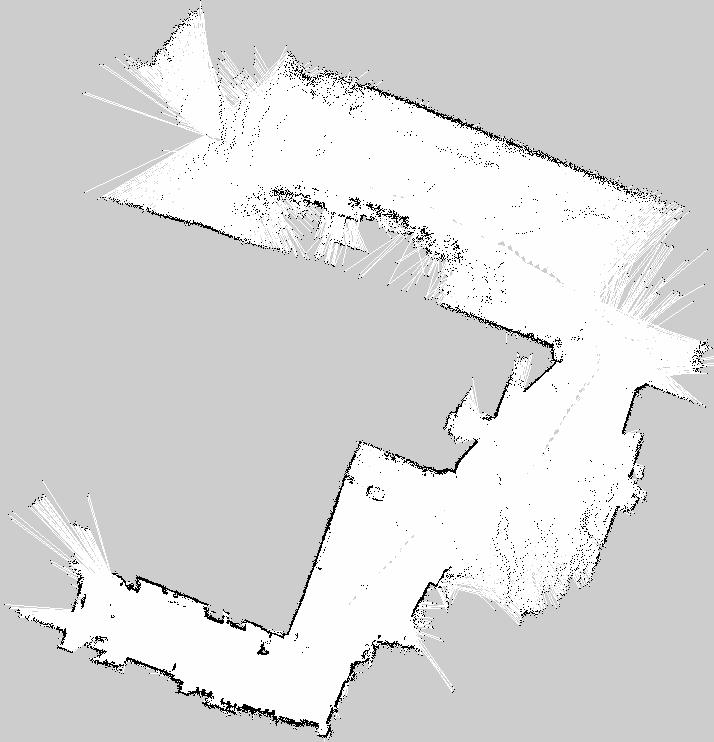
\includegraphics[width=1\textwidth]{Meresek/SLAM/terkep1.jpg}};
    \begin{scope}[x={(image.south east)},y={(image.north west)}]
         \draw[fill=green,ultra thick,rounded corners] (0.42,0.06) rectangle (0.38,0.09);
         \draw[fill=red,ultra thick,rounded corners] (0.27,0.83) rectangle (0.23,0.86);
         %\draw[help lines,xstep=.1,ystep=.1] (0,0) grid (1,1);

		 \node[draw,align=left] at (0.5,0.6) {Fuves Rész}

		  \begin{axis}[
		  	,width=17cm
       		,height=17cm
       	   ,ylabel={\bfseries{\emph{[m]}}}
           ,xlabel={\bfseries{\emph{[m]}}}
           ,ylabel style={rotate=-90}
           ,grid=both
           ,every both grid/.style={gray, opacity=0.9}
    	   ,grid style={line width=.9pt, draw=gray!10}
		  ]
		 \addplot [color=blue,each nth point={10}] table [header=true, x=poseX, y=poseY]
		  {\pos};
		  \end{axis}
    \end{scope}
   
    
\end{tikzpicture}


   
     
    % Caption
    \ifthenelse{\equal{\captionn}{*}}
    {}
    {\captionof{figure}{\captionn}}
    \renewcommand{\captionn}{*}
    \label{fig:\figlabel}
    

\end{figure}



\iffalse

\renewcommand{\GlobalPath}{Meresek/Mozgasok/NormalMukodes/Korpalya_07_05_Kavicsos}
\renewcommand{\GlobalPathA}{Meresek/Mozgasok/NormalMukodes/Korpalya_07_03_Kavicsos}
\renewcommand{\palya}{50/15}
\renewcommand{\palyaA}{50/25}
\renewcommand{\figlabel}{KorpalyakKavicsos}
\renewcommand{\nth}{5}
\renewcommand{\coefA}{-1}
\renewcommand{\coefB}{1}
\renewcommand{\coefC}{1}
        %-------------------------------------------------Palya Adatok---------------
        
        \begin{figure}[H]
            \input{\mand{\GlobalPath}{/Pos.tex}}
            \pgfplotstableread{PositionOrientation.dat}{\position}
            
            \ifthenelse{\equal{\GlobalPathA}{*}}
            {}
            {
                \input{\mand{\GlobalPathA}{/Pos.tex}}
                \pgfplotstableread{PositionOrientation.dat}{\positionA}
            }
            
            \ifthenelse{\equal{\GlobalPathB}{*}}
            {}
            {
                \input{\mand{\GlobalPathB}{/Pos.tex}}
                \pgfplotstableread{PositionOrientation.dat}{\positionB}
            }
            
            \ifthenelse{\equal{\GlobalPathC}{*}}
            {}
            {
                \input{\mand{\GlobalPathC}{/Pos.tex}}
                \pgfplotstableread{PositionOrientation.dat}{\positionC}
            }
            
            \tikzsetnextfilename{\figlabel}
            
            \begin{tikzpicture}
                 \pgfplotsset{every axis plot/.append style={very thick}}
        \pgfplotsset{every axis legend/.append style={
        at={(0.5,1.03)},
        anchor=south}}
        
        \begin{axis}[
                ,width=14.5cm
                ,height=15cm
                ,try min ticks=5
                ,xlabel={\bfseries{\emph{\idoFelirat}}}
                %,ylabel={\bfseries{\emph{A}}}
                %,zlabel={\bfseries{\emph{kg}}}
                ,grid=both
                ,every both grid/.style={gray, opacity=0.5}
                ,view={0}{90},
                %,xtick distance=10
                %,ytick distance=20
                %,minor tick num=5
                %xmin=0,xmax=0.65,
                %ymin=0,ymax=0.65,
                %zmin=-5,zmax=60,
                ,legend columns=-1
              ]
              
            	\addplot [color=red,each nth point={\nth}] table [header=true, x=poseX, y=poseY] {\position};
            	
				\ifthenelse{\equal{\GlobalPathA}{*}}
    			{}
    			{
            		\addplot [color=blue,each nth point={\nth}] table [header=true, x=poseX, y expr=\thisrow{poseY}*\coefA] {\positionA};
            	}
            	
            	\ifthenelse{\equal{\GlobalPathB}{*}}
    			{}
    			{
            		\addplot [color=green,each nth point={\nth}] table [header=true, x=poseX, y=poseY] {\positionB};
            	}
            	
            	
            	\ifthenelse{\equal{\GlobalPathC}{*}}
    			{}
    			{
            		\addplot [color=black,each nth point={\nth}] table [header=true, x=poseX, y=poseY] {\positionC};
            	}            	
            
            	
            	\legend
            	{
            	    \bfseries{\emph{\palya}},
					\ifthenelse{\equal{\GlobalPathA}{*}}
    				{}
    				{
            			\bfseries{\emph{\palyaA}}
            		}            		
            		\ifthenelse{\equal{\GlobalPathB}{*}}
    				{}
    				{
            			\bfseries{\emph{\palyaB}}
            		}          		           		
            		\ifthenelse{\equal{\GlobalPathC}{*}}
    				{}
    				{
            			\bfseries{\emph{\palyaC}}
            		}             		         	
            	}
         
         \end{axis}
            \end{tikzpicture}
    \end{figure}
    
    \renewcommand{\palya}{*}
    \renewcommand{\palyaA}{*}
    \renewcommand{\palyaB}{*}
    \renewcommand{\palyaC}{*}
    
    \renewcommand{\GlobalPath}{*}
    \renewcommand{\GlobalPathA}{*}
    \renewcommand{\GlobalPathB}{*}
    \renewcommand{\GlobalPathC}{*}
    
    \renewcommand{\figlabel}{*}
    \renewcommand{\figlabela}{*}
    \renewcommand{\figlabelb}{*}
    \renewcommand{\figlabelc}{*}
    
        



\renewcommand{\GlobalPath}{Meresek/Mozgasok/Lepcso/Le/}

\renewcommand{\figlabel}{LepcsoLexx}
\renewcommand{\nth}{2}
\begin{figure}[H]
    %\ContinuedFloat
    %-------------------------------------------------Pozicio X es Y Adatok---------------
   % \newline

	\input{ \mand{\GlobalPath}{L.tex} }
	\pgfplotstableread{NodeLeft.dat}{\leftNode}


	\input{\mand{\GlobalPath}{R.tex}}
	\pgfplotstableread{NodeRight.dat}{\rightNode}

    
    \tikzsetnextfilename{\figlabel}
    
    \begin{tikzpicture}
    
            \pgfplotsset{every axis plot/.append style={very thick}}
            \setcaptionsubtype
       \begin{groupplot}[%
                        ,group style={%
                            ,group name=my plots
                            ,group size=2 by 2
                            ,vertical sep=1.8cm,
                            ,horizontal sep = 2.4cm,
                            ,ylabels at=edge left
                        }
                        ,width=7cm
                        ,height=6cm
                        ,try min ticks=5
                        ,xlabel={\bfseries{\emph{\idoFelirat}}}
                        ,zlabel={\bfseries{\emph{kg}}}
                        %%ha kell y felirat az elso ketore
                        %,ylabel={\bfseries{\degree$/s$}}
                        %,ylabel style={rotate=-90}
                        %,xtick={0,10,...,60},
                        %,minor tick num=5
                        %,xtick distance=10
                        %,ytick distance=25
                        ,grid=major%both
                        ,every both grid/.style={gray, opacity=0.7},
                        view={0}{90},
                        legend columns=2,
                        %xmin=0,xmax=0.65,
                        %ymin=0,ymax=0.65,
                       % zmin=-5,zmax=60,
                        ]
            %% ide jonnek a adatok. 
            
            %ha kell felirat be kell teni a nextplot[] parameterei koze
            % \nextgroupplot[ylabel=\degree$/s$, ylabel style={rotate=-90},legend to name={CommonLegend},legend style={legend columns=2}]
            \nextgroupplot[]
                \addplot [color=black,each nth point={\nth}] table [header=true, x=Time, y=effortA] {\leftNode};\label{plots:plot4}
                \addplot [color=blue,each nth point={\nth}] table [header=true, x=Time, y=omegaA] {\leftNode}; \label{plots:plot1}
                \addplot [color=red,each nth point={\nth}] table [header=true, x=Time, y=pwmA] {\leftNode};\label{plots:plot2}
                \addplot [color=green,each nth point={\nth}] table [header=true, x=Time, y=refOmegaA] {\leftNode};\label{plots:plot3}
                \coordinate (top) at (rel axis cs:0,1);% coordinate at top of the first plot
            
            \nextgroupplot[]
                \addplot [color=black,each nth point={\nth}] table [header=true, x=Time, y=effortA] {\rightNode};
                \addplot [color=blue,each nth point={\nth}] table [header=true, x=Time, y=omegaA] {\rightNode};
                \addplot [color=red,each nth point={\nth}] table [header=true, x=Time, y=pwmA] {\rightNode};
                \addplot [color=green,each nth point={\nth}] table [header=true, x=Time, y=refOmegaA] {\rightNode};
                    
            \nextgroupplot[]
                \addplot [color=black,each nth point={\nth}] table [header=true, x=Time, y=effortB] {\leftNode};
                \addplot [color=blue,each nth point={\nth}] table [header=true, x=Time, y=omegaB] {\leftNode};
                \addplot [color=red,each nth point={\nth}] table [header=true, x=Time, y=pwmB] {\leftNode};
                \addplot [color=green,each nth point={\nth}] table [header=true, x=Time, y=refOmegaB] {\leftNode};
                   
            \nextgroupplot[]
                \addplot [color=black,each nth point={\nth}] table [header=true, x=Time, y=effortB] {\rightNode};
                \addplot [color=blue,each nth point={\nth}] table [header=true, x=Time, y=omegaB] {\rightNode};
                \addplot [color=red,each nth point={\nth}] table [header=true, x=Time, y=pwmB] {\rightNode};
                \addplot [color=green,each nth point={\nth}] table [header=true, x=Time, y=refOmegaB] {\rightNode};
                \coordinate (bot) at (rel axis cs:1,0);% coordinate at bottom of the last plot
            \end{groupplot}
            
            %\path [nodes={anchor=south,rotate=90,font=\large\bfseries,midway}]
            %  (my plots c1r1.outer north west)--(my plots c1r2.outer south west)
            %    node {Testing of Parameters 1}
            %  (my plots c2r1.outer north west)--(my plots c2r2.outer south west)
            %    node {Testing of Parameters 2};
            
            % legend
            \node[text width=.5\linewidth,align=center,anchor=south] at (my plots c1r1.north) {\caption[]{FL\label{subplot:one}}};
            \node[text width=.5\linewidth,align=center,anchor=south] at (my plots c2r1.north) {\caption[]{FR\label{subplot:two}}};
            \node[text width=.5\linewidth,align=center,anchor=south] at (my plots c1r2.north) {\caption[]{BL\label{subplot:three}}};
            \node[text width=.5\linewidth,align=center,anchor=south] at (my plots c2r2.north) {\caption[]{BR\label{subplot:four}}};
            
            %\path (top-|current bounding box.west)-- 
            %      node[anchor=south,rotate=90] {throughput} 
            %      (bot-|current bounding box.west);
            % legend
            \path (top|-current bounding box.north)--
                  coordinate(legendpos)
                  (bot|-current bounding box.north);
            \matrix[
                matrix of nodes,
                anchor=south,
                draw,
                inner sep=0.2em,
                draw
              ]at([yshift=1ex]legendpos)
              {
                \ref{plots:plot1}& Aktualis Szogsebesseg [\degree/s]&[5pt]
                \ref{plots:plot2}& PWM [\%] &[5pt]
                \ref{plots:plot3}& Eloirt Omega [\degree/s] &[5pt]
                \ref{plots:plot4}& Energia [Watt] &[5pt]\\
            };
    \end{tikzpicture}

    
    % Caption
    %\ifthenelse{\equal{\captionn}{*}}
    %{}
    %{\captionof{figure}{\captionn}}
    %\renewcommand{\captionn}{*}
    %\label{subplot:\figlabel}
    
\end{figure}

    


\renewcommand{\figlabel}{ImuLepcsoLe1}
\renewcommand{\nth}{2}
   
    
    \begin{figure}[H]
        %\ContinuedFloat
        
            \tikzsetnextfilename{\figlabel}   
    
            \centering
             \input{\mand{\GlobalPath}{ImuA.tex}}
            \pgfplotstableread{ImuA.dat}{\imua}
            
            
             \begin{tikzpicture}
    
        \pgfplotsset{every axis plot/.append style={very thick}}
        \pgfplotsset{every axis legend/.append style={
        at={(0.5,1.03)},
        anchor=south}}
        
        \begin{axis}[
                ,width=14.5cm
                ,height=10cm
                ,try min ticks=5
                ,xlabel={\bfseries{\emph{\idoFelirat}}}
                ,ylabel={\bfseries{\emph{$m/{s^2}$}}}
                %,zlabel={\bfseries{\emph{kg}}}
                ,grid=both
                ,every both grid/.style={gray, opacity=0.5}
                ,view={0}{90},
                %,xtick distance=10
                %,ytick distance=20
                %,minor tick num=5
                %xmin=0,xmax=0.65,
                %ymin=0,ymax=0.65,
                %zmin=-5,zmax=60,
                ,legend columns=-1
              ]
              
               \addplot [color=red,each nth point={\nth}] table [header=true, x=Time, y expr=\thisrow{aX}] {\imua}; \addlegendentry {aX}
                            \addplot [color=blue,each nth point={\nth}] table [header=true, x=Time, y expr=\thisrow{aY}] {\imua}; \addlegendentry {aY}
                            \addplot [color=green,each nth point={\nth}] table [header=true, x=Time, y expr=\thisrow{aZ}] {\imua}; \addlegendentry {aZ}
            %\legend{\bfseries{\emph{Pozíció X}},\bfseries{\emph{Pozíció Y}}}
         
         \end{axis}
    \end{tikzpicture}
    
    \end{figure}


\renewcommand{\GlobalPath}{Meresek/Mozgasok/Lepcso/Fel/}

\renewcommand{\figlabel}{LepcsoFelxx}
\renewcommand{\nth}{2}
\begin{figure}[H]
    %\ContinuedFloat
    %-------------------------------------------------Pozicio X es Y Adatok---------------
   % \newline

	\input{ \mand{\GlobalPath}{L.tex} }
	\pgfplotstableread{NodeLeft.dat}{\leftNode}


	\input{\mand{\GlobalPath}{R.tex}}
	\pgfplotstableread{NodeRight.dat}{\rightNode}

    
    \tikzsetnextfilename{\figlabel}
    
    \begin{tikzpicture}
    
            \pgfplotsset{every axis plot/.append style={very thick}}
            \setcaptionsubtype
       \begin{groupplot}[%
                        ,group style={%
                            ,group name=my plots
                            ,group size=2 by 2
                            ,vertical sep=1.8cm,
                            ,horizontal sep = 2.4cm,
                            ,ylabels at=edge left
                        }
                        ,width=7cm
                        ,height=6cm
                        ,try min ticks=5
                        ,xlabel={\bfseries{\emph{\idoFelirat}}}
                        ,zlabel={\bfseries{\emph{kg}}}
                        %%ha kell y felirat az elso ketore
                        %,ylabel={\bfseries{\degree$/s$}}
                        %,ylabel style={rotate=-90}
                        %,xtick={0,10,...,60},
                        %,minor tick num=5
                        %,xtick distance=10
                        %,ytick distance=25
                        ,grid=major%both
                        ,every both grid/.style={gray, opacity=0.7},
                        view={0}{90},
                        legend columns=2,
                        %xmin=0,xmax=0.65,
                        %ymin=0,ymax=0.65,
                       % zmin=-5,zmax=60,
                        ]
            %% ide jonnek a adatok. 
            
            %ha kell felirat be kell teni a nextplot[] parameterei koze
            % \nextgroupplot[ylabel=\degree$/s$, ylabel style={rotate=-90},legend to name={CommonLegend},legend style={legend columns=2}]
            \nextgroupplot[]
                \addplot [color=black,each nth point={\nth}] table [header=true, x=Time, y=effortA] {\leftNode};\label{plots:plot4}
                \addplot [color=blue,each nth point={\nth}] table [header=true, x=Time, y=omegaA] {\leftNode}; \label{plots:plot1}
                \addplot [color=red,each nth point={\nth}] table [header=true, x=Time, y=pwmA] {\leftNode};\label{plots:plot2}
                \addplot [color=green,each nth point={\nth}] table [header=true, x=Time, y=refOmegaA] {\leftNode};\label{plots:plot3}
                \coordinate (top) at (rel axis cs:0,1);% coordinate at top of the first plot
            
            \nextgroupplot[]
                \addplot [color=black,each nth point={\nth}] table [header=true, x=Time, y=effortA] {\rightNode};
                \addplot [color=blue,each nth point={\nth}] table [header=true, x=Time, y=omegaA] {\rightNode};
                \addplot [color=red,each nth point={\nth}] table [header=true, x=Time, y=pwmA] {\rightNode};
                \addplot [color=green,each nth point={\nth}] table [header=true, x=Time, y=refOmegaA] {\rightNode};
                    
            \nextgroupplot[]
                \addplot [color=black,each nth point={\nth}] table [header=true, x=Time, y=effortB] {\leftNode};
                \addplot [color=blue,each nth point={\nth}] table [header=true, x=Time, y=omegaB] {\leftNode};
                \addplot [color=red,each nth point={\nth}] table [header=true, x=Time, y=pwmB] {\leftNode};
                \addplot [color=green,each nth point={\nth}] table [header=true, x=Time, y=refOmegaB] {\leftNode};
                   
            \nextgroupplot[]
                \addplot [color=black,each nth point={\nth}] table [header=true, x=Time, y=effortB] {\rightNode};
                \addplot [color=blue,each nth point={\nth}] table [header=true, x=Time, y=omegaB] {\rightNode};
                \addplot [color=red,each nth point={\nth}] table [header=true, x=Time, y=pwmB] {\rightNode};
                \addplot [color=green,each nth point={\nth}] table [header=true, x=Time, y=refOmegaB] {\rightNode};
                \coordinate (bot) at (rel axis cs:1,0);% coordinate at bottom of the last plot
            \end{groupplot}
            
            %\path [nodes={anchor=south,rotate=90,font=\large\bfseries,midway}]
            %  (my plots c1r1.outer north west)--(my plots c1r2.outer south west)
            %    node {Testing of Parameters 1}
            %  (my plots c2r1.outer north west)--(my plots c2r2.outer south west)
            %    node {Testing of Parameters 2};
            
            % legend
            \node[text width=.5\linewidth,align=center,anchor=south] at (my plots c1r1.north) {\caption[]{FL\label{subplot:one}}};
            \node[text width=.5\linewidth,align=center,anchor=south] at (my plots c2r1.north) {\caption[]{FR\label{subplot:two}}};
            \node[text width=.5\linewidth,align=center,anchor=south] at (my plots c1r2.north) {\caption[]{BL\label{subplot:three}}};
            \node[text width=.5\linewidth,align=center,anchor=south] at (my plots c2r2.north) {\caption[]{BR\label{subplot:four}}};
            
            %\path (top-|current bounding box.west)-- 
            %      node[anchor=south,rotate=90] {throughput} 
            %      (bot-|current bounding box.west);
            % legend
            \path (top|-current bounding box.north)--
                  coordinate(legendpos)
                  (bot|-current bounding box.north);
            \matrix[
                matrix of nodes,
                anchor=south,
                draw,
                inner sep=0.2em,
                draw
              ]at([yshift=1ex]legendpos)
              {
                \ref{plots:plot1}& Aktualis Szogsebesseg [\degree/s]&[5pt]
                \ref{plots:plot2}& PWM [\%] &[5pt]
                \ref{plots:plot3}& Eloirt Omega [\degree/s] &[5pt]
                \ref{plots:plot4}& Energia [Watt] &[5pt]\\
            };
    \end{tikzpicture}

    
    % Caption
    %\ifthenelse{\equal{\captionn}{*}}
    %{}
    %{\captionof{figure}{\captionn}}
    %\renewcommand{\captionn}{*}
    %\label{subplot:\figlabel}
    
\end{figure}

    


\renewcommand{\figlabel}{ImuLepcsoFel1}
\renewcommand{\nth}{2}
   
    
    \begin{figure}[H]
        %\ContinuedFloat
        
            \tikzsetnextfilename{\figlabel}   
    
            \centering
             \input{\mand{\GlobalPath}{ImuA.tex}}
            \pgfplotstableread{ImuA.dat}{\imua}
            
            
             \begin{tikzpicture}
    
        \pgfplotsset{every axis plot/.append style={very thick}}
        \pgfplotsset{every axis legend/.append style={
        at={(0.5,1.03)},
        anchor=south}}
        
        \begin{axis}[
                ,width=14.5cm
                ,height=10cm
                ,try min ticks=5
                ,xlabel={\bfseries{\emph{\idoFelirat}}}
                ,ylabel={\bfseries{\emph{$m/{s^2}$}}}
                %,zlabel={\bfseries{\emph{kg}}}
                ,grid=both
                ,every both grid/.style={gray, opacity=0.5}
                ,view={0}{90},
                %,xtick distance=10
                %,ytick distance=20
                %,minor tick num=5
                %xmin=0,xmax=0.65,
                %ymin=0,ymax=0.65,
                %zmin=-5,zmax=60,
                ,legend columns=-1
              ]
              
               \addplot [color=red,each nth point={\nth}] table [header=true, x=Time, y expr=\thisrow{aX}] {\imua}; \addlegendentry {aX}
                            \addplot [color=blue,each nth point={\nth}] table [header=true, x=Time, y expr=\thisrow{aY}] {\imua}; \addlegendentry {aY}
                            \addplot [color=green,each nth point={\nth}] table [header=true, x=Time, y expr=\thisrow{aZ}] {\imua}; \addlegendentry {aZ}
            %\legend{\bfseries{\emph{Pozíció X}},\bfseries{\emph{Pozíció Y}}}
         
         \end{axis}
    \end{tikzpicture}
    
    \end{figure}



\renewcommand{\GlobalPath}{Meresek/Mozgasok/HomokosDomb/}
\renewcommand{\figlabel}{HlejtoKerek}
\renewcommand{\nth}{2}
%\begin{figure}[H]
    %\ContinuedFloat
    %-------------------------------------------------Pozicio X es Y Adatok---------------
   % \newline

	\input{ \mand{\GlobalPath}{L.tex} }
	\pgfplotstableread{NodeLeft.dat}{\leftNode}


	\input{\mand{\GlobalPath}{R.tex}}
	\pgfplotstableread{NodeRight.dat}{\rightNode}

    
    \tikzsetnextfilename{\figlabel}
    
    \begin{tikzpicture}
    
            \pgfplotsset{every axis plot/.append style={very thick}}
            \setcaptionsubtype
       \begin{groupplot}[%
                        ,group style={%
                            ,group name=my plots
                            ,group size=2 by 2
                            ,vertical sep=1.8cm,
                            ,horizontal sep = 2.4cm,
                            ,ylabels at=edge left
                        }
                        ,width=7cm
                        ,height=6cm
                        ,try min ticks=5
                        ,xlabel={\bfseries{\emph{\idoFelirat}}}
                        ,zlabel={\bfseries{\emph{kg}}}
                        %%ha kell y felirat az elso ketore
                        %,ylabel={\bfseries{\degree$/s$}}
                        %,ylabel style={rotate=-90}
                        %,xtick={0,10,...,60},
                        %,minor tick num=5
                        %,xtick distance=10
                        %,ytick distance=25
                        ,grid=major%both
                        ,every both grid/.style={gray, opacity=0.7},
                        view={0}{90},
                        legend columns=2,
                        %xmin=0,xmax=0.65,
                        %ymin=0,ymax=0.65,
                       % zmin=-5,zmax=60,
                        ]
            %% ide jonnek a adatok. 
            
            %ha kell felirat be kell teni a nextplot[] parameterei koze
            % \nextgroupplot[ylabel=\degree$/s$, ylabel style={rotate=-90},legend to name={CommonLegend},legend style={legend columns=2}]
            \nextgroupplot[]
                \addplot [color=black,each nth point={\nth}] table [header=true, x=Time, y=effortA] {\leftNode};\label{plots:plot4}
                \addplot [color=blue,each nth point={\nth}] table [header=true, x=Time, y=omegaA] {\leftNode}; \label{plots:plot1}
                \addplot [color=red,each nth point={\nth}] table [header=true, x=Time, y=pwmA] {\leftNode};\label{plots:plot2}
                \addplot [color=green,each nth point={\nth}] table [header=true, x=Time, y=refOmegaA] {\leftNode};\label{plots:plot3}
                \coordinate (top) at (rel axis cs:0,1);% coordinate at top of the first plot
            
            \nextgroupplot[]
                \addplot [color=black,each nth point={\nth}] table [header=true, x=Time, y=effortA] {\rightNode};
                \addplot [color=blue,each nth point={\nth}] table [header=true, x=Time, y=omegaA] {\rightNode};
                \addplot [color=red,each nth point={\nth}] table [header=true, x=Time, y=pwmA] {\rightNode};
                \addplot [color=green,each nth point={\nth}] table [header=true, x=Time, y=refOmegaA] {\rightNode};
                    
            \nextgroupplot[]
                \addplot [color=black,each nth point={\nth}] table [header=true, x=Time, y=effortB] {\leftNode};
                \addplot [color=blue,each nth point={\nth}] table [header=true, x=Time, y=omegaB] {\leftNode};
                \addplot [color=red,each nth point={\nth}] table [header=true, x=Time, y=pwmB] {\leftNode};
                \addplot [color=green,each nth point={\nth}] table [header=true, x=Time, y=refOmegaB] {\leftNode};
                   
            \nextgroupplot[]
                \addplot [color=black,each nth point={\nth}] table [header=true, x=Time, y=effortB] {\rightNode};
                \addplot [color=blue,each nth point={\nth}] table [header=true, x=Time, y=omegaB] {\rightNode};
                \addplot [color=red,each nth point={\nth}] table [header=true, x=Time, y=pwmB] {\rightNode};
                \addplot [color=green,each nth point={\nth}] table [header=true, x=Time, y=refOmegaB] {\rightNode};
                \coordinate (bot) at (rel axis cs:1,0);% coordinate at bottom of the last plot
            \end{groupplot}
            
            %\path [nodes={anchor=south,rotate=90,font=\large\bfseries,midway}]
            %  (my plots c1r1.outer north west)--(my plots c1r2.outer south west)
            %    node {Testing of Parameters 1}
            %  (my plots c2r1.outer north west)--(my plots c2r2.outer south west)
            %    node {Testing of Parameters 2};
            
            % legend
            \node[text width=.5\linewidth,align=center,anchor=south] at (my plots c1r1.north) {\caption[]{FL\label{subplot:one}}};
            \node[text width=.5\linewidth,align=center,anchor=south] at (my plots c2r1.north) {\caption[]{FR\label{subplot:two}}};
            \node[text width=.5\linewidth,align=center,anchor=south] at (my plots c1r2.north) {\caption[]{BL\label{subplot:three}}};
            \node[text width=.5\linewidth,align=center,anchor=south] at (my plots c2r2.north) {\caption[]{BR\label{subplot:four}}};
            
            %\path (top-|current bounding box.west)-- 
            %      node[anchor=south,rotate=90] {throughput} 
            %      (bot-|current bounding box.west);
            % legend
            \path (top|-current bounding box.north)--
                  coordinate(legendpos)
                  (bot|-current bounding box.north);
            \matrix[
                matrix of nodes,
                anchor=south,
                draw,
                inner sep=0.2em,
                draw
              ]at([yshift=1ex]legendpos)
              {
                \ref{plots:plot1}& Aktualis Szogsebesseg [\degree/s]&[5pt]
                \ref{plots:plot2}& PWM [\%] &[5pt]
                \ref{plots:plot3}& Eloirt Omega [\degree/s] &[5pt]
                \ref{plots:plot4}& Energia [Watt] &[5pt]\\
            };
    \end{tikzpicture}

    
    % Caption
    %\ifthenelse{\equal{\captionn}{*}}
    %{}
    %{\captionof{figure}{\captionn}}
    %\renewcommand{\captionn}{*}
    %\label{subplot:\figlabel}
    
\end{figure}

    



\begin{figure}[H]
  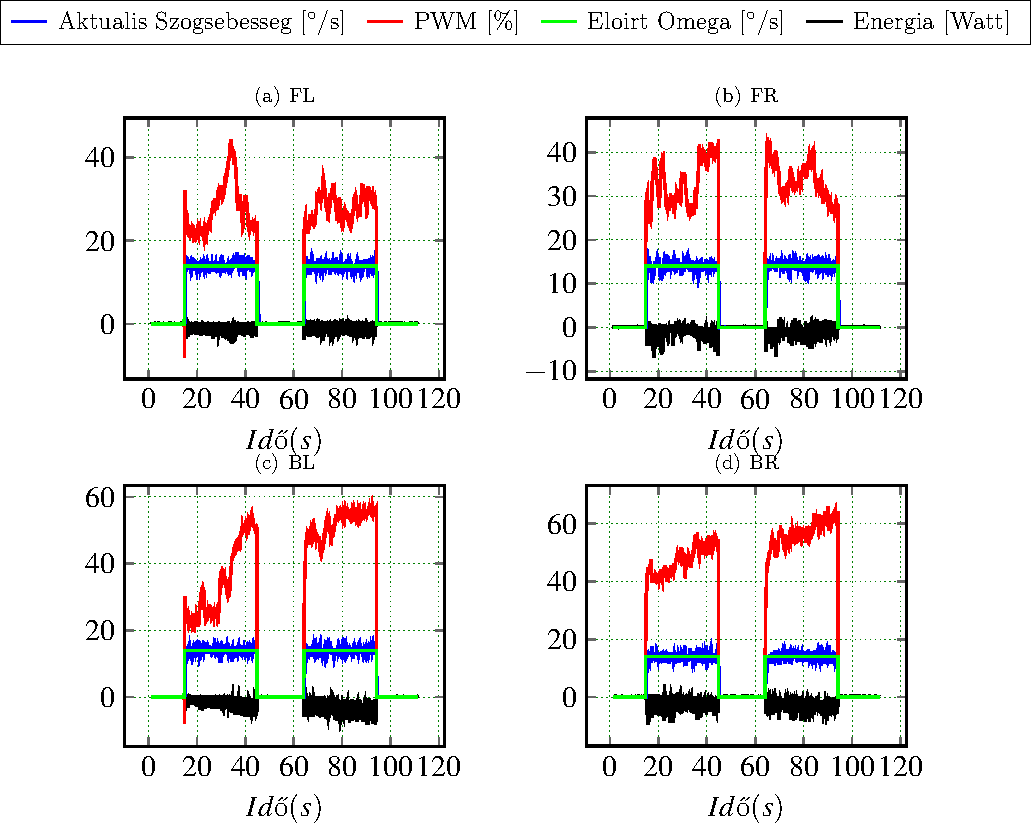
\includegraphics{tikz/HlejtoKerek.pdf}
  \caption{}
  \label{fig:HlejtoKerek}
\end{figure}


\renewcommand{\nth}{10}
\begin{filecontents}{TfSysIdent.dat}
Time PWM Omega sysResp
   0.58281    0.00000    0.00000    5.87602
   0.63400   20.00000    0.00000    5.53891
   0.69486   20.00000    4.79996    6.21402
   0.74558   20.00000   12.52029    9.50791
   0.79625   20.00000   17.21962   13.53107
   0.84705   20.00000   21.21399   16.86729
   0.88778   20.00000   23.59718   19.26695
   0.93843   20.00000   25.07416   21.01915
   0.98942   20.00000   26.55098   22.40958
   1.03015   20.00000   26.98746   23.57178
   1.10136   20.00000   27.72583   24.54385
   1.14217   20.00000   28.59863   25.34152
   1.19277   20.00000   29.63913   25.98714
   1.24345   20.00000   28.16223   26.50836
   1.29428   20.00000   31.18324   26.93067
   1.33494   20.00000   28.73283   27.27408
   1.38584   20.00000   31.82098   27.55364
   1.43684   20.00000   31.41823   27.78110
   1.49799   20.00000   29.50485   27.96599
   1.54909   20.00000   32.42523   28.11623
   1.58974   20.00000   29.97482   28.23832
   1.64042   20.00000   32.52586   28.33754
   1.69123   20.00000   32.62657   28.41821
   1.74212   20.00000   29.50485   28.48377
   1.78279   20.00000   32.62665   28.53707
   1.83383   20.00000   29.23630   28.58039
   1.89501   20.00000   32.05597   28.61560
   1.94580   20.00000   30.67978   28.64422
   1.99671   20.00000   30.91461   28.66749
   2.03747   20.00000   32.35809   28.68640
   2.08847   20.00000   30.91461   28.70177
   2.13953   20.00000   31.35101   28.71426
   2.19037   20.00000   32.79449   28.72442
   2.23099   20.00000   30.44479   28.73267
   2.30207   20.00000   30.10895   28.73938
   2.34273   20.00000   33.26447   28.74483
   2.39354   20.00000   29.87411   28.74927
   2.44409   20.00000   29.50485   28.75287
   2.49480   20.00000   30.98175   28.75580
   2.53559   20.00000   30.64621   28.75818
   2.58646   20.00000   31.21674   28.76011
   2.63722   20.00000   30.78049   28.76169
   2.69831   20.00000   31.75385   28.76296
   2.74913   20.00000   31.55243   28.76400
   2.78954   20.00000   30.20981   28.76485
   2.84029   20.00000   31.82098   28.76553
   2.89118   20.00000   30.27695   28.76609
   2.94209   20.00000   30.88104   28.76655
   2.98305   20.00000   29.53842   28.76691
   3.03401   20.00000   28.19580   28.76721
   3.09490   20.00000   31.51901   28.76746
   3.14588   20.00000   30.44464   28.76766
   3.19674   20.00000   28.09509   28.76782
   3.23752   20.00000   30.07553   28.76795
   3.28833   20.00000   31.01547   28.76805
   3.33928   20.00000   29.10202   28.76814
   3.39020   20.00000   31.92169   28.76821
   3.43106   20.00000   29.20288   28.76827
   3.50227   20.00000   30.24323   28.76831
   3.54292   20.00000   29.43787   28.76835
   3.59354   20.00000   28.22937   28.76838
   3.64426   20.00000   32.08954   28.76841
   3.68507   20.00000   27.22229   28.76843
   3.73615   20.00000   29.16931   28.76844
   3.78698   20.00000   29.03488   28.76846
   3.83776   20.00000   28.90076   28.76847
   3.89930   20.00000   29.30344   28.76848
   3.95021   20.00000   30.91461   28.76848
   3.99075   20.00000   28.93433   28.76849
   4.04142   20.00000   31.41815   28.76850
   4.09250   20.00000   27.75940   28.76850
   4.13318   20.00000   29.16931   28.76850
   4.18432   20.00000   29.33716   28.76850
   4.23501   20.00000   27.89368   28.76851
   4.29619   20.00000   29.16931   28.76851
   4.34680   20.00000   27.86011   28.76851
   4.39771   20.00000   29.20258   28.76851
   4.43840   20.00000   28.29651   28.76851
   4.48917   20.00000   29.80713   28.76851
   4.53993   20.00000   28.59863   28.76851
   4.59069   20.00000   29.40399   28.76851
   4.65216   20.00000   29.00146   28.76851
   4.70297   20.00000   30.20996   28.76851
   4.74407   20.00000   27.96082   28.76851
   4.79469   20.00000   29.57184   28.76851
   4.84524   20.00000   26.45050   28.76852
   4.88606   20.00000   30.84747   28.76852
   4.93673   20.00000   27.15515   28.76852
   4.98748   20.00000   29.43787   28.76852
   5.04858   20.00000   27.45728   28.76852
   5.09964   20.00000   27.18903   28.76852
   5.15044   20.00000   29.40399   28.76852
   5.19090   20.00000   32.39166   28.76852
   5.24174   20.00000   24.33563   28.76852
   5.29249   20.00000   30.17639   28.76852
   5.33309   20.00000   30.67963   28.76852
   5.38385   20.00000   27.92725   28.76852
   5.43456   20.00000   29.23645   28.76852
   5.49570   20.00000   28.16223   28.76852
   5.54646   20.00000   29.40399   28.76852
   5.59755   20.00000   28.16223   28.76852
   5.63832   20.00000   28.59863   28.76852
   5.68937   20.00000   28.39722   28.76852
   5.74021   20.00000   29.06860   28.76852
   5.78102   20.00000   27.99438   28.76852
   5.85222   20.00000   30.07568   28.76852
   5.89300   20.00000   29.53827   28.76852
   5.94390   20.00000   29.57214   28.76852
   5.99435   20.00000   28.09509   28.76852
   6.04506   20.00000   31.65314   28.76852
   6.08576   20.00000   28.02795   28.76852
   6.13669    0.00000   31.28387   28.76852
   6.18772    0.00000   26.61835   27.17744
   6.23849    0.00000   23.26141   22.85431
   6.29959    0.00000   18.02521   17.99650
   6.35063    0.00000   13.93005   14.05713
   6.39127    0.00000    8.99567   11.21038
   6.44182    0.00000    4.29657    9.10023
   6.49270    0.00000    0.63782    7.41077
   6.53346    0.00000    0.00000    5.99939
   6.58436    0.00000    0.03357    4.82335
   6.63508    0.00000    0.00000    3.86064
   6.69601    0.00000    0.00000    3.08168
   6.74700    0.00000    0.03357    2.45236
   6.79790    0.00000    0.00000    1.94212
   6.83848    0.00000    0.00000    1.52715
   6.88940    0.00000    0.00000    1.18936
   6.94022    0.00000    0.00000    0.91459
   6.98119    0.00000    0.00000    0.69124
   7.03200    0.00000    0.00000    0.50976
   7.09292    0.00000    0.00000    0.36227
   7.14386    0.00000    0.00000    0.24240
   7.19469    0.00000    0.00000    0.14495
   7.24534    0.00000    0.00000    0.06574
   7.28623    0.00000    0.00000    0.00136
   7.33712    0.00000    0.00000   -0.05097
   7.38782    0.00000    0.00000   -0.09351
   7.43870    0.00000    0.00000   -0.12809
   7.49995    0.00000    0.00000   -0.15619
   7.54136    0.00000    0.00000   -0.17904
   7.59193    0.00000    0.00000   -0.19760
   7.64253    0.00000    0.00000   -0.21270
   7.69347    0.00000    0.03357   -0.22496
   7.73422    0.00000    0.00000   -0.23493
   7.78522    0.00000    0.00000   -0.24304
   7.83640    0.00000    0.00000   -0.24963
   7.89756    0.00000    0.00000   -0.25498
   7.94848    0.00000    0.00000   -0.25934
   7.98905    0.00000    0.00000   -0.26287
   8.03976    0.00000    0.00000   -0.26575
   8.09088    0.00000    0.00000   -0.26809
   8.14182    0.00000    0.00000   -0.26999
   8.18245    0.00000    0.00000   -0.27153
   8.23320    0.00000    0.00000   -0.27279
   8.29401    0.00000    0.00000   -0.27381
   8.34485    0.00000    0.00000   -0.27464
   8.39584    0.00000    0.00000   -0.27531
   8.44644    0.00000    0.00000   -0.27586
   8.48712    0.00000    0.00000   -0.27630
   8.53809    0.00000    0.00000   -0.27667
   8.58893    0.00000    0.00000   -0.27696
   8.62941    0.00000    0.00000   -0.27720
   8.70068    0.00000    0.00000   -0.27739
   8.74151    0.00000    0.00000   -0.27755
   8.79251    0.00000    0.00000   -0.27768
   8.84295    0.00000    0.00000   -0.27778
   8.89372    0.00000    0.00000   -0.27787
   8.93459    0.00000    0.00000   -0.27794
   8.98558    0.00000    0.00000   -0.27799
   9.03653    0.00000    0.00000   -0.27804
   9.09774    0.00000    0.00000   -0.27808
   9.14869    0.00000    0.00000   -0.27811
   9.18933    0.00000    0.00000   -0.27813
   9.24034    0.00000    0.00000   -0.27815
   9.29110    0.00000    0.00000   -0.27817
   9.34183    0.00000    0.00000   -0.27818
   9.38251    0.00000    0.00000   -0.27819
   9.45382    0.00000    0.00000   -0.27820
   9.49461    0.00000    0.00000   -0.27821
   9.54527    0.00000    0.00000   -0.27821
   9.59595    0.00000    0.00000   -0.27822
   9.64673    0.00000    0.00000   -0.27822
   9.68745    0.00000    0.00000   -0.27822
   9.73825    0.00000    0.00000   -0.27823
   9.78920    0.00000    0.00000   -0.27823
   9.83005    0.00000    0.00000   -0.27823
   9.90134    0.00000    0.00000   -0.27823
   9.94204    0.00000    0.00000   -0.27823
   9.99282    0.00000    0.00000   -0.27823
  10.04355    0.00000    0.00000   -0.27824
  10.09451    0.00000    0.00000   -0.27824
  10.13536    0.00000    0.00000   -0.27824
  10.18618    0.00000    0.00000   -0.27824
  10.23689    0.00000    0.00000   -0.27824
  10.29781    0.00000    0.00000   -0.27824
  10.34851    0.00000    0.00000   -0.27824
  10.38943    0.00000    0.00000   -0.27824
  10.44046    0.00000    0.00000   -0.27824
  10.49104    0.00000    0.00000   -0.27824
  10.54179    0.00000    0.00000   -0.27824
  10.58261    0.00000    0.00000   -0.27824
  10.63347    0.00000    0.00000   -0.27824
  10.69435    0.00000    0.00000   -0.27824
  10.74491    0.00000    0.00000   -0.27824
  10.79562    0.00000    0.00000   -0.27824
  10.84660    0.00000    0.00000   -0.27824
  10.88753    0.00000    0.00000   -0.27824
  10.93866    0.00000    0.00000   -0.27824
  10.98957    0.00000    0.00000   -0.27824
  11.03072    0.00000    0.00000   -0.27824
  11.10227    0.00000    0.00000   -0.27824
  11.14316    0.00000    0.00000   -0.27824
  11.19374    0.00000    0.00000   -0.27824
  11.24453    0.00000    0.00000   -0.27824
  11.28517    0.00000    0.00000   -0.27824
  11.33580    0.00000    0.00000   -0.27824
  11.38666    0.00000    0.00000   -0.27824
  11.44767    0.00000    0.00000   -0.27824
  11.49862    0.00000    0.00000   -0.27824
  11.54945    0.00000    0.00000   -0.27824
  11.59029    0.00000    0.00000   -0.27824
  11.64136    0.00000    0.00000   -0.27824
  11.69217    0.00000    0.00000   -0.27824
  11.73304   30.00000    0.00000   -0.27824
  11.78432   30.00000   10.10345    3.81734
  11.84557   30.00000   25.27557   14.94550
  11.89625   30.00000   30.51178   27.44996
  11.94740   30.00000   37.05750   37.59028
  11.99802   30.00000   36.18469   41.60964
  12.03854   30.00000   40.21240   43.60822
  12.08956   30.00000   43.36792   45.20836
  12.14050   30.00000   42.93152   46.54511
  12.18135   30.00000   44.71039   47.65897
  12.23237   30.00000   43.90503   48.57078
  12.29354   30.00000   47.96631   49.30855
  12.34457   30.00000   46.42242   49.90460
  12.39521   30.00000   48.46985   50.38785
  12.44587   30.00000   48.63770   50.78089
  12.48653   30.00000   48.47015   51.10081
  12.53741   30.00000   53.80676   51.36106
  12.58828   30.00000   46.92596   51.57260
  12.62904   30.00000   49.74548   51.74449
  12.70014   30.00000   49.51050   51.88417
  12.74087   30.00000   51.62506   51.99771
  12.79176   30.00000   50.01404   52.09000
  12.84274   30.00000   52.26288   52.16502
  12.89346   30.00000   51.39038   52.22600
  12.93434   30.00000   53.30353   52.27557
  12.98491   30.00000   52.49786   52.31586
  13.04604   30.00000   52.12830   52.34860
  13.09711   30.00000   53.06885   52.37522
  13.14781   30.00000   51.72607   52.39686
  13.19856   30.00000   53.40393   52.41444
  13.23904   30.00000   54.44458   52.42874
  13.28987   30.00000   52.02820   52.44036
  13.34088   30.00000   52.93396   52.44980
  13.38298   30.00000   53.16956   52.45748
  13.43395   30.00000   52.59827   52.46372
  13.49494   30.00000   54.47876   52.46879
  13.54590   30.00000   54.17603   52.47291
  13.59661   30.00000   54.94812   52.47626
  13.63730   30.00000   52.43103   52.47899
  13.68798   30.00000   55.08240   52.48120
  13.73867   30.00000   51.42395   52.48300
  13.78943   30.00000   55.18311   52.48446
  13.85076   30.00000   54.00818   52.48565
  13.90143   30.00000   54.98169   52.48662
  13.94202   30.00000   54.37805   52.48740
  13.99281   30.00000   56.49231   52.48804
  14.04357   30.00000   52.59827   52.48856
  14.09435   30.00000   54.57947   52.48898
  14.13532   30.00000   54.07532   52.48933
  14.18608   30.00000   55.61951   52.48961
  14.24690   30.00000   52.90100   52.48983
  14.29775   30.00000   57.63306   52.49002
  14.34866   30.00000   53.37097   52.49017
  14.38944   30.00000   52.96753   52.49029
  14.44001   30.00000   54.74731   52.49039
  14.49069   30.00000   55.51880   52.49047
  14.54179   30.00000   53.06824   52.49053
  14.58285   30.00000   54.51172   52.49058
  14.65414   30.00000   54.68018   52.49063
  14.69486   30.00000   54.67957   52.49066
  14.74619   30.00000   54.54529   52.49069
  14.79694   30.00000   53.77380   52.49071
  14.83738   30.00000   53.50464   52.49073
  14.88826   30.00000   55.11597   52.49075
  14.93918   30.00000   54.17603   52.49076
  14.98990   30.00000   54.98230   52.49077
  15.05105   30.00000   51.82657   52.49078
  15.10184   30.00000   54.17622   52.49079
  15.14257   30.00000   52.19580   52.49079
  15.19315   30.00000   55.35106   52.49080
  15.24390   30.00000   54.00839   52.49080
  15.29496   30.00000   54.98182   52.49080
  15.33579   30.00000   56.92867   52.49081
  15.38668   30.00000   52.26292   52.49081
  15.44780   30.00000   51.05453   52.49081
  15.49881   30.00000   52.86713   52.49081
  15.54964   30.00000   55.48534   52.49081
  15.59034   30.00000   52.83356   52.49081
  15.64114   30.00000   53.00140   52.49081
  15.69218   30.00000   55.61958   52.49081
  15.73283   30.00000   50.18181   52.49081
  15.78370   30.00000   52.66571   52.49081
  15.84500   30.00000   52.83356   52.49081
  15.89596   30.00000   52.26295   52.49081
  15.94704   30.00000   52.09511   52.49081
  15.99792   30.00000   54.17625   52.49081
  16.03846   30.00000   49.40979   52.49081
  16.08920   30.00000   53.06847   52.49082
  16.14015   30.00000   48.83919   52.49082
  16.18107   30.00000   52.22939   52.49082
  16.25249   30.00000   50.92026   52.49082
  16.29348   30.00000   51.18881   52.49082
  16.34430   30.00000   50.65170   52.49082
  16.39535   30.00000   52.63214   52.49082
  16.44630   30.00000   49.87976   52.49082
  16.48712   30.00000   51.79306   52.49082
  16.53797   30.00000   49.40979   52.49082
  16.58885   30.00000   49.67834   52.49082
  16.64996   30.00000   51.92719   52.49082
  16.70073   30.00000   50.38330   52.49082
  16.74165   30.00000   50.78598   52.49082
  16.79256   30.00000   49.84619   52.49082
  16.84328   30.00000   50.41672   52.49082
  16.89411   30.00000   48.70483   52.49082
  16.93516    0.00000   50.11475   52.49082
  16.98605    0.00000   44.71054   50.98387
  17.04712    0.00000   44.40826   46.88931
  17.09783    0.00000   36.58752   42.28836
  17.14850    0.00000   31.72028   36.62239
  17.18885    0.00000   27.42371   29.29458
  17.23949    0.00000   20.57632   23.86285
  17.29048    0.00000   16.51459   19.51400
  17.34122    0.00000   11.78192   15.88097
  17.38188    0.00000    7.58591   12.85374
  17.43293    0.00000    2.38327   10.37562
  17.49391    0.00000    0.06714    8.37051
  17.54489    0.00000    0.00000    6.75057
  17.59569    0.00000    0.03357    5.43719
  17.64656    0.00000    0.00000    4.36900
  17.68740    0.00000    0.00000    3.49951
  17.73832    0.00000    0.00000    2.79221
  17.78929    0.00000    0.00000    2.21729
  17.83012    0.00000    0.03357    1.75013
  17.90141    0.00000    0.00000    1.37049
  17.94230    0.00000    0.00000    1.06193
  17.99313    0.00000    0.00000    0.81110
  18.04369    0.00000    0.00000    0.60720
  18.09442    0.00000    0.00000    0.44147
  18.13507    0.00000    0.00000    0.30676
  18.18597    0.00000    0.00000    0.19726
  18.23688    0.00000    0.00000    0.10826
  18.29801    0.00000    0.00000    0.03592
  18.34903    0.00000    0.00000   -0.02288
  18.38975    0.00000    0.00000   -0.07068
  18.44048    0.00000    0.00000   -0.10953
  18.49123    0.00000    0.00000   -0.14110
  18.54180    0.00000    0.00000   -0.16677
  18.58274    0.00000    0.00000   -0.18763
  18.63349    0.00000    0.00000   -0.20459
  18.69449    0.00000    0.00000   -0.21838
  18.74535    0.00000    0.00000   -0.22958
  18.79597    0.00000    0.00000   -0.23869
  18.83665    0.00000    0.00000   -0.24609
  18.88757    0.00000    0.00000   -0.25211
  18.93847    0.00000    0.00000   -0.25700
  18.98943    0.00000    0.00000   -0.26097
  19.03017    0.00000    0.00000   -0.26421
  19.10129    0.00000    0.00000   -0.26683
  19.14241    0.00000    0.00000   -0.26897
  19.19343    0.00000    0.00000   -0.27070
  19.24407    0.00000    0.00000   -0.27211
  19.28483    0.00000    0.00000   -0.27326
  19.33587    0.00000    0.00000   -0.27419
  19.38666    0.00000    0.00000   -0.27495
  19.43756    0.00000    0.00000   -0.27556
  19.49860    0.00000    0.00000   -0.27606
  19.54975    0.00000    0.00000   -0.27647
  19.59076    0.00000    0.00000   -0.27680
  19.64149    0.00000    0.00000   -0.27707
  19.69233    0.00000    0.00000   -0.27729
  19.73327    0.00000    0.00000   -0.27747
  19.78436    0.00000    0.00000   -0.27761
  19.83507    0.00000    0.00000   -0.27773
  19.89626    0.00000    0.00000   -0.27782
  19.94708    0.00000    0.00000   -0.27790
  19.99785    0.00000    0.00000   -0.27796
  20.03876    0.00000    0.00000   -0.27802
  20.08982    0.00000    0.00000   -0.27806
  20.14072    0.00000    0.00000   -0.27809
  20.18143    0.00000    0.00000   -0.27812
  20.23227    0.00000    0.00000   -0.27814
  20.29319    0.00000    0.00000   -0.27816
  20.34464    0.00000    0.00000   -0.27817
  20.39578    0.00000    0.00000   -0.27819
  20.44635    0.00000    0.00000   -0.27820
  20.48702    0.00000    0.00000   -0.27820
  20.53773    0.00000    0.00000   -0.27821
  20.58857    0.00000    0.03357   -0.27822
  20.62931    0.00000    0.00000   -0.27822
  20.70020    0.00000    0.00000   -0.27822
  20.74084    0.00000    0.00000   -0.27823
  20.79165    0.00000    0.00000   -0.27823
  20.84240    0.00000    0.00000   -0.27823
  20.89296    0.00000    0.00000   -0.27823
  20.93364    0.00000    0.00000   -0.27823
  20.98467    0.00000    0.00000   -0.27823
  21.03556    0.00000    0.00000   -0.27823
  21.09665    0.00000    0.00000   -0.27824
  21.14734    0.00000    0.00000   -0.27824
  21.19835    0.00000    0.00000   -0.27824
  21.23914    0.00000    0.00000   -0.27824
  21.28991    0.00000    0.00000   -0.27824
  21.34073    0.00000    0.00000   -0.27824
  21.38153    0.00000    0.00000   -0.27824
  21.43260    0.00000    0.00000   -0.27824
  21.49386    0.00000    0.00000   -0.27824
  21.54486    0.00000    0.00000   -0.27824
  21.59574    0.00000    0.00000   -0.27824
  21.64625    0.00000    0.00000   -0.27824
  21.68680    0.00000    0.00000   -0.27824
  21.73760    0.00000    0.00000   -0.27824
  21.78859    0.00000    0.00000   -0.27824
  21.82940    0.00000    0.00000   -0.27824
  21.90052    0.00000    0.00000   -0.27824
  21.94111    0.00000    0.00000   -0.27824
  21.99170    0.00000    0.00000   -0.27824
  22.04234    0.00000    0.00000   -0.27824
  22.09326    0.00000    0.00000   -0.27824
  22.13401    0.00000    0.00000   -0.27824
  22.18493    0.00000    0.00000   -0.27824
  22.24629    0.00000    0.00000   -0.27824
  22.29732    0.00000    0.00000   -0.27824
  22.34807    0.00000    0.00000   -0.27824
  22.38884    0.00000    0.00000   -0.27824
  22.43951    0.00000    0.00000   -0.27824
  22.49029    0.00000    0.00000   -0.27824
  22.54116    0.00000    0.00000   -0.27824
  22.58209   40.00000    0.00000   -0.27824
  22.65333   40.00000   14.93698    5.70432
  22.69425   40.00000   29.00146   21.95965
  22.74524   40.00000   39.07135   39.88298
  22.79607   40.00000   42.96494   45.33311
  22.83651   40.00000   49.67834   49.27160
  22.88726   40.00000   50.45044   52.19100
  22.93794   40.00000   54.47830   54.52838
  22.98879   40.00000   56.45859   56.48103
  23.04992   40.00000   54.51202   58.10808
  23.10093   40.00000   60.88959   59.44000
  23.14157   40.00000   56.25732   60.51769
  23.19216   40.00000   59.88251   61.38836
  23.24280   40.00000   61.76208   62.09427
  23.29358   40.00000   60.85602   62.66839
  23.33430   40.00000   63.40698   63.13572
  23.38514   40.00000   60.45319   63.51587
  23.44623   40.00000   59.34540   63.82487
  23.49713   40.00000   64.11194   64.07596
  23.54812   40.00000   60.72174   64.28000
  23.58887   40.00000   68.07251   64.44585
  23.63969   40.00000   61.52740   64.58066
  23.69066   40.00000   59.34540   64.69025
  23.74167   40.00000   60.82245   64.77933
  23.78246   40.00000   65.18585   64.85173
  23.85379   40.00000   61.89667   64.91058
  23.89438   40.00000   63.80981   64.95841
  23.94556   40.00000   64.95087   64.99730
  23.99650   40.00000   61.82953   65.02890
  24.03699   40.00000   63.44055   65.05459
  24.08773   40.00000   62.26562   65.07547
  24.13865   40.00000   61.96381   65.09244
  24.18965   40.00000   66.22650   65.10624
  24.25088   40.00000   64.41406   65.11745
  24.30194   40.00000   63.94379   65.12657
  24.34285   40.00000   61.05743   65.13398
  24.39287   40.00000   64.85046   65.14000
  24.44357   40.00000   62.46704   65.14489
  24.49411   40.00000   66.05865   65.14887
  24.53478   40.00000   63.27271   65.15210
  24.58548   40.00000   61.89667   65.15473
  24.64643   40.00000   60.75531   65.15687
  24.69716   40.00000   64.88373   65.15861
  24.74803   40.00000   64.34692   65.16002
  24.78883   40.00000   65.08545   65.16117
  24.83991   40.00000   63.03772   65.16210
  24.89056   40.00000   62.50061   65.16286
  24.94133   40.00000   63.87695   65.16347
  24.98202   40.00000   61.22528   65.16397
  25.05326   40.00000   62.09747   65.16438
  25.09408   40.00000   65.48828   65.16471
  25.14475   40.00000   65.89111   65.16498
  25.19555   40.00000   60.28503   65.16520
  25.24627   40.00000   64.21265   65.16538
  25.28682   40.00000   66.93176   65.16552
  25.33755   40.00000   60.98999   65.16564
  25.39872   40.00000   69.11316   65.16573
  25.44959   40.00000   60.58777   65.16581
  25.50075   40.00000   64.17908   65.16587
  25.54157   40.00000   63.00415   65.16593
  25.59321   40.00000   66.72974   65.16597
  25.64388   40.00000   65.25330   65.16600
  25.68514   40.00000   66.32751   65.16603
  25.73593   40.00000   66.09192   65.16605
  25.78694   40.00000   65.25330   65.16607
  25.84799   40.00000   64.14551   65.16608
  25.89902   40.00000   68.64319   65.16610
  25.94980   40.00000   65.48828   65.16611
  25.99057   40.00000   66.42761   65.16611
  26.04149   40.00000   68.40881   65.16612
  26.09240   40.00000   65.38696   65.16613
  26.13336   40.00000   68.30811   65.16613
  26.18389   40.00000   69.11316   65.16613
  26.24487   40.00000   67.33398   65.16614
  26.29566   40.00000   70.85876   65.16614
  26.34651   40.00000   69.24805   65.16614
  26.39750   40.00000   62.97058   65.16614
  26.43802   40.00000   67.77039   65.16614
  26.48870   40.00000   69.44885   65.16614
  26.53955   40.00000   68.64380   65.16615
  26.59031   40.00000   66.76331   65.16615
  26.65157   40.00000   66.36084   65.16615
  26.70234   40.00000   69.51608   65.16615
  26.74311   40.00000   66.56223   65.16615
  26.79399   40.00000   66.12587   65.16615
  26.84456   40.00000   70.59021   65.16615
  26.88500   40.00000   67.43496   65.16615
  26.93591   40.00000   65.32028   65.16615
  26.98676   40.00000   69.95243   65.16615
  27.04765   40.00000   67.26715   65.16615
  27.09863   40.00000   69.88529   65.16615
  27.14944   40.00000   66.19301   65.16615
  27.19015   40.00000   66.99860   65.16615
  27.24092   40.00000   69.71748   65.16615
  27.29171   40.00000   67.09930   65.16615
  27.33246   40.00000   70.08675   65.16615
  27.38313   40.00000   66.12587   65.16615
  27.45422   40.00000   65.65590   65.16615
  27.49505   40.00000   67.77061   65.16615
  27.54580   40.00000   66.19308   65.16615
  27.59668   40.00000   68.10623   65.16615
  27.63729   40.00000   68.20694   65.16615
  27.68789   40.00000   67.63641   65.16615
  27.73875   40.00000   66.02524   65.16615
  27.78965   40.00000   65.25314   65.16615
  27.85100   40.00000   65.89081   65.16615
  27.90204   40.00000   68.64334   65.16615
  27.94281   40.00000   65.92453   65.16615
  27.99378   40.00000   64.27979   65.16615
  28.04439   40.00000   63.03772   65.16615
  28.08497   40.00000   68.20694   65.16615
  28.13563   40.00000   68.64334   65.16615
  28.18630   40.00000   63.23914   65.16615
  28.24740   40.00000   64.58191   65.16615
  28.29833   40.00000   64.61533   65.16615
  28.34900   40.00000   63.97766   65.16615
  28.38961   40.00000   68.07266   65.16615
  28.44036   40.00000   66.49521   65.16615
  28.49122   40.00000   64.27963   65.16615
  28.54201   40.00000   63.77625   65.16615
  28.60313   40.00000   65.95795   65.16615
  28.65405   40.00000   63.74268   65.16615
  28.69474   40.00000   64.61548   65.16615
  28.74544   40.00000   64.71619   65.16615
  28.79587   40.00000   66.39435   65.16615
  28.83640   40.00000   60.78888   65.16615
  28.88729    0.00000   64.07806   65.16615
  28.93869    0.00000   62.09808   62.96489
  28.98955    0.00000   55.41809   56.98382
  29.05082    0.00000   50.51758   50.26303
  29.10179    0.00000   44.24042   44.81290
  29.14250    0.00000   37.92999   40.87441
  29.19381    0.00000   31.88812   34.98556
  29.24451    0.00000   29.63928   28.63303
  29.28521    0.00000   21.21399   23.32613
  29.33622    0.00000   16.14532   18.90414
  29.38701    0.00000   13.56110   15.28426
  29.44820    0.00000    8.45856   12.35531
  29.49927    0.00000    3.42377    9.98901
  29.55019    0.00000    0.40283    8.07050
  29.59107    0.00000    0.03357    6.51015
  29.64212    0.00000    0.00000    5.24006
  29.69311    0.00000    0.03357    4.20688
  29.73383    0.00000    0.00000    3.36708
  29.78468    0.00000    0.00000    2.68468
  29.84565    0.00000    0.00000    2.13013
  29.89658    0.00000    0.00000    1.67939
  29.94739    0.00000    0.00000    1.31299
  29.98840    0.00000    0.00000    1.01516
  30.03944    0.00000    0.00000    0.77307
  30.09018    0.00000    0.00000    0.57629
  30.14111    0.00000    0.00000    0.41635
  30.18189    0.00000    0.00000    0.28634
  30.23286    0.00000    0.00000    0.18067
  30.29406    0.00000    0.03357    0.09477
  30.34496    0.00000    0.00000    0.02496
  30.39592    0.00000    0.00000   -0.03179
  30.43635    0.00000    0.00000   -0.07792
  30.48701    0.00000    0.00000   -0.11541
  30.53774    0.00000    0.00000   -0.14589
  30.58862    0.00000    0.00000   -0.17066
  30.62942    0.00000    0.00000   -0.19080
  30.70036    0.00000    0.00000   -0.20716
  30.74102    0.00000    0.00000   -0.22047
  30.79189    0.00000    0.00000   -0.23128
  30.84259    0.00000    0.00000   -0.24007
  30.89338    0.00000    0.00000   -0.24721
  30.93397    0.00000    0.00000   -0.25302
  30.98490    0.00000    0.00000   -0.25774
  31.03588    0.00000    0.00000   -0.26158
  31.09717    0.00000    0.00000   -0.26470
  31.14823    0.00000    0.00000   -0.26723
  31.18911    0.00000    0.00000   -0.26929
  31.23978    0.00000    0.00000   -0.27097
  31.29060    0.00000    0.00000   -0.27233
  31.34151    0.00000    0.00000   -0.27343
  31.38227    0.00000    0.00000   -0.27433
  31.45365    0.00000    0.00000   -0.27506
  31.49424    0.00000    0.00000   -0.27566
  31.54516    0.00000    0.00000   -0.27614
  31.59619    0.00000    0.00000   -0.27653
  31.63677    0.00000    0.00000   -0.27685
  31.68751    0.00000    0.00000   -0.27711
  31.73822    0.00000    0.00000   -0.27732
  31.78922    0.00000    0.00000   -0.27749
  31.82991    0.00000    0.00000   -0.27763
  31.90118    0.00000    0.00000   -0.27775
  31.94197    0.00000    0.00000   -0.27784
  31.99279    0.00000    0.00000   -0.27791
  32.04381    0.00000    0.00000   -0.27797
  32.08463    0.00000    0.00000   -0.27802
  32.13543    0.00000    0.00000   -0.27806
  32.18646    0.00000    0.00000   -0.27810
  32.23737    0.00000    0.00000   -0.27812
  32.29838    0.00000    0.00000   -0.27814
  32.34927    0.00000    0.00000   -0.27816
  32.38989    0.00000    0.00000   -0.27818
  32.44065    0.00000    0.00000   -0.27819
  32.49152    0.00000    0.00000   -0.27820
  32.53231    0.00000    0.00000   -0.27820
  32.58298    0.00000    0.00000   -0.27821
  32.63405    0.00000    0.00000   -0.27822
  32.69528    0.00000    0.00000   -0.27822
  32.74612    0.00000    0.00000   -0.27822
  32.79705    0.00000    0.00000   -0.27823
  32.83790    0.00000    0.00000   -0.27823
  32.88848    0.00000    0.00000   -0.27823
  32.93918    0.00000    0.00000   -0.27823
  32.99001    0.00000    0.00000   -0.27823
  33.03063    0.00000    0.00000   -0.27823
  33.10184    0.00000    0.00000   -0.27823
  33.14262    0.00000    0.00000   -0.27824
  33.19368    0.00000    0.00000   -0.27824
  33.24458    0.00000    0.00000   -0.27824
  33.28582    0.00000    0.00000   -0.27824
  33.33664    0.00000    0.00000   -0.27824
  33.38751    0.00000    0.00000   -0.27824
  33.42837    0.00000    0.00000   -0.27824
  33.49958    0.00000    0.00000   -0.27824
  33.54049    0.00000    0.00000   -0.27824
  33.59133    0.00000    0.00000   -0.27824
  33.64221    0.00000    0.00000   -0.27824
  33.69275    0.00000    0.00000   -0.27824
  33.73355    0.00000    0.00000   -0.27824
  33.78438   50.00000    0.00000   -0.27824
  33.84552   50.00000   15.54138    7.46227
  33.89634   50.00000   37.22504   28.49417
  33.94717   50.00000   46.45599   44.26221
  33.99809   50.00000   53.90778   51.31384
  34.03872   50.00000   57.63336   56.40964
  34.08941   50.00000   61.79596   60.18689
  34.14008   50.00000   65.21942   63.21110
  34.18077   50.00000   61.39313   65.73753
  34.25216   50.00000   66.39435   67.84269
  34.29282   50.00000   70.72449   69.56598
  34.34360   50.00000   71.26160   70.96035
  34.39461   50.00000   68.17352   72.08686
  34.44565   50.00000   72.53693   73.00020
  34.48642   50.00000   71.83228   73.74302
  34.53724   50.00000   73.07404   74.34767
  34.58812   50.00000   72.00012   74.66077
  34.64922   50.00000   74.11469   74.79118
  34.69993   50.00000   73.77899   74.89715
  34.74053   50.00000   72.36908   74.98326
  34.79162   50.00000   77.23633   75.05326
  34.84226   50.00000   75.92743   75.11016
  34.89301   50.00000   74.92004   75.15641
  34.93364   50.00000   74.85321   75.19400
  34.98453   50.00000   76.29669   75.22456
  35.04553   50.00000   77.84058   75.24940
  35.09656   50.00000   77.06818   75.26959
  35.14709   50.00000   79.08264   75.28600
  35.19786   50.00000   74.65210   75.29934
  35.23839   50.00000   76.73279   75.31018
  35.28917   50.00000   76.96777   75.31899
  35.34009   50.00000   74.98718   75.32615
  35.38079   50.00000   76.90063   75.33198
  35.45218   50.00000   74.21570   75.33671
  35.49288   50.00000   79.71985   75.34055
  35.54377   50.00000   75.96130   75.34368
  35.59465   50.00000   77.94128   75.34622
  35.64540   50.00000   78.20984   75.34829
  35.68619   50.00000   76.43066   75.34997
  35.73725   50.00000   78.94836   75.35133
  35.78817   50.00000   76.32996   75.35244
  35.84913   50.00000   85.76233   75.35334
  35.90013   50.00000   72.20093   75.35408
  35.94098   50.00000   78.07556   75.35467
  35.99210   50.00000   79.82117   75.35516
  36.04265   50.00000   81.06262   75.35555
  36.09324   50.00000   76.96838   75.35587
  36.13415   50.00000   79.18274   75.35613
  36.18503   50.00000   78.81409   75.35634
  36.24583   50.00000   82.10388   75.35651
  36.29676   50.00000   80.59265   75.35665
  36.34785   50.00000   73.04077   75.35677
  36.39664   50.00000   81.49902   75.35686
  36.43737   50.00000   75.96069   75.35693
  36.48798   50.00000   77.33706   75.35700
  36.53918   50.00000   81.26434   75.35705
  36.58051   50.00000   80.39160   75.35709
  36.65190   50.00000   73.27553   75.35712
  36.69282   50.00000   79.38461   75.35714
  36.74364   50.00000   81.60000   75.35717
  36.79440   50.00000   76.59859   75.35718
  36.84538   50.00000   77.06852   75.35720
  36.88618   50.00000   81.16364   75.35721
  36.93709   50.00000   75.15526   75.35722
  36.98781   50.00000   79.21677   75.35723
  37.04915   50.00000   79.45175   75.35723
  37.10009   50.00000   76.80000   75.35724
  37.14081   50.00000   78.74687   75.35724
  37.19183   50.00000   75.96085   75.35725
  37.24239   50.00000   80.59296   75.35725
  37.29286   50.00000   75.82657   75.35725
  37.33354   50.00000   77.37061   75.35725
  37.38463   50.00000   78.71338   75.35725
  37.44583   50.00000   76.56494   75.35726
  37.49706   50.00000   79.85458   75.35726
  37.54792   50.00000   75.42374   75.35726
  37.58927   50.00000   80.19028   75.35726
  37.64010   50.00000   72.33566   75.35726
  37.69079   50.00000   76.36368   75.35726
  37.74160   50.00000   79.04892   75.35726
  37.78233   50.00000   74.41681   75.35726
  37.85355   50.00000   78.84750   75.35726
  37.89454   50.00000   74.08112   75.35726
  37.94538   50.00000   79.21677   75.35726
  37.99638   50.00000   77.60559   75.35726
  38.03735   50.00000   74.14825   75.35726
  38.08849   50.00000   75.75943   75.35726
  38.13948   50.00000   74.68521   75.35726
  38.18024   50.00000   76.69952   75.35726
  38.25153   50.00000   75.52429   75.35726
  38.29228   50.00000   74.65179   75.35726
  38.34308   50.00000   74.41681   75.35726
  38.39429   50.00000   75.89355   75.35726
  38.44480   50.00000   74.95392   75.35726
  38.48541   50.00000   76.36383   75.35726
  38.53635   50.00000   73.44330   75.35726
  38.58714   50.00000   74.78577   75.35726
  38.64819   50.00000   72.87292   75.35726
  38.69910   50.00000   77.70630   75.35726
  38.75010   50.00000   75.08820   75.35726
  38.79083   50.00000   71.89911   75.35726
  38.84159   50.00000   75.59174   75.35726
  38.89209   50.00000   72.33551   75.35726
  38.93270   50.00000   71.89941   75.35726
  38.98363   50.00000   77.13562   75.35726
  39.04446   50.00000   73.87970   75.35726
  39.09530   50.00000   71.46301   75.35726
  39.14623   50.00000   73.91327   75.35726
  39.19705   50.00000   73.10760   75.35726
  39.23780   50.00000   74.08112   75.35726
  39.28862   50.00000   72.50366   75.35726
  39.33957   50.00000   70.32166   75.35726
  39.40080   50.00000   74.58466   75.35726
  39.45176   50.00000   69.18030   75.35726
  39.49261   50.00000   71.93298   75.35726
  39.54348   50.00000   70.55664   75.35726
  39.59441   50.00000   71.26129   75.35726
  39.64534    0.00000   69.81842   75.35726
  39.68593    0.00000   68.74390   74.12665
  39.73669    0.00000   64.64905   66.38807
  39.78762    0.00000   55.35095   57.69239
  39.84897    0.00000   48.93982   50.64076
  39.89986    0.00000   42.56226   45.54497
  39.94060    0.00000   36.55396   41.76771
  39.99148    0.00000   31.92139   37.12850
  40.04219    0.00000   25.27588   30.26219
  40.09289    0.00000   19.66980   24.54081
  40.13346    0.00000   15.74280   19.85724
  40.18441    0.00000   10.94238   16.06763
  40.24572    0.00000    4.53186   13.00600
  40.29665    0.00000    0.43579   10.52374
  40.34766    0.00000    0.00000    8.50490
  40.38839    0.00000    0.00000    6.86159
  40.43951    0.00000    0.00000    5.52481
  40.49035    0.00000    0.00000    4.43824
  40.54111    0.00000    0.00000    3.55532
  40.58182    0.00000    0.03357    2.83782
  40.65402    0.00000    0.00000    2.25463
  40.69447    0.00000    0.00000    1.78057
  40.74510    0.00000    0.00000    1.39522
  40.79582    0.00000    0.00000    1.08199
  40.83636    0.00000    0.00000    0.82739
  40.88715    0.00000    0.00000    0.62045
  40.93817    0.00000    0.00000    0.45224
  40.98907    0.00000    0.00000    0.31551
  41.02974    0.00000    0.00000    0.20438
  41.10106    0.00000    0.00000    0.11405
  41.14165    0.00000    0.00000    0.04062
  41.19243    0.00000    0.00000   -0.01906
  41.24304    0.00000    0.00000   -0.06757
  41.29387    0.00000    0.00000   -0.10700
  41.33453    0.00000    0.00000   -0.13905
  41.38533    0.00000    0.00000   -0.16510
  41.44647    0.00000    0.00000   -0.18628
  41.49750    0.00000    0.00000   -0.20349
  41.54883    0.00000    0.00000   -0.21748
  41.58966    0.00000    0.00000   -0.22885
  41.64064    0.00000    0.00000   -0.23810
  41.69189    0.00000    0.00000   -0.24561
  41.73279    0.00000    0.00000   -0.25172
  41.78371    0.00000    0.00000   -0.25668
  41.84480    0.00000    0.00000   -0.26072
  41.89551    0.00000    0.00000   -0.26400
  41.94635    0.00000    0.00000   -0.26666
  41.99743    0.00000    0.00000   -0.26883
  42.03795    0.00000    0.00000   -0.27059
  42.08859    0.00000    0.00000   -0.27202
  42.13964    0.00000    0.00000   -0.27318
  42.18038    0.00000    0.00000   -0.27413
  42.23118    0.00000    0.00000   -0.27490
  42.29243    0.00000    0.00000   -0.27552
  42.34393    0.00000    0.00000   -0.27603
  42.39523    0.00000    0.00000   -0.27645
  42.43592    0.00000    0.00000   -0.27678
  42.48672    0.00000    0.00000   -0.27705
  42.53741    0.00000    0.00000   -0.27728
  42.58812    0.00000    0.00000   -0.27746
  42.64903    0.00000    0.00000   -0.27760
  42.69999    0.00000    0.00000   -0.27772
  42.74061    0.00000    0.00000   -0.27782
  42.79148    0.00000    0.00000   -0.27790
  42.84262    0.00000    0.00000   -0.27796
  42.89352    0.00000    0.00000   -0.27801
  42.93434    0.00000    0.00000   -0.27805
  42.98537    0.00000    0.00000   -0.27809
  43.04643    0.00000    0.00000   -0.27812
  43.09739    0.00000    0.00000   -0.27814
  43.14825    0.00000    0.00000   -0.27816
  43.18889    0.00000    0.00000   -0.27817
  43.23982    0.00000    0.00000   -0.27819
  43.29036    0.00000    0.00000   -0.27820
  43.34123    0.00000    0.00000   -0.27820
  43.38207    0.00000    0.00000   -0.27821
  43.45338    0.00000    0.00000   -0.27822
  43.49420    0.00000    0.00000   -0.27822
  43.54514    0.00000    0.00000   -0.27822
  43.59615    0.00000    0.00000   -0.27823
  43.63688    0.00000    0.00000   -0.27823
  43.68746    0.00000    0.00000   -0.27823
  43.73825    0.00000    0.00000   -0.27823
  43.78934    0.00000    0.00000   -0.27823
  43.85039    0.00000    0.00000   -0.27823
  43.90144    0.00000    0.00000   -0.27823
  43.94226    0.00000    0.00000   -0.27824
  43.99323    0.00000    0.03357   -0.27824
  44.04399    0.00000    0.00000   -0.27824
  44.08486    0.00000    0.00000   -0.27824
  44.13571    0.00000    0.00000   -0.27824
  44.18658    0.00000    0.00000   -0.27824
  44.24779    0.00000    0.00000   -0.27824
  44.29858   60.00000    0.00000   -0.27824
  44.34930   60.00000   16.11206   10.75554
  44.39023   60.00000   43.87146   40.07072
  44.44115   60.00000   57.60010   52.46604
  44.49186   60.00000   58.80798   62.51785
  44.53247   60.00000   65.62256   69.78169
  44.58304   60.00000   66.79749   74.76726
  44.65395   60.00000   74.18152   76.17346
  44.69487   60.00000   71.79871   77.34819
  44.74543   60.00000   77.03491   78.32704
  44.79634   60.00000   76.76636   79.12834
  44.83717   60.00000   74.41711   79.77669
  44.88784   60.00000   80.45837   80.30050
  44.93854   60.00000   78.81409   80.72518
  44.98940   60.00000   82.00256   81.07058
  45.05051   60.00000   80.76111   81.35173
  45.10126   60.00000   80.25757   81.58043
  45.14210   60.00000   83.71460   81.76633
  45.19287   60.00000   83.88245   81.91738
  45.24379   60.00000   83.61389   82.04014
  45.28462   60.00000   78.57910   82.13991
  45.33552   60.00000   87.23938   82.22102
  45.38630   60.00000   81.29761   82.28695
  45.44771   60.00000   85.62805   82.34054
  45.49865   60.00000   81.73401   82.38410
  45.54975   60.00000   81.63391   82.41950
  45.59079   60.00000   84.15100   82.44828
  45.64186   60.00000   85.96375   82.47167
  45.69259   60.00000   82.27133   82.49069
  45.73322   60.00000   78.54546   82.50614
  45.78428   60.00000   86.86993   82.51870
  45.84553   60.00000   82.70769   82.52891
  45.89638   60.00000   88.21259   82.53721
  45.94741   60.00000   82.60700   82.54396
  45.98829   60.00000   83.04333   82.54944
  46.03940   60.00000   84.88949   82.55390
  46.09003   60.00000   83.51334   82.55752
  46.14074   60.00000   85.72861   82.56047
  46.18161   60.00000   83.31192   82.56286
  46.25274   60.00000   84.48669   82.56481
  46.29360   60.00000   82.87552   82.56639
  46.34466   60.00000   85.22522   82.56767
  46.39578   60.00000   83.68111   82.56872
  46.43635   60.00000   81.02936   82.56957
  46.48695   60.00000   87.13852   82.57026
  46.53780   60.00000   83.04321   82.57082
  46.58872   60.00000   85.76233   82.57127
  46.64980   60.00000   85.99716   82.57164
  46.70055   60.00000   81.29791   82.57195
  46.74134   60.00000   82.10358   82.57219
  46.79222   60.00000   84.25171   82.57239
  46.84294   60.00000   85.22507   82.57255
  46.89353   60.00000   80.42526   82.57268
  46.93415   60.00000   87.13837   82.57279
  46.98489   60.00000   82.90909   82.57288
  47.04643   60.00000   85.22522   82.57295
  47.09750   60.00000   81.13007   82.57301
  47.14848   60.00000   86.13144   82.57305
  47.18915   60.00000   81.53305   82.57309
  47.23983   60.00000   83.78174   82.57312
  47.29054   60.00000   81.56647   82.57315
  47.34130   60.00000   83.00964   82.57317
  47.38207   60.00000   82.67426   82.57318
  47.45334   60.00000   83.37891   82.57320
  47.49436   60.00000   83.54675   82.57321
  47.54527   60.00000   75.45746   82.57322
  47.59628   60.00000   82.90924   82.57322
  47.63713   60.00000   83.88245   82.57323
  47.68824   60.00000   82.23755   82.57323
  47.73915   60.00000   82.03644   82.57324
  47.78008   60.00000   76.76636   82.57324
  47.85158   60.00000   82.47284   82.57324
  47.89296   60.00000   80.42511   82.57325
  47.94366   60.00000   83.61420   82.57325
  47.99454   60.00000   74.11469   82.57325
  48.04526   60.00000   82.74109   82.57325
  48.08588   60.00000   77.73987   82.57325
  48.13690   60.00000   81.23077   82.57325
  48.18776   60.00000   78.91479   82.57325
  48.24894   60.00000   78.47809   82.57325
  48.29997   60.00000   81.19720   82.57325
  48.34101   60.00000   80.39185   82.57325
  48.39201   60.00000   77.50488   82.57325
  48.44288   60.00000   76.66565   82.57325
  48.49352   60.00000   79.61945   82.57325
  48.53416   60.00000   80.86151   82.57325
  48.60557   60.00000   83.47992   82.57325
  48.64636   60.00000   76.06140   82.57325
  48.69719   60.00000   78.44482   82.57325
  48.74820   60.00000   80.76080   82.57325
  48.78943   60.00000   83.81531   82.57325
  48.84030   60.00000   79.35120   82.57325
  48.89086   60.00000   79.38477   82.57325
  48.94173   60.00000   82.03613   82.57325
  48.98285   60.00000   80.82825   82.57325
  49.04407   60.00000   83.51318   82.57325
  49.09524   60.00000   78.94836   82.57325
  49.14636   60.00000   83.04321   82.57325
  49.19721   60.00000   79.08264   82.57325
  49.23804   60.00000   87.91016   82.57325
  49.28865    0.00000   82.43896   82.57325
  49.33947    0.00000   83.01025   81.24896
  49.37996    0.00000   67.90466   77.65068
  49.44724    0.00000   70.85876   71.61021
  49.49809    0.00000   62.83630   61.55840
  49.54890    0.00000   60.82275   54.29456
  49.58991    0.00000   52.83325   48.91024
  49.64186    0.00000   47.05994   44.59935
  49.69243    0.00000   43.40149   40.99803
  49.73311    0.00000   36.95679   35.10028
  49.78393    0.00000   37.69531   28.42405
  49.84488    0.00000   27.25586   23.02212
  49.89594    0.00000   27.65869   18.65789
  49.94697    0.00000   23.02673   15.11954
  49.98787    0.00000   18.52844   12.24176
  50.03848    0.00000   13.79578    9.89928
  50.08943    0.00000    9.06311    7.99376
  50.14053    0.00000    6.07544    6.44491
  50.18124    0.00000    2.55066    5.18634
  50.25251    0.00000    0.03357    4.16357
  50.29359    0.00000    0.03357    3.33226
  50.34455    0.00000    0.00000    2.65651
  50.39541    0.00000    0.03357    2.10721
  50.43616    0.00000    0.00000    1.66071
  50.48679    0.00000    0.00000    1.29779
  50.53762    0.00000    0.00000    1.00280
  50.58846    0.00000    0.00000    0.76303
  50.64937    0.00000    0.00000    0.56813
  50.70000    0.00000    0.00000    0.40972
  50.74046    0.00000    0.00000    0.28095
  50.79133    0.00000    0.00000    0.17629
  50.84221    0.00000    0.00000    0.09121
  50.89302    0.00000    0.00000    0.02206
  50.93366    0.00000    0.00000   -0.03415
  50.98448    0.00000    0.00000   -0.07983
  51.04557    0.00000    0.00000   -0.11697
  51.09623    0.00000    0.00000   -0.14715
  51.14702    0.00000    0.00000   -0.17169
  51.18786    0.00000    0.00000   -0.19163
  51.23883    0.00000    0.03357   -0.20784
  51.28977    0.00000    0.00000   -0.22102
  51.34058    0.00000    0.00000   -0.23173
  51.38122    0.00000    0.00000   -0.24043
  51.45244    0.00000    0.00000   -0.24751
  51.49304    0.00000    0.00000   -0.25326
  51.54387    0.00000    0.00000   -0.25794
  51.59495    0.00000    0.00000   -0.26174
  51.63597    0.00000    0.00000   -0.26482
  51.68665    0.00000    0.00000   -0.26734
  51.73723    0.00000    0.00000   -0.26938
  51.78796    0.00000    0.00000   -0.27103
  51.84904    0.00000    0.00000   -0.27238
  51.90000    0.00000    0.00000   -0.27348
  51.94085    0.00000    0.00000   -0.27437
  51.99170    0.00000    0.00000   -0.27509
  52.04268    0.00000    0.00000   -0.27568
  52.09328    0.00000    0.00000   -0.27616
  52.13382    0.00000    0.00000   -0.27655
  52.18442    0.00000    0.00000   -0.27687
  52.24595    0.00000    0.00000   -0.27712
  52.29689    0.00000    0.00000   -0.27733
  52.34778    0.00000    0.00000   -0.27750
  52.38870    0.00000    0.00000   -0.27764
  52.43970    0.00000    0.00000   -0.27775
  52.49062    0.00000    0.00000   -0.27784
  52.54144    0.00000    0.00000   -0.27792
  52.58217    0.00000    0.00000   -0.27798
  52.65328    0.00000    0.00000   -0.27803
  52.69398    0.00000    0.00000   -0.27807
  52.74485    0.00000    0.00000   -0.27810
  52.79562    0.00000    0.00000   -0.27812
  52.83628    0.00000    0.00000   -0.27815
  52.88709    0.00000    0.00000   -0.27816
  52.93795    0.00000    0.00000   -0.27818
  52.98863    0.00000    0.00000   -0.27819
  53.04956    0.00000    0.00000   -0.27820
  53.10046    0.00000    0.00000   -0.27821
  53.14123    0.00000    0.00000   -0.27821
  53.19439    0.00000    0.00000   -0.27822
  53.24514    0.00000    0.00000   -0.27822
  53.28558    0.00000    0.00000   -0.27822
  53.33635    0.00000    0.00000   -0.27823
  53.38722    0.00000    0.00000   -0.27823
  53.44830    0.00000    0.00000   -0.27823
  53.49929    0.00000    0.00000   -0.27823
  53.54026    0.00000    0.00000   -0.27823
  53.59112    0.00000    0.00000   -0.27823
  53.64201    0.00000    0.00000   -0.27823
  53.69295    0.00000    0.00000   -0.27824
  53.73381    0.00000    0.00000   -0.27824
  53.78472    0.00000    0.00000   -0.27824
  53.84588    0.00000    0.00000   -0.27824
  53.89665    0.00000    0.00000   -0.27824
  53.94760    0.00000    0.00000   -0.27824
  53.98839    0.00000    0.00000   -0.27824
  54.03916    0.00000    0.00000   -0.27824
  54.08979    0.00000    0.00000   -0.27824
  54.14030    0.00000    0.00000   -0.27824
  54.18095    0.00000    0.00000   -0.27824
  54.25210    0.00000    0.00000   -0.27824
  54.29327    0.00000    0.00000   -0.27824
  54.34407    0.00000    0.00000   -0.27824
  54.39518    0.00000    0.00000   -0.27824
  54.43594    0.00000    0.00000   -0.27824
  54.48668    0.00000    0.00000   -0.27824
  54.53746    0.00000    0.00000   -0.27824
  54.58826    0.00000    0.00000   -0.27824
  54.64919    0.00000    0.00000   -0.27824
  54.70000    0.00000    0.00000   -0.27824
  54.74065    0.00000    0.00000   -0.27824
  54.79179    0.00000    0.00000   -0.27824
  54.84255    0.00000    0.00000   -0.27824
  54.89346    0.00000    0.00000   -0.27824
  54.93419    0.00000    0.00000   -0.27824
  54.98489    0.00000    0.00000   -0.27824
  55.04594    0.00000    0.00000   -0.27824
  55.09703   70.00000    0.00000   -0.27824
  55.14790   70.00000   15.80994   13.85322
  55.18875   70.00000   49.10767   44.30741
  55.23981   70.00000   60.72205   60.18265
  55.29068   70.00000   68.03894   73.05645
  55.34130   70.00000   73.24219   77.11378
  55.38222   70.00000   77.10205   79.36321
  55.45331   70.00000   85.25879   81.16418
  55.49407   70.00000   87.50732   82.66872
  55.54490   70.00000   82.27133   83.92238
  55.59587   70.00000   84.25175   84.94864
  55.63669   70.00000   85.96363   85.77901
  55.68724   70.00000   90.73007   86.44987
  55.73807   70.00000   90.69649   86.99378
  55.79931   70.00000   89.15245   87.43614
  55.85003   70.00000   92.77763   87.79622
  55.90095   70.00000   92.54265   88.08914
  55.94168   70.00000   89.72305   88.32722
  55.99247   70.00000   92.84477   88.52069
  56.04340   70.00000   92.17339   88.67791
  56.08404   70.00000   95.36224   88.80569
  56.13503   70.00000   88.78326   88.90957
  56.18591   70.00000   88.38036   88.99401
  56.24688   70.00000   96.50360   89.06264
  56.29780   70.00000   89.18594   89.11843
  56.34857   70.00000   91.50208   89.16377
  56.38916   70.00000   91.03210   89.20063
  56.44011   70.00000   91.03226   89.23059
  56.49076   70.00000   94.92584   89.25494
  56.54154   70.00000   92.81113   89.27473
  56.58206   70.00000   89.01825   89.29082
  56.65333   70.00000   97.14127   89.30390
  56.69408   70.00000   90.52872   89.31453
  56.74506   70.00000   90.22644   89.32317
  56.79597   70.00000   88.88397   89.33019
  56.83692   70.00000   92.00562   89.33590
  56.88775   70.00000   91.77063   89.34054
  56.93850   70.00000   89.05167   89.34431
  56.98934   70.00000   90.29388   89.34738
  57.05027   70.00000   90.99854   89.34987
  57.10116   70.00000   90.19287   89.35190
  57.14200   70.00000   89.85748   89.35354
  57.19272   70.00000   86.86981   89.35488
  57.24404   70.00000   91.97205   89.35597
  57.28481   70.00000   88.44757   89.35685
  57.33578   70.00000   89.62250   89.35757
  57.38658   70.00000   88.24615   89.35816
  57.44745   70.00000   89.38721   89.35863
  57.49815   70.00000   91.66992   89.35902
  57.54937   70.00000   88.41400   89.35933
  57.59025   70.00000   88.71613   89.35958
  57.64119   70.00000   90.39429   89.35979
  57.69204   70.00000   86.03088   89.35996
  57.73273   70.00000   90.12604   89.36010
  57.80392   70.00000   87.57477   89.36021
  57.84475   70.00000   86.76910   89.36030
  57.89568   70.00000   90.26031   89.36037
  57.94691   70.00000   86.03058   89.36043
  57.98785   70.00000   87.64191   89.36048
  58.03871   70.00000   85.69519   89.36052
  58.08975   70.00000   87.20551   89.36055
  58.14038   70.00000   87.74261   89.36058
  58.18107   70.00000   85.69519   89.36060
  58.25230   70.00000   84.95667   89.36062
  58.29321   70.00000   88.17902   89.36063
  58.34451   70.00000   85.32593   89.36064
  58.39552   70.00000   87.60834   89.36065
  58.43619   70.00000   85.89661   89.36066
  58.48716   70.00000   85.25879   89.36067
  58.53809   70.00000   85.99731   89.36067
  58.58868   70.00000   85.59387   89.36067
  58.64982   70.00000   88.51501   89.36068
  58.70068   70.00000   82.64038   89.36068
  58.74129   70.00000   86.70227   89.36068
  58.79216   70.00000   88.11157   89.36068
  58.84327   70.00000   83.91663   89.36069
  58.88411   70.00000   88.27942   89.36069
  58.93466   70.00000   84.21814   89.36069
  59.00566   70.00000   90.19287   89.36069
  59.04638   70.00000   83.41248   89.36069
  59.09724   70.00000   82.33887   89.36069
  59.14805   70.00000   88.27942   89.36069
  59.18871   70.00000   87.03796   89.36069
  59.23959   70.00000   88.14514   89.36069
  59.29044   70.00000   88.68286   89.36069
  59.34121   70.00000   84.99023   89.36069
  59.38183   70.00000   90.05859   89.36069
  59.45326   70.00000   94.62402   89.36069
  59.49417   70.00000   80.65979   89.36069
  59.54524   70.00000   89.25354   89.36069
  59.59615   70.00000   86.56738   89.36069
  59.63677   70.00000   84.52027   89.36069
  59.68779   70.00000   93.01259   89.36069
  59.73879   70.00000   90.29369   89.36069
  59.78963   70.00000   85.72867   89.36069
  59.85070   70.00000   91.40141   89.36069
  59.90144   70.00000   89.05174   89.36069
  59.94221   70.00000   90.02518   89.36069
  59.99314   70.00000   93.91888   89.36069
  60.04383   70.00000   86.46713   89.36069
  60.08454   70.00000   88.64891   89.36069
  60.13552   70.00000   92.20703   89.36069
  60.18644   70.00000   88.41400   89.36069
  60.24728   70.00000   90.26009   89.36069
  60.29824   70.00000   93.61679   89.36069
  60.34919   70.00000   89.62234   89.36069
  60.38987   70.00000   84.62097   89.36069
  60.44093    0.00000   93.04626   89.36069
  60.49161    0.00000   86.50070   87.66460
  60.53227    0.00000   83.78174   83.05612
  60.58301    0.00000   74.98749   77.87768
  60.64421    0.00000   70.12024   71.82765
  60.69476    0.00000   65.08530   62.52451
  60.74555    0.00000   59.31183   55.62857
  60.79625    0.00000   54.44473   50.10742
  60.83730    0.00000   50.65186   45.49505
  60.88821    0.00000   42.93137   41.65178
  60.93890    0.00000   37.69516   36.48207
  60.97955    0.00000   34.10355   29.56358
  61.05080    0.00000   30.94818   23.97412
  61.09159    0.00000   24.43634   19.44239
  61.14240    0.00000   20.13992   15.75668
  61.19345    0.00000   17.08527   12.75657
  61.24438    0.00000   12.48672   10.31609
  61.28494    0.00000    8.29086    8.33240
  61.33556    0.00000    3.52448    6.72049
  61.38644    0.00000    0.57068    5.41058
  61.44747    0.00000    0.06714    4.34589
  61.49835    0.00000    0.00000    3.48042
  61.54925    0.00000    0.03357    2.77691
  61.59016    0.00000    0.00000    2.20506
  61.64130    0.00000    0.00000    1.74025
  61.69184    0.00000    0.00000    1.36245
  61.73218    0.00000    0.00000    1.05536
  61.78314    0.00000    0.00000    0.80575
  61.84431    0.00000    0.03357    0.60286
  61.89523    0.00000    0.00000    0.43794
  61.94604    0.00000    0.00000    0.30389
  61.99712    0.00000    0.00000    0.19493
  62.03802    0.00000    0.00000    0.10637
  62.08889    0.00000    0.00000    0.03438
  62.13986    0.00000    0.00000   -0.02413
  62.18065    0.00000    0.00000   -0.07169
  62.25206    0.00000    0.00000   -0.11035
  62.29291    0.00000    0.00000   -0.14178
  62.34366    0.00000    0.00000   -0.16732
  62.39460    0.00000    0.00000   -0.18808
  62.44544    0.00000    0.00000   -0.20495
  62.48655    0.00000    0.00000   -0.21867
  62.53713    0.00000    0.00000   -0.22982
  62.58798    0.00000    0.00000   -0.23888
  62.64893    0.00000    0.00000   -0.24625
  62.69990    0.00000    0.00000   -0.25224
  62.74070    0.00000    0.00000   -0.25710
  62.79175    0.00000    0.00000   -0.26106
  62.84259    0.00000    0.00000   -0.26427
  62.89329    0.00000    0.00000   -0.26689
  62.93380    0.00000    0.00000   -0.26901
  62.98459    0.00000    0.00000   -0.27074
  63.04567    0.00000    0.00000   -0.27214
  63.09663    0.00000    0.00000   -0.27328
  63.14750    0.00000    0.00000   -0.27421
  63.18826    0.00000    0.00000   -0.27496
  63.23924    0.00000    0.00000   -0.27558
  63.29038    0.00000    0.00000   -0.27608
  63.34116    0.00000    0.00000   -0.27648
  63.38187    0.00000    0.00000   -0.27681
  63.45284    0.00000    0.00000   -0.27708
  63.49375    0.00000    0.00000   -0.27729
  63.54481    0.00000    0.00000   -0.27747
  63.59581    0.00000    0.00000   -0.27761
  63.63669    0.00000    0.00000   -0.27773
  63.68745    0.00000    0.00000   -0.27783
  63.73815    0.00000    0.00000   -0.27790
  63.78881    0.00000    0.00000   -0.27797
  63.84984    0.00000    0.00000   -0.27802
  63.90083    0.00000    0.00000   -0.27806
  63.94186    0.00000    0.00000   -0.27809
  63.99277    0.00000    0.00000   -0.27812
  64.04404    0.00000    0.00000   -0.27814
  64.08479    0.00000    0.00000   -0.27816
  64.13537    0.00000    0.00000   -0.27817
  64.18609    0.00000    0.00000   -0.27819
  64.24716    0.00000    0.00000   -0.27820
  64.29805    0.00000    0.03357   -0.27820
  64.34886    0.00000    0.00000   -0.27821
  64.38978    0.00000    0.00000   -0.27822
  64.44077    0.00000    0.00000   -0.27822
  64.49153    0.00000    0.00000   -0.27822
  64.53247    0.00000    0.00000   -0.27823
  64.58336    0.00000    0.00000   -0.27823
  64.64452    0.00000    0.00000   -0.27823
  64.69524    0.00000    0.00000   -0.27823
  64.74612    0.00000    0.00000   -0.27823
  64.79683    0.00000    0.00000   -0.27823
  64.83754    0.00000    0.00000   -0.27823
  64.88850    0.00000    0.00000   -0.27824
  64.93904    0.00000    0.00000   -0.27824
  64.97987    0.00000    0.00000   -0.27824
  65.05111    0.00000    0.00000   -0.27824
  65.09214    0.00000    0.00000   -0.27824
  65.14310    0.00000    0.00000   -0.27824
  65.19396    0.00000    0.00000   -0.27824
  65.24497    0.00000    0.00000   -0.27824
  65.28552    0.00000    0.00000   -0.27824
  65.33601    0.00000    0.00000   -0.27824
  65.38680    0.00000    0.00000   -0.27824
  65.44801    0.00000    0.00000   -0.27824
  65.49895    0.00000    0.00000   -0.27824
  65.53960    0.00000    0.00000   -0.27824
  65.59048    0.00000    0.00000   -0.27824
  65.64151    0.00000    0.00000   -0.27824
  65.69244    0.00000    0.00000   -0.27824
  65.73329    0.00000    0.00000   -0.27824
  65.80456    0.00000    0.00000   -0.27824
  65.84560    0.00000    0.00000   -0.27824
  65.89643    0.00000    0.00000   -0.27824
  65.94723    0.00000    0.00000   -0.27824
  65.98838    0.00000    0.00000   -0.27824
  66.04074    0.00000    0.00000   -0.27824
  66.09159   80.00000    0.00000   -0.27824
  66.13215   80.00000   16.61545   16.04006
  66.18284   80.00000   39.44046   47.29835
  66.24371   80.00000   60.45319   65.63029
  66.29473   80.00000   71.06018   76.50599
  66.34564   80.00000   80.55954   80.01024
  66.39657   80.00000   82.17041   82.60777
  66.43763   80.00000   86.56799   84.68745
  66.48832   80.00000   87.37335   86.42482
  66.53899   80.00000   89.32037   87.87248
  66.57979   80.00000   90.62927   89.05755
  66.65112   80.00000   95.36224   90.01642
  66.69185   80.00000   93.18024   90.79110
  66.74276   80.00000   92.20703   91.41918
  66.79366   80.00000   94.62402   91.93000
  66.84466   80.00000   93.98590   92.34580
  66.88533   80.00000   92.57629   92.68404
  66.93602   80.00000   93.54950   92.95898
  66.99714   80.00000  100.06165   93.18238
  67.04799   80.00000   92.64343   93.36393
  67.09881   80.00000   91.83746   93.51149
  67.13972   80.00000   90.99884   93.63144
  67.19064   80.00000   95.16083   93.72894
  67.24175   80.00000   95.63080   93.80820
  67.29255   80.00000   93.78448   93.87262
  67.33313   80.00000   91.09924   93.92498
  67.40445   80.00000   91.77063   93.96754
  67.44525   80.00000   96.97357   94.00214
  67.49608   80.00000   89.79004   94.03026
  67.54695   80.00000   94.52301   94.05311
  67.58773   80.00000   92.13989   94.07169
  67.63890   80.00000   96.83929   94.08679
  67.68954   80.00000   88.38043   94.09907
  67.74012   80.00000   88.48114   94.10905
  67.80130   80.00000   98.14819   94.11716
  67.85227   80.00000   90.12573   94.12375
  67.89306   80.00000   93.68408   94.12911
  67.94411   80.00000   91.46851   94.13346
  67.99493   80.00000   93.98621   94.13700
  68.03576   80.00000   90.69641   94.13988
  68.08651   80.00000   94.05273   94.14222
  68.13750   80.00000   92.00562   94.14412
  68.18861   80.00000   94.92615   94.14566
  68.24958   80.00000   92.77771   94.14692
  68.30067   80.00000   97.10754   94.14794
  68.34135   80.00000   93.14697   94.14877
  68.39215   80.00000   89.95789   94.14944
  68.44336   80.00000   92.77771   94.14999
  68.48395   80.00000   98.98743   94.15044
  68.53462   80.00000   90.93140   94.15080
  68.58627   80.00000   93.28125   94.15109
  68.64737   80.00000   93.04626   94.15133
  68.69831   80.00000   96.36902   94.15153
  68.74906   80.00000   93.34839   94.15169
  68.78995   80.00000   93.95203   94.15182
  68.84095   80.00000   96.40320   94.15192
  68.89174   80.00000   92.47552   94.15200
  68.93221   80.00000   95.02658   94.15207
  68.98312   80.00000   96.63774   94.15213
  69.04394   80.00000   94.18741   94.15218
  69.09490   80.00000   96.77204   94.15221
  69.14560   80.00000   95.83214   94.15224
  69.19638   80.00000   94.62376   94.15227
  69.23743   80.00000   95.66437   94.15229
  69.28833   80.00000   93.51608   94.15230
  69.33928   80.00000   97.57759   94.15232
  69.37999   80.00000   97.17484   94.15233
  69.45126   80.00000   97.00699   94.15234
  69.49201   80.00000   93.68393   94.15234
  69.54291   80.00000   94.75800   94.15235
  69.59389   80.00000   97.57767   94.15235
  69.64486   80.00000   98.65173   94.15236
  69.68553   80.00000   95.83221   94.15236
  69.73619   80.00000   89.68948   94.15236
  69.78695   80.00000   98.04749   94.15236
  69.84798   80.00000   99.59167   94.15237
  69.89905   80.00000   96.80557   94.15237
  69.93969   80.00000   94.92584   94.15237
  69.99061   80.00000   94.12033   94.15237
  70.04171   80.00000   97.34268   94.15237
  70.09239   80.00000   96.90628   94.15237
  70.13287   80.00000   95.63065   94.15237
  70.18356   80.00000   95.73151   94.15237
  70.24487   80.00000   95.83221   94.15237
  70.29565   80.00000   96.67145   94.15237
  70.34645   80.00000   94.48944   94.15237
  70.38738   80.00000   96.87256   94.15237
  70.43842   80.00000   96.13434   94.15237
  70.48942   80.00000   95.83221   94.15237
  70.54051   80.00000   93.68378   94.15237
  70.58138   80.00000   94.62402   94.15237
  70.65281   80.00000   95.12726   94.15237
  70.69330   80.00000   96.93970   94.15237
  70.74391   80.00000   95.46295   94.15237
  70.79475   80.00000   94.12018   94.15237
  70.83537   80.00000   94.25476   94.15237
  70.88592   80.00000   92.91168   94.15237
  70.93651   80.00000   93.95264   94.15237
  70.98744   80.00000   97.20825   94.15237
  71.04816   80.00000   90.89783   94.15237
  71.09899   80.00000   95.56366   94.15237
  71.13970   80.00000   97.57782   94.15237
  71.19052    0.00000   94.28802   94.15237
  71.24112    0.00000   89.35394   92.19381
  71.28365    0.00000   84.58740   86.87217
  71.33449    0.00000   75.99426   80.89237
  71.38518    0.00000   74.81964   76.04313
  71.44632    0.00000   64.95087   68.33456
  71.49728    0.00000   59.88251   60.37147
  71.54832    0.00000   53.73993   53.99592
  71.58908    0.00000   48.03375   48.66979
  71.63975    0.00000   40.51453   44.23177
  71.69047    0.00000   37.66144   40.59877
  71.74139    0.00000   31.68671   34.18161
  71.78213    0.00000   23.76526   27.72718
  71.85338    0.00000   22.85889   22.49416
  71.89442    0.00000   16.24573   18.23809
  71.94574    0.00000    9.90234   14.77371
  71.99665    0.00000    5.63904   11.95556
  72.03754    0.00000    1.00708    9.66489
  72.08846    0.00000    0.03357    7.80355
  72.13897    0.00000    0.00000    6.29093
  72.17942    0.00000    0.03357    5.06148
  72.25074    0.00000    0.00000    4.06208
  72.29146    0.00000    0.00000    3.24969
  72.34224    0.00000    0.00000    2.58935
  72.39299    0.00000    0.00000    2.05261
  72.44382    0.00000    0.00000    1.61634
  72.48445    0.00000    0.00000    1.26173
  72.53527    0.00000    0.00000    0.97349
  72.58609    0.00000    0.00000    0.73920
  72.64697    0.00000    0.00000    0.54877
  72.69805    0.00000    0.00000    0.39398
  72.74929    0.00000    0.00000    0.26816
  72.79021    0.00000    0.00000    0.16589
  72.84133    0.00000    0.00000    0.08276
  72.89224    0.00000    0.00000    0.01519
  72.93312    0.00000    0.00000   -0.03973
  72.98425    0.00000    0.03357   -0.08437
  73.04534    0.00000    0.00000   -0.12066
  73.09610    0.00000    0.00000   -0.15015
  73.14696    0.00000    0.00000   -0.17413
  73.18809    0.00000    0.00000   -0.19361
  73.23886    0.00000    0.00000   -0.20945
  73.28957    0.00000    0.00000   -0.22233
  73.34018    0.00000    0.00000   -0.23279
  73.38101    0.00000    0.00000   -0.24130
  73.45221    0.00000    0.00000   -0.24821
  73.49287    0.00000    0.00000   -0.25383
  73.54361    0.00000    0.00000   -0.25840
  73.59453    0.00000    0.00000   -0.26211
  73.63551    0.00000    0.00000   -0.26513
  73.68628    0.00000    0.00000   -0.26758
  73.73690    0.00000    0.00000   -0.26958
  73.78772    0.00000    0.00000   -0.27120
  73.84891    0.00000    0.00000   -0.27252
  73.89977    0.00000    0.00000   -0.27359
  73.94063    0.00000    0.00000   -0.27446
  73.99171    0.00000    0.00000   -0.27517
  74.04271    0.00000    0.00000   -0.27574
  74.08343    0.00000    0.00000   -0.27621
  74.13424    0.00000    0.00000   -0.27659
  74.18518    0.00000    0.00000   -0.27690
  74.24625    0.00000    0.00000   -0.27715
  74.29706    0.00000    0.00000   -0.27735
  74.34806    0.00000    0.00000   -0.27752
  74.38875    0.00000    0.00000   -0.27765
  74.43976    0.00000    0.00000   -0.27776
  74.49077    0.00000    0.00000   -0.27785
  74.53127    0.00000    0.00000   -0.27792
  74.58205    0.00000    0.00000   -0.27798
  74.65333    0.00000    0.00000   -0.27803
  74.69411    0.00000    0.00000   -0.27807
  74.74495    0.00000    0.00000   -0.27810
  74.79575    0.00000    0.00000   -0.27813
  74.83670    0.00000    0.00000   -0.27815
  74.88766    0.00000    0.00000   -0.27816
  74.93835    0.00000    0.00000   -0.27818
  74.98907    0.00000    0.00000   -0.27819
  75.05027    0.00000    0.00000   -0.27820
  75.10115    0.00000    0.00000   -0.27821
  75.14190    0.00000    0.00000   -0.27821
  75.19254    0.00000    0.00000   -0.27822
  75.24337    0.00000    0.00000   -0.27822
  75.28411    0.00000    0.00000   -0.27822
  75.33518    0.00000    0.00000   -0.27823
  75.38617    0.00000    0.00000   -0.27823
  75.44736    0.00000    0.00000   -0.27823
  75.49825    0.00000    0.00000   -0.27823
  75.54902    0.00000    0.00000   -0.27823
  75.58992    0.00000    0.00000   -0.27823
  75.64091    0.00000    0.00000   -0.27823
  75.69191    0.00000    0.00000   -0.27824
  75.73262    0.00000    0.00000   -0.27824
  75.78335    0.00000    0.00000   -0.27824
  75.84452    0.00000    0.00000   -0.27824
  75.89522    0.00000    0.00000   -0.27824
  75.94621    0.00000    0.00000   -0.27824
  75.99723    0.00000    0.00000   -0.27824
  76.03809    0.00000    0.00000   -0.27824
  76.08904    0.00000    0.00000   -0.27824
  76.13960    0.00000    0.00000   -0.27824
  76.17991    0.00000    0.00000   -0.27824
  76.25119    0.00000    0.00000   -0.27824
  76.29196    0.00000    0.00000   -0.27824
  76.34296    0.00000    0.00000   -0.27824
  76.39421    0.00000    0.00000   -0.27824
  76.44523    0.00000    0.00000   -0.27824
  76.48580    0.00000    0.00000   -0.27824
  76.53689    0.00000    0.00000   -0.27824
  76.58815    0.00000    0.00000   -0.27824
  76.64914    0.00000    0.00000   -0.27824
  76.70002   90.00000    0.00000   -0.27824
  76.74086   90.00000   18.09204   19.81964
  76.79184   90.00000   42.99866   52.46767
  76.84277   90.00000   66.22681   74.72798
  76.88377   90.00000   77.70630   80.70038
  76.93454   90.00000   89.42078   85.01628
  76.99540   90.00000   91.36780   88.21544
  77.04654   90.00000   98.95386   90.77680
  77.09731   90.00000   90.56213   92.91657
  77.14813   90.00000   95.63110   94.48009
  77.18882   90.00000   96.63757   95.35426
  77.23976   90.00000   96.20178   96.06157
  77.29074   90.00000   97.44324   96.63301
  77.33123   90.00000   99.18884   97.09631
  77.40241   90.00000  100.09460   97.47312
  77.45321   90.00000   96.06750   97.77983
  77.49394   90.00000   96.06689   98.02934
  77.54486   90.00000   99.32312   98.23214
  77.59564   90.00000  100.09521   98.39693
  77.63635   90.00000   98.58459   98.53085
  77.68729   90.00000   96.50330   98.63970
  77.73791   90.00000   98.95386   98.72818
  77.79919   90.00000   98.34961   98.80011
  77.85002   90.00000   98.04810   98.85857
  77.90094   90.00000   94.82517   98.90609
  77.94179   90.00000  103.48532   98.94471
  77.99262   90.00000   97.67831   98.97611
  78.04344   90.00000   95.69790   99.00163
  78.08451   90.00000   98.34965   99.02237
  78.13520   90.00000   98.75244   99.03923
  78.19609   90.00000  102.14268   99.05293
  78.24719   90.00000   97.81258   99.06407
  78.29802   90.00000  102.41119   99.07313
  78.34884   90.00000   99.59160   99.08049
  78.38987   90.00000   99.92722   99.08647
  78.44075   90.00000   98.41682   99.09133
  78.49149   90.00000   99.15527   99.09528
  78.53213   90.00000  100.63217   99.09850
  78.60327   90.00000  104.12308   99.10111
  78.64400   90.00000   98.95386   99.10323
  78.69481   90.00000  100.69916   99.10496
  78.74554   90.00000   99.42383   99.10636
  78.79611   90.00000   98.75244   99.10750
  78.83690   90.00000   99.79309   99.10842
  78.88781   90.00000   99.55795   99.10918
  78.93876   90.00000  100.43076   99.10979
  78.99996   90.00000  102.71332   99.11029
  79.05074   90.00000  100.33005   99.11069
  79.09149   90.00000   99.28955   99.11102
  79.14246   90.00000   98.45047   99.11129
  79.19331   90.00000   96.60400   99.11151
  79.24448   90.00000  102.20978   99.11168
  79.28511   90.00000  103.72040   99.11183
  79.33582   90.00000   96.33545   99.11194
  79.39682   90.00000   98.14850   99.11204
  79.44794   90.00000  101.00128   99.11211
  79.49871   90.00000   97.74536   99.11218
  79.53943   90.00000   95.16083   99.11223
  79.59036   90.00000  103.31757   99.11227
  79.64105   90.00000  100.06165   99.11230
  79.69173   90.00000   99.39026   99.11233
  79.73228   90.00000   98.55103   99.11235
  79.80328   90.00000   96.60400   99.11237
  79.84408   90.00000   98.85315   99.11238
  79.89495   90.00000   97.47711   99.11240
  79.94578   90.00000   98.78601   99.11241
  79.99669   90.00000   98.68530   99.11241
  80.03737   90.00000   95.73120   99.11242
  80.08818   90.00000   97.27570   99.11243
  80.13909   90.00000   99.59167   99.11243
  80.20009   90.00000   97.91321   99.11243
  80.25075   90.00000   99.05457   99.11244
  80.29152   90.00000   96.40289   99.11244
  80.34239   90.00000   98.24890   99.11244
  80.39290   90.00000   97.37610   99.11244
  80.44391   90.00000   97.37640   99.11244
  80.48454   90.00000   95.76477   99.11244
  80.53518   90.00000   98.31604   99.11244
  80.59601   90.00000  103.31787   99.11245
  80.64697   90.00000   92.64282   99.11245
  80.69755   90.00000   93.91907   99.11245
  80.74828   90.00000   97.51038   99.11245
  80.78911   90.00000  103.41858   99.11245
  80.84004   90.00000   96.87256   99.11245
  80.89111   90.00000   96.70471   99.11245
  80.93157   90.00000   97.27539   99.11245
  81.00251   90.00000   97.47742   99.11245
  81.04319   90.00000   97.77893   99.11245
  81.09424   90.00000   96.97327   99.11245
  81.14538   90.00000   97.04041   99.11245
  81.19629   90.00000   97.87964   99.11245
  81.23695   90.00000   94.52332   99.11245
  81.28790   90.00000  103.88794   99.11245
  81.33881   90.00000  100.19592   99.11245
  81.39981   90.00000   93.95264   99.11245
  81.45070   90.00000   94.18701   99.11245
  81.49133   90.00000   96.57104   99.11245
  81.54226   90.00000   99.86023   99.11245
  81.59327   90.00000   97.44335   99.11245
  81.64417   90.00000   96.97342   99.11245
  81.68501   90.00000   97.47692   99.11245
  81.73562   90.00000   96.60419   99.11245
  81.79662   90.00000  100.09510   99.11245
  81.84780   90.00000   98.68530   99.11245
  81.89877   90.00000  100.59860   99.11245
  81.93938   90.00000   97.07413   99.11245
  81.99022   90.00000  100.29648   99.11245
  82.04130   90.00000   97.74551   99.11245
  82.09230   90.00000   99.28947   99.11245
  82.13294   90.00000   97.71187   99.11245
  82.20411   90.00000  101.40427   99.11245
  82.24510   90.00000   97.77893   99.11245
  82.29604   90.00000   99.08813   99.11245
  82.34701   90.00000   99.99435   99.11245
  82.38789   90.00000   98.01407   99.11245
  82.43887    0.00000  101.94122   99.11245
  82.48970    0.00000  100.86716   97.66772
  82.54051    0.00000   89.92447   93.46754
  82.60167    0.00000   82.06985   86.10271
  82.65258    0.00000   79.88815   80.13031
  82.69354    0.00000   74.04755   75.81441
  82.74439    0.00000   70.89233   68.56873
  82.79534    0.00000   65.08530   60.71650
  82.83604    0.00000   55.65308   54.15675
  82.88707    0.00000   51.65878   48.69081
  82.93784    0.00000   48.73856   44.21635
  82.99891    0.00000   42.39426   40.59594
  83.04964    0.00000   39.50775   34.21368
  83.10028    0.00000   34.84192   27.76861
  83.14112    0.00000   28.33008   22.52677
  83.19189    0.00000   27.25586   18.25999
  83.24326    0.00000   21.44897   14.78911
  83.28400    0.00000   17.45453   11.96788
  83.33466    0.00000   13.12469    9.67542
  83.39563    0.00000    9.46564    7.81246
  83.44630    0.00000    5.30334    6.29824
  83.49734    0.00000    1.64490    5.06736
  83.54834    0.00000    0.06714    4.06682
  83.58922    0.00000    0.03357    3.25353
  83.64016    0.00000    0.03357    2.59247
  83.69106    0.00000    0.00000    2.05516
  83.73189    0.00000    0.00000    1.61841
  83.78281    0.00000    0.00000    1.26341
  83.84389    0.00000    0.03357    0.97486
  83.89495    0.00000    0.00000    0.74032
  83.94580    0.00000    0.00000    0.54967
  83.99682    0.00000    0.00000    0.39471
  84.03760    0.00000    0.00000    0.26875
  84.08850    0.00000    0.00000    0.16637
  84.13915    0.00000    0.00000    0.08315
  84.17976    0.00000    0.00000    0.01551
  84.25088    0.00000    0.00000   -0.03947
  84.29163    0.00000    0.00000   -0.08416
  84.34263    0.00000    0.00000   -0.12049
  84.39370    0.00000    0.00000   -0.15001
  84.44440    0.00000    0.03357   -0.17401
  84.48522    0.00000    0.00000   -0.19352
  84.53602    0.00000    0.00000   -0.20938
  84.58671    0.00000    0.00000   -0.22227
  84.64746    0.00000    0.00000   -0.23274
  84.69817    0.00000    0.00000   -0.24126
  84.73897    0.00000    0.00000   -0.24818
  84.78966    0.00000    0.00000   -0.25381
  84.84038    0.00000    0.00000   -0.25838
  84.89131    0.00000    0.00000   -0.26210
  84.93213    0.00000    0.00000   -0.26512
  84.98328    0.00000    0.00000   -0.26757
  85.04430    0.00000    0.00000   -0.26957
  85.09509    0.00000    0.00000   -0.27119
  85.14625    0.00000    0.00000   -0.27251
  85.18709    0.00000    0.00000   -0.27358
  85.23796    0.00000    0.00000   -0.27445
  85.28884    0.00000    0.00000   -0.27516
  85.33944    0.00000    0.00000   -0.27574
  85.38034    0.00000    0.00000   -0.27621
  85.45146    0.00000    0.00000   -0.27659
  85.49229    0.00000    0.00000   -0.27690
  85.54322    0.00000    0.00000   -0.27715
  85.59404    0.00000    0.00000   -0.27735
  85.64497    0.00000    0.00000   -0.27752
  85.68571    0.00000    0.00000   -0.27765
  85.73620    0.00000    0.00000   -0.27776
  85.78700    0.00000    0.00000   -0.27785
  85.84821    0.00000    0.00000   -0.27792
  85.89911    0.00000    0.00000   -0.27798
  85.94001    0.00000    0.00000   -0.27803
  85.99081    0.00000    0.00000   -0.27807
  86.04196    0.00000    0.00000   -0.27810
  86.09283    0.00000    0.00000   -0.27813
  86.13381    0.00000    0.00000   -0.27815
  86.18456    0.00000    0.00000   -0.27816
  86.24522    0.00000    0.00000   -0.27818
  86.29624    0.00000    0.00000   -0.27819
  86.34723    0.00000    0.00000   -0.27820
  86.38803    0.00000    0.00000   -0.27821
  86.43883    0.00000    0.00000   -0.27821
  86.48974    0.00000    0.00000   -0.27822
  86.54037    0.00000    0.00000   -0.27822
  86.58111    0.00000    0.00000   -0.27822
  86.65216    0.00000    0.00000   -0.27823
  86.69283    0.00000    0.00000   -0.27823
  86.74368    0.00000    0.00000   -0.27823
  86.79451    0.00000    0.00000   -0.27823
  86.83489    0.00000    0.00000   -0.27823
  86.88578    0.00000    0.00000   -0.27823
  86.93655    0.00000    0.00000   -0.27823
  86.98715    0.00000    0.00000   -0.27824
  87.04852    0.00000    0.00000   -0.27824
  87.09934    0.00000    0.00000   -0.27824
  87.14012    0.00000    0.00000   -0.27824
  87.19120    0.00000    0.00000   -0.27824
  87.24217    0.00000    0.00000   -0.27824
  87.29298    0.00000    0.00000   -0.27824
  87.33375    0.00000    0.00000   -0.27824
  87.39498    0.00000    0.00000   -0.27824
  87.44582    0.00000    0.00000   -0.27824
  87.49655    0.00000    0.00000   -0.27824
  87.54735    0.00000    0.00000   -0.27824
  87.58808    0.00000    0.00000   -0.27824
  87.63885    0.00000    0.00000   -0.27824
  87.69006    0.00000    0.00000   -0.27824
  87.74064  100.00000    0.00000   -0.27824
  87.80154  100.00000   16.64886   26.83988
  87.85254  100.00000   45.41534   62.06921
  87.89355  100.00000   69.78485   80.43251
  87.94460  100.00000   88.38043   88.49108
  87.99538  100.00000   97.14111   94.24950
  88.03613  100.00000   98.01392   96.83485
  88.08719  100.00000  101.10229   98.90478
  88.13792  100.00000  101.63910  100.63400
  88.19860  100.00000  106.90887  102.07488
  88.24939  100.00000  107.47986  103.25439
  88.30012  100.00000  107.91595  104.20877
  88.34067  100.00000  107.88269  104.97982
  88.39152  100.00000  107.54669  105.41522
  88.44217  100.00000  105.36499  105.74756
  88.48289  100.00000  109.86298  106.01808
  88.55408  100.00000  109.66156  106.23814
  88.60493  100.00000  102.61261  106.41701
  88.64564  100.00000  109.59442  106.56236
  88.69656  100.00000  110.87006  106.68047
  88.74734  100.00000  102.37762  106.77647
  88.78820  100.00000  108.35236  106.85451
  88.83924  100.00000  110.56793  106.91795
  88.89009  100.00000  103.45154  106.96951
  88.94086  100.00000  107.24487  107.01142
  89.00170  100.00000  108.52051  107.04549
  89.05263  100.00000  105.36499  107.07318
  89.09343  100.00000  110.66833  107.09569
  89.14428  100.00000  106.53992  107.11398
  89.19518  100.00000  108.18481  107.12885
  89.23577  100.00000  106.10291  107.14094
  89.28682  100.00000  104.89563  107.15077
  89.33746  100.00000  106.37207  107.15875
  89.39846  100.00000  108.28491  107.16524
  89.44906  100.00000  105.56641  107.17052
  89.50068  100.00000  107.78198  107.17481
  89.54150  100.00000  109.76196  107.17829
  89.59244  100.00000  105.16418  107.18113
  89.64333  100.00000  104.72717  107.18343
  89.68410  100.00000  106.84204  107.18530
  89.73488  100.00000  111.23901  107.18682
  89.79618  100.00000  104.05579  107.18806
  89.84690  100.00000  109.35974  107.18907
  89.89766  100.00000  107.57996  107.18988
  89.94861  100.00000  106.70776  107.19055
  89.98906  100.00000  104.39160  107.19109
  90.03993  100.00000  108.45315  107.19153
  90.09084  100.00000  106.10350  107.19188
  90.13164  100.00000  106.64055  107.19217
  90.20240  100.00000  107.51328  107.19241
  90.24305  100.00000  108.31890  107.19260
  90.29412  100.00000  107.31186  107.19276
  90.34487  100.00000  106.27136  107.19288
  90.39556  100.00000  108.82233  107.19298
  90.43646  100.00000  110.06432  107.19307
  90.48727  100.00000  107.21123  107.19314
  90.53831  100.00000  107.14409  107.19319
  90.59905  100.00000  111.94397  107.19324
  90.64988  100.00000  106.94275  107.19327
  90.70046  100.00000  107.68112  107.19330
  90.74106  100.00000  109.49371  107.19333
  90.79182  100.00000  108.62091  107.19335
  90.84284  100.00000  105.29785  107.19336
  90.88361  100.00000  109.99725  107.19338
  90.93463  100.00000  110.46707  107.19339
  90.99572  100.00000  108.48679  107.19339
  91.04639  100.00000  105.26428  107.19340
  91.09705  100.00000  109.35944  107.19341
  91.14779  100.00000  108.28537  107.19341
  91.18854  100.00000  108.38593  107.19342
  91.23931  100.00000  106.64062  107.19342
  91.29031  100.00000  110.16510  107.19342
  91.33085  100.00000  108.35236  107.19342
  91.40196  100.00000  106.70776  107.19342
  91.44282  100.00000  109.29230  107.19343
  91.49395  100.00000  108.95660  107.19343
  91.54474  100.00000  104.66003  107.19343
  91.59545  100.00000  107.31201  107.19343
  91.63619  100.00000  109.32587  107.19343
  91.68724  100.00000  111.33972  107.19343
  91.73779  100.00000   99.82666  107.19343
  91.79869  100.00000  108.35236  107.19343
  91.84936  100.00000  106.74133  107.19343
  91.90036  100.00000  106.30493  107.19343
  91.94111  100.00000  107.61383  107.19343
  91.99214  100.00000  106.27136  107.19343
  92.04292  100.00000  106.47278  107.19343
  92.08365  100.00000  106.17065  107.19343
  92.13438  100.00000  108.01666  107.19343
  92.19543  100.00000  107.44629  107.19343
  92.24642  100.00000  105.59998  107.19343
  92.29711  100.00000  106.10352  107.19343
  92.34780  100.00000  105.96893  107.19343
  92.38837  100.00000  106.60706  107.19343
  92.43922  100.00000  106.00281  107.19343
  92.48988  100.00000  108.28552  107.19343
  92.54065  100.00000  104.82788  107.19343
  92.60147  100.00000  107.07703  107.19343
  92.65232  100.00000  104.52576  107.19343
  92.69302  100.00000  110.63477  107.19343
  92.74400  100.00000  101.47156  107.19343
  92.79495  100.00000  104.89502  107.19343
  92.83572  100.00000  106.90918  107.19343
  92.88683  100.00000  110.09766  107.19343
  92.93761  100.00000  102.51221  107.19343
  92.99843  100.00000  106.57349  107.19343
  93.04949  100.00000  109.56055  107.19343
  93.10025  100.00000  103.62000  107.19343
  93.14075  100.00000  106.00281  107.19343
  93.19142  100.00000  109.62769  107.19343
  93.24233  100.00000  106.30493  107.19343
  93.28302  100.00000  105.73425  107.19343
  93.33374  100.00000  106.90918  107.19343
  93.39484  100.00000  104.69370  107.19343
  93.44587  100.00000  105.59999  107.19343
  93.49669  100.00000  106.57343  107.19343
  93.54769  100.00000  107.07693  107.19343
  93.58847  100.00000  106.53984  107.19343
  93.63939  100.00000  106.70769  107.19343
  93.69066  100.00000  105.06290  107.19343
  93.73137  100.00000  107.88254  107.19343
  93.80222  100.00000  108.25172  107.19343
  93.84293  100.00000  104.42520  107.19343
  93.89380  100.00000  107.47971  107.19343
  93.94459  100.00000  107.34543  107.19343
  93.99539  100.00000  109.69521  107.19343
  94.03636  100.00000  102.34406  107.19343
  94.08748  100.00000  110.53421  107.19343
  94.13804  100.00000  108.28537  107.19343
  94.19884  100.00000  105.06287  107.19343
  94.24964  100.00000  108.82233  107.19343
  94.30055  100.00000  108.52036  107.19343
  94.34130  100.00000  104.45877  107.19343
  94.39210  100.00000  106.37192  107.19343
  94.44305  100.00000  111.60843  107.19343
  94.48373  100.00000  105.83496  107.19343
  94.53481  100.00000  105.73425  107.19343
  94.59590    0.00000  109.25873  107.19343
  94.64684    0.00000  103.14972  105.91920
  94.69770    0.00000   98.88672  101.07926
  94.74855    0.00000   93.18024   95.12749
  94.78927    0.00000   85.82947   87.72190
  94.83999    0.00000   84.68811   81.89844
  94.89084    0.00000   70.55664   77.58181
  94.93143    0.00000   69.38171   73.19938
  95.00236    0.00000   64.71619   64.34830
  95.04299    0.00000   59.61395   56.97310
  95.09370    0.00000   57.96936   50.93570
  95.14458    0.00000   47.19421   46.05067
  95.19539    0.00000   44.17358   42.10405
  95.23607    0.00000   36.75507   37.56543
  95.28686    0.00000   36.35254   30.49261
  95.33754    0.00000   28.12866   24.73543
  95.39832    0.00000   27.12158   20.05216
  95.44914    0.00000   20.30792   16.24548
  95.50028    0.00000   16.61530   13.15226
  95.54109    0.00000   13.86292   10.63855
  95.59191    0.00000    9.29779    8.59542
  95.64268    0.00000    4.16229    6.93459
  95.68367    0.00000    0.63782    5.58455
  95.73480    0.00000    0.00000    4.48718
  95.79588    0.00000    0.03357    3.59522
  95.84676    0.00000    0.00000    2.87022
  95.89754    0.00000    0.00000    2.28092
  95.94851    0.00000    0.00000    1.80192
  95.98920    0.00000    0.00000    1.41257
  96.04011    0.00000    0.00000    1.09610
  96.09096    0.00000    0.00000    0.83886
  96.13157    0.00000    0.03357    0.62977
  96.18214    0.00000    0.00000    0.45982
  96.24322    0.00000    0.00000    0.32167
  96.29417    0.00000    0.00000    0.20939
  96.34509    0.00000    0.00000    0.11812
  96.39577    0.00000    0.00000    0.04393
  96.43639    0.00000    0.00000   -0.01637
  96.48747    0.00000    0.00000   -0.06538
  96.53843    0.00000    0.00000   -0.10522
  96.57904    0.00000    0.00000   -0.13761
  96.64998    0.00000    0.00000   -0.16393
  96.69074    0.00000    0.00000   -0.18533
  96.74165    0.00000    0.00000   -0.20272
  96.79254    0.00000    0.00000   -0.21685
  96.84340    0.00000    0.00000   -0.22834
  96.88428    0.00000    0.00000   -0.23768
  96.93513    0.00000    0.00000   -0.24527
  96.98593    0.00000    0.00000   -0.25144
  97.04700    0.00000    0.00000   -0.25646
  97.09801    0.00000    0.00000   -0.26053
  97.13886    0.00000    0.00000   -0.26385
  97.18994    0.00000    0.00000   -0.26654
  97.24103    0.00000    0.00000   -0.26873
  97.29203    0.00000    0.00000   -0.27051
  97.33278    0.00000    0.00000   -0.27196
  97.38336    0.00000    0.00000   -0.27313
  97.44458    0.00000    0.00000   -0.27409
  97.49533    0.00000    0.00000   -0.27486
  97.54598    0.00000    0.00000   -0.27550
  97.58675    0.00000    0.00000   -0.27601
  97.63771    0.00000    0.00000   -0.27643
  97.68872    0.00000    0.00000   -0.27677
  97.73943    0.00000    0.00000   -0.27704
  97.78003    0.00000    0.00000   -0.27727
  97.85118    0.00000    0.00000   -0.27745
  97.89207    0.00000    0.00000   -0.27760
  97.94304    0.00000    0.00000   -0.27772
  97.99380    0.00000    0.00000   -0.27781
  98.04476    0.00000    0.00000   -0.27789
  98.08551    0.00000    0.00000   -0.27796
  98.13652    0.00000    0.00000   -0.27801
  98.18737    0.00000    0.00000   -0.27805
  98.24853    0.00000    0.00000   -0.27809
  98.30002    0.00000    0.00000   -0.27812
  98.34082    0.00000    0.00000   -0.27814
  98.39190    0.00000    0.00000   -0.27816
  98.44296    0.00000    0.00000   -0.27817
  98.48378    0.00000    0.00000   -0.27818
  98.53431    0.00000    0.00000   -0.27819
  98.59513    0.00000    0.00000   -0.27820
  98.64609    0.00000    0.00000   -0.27821
  98.69691    0.00000    0.00000   -0.27821
  98.74784    0.00000    0.00000   -0.27822
  98.78863    0.00000    0.00000   -0.27822
  98.83960    0.00000    0.00000   -0.27823
  98.89045    0.00000    0.00000   -0.27823
  98.93116    0.00000    0.00000   -0.27823
  98.98186    0.00000    0.00000   -0.27823
  99.04306    0.00000    0.00000   -0.27823
  99.09387    0.00000    0.00000   -0.27823
  99.14492    0.00000    0.00000   -0.27823
  99.19577    0.00000    0.00000   -0.27824
  99.23671    0.00000    0.00000   -0.27824
  99.28766    0.00000    0.00000   -0.27824
  99.33852    0.00000    0.00000   -0.27824
  99.37931    0.00000    0.00000   -0.27824
  99.45044    0.00000    0.00000   -0.27824
  99.49132    0.00000    0.00000   -0.27824
  99.54213    0.00000    0.00000   -0.27824
  99.59299    0.00000    0.00000   -0.27824
  99.64374    0.00000    0.00000   -0.27824
  99.68465    0.00000    0.00000   -0.27824
  99.73520    0.00000    0.00000   -0.27824
  99.78588    0.00000    0.00000   -0.27824
  99.84673    0.00000    0.00000   -0.27824
  99.89761    0.00000    0.00000   -0.27824
  99.94861    0.00000    0.00000   -0.27824
  99.98923    0.00000    0.00000   -0.27824
 100.04030    0.00000    0.00000   -0.27824
 100.09133    0.00000    0.00000   -0.27824
 100.13193    0.00000    0.00000   -0.27824
 100.18256    0.00000    0.00000   -0.27824
 100.24361    0.00000    0.00000   -0.27824
 100.29472    0.00000    0.00000   -0.27824
 100.34554    0.00000    0.00000   -0.27824
 100.39655    0.00000    0.00000   -0.27824
 100.43717    0.00000    0.00000   -0.27824
 100.48789    0.00000    0.00000   -0.27824
 100.53871    0.00000    0.00000   -0.27824
 100.57940    0.00000    0.00000   -0.27824
 100.65056   10.00000    0.00000   -0.27824
 100.69099   10.00000    0.00000    0.04100
 100.74169   10.00000    0.80566    0.90840
 100.79238   10.00000    1.84601    1.88307
 100.84325   10.00000    2.61841    2.67347
 100.88419   10.00000    3.39020    3.24465
 100.93492   10.00000    4.09485    3.66803
 100.99578   10.00000    4.59869    4.00701
 101.04664   10.00000    4.90082    4.29019
 101.09763   10.00000    4.73267    4.52615
 101.14857   10.00000    4.90082    4.71931
 101.18916   10.00000    4.59869    4.87560
 101.23999   10.00000    4.76624    5.00187
 101.29078   10.00000    5.20294    5.10425
 101.33168   10.00000    4.33014    5.18751
 101.40248   10.00000    4.43054    5.25528
 101.44327   10.00000    4.86725    5.31041
 101.49405   10.00000    4.86725    5.35523
 101.54501   10.00000    5.60547    5.39164
 101.59605   10.00000    6.88110    5.42123
 101.63675   10.00000    6.37756    5.44528
 101.68756   10.00000    6.81396    5.46483
 101.73824   10.00000    6.61255    5.48073
 101.79959   10.00000    7.04895    5.49364
 101.85059   10.00000    6.41144    5.50414
 101.89149   10.00000    6.07544    5.51268
 101.94246   10.00000    5.37048    5.51962
 101.99344   10.00000    5.70648    5.52526
 102.04445   10.00000    5.77332    5.52984
 102.08556   10.00000    5.30365    5.53356
 102.13659   10.00000    5.00122    5.53659
 102.19725   10.00000    4.90082    5.53905
 102.24788   10.00000    5.13550    5.54105
 102.29854   10.00000    5.13580    5.54268
 102.33942   10.00000    5.50476    5.54400
 102.39042   10.00000    5.53864    5.54508
 102.44130   10.00000    5.73975    5.54595
 102.49229   10.00000    5.97473    5.54666
 102.53307   10.00000    6.47858    5.54724
 102.60408   10.00000    6.37756    5.54771
 102.64459   10.00000    5.50476    5.54809
 102.69552   10.00000    6.00861    5.54840
 102.74635   10.00000    5.70618    5.54865
 102.78690   10.00000    5.47119    5.54885
 102.83783   10.00000    5.37079    5.54902
 102.88875   10.00000    5.50476    5.54916
 102.93977   10.00000    5.70648    5.54927
 103.00073   10.00000    6.27686    5.54936
 103.05152   10.00000    5.67261    5.54943
 103.09235   10.00000    5.50507    5.54949
 103.14328   10.00000    5.10193    5.54953
 103.19413   10.00000    5.20294    5.54957
 103.23478   10.00000    4.22943    5.54961
 103.28565   10.00000    4.32983    5.54963
 103.33652   10.00000    5.37079    5.54965
 103.39755   10.00000    4.80011    5.54967
 103.44849   10.00000    6.10901    5.54968
 103.49929   10.00000    6.07544    5.54969
 103.54015   10.00000    5.97473    5.54970
 103.59090   10.00000    6.27716    5.54971
 103.64176   10.00000    6.27686    5.54972
 103.68254   10.00000    7.01538    5.54972
 103.73337   10.00000    6.57898    5.54973
 103.80432   10.00000    5.97473    5.54973
 103.84499   10.00000    6.14288    5.54973
 103.89588   10.00000    6.81396    5.54973
 103.94674   10.00000    5.50476    5.54974
 103.98746   10.00000    6.24329    5.54974
 104.03823   10.00000    5.37079    5.54974
 104.08874   10.00000    5.43762    5.54974
 104.13969   10.00000    5.23651    5.54974
 104.20083   10.00000    4.76624    5.54974
 104.25193   10.00000    5.06866    5.54974
 104.29262   10.00000    4.96796    5.54974
 104.34338   10.00000    4.93408    5.54974
 104.39412   10.00000    5.94116    5.54974
 104.43497   10.00000    6.47858    5.54974
 104.48576   10.00000    6.07544    5.54974
 104.53629   10.00000    6.71326    5.54974
 104.59706   10.00000    7.21680    5.54974
 104.64799   10.00000    6.37756    5.54974
 104.69889   10.00000    5.97473    5.54974
 104.73950   10.00000    5.63934    5.54974
 104.79022   10.00000    5.84045    5.54974
 104.84105   10.00000    5.37079    5.54974
 104.89179   10.00000    5.67261    5.54974
 104.93276   10.00000    6.44470    5.54974
 105.00364   10.00000    5.53864    5.54974
 105.04458   10.00000    5.50476    5.54974
 105.09538   10.00000    5.43793    5.54974
 105.14620   10.00000    5.10193    5.54974
 105.18674   10.00000    4.73297    5.54974
 105.23759   10.00000    5.13550    5.54974
 105.28827   10.00000    4.69940    5.54974
 105.33906   10.00000    5.26978    5.54974
 105.40023   10.00000    6.00861    5.54974
 105.45108   10.00000    5.70618    5.54974
 105.49179   10.00000    6.14258    5.54974
 105.54268   10.00000    5.94147    5.54974
 105.59357   10.00000    5.97473    5.54974
 105.63451   10.00000    5.63904    5.54974
 105.68537   10.00000    5.30365    5.54974
 105.73621   10.00000    5.30334    5.54974
 105.79688   10.00000    5.74005    5.54974
 105.84776   10.00000    5.53833    5.54974
 105.89848   10.00000    5.80719    5.54974
 105.93915   10.00000    5.47119    5.54974
 105.99005   10.00000    5.20294    5.54974
 106.04090   10.00000    5.47119    5.54974
 106.09190   10.00000    5.06866    5.54974
 106.13265   10.00000    4.86694    5.54974
 106.20357   10.00000    4.80011    5.54974
 106.24444   10.00000    4.73297    5.54974
 106.29530   10.00000    4.36340    5.54974
 106.34626   10.00000    4.49799    5.54974
 106.38697   10.00000    5.16937    5.54974
 106.43775   10.00000    5.50476    5.54974
 106.48845   10.00000    6.34399    5.54974
 106.53897   10.00000    6.07544    5.54974
 106.59972   10.00000    6.51215    5.54974
 106.65066   10.00000    6.54541    5.54974
 106.69138   10.00000    5.60547    5.54974
 106.74199   10.00000    5.70648    5.54974
 106.79281   10.00000    5.77332    5.54974
 106.84346   10.00000    5.97473    5.54974
 106.88422   10.00000    6.07544    5.54974
 106.93496   10.00000    5.53864    5.54974
 106.99575   10.00000    5.57190    5.54974
 107.04651   10.00000    5.53864    5.54974
 107.09732   10.00000    4.83337    5.54974
 107.14833   10.00000    4.80011    5.54974
 107.18908    0.00000    4.46442    5.54974
 107.24011    0.00000    2.61810    5.23051
 107.29098    0.00000    0.06714    4.36311
 107.33190    0.00000    0.00000    3.38843
 107.40289    0.00000    0.03357    2.59803
 107.44373    0.00000    0.00000    2.02685
 107.49472    0.00000    0.00000    1.60347
 107.54540    0.00000    0.00000    1.26449
 107.59612    0.00000    0.00000    0.98131
 107.63700    0.00000    0.03357    0.74535
 107.68773    0.00000    0.00000    0.55219
 107.73876    0.00000    0.00000    0.39590
 107.79978    0.00000    0.00000    0.26963
 107.85087    0.00000    0.00000    0.16726
 107.89160    0.00000    0.00000    0.08400
 107.94285    0.00000    0.00000    0.01622
 107.99382    0.00000    0.00000   -0.03891
 108.03476    0.00000    0.00000   -0.08372
 108.08562    0.00000    0.00000   -0.12013
 108.13639    0.00000    0.00000   -0.14973
 108.19735    0.00000    0.00000   -0.17378
 108.24826    0.00000    0.00000   -0.19333
 108.29916    0.00000    0.00000   -0.20922
 108.34004    0.00000    0.00000   -0.22214
 108.39094    0.00000    0.00000   -0.23264
 108.44188    0.00000    0.00000   -0.24117
 108.48273    0.00000    0.00000   -0.24811
 108.53356    0.00000    0.00000   -0.25375
 108.60435    0.00000    0.00000   -0.25833
 108.64470    0.00000    0.00000   -0.26206
 108.69560    0.00000    0.00000   -0.26509
 108.74632    0.00000    0.00000   -0.26755
 108.78727    0.00000    0.00000   -0.26955
 108.83824    0.00000    0.00000   -0.27118
 108.88895    0.00000    0.00000   -0.27250
 108.93969    0.00000    0.00000   -0.27357
 109.00100    0.00000    0.00000   -0.27445
 109.05190    0.00000    0.00000   -0.27516
 109.09254    0.00000    0.03357   -0.27573
 109.14332    0.00000    0.00000   -0.27620
 109.19411    0.00000    0.00000   -0.27658
 109.23500    0.00000    0.00000   -0.27689
 109.28592    0.00000    0.00000   -0.27714
 109.33825    0.00000    0.00000   -0.27735
 109.39907    0.00000    0.00000   -0.27752
 109.44976    0.00000    0.00000   -0.27765
 109.49064    0.00000    0.00000   -0.27776
 109.54145    0.00000    0.00000   -0.27785
 109.59249    0.00000    0.00000   -0.27792
 109.64345    0.00000    0.00000   -0.27798
 109.68415    0.00000    0.00000   -0.27803
 109.73525    0.00000    0.00000   -0.27807
 109.79605    0.00000    0.00000   -0.27810
 109.84702    0.00000    0.00000   -0.27813
 109.89801    0.00000    0.00000   -0.27815
 109.93896    0.00000    0.00000   -0.27816
 109.98992    0.00000    0.00000   -0.27818
 110.04089    0.00000    0.00000   -0.27819
 110.09172    0.00000    0.00000   -0.27820
 110.13251    0.00000    0.00000   -0.27821
 110.20377    0.00000    0.00000   -0.27821
 110.24421    0.00000    0.00000   -0.27822
 110.29492    0.00000    0.00000   -0.27822
 110.34589    0.00000    0.00000   -0.27822
 110.38673    0.00000    0.00000   -0.27823
 110.43763    0.00000    0.00000   -0.27823
 110.48854    0.00000    0.00000   -0.27823
 110.53984    0.00000    0.00000   -0.27823
 110.60063    0.00000    0.00000   -0.27823
 110.65145    0.00000    0.00000   -0.27823
 110.69207    0.00000    0.00000   -0.27823
 110.74271    0.00000    0.00000   -0.27824
 110.79339    0.00000    0.00000   -0.27824
 110.84463    0.00000    0.00000   -0.27824
 110.88544    0.00000    0.00000   -0.27824
 110.93649    0.00000    0.00000   -0.27824
 110.99721    0.00000    0.00000   -0.27824
 111.04807    0.00000    0.00000   -0.27824
 111.09891    0.00000    0.00000   -0.27824
 111.13982    0.00000    0.00000   -0.27824
 111.19087    0.00000    0.00000   -0.27824
 111.24187    0.00000    0.00000   -0.27824
 111.28252    0.00000    0.00000   -0.27824
 111.33346    0.00000    0.00000   -0.27824
 111.39453    0.00000    0.00000   -0.27824
 111.44545    0.00000    0.00000   -0.27824
 111.49609    0.00000    0.00000   -0.27824
 111.54710    0.00000    0.00000   -0.27824
 111.58769    0.00000    0.00000   -0.27824
 111.63882    0.00000    0.00000   -0.27824
 111.68977    0.00000    0.00000   -0.27824
 111.73056    0.00000    0.00000   -0.27824
 111.80145    0.00000    0.00000   -0.27824
 111.84245    0.00000    0.00000   -0.27824
 111.89344    0.00000    0.00000   -0.27824
 111.94449    0.00000    0.00000   -0.27824
 111.99533    0.00000    0.00000   -0.27824
 112.03598    0.00000    0.00000   -0.27824
 112.08686    0.00000    0.00000   -0.27824
 112.13768    0.00000    0.00000   -0.27824
 112.19859    0.00000    0.00000   -0.27824
 112.24938    0.00000    0.00000   -0.27824
 112.30036    0.00000    0.00000   -0.27824
 112.34122    0.00000    0.00000   -0.27824
 112.39201    0.00000    0.00000   -0.27824
 112.44305   20.00000    0.00000   -0.27824
 112.48372   20.00000    4.53156    1.31283
 112.53447   20.00000   13.42651    5.63597
 112.59550   20.00000   18.26019   10.49378
 112.64641   20.00000   19.16626   14.43314
 112.69728   20.00000   22.42249   17.27989
 112.74803   20.00000   23.79852   19.39005
 112.78876   20.00000   23.56384   21.07951
 112.83944   20.00000   27.15515   22.49089
 112.89046   20.00000   25.14130   23.66693
 112.93105   20.00000   27.49084   24.62964
 113.00188   20.00000   25.47699   25.40860
 113.04251   20.00000   28.09509   26.03792
 113.09335   20.00000   28.19580   26.54815
 113.14429   20.00000   27.55798   26.96313
 113.19511   20.00000   27.59155   27.30092
 113.23577   20.00000   29.63928   27.57569
 113.28643   20.00000   28.36365   27.79904
 113.34058   20.00000   29.57184   27.98052
 113.40172   20.00000   28.96790   28.12801
 113.45227   20.00000   29.27002   28.24788
 113.49288   20.00000   30.74677   28.34532
 113.54378   20.00000   29.90784   28.42453
 113.59468   20.00000   27.49084   28.48892
 113.63544   20.00000   29.70612   28.54125
 113.68637   20.00000   28.49792   28.58379
 113.73727   20.00000   27.32300   28.61837
 113.79844   20.00000   28.63220   28.64647
 113.84931   20.00000   30.61279   28.66931
 113.89987   20.00000   28.66577   28.68788
 113.94059   20.00000   28.69934   28.70297
 113.99141   20.00000   28.56506   28.71524
 114.04233   20.00000   28.36365   28.72521
 114.08321   20.00000   30.10864   28.73332
 114.13410   20.00000   27.35718   28.73991
 114.19497   20.00000   28.26294   28.74526
 114.24573   20.00000   27.79297   28.74961
 114.29678   20.00000   28.69934   28.75315
 114.34769   20.00000   26.18164   28.75603
 114.38858   20.00000   27.02087   28.75836
 114.43943   20.00000   27.69226   28.76026
 114.49018   20.00000   28.63220   28.76181
 114.55143   20.00000   25.57739   28.76306
 114.60212   20.00000   28.66577   28.76408
 114.64263   20.00000   26.78650   28.76491
 114.69357   20.00000   29.60510   28.76559
 114.74437   20.00000   25.37659   28.76614
 114.79536   20.00000   29.50500   28.76658
 114.83612   20.00000   25.30884   28.76694
 114.88699   20.00000   27.89368   28.76724
 114.94783   20.00000   27.22229   28.76748
 114.99841   20.00000   25.14160   28.76767
 115.04932   20.00000   25.71167   28.76783
 115.09042   20.00000   28.80005   28.76796
 115.14118   20.00000   24.03320   28.76806
 115.19231   20.00000   25.77942   28.76815
 115.24320   20.00000   27.79297   28.76822
 115.28412   20.00000   26.88660   28.76827
 115.33493   20.00000   25.07385   28.76832
 115.39571   20.00000   26.68579   28.76836
 115.44640   20.00000   25.84595   28.76839
 115.49715   20.00000   28.46436   28.76841
 115.54806   20.00000   24.93958   28.76843
 115.58869   20.00000   26.75293   28.76845
 115.63948   20.00000   25.98022   28.76846
 115.70076   20.00000   27.99438   28.76847
 115.73147   20.00000   24.00024   28.76848
 115.80282   20.00000   24.57031   28.76849
 115.84336   20.00000   25.84595   28.76849
 115.89417   20.00000   27.25647   28.76850
 115.94505   20.00000   24.26819   28.76850
 115.99605   20.00000   26.68518   28.76850
 116.03683   20.00000   27.75940   28.76851
 116.08782   20.00000   24.73877   28.76851
 116.13885   20.00000   27.18872   28.76851
 116.19983   20.00000   26.28235   28.76851
 116.25053   20.00000   26.01440   28.76851
 116.29129   20.00000   25.98022   28.76851
 116.34206   20.00000   28.33008   28.76851
 116.39307   20.00000   23.79883   28.76851
 116.44387   20.00000   27.49084   28.76851
 116.48463   20.00000   26.14807   28.76851
 116.53546   20.00000   25.91309   28.76851
 116.59608   20.00000   25.07446   28.76851
 116.64682   20.00000   27.52441   28.76851
 116.69775   20.00000   23.83240   28.76852
 116.73840   20.00000   29.33655   28.76852
 116.78931   20.00000   26.65222   28.76852
 116.84021   20.00000   27.05444   28.76852
 116.89107   20.00000   26.34949   28.76852
 116.95219   20.00000   28.43079   28.76852
 117.00260   20.00000   25.71167   28.76852
 117.04337   20.00000   26.04797   28.76852
 117.09413   20.00000   26.18164   28.76852
 117.14498   20.00000   27.18872   28.76852
 117.19601   20.00000   24.83948   28.76852
 117.23690   20.00000   27.49084   28.76852
 117.28798   20.00000   25.91309   28.76852
 117.33899   20.00000   25.67810   28.76852
 117.40021   20.00000   28.86719   28.76852
 117.45110   20.00000   25.04089   28.76852
 117.49185   20.00000   28.46436   28.76852
 117.54277   20.00000   28.63220   28.76852
 117.59393   20.00000   27.69226   28.76852
 117.63478   20.00000   27.28943   28.76852
 117.68563   20.00000   28.26294   28.76852
 117.73648   20.00000   26.71888   28.76852
 117.79721   20.00000   27.99440   28.76852
 117.84797   20.00000   26.28252   28.76852
 117.89883   20.00000   28.33007   28.76852
 117.93963   20.00000   29.03496   28.76852
 117.99053   20.00000   26.78602   28.76852
 118.04140   20.00000   25.67831   28.76852
 118.09217    0.00000   30.91469   28.76852
 118.13284    0.00000   27.22239   27.17744
 118.20366    0.00000   20.97902   22.85431
 118.24429    0.00000   16.04475   17.99650
 118.29504    0.00000   14.06435   14.05713
 118.34608    0.00000    8.92864   11.21038
 118.38697    0.00000    4.53148    9.10023
 118.43770    0.00000    0.60421    7.41077
 118.48838    0.00000    0.03357    5.99939
 118.53941    0.00000    0.00000    4.82335
 118.60079    0.00000    0.00000    3.86064
 118.65164    0.00000    0.00000    3.08168
 118.69215    0.00000    0.03357    2.45236
 118.74324    0.00000    0.00000    1.94212
 118.79417    0.00000    0.00000    1.52715
 118.83509    0.00000    0.00000    1.18936
 118.88582    0.00000    0.00000    0.91459
 118.93667    0.00000    0.00000    0.69124
 118.99743    0.00000    0.00000    0.50976
 119.04806    0.00000    0.00000    0.36227
 119.09897    0.00000    0.00000    0.24240
 119.13964    0.00000    0.00000    0.14495
 119.19042    0.00000    0.00000    0.06574
 119.24110    0.00000    0.00000    0.00136
 119.29214    0.00000    0.00000   -0.05097
 119.33284    0.00000    0.00000   -0.09351
 119.40370    0.00000    0.00000   -0.12809
 119.44439    0.00000    0.00000   -0.15619
 119.49525    0.00000    0.00000   -0.17904
 119.54622    0.00000    0.00000   -0.19760
 119.58698    0.00000    0.00000   -0.21270
 119.63775    0.00000    0.00000   -0.22496
 119.68865    0.00000    0.00000   -0.23493
 119.73962    0.00000    0.00000   -0.24304
 119.80081    0.00000    0.00000   -0.24963
 119.85182    0.00000    0.00000   -0.25498
 119.89250    0.00000    0.00000   -0.25934
 119.94327    0.00000    0.00000   -0.26287
 119.99422    0.00000    0.00000   -0.26575
 120.03470    0.00000    0.00000   -0.26809
 120.08574    0.00000    0.00000   -0.26999
 120.13658    0.00000    0.00000   -0.27153
 120.19733    0.00000    0.00000   -0.27279
 120.24780    0.00000    0.00000   -0.27381
 120.29862    0.00000    0.00000   -0.27464
 120.33944    0.00000    0.00000   -0.27531
 120.39044    0.00000    0.00000   -0.27586
 120.44143    0.00000    0.03353   -0.27630
 120.48216    0.00000    0.00000   -0.27667
 120.53325    0.00000    0.00000   -0.27696
 120.59427    0.00000    0.00000   -0.27720
 120.64481    0.00000    0.00000   -0.27739
 120.69553    0.00000    0.00000   -0.27755
 120.74628    0.00000    0.00000   -0.27768
 120.78694    0.00000    0.00000   -0.27778
 120.83789    0.00000    0.00000   -0.27787
 120.88857    0.00000    0.00000   -0.27794
 120.93951    0.00000    0.00000   -0.27799
 121.00036    0.00000    0.00000   -0.27804
 121.05121    0.00000    0.00000   -0.27808
 121.09212    0.00000    0.00000   -0.27811
 121.14292    0.00000    0.00000   -0.27813
 121.19386    0.00000    0.00000   -0.27815
 121.23476    0.00000    0.00000   -0.27817
 121.28561    0.00000    0.00000   -0.27818
 121.33653    0.00000    0.00000   -0.27819
 121.39754    0.00000    0.00000   -0.27820
 121.44818    0.00000    0.00000   -0.27821
 121.49887    0.00000    0.00000   -0.27821
 121.53973    0.00000    0.00000   -0.27822
 121.59078    0.00000    0.00000   -0.27822
 121.64182    0.00000    0.00000   -0.27822
 121.68280    0.00000    0.00000   -0.27823
 121.73423    0.00000    0.00000   -0.27823
 121.79539    0.00000    0.00000   -0.27823
 121.84600    0.00000    0.00000   -0.27823
 121.89685    0.00000    0.00000   -0.27823
 121.94788    0.00000    0.00000   -0.27823
 121.98849    0.00000    0.00000   -0.27824
 122.03917    0.00000    0.00000   -0.27824
 122.08998    0.00000    0.00000   -0.27824
 122.13079    0.00000    0.00000   -0.27824
 122.20192    0.00000    0.00000   -0.27824
 122.24274    0.00000    0.00000   -0.27824
 122.29346    0.00000    0.00000   -0.27824
 122.34432    0.00000    0.00000   -0.27824
 122.39499    0.00000    0.00000   -0.27824
 122.43583    0.00000    0.00000   -0.27824
 122.48660    0.00000    0.00000   -0.27824
 122.53740    0.00000    0.00000   -0.27824
 122.59860    0.00000    0.00000   -0.27824
 122.64921    0.00000    0.00000   -0.27824
 122.70002    0.00000    0.00000   -0.27824
 122.74071    0.00000    0.00000   -0.27824
 122.79154    0.00000    0.00000   -0.27824
 122.84243    0.00000    0.00000   -0.27824
 122.88305    0.00000    0.00000   -0.27824
 122.93393    0.00000    0.00000   -0.27824
 122.99464    0.00000    0.00000   -0.27824
 123.04541    0.00000    0.00000   -0.27824
 123.09620    0.00000    0.00000   -0.27824
 123.14714    0.00000    0.00000   -0.27824
 123.18810    0.00000    0.00000   -0.27824
 123.23901    0.00000    0.00000   -0.27824
 123.29002    0.00000    0.00000   -0.27824
 123.33071    0.00000    0.00000   -0.27824
 123.40192   30.00000    0.00000   -0.27824
 123.44254   30.00000   10.37205    3.81734
 123.49342   30.00000   21.65035   14.94550
 123.54424   30.00000   30.44476   27.44996
 123.59505   30.00000   30.67970   37.59028
 123.63594   30.00000   36.75526   41.60964
 123.68689   30.00000   40.31326   43.60822
 123.74817   30.00000   40.14545   45.20836
 123.79886   30.00000   40.58182   46.54511
 123.84972   30.00000   45.18044   47.65897
 123.89069   30.00000   45.14687   48.57078
 123.94144   30.00000   45.41534   49.30855
 123.99232   30.00000   47.09373   49.90460
 124.04300   30.00000   48.06709   50.38785
 124.08365   30.00000   48.30215   50.78089
 124.13468   30.00000   47.49649   51.10081
 124.19538   30.00000   46.52306   51.36106
 124.24594   30.00000   50.98740   51.57260
 124.29670   30.00000   51.42380   51.74449
 124.34748   30.00000   51.02097   51.88417
 124.38818   30.00000   52.59857   51.99771
 124.43914   30.00000   51.59164   52.09000
 124.48991   30.00000   50.21538   52.16502
 124.53068   30.00000   50.28252   52.22600
 124.60174   30.00000   54.74686   52.27557
 124.64257   30.00000   50.28244   52.31586
 124.69342   30.00000   53.60565   52.34860
 124.74433   30.00000   52.12875   52.37522
 124.79529   30.00000   52.63214   52.39686
 124.83590   30.00000   54.31046   52.41444
 124.88681   30.00000   51.92734   52.42874
 124.93780   30.00000   51.52435   52.44036
 124.99870   30.00000   55.45181   52.44980
 125.04935   30.00000   52.46429   52.45748
 125.10001   30.00000   55.25040   52.46372
 125.14067   30.00000   54.37759   52.46879
 125.19140   30.00000   53.47137   52.47291
 125.24212   30.00000   53.13568   52.47626
 125.28274   30.00000   54.54544   52.47899
 125.33341   30.00000   53.23624   52.48120
 125.39407   30.00000   55.04898   52.48300
 125.44476   30.00000   56.45874   52.48446
 125.49567   30.00000   53.03497   52.48565
 125.54637   30.00000   52.12875   52.48662
 125.58715   30.00000   57.36496   52.48740
 125.63774   30.00000   52.56500   52.48804
 125.68876   30.00000   55.68665   52.48856
 125.73949   30.00000   55.55267   52.48898
 125.80069   30.00000   55.72021   52.48933
 125.85145   30.00000   52.79999   52.48961
 125.89211   30.00000   55.82092   52.48983
 125.94316   30.00000   53.26996   52.49002
 125.99398   30.00000   55.18311   52.49017
 126.03469   30.00000   54.94843   52.49029
 126.08544   30.00000   58.20404   52.49039
 126.13620   30.00000   52.53143   52.49047
 126.19693   30.00000   54.04205   52.49053
 126.24756   30.00000   53.77350   52.49058
 126.29850   30.00000   53.87421   52.49063
 126.33942   30.00000   55.11597   52.49066
 126.39025   30.00000   56.02234   52.49069
 126.44111   30.00000   54.54559   52.49071
 126.49196   30.00000   56.39160   52.49073
 126.53260   30.00000   53.16925   52.49075
 126.60361   30.00000   55.88806   52.49076
 126.64411   30.00000   53.03497   52.49077
 126.69479   30.00000   56.29089   52.49078
 126.74556   30.00000   53.47137   52.49079
 126.78628   30.00000   54.07532   52.49079
 126.83708   30.00000   53.43781   52.49080
 126.88769   30.00000   54.07562   52.49080
 126.94873   30.00000   52.76642   52.49080
 126.99956   30.00000   53.13568   52.49081
 127.05063   30.00000   53.63922   52.49081
 127.09153   30.00000   53.60535   52.49081
 127.14251   30.00000   53.13568   52.49081
 127.19341   30.00000   55.38483   52.49081
 127.23418   30.00000   51.62506   52.49081
 127.30518   30.00000   55.25024   52.49081
 127.33597   30.00000   47.76520   52.49081
 127.39678   30.00000   54.24316   52.49081
 127.44725   30.00000   52.29675   52.49081
 127.49813   30.00000   53.26965   52.49081
 127.53903   30.00000   53.43781   52.49081
 127.58979   30.00000   51.75964   52.49081
 127.64058   30.00000   49.67834   52.49081
 127.69157   30.00000   51.42365   52.49081
 127.75257   30.00000   55.28381   52.49082
 127.80346   30.00000   48.73840   52.49082
 127.84399   30.00000   53.63922   52.49082
 127.89469   30.00000   52.33002   52.49082
 127.94541   30.00000   51.28967   52.49082
 127.98612   30.00000   50.55115   52.49082
 128.03689   30.00000   49.54407   52.49082
 128.08787   30.00000   49.87976   52.49082
 128.13869   30.00000   51.42334   52.49082
 128.19965   30.00000   51.65894   52.49082
 128.25031   30.00000   52.19604   52.49082
 128.29096   30.00000   49.74548   52.49082
\end{filecontents}

\pgfplotstableread{TfSysIdent.dat}{\sysid}

\begin{figure}[H]
\centering
   \tikzsetnextfilename{\figlabel}
   \begin{tikzpicture}
        \pgfplotsset{every axis plot/.append style={very thick}}
        \pgfplotsset{every axis legend/.append style={
        at={(0.5,1.03)},
        anchor=south}}
        
        \begin{axis}[
        		 ,name=mygraph
                ,width=14.5cm
                ,height=6cm
                %,try min ticks=5
                ,xlabel={\bfseries{\emph{\idoFelirat}}}
                ,ylabel={\bfseries{\emph{[\degree/s]}}}
                %,ylabel style={rotate=-90}
                ,grid=both
                ,every both grid/.style={gray, opacity=0.5}
                ,view={45}{45}
                %,xtick distance=0.3
                %,ytick distance=0.25
                %,minor tick num=5
                %,xticklabel style={rotate=45},
                ,ylabel style={rotate=-90}
                %xmin=0,xmax=0.65,
                %ymin=0,ymax=0.65,
               % zmin=-5,zmax=60,
                ,legend columns=-1
              ]
              
             \addplot [color=red,each nth point={\nth}] table [header=true, x=Time, y=Omega] {\sysid};
             \addplot [color=green,each nth point={\nth}] table [header=true, x=Time, y=sysResp]{\sysid};
             \legend{\bfseries{\emph{Mért}},\bfseries{\emph{Becsült}}}
         
         \end{axis}


        \pgfplotsset{every axis plot/.append style={very thick}}
        \pgfplotsset{every axis legend/.append style={
        at={(0.5,1.03)},
        anchor=south}}
        
        \begin{axis}[
                ,width=14.5cm
                ,height=5cm
                %,try min ticks=5
                ,xlabel={\bfseries{\emph{\idoFelirat}}}
                ,ylabel={\bfseries{\emph{PWM}}}
                %,ylabel style={rotate=-90}
                ,grid=both
                ,every both grid/.style={gray, opacity=0.5}
                ,view={45}{45}
                %,xtick distance=0.3
                %,ytick distance=0.25
                %,minor tick num=5
                %,xticklabel style={rotate=45},
                ,ylabel style={rotate=-90}
                %xmin=0,xmax=0.65,
                %ymin=0,ymax=0.65,
               % zmin=-5,zmax=60,
                ,legend columns=-1
                ,at=(mygraph.below south west), anchor=above north west
              ]
              
              \addplot [color=blue,each nth point={\nth}] table [header=true, x=Time, y=PWM] {\sysid};                  
              \legend{\bfseries{\emph{PWM bemenet}}}
         
         \end{axis}
    \end{tikzpicture}

    % Caption
    \ifthenelse{\equal{\captionn}{*}}
    {}
    {\captionof{figure}{\captionn}}
    \renewcommand{\captionn}{*}
    \label{fig:\figlabel}
\end{figure}

 

\renewcommand{\nth}{10}
\begin{filecontents}{TfSysIdent.dat}
Time PWM Omega sysResp
   0.43835   10.00000    3.02094    2.93686
   0.48923   10.00000    3.25592    2.95300
   0.54039   10.00000    3.12164    3.02619
   0.58127   10.00000    3.18878    3.11685
   0.63219   10.00000    3.08838    3.19478
   0.69315   10.00000    3.35663    3.25395
   0.74416   10.00000    3.59161    3.29938
   0.79498   10.00000    3.08807    3.33639
   0.83580   10.00000    2.88666    3.36764
   0.88694   10.00000    3.02094    3.39409
   0.93790   10.00000    3.02094    3.41623
   0.98839   10.00000    3.08807    3.43462
   1.02900   10.00000    3.18878    3.44987
   1.10011   10.00000    3.18909    3.46254
   1.14073   10.00000    3.59161    3.47308
   1.19154   10.00000    3.72559    3.48185
   1.24245   10.00000    3.49091    3.48915
   1.28329   10.00000    3.62518    3.49522
   1.33400   10.00000    3.25623    3.50027
   1.38450   10.00000    3.15521    3.50447
   1.43525   10.00000    3.02094    3.50797
   1.49628   10.00000    3.02094    3.51088
   1.54706   10.00000    3.05450    3.51329
   1.58786   10.00000    2.92023    3.51531
   1.63870   10.00000    2.78595    3.51698
   1.68955   10.00000    2.78625    3.51837
   1.74057   10.00000    2.88666    3.51953
   1.78147   10.00000    2.75238    3.52050
   1.83255   10.00000    2.88666    3.52130
   1.89364   10.00000    2.88666    3.52196
   1.94453   10.00000    3.05481    3.52252
   1.99534   10.00000    3.35663    3.52298
   2.03600   10.00000    3.45734    3.52337
   2.08681   10.00000    3.42377    3.52368
   2.13751   10.00000    3.55804    3.52395
   2.18819   10.00000    3.49091    3.52417
   2.22879   10.00000    3.49091    3.52436
   2.29970   10.00000    3.52448    3.52451
   2.34032   10.00000    3.45734    3.52464
   2.39130   10.00000    3.65875    3.52474
   2.44232   10.00000    3.72589    3.52483
   2.48311   10.00000    3.65875    3.52490
   2.53395   10.00000    3.32306    3.52496
   2.58445   10.00000    3.25592    3.52501
   2.63529   10.00000    3.25592    3.52506
   2.69653   10.00000    3.12164    3.52509
   2.74759   10.00000    3.18878    3.52512
   2.78826   10.00000    3.32306    3.52515
   2.83919   10.00000    4.02802    3.52517
   2.89012   10.00000    3.15521    3.52518
   2.93099   10.00000    3.32306    3.52520
   2.98181   10.00000    3.32306    3.52521
   3.03264   10.00000    3.22235    3.52522
   3.09387   10.00000    3.08807    3.52523
   3.14480   10.00000    3.22235    3.52523
   3.19586   10.00000    3.18909    3.52524
   3.23659   10.00000    3.25592    3.52524
   3.28739   10.00000    3.15521    3.52525
   3.33831   10.00000    3.12164    3.52525
   3.37877   10.00000    3.08807    3.52525
   3.42985   10.00000    3.02094    3.52525
   3.49107   10.00000    3.08807    3.52526
   3.54225   10.00000    3.25592    3.52526
   3.59365   10.00000    3.15521    3.52526
   3.64453   10.00000    3.55804    3.52526
   3.68532   10.00000    3.65875    3.52526
   3.73611   10.00000    3.55804    3.52526
   3.78663   10.00000    3.55804    3.52526
   3.82717   10.00000    3.59161    3.52526
   3.89840   10.00000    3.28949    3.52526
   3.93913   10.00000    3.15521    3.52526
   3.98993   10.00000    3.12195    3.52526
   4.04097   10.00000    3.12164    3.52526
   4.09175   10.00000    3.35663    3.52526
   4.13254   10.00000    3.22235    3.52526
   4.18359   10.00000    3.42377    3.52526
   4.23451   10.00000    3.35663    3.52527
   4.29646   10.00000    3.49091    3.52527
   4.34737   10.00000    3.65875    3.52527
   4.38845   10.00000    3.55804    3.52527
   4.43944   10.00000    3.86017    3.52527
   4.49030   10.00000    3.62518    3.52527
   4.53104   10.00000    3.62518    3.52527
   4.58164   10.00000    3.42377    3.52527
   4.63263   10.00000    3.42377    3.52527
   4.69383   10.00000    3.42377    3.52527
   4.74487   10.00000    2.95380    3.52527
   4.79602   10.00000    3.08807    3.52527
   4.83688   10.00000    3.12164    3.52527
   4.88788   10.00000    2.98737    3.52527
   4.93894   10.00000    3.45734    3.52527
   4.97958   10.00000    3.22235    3.52527
   5.03039   10.00000    3.18909    3.52527
   5.09167   10.00000    3.12164    3.52527
   5.14256   10.00000    3.15521    3.52527
   5.19361   10.00000    3.39020    3.52527
   5.24430   10.00000    3.52448    3.52527
   5.28512   10.00000    3.52448    3.52527
   5.33606   10.00000    3.45734    3.52527
   5.38694   10.00000    3.82660    3.52527
   5.44826    0.00000    3.62518    3.52527
   5.49906    0.00000    2.81952    3.42622
   5.53990    0.00000    2.01385    2.97699
   5.59097    0.00000    1.24207    2.42056
   5.64206    0.00000    0.53711    1.94223
   5.68333    0.00000    0.06714    1.57911
   5.73431    0.00000    0.03357    1.30028
   5.78485    0.00000    0.00000    1.07310
   5.83546    0.00000    0.03357    0.88128
   5.89661    0.00000    0.00000    0.71897
   5.94755    0.00000    0.03357    0.58307
   5.98878    0.00000    0.00000    0.47019
   6.03973    0.00000    0.00000    0.37658
   6.09064    0.00000    0.03357    0.29884
   6.13161    0.00000    0.00000    0.23417
   6.18241    0.00000    0.00000    0.18034
   6.23299    0.00000    0.00000    0.13554
   6.29386    0.00000    0.00000    0.09827
   6.34493    0.00000    0.00000    0.06726
   6.39570    0.00000    0.00000    0.04147
   6.43651    0.00000    0.00000    0.02002
   6.48720    0.00000    0.03357    0.00217
   6.53809    0.00000    0.00000   -0.01268
   6.57894    0.00000    0.00000   -0.02503
   6.62992    0.00000    0.00000   -0.03530
   6.69086    0.00000    0.00000   -0.04385
   6.74182    0.00000    0.00000   -0.05096
   6.79258    0.00000    0.00000   -0.05688
   6.84334    0.00000    0.00000   -0.06180
   6.88399    0.00000    0.00000   -0.06589
   6.93496    0.00000    0.00000   -0.06930
   6.98555    0.00000    0.00000   -0.07213
   7.03621    0.00000    0.00000   -0.07449
   7.09717    0.00000    0.00000   -0.07645
   7.14800    0.00000    0.00000   -0.07808
   7.18882    0.00000    0.00000   -0.07944
   7.23994    0.00000    0.00000   -0.08057
   7.29085    0.00000    0.00000   -0.08150
   7.33167    0.00000    0.00000   -0.08229
   7.38239    0.00000    0.00000   -0.08294
   7.43312    0.00000    0.00000   -0.08348
   7.49389    0.00000    0.00000   -0.08393
   7.54445    0.00000    0.00000   -0.08430
   7.59529    0.00000    0.00000   -0.08461
   7.64618    0.00000    0.03357   -0.08487
   7.68673    0.00000    0.00000   -0.08509
   7.73726    0.00000    0.00000   -0.08526
   7.78815    0.00000    0.00000   -0.08541
   7.84921    0.00000    0.00000   -0.08554
   7.90010    0.00000    0.00000   -0.08564
   7.94095    0.00000    0.00000   -0.08573
   7.99204    0.00000    0.00000   -0.08580
   8.04282    0.00000    0.00000   -0.08586
   8.08370    0.00000    0.00000   -0.08591
   8.13438    0.00000    0.00000   -0.08595
   8.18492    0.00000    0.00000   -0.08598
   8.23558    0.00000    0.00000   -0.08601
   8.29679    0.00000    0.00000   -0.08603
   8.34804    0.00000    0.00000   -0.08605
   8.38883    0.00000    0.00000   -0.08607
   8.43990    0.00000    0.00000   -0.08608
   8.49065    0.00000    0.00000   -0.08610
   8.53131    0.00000    0.00000   -0.08610
   8.58179    0.00000    0.00000   -0.08611
   8.63269    0.00000    0.00000   -0.08612
   8.69361    0.00000    0.00000   -0.08612
   8.74449    0.00000    0.00000   -0.08613
   8.79562    0.00000    0.00000   -0.08613
   8.83651    0.00000    0.00000   -0.08614
   8.88737    0.00000    0.00000   -0.08614
   8.93817    0.00000    0.00000   -0.08614
   8.97899    0.00000    0.00000   -0.08614
   9.02976    0.00000    0.00000   -0.08614
   9.09071    0.00000    0.00000   -0.08615
   9.14174    0.00000    0.00000   -0.08615
   9.19274    0.00000    0.00000   -0.08615
   9.24347    0.00000    0.00000   -0.08615
   9.28412    0.00000    0.00000   -0.08615
   9.33514    0.00000    0.00000   -0.08615
   9.38578    0.00000    0.00000   -0.08615
   9.42638    0.00000    0.00000   -0.08615
   9.49767    0.00000    0.00000   -0.08615
   9.53840    0.00000    0.00000   -0.08615
   9.58920    0.00000    0.00000   -0.08615
   9.64002    0.00000    0.00000   -0.08615
   9.69095    0.00000    0.00000   -0.08615
   9.73174    0.00000    0.00000   -0.08615
   9.78234    0.00000    0.00000   -0.08615
   9.83313    0.00000    0.00000   -0.08615
   9.89424    0.00000    0.00000   -0.08615
   9.94520    0.00000    0.00000   -0.08615
   9.99602    0.00000    0.00000   -0.08615
  10.03670    0.00000    0.00000   -0.08615
  10.08732    0.00000    0.03357   -0.08615
  10.13815    0.00000    0.00000   -0.08615
  10.17919    0.00000    0.00000   -0.08615
  10.25030    0.00000    0.00000   -0.08615
  10.29110    0.00000    0.00000   -0.08615
  10.34187    0.00000    0.00000   -0.08615
  10.39294    0.00000    0.00000   -0.08615
  10.44380    0.00000    0.00000   -0.08615
  10.48455    0.00000    0.00000   -0.08615
  10.53547    0.00000    0.00000   -0.08615
  10.58612    0.00000    0.00000   -0.08615
  10.62671    0.00000    0.00000   -0.08615
  10.69881    0.00000    0.00000   -0.08615
  10.73969    0.00000    0.00000   -0.08615
  10.79063    0.00000    0.00000   -0.08615
  10.84157    0.00000    0.00000   -0.08615
  10.88255   20.00000    0.00000   -0.08615
  10.93348   20.00000    1.47675    0.29871
  10.98412   20.00000    4.16229    2.04432
  11.04522   20.00000    6.10901    4.20647
  11.09622   20.00000    6.57928    6.06516
  11.14701   20.00000    7.68646    7.47617
  11.18791   20.00000    8.62671    8.55966
  11.23888   20.00000    9.49921    9.44240
  11.28991   20.00000    8.86169   10.18779
  11.33088   20.00000    8.89496   10.80580
  11.38203   20.00000    9.02954   10.94132
  11.44326   20.00000    9.56635   11.05389
  11.49415   20.00000   10.64056   11.14724
  11.54493   20.00000   10.40558   11.22477
  11.59596   20.00000   12.05048   11.28927
  11.63678   20.00000   11.00952   11.34296
  11.68754   20.00000   10.74127   11.38763
  11.73848   20.00000   10.30518   11.42480
  11.77910   20.00000   11.27808   11.45572
  11.85020   20.00000   11.74835   11.48144
  11.89087   20.00000   11.41266   11.50283
  11.94193   20.00000   10.57343   11.52063
  11.99290   20.00000   11.41266   11.53544
  12.04383   20.00000   11.98303   11.54776
  12.08466   20.00000   11.21124   11.55800
  12.13572   20.00000   11.00983   11.56653
  12.18650   20.00000   11.04340   11.57362
  12.24729   20.00000   12.05017   11.57952
  12.29831   20.00000   12.11761   11.58443
  12.33931   20.00000   11.64764   11.58851
  12.39018   20.00000   11.04309   11.59191
  12.44089   20.00000    9.53308   11.59473
  12.49187   20.00000   10.77484   11.59708
  12.53252   20.00000   12.01660   11.59904
  12.58354   20.00000   12.45331   11.60066
  12.64469   20.00000   11.58020   11.60202
  12.69563   20.00000   11.44623   11.60314
  12.74682   20.00000   12.62115   11.60408
  12.78742   20.00000   10.57343   11.60486
  12.83837   20.00000   10.27130   11.60551
  12.88950   20.00000   11.41235   11.60605
  12.93038   20.00000   11.47980   11.60650
  12.98138   20.00000   11.98334   11.60687
  13.05220   20.00000   13.35938   11.60718
  13.09291   20.00000   11.54694   11.60744
  13.14358   20.00000   11.04340   11.60765
  13.19450   20.00000   11.81519   11.60783
  13.23527   20.00000   12.31903   11.60798
  13.28603   20.00000   11.27838   11.60810
  13.33706   20.00000   11.44592   11.60821
  13.38779   20.00000   11.88263   11.60829
  13.44858   20.00000   11.84906   11.60836
  13.49939   20.00000   12.35229   11.60842
  13.54011   20.00000   11.47980   11.60847
  13.59105   20.00000   11.84906   11.60851
  13.64219   20.00000   11.74805   11.60855
  13.68318   20.00000   12.92328   11.60857
  13.73391   20.00000   12.62085   11.60860
  13.78505   20.00000   10.74127   11.60862
  13.84602   20.00000   10.60699   11.60863
  13.89704   20.00000   10.53986   11.60865
  13.94788   20.00000   13.25867   11.60866
  13.98877   20.00000   11.61407   11.60867
  14.03973   20.00000   12.31873   11.60868
  14.09075   20.00000   11.61407   11.60868
  14.13198   20.00000   11.91620   11.60869
  14.18274   20.00000   12.08374   11.60869
  14.24379   20.00000   11.41266   11.60870
  14.29468   20.00000   11.04340   11.60870
  14.34539   20.00000   11.27838   11.60870
  14.39624   20.00000   12.95654   11.60870
  14.43706   20.00000   11.61407   11.60871
  14.48794   20.00000   10.90912   11.60871
  14.53883   20.00000   12.25159   11.60871
  14.57947   20.00000   11.54694   11.60871
  14.65058   20.00000   13.12439   11.60871
  14.69134   20.00000   11.54694   11.60871
  14.74222   20.00000   12.08374   11.60871
  14.79314   20.00000   10.97626   11.60871
  14.84394   20.00000   11.64764   11.60871
  14.88489   20.00000   12.38617   11.60871
  14.93593   20.00000   11.47949   11.60871
  14.98665   20.00000   11.81549   11.60871
  15.04780   20.00000   12.45300   11.60871
  15.09922   20.00000   13.52753   11.60871
  15.14006   20.00000   11.41235   11.60871
  15.19089   20.00000   12.21832   11.60871
  15.24186   20.00000   10.94269   11.60871
  15.28265   20.00000   11.84875   11.60871
  15.33343   20.00000   12.38617   11.60871
  15.38396   20.00000   12.65442   11.60871
  15.44480   20.00000   11.88263   11.60871
  15.49550   20.00000   11.41266   11.60871
  15.54633   20.00000   11.64734   11.60871
  15.58737   20.00000   13.42682   11.60871
  15.63825    0.00000   11.34521   11.60871
  15.68919    0.00000   10.47272   11.50994
  15.74007    0.00000    9.70093   11.06194
  15.78067    0.00000    9.33136    9.65439
  15.85164    0.00000    8.08960    7.79570
  15.89230    0.00000    7.14966    6.38469
  15.94305    0.00000    6.84753    5.30120
  15.99377    0.00000    5.13550    4.41846
  16.03438    0.00000    4.02802    3.67307
  16.08517    0.00000    3.18878    3.04236
  16.13611    0.00000    2.31628    2.51431
  16.18743    0.00000    1.61102    2.07568
  16.24825    0.00000    0.73853    1.71194
  16.29931    0.00000    0.06714    1.40985
  16.34012    0.00000    0.06714    1.15854
  16.39114    0.00000    0.00000    0.94936
  16.44230    0.00000    0.03357    0.77528
  16.48312    0.00000    0.00000    0.63045
  16.54424    0.00000    0.03357    0.50998
  16.58483    0.00000    0.00000    0.40977
  16.63559    0.00000    0.00000    0.32641
  16.69656    0.00000    0.00000    0.25706
  16.74757    0.00000    0.00000    0.19936
  16.78854    0.00000    0.00000    0.15137
  16.83954    0.00000    0.00000    0.11144
  16.89045    0.00000    0.03357    0.07822
  16.93133    0.00000    0.00000    0.05059
  16.98187    0.00000    0.00000    0.02760
  17.04260    0.00000    0.00000    0.00848
  17.09377    0.00000    0.00000   -0.00743
  17.14448    0.00000    0.00000   -0.02066
  17.19545    0.00000    0.00000   -0.03167
  17.23636    0.00000    0.00000   -0.04083
  17.28723    0.00000    0.00000   -0.04845
  17.33821    0.00000    0.00000   -0.05479
  17.37904    0.00000    0.00000   -0.06006
  17.42990    0.00000    0.00000   -0.06444
  17.49107    0.00000    0.00000   -0.06809
  17.54212    0.00000    0.00000   -0.07113
  17.59284    0.00000    0.00000   -0.07365
  17.64379    0.00000    0.00000   -0.07576
  17.68430    0.00000    0.00000   -0.07750
  17.73495    0.00000    0.00000   -0.07896
  17.78553    0.00000    0.00000   -0.08017
  17.83635    0.00000    0.00000   -0.08117
  17.89730    0.00000    0.00000   -0.08201
  17.93817    0.00000    0.00000   -0.08271
  17.98927    0.00000    0.00000   -0.08328
  18.04035    0.00000    0.00000   -0.08377
  18.09139    0.00000    0.00000   -0.08417
  18.13226    0.00000    0.00000   -0.08450
  18.18331    0.00000    0.00000   -0.08478
  18.23402    0.00000    0.00000   -0.08501
  18.29486    0.00000    0.00000   -0.08520
  18.34591    0.00000    0.00000   -0.08536
  18.38661    0.00000    0.00000   -0.08549
  18.43762    0.00000    0.00000   -0.08560
  18.48835    0.00000    0.00000   -0.08570
  18.53901    0.00000    0.00000   -0.08577
  18.57958    0.00000    0.00000   -0.08584
  18.63050    0.00000    0.00000   -0.08589
  18.69159    0.00000    0.00000   -0.08593
  18.74263    0.00000    0.00000   -0.08597
  18.79360    0.00000    0.03357   -0.08600
  18.83451    0.00000    0.00000   -0.08603
  18.88554    0.00000    0.00000   -0.08605
  18.93657    0.00000    0.00000   -0.08606
  18.98734    0.00000    0.00000   -0.08608
  19.02779    0.00000    0.00000   -0.08609
  19.09893    0.00000    0.00000   -0.08610
  19.13971    0.00000    0.00000   -0.08611
  19.19058    0.00000    0.00000   -0.08612
  19.24170    0.00000    0.00000   -0.08612
  19.28253    0.00000    0.00000   -0.08613
  19.33343    0.00000    0.00000   -0.08613
  19.38445    0.00000    0.00000   -0.08613
  19.43504    0.00000    0.00000   -0.08614
  19.49593    0.00000    0.00000   -0.08614
  19.54691    0.00000    0.00000   -0.08614
  19.58763    0.00000    0.00000   -0.08614
  19.63851    0.00000    0.00000   -0.08614
  19.68904    0.00000    0.00000   -0.08615
  19.73981    0.00000    0.00000   -0.08615
  19.78048    0.00000    0.00000   -0.08615
  19.83129    0.00000    0.00000   -0.08615
  19.89249    0.00000    0.00000   -0.08615
  19.94337    0.00000    0.00000   -0.08615
  19.99444    0.00000    0.00000   -0.08615
  20.03538    0.00000    0.00000   -0.08615
  20.08644    0.00000    0.00000   -0.08615
  20.13745    0.00000    0.00000   -0.08615
  20.17828    0.00000    0.00000   -0.08615
  20.22890    0.00000    0.00000   -0.08615
  20.29997    0.00000    0.00000   -0.08615
  20.34074    0.00000    0.00000   -0.08615
  20.39156    0.00000    0.00000   -0.08615
  20.44245    0.00000    0.00000   -0.08615
  20.48322    0.00000    0.00000   -0.08615
  20.53402    0.00000    0.00000   -0.08615
  20.58490    0.00000    0.00000   -0.08615
  20.63560    0.00000    0.00000   -0.08615
  20.69669    0.00000    0.00000   -0.08615
  20.74766    0.00000    0.00000   -0.08615
  20.78859    0.00000    0.00000   -0.08615
  20.83962    0.00000    0.00000   -0.08615
  20.89080    0.00000    0.00000   -0.08615
  20.93142    0.00000    0.00000   -0.08615
  20.98230    0.00000    0.00000   -0.08615
  21.04348    0.00000    0.00000   -0.08615
  21.09436    0.00000    0.00000   -0.08615
  21.14518    0.00000    0.00000   -0.08615
  21.19614    0.00000    0.00000   -0.08615
  21.23688    0.00000    0.00000   -0.08615
  21.28768   30.00000    0.00000   -0.08615
  21.33856   30.00000    3.05450    1.01577
  21.38008   30.00000    7.68677    6.01376
  21.45099   30.00000   10.47272   11.16147
  21.49174   30.00000   10.50629   12.52728
  21.54262   30.00000   12.15088   13.56411
  21.59326   30.00000   11.27838   14.36029
  21.63409   30.00000   15.20569   15.00894
  21.68501   30.00000   14.33289   15.55667
  21.73572   30.00000   14.70215   16.02013
  21.78638   30.00000   15.67535   16.40815
  21.84745   30.00000   17.08527   16.73047
  21.89837   30.00000   16.41418   16.99775
  21.93918   30.00000   14.60144   17.21974
  21.99019   30.00000   16.71600   17.40440
  22.04109   30.00000   19.36768   17.55811
  22.09202   30.00000   16.31348   17.68603
  22.13277   30.00000   17.32025   17.79245
  22.18379   30.00000   17.45453   17.88098
  22.24487   30.00000   16.31317   17.95461
  22.29597   30.00000   18.29376   18.01587
  22.34689   30.00000   17.52167   18.06683
  22.38776   30.00000   16.68243   18.10923
  22.43864   30.00000   18.56232   18.14450
  22.48965   30.00000   18.66302   18.17383
  22.53106   30.00000   16.51459   18.19824
  22.58172   30.00000   17.62238   18.21855
  22.64245   30.00000   18.66302   18.23544
  22.69324   30.00000   18.26019   18.24949
  22.74399   30.00000   19.63623   18.26118
  22.79520   30.00000   18.12592   18.27090
  22.83613   30.00000   18.52875   18.27899
  22.88716   30.00000   16.68243   18.28572
  22.93818   30.00000   19.73694   18.29132
  22.97881   30.00000   18.32733   18.29598
  23.04979   30.00000   17.85736   18.29985
  23.09055   30.00000   19.67010   18.30308
  23.14165   30.00000   18.22632   18.30576
  23.19244   30.00000   18.26019   18.30799
  23.24348   30.00000   17.79022   18.30984
  23.28435   30.00000   18.46161   18.31139
  23.33517   30.00000   18.76373   18.31267
  23.38614   30.00000   17.99164   18.31374
  23.44742   30.00000   18.93127   18.31463
  23.49839   30.00000   16.44775   18.31537
  23.53932   30.00000   19.06555   18.31598
  23.59008   30.00000   18.42804   18.31650
  23.64079   30.00000   18.66302   18.31692
  23.69166   30.00000   17.52167   18.31728
  23.73291   30.00000   18.56201   18.31757
  23.80385   30.00000   19.50226   18.31782
  23.84455   30.00000   19.60266   18.31802
  23.89532   30.00000   17.89093   18.31819
  23.94594   30.00000   17.68951   18.31833
  23.98698   30.00000   19.30084   18.31845
  24.03803   30.00000   18.36090   18.31854
  24.08894   30.00000   18.59558   18.31863
  24.13992   30.00000   18.42834   18.31869
  24.18060   30.00000   18.49487   18.31875
  24.25143   30.00000   19.43481   18.31880
  24.29213   30.00000   18.79761   18.31884
  24.34284   30.00000   16.21216   18.31887
  24.39365   30.00000   19.50195   18.31889
  24.43435   30.00000   18.86475   18.31892
  24.48516   30.00000   17.82349   18.31894
  24.53602   30.00000   17.79053   18.31895
  24.58686   30.00000   19.23340   18.31896
  24.64788   30.00000   16.68274   18.31897
  24.69885   30.00000   18.76343   18.31898
  24.73955   30.00000   19.06555   18.31899
  24.79042   30.00000   17.95837   18.31900
  24.84125   30.00000   19.66980   18.31900
  24.88232   30.00000   18.89771   18.31901
  24.93324   30.00000   17.95837   18.31901
  24.98405   30.00000   18.09204   18.31901
  25.04478   30.00000   19.97192   18.31902
  25.09566   30.00000   18.46191   18.31902
  25.14660   30.00000   20.77759   18.31902
  25.18743   30.00000   18.09204   18.31902
  25.23847   30.00000   17.05200   18.31902
  25.28941   30.00000   19.26697   18.31902
  25.33030   30.00000   18.72986   18.31902
  25.40152   30.00000   17.55554   18.31902
  25.44205   30.00000   19.60266   18.31903
  25.49282   30.00000   17.75696   18.31903
  25.54373   30.00000   17.52136   18.31903
  25.59477   30.00000   19.77051   18.31903
  25.63544   30.00000   17.35413   18.31903
  25.68668   30.00000   16.91711   18.31903
  25.73743   30.00000   20.50964   18.31903
  25.77848   30.00000   19.30054   18.31903
  25.84982   30.00000   16.88354   18.31903
  25.89041   30.00000   17.68982   18.31903
  25.94135   30.00000   19.93835   18.31903
  25.99244   30.00000   19.40125   18.31903
  26.04318   30.00000   18.52905   18.31903
  26.08390   30.00000   17.31995   18.31903
  26.13473   30.00000   18.52905   18.31903
  26.18571   30.00000   19.33411   18.31903
  26.24673   30.00000   19.33411   18.31903
  26.29779   30.00000   18.22693   18.31903
  26.33848   30.00000   18.86414   18.31903
  26.38926   30.00000   18.29346   18.31903
  26.44014   30.00000   17.92480   18.31903
  26.49123   30.00000   17.25281   18.31903
  26.53192   30.00000   17.79053   18.31903
  26.58288   30.00000   19.83765   18.31903
  26.64374   30.00000   18.99841   18.31903
  26.69463   30.00000   17.15271   18.31903
  26.74581   30.00000   16.68274   18.31903
  26.78653   30.00000   20.10620   18.31903
  26.83757   30.00000   18.69629   18.31903
  26.88838   30.00000   18.05847   18.31903
  26.93940    0.00000   19.63684   18.31903
  26.98015    0.00000   16.91711   18.03622
  27.05138    0.00000   16.31348   16.75351
  27.09222    0.00000   17.01843   15.16472
  27.14321    0.00000   14.53369   13.79891
  27.19398    0.00000   13.12500   12.76207
  27.23468    0.00000   12.11731   11.96590
  27.28564    0.00000   11.27808   11.31724
  27.33697    0.00000    9.66736   10.67716
  27.38771    0.00000    8.45886    8.87131
  27.44864    0.00000    7.04895    7.35942
  27.49965    0.00000    6.24329    6.10354
  27.54038    0.00000    5.30334    5.06209
  27.59125    0.00000    4.46411    4.19714
  27.64206    0.00000    4.06189    3.47761
  27.68264    0.00000    2.75269    2.87870
  27.73355    0.00000    1.74500    2.38027
  27.78403    0.00000    1.10779    1.96561
  27.84532    0.00000    0.20142    1.62068
  27.89602    0.00000    0.00000    1.33376
  27.94677    0.00000    0.03357    1.09507
  27.98765    0.00000    0.00000    0.89651
  28.03875    0.00000    0.00000    0.73132
  28.08943    0.00000    0.00000    0.59390
  28.13038    0.00000    0.00000    0.47958
  28.18137    0.00000    0.00000    0.38448
  28.24262    0.00000    0.00000    0.30537
  28.29350    0.00000    0.03357    0.23955
  28.34454    0.00000    0.00000    0.18480
  28.39528    0.00000    0.00000    0.13925
  28.43617    0.00000    0.00000    0.10136
  28.48717    0.00000    0.00000    0.06984
  28.53820    0.00000    0.00000    0.04362
  28.57908    0.00000    0.00000    0.02180
  28.62979    0.00000    0.00000    0.00366
  28.69096    0.00000    0.00000   -0.01144
  28.74198    0.00000    0.00000   -0.02400
  28.79279    0.00000    0.00000   -0.03445
  28.84381    0.00000    0.00000   -0.04314
  28.88458    0.00000    0.00000   -0.05037
  28.93604    0.00000    0.00000   -0.05638
  28.98690    0.00000    0.00000   -0.06139
  29.02763    0.00000    0.00000   -0.06555
  29.09880    0.00000    0.00000   -0.06901
  29.13970    0.00000    0.00000   -0.07190
  29.19077    0.00000    0.00000   -0.07429
  29.24170    0.00000    0.00000   -0.07629
  29.28248    0.00000    0.00000   -0.07794
  29.33348    0.00000    0.00000   -0.07932
  29.38437    0.00000    0.00000   -0.08047
  29.43535    0.00000    0.00000   -0.08143
  29.49644    0.00000    0.00000   -0.08222
  29.54720    0.00000    0.00000   -0.08288
  29.58798    0.00000    0.00000   -0.08343
  29.63878    0.00000    0.00000   -0.08389
  29.69000    0.00000    0.00000   -0.08427
  29.73096    0.00000    0.00000   -0.08459
  29.78210    0.00000    0.00000   -0.08485
  29.83262    0.00000    0.00000   -0.08507
  29.89349    0.00000    0.00000   -0.08525
  29.94425    0.00000    0.00000   -0.08540
  29.99517    0.00000    0.00000   -0.08553
  30.03601    0.00000    0.00000   -0.08563
  30.08676    0.00000    0.00000   -0.08572
  30.13765    0.00000    0.00000   -0.08579
  30.17843    0.00000    0.00000   -0.08585
  30.24934    0.00000    0.00000   -0.08590
  30.29009    0.00000    0.00000   -0.08594
  30.34083    0.00000    0.00000   -0.08598
  30.39150    0.00000    0.00000   -0.08601
  30.44244    0.00000    0.00000   -0.08603
  30.48314    0.00000    0.00000   -0.08605
  30.53401    0.00000    0.00000   -0.08607
  30.58498    0.00000    0.00000   -0.08608
  30.64628    0.00000    0.00000   -0.08609
  30.69734    0.00000    0.00000   -0.08610
  30.73823    0.00000    0.00000   -0.08611
  30.78915    0.00000    0.00000   -0.08612
  30.84031    0.00000    0.00000   -0.08612
  30.89125    0.00000    0.00000   -0.08613
  30.93214    0.00000    0.00000   -0.08613
  30.98292    0.00000    0.00000   -0.08614
  31.03354    0.00000    0.00000   -0.08614
  31.09422    0.00000    0.00000   -0.08614
  31.14507    0.00000    0.00000   -0.08614
  31.19598    0.00000    0.00000   -0.08614
  31.23684    0.00000    0.00000   -0.08615
  31.28822    0.00000    0.00000   -0.08615
  31.33929    0.00000    0.00000   -0.08615
  31.38015    0.00000    0.00000   -0.08615
  31.43072    0.00000    0.00000   -0.08615
  31.49168    0.00000    0.00000   -0.08615
  31.54250    0.00000    0.00000   -0.08615
  31.59343    0.00000    0.00000   -0.08615
  31.63415    0.00000    0.00000   -0.08615
  31.68522    0.00000    0.00000   -0.08615
  31.73592    0.00000    0.00000   -0.08615
  31.78677    0.00000    0.00000   -0.08615
  31.84775   40.00000    0.03357   -0.08615
  31.89866   40.00000    4.56482    1.69855
  31.93960   40.00000   11.14441    9.79339
  31.99062   40.00000   11.88232   13.11595
  32.04159   40.00000   14.66858   15.32803
  32.08248   40.00000   16.81702   17.00732
  32.13343   40.00000   16.44714   18.29681
  32.18454   40.00000   17.05200   19.34740
  32.24552   40.00000   17.89062   20.04209
  32.29622   40.00000   19.63684   20.36199
  32.34710   40.00000   19.63623   20.62982
  32.38789   40.00000   21.28113   20.85230
  32.43902   40.00000   20.40833   21.03679
  32.48979   40.00000   20.54260   21.19001
  32.53054   40.00000   21.65039   21.31747
  32.58149   40.00000   20.47546   21.42357
  32.64248   40.00000   22.59033   21.51186
  32.69340   40.00000   21.31470   21.58532
  32.74418   40.00000   20.84473   21.64642
  32.79494   40.00000   22.18750   21.69725
  32.83584   40.00000   21.68396   21.73953
  32.88674   40.00000   22.99255   21.77471
  32.93770   40.00000   21.28113   21.80397
  32.99890   40.00000   21.51611   21.82831
  33.04989   40.00000   22.05322   21.84856
  33.09075   40.00000   21.48254   21.86541
  33.14168   40.00000   23.22815   21.87942
  33.19260   40.00000   20.87830   21.89108
  33.24357   40.00000   22.25464   21.90078
  33.28439   40.00000   22.85889   21.90885
  33.33529   40.00000   21.51550   21.91556
  33.38628   40.00000   23.89954   21.92115
  33.44735   40.00000   22.28821   21.92579
  33.49809   40.00000   21.41541   21.92966
  33.53883   40.00000   23.26172   21.93287
  33.58951   40.00000   22.85828   21.93555
  33.64034   40.00000   23.19458   21.93777
  33.69133   40.00000   21.18042   21.93962
  33.73203   40.00000   21.24756   21.94116
  33.78286   40.00000   21.54968   21.94244
  33.84398   40.00000   23.56384   21.94351
  33.89502   40.00000   21.11328   21.94439
  33.94598   40.00000   21.71753   21.94513
  33.98686   40.00000   23.02612   21.94575
  34.03789   40.00000   20.81119   21.94626
  34.08852   40.00000   22.08671   21.94668
  34.13948   40.00000   23.36224   21.94703
  34.18019   40.00000   21.54965   21.94733
  34.25140   40.00000   22.79160   21.94757
  34.29231   40.00000   22.08672   21.94778
  34.34328   40.00000   23.29510   21.94794
  34.39426   40.00000   23.56364   21.94808
  34.43504   40.00000   20.57621   21.94820
  34.48605   40.00000   22.99301   21.94830
  34.53779   40.00000   22.62379   21.94838
  34.57875   40.00000   19.77062   21.94845
  34.64965   40.00000   22.99301   21.94850
  34.69042   40.00000   22.62377   21.94855
  34.74162   40.00000   21.11330   21.94859
  34.79256   40.00000   22.25452   21.94862
  34.84344   40.00000   21.54964   21.94865
  34.88407   40.00000   23.02658   21.94867
  34.93502   40.00000   19.93847   21.94869
  34.98577   40.00000   22.75803   21.94870
  35.04648   40.00000   22.62379   21.94872
  35.09744   40.00000   22.82516   21.94873
  35.13801   40.00000   22.42237   21.94874
  35.18916   40.00000   21.44897   21.94874
  35.23999   40.00000   23.36224   21.94875
  35.29090   40.00000   21.98601   21.94876
  35.33164   40.00000   21.85173   21.94876
  35.38248   40.00000   22.79163   21.94876
  35.44354   40.00000   21.28113   21.94877
  35.49449   40.00000   22.95944   21.94877
  35.54540   40.00000   21.91887   21.94877
  35.58607   40.00000   21.75102   21.94877
  35.63677   40.00000   22.48955   21.94877
  35.68762   40.00000   20.34126   21.94878
  35.73842   40.00000   22.05315   21.94878
  35.77913   40.00000   21.21399   21.94878
  35.85011   40.00000   24.97337   21.94878
  35.89084   40.00000   20.97900   21.94878
  35.94185   40.00000   21.85181   21.94878
  35.99287   40.00000   24.16779   21.94878
  36.03367   40.00000   21.48254   21.94878
  36.08468   40.00000   22.82516   21.94878
  36.13572   40.00000   22.48955   21.94878
  36.18654   40.00000   21.61674   21.94878
  36.24717   40.00000   21.07971   21.94878
  36.29798   40.00000   21.18042   21.94878
  36.33895   40.00000   25.67833   21.94878
  36.38999   40.00000   19.50211   21.94878
  36.44097   40.00000   21.71745   21.94878
  36.48194   40.00000   21.41541   21.94878
  36.53275   40.00000   23.02658   21.94878
  36.58370   40.00000   21.98601   21.94878
  36.64473   40.00000   21.18042   21.94878
  36.69605   40.00000   21.14685   21.94878
  36.74685   40.00000   23.63075   21.94878
  36.78760   40.00000   22.05315   21.94878
  36.83864   40.00000   22.92587   21.94878
  36.88944   40.00000   22.69096   21.94878
  36.93039   40.00000   22.42233   21.94878
  36.98132   40.00000   22.08679   21.94878
  37.04218    0.00000   22.65732   21.94878
  37.09293    0.00000   23.02658   21.75358
  37.14407    0.00000   18.83072   20.86820
  37.19493    0.00000   17.95807   19.59969
  37.23585    0.00000   18.22647   17.38760
  37.28674    0.00000   16.41403   15.70832
  37.33764    0.00000   14.60144   14.41882
  37.37872    0.00000   13.09082   13.36824
  37.44955    0.00000   12.35245   12.48114
  37.49014    0.00000   10.87555   11.73050
  37.54110    0.00000    9.70078   11.10206
  37.59206    0.00000    8.22372    9.93880
  37.63435    0.00000    7.82104    8.25205
  37.68505    0.00000    6.57898    6.85116
  37.73583    0.00000    5.03494    5.68579
  37.78665    0.00000    4.09515    4.71578
  37.84779    0.00000    3.18878    3.90852
  37.89865    0.00000    2.04758    3.23692
  37.93932    0.00000    1.27548    2.67826
  37.99027    0.00000    0.40283    2.21356
  38.04098    0.00000    0.06714    1.82698
  38.08193    0.00000    0.03357    1.50538
  38.13293    0.00000    0.03357    1.23784
  38.18391    0.00000    0.00000    1.01528
  38.24466    0.00000    0.00000    0.83012
  38.29536    0.00000    0.03357    0.67610
  38.34644    0.00000    0.00000    0.54796
  38.38743    0.00000    0.00000    0.44136
  38.43851    0.00000    0.00000    0.35269
  38.48942    0.00000    0.00000    0.27892
  38.53021    0.00000    0.00000    0.21755
  38.58111    0.00000    0.00000    0.16650
  38.64213    0.00000    0.00000    0.12403
  38.69283    0.00000    0.03357    0.08869
  38.74375    0.00000    0.00000    0.05930
  38.79460    0.00000    0.00000    0.03485
  38.83539    0.00000    0.00000    0.01451
  38.88621    0.00000    0.00000   -0.00241
  38.93710    0.00000    0.00000   -0.01649
  38.97796    0.00000    0.00000   -0.02820
  39.04910    0.00000    0.00000   -0.03794
  39.08999    0.00000    0.00000   -0.04605
  39.14098    0.00000    0.00000   -0.05279
  39.19181    0.00000    0.00000   -0.05840
  39.24297    0.00000    0.00000   -0.06306
  39.28375    0.00000    0.00000   -0.06694
  39.33479    0.00000    0.00000   -0.07017
  39.38561    0.00000    0.00000   -0.07286
  39.44635    0.00000    0.00000   -0.07509
  39.49684    0.00000    0.00000   -0.07695
  39.54744    0.00000    0.00000   -0.07850
  39.58812    0.00000    0.00000   -0.07978
  39.63899    0.00000    0.00000   -0.08086
  39.69002    0.00000    0.00000   -0.08175
  39.73065    0.00000    0.00000   -0.08249
  39.78175    0.00000    0.00000   -0.08310
  39.84266    0.00000    0.00000   -0.08361
  39.89338    0.00000    0.00000   -0.08404
  39.94424    0.00000    0.00000   -0.08440
  39.99522    0.00000    0.00000   -0.08469
  40.03575    0.00000    0.00000   -0.08494
  40.08651    0.00000    0.00000   -0.08514
  40.13737    0.00000    0.00000   -0.08531
  40.17806    0.00000    0.00000   -0.08545
  40.24943    0.00000    0.00000   -0.08557
  40.29043    0.00000    0.00000   -0.08567
  40.34124    0.00000    0.00000   -0.08575
  40.39197    0.00000    0.00000   -0.08582
  40.44294    0.00000    0.00000   -0.08587
  40.48391    0.00000    0.03357   -0.08592
  40.53473    0.00000    0.00000   -0.08596
  40.58548    0.00000    0.00000   -0.08599
  40.64611    0.00000    0.00000   -0.08602
  40.69676    0.00000    0.00000   -0.08604
  40.74755    0.00000    0.00000   -0.08606
  40.78850    0.00000    0.00000   -0.08607
  40.83956    0.00000    0.00000   -0.08609
  40.89046    0.00000    0.00000   -0.08610
  40.93139    0.00000    0.00000   -0.08611
  40.98209    0.00000    0.00000   -0.08611
  41.04271    0.00000    0.00000   -0.08612
  41.09354    0.00000    0.00000   -0.08613
  41.14446    0.00000    0.00000   -0.08613
  41.19520    0.00000    0.00000   -0.08613
  41.23601    0.00000    0.00000   -0.08614
  41.28696    0.00000    0.00000   -0.08614
  41.33790    0.00000    0.00000   -0.08614
  41.37887    0.00000    0.00000   -0.08614
  41.45014    0.00000    0.00000   -0.08614
  41.49082    0.00000    0.00000   -0.08615
  41.54173    0.00000    0.00000   -0.08615
  41.59255    0.00000    0.00000   -0.08615
  41.64352    0.00000    0.00000   -0.08615
  41.68433    0.00000    0.00000   -0.08615
  41.73542    0.00000    0.00000   -0.08615
  41.78613    0.00000    0.00000   -0.08615
  41.84685    0.00000    0.00000   -0.08615
  41.89745    0.00000    0.00000   -0.08615
  41.93821    0.00000    0.00000   -0.08615
  41.98900    0.00000    0.00000   -0.08615
  42.03979    0.00000    0.00000   -0.08615
  42.09066    0.00000    0.00000   -0.08615
  42.13155    0.00000    0.00000   -0.08615
  42.18243    0.00000    0.00000   -0.08615
  42.24303    0.00000    0.00000   -0.08615
  42.29380    0.00000    0.00000   -0.08615
  42.34458    0.00000    0.00000   -0.08615
  42.39550    0.00000    0.00000   -0.08615
  42.43622    0.00000    0.00000   -0.08615
  42.48721    0.00000    0.00000   -0.08615
  42.53794    0.00000    0.00000   -0.08615
  42.57874    0.00000    0.00000   -0.08615
  42.64989    0.00000    0.00000   -0.08615
  42.69060    0.00000    0.00000   -0.08615
  42.74152    0.00000    0.00000   -0.08615
  42.79242    0.00000    0.00000   -0.08615
  42.84324    0.00000    0.00000   -0.08615
  42.88392    0.00000    0.00000   -0.08615
  42.93494    0.00000    0.00000   -0.08615
  42.98596    0.00000    0.00000   -0.08615
  43.04693    0.00000    0.00000   -0.08615
  43.09774    0.00000    0.00000   -0.08615
  43.13838    0.00000    0.00000   -0.08615
  43.18939    0.00000    0.00000   -0.08615
  43.24037    0.00000    0.00000   -0.08615
  43.29111   50.00000    0.00000   -0.08615
  43.33210   50.00000    4.53140    2.62705
  43.38311   50.00000   12.38602   11.86184
  43.44387   50.00000   15.84335   15.77383
  43.49458   50.00000   19.53568   19.13677
  43.54553   50.00000   17.85736   20.66226
  43.58632   50.00000   18.42804   21.49772
  43.63721   50.00000   23.29498   22.17838
  43.68814   50.00000   22.25464   22.75313
  43.73890   50.00000   23.36212   23.23946
  43.77962   50.00000   21.04630   23.64663
  43.85067   50.00000   25.24185   23.98485
  43.89159   50.00000   24.87274   24.26532
  43.94256   50.00000   21.58325   24.49826
  43.99370   50.00000   24.83917   24.66109
  44.03479   50.00000   22.92587   24.78430
  44.08558   50.00000   24.60419   24.88684
  44.13686   50.00000   23.69781   24.97214
  44.18758   50.00000   24.73846   25.04310
  44.24846   50.00000   25.47699   25.10213
  44.29943   50.00000   23.53012   25.15123
  44.34028   50.00000   26.08109   25.19208
  44.39118   50.00000   25.04059   25.22607
  44.44218   50.00000   26.55106   25.25434
  44.48309   50.00000   23.22784   25.27786
  44.53411   50.00000   26.38321   25.29742
  44.58473   50.00000   23.93295   25.31370
  44.64561   50.00000   25.57755   25.32724
  44.69631   50.00000   25.07416   25.33850
  44.74712   50.00000   24.53705   25.34787
  44.78794   50.00000   25.14130   25.35567
  44.83888   50.00000   25.34271   25.36215
  44.88947   50.00000   24.63776   25.36754
  44.93024   50.00000   23.32855   25.37203
  44.98106   50.00000   26.65176   25.37577
  45.04197   50.00000   25.91339   25.37887
  45.09293   50.00000   25.61111   25.38146
  45.14392   50.00000   24.33563   25.38360
  45.19472   50.00000   25.94696   25.38539
  45.23542   50.00000   24.77203   25.38688
  45.28624   50.00000   26.24893   25.38812
  45.33719   50.00000   25.44327   25.38915
  45.37807   50.00000   24.73846   25.39000
  45.44933   50.00000   24.87274   25.39072
  45.48990   50.00000   26.38321   25.39131
  45.54070   50.00000   24.30206   25.39180
  45.59145   50.00000   23.86566   25.39221
  45.64241   50.00000   25.20844   25.39255
  45.68317   50.00000   25.24200   25.39284
  45.73413   50.00000   25.51056   25.39307
  45.78515   50.00000   26.04767   25.39327
  45.84594   50.00000   25.51025   25.39343
  45.89669   50.00000   24.83917   25.39357
  45.94724   50.00000   26.21552   25.39368
  45.98798   50.00000   24.70490   25.39378
  46.03873   50.00000   26.38306   25.39385
  46.08963   50.00000   23.93311   25.39392
  46.13038   50.00000   26.18164   25.39397
  46.18116   50.00000   24.50348   25.39402
  46.24214   50.00000   24.83917   25.39406
  46.29293   50.00000   26.14838   25.39409
  46.34371   50.00000   24.60419   25.39411
  46.39456   50.00000   25.44342   25.39413
  46.43528   50.00000   23.96637   25.39415
  46.48610   50.00000   26.71875   25.39417
  46.53698   50.00000   24.16779   25.39418
  46.57818   50.00000   27.08832   25.39419
  46.64882   50.00000   25.07416   25.39420
  46.68950   50.00000   24.67133   25.39421
  46.74047   50.00000   25.81238   25.39421
  46.79151   50.00000   27.08832   25.39422
  46.84249   50.00000   24.13422   25.39422
  46.88330   50.00000   25.04059   25.39422
  46.93428   50.00000   25.87952   25.39423
  46.99546   50.00000   25.71198   25.39423
  47.04639   50.00000   24.10065   25.39423
  47.09728   50.00000   25.54413   25.39423
  47.13813   50.00000   23.52997   25.39423
  47.18914   50.00000   26.11481   25.39424
  47.24011   50.00000   26.98730   25.39424
  47.29123   50.00000   23.96637   25.39424
  47.33202   50.00000   25.34271   25.39424
  47.38301   50.00000   25.47699   25.39424
  47.44403   50.00000   26.51764   25.39424
  47.49485   50.00000   24.23492   25.39424
  47.54577   50.00000   26.48376   25.39424
  47.58655   50.00000   25.10773   25.39424
  47.63755   50.00000   26.01410   25.39424
  47.68819   50.00000   25.44312   25.39424
  47.73881   50.00000   24.06738   25.39424
  47.77942   50.00000   27.35657   25.39424
  47.85019   50.00000   24.26849   25.39424
  47.89084   50.00000   26.75232   25.39424
  47.94182   50.00000   24.23523   25.39424
  47.99262   50.00000   26.68518   25.39424
  48.03371   50.00000   26.21552   25.39424
  48.08444   50.00000   25.44312   25.39424
  48.13543   50.00000   24.77203   25.39424
  48.18621   50.00000   26.41693   25.39424
  48.24714   50.00000   26.04736   25.39424
  48.29782   50.00000   25.64484   25.39424
  48.33887   50.00000   25.10773   25.39424
  48.38987   50.00000   23.93280   25.39424
  48.44066   50.00000   26.85333   25.39424
  48.48156   50.00000   25.20844   25.39424
  48.53229   50.00000   24.90601   25.39424
  48.59351   50.00000   26.04767   25.39424
  48.64426   50.00000   25.00702   25.39424
  48.69521   50.00000   24.97345   25.39424
  48.74624   50.00000   26.95374   25.39424
  48.78706   50.00000   24.23492   25.39424
  48.83799   50.00000   27.79327   25.39424
  48.88897   50.00000   24.93958   25.39424
  48.92988   50.00000   26.71906   25.39424
  48.98084    0.00000   26.08093   25.39424
  49.04164    0.00000   24.73846   25.16755
  49.09207    0.00000   24.23523   24.00903
  49.14264    0.00000   23.79852   22.34184
  49.19333    0.00000   20.40833   20.90865
  49.23393    0.00000   17.68951   19.71489
  49.28476    0.00000   19.50226   17.75453
  49.33550    0.00000   17.75665   16.15738
  49.38651    0.00000   14.73541   14.80875
  49.44751    0.00000   15.54138   13.66759
  49.49824    0.00000   13.15796   12.71219
  49.53876    0.00000   12.72186   11.91857
  49.58951    0.00000   11.14380   11.26046
  49.64026    0.00000   11.47980   10.46034
  49.69111    0.00000   10.84198    8.68868
  49.73169    0.00000    7.95532    7.21401
  49.78243    0.00000    7.11609    5.98677
  49.84338    0.00000    6.34399    4.96577
  49.89406    0.00000    6.00830    4.11647
  49.94511    0.00000    4.49799    3.41000
  49.98610    0.00000    3.75946    2.82230
  50.03681    0.00000    3.12164    2.33339
  50.08778    0.00000    2.55096    1.92666
  50.13882    0.00000    1.54419    1.58830
  50.17965    0.00000    0.60425    1.30682
  50.25056    0.00000    0.10071    1.07266
  50.29118    0.00000    0.03357    0.87786
  50.34190    0.00000    0.00000    0.71581
  50.39294    0.00000    0.03357    0.58100
  50.43376    0.00000    0.00000    0.46885
  50.48465    0.00000    0.00000    0.37555
  50.53570    0.00000    0.00000    0.29794
  50.58653    0.00000    0.00000    0.23337
  50.64765    0.00000    0.00000    0.17966
  50.69839    0.00000    0.03357    0.13498
  50.73906    0.00000    0.00000    0.09780
  50.79015    0.00000    0.00000    0.06688
  50.84109    0.00000    0.00000    0.04116
  50.88187    0.00000    0.00000    0.01975
  50.93308    0.00000    0.00000    0.00195
  50.98401    0.00000    0.00000   -0.01286
  51.04528    0.00000    0.00000   -0.02518
  51.09625    0.00000    0.00000   -0.03543
  51.14715    0.00000    0.00000   -0.04396
  51.18804    0.00000    0.00000   -0.05105
  51.23891    0.00000    0.00000   -0.05695
  51.28989    0.00000    0.00000   -0.06186
  51.33070    0.00000    0.00000   -0.06594
  51.38180    0.00000    0.00000   -0.06934
  51.44308    0.00000    0.00000   -0.07217
  51.49367    0.00000    0.00000   -0.07452
  51.54439    0.00000    0.00000   -0.07647
  51.59529    0.00000    0.00000   -0.07810
  51.63582    0.00000    0.03357   -0.07945
  51.68658    0.00000    0.00000   -0.08058
  51.73732    0.00000    0.00000   -0.08152
  51.77802    0.00000    0.00000   -0.08230
  51.84912    0.00000    0.00000   -0.08294
  51.88967    0.00000    0.00000   -0.08348
  51.94050    0.00000    0.00000   -0.08393
  51.99116    0.00000    0.00000   -0.08430
  52.04202    0.00000    0.00000   -0.08461
  52.08273    0.00000    0.00000   -0.08487
  52.13357    0.00000    0.00000   -0.08509
  52.18456    0.00000    0.00000   -0.08527
  52.24582    0.00000    0.00000   -0.08542
  52.29680    0.00000    0.00000   -0.08554
  52.33773    0.00000    0.00000   -0.08564
  52.38879    0.00000    0.00000   -0.08573
  52.43984    0.00000    0.00000   -0.08580
  52.49070    0.00000    0.00000   -0.08586
  52.53143    0.00000    0.00000   -0.08591
  52.58247    0.00000    0.00000   -0.08595
  52.64352    0.00000    0.00000   -0.08598
  52.69445    0.00000    0.00000   -0.08601
  52.74529    0.00000    0.00000   -0.08603
  52.78594    0.00000    0.00000   -0.08605
  52.83669    0.00000    0.00000   -0.08607
  52.88780    0.00000    0.00000   -0.08608
  52.93878    0.00000    0.00000   -0.08610
  52.97955    0.00000    0.00000   -0.08610
  53.05047    0.00000    0.00000   -0.08611
  53.09114    0.00000    0.00000   -0.08612
  53.14217    0.00000    0.00000   -0.08612
  53.19311    0.00000    0.00000   -0.08613
  53.23390    0.00000    0.00000   -0.08613
  53.28485    0.00000    0.00000   -0.08614
  53.33573    0.00000    0.00000   -0.08614
  53.38677    0.00000    0.00000   -0.08614
  53.44795    0.00000    0.00000   -0.08614
  53.49878    0.00000    0.00000   -0.08614
  53.53961    0.00000    0.00000   -0.08615
  53.59056    0.00000    0.00000   -0.08615
  53.64158    0.00000    0.00000   -0.08615
  53.68251    0.00000    0.00000   -0.08615
  53.73324    0.00000    0.00000   -0.08615
  53.78425    0.00000    0.00000   -0.08615
  53.84514    0.00000    0.00000   -0.08615
  53.89594    0.00000    0.00000   -0.08615
  53.94709    0.00000    0.00000   -0.08615
  53.98802    0.00000    0.00000   -0.08615
  54.03892    0.00000    0.00000   -0.08615
  54.08998    0.00000    0.00000   -0.08615
  54.13064    0.00000    0.00000   -0.08615
  54.20219    0.00000    0.00000   -0.08615
  54.24285   60.00000    0.00000   -0.08615
  54.29347   60.00000    5.53833    3.42361
  54.34429   60.00000   15.23926   12.99351
  54.39501   60.00000   18.83057   18.05401
  54.43575   60.00000   18.93158   20.96678
  54.48656   60.00000   23.86566   22.37420
  54.53742   60.00000   21.85181   23.45493
  54.57820   60.00000   26.55121   24.33543
  54.64936   60.00000   22.62360   24.95662
  54.69017   60.00000   25.30914   25.43720
  54.74095   60.00000   27.35657   25.83955
  54.79186   60.00000   24.23492   26.17377
  54.84284   60.00000   27.39044   26.45092
  54.88374   60.00000   24.40277   26.68110
  54.93454   60.00000   28.19580   26.87259
  54.98544   60.00000   27.08801   27.03197
  55.04643   60.00000   28.33008   27.16462
  55.09719   60.00000   26.51764   27.27497
  55.13773   60.00000   28.29651   27.36676
  55.18882   60.00000   30.41107   27.44312
  55.23980   60.00000   24.80560   27.50664
  55.29075   60.00000   28.02795   27.55948
  55.33166   60.00000   28.16223   27.60344
  55.38240   60.00000   27.05444   27.64001
  55.44326   60.00000   26.71875   27.67043
  55.49373   60.00000   28.29651   27.69574
  55.54446   60.00000   26.61865   27.71680
  55.59537   60.00000   28.26294   27.73431
  55.63624   60.00000   27.55798   27.74888
  55.68708   60.00000   27.59155   27.76100
  55.73800   60.00000   29.27002   27.77109
  55.77853   60.00000   28.02795   27.77947
  55.84974   60.00000   27.65869   27.78645
  55.89043   60.00000   28.59863   27.79226
  55.94141   60.00000   27.99438   27.79709
  55.99213   60.00000   28.26294   27.80111
  56.04297   60.00000   27.32300   27.80445
  56.08364   60.00000   26.11450   27.80723
  56.13449   60.00000   28.66577   27.80954
  56.18521   60.00000   27.59155   27.81147
  56.24611   60.00000   25.91309   27.81307
  56.29678   60.00000   28.29651   27.81440
  56.33750   60.00000   29.10217   27.81551
  56.38854   60.00000   28.83362   27.81643
  56.43946   60.00000   25.44373   27.81719
  56.49032   60.00000   29.60510   27.81783
  56.53107   60.00000   28.02795   27.81836
  56.58180   60.00000   29.53857   27.81880
  56.64279   60.00000   26.65222   27.81917
  56.69332   60.00000   27.69226   27.81948
  56.74407   60.00000   26.95374   27.81973
  56.79505   60.00000   29.40430   27.81994
  56.83573   60.00000   24.46960   27.82012
  56.88669   60.00000   29.77356   27.82026
  56.93774   60.00000   27.05444   27.82039
  56.99882   60.00000   27.62512   27.82049
  57.04954   60.00000   29.00146   27.82057
  57.09017   60.00000   28.46436   27.82064
  57.14118   60.00000   28.33008   27.82070
  57.19220   60.00000   28.39722   27.82075
  57.24313   60.00000   28.09509   27.82079
  57.28404   60.00000   28.09509   27.82082
  57.33500   60.00000   29.03503   27.82085
  57.39607   60.00000   25.81238   27.82087
  57.44711   60.00000   27.62512   27.82089
  57.49787   60.00000   29.84070   27.82091
  57.53846   60.00000   25.81238   27.82092
  57.58945   60.00000   25.98083   27.82093
  57.64080   60.00000   28.39722   27.82094
  57.68146   60.00000   27.45728   27.82095
  57.73207   60.00000   27.92725   27.82096
  57.78274   60.00000   28.09509   27.82096
  57.84371   60.00000   27.18872   27.82097
  57.89433   60.00000   28.69934   27.82097
  57.94510   60.00000   28.90076   27.82097
  57.98578   60.00000   26.45020   27.82097
  58.03684   60.00000   27.45728   27.82098
  58.08760   60.00000   28.16223   27.82098
  58.13848   60.00000   27.96082   27.82098
  58.19966   60.00000   27.12158   27.82098
  58.25048   60.00000   27.45789   27.82098
  58.29152   60.00000   27.32300   27.82098
  58.34242   60.00000   28.19580   27.82098
  58.39324   60.00000   27.92725   27.82098
  58.43425   60.00000   28.16223   27.82098
  58.48506   60.00000   26.41663   27.82099
  58.53611   60.00000   30.51208   27.82099
  58.58711   60.00000   25.98022   27.82099
  58.64804   60.00000   29.13574   27.82099
  58.69852   60.00000   25.98022   27.82099
  58.73927   60.00000   30.47852   27.82099
  58.79021   60.00000   26.14807   27.82099
  58.84117   60.00000   26.61804   27.82099
  58.88226   60.00000   27.92725   27.82099
  58.93323   60.00000   29.10217   27.82099
  58.98408   60.00000   24.30237   27.82099
  59.04516   60.00000   28.59863   27.82099
  59.09581   60.00000   28.36364   27.82099
  59.14680   60.00000   28.63217   27.82099
  59.18799   60.00000   25.61119   27.82099
  59.23872   60.00000   30.00839   27.82099
  59.28986   60.00000   26.95384   27.82099
  59.35124   60.00000   30.07553   27.82099
  59.38168   60.00000   25.30909   27.82099
  59.44263   60.00000   27.82658   27.82099
  59.49334   60.00000   28.12866   27.82099
  59.54422   60.00000   27.15525   27.82099
  59.59522    0.00000   25.61119   27.82099
  59.63607    0.00000   28.33006   27.52774
  59.68702    0.00000   23.26153   26.19766
  59.73787    0.00000   27.82658   24.54687
  59.77861    0.00000   19.70352   22.69292
  59.84955    0.00000   22.82516   21.28550
  59.89024    0.00000   20.64335   20.20477
  59.94117    0.00000   17.68951   18.55016
  59.99188    0.00000   18.59581   16.80559
  60.04276    0.00000   16.34686   15.32941
  60.08353    0.00000   14.97063   14.09352
  60.13461    0.00000   13.46012   13.06690
  60.18541    0.00000   12.58743   12.21557
  60.24649    0.00000   10.97622   11.50853
  60.29716    0.00000    9.83498   10.92035
  60.33788    0.00000    8.79440    9.35723
  60.38897    0.00000    8.19019    7.76969
  60.43995    0.00000    8.39161    6.44894
  60.49084    0.00000    6.14265    5.35030
  60.53167    0.00000    4.63219    4.43642
  60.58240    0.00000    3.55804    3.67618
  60.64336    0.00000    2.65175    3.04373
  60.69409    0.00000    1.84612    2.51759
  60.74504    0.00000    0.97343    2.07990
  60.78586    0.00000    0.16785    1.71578
  60.83658    0.00000    0.03357    1.41287
  60.88727    0.00000    0.00000    1.16088
  60.93836    0.00000    0.03357    0.95125
  60.97904    0.00000    0.00000    0.77686
  61.04999    0.00000    0.00000    0.63179
  61.09043    0.00000    0.00000    0.51110
  61.14137    0.00000    0.00000    0.41070
  61.19213    0.00000    0.03357    0.32718
  61.24298    0.00000    0.00000    0.25770
  61.28372    0.00000    0.00000    0.19990
  61.33450    0.00000    0.00000    0.15181
  61.38518    0.00000    0.00000    0.11181
  61.44609    0.00000    0.00000    0.07853
  61.49657    0.00000    0.00000    0.05085
  61.53720    0.00000    0.00000    0.02782
  61.58808    0.00000    0.00000    0.00866
  61.63887    0.00000    0.00000   -0.00728
  61.68980    0.00000    0.00000   -0.02054
  61.73068    0.00000    0.00000   -0.03157
  61.78139    0.00000    0.00000   -0.04074
  61.84279    0.00000    0.00000   -0.04838
  61.89421    0.00000    0.00000   -0.05473
  61.94511    0.00000    0.00000   -0.06001
  61.98596    0.00000    0.00000   -0.06440
  62.03723    0.00000    0.00000   -0.06806
  62.08827    0.00000    0.00000   -0.07110
  62.12907    0.00000    0.00000   -0.07363
  62.17968    0.00000    0.00000   -0.07574
  62.25066    0.00000    0.00000   -0.07749
  62.29110    0.00000    0.00000   -0.07894
  62.34196    0.00000    0.03353   -0.08015
  62.39296    0.00000    0.00000   -0.08116
  62.43358    0.00000    0.00000   -0.08200
  62.48471    0.00000    0.00000   -0.08270
  62.53560    0.00000    0.00000   -0.08328
  62.58677    0.00000    0.00000   -0.08376
  62.64764    0.00000    0.00000   -0.08416
  62.69813    0.00000    0.00000   -0.08450
  62.73890    0.00000    0.00000   -0.08478
  62.78953    0.00000    0.00000   -0.08501
  62.84044    0.00000    0.00000   -0.08520
  62.88143    0.00000    0.00000   -0.08536
  62.93228    0.00000    0.00000   -0.08549
  62.98415    0.00000    0.00000   -0.08560
  63.04520    0.00000    0.00000   -0.08570
  63.09608    0.00000    0.00000   -0.08577
  63.14708    0.00000    0.00000   -0.08584
  63.18784    0.00000    0.00000   -0.08589
  63.23885    0.00000    0.00000   -0.08593
  63.28974    0.00000    0.00000   -0.08597
  63.33046    0.00000    0.00000   -0.08600
  63.38151    0.00000    0.00000   -0.08603
  63.44278    0.00000    0.00000   -0.08605
  63.49338    0.00000    0.00000   -0.08606
  63.54404    0.00000    0.00000   -0.08608
  63.59482    0.00000    0.00000   -0.08609
  63.63576    0.00000    0.00000   -0.08610
  63.68650    0.00000    0.00000   -0.08611
  63.73731    0.00000    0.00000   -0.08612
  63.77829    0.00000    0.00000   -0.08612
  63.84942    0.00000    0.00000   -0.08613
  63.89014    0.00000    0.00000   -0.08613
  63.94068    0.00000    0.00000   -0.08613
  63.99158    0.00000    0.00000   -0.08614
  64.04216    0.00000    0.00000   -0.08614
  64.08298    0.00000    0.00000   -0.08614
  64.13405    0.00000    0.00000   -0.08614
  64.19522    0.00000    0.00000   -0.08614
  64.24617    0.00000    0.00000   -0.08615
  64.29716    0.00000    0.00000   -0.08615
  64.33806    0.00000    0.00000   -0.08615
  64.38884    0.00000    0.00000   -0.08615
  64.43986    0.00000    0.00000   -0.08615
  64.49091    0.00000    0.00000   -0.08615
  64.53179    0.00000    0.00000   -0.08615
  64.58273    0.00000    0.00000   -0.08615
  64.64368    0.00000    0.00000   -0.08615
  64.69414    0.00000    0.00000   -0.08615
  64.74515    0.00000    0.00000   -0.08615
  64.78583    0.00000    0.00000   -0.08615
  64.83674   70.00000    0.00000   -0.08615
  64.88768   70.00000    3.82660    3.94405
  64.93863   70.00000   14.19861   13.73290
  65.00008   70.00000   19.77062   19.54379
  65.05083   70.00000   22.12029   21.87660
  65.09129   70.00000   22.72446   23.49271
  65.14194   70.00000   25.04059   24.69291
  65.19286   70.00000   25.10765   25.46526
  65.23374   70.00000   27.99438   26.11743
  65.28449   70.00000   26.58463   26.66927
  65.33564   70.00000   28.46436   27.13128
  65.39692   70.00000   28.69926   27.51506
  65.44785   70.00000   27.82661   27.83331
  65.49865   70.00000   28.19580   28.04414
  65.53956   70.00000   29.53842   28.19221
  65.59031   70.00000   26.85318   28.31546
  65.64129   70.00000   30.07553   28.41803
  65.68211   70.00000   29.26994   28.50336
  65.73299   70.00000   26.11465   28.57434
  65.79410   70.00000   29.03496   28.63339
  65.84481   70.00000   28.56506   28.68250
  65.89544   70.00000   29.87411   28.72337
  65.94623   70.00000   29.77341   28.75736
  65.98714   70.00000   27.79305   28.78564
  66.03799   70.00000   30.27687   28.80916
  66.08898   70.00000   30.44479   28.82874
  66.12994   70.00000   27.72583   28.84502
  66.20120   70.00000   30.41122   28.85856
  66.24221   70.00000   27.65869   28.86983
  66.29276   70.00000   29.20288   28.87920
  66.34350   70.00000   28.26294   28.88700
  66.39430   70.00000   28.39722   28.89348
  66.43519   70.00000   28.12866   28.89888
  66.48621   70.00000   29.03488   28.90337
  66.53684   70.00000   28.56506   28.90710
  66.59810   70.00000   29.26987   28.91021
  66.64908   70.00000   29.33716   28.91280
  66.68961   70.00000   29.06845   28.91495
  66.74054   70.00000   29.03503   28.91673
  66.79144   70.00000   29.63913   28.91822
  66.84227   70.00000   30.17624   28.91946
  66.88305   70.00000   27.32300   28.92049
  66.93413   70.00000   28.43079   28.92135
  66.99532   70.00000   29.40430   28.92206
  67.04601   70.00000   29.70627   28.92265
  67.09686   70.00000   25.94681   28.92315
  67.13753   70.00000   30.07553   28.92356
  67.18843   70.00000   29.40414   28.92390
  67.23910   70.00000   28.02811   28.92418
  67.28996   70.00000   30.10895   28.92442
  67.33084   70.00000   29.20288   28.92461
  67.40206   70.00000   28.33008   28.92478
  67.44297   70.00000   30.31052   28.92491
  67.49355   70.00000   28.63205   28.92503
  67.54427   70.00000   28.73291   28.92512
  67.58512   70.00000   29.90768   28.92520
  67.63597   70.00000   26.34964   28.92526
  67.68651   70.00000   29.06860   28.92532
  67.73708   70.00000   30.47836   28.92536
  67.79802   70.00000   25.64468   28.92540
  67.84898   70.00000   29.97482   28.92543
  67.88987   70.00000   30.04196   28.92546
  67.94093   70.00000   27.99438   28.92548
  67.99198   70.00000   30.67978   28.92550
  68.04276   70.00000   26.98730   28.92551
  68.08371   70.00000   30.20981   28.92552
  68.13472   70.00000   28.26294   28.92553
  68.19588   70.00000   29.16931   28.92554
  68.24689   70.00000   27.79297   28.92555
  68.29744   70.00000   29.00146   28.92556
  68.33812   70.00000   27.62512   28.92556
  68.38901   70.00000   28.83362   28.92557
  68.43978   70.00000   29.70612   28.92557
  68.49066   70.00000   26.68549   28.92557
  68.53151   70.00000   29.97467   28.92557
  68.60299   70.00000   28.96790   28.92558
  68.64408   70.00000   27.89368   28.92558
  68.69485   70.00000   29.23645   28.92558
  68.74533   70.00000   31.38458   28.92558
  68.78606   70.00000   26.41663   28.92558
  68.83714   70.00000   31.21704   28.92558
  68.88806   70.00000   25.37598   28.92558
  68.93891   70.00000   30.74707   28.92558
  69.00010   70.00000   27.69226   28.92558
  69.05085   70.00000   28.26294   28.92558
  69.09165   70.00000   28.19580   28.92558
  69.14248   70.00000   30.54535   28.92558
  69.19326   70.00000   28.73291   28.92558
  69.23397   70.00000   27.45728   28.92558
  69.28478   70.00000   31.11603   28.92558
  69.33561   70.00000   26.51764   28.92559
  69.39692   70.00000   29.97467   28.92559
  69.44774   70.00000   29.43787   28.92559
  69.49834   70.00000   31.08246   28.92559
  69.53893   70.00000   25.57770   28.92559
  69.58997   70.00000   28.56506   28.92559
  69.64095   70.00000   28.93433   28.92559
  69.68176   70.00000   30.67963   28.92559
  69.73256   70.00000   26.51764   28.92559
  69.79355   70.00000   29.33685   28.92559
  69.84427   70.00000   30.14282   28.92559
  69.89483    0.00000   28.33008   28.92559
  69.94540    0.00000   29.06830   28.69882
  69.98601    0.00000   27.12189   27.54249
  70.03693    0.00000   24.70490   25.65074
  70.08771    0.00000   25.14130   23.85869
  70.13859    0.00000   21.78436   22.24258
  70.19989    0.00000   20.10651   21.00159
  70.25068    0.00000   19.83765   19.99053
  70.29138    0.00000   17.85736   18.11025
  70.34217    0.00000   17.99164   16.41517
  70.39302    0.00000   15.94391   14.99603
  70.43369    0.00000   12.68829   13.81718
  70.48461    0.00000   12.82227   12.83961
  70.53559    0.00000   12.18475   12.02772
  70.59664    0.00000   10.94269   11.35232
  70.64739    0.00000   10.37201   10.75753
  70.69799    0.00000    8.76068    8.93459
  70.73853    0.00000    6.98181    7.41798
  70.78945    0.00000    6.47827    6.15643
  70.84025    0.00000    5.67291    5.10704
  70.88113    0.00000    4.49799    4.23407
  70.93171    0.00000    3.72559    3.50784
  70.99292    0.00000    2.48413    2.90368
  71.04396    0.00000    1.64459    2.40108
  71.09452    0.00000    0.57068    1.98297
  71.14535    0.00000    0.13428    1.63515
  71.18613    0.00000    0.03357    1.34579
  71.23705    0.00000    0.00000    1.10508
  71.28811    0.00000    0.03357    0.90483
  71.32898    0.00000    0.00000    0.73825
  71.38078    0.00000    0.00000    0.59966
  71.44210    0.00000    0.00000    0.48438
  71.49290    0.00000    0.00000    0.38847
  71.54380    0.00000    0.00000    0.30868
  71.59480    0.00000    0.00000    0.24231
  71.63584    0.00000    0.00000    0.18710
  71.68698    0.00000    0.00000    0.14116
  71.73778    0.00000    0.00000    0.10295
  71.77854    0.00000    0.00000    0.07116
  71.84987    0.00000    0.00000    0.04472
  71.89043    0.00000    0.03357    0.02272
  71.94104    0.00000    0.00000    0.00442
  71.99192    0.00000    0.00000   -0.01081
  72.04289    0.00000    0.00000   -0.02347
  72.08363    0.00000    0.00000   -0.03401
  72.13455    0.00000    0.00000   -0.04277
  72.18553    0.00000    0.00000   -0.05007
  72.24662    0.00000    0.00000   -0.05613
  72.29744    0.00000    0.00000   -0.06118
  72.33822    0.00000    0.00000   -0.06538
  72.38928    0.00000    0.00000   -0.06887
  72.44030    0.00000    0.00000   -0.07177
  72.48104    0.00000    0.00000   -0.07419
  72.53201    0.00000    0.00000   -0.07620
  72.58266    0.00000    0.00000   -0.07787
  72.64365    0.00000    0.00000   -0.07927
  72.69470    0.00000    0.00000   -0.08042
  72.74563    0.00000    0.00000   -0.08139
  72.78648    0.00000    0.00000   -0.08219
  72.83746    0.00000    0.00000   -0.08285
  72.88825    0.00000    0.00000   -0.08341
  72.92892    0.00000    0.00000   -0.08387
  72.97970    0.00000    0.00000   -0.08425
  73.04086    0.00000    0.00000   -0.08457
  73.09148    0.00000    0.00000   -0.08484
  73.14219    0.00000    0.00000   -0.08506
  73.19305    0.00000    0.00000   -0.08524
  73.23389    0.00000    0.00000   -0.08539
  73.28466    0.00000    0.00000   -0.08552
  73.33544    0.00000    0.00000   -0.08563
  73.38625    0.00000    0.00000   -0.08572
  73.44742    0.00000    0.00000   -0.08579
  73.49808    0.00000    0.00000   -0.08585
  73.53864    0.00000    0.00000   -0.08590
  73.58950    0.00000    0.00000   -0.08594
  73.64028    0.00000    0.00000   -0.08598
  73.68101    0.00000    0.00000   -0.08601
  73.73162    0.00000    0.00000   -0.08603
  73.78220    0.00000    0.00000   -0.08605
  73.84342    0.00000    0.00000   -0.08607
  73.89445    0.00000    0.00000   -0.08608
  73.94539    0.00000    0.00000   -0.08609
  73.98629    0.00000    0.00000   -0.08610
  74.03700    0.00000    0.00000   -0.08611
  74.08769    0.00000    0.00000   -0.08612
  74.13848    0.00000    0.00000   -0.08612
  74.17923    0.00000    0.00000   -0.08613
  74.25015    0.00000    0.00000   -0.08613
  74.29068    0.00000    0.00000   -0.08614
  74.34128    0.00000    0.00000   -0.08614
  74.39208    0.00000    0.00000   -0.08614
  74.43305    0.00000    0.00000   -0.08614
  74.48402    0.00000    0.00000   -0.08614
  74.53496    0.00000    0.00000   -0.08615
  74.58574    0.00000    0.00000   -0.08615
  74.64691    0.00000    0.00000   -0.08615
  74.69752    0.00000    0.00000   -0.08615
  74.73801    0.00000    0.00000   -0.08615
  74.78891    0.00000    0.00000   -0.08615
  74.83987    0.00000    0.00000   -0.08615
  74.89079    0.00000    0.00000   -0.08615
  74.93150    0.00000    0.00000   -0.08615
  74.98248    0.00000    0.00000   -0.08615
  75.04337    0.00000    0.00000   -0.08615
  75.09420    0.00000    0.00000   -0.08615
  75.14486    0.00000    0.00000   -0.08615
  75.18548    0.00000    0.00000   -0.08615
  75.23643    0.00000    0.00000   -0.08615
  75.28738    0.00000    0.00000   -0.08615
  75.33821    0.00000    0.00000   -0.08615
  75.37892    0.00000    0.00000   -0.08615
  75.45046    0.00000    0.00000   -0.08615
  75.49116    0.00000    0.00000   -0.08615
  75.54204    0.00000    0.00000   -0.08615
  75.59309    0.00000    0.00000   -0.08615
  75.63375    0.00000    0.00000   -0.08615
  75.68461    0.00000    0.00000   -0.08615
  75.73528    0.00000    0.00000   -0.08615
  75.78604    0.00000    0.00000   -0.08615
  75.84716    0.00000    0.00000   -0.08615
  75.89785    0.00000    0.00000   -0.08615
  75.93847    0.00000    0.00000   -0.08615
  75.98924    0.00000    0.00000   -0.08615
  76.04000    0.00000    0.00000   -0.08615
  76.09076    0.00000    0.00000   -0.08615
  76.13150    0.00000    0.00000   -0.08615
  76.18218    0.00000    0.00000   -0.08615
  76.24318    0.00000    0.00000   -0.08615
  76.29416    0.00000    0.00000   -0.08615
  76.34520    0.00000    0.00000   -0.08615
  76.38618    0.00000    0.00000   -0.08615
  76.43698    0.00000    0.00000   -0.08615
  76.48774   80.00000    0.00000   -0.08615
  76.53863   80.00000    4.69940    4.90756
  76.59986   80.00000   14.23218   15.10178
  76.65061   80.00000   21.18042   20.92316
  76.69121   80.00000   24.23492   23.56099
  76.74191   80.00000   24.40277   25.32678
  76.79269   80.00000   29.06860   26.50141
  76.83341   80.00000   27.99438   27.45841
  76.88436   80.00000   27.96082   28.15786
  76.93528   80.00000   28.86719   28.61832
  76.99654   80.00000   28.36365   29.00383
  77.04732   80.00000   30.07538   29.32407
  77.09797   80.00000   30.24353   29.58962
  77.13856   80.00000   29.30328   29.81017
  77.18955   80.00000   29.30359   29.99364
  77.24034   80.00000   30.81390   30.14636
  77.28108   80.00000   29.03503   30.24428
  77.33205   80.00000   32.55951   30.31635
  77.39332   80.00000   29.26971   30.37629
  77.44426   80.00000   31.68671   30.42616
  77.49508   80.00000   32.29095   30.46764
  77.54607   80.00000   28.49792   30.50215
  77.58682   80.00000   31.35101   30.53086
  77.63779   80.00000   30.00854   30.55474
  77.68853   80.00000   30.51178   30.57461
  77.72914   80.00000   29.40430   30.59113
  77.80022   80.00000   30.14252   30.60488
  77.84116   80.00000   30.27710   30.61632
  77.89190   80.00000   32.08954   30.62584
  77.94253   80.00000   29.50470   30.63375
  77.99335   80.00000   30.51208   30.64034
  78.03408   80.00000   31.38458   30.64582
  78.08507   80.00000   30.27679   30.65037
  78.13598   80.00000   31.31744   30.65416
  78.19731   80.00000   30.31067   30.65732
  78.24817   80.00000   30.67963   30.65994
  78.29873   80.00000   29.16931   30.66212
  78.33919   80.00000   31.48529   30.66394
  78.38996   80.00000   31.38458   30.66545
  78.44071   80.00000   29.60541   30.66671
  78.48147   80.00000   31.95526   30.66775
  78.53240   80.00000   30.17639   30.66862
  78.59359   80.00000   31.45172   30.66935
  78.64448   80.00000   28.69934   30.66995
  78.69540   80.00000   32.12311   30.67045
  78.74645   80.00000   29.77325   30.67086
  78.78749   80.00000   31.14960   30.67121
  78.83824   80.00000   30.31067   30.67150
  78.88906   80.00000   29.23645   30.67174
  78.92997   80.00000   32.92847   30.67194
  79.00166   80.00000   28.76648   30.67210
  79.04241   80.00000   30.57922   30.67224
  79.09316   80.00000   32.22351   30.67236
  79.14391   80.00000   29.57214   30.67245
  79.19472   80.00000   30.44495   30.67253
  79.23547   80.00000   30.67932   30.67260
  79.28635   80.00000   31.68701   30.67265
  79.33714   80.00000   29.84070   30.67270
  79.39831   80.00000   30.10864   30.67274
  79.44915   80.00000   31.61987   30.67277
  79.48994   80.00000   30.47791   30.67280
  79.54063   80.00000   29.27002   30.67282
  79.59159   80.00000   30.98206   30.67284
  79.64233   80.00000   29.84070   30.67285
  79.68302   80.00000   28.43079   30.67286
  79.73391   80.00000   32.35779   30.67287
  79.79511   80.00000   29.94141   30.67288
  79.84605   80.00000   31.48499   30.67289
  79.89694   80.00000   31.04919   30.67290
  79.93774   80.00000   30.31067   30.67290
  79.98867   80.00000   33.29773   30.67291
  80.03947   80.00000   28.33008   30.67291
  80.09023   80.00000   29.87427   30.67291
  80.13118   80.00000   30.88074   30.67291
  80.20244   80.00000   29.53857   30.67292
  80.24339   80.00000   30.34424   30.67292
  80.29426   80.00000   30.17639   30.67292
  80.34505   80.00000   31.18286   30.67292
  80.38568   80.00000   31.95557   30.67292
  80.43652   80.00000   29.40369   30.67292
  80.48719   80.00000   31.25061   30.67292
  80.54284   80.00000   32.22351   30.67292
  80.59388   80.00000   29.30359   30.67292
  80.64459   80.00000   31.72058   30.67292
  80.69549   80.00000   28.56506   30.67292
  80.74614   80.00000   32.05566   30.67292
  80.78693   80.00000   29.43787   30.67292
  80.83799   80.00000   29.90784   30.67293
  80.88891   80.00000   31.98853   30.67293
  80.92995   80.00000   29.37073   30.67293
  81.00105   80.00000   30.44495   30.67293
  81.04197   80.00000   33.43201   30.67293
  81.09278   80.00000   29.16931   30.67293
  81.14375   80.00000   29.40430   30.67293
  81.19458   80.00000   33.09631   30.67293
  81.23546   80.00000   30.34424   30.67293
  81.28659   80.00000   29.57214   30.67293
  81.33741   80.00000   29.60510   30.67293
  81.39890   80.00000   31.92200   30.67293
  81.45015   80.00000   31.01562   30.67293
  81.49100    0.00000   27.28943   30.67293
  81.54158    0.00000   31.55212   30.48142
  81.59227    0.00000   28.12866   29.34696
  81.63297    0.00000   26.71875   27.68822
  81.68372    0.00000   25.10803   25.67319
  81.73445    0.00000   25.44312   24.01446
  81.79555    0.00000   22.15393   22.47679
  81.84636    0.00000   22.32178   21.22401
  81.89711    0.00000   19.30054   20.16617
  81.93773    0.00000   17.99194   18.42532
  81.98847    0.00000   18.15918   16.66689
  82.03932    0.00000   16.17920   15.20620
  82.09017    0.00000   14.33289   13.99493
  82.13072    0.00000   14.40002   12.98893
  82.20184    0.00000   13.79578   12.15206
  82.24271    0.00000   10.57312   11.45549
  82.29340    0.00000   10.03662   10.87579
  82.34447    0.00000    8.52600    9.21203
  82.38536    0.00000    8.39111    7.64887
  82.43614    0.00000    7.75391    6.34859
  82.48704    0.00000    6.20972    5.26692
  82.53831    0.00000    5.37109    4.36707
  82.59924    0.00000    4.32983    3.61848
  82.65043    0.00000    3.25623    2.99572
  82.69114    0.00000    2.44995    2.47765
  82.74183    0.00000    1.57776    2.04667
  82.79257    0.00000    0.87280    1.68814
  82.83354    0.00000    0.10071    1.38987
  82.88451    0.00000    0.03357    1.14175
  82.93529    0.00000    0.03357    0.93534
  82.98605    0.00000    0.00000    0.76362
  83.04737    0.00000    0.03357    0.62077
  83.09831    0.00000    0.00000    0.50194
  83.13903    0.00000    0.00000    0.40308
  83.18959    0.00000    0.00000    0.32084
  83.24037    0.00000    0.00000    0.25242
  83.28100    0.00000    0.03357    0.19551
  83.33186    0.00000    0.00000    0.14816
  83.38322    0.00000    0.00000    0.10877
  83.44460    0.00000    0.00000    0.07600
  83.49559    0.00000    0.00000    0.04875
  83.53669    0.00000    0.00000    0.02607
  83.58762    0.00000    0.00000    0.00720
  83.63817    0.00000    0.00000   -0.00849
  83.68879    0.00000    0.00000   -0.02154
  83.72961    0.00000    0.00000   -0.03240
  83.80096    0.00000    0.03357   -0.04144
  83.84210    0.00000    0.00000   -0.04896
  83.89289    0.00000    0.00000   -0.05521
  83.94356    0.00000    0.00000   -0.06041
  83.99448    0.00000    0.00000   -0.06474
  84.03510    0.00000    0.00000   -0.06834
  84.08611    0.00000    0.00000   -0.07133
  84.13702    0.00000    0.00000   -0.07382
  84.19835    0.00000    0.00000   -0.07590
  84.24952    0.00000    0.00000   -0.07762
  84.29018    0.00000    0.00000   -0.07905
  84.34076    0.00000    0.00000   -0.08025
  84.39156    0.00000    0.00000   -0.08124
  84.44250    0.00000    0.00000   -0.08207
  84.48337    0.00000    0.00000   -0.08275
  84.53415    0.00000    0.00000   -0.08332
  84.58500    0.00000    0.00000   -0.08380
  84.64615    0.00000    0.00000   -0.08419
  84.69709    0.00000    0.00000   -0.08452
  84.73773    0.00000    0.00000   -0.08480
  84.78876    0.00000    0.00000   -0.08502
  84.83989    0.00000    0.00000   -0.08521
  84.88078    0.00000    0.00000   -0.08537
  84.93164    0.00000    0.00000   -0.08550
  84.98270    0.00000    0.00000   -0.08561
  85.04459    0.00000    0.00000   -0.08570
  85.09519    0.00000    0.00000   -0.08578
  85.14575    0.00000    0.00000   -0.08584
  85.18629    0.00000    0.00000   -0.08589
  85.23719    0.00000    0.00000   -0.08594
  85.28807    0.00000    0.00000   -0.08597
  85.32908    0.00000    0.00000   -0.08600
  85.37985    0.00000    0.00000   -0.08603
  85.44108    0.00000    0.00000   -0.08605
  85.49190    0.00000    0.00000   -0.08607
  85.54257    0.00000    0.00000   -0.08608
  85.59343    0.00000    0.00000   -0.08609
  85.63423    0.00000    0.00000   -0.08610
  85.68529    0.00000    0.00000   -0.08611
  85.73609    0.00000    0.00000   -0.08612
  85.77673    0.00000    0.00000   -0.08612
  85.84800    0.00000    0.00000   -0.08613
  85.88882    0.00000    0.00000   -0.08613
  85.93968    0.00000    0.00000   -0.08614
  85.99085    0.00000    0.00000   -0.08614
  86.04171    0.00000    0.00000   -0.08614
  86.08248    0.00000    0.00000   -0.08614
  86.13330    0.00000    0.00000   -0.08614
  86.18438    0.00000    0.00000   -0.08614
  86.24534    0.00000    0.00000   -0.08615
  86.29629    0.00000    0.00000   -0.08615
  86.33678    0.00000    0.00000   -0.08615
  86.38757    0.00000    0.00000   -0.08615
  86.43833    0.00000    0.00000   -0.08615
  86.48918    0.00000    0.00000   -0.08615
  86.53001    0.00000    0.00000   -0.08615
  86.60110    0.00000    0.00000   -0.08615
  86.64189    0.00000    0.00000   -0.08615
  86.69286    0.00000    0.00000   -0.08615
  86.74352    0.00000    0.00000   -0.08615
  86.79425    0.00000    0.00000   -0.08615
  86.83505    0.00000    0.00000   -0.08615
  86.88578   90.00000    0.00000   -0.08615
  86.93688   90.00000    4.76624    5.40429
  86.99792   90.00000   13.86292   15.80750
  87.04887   90.00000   22.62390   21.52915
  87.08953   90.00000   24.47021   24.42936
  87.14031   90.00000   29.06799   26.14229
  87.19139   90.00000   26.28252   27.43376
  87.24228   90.00000   31.88811   28.30565
  87.28295   90.00000   29.13566   28.90396
  87.33384   90.00000   31.35105   29.41023
  87.39558   90.00000   31.38461   29.83409
  87.44662   90.00000   30.51188   30.18480
  87.49724   90.00000   30.37762   30.38380
  87.53778   90.00000   31.25036   30.54907
  87.58846   90.00000   30.37762   30.68656
  87.63921   90.00000   30.74686   30.80100
  87.68973   90.00000   32.22376   30.89624
  87.73027   90.00000   31.88812   30.97547
  87.80136   90.00000   32.15664   31.04138
  87.84202   90.00000   30.64613   31.09621
  87.89291   90.00000   32.19021   31.14181
  87.94349   90.00000   33.90213   31.17975
  87.99417   90.00000   29.37061   31.21132
  88.03499   90.00000   31.85455   31.23758
  88.08582   90.00000   31.08250   31.25942
  88.13661   90.00000   31.11610   31.27759
  88.19767   90.00000   30.31048   31.29271
  88.24856   90.00000   30.47829   31.30528
  88.28942   90.00000   33.06297   31.31575
  88.34039   90.00000   30.37766   31.32445
  88.39117   90.00000   30.84755   31.33169
  88.44207   90.00000   33.76778   31.33771
  88.48325   90.00000   31.21681   31.34272
  88.53425   90.00000   32.08954   31.34689
  88.59522   90.00000   31.31744   31.35036
  88.64597   90.00000   30.61256   31.35324
  88.69723   90.00000   31.85455   31.35564
  88.73796   90.00000   29.23637   31.35764
  88.78855   90.00000   33.73428   31.35930
  88.83952   90.00000   29.10210   31.36068
  88.89036   90.00000   31.51886   31.36183
  88.93145   90.00000   33.80142   31.36279
  88.99264   90.00000   30.94826   31.36358
  89.04340   90.00000   30.27687   31.36425
  89.09428   90.00000   32.92870   31.36480
  89.14499   90.00000   32.05597   31.36525
  89.18565   90.00000   31.04889   31.36563
  89.23652   90.00000   31.38458   31.36595
  89.28731   90.00000   30.54550   31.36622
  89.33828   90.00000   32.35809   31.36643
  89.39948   90.00000   29.26987   31.36662
  89.45030   90.00000   31.98883   31.36677
  89.49102   90.00000   30.20981   31.36690
  89.54213   90.00000   32.05597   31.36700
  89.59299   90.00000   33.73428   31.36709
  89.63389   90.00000   30.74677   31.36716
  89.68485   90.00000   32.05597   31.36722
  89.73567   90.00000   29.84055   31.36727
  89.79690   90.00000   32.25739   31.36731
  89.84788   90.00000   31.82098   31.36735
  89.88838   90.00000   30.57892   31.36738
  89.93915   90.00000   30.04196   31.36740
  89.98996   90.00000   31.01547   31.36742
  90.04118   90.00000   30.71320   31.36744
  90.08167   90.00000   30.44479   31.36745
  90.13245   90.00000   31.48529   31.36746
  90.19357   90.00000   33.23074   31.36747
  90.24457   90.00000   30.64621   31.36748
  90.29529   90.00000   31.65314   31.36749
  90.34592   90.00000   31.58600   31.36749
  90.38662   90.00000   32.42523   31.36750
  90.43770   90.00000   30.54550   31.36750
  90.48873   90.00000   31.82098   31.36750
  90.52946   90.00000   31.98868   31.36751
  90.60067   90.00000   29.94125   31.36751
  90.64144   90.00000   32.12311   31.36751
  90.69228   90.00000   30.47836   31.36751
  90.74306   90.00000   32.89505   31.36751
  90.79384   90.00000   29.60571   31.36751
  90.83471   90.00000   32.25723   31.36752
  90.88592   90.00000   33.09647   31.36752
  90.93688   90.00000   29.37073   31.36752
  90.99806   90.00000   32.62650   31.36752
  91.04911   90.00000   30.27695   31.36752
  91.08966   90.00000   31.01547   31.36752
  91.14026   90.00000   31.08246   31.36752
  91.19105   90.00000   29.84055   31.36752
  91.24179   90.00000   32.39151   31.36752
  91.28271   90.00000   30.41138   31.36752
  91.33361   90.00000   31.38458   31.36752
  91.39479   90.00000   31.25031   31.36752
  91.44590   90.00000   30.98175   31.36752
  91.49658   90.00000   31.65314   31.36752
  91.53711   90.00000   31.95526   31.36752
  91.58803   90.00000   32.25739   31.36752
  91.63889   90.00000   29.77356   31.36752
  91.68967   90.00000   30.78033   31.36752
  91.73049   90.00000   31.31744   31.36752
  91.80174   90.00000   32.92877   31.36752
  91.84258   90.00000   27.28943   31.36752
  91.89333   90.00000   33.23059   31.36752
  91.94411   90.00000   31.31775   31.36752
  91.98484   90.00000   30.88104   31.36752
  92.03572   90.00000   32.12311   31.36752
  92.08671   90.00000   30.00824   31.36752
  92.13760   90.00000   32.99591   31.36752
  92.19848   90.00000   30.98175   31.36752
  92.24923   90.00000   31.25031   31.36752
  92.28999   90.00000   33.09662   31.36752
  92.34077   90.00000   27.99438   31.36752
  92.39173   90.00000   33.06305   31.36752
  92.43261   90.00000   29.57184   31.36752
  92.48387   90.00000   31.98883   31.36752
  92.54509   90.00000   34.67407   31.36752
  92.59597    0.00000   28.63220   31.36752
  92.64693    0.00000   31.55243   31.15696
  92.69782    0.00000   27.86011   30.20195
  92.73843    0.00000   28.39722   28.47581
  92.78924    0.00000   25.64484   26.52316
  92.83993    0.00000   24.70490   24.84130
  92.88083    0.00000   21.24756   23.23731
  92.93181    0.00000   21.61682   21.85992
  92.99294    0.00000   20.94543   20.69686
  93.04384    0.00000   18.39447   19.46162
  93.09489    0.00000   17.82379   17.52828
  93.14591    0.00000   16.31317   15.92230
  93.18683    0.00000   13.49365   14.59054
  93.23757    0.00000   13.39294   13.48448
  93.28850    0.00000   13.72894   12.56436
  93.32949    0.00000   10.70770   11.79850
  93.40078    0.00000   10.23773   11.16113
  93.44171    0.00000    9.39850   10.13693
  93.49265    0.00000    8.52600    8.41829
  93.54348    0.00000    7.31720    6.98867
  93.59446    0.00000    6.07574    5.79940
  93.63528    0.00000    4.90051    4.81004
  93.68637    0.00000    4.02802    3.98698
  93.73730    0.00000    2.81952    3.30228
  93.79857    0.00000    2.14844    2.73267
  93.84941    0.00000    1.47675    2.25882
  93.89040    0.00000    0.36926    1.86463
  93.94098    0.00000    0.06714    1.53670
  93.99177    0.00000    0.03357    1.26389
  94.03237    0.00000    0.00000    1.03695
  94.08335    0.00000    0.03357    0.84815
  94.13409    0.00000    0.00000    0.69109
  94.19542    0.00000    0.03357    0.56044
  94.24667    0.00000    0.00000    0.45174
  94.29777    0.00000    0.00000    0.36132
  94.33877    0.00000    0.00000    0.28610
  94.38975    0.00000    0.00000    0.22352
  94.44063    0.00000    0.03357    0.17147
  94.48140    0.00000    0.00000    0.12816
  94.53250    0.00000    0.00000    0.09213
  94.59375    0.00000    0.00000    0.06216
  94.64491    0.00000    0.00000    0.03723
  94.69570    0.00000    0.00000    0.01649
  94.73658    0.00000    0.00000   -0.00076
  94.78747    0.00000    0.00000   -0.01512
  94.83845    0.00000    0.00000   -0.02706
  94.88936    0.00000    0.00000   -0.03699
  94.93029    0.00000    0.00000   -0.04526
  95.00167    0.00000    0.03357   -0.05213
  95.04274    0.00000    0.00000   -0.05785
  95.09369    0.00000    0.00000   -0.06261
  95.14451    0.00000    0.00000   -0.06657
  95.18510    0.00000    0.00000   -0.06986
  95.23597    0.00000    0.00000   -0.07260
  95.28700    0.00000    0.00000   -0.07488
  95.33796    0.00000    0.00000   -0.07677
  95.39900    0.00000    0.00000   -0.07835
  95.44984    0.00000    0.00000   -0.07966
  95.49065    0.00000    0.00000   -0.08075
  95.54170    0.00000    0.00000   -0.08166
  95.59254    0.00000    0.00000   -0.08241
  95.63337    0.00000    0.00000   -0.08304
  95.68430    0.00000    0.00000   -0.08356
  95.73512    0.00000    0.00000   -0.08400
  95.79635    0.00000    0.00000   -0.08436
  95.84737    0.00000    0.00000   -0.08466
  95.88819    0.00000    0.00000   -0.08491
  95.93889    0.00000    0.00000   -0.08512
  95.98964    0.00000    0.00000   -0.08529
  96.04037    0.00000    0.00000   -0.08544
  96.08125    0.00000    0.00000   -0.08556
  96.13224    0.00000    0.00000   -0.08566
  96.19355    0.00000    0.00000   -0.08574
  96.24449    0.00000    0.00000   -0.08581
  96.29550    0.00000    0.00000   -0.08587
  96.34620    0.00000    0.03357   -0.08592
  96.38704    0.00000    0.00000   -0.08595
  96.43802    0.00000    0.00000   -0.08599
  96.48899    0.00000    0.00000   -0.08602
  96.52980    0.00000    0.00000   -0.08604
  96.60107    0.00000    0.00000   -0.08606
  96.64183    0.00000    0.00000   -0.08607
  96.69302    0.00000    0.00000   -0.08609
  96.74415    0.00000    0.00000   -0.08610
  96.78518    0.00000    0.00000   -0.08611
  96.83604    0.00000    0.00000   -0.08611
  96.88711    0.00000    0.00000   -0.08612
  96.93795    0.00000    0.00000   -0.08613
  96.99923    0.00000    0.00000   -0.08613
  97.04994    0.00000    0.00000   -0.08613
  97.09070    0.00000    0.00000   -0.08614
  97.14119    0.00000    0.00000   -0.08614
  97.19194    0.00000    0.00000   -0.08614
  97.23293  100.00000    0.00000   -0.08614
  97.28386  100.00000    5.06866    7.11266
  97.33493  100.00000   13.96362   18.23459
  97.39604  100.00000   22.35504   23.61325
  97.44723  100.00000   26.95404   26.74182
  97.49809  100.00000   31.38458   28.61613
  97.53871  100.00000   30.17609   29.75644
  97.58965  100.00000   32.32452   30.52511
  97.64065  100.00000   32.22382   31.05980
  97.68100  100.00000   33.19733   31.51222
  97.73158  100.00000   32.05597   31.84173
  97.79232  100.00000   31.78741   32.06472
  97.84330  100.00000   34.64050   32.24964
  97.89424  100.00000   30.64606   32.40322
  97.94524  100.00000   33.73444   32.53098
  97.98616  100.00000   33.49915   32.63732
  98.03703  100.00000   31.28387   32.72582
  98.08788  100.00000   36.45325   32.79944
  98.12872  100.00000   30.24323   32.85591
  98.19973  100.00000   34.53979   32.90078
  98.24036  100.00000   33.06305   32.93811
  98.29132  100.00000   32.49237   32.96917
  98.34206  100.00000   33.70056   32.99500
  98.39277  100.00000   29.57214   33.01649
  98.43370  100.00000   35.64758   33.03437
  98.48452  100.00000   34.27124   33.04925
  98.53532  100.00000   31.08246   33.06162
  98.59607  100.00000   34.37225   33.07191
  98.64700  100.00000   32.99561   33.08048
  98.69772  100.00000   33.23090   33.08760
  98.73848  100.00000   34.23767   33.09353
  98.78913  100.00000   30.67963   33.09846
  98.84019  100.00000   35.00977   33.10256
  98.88107  100.00000   30.51208   33.10597
  98.93196  100.00000   34.00269   33.10881
  98.99294  100.00000   33.39874   33.11117
  99.04396  100.00000   32.12311   33.11313
  99.09474  100.00000   33.23059   33.11477
  99.14567  100.00000   34.84192   33.11613
  99.18632  100.00000   33.19733   33.11726
  99.23728  100.00000   33.36487   33.11820
  99.28823  100.00000   33.09662   33.11898
  99.32908  100.00000   33.49945   33.11963
  99.40043  100.00000   32.65991   33.12017
  99.44113  100.00000   33.56628   33.12062
  99.49205  100.00000   32.49268   33.12100
  99.54286  100.00000   32.99561   33.12131
  99.59353  100.00000   32.86133   33.12157
  99.63444  100.00000   34.74182   33.12178
  99.68515  100.00000   31.08215   33.12196
  99.73602  100.00000   35.34546   33.12211
  99.79740  100.00000   34.00269   33.12224
  99.84851  100.00000   32.25769   33.12234
  99.88937  100.00000   32.96204   33.12243
  99.94005  100.00000   33.56628   33.12250
  99.99085  100.00000   31.82129   33.12256
 100.04176  100.00000   34.23767   33.12261
 100.08247  100.00000   30.34424   33.12265
 100.13350  100.00000   35.04333   33.12268
 100.19457  100.00000   32.02209   33.12271
 100.24619  100.00000   33.96912   33.12274
 100.29710  100.00000   34.64050   33.12275
 100.33784  100.00000   31.41846   33.12277
 100.38881  100.00000   35.00977   33.12278
 100.43981  100.00000   33.70056   33.12280
 100.48063  100.00000   32.22412   33.12281
 100.53167  100.00000   33.63342   33.12281
 100.59279  100.00000   31.51855   33.12282
 100.64401  100.00000   35.11047   33.12283
 100.69500  100.00000   30.14282   33.12283
 100.74561  100.00000   34.06982   33.12283
 100.78616  100.00000   34.00330   33.12284
 100.83710  100.00000   31.85425   33.12284
 100.88784  100.00000   34.97620   33.12284
 100.94881  100.00000   32.65991   33.12284
 100.99972  100.00000   35.14404   33.12284
 101.04059  100.00000   31.21704   33.12285
 101.09142  100.00000   33.53271   33.12285
 101.14235  100.00000   31.95557   33.12285
 101.19296  100.00000   32.08923   33.12285
 101.23357  100.00000   33.26416   33.12285
 101.28421  100.00000   33.49976   33.12285
 101.33512  100.00000   32.12280   33.12285
 101.39615  100.00000   33.80127   33.12285
 101.44700  100.00000   32.69409   33.12285
 101.49784  100.00000   34.30481   33.12285
 101.53870  100.00000   33.46558   33.12285
 101.58983  100.00000   32.49268   33.12285
 101.64069  100.00000   33.49915   33.12285
 101.68132  100.00000   30.81360   33.12285
 101.73211  100.00000   33.49976   33.12285
 101.79312  100.00000   33.70056   33.12285
 101.84420  100.00000   31.45142   33.12285
 101.89511  100.00000   34.37256   33.12285
 101.94576  100.00000   34.17053   33.12285
 101.98633  100.00000   32.25708   33.12285
 102.03730  100.00000   32.96265   33.12285
 102.08816  100.00000   33.33130   33.12285
 102.12895  100.00000   33.46558   33.12285
 102.20008  100.00000   31.95557   33.12285
 102.24103  100.00000   34.70764   33.12285
 102.29195    0.00000   33.46558   33.12285
 102.34263    0.00000   30.64636   32.95051
 102.39348    0.00000   29.84009   32.08066
 102.43428    0.00000   31.45203   30.67718
 102.48496    0.00000   28.53149   28.95242
 102.53582    0.00000   24.23462   27.24120
 102.59656    0.00000   25.74585   25.54788
 102.64756    0.00000   23.09370   24.04694
 102.68825    0.00000   22.72448   22.52199
 102.73918    0.00000   20.13986   21.23163
 102.79066    0.00000   20.60979   20.15132
 102.84168    0.00000   19.60279   18.38511
 102.88247    0.00000   15.94405   16.63897
 102.93322    0.00000   15.60840   15.18875
 102.99423    0.00000   16.51468   13.98235
 103.04504    0.00000   13.02377   12.97818
 103.09590    0.00000   12.38602   12.14250
 103.13642    0.00000   12.31888   11.44725
 103.18715    0.00000   10.47274   10.86892
 103.23805    0.00000    9.29790    9.19001
 103.28899    0.00000    7.88811    7.63070
 103.33000    0.00000    6.84755    6.33350
 103.40128    0.00000    6.51188    5.25435
 103.44222    0.00000    5.70631    4.35659
 103.49335    0.00000    4.80000    3.60975
 103.54402    0.00000    4.22937    2.98846
 103.58486    0.00000    2.81958    2.47161
 103.63581    0.00000    2.04756    2.04165
 103.68687    0.00000    1.07412    1.68396
 103.73784    0.00000    0.26852    1.38640
 103.79895    0.00000    0.03357    1.13886
 103.84986    0.00000    0.00000    0.93293
 103.89044    0.00000    0.00000    0.76162
 103.94153    0.00000    0.03357    0.61911
 103.99229    0.00000    0.00000    0.50055
 104.03326    0.00000    0.00000    0.40193
 104.08415    0.00000    0.00000    0.31988
 104.13533    0.00000    0.00000    0.25163
 104.19654    0.00000    0.00000    0.19484
 104.24776    0.00000    0.00000    0.14761
 104.28856    0.00000    0.00000    0.10831
 104.33932    0.00000    0.00000    0.07562
 104.39013    0.00000    0.00000    0.04843
 104.44101    0.00000    0.00000    0.02581
 104.48176    0.00000    0.00000    0.00698
 104.53263    0.00000    0.00000   -0.00867
 104.59355    0.00000    0.03357   -0.02170
 104.64436    0.00000    0.00000   -0.03253
 104.69528    0.00000    0.00000   -0.04154
 104.73607    0.00000    0.00000   -0.04904
 104.78674    0.00000    0.00000   -0.05528
 104.83763    0.00000    0.00000   -0.06047
 104.88878    0.00000    0.00000   -0.06479
 104.92946    0.00000    0.00000   -0.06838
 105.00051    0.00000    0.00000   -0.07137
 105.04123    0.00000    0.00000   -0.07385
 105.09220    0.00000    0.00000   -0.07592
 105.14308    0.00000    0.00000   -0.07764
 105.19405    0.00000    0.00000   -0.07907
 105.23500    0.00000    0.00000   -0.08026
 105.28601    0.00000    0.00000   -0.08125
 105.33697    0.00000    0.00000   -0.08207
 105.39806    0.00000    0.00000   -0.08276
 105.44903    0.00000    0.00000   -0.08333
 105.49011    0.00000    0.00000   -0.08380
 105.54076    0.00000    0.00000   -0.08420
 105.59147    0.00000    0.00000   -0.08453
 105.63214    0.00000    0.00000   -0.08480
 105.68285    0.00000    0.00000   -0.08503
 105.73359    0.00000    0.00000   -0.08522
 105.79457    0.00000    0.00000   -0.08537
 105.84550    0.00000    0.00000   -0.08550
 105.89635    0.00000    0.00000   -0.08561
 105.93697    0.00000    0.00000   -0.08570
 105.98760    0.00000    0.00000   -0.08578
 106.03823    0.00000    0.00000   -0.08584
 106.08877    0.00000    0.00000   -0.08589
 106.12972    0.00000    0.00000   -0.08594
 106.20090    0.00000    0.00000   -0.08597
 106.24163    0.00000    0.00000   -0.08600
 106.29237    0.00000    0.00000   -0.08603
 106.34322    0.00000    0.00000   -0.08605
 106.38420    0.00000    0.00000   -0.08607
 106.43504    0.00000    0.00000   -0.08608
 106.48613    0.00000    0.00000   -0.08609
 106.53678    0.00000    0.00000   -0.08610
 106.59790    0.00000    0.00000   -0.08611
 106.64875    0.00000    0.00000   -0.08612
 106.68963    0.00000    0.00000   -0.08612
 106.74030    0.00000    0.00000   -0.08613
 106.79077    0.00000    0.00000   -0.08613
 106.84178    0.00000    0.00000   -0.08614
 106.88257    0.00000    0.00000   -0.08614
 106.93356    0.00000    0.00000   -0.08614
 106.99450    0.00000    0.00000   -0.08614
 107.04546    0.00000    0.00000   -0.08614
 107.09645    0.00000    0.00000   -0.08614
 107.13722    0.00000    0.00000   -0.08615
 107.18792    0.00000    0.00000   -0.08615
 107.23869    0.00000    0.00000   -0.08615
 107.28951    0.00000    0.00000   -0.08615
 107.33022    0.00000    0.00000   -0.08615
 107.40140    0.00000    0.00000   -0.08615
 107.44213    0.00000    0.00000   -0.08615
 107.49322    0.00000    0.00000   -0.08615
 107.54406    0.00000    0.00000   -0.08615
 107.58483    0.00000    0.00000   -0.08615
 107.63565    0.00000    0.00000   -0.08615
 107.68638    0.00000    0.00000   -0.08615
 107.73696    0.00000    0.00000   -0.08615
 107.79788    0.00000    0.00000   -0.08615
 107.84894    0.00000    0.00000   -0.08615
 107.88973    0.00000    0.00000   -0.08615
 107.94055    0.00000    0.00000   -0.08615
 107.99113    0.00000    0.00000   -0.08615
 108.04174    0.00000    0.00000   -0.08615
 108.08248    0.00000    0.00000   -0.08615
 108.13337    0.00000    0.00000   -0.08615
 108.19423    0.00000    0.00000   -0.08615
 108.24495    0.00000    0.00000   -0.08615
 108.29588    0.00000    0.00000   -0.08615
 108.33655    0.00000    0.00000   -0.08615
 108.38707    0.00000    0.00000   -0.08615
 108.43794    0.00000    0.00000   -0.08615
 108.48880    0.00000    0.00000   -0.08615
 108.52953    0.00000    0.00000   -0.08615
 108.60080    0.00000    0.00000   -0.08615
 108.64161   10.00000    0.00000   -0.08615
 108.69267   10.00000    0.03357    0.01289
 108.74369   10.00000    1.00698    0.46212
 108.78459   10.00000    1.54406    1.01855
 108.83544   10.00000    2.11470    1.49688
 108.88619   10.00000    2.45035    1.86000
 108.93728   10.00000    2.81958    2.13884
 108.99845   10.00000    2.81958    2.36601
 109.04921   10.00000    2.81958    2.55783
 109.08992   10.00000    2.95385    2.72015
 109.14059   10.00000    2.81958    2.85604
 109.19125   10.00000    2.81958    2.96892
 109.24189   10.00000    2.98742    3.06253
 109.28278   10.00000    3.15523    3.14027
 109.33358   10.00000    3.08811    3.20495
 109.39520   10.00000    3.45736    3.25878
 109.44620   10.00000    3.39020    3.30358
 109.49713   10.00000    3.69232    3.34085
 109.53778   10.00000    3.62516    3.37185
 109.58857   10.00000    3.72587    3.39764
 109.63955   10.00000    4.19580    3.41909
 109.68040   10.00000    4.22937    3.43694
 109.75176   10.00000    4.12867    3.45179
 109.79239   10.00000    3.65875    3.46414
 109.84315   10.00000    3.92727    3.47442
 109.89390   10.00000    3.96084    3.48296
 109.94495   10.00000    3.79299    3.49008
 109.98557   10.00000    3.35667    3.49599
 110.03637   10.00000    3.55804    3.50091
 110.08726   10.00000    3.96084    3.50501
 110.12818   10.00000    4.02798    3.50841
 110.19926   10.00000    3.99441    3.51124
 110.23994   10.00000    3.65871    3.51360
 110.29108   10.00000    3.89370    3.51556
 110.34184   10.00000    3.89374    3.51719
 110.39254   10.00000    3.65871    3.51855
 110.43332   10.00000    3.62518    3.51968
 110.48397   10.00000    3.39020    3.52062
 110.54510   10.00000    4.26296    3.52140
 110.59595   10.00000    3.55804    3.52205
 110.64678   10.00000    3.32306    3.52259
 110.69772   10.00000    3.25596    3.52304
 110.73850   10.00000    3.45734    3.52341
 110.78921   10.00000    3.92727    3.52373
 110.84024   10.00000    3.79299    3.52398
 110.88089   10.00000    3.79303    3.52420
 110.93204   10.00000    3.89370    3.52438
 110.99310   10.00000    4.02798    3.52453
 111.04387   10.00000    4.33006    3.52465
 111.09482   10.00000    4.12868    3.52476
 111.14583   10.00000    4.56501    3.52484
 111.18670   10.00000    4.43077    3.52491
 111.23748   10.00000    3.82660    3.52497
 111.28827   10.00000    3.39020    3.52502
 111.32924   10.00000    3.55804    3.52506
 111.40055   10.00000    3.62518    3.52510
 111.44132   10.00000    3.92727    3.52512
 111.49228   10.00000    3.65871    3.52515
 111.54317   10.00000    3.55804    3.52517
 111.59380   10.00000    3.86017    3.52518
 111.63440   10.00000    3.86013    3.52520
 111.68517   10.00000    3.69228    3.52521
 111.73612   10.00000    3.79303    3.52522
 111.79715   10.00000    3.89370    3.52523
 111.84801   10.00000    3.69232    3.52523
 111.88875   10.00000    3.52448    3.52524
 111.93953   10.00000    3.39020    3.52524
 111.99001   10.00000    3.49091    3.52525
 112.04059   10.00000    3.45734    3.52525
 112.08141   10.00000    3.72589    3.52525
 112.13208   10.00000    3.35663    3.52525
 112.19311   10.00000    3.65875    3.52526
 112.24378   10.00000    3.96084    3.52526
 112.29463   10.00000    3.72585    3.52526
 112.34528   10.00000    3.89374    3.52526
 112.38608   10.00000    4.09508    3.52526
 112.43703   10.00000    3.72589    3.52526
 112.48787   10.00000    3.96084    3.52526
 112.54898   10.00000    3.59161    3.52526
 112.59977   10.00000    3.39020    3.52526
 112.64059   10.00000    3.75946    3.52526
 112.69144   10.00000    3.65871    3.52526
 112.74233   10.00000    3.79303    3.52526
 112.79309   10.00000    3.69228    3.52526
 112.83370   10.00000    3.79303    3.52526
 112.88466   10.00000    4.16222    3.52526
 112.93536   10.00000    3.82660    3.52527
 112.99651   10.00000    3.59158    3.52527
 113.04719   10.00000    3.86017    3.52527
 113.08792   10.00000    3.99441    3.52527
 113.13889   10.00000    3.96084    3.52527
 113.18957   10.00000    3.92727    3.52527
 113.24024   10.00000    3.49091    3.52527
 113.28103   10.00000    3.69228    3.52527
 113.35245   10.00000    3.62518    3.52527
 113.39327   10.00000    4.06155    3.52527
 113.44406   10.00000    3.22239    3.52527
 113.49487   10.00000    3.55804    3.52527
 113.54574   10.00000    3.62514    3.52527
 113.58636   10.00000    3.35667    3.52527
 113.63721   10.00000    3.39020    3.52527
 113.68805   10.00000    3.52448    3.52527
 113.72889   10.00000    3.62518    3.52527
 113.80008   10.00000    3.99441    3.52527
 113.84079   10.00000    3.62518    3.52527
 113.89161   10.00000    3.49091    3.52527
 113.94260   10.00000    3.92727    3.52527
 113.99309   10.00000    3.86013    3.52527
 114.03359   10.00000    3.65871    3.52527
 114.08444   10.00000    3.49091    3.52527
 114.13523   10.00000    3.92731    3.52527
 114.19660   10.00000    3.89374    3.52527
 114.24741   10.00000    3.99437    3.52527
 114.28827   10.00000    3.89374    3.52527
 114.33924   10.00000    4.33006    3.52527
 114.38999   10.00000    4.29649    3.52527
 114.44059   10.00000    4.02794    3.52527
 114.48123   10.00000    3.79303    3.52527
 114.53232   10.00000    3.75946    3.52527
 114.59349    0.00000    3.82652    3.52527
 114.64425    0.00000    3.45734    3.42622
 114.69517    0.00000    2.45041    2.97699
 114.73604    0.00000    1.47690    2.42056
 114.78720    0.00000    0.67131    1.94223
 114.83814    0.00000    0.06714    1.57911
 114.88903    0.00000    0.03357    1.30028
 114.92971    0.00000    0.00000    1.07310
 115.00085    0.00000    0.00000    0.88128
 115.04176    0.00000    0.03357    0.71897
 115.09293    0.00000    0.00000    0.58307
 115.14364    0.00000    0.00000    0.47019
 115.18425    0.00000    0.00000    0.37658
 115.23519    0.00000    0.00000    0.29884
 115.28578    0.00000    0.00000    0.23417
 115.33679    0.00000    0.00000    0.18034
 115.39809    0.00000    0.00000    0.13554
 115.44883    0.00000    0.03357    0.09827
\end{filecontents}

\pgfplotstableread{TfSysIdent.dat}{\sysid}

\begin{figure}[H]
\centering
   \tikzsetnextfilename{\figlabel}
   \begin{tikzpicture}
        \pgfplotsset{every axis plot/.append style={very thick}}
        \pgfplotsset{every axis legend/.append style={
        at={(0.5,1.03)},
        anchor=south}}
        
        \begin{axis}[
        		 ,name=mygraph
                ,width=14.5cm
                ,height=6cm
                %,try min ticks=5
                ,xlabel={\bfseries{\emph{\idoFelirat}}}
                ,ylabel={\bfseries{\emph{[\degree/s]}}}
                %,ylabel style={rotate=-90}
                ,grid=both
                ,every both grid/.style={gray, opacity=0.5}
                ,view={45}{45}
                %,xtick distance=0.3
                %,ytick distance=0.25
                %,minor tick num=5
                %,xticklabel style={rotate=45},
                ,ylabel style={rotate=-90}
                %xmin=0,xmax=0.65,
                %ymin=0,ymax=0.65,
               % zmin=-5,zmax=60,
                ,legend columns=-1
              ]
              
             \addplot [color=red,each nth point={\nth}] table [header=true, x=Time, y=Omega] {\sysid};
             \addplot [color=green,each nth point={\nth}] table [header=true, x=Time, y=sysResp]{\sysid};
             \legend{\bfseries{\emph{Mért}},\bfseries{\emph{Becsült}}}
         
         \end{axis}


        \pgfplotsset{every axis plot/.append style={very thick}}
        \pgfplotsset{every axis legend/.append style={
        at={(0.5,1.03)},
        anchor=south}}
        
        \begin{axis}[
                ,width=14.5cm
                ,height=5cm
                %,try min ticks=5
                ,xlabel={\bfseries{\emph{\idoFelirat}}}
                ,ylabel={\bfseries{\emph{PWM}}}
                %,ylabel style={rotate=-90}
                ,grid=both
                ,every both grid/.style={gray, opacity=0.5}
                ,view={45}{45}
                %,xtick distance=0.3
                %,ytick distance=0.25
                %,minor tick num=5
                %,xticklabel style={rotate=45},
                ,ylabel style={rotate=-90}
                %xmin=0,xmax=0.65,
                %ymin=0,ymax=0.65,
               % zmin=-5,zmax=60,
                ,legend columns=-1
                ,at=(mygraph.below south west), anchor=above north west
              ]
              
              \addplot [color=blue,each nth point={\nth}] table [header=true, x=Time, y=PWM] {\sysid};                  
              \legend{\bfseries{\emph{PWM bemenet}}}
         
         \end{axis}
    \end{tikzpicture}

    % Caption
    \ifthenelse{\equal{\captionn}{*}}
    {}
    {\captionof{figure}{\captionn}}
    \renewcommand{\captionn}{*}
    \label{fig:\figlabel}
\end{figure}

 




\renewcommand{\GlobalPath}{Meresek/Mozgasok/NormalMukodes/Korpalya_07_03_Kavicsos/}

	\renewcommand{\figlabel}{KorP0703x}
	\renewcommand{\nth}{10}
	\begin{figure}[H]
    %\ContinuedFloat
    %-------------------------------------------------Pozicio X es Y Adatok---------------
   % \newline

	\input{ \mand{\GlobalPath}{L.tex} }
	\pgfplotstableread{NodeLeft.dat}{\leftNode}


	\input{\mand{\GlobalPath}{R.tex}}
	\pgfplotstableread{NodeRight.dat}{\rightNode}

    
    \tikzsetnextfilename{\figlabel}
    
    \begin{tikzpicture}
    
            \pgfplotsset{every axis plot/.append style={very thick}}
            \setcaptionsubtype
       \begin{groupplot}[%
                        ,group style={%
                            ,group name=my plots
                            ,group size=2 by 2
                            ,vertical sep=1.8cm,
                            ,horizontal sep = 2.4cm,
                            ,ylabels at=edge left
                        }
                        ,width=7cm
                        ,height=6cm
                        ,try min ticks=5
                        ,xlabel={\bfseries{\emph{\idoFelirat}}}
                        ,zlabel={\bfseries{\emph{kg}}}
                        %%ha kell y felirat az elso ketore
                        %,ylabel={\bfseries{\degree$/s$}}
                        %,ylabel style={rotate=-90}
                        %,xtick={0,10,...,60},
                        %,minor tick num=5
                        %,xtick distance=10
                        %,ytick distance=25
                        ,grid=major%both
                        ,every both grid/.style={gray, opacity=0.7},
                        view={0}{90},
                        legend columns=2,
                        %xmin=0,xmax=0.65,
                        %ymin=0,ymax=0.65,
                       % zmin=-5,zmax=60,
                        ]
            %% ide jonnek a adatok. 
            
            %ha kell felirat be kell teni a nextplot[] parameterei koze
            % \nextgroupplot[ylabel=\degree$/s$, ylabel style={rotate=-90},legend to name={CommonLegend},legend style={legend columns=2}]
            \nextgroupplot[]
                \addplot [color=black,each nth point={\nth}] table [header=true, x=Time, y=effortA] {\leftNode};\label{plots:plot4}
                \addplot [color=blue,each nth point={\nth}] table [header=true, x=Time, y=omegaA] {\leftNode}; \label{plots:plot1}
                \addplot [color=red,each nth point={\nth}] table [header=true, x=Time, y=pwmA] {\leftNode};\label{plots:plot2}
                \addplot [color=green,each nth point={\nth}] table [header=true, x=Time, y=refOmegaA] {\leftNode};\label{plots:plot3}
                \coordinate (top) at (rel axis cs:0,1);% coordinate at top of the first plot
            
            \nextgroupplot[]
                \addplot [color=black,each nth point={\nth}] table [header=true, x=Time, y=effortA] {\rightNode};
                \addplot [color=blue,each nth point={\nth}] table [header=true, x=Time, y=omegaA] {\rightNode};
                \addplot [color=red,each nth point={\nth}] table [header=true, x=Time, y=pwmA] {\rightNode};
                \addplot [color=green,each nth point={\nth}] table [header=true, x=Time, y=refOmegaA] {\rightNode};
                    
            \nextgroupplot[]
                \addplot [color=black,each nth point={\nth}] table [header=true, x=Time, y=effortB] {\leftNode};
                \addplot [color=blue,each nth point={\nth}] table [header=true, x=Time, y=omegaB] {\leftNode};
                \addplot [color=red,each nth point={\nth}] table [header=true, x=Time, y=pwmB] {\leftNode};
                \addplot [color=green,each nth point={\nth}] table [header=true, x=Time, y=refOmegaB] {\leftNode};
                   
            \nextgroupplot[]
                \addplot [color=black,each nth point={\nth}] table [header=true, x=Time, y=effortB] {\rightNode};
                \addplot [color=blue,each nth point={\nth}] table [header=true, x=Time, y=omegaB] {\rightNode};
                \addplot [color=red,each nth point={\nth}] table [header=true, x=Time, y=pwmB] {\rightNode};
                \addplot [color=green,each nth point={\nth}] table [header=true, x=Time, y=refOmegaB] {\rightNode};
                \coordinate (bot) at (rel axis cs:1,0);% coordinate at bottom of the last plot
            \end{groupplot}
            
            %\path [nodes={anchor=south,rotate=90,font=\large\bfseries,midway}]
            %  (my plots c1r1.outer north west)--(my plots c1r2.outer south west)
            %    node {Testing of Parameters 1}
            %  (my plots c2r1.outer north west)--(my plots c2r2.outer south west)
            %    node {Testing of Parameters 2};
            
            % legend
            \node[text width=.5\linewidth,align=center,anchor=south] at (my plots c1r1.north) {\caption[]{FL\label{subplot:one}}};
            \node[text width=.5\linewidth,align=center,anchor=south] at (my plots c2r1.north) {\caption[]{FR\label{subplot:two}}};
            \node[text width=.5\linewidth,align=center,anchor=south] at (my plots c1r2.north) {\caption[]{BL\label{subplot:three}}};
            \node[text width=.5\linewidth,align=center,anchor=south] at (my plots c2r2.north) {\caption[]{BR\label{subplot:four}}};
            
            %\path (top-|current bounding box.west)-- 
            %      node[anchor=south,rotate=90] {throughput} 
            %      (bot-|current bounding box.west);
            % legend
            \path (top|-current bounding box.north)--
                  coordinate(legendpos)
                  (bot|-current bounding box.north);
            \matrix[
                matrix of nodes,
                anchor=south,
                draw,
                inner sep=0.2em,
                draw
              ]at([yshift=1ex]legendpos)
              {
                \ref{plots:plot1}& Aktualis Szogsebesseg [\degree/s]&[5pt]
                \ref{plots:plot2}& PWM [\%] &[5pt]
                \ref{plots:plot3}& Eloirt Omega [\degree/s] &[5pt]
                \ref{plots:plot4}& Energia [Watt] &[5pt]\\
            };
    \end{tikzpicture}

    
    % Caption
    %\ifthenelse{\equal{\captionn}{*}}
    %{}
    %{\captionof{figure}{\captionn}}
    %\renewcommand{\captionn}{*}
    %\label{subplot:\figlabel}
    
\end{figure}

    


	\renewcommand{\figlabel}{KorP0703a}
	\renewcommand{\nth}{2}
	\begin{figure}[H]
    %\ContinuedFloat
    %-------------------------------------------------Pozicio X es Y Adatok---------------
   % \newline

    \input{\mand{\GlobalPath}{Pos.tex}}
    \pgfplotstableread{PositionOrientation.dat}{\pos}
    
    \tikzsetnextfilename{\figlabel}
    
    \begin{tikzpicture}
    
        \pgfplotsset{every axis plot/.append style={very thick}}
        \pgfplotsset{every axis legend/.append style={
        at={(0.5,1.03)},
        anchor=south}}
        
        \begin{axis}[
                ,width=14.5cm
                ,height=6cm
                ,try min ticks=5
                ,xlabel={\bfseries{\emph{\idoFelirat}}}
                ,ylabel={\bfseries{\emph{[m]}}}
                ,ylabel style={rotate=-90}
                %,zlabel={\bfseries{\emph{kg}}}
                ,grid=both
                ,every both grid/.style={gray, opacity=0.5}
                ,view={0}{90},
                %,xtick distance=10
                %,ytick distance=0.4
                %,minor tick num=5
                %xmin=0,xmax=0.65,
                %ymin=0,ymax=0.65,
                %zmin=-5,zmax=60,
                ,legend columns=-1
              ]
              
             \addplot [color=red,each nth point={\nth}] table [header=true, x=Time, y=poseX] {\pos};
             \addplot [color=green,each nth point={\nth}] table [header=true, x=Time, y=poseY]{\pos};
             \legend{\bfseries{\emph{Pozíció X}},\bfseries{\emph{Pozíció Y}}}
         
         \end{axis}
    \end{tikzpicture}

    
    % Caption
    \ifthenelse{\equal{\captionn}{*}}
    {}
    {\captionof{figure}{\captionn}}
    \renewcommand{\captionn}{*}
    \label{subplot:\figlabel}
    
\end{figure}

    

	\renewcommand{\figlabel}{KorP0703b}
	\renewcommand{\nth}{2}
	



\begin{figure}[H]
    %\ContinuedFloat
    %-------------------------------------------------Pozicio X es Y Adatok---------------
   % \newline

    \input{\mand{\GlobalPath}{Pos.tex}}
    \pgfplotstableread{PositionOrientation.dat}{\pos}
    
    \tikzsetnextfilename{\figlabel}
    \begin{tikzpicture}
    
        \pgfplotsset{every axis plot/.append style={very thick}}
        \pgfplotsset{every axis legend/.append style={
        at={(0.5,1.03)},
        anchor=south}}
        
        \begin{axis}[
                ,width=14.5cm
                ,height=9cm
                %,try min ticks=5
                ,xlabel={\bfseries{\emph{X [m]}}}
                ,ylabel={\bfseries{\emph{Y [m]}}}
                ,ylabel style={rotate=-90}
                ,grid=both
                ,every both grid/.style={gray, opacity=0.5}
                ,view={45}{45}
                %,xtick distance=0.3
                %,ytick distance=0.25
                %,minor tick num=5
                ,xticklabel style={rotate=45},
                ,ylabel style={rotate=-90}
                %xmin=0,xmax=0.65,
                %ymin=0,ymax=0.65,
               % zmin=-5,zmax=60,
                ,legend columns=-1
              ]
              
            \addplot [color=blue,each nth point={\nth}] table [header=true, x=poseX, y=poseY] {\pos};
            %\legend{\bfseries{\emph{Pozíció X}},\bfseries{\emph{Pozíció Y}}}
         
         \end{axis}
    \end{tikzpicture}

    
    % Caption
    \ifthenelse{\equal{\captionn}{*}}
    {}
    {\captionof{figure}{\captionn}}
    \renewcommand{\captionn}{*}
    \label{fig:\figlabel}
    
\end{figure}

    

	\renewcommand{\figlabel}{KorP0703c}
	\renewcommand{\nth}{2}
	\begin{figure}[H]
    %\ContinuedFloat
    %-------------------------------------------------Pozicio X es Y Adatok---------------
   % \newline

    \input{\mand{\GlobalPath}{Pos.tex}}
    \pgfplotstableread{PositionOrientation.dat}{\pos}
    
    \tikzsetnextfilename{\figlabel}
    
    \begin{tikzpicture}
    
        \pgfplotsset{every axis plot/.append style={very thick}}
        \pgfplotsset{every axis legend/.append style={
        at={(0.5,1.03)},
        anchor=south}}
        
        \begin{axis}[
                ,width=14.5cm
                ,height=5cm
                ,try min ticks=5
                ,xlabel={\bfseries{\emph{\idoFelirat}}}
                %,ylabel={\bfseries{\emph{A}}}
                %,zlabel={\bfseries{\emph{kg}}}
                ,grid=both
                ,every both grid/.style={gray, opacity=0.5}
                ,view={0}{90},
                %,xtick distance=10
                %,ytick distance=20
                %,minor tick num=5
                %xmin=0,xmax=0.65,
                %ymin=0,ymax=0.65,
                %zmin=-5,zmax=60,
                ,legend columns=-1
              ]
              
            \addplot [color=red,each nth point={\nth}] table [header=true, x=Time, y=orZ] {\pos};
            %\legend{\bfseries{\emph{Pozíció X}},\bfseries{\emph{Pozíció Y}}}
         
         \end{axis}
    \end{tikzpicture}

    
    % Caption
    \ifthenelse{\equal{\captionn}{*}}
    {}
    {\captionof{figure}{\captionn}}
    \renewcommand{\captionn}{*}
    \label{subplot:\figlabel}
    
\end{figure}

    

	\renewcommand{\figlabel}{KorP0703d}
	\renewcommand{\nth}{2}
	\begin{figure}[H]
    %\ContinuedFloat
    %-------------------------------------------------Pozicio X es Y Adatok---------------
   % \newline

    \input{\mand { \GlobalPath}{Pos.tex}}
    \pgfplotstableread{PositionOrientation.dat}{\position}
    
    \input{\mand{\GlobalPath}{ImuA.tex}}
    \pgfplotstableread{ImuA.dat}{\imua}
    
    \tikzsetnextfilename{\figlabel}
    
    \begin{tikzpicture}
    
        \pgfplotsset{every axis plot/.append style={very thick}}
        \pgfplotsset{every axis legend/.append style={
        at={(0.5,1.03)},
        anchor=south}}
        
        \begin{axis}[
                ,width=14.5cm
                ,height=10cm
                ,try min ticks=5
                ,ylabel={\bfseries{\emph{\degree/s}}}
                ,xlabel={\bfseries{\emph{\idoFelirat}}}
                %,zlabel={\bfseries{\emph{m}}}
                ,grid=both
                ,every both grid/.style={gray, opacity=0.5}
                ,view={0}{90}
                %,xtick distance=10
                %,ytick distance=10
                ,ylabel style={rotate=-90}
                %xmin=0,xmax=0.65,
                %ymin=0,ymax=0.65,
               % zmin=-5,zmax=60,
                ,legend columns=-1
              ]
              
            \addplot [color=blue,each nth point={\nth}] table [header=true, x=Time, y=omegaZ] {\position};
            \addplot [color=red,each nth point={\nth}] table [header=true, x=Time, y expr=\thisrow{gZ}*-1] {\imua};
            \legend{\bfseries{\emph{LIDAR}},\bfseries{\emph{Giroszkop}}}
         
         \end{axis}
    \end{tikzpicture}

    % Caption
    \ifthenelse{\equal{\captionn}{*}}
    {}
    {\captionof{figure}{\captionn}}
    \renewcommand{\captionn}{*}
    \label{subplot:\figlabel}
    
\end{figure}

    

	\renewcommand{\figlabel}{KorP0703e}
	\renewcommand{\nth}{2}
	\begin{figure}[H]
    %\ContinuedFloat
    %-------------------------------------------------Pozicio X es Y Adatok---------------
   % \newline

    \input{\mand { \GlobalPath}{Pos.tex}}
    \pgfplotstableread{PositionOrientation.dat}{\position}
    \tikzsetnextfilename{\figlabel}
    
    \begin{tikzpicture}
    
        \pgfplotsset{every axis plot/.append style={very thick}}
        \pgfplotsset{every axis legend/.append style={
        at={(0.5,1.03)},
        anchor=south}}
        
        \begin{axis}[
                ,width=14.5cm
                ,height=10cm
                ,try min ticks=5
                ,ylabel={\bfseries{\emph{$m/s$}}}
                ,xlabel={\bfseries{\emph{\idoFelirat}}}
                %,zlabel={\bfseries{\emph{m}}}
                ,grid=both
                ,every both grid/.style={gray, opacity=0.5}
                ,view={0}{90}
                %,xtick distance=10
                %,ytick distance=0.1
                ,ylabel style={rotate=-90}
                %xmin=0,xmax=0.65,
                %ymin=0,ymax=0.65,
               % zmin=-5,zmax=60,
                ,legend columns=-1
              ]
              
        \addplot [color=blue,each nth point={\nth}] table [header=true, x=Time, y=speedX] {\position};
        \addplot [color=red,each nth point={\nth}] table [header=true, x=Time, y=speedY] {\position};
        \legend{\bfseries{\emph{X}},\bfseries{\emph{Y}}}
         
         \end{axis}
    \end{tikzpicture}

    % Caption
    \ifthenelse{\equal{\captionn}{*}}
    {}
    {\captionof{figure}{\captionn}}
    \renewcommand{\captionn}{*}
    \label{fig:\figlabel}
    
\end{figure}

    


\renewcommand{\GlobalPath}{Meresek/Mozgasok/NormalMukodes/Korpalya_07_05_Kavicsos/}

	\renewcommand{\figlabel}{KorP0705x}
	\renewcommand{\nth}{2}
	\input{Meresek/Mozgasok/Kerekadatok.tex

	\renewcommand{\figlabel}{KorP0705a}
	\renewcommand{\nth}{2}
	\begin{figure}[H]
    %\ContinuedFloat
    %-------------------------------------------------Pozicio X es Y Adatok---------------
   % \newline

    \input{\mand{\GlobalPath}{Pos.tex}}
    \pgfplotstableread{PositionOrientation.dat}{\pos}
    
    \tikzsetnextfilename{\figlabel}
    
    \begin{tikzpicture}
    
        \pgfplotsset{every axis plot/.append style={very thick}}
        \pgfplotsset{every axis legend/.append style={
        at={(0.5,1.03)},
        anchor=south}}
        
        \begin{axis}[
                ,width=14.5cm
                ,height=6cm
                ,try min ticks=5
                ,xlabel={\bfseries{\emph{\idoFelirat}}}
                ,ylabel={\bfseries{\emph{[m]}}}
                ,ylabel style={rotate=-90}
                %,zlabel={\bfseries{\emph{kg}}}
                ,grid=both
                ,every both grid/.style={gray, opacity=0.5}
                ,view={0}{90},
                %,xtick distance=10
                %,ytick distance=0.4
                %,minor tick num=5
                %xmin=0,xmax=0.65,
                %ymin=0,ymax=0.65,
                %zmin=-5,zmax=60,
                ,legend columns=-1
              ]
              
             \addplot [color=red,each nth point={\nth}] table [header=true, x=Time, y=poseX] {\pos};
             \addplot [color=green,each nth point={\nth}] table [header=true, x=Time, y=poseY]{\pos};
             \legend{\bfseries{\emph{Pozíció X}},\bfseries{\emph{Pozíció Y}}}
         
         \end{axis}
    \end{tikzpicture}

    
    % Caption
    \ifthenelse{\equal{\captionn}{*}}
    {}
    {\captionof{figure}{\captionn}}
    \renewcommand{\captionn}{*}
    \label{subplot:\figlabel}
    
\end{figure}

    

	\renewcommand{\figlabel}{KorP0705b}
	\renewcommand{\nth}{2}
	



\begin{figure}[H]
    %\ContinuedFloat
    %-------------------------------------------------Pozicio X es Y Adatok---------------
   % \newline

    \input{\mand{\GlobalPath}{Pos.tex}}
    \pgfplotstableread{PositionOrientation.dat}{\pos}
    
    \tikzsetnextfilename{\figlabel}
    \begin{tikzpicture}
    
        \pgfplotsset{every axis plot/.append style={very thick}}
        \pgfplotsset{every axis legend/.append style={
        at={(0.5,1.03)},
        anchor=south}}
        
        \begin{axis}[
                ,width=14.5cm
                ,height=9cm
                %,try min ticks=5
                ,xlabel={\bfseries{\emph{X [m]}}}
                ,ylabel={\bfseries{\emph{Y [m]}}}
                ,ylabel style={rotate=-90}
                ,grid=both
                ,every both grid/.style={gray, opacity=0.5}
                ,view={45}{45}
                %,xtick distance=0.3
                %,ytick distance=0.25
                %,minor tick num=5
                ,xticklabel style={rotate=45},
                ,ylabel style={rotate=-90}
                %xmin=0,xmax=0.65,
                %ymin=0,ymax=0.65,
               % zmin=-5,zmax=60,
                ,legend columns=-1
              ]
              
            \addplot [color=blue,each nth point={\nth}] table [header=true, x=poseX, y=poseY] {\pos};
            %\legend{\bfseries{\emph{Pozíció X}},\bfseries{\emph{Pozíció Y}}}
         
         \end{axis}
    \end{tikzpicture}

    
    % Caption
    \ifthenelse{\equal{\captionn}{*}}
    {}
    {\captionof{figure}{\captionn}}
    \renewcommand{\captionn}{*}
    \label{fig:\figlabel}
    
\end{figure}

    

	\renewcommand{\figlabel}{KorP0705c}
	\renewcommand{\nth}{2}
	\begin{figure}[H]
    %\ContinuedFloat
    %-------------------------------------------------Pozicio X es Y Adatok---------------
   % \newline

    \input{\mand{\GlobalPath}{Pos.tex}}
    \pgfplotstableread{PositionOrientation.dat}{\pos}
    
    \tikzsetnextfilename{\figlabel}
    
    \begin{tikzpicture}
    
        \pgfplotsset{every axis plot/.append style={very thick}}
        \pgfplotsset{every axis legend/.append style={
        at={(0.5,1.03)},
        anchor=south}}
        
        \begin{axis}[
                ,width=14.5cm
                ,height=5cm
                ,try min ticks=5
                ,xlabel={\bfseries{\emph{\idoFelirat}}}
                %,ylabel={\bfseries{\emph{A}}}
                %,zlabel={\bfseries{\emph{kg}}}
                ,grid=both
                ,every both grid/.style={gray, opacity=0.5}
                ,view={0}{90},
                %,xtick distance=10
                %,ytick distance=20
                %,minor tick num=5
                %xmin=0,xmax=0.65,
                %ymin=0,ymax=0.65,
                %zmin=-5,zmax=60,
                ,legend columns=-1
              ]
              
            \addplot [color=red,each nth point={\nth}] table [header=true, x=Time, y=orZ] {\pos};
            %\legend{\bfseries{\emph{Pozíció X}},\bfseries{\emph{Pozíció Y}}}
         
         \end{axis}
    \end{tikzpicture}

    
    % Caption
    \ifthenelse{\equal{\captionn}{*}}
    {}
    {\captionof{figure}{\captionn}}
    \renewcommand{\captionn}{*}
    \label{subplot:\figlabel}
    
\end{figure}

    

	\renewcommand{\figlabel}{KorP0705d}
	\renewcommand{\nth}{2}
	\begin{figure}[H]
    %\ContinuedFloat
    %-------------------------------------------------Pozicio X es Y Adatok---------------
   % \newline

    \input{\mand { \GlobalPath}{Pos.tex}}
    \pgfplotstableread{PositionOrientation.dat}{\position}
    
    \input{\mand{\GlobalPath}{ImuA.tex}}
    \pgfplotstableread{ImuA.dat}{\imua}
    
    \tikzsetnextfilename{\figlabel}
    
    \begin{tikzpicture}
    
        \pgfplotsset{every axis plot/.append style={very thick}}
        \pgfplotsset{every axis legend/.append style={
        at={(0.5,1.03)},
        anchor=south}}
        
        \begin{axis}[
                ,width=14.5cm
                ,height=10cm
                ,try min ticks=5
                ,ylabel={\bfseries{\emph{\degree/s}}}
                ,xlabel={\bfseries{\emph{\idoFelirat}}}
                %,zlabel={\bfseries{\emph{m}}}
                ,grid=both
                ,every both grid/.style={gray, opacity=0.5}
                ,view={0}{90}
                %,xtick distance=10
                %,ytick distance=10
                ,ylabel style={rotate=-90}
                %xmin=0,xmax=0.65,
                %ymin=0,ymax=0.65,
               % zmin=-5,zmax=60,
                ,legend columns=-1
              ]
              
            \addplot [color=blue,each nth point={\nth}] table [header=true, x=Time, y=omegaZ] {\position};
            \addplot [color=red,each nth point={\nth}] table [header=true, x=Time, y expr=\thisrow{gZ}*-1] {\imua};
            \legend{\bfseries{\emph{LIDAR}},\bfseries{\emph{Giroszkop}}}
         
         \end{axis}
    \end{tikzpicture}

    % Caption
    \ifthenelse{\equal{\captionn}{*}}
    {}
    {\captionof{figure}{\captionn}}
    \renewcommand{\captionn}{*}
    \label{subplot:\figlabel}
    
\end{figure}

    

	\renewcommand{\figlabel}{KorP0705e}
	\renewcommand{\nth}{2}
	\begin{figure}[H]
    %\ContinuedFloat
    %-------------------------------------------------Pozicio X es Y Adatok---------------
   % \newline

    \input{\mand { \GlobalPath}{Pos.tex}}
    \pgfplotstableread{PositionOrientation.dat}{\position}
    \tikzsetnextfilename{\figlabel}
    
    \begin{tikzpicture}
    
        \pgfplotsset{every axis plot/.append style={very thick}}
        \pgfplotsset{every axis legend/.append style={
        at={(0.5,1.03)},
        anchor=south}}
        
        \begin{axis}[
                ,width=14.5cm
                ,height=10cm
                ,try min ticks=5
                ,ylabel={\bfseries{\emph{$m/s$}}}
                ,xlabel={\bfseries{\emph{\idoFelirat}}}
                %,zlabel={\bfseries{\emph{m}}}
                ,grid=both
                ,every both grid/.style={gray, opacity=0.5}
                ,view={0}{90}
                %,xtick distance=10
                %,ytick distance=0.1
                ,ylabel style={rotate=-90}
                %xmin=0,xmax=0.65,
                %ymin=0,ymax=0.65,
               % zmin=-5,zmax=60,
                ,legend columns=-1
              ]
              
        \addplot [color=blue,each nth point={\nth}] table [header=true, x=Time, y=speedX] {\position};
        \addplot [color=red,each nth point={\nth}] table [header=true, x=Time, y=speedY] {\position};
        \legend{\bfseries{\emph{X}},\bfseries{\emph{Y}}}
         
         \end{axis}
    \end{tikzpicture}

    % Caption
    \ifthenelse{\equal{\captionn}{*}}
    {}
    {\captionof{figure}{\captionn}}
    \renewcommand{\captionn}{*}
    \label{fig:\figlabel}
    
\end{figure}

    




\renewcommand{\GlobalPath}{Meresek/Mozgasok/HibasMukodes/R_0_L_1/}

	\renewcommand{\figlabel}{Left0Right50x}
	\renewcommand{\nth}{2}
	\begin{figure}[H]
    %\ContinuedFloat
    %-------------------------------------------------Pozicio X es Y Adatok---------------
   % \newline

	\input{ \mand{\GlobalPath}{L.tex} }
	\pgfplotstableread{NodeLeft.dat}{\leftNode}


	\input{\mand{\GlobalPath}{R.tex}}
	\pgfplotstableread{NodeRight.dat}{\rightNode}

    
    \tikzsetnextfilename{\figlabel}
    
    \begin{tikzpicture}
    
            \pgfplotsset{every axis plot/.append style={very thick}}
            \setcaptionsubtype
       \begin{groupplot}[%
                        ,group style={%
                            ,group name=my plots
                            ,group size=2 by 2
                            ,vertical sep=1.8cm,
                            ,horizontal sep = 2.4cm,
                            ,ylabels at=edge left
                        }
                        ,width=7cm
                        ,height=6cm
                        ,try min ticks=5
                        ,xlabel={\bfseries{\emph{\idoFelirat}}}
                        ,zlabel={\bfseries{\emph{kg}}}
                        %%ha kell y felirat az elso ketore
                        %,ylabel={\bfseries{\degree$/s$}}
                        %,ylabel style={rotate=-90}
                        %,xtick={0,10,...,60},
                        %,minor tick num=5
                        %,xtick distance=10
                        %,ytick distance=25
                        ,grid=major%both
                        ,every both grid/.style={gray, opacity=0.7},
                        view={0}{90},
                        legend columns=2,
                        %xmin=0,xmax=0.65,
                        %ymin=0,ymax=0.65,
                       % zmin=-5,zmax=60,
                        ]
            %% ide jonnek a adatok. 
            
            %ha kell felirat be kell teni a nextplot[] parameterei koze
            % \nextgroupplot[ylabel=\degree$/s$, ylabel style={rotate=-90},legend to name={CommonLegend},legend style={legend columns=2}]
            \nextgroupplot[]
                \addplot [color=black,each nth point={\nth}] table [header=true, x=Time, y=effortA] {\leftNode};\label{plots:plot4}
                \addplot [color=blue,each nth point={\nth}] table [header=true, x=Time, y=omegaA] {\leftNode}; \label{plots:plot1}
                \addplot [color=red,each nth point={\nth}] table [header=true, x=Time, y=pwmA] {\leftNode};\label{plots:plot2}
                \addplot [color=green,each nth point={\nth}] table [header=true, x=Time, y=refOmegaA] {\leftNode};\label{plots:plot3}
                \coordinate (top) at (rel axis cs:0,1);% coordinate at top of the first plot
            
            \nextgroupplot[]
                \addplot [color=black,each nth point={\nth}] table [header=true, x=Time, y=effortA] {\rightNode};
                \addplot [color=blue,each nth point={\nth}] table [header=true, x=Time, y=omegaA] {\rightNode};
                \addplot [color=red,each nth point={\nth}] table [header=true, x=Time, y=pwmA] {\rightNode};
                \addplot [color=green,each nth point={\nth}] table [header=true, x=Time, y=refOmegaA] {\rightNode};
                    
            \nextgroupplot[]
                \addplot [color=black,each nth point={\nth}] table [header=true, x=Time, y=effortB] {\leftNode};
                \addplot [color=blue,each nth point={\nth}] table [header=true, x=Time, y=omegaB] {\leftNode};
                \addplot [color=red,each nth point={\nth}] table [header=true, x=Time, y=pwmB] {\leftNode};
                \addplot [color=green,each nth point={\nth}] table [header=true, x=Time, y=refOmegaB] {\leftNode};
                   
            \nextgroupplot[]
                \addplot [color=black,each nth point={\nth}] table [header=true, x=Time, y=effortB] {\rightNode};
                \addplot [color=blue,each nth point={\nth}] table [header=true, x=Time, y=omegaB] {\rightNode};
                \addplot [color=red,each nth point={\nth}] table [header=true, x=Time, y=pwmB] {\rightNode};
                \addplot [color=green,each nth point={\nth}] table [header=true, x=Time, y=refOmegaB] {\rightNode};
                \coordinate (bot) at (rel axis cs:1,0);% coordinate at bottom of the last plot
            \end{groupplot}
            
            %\path [nodes={anchor=south,rotate=90,font=\large\bfseries,midway}]
            %  (my plots c1r1.outer north west)--(my plots c1r2.outer south west)
            %    node {Testing of Parameters 1}
            %  (my plots c2r1.outer north west)--(my plots c2r2.outer south west)
            %    node {Testing of Parameters 2};
            
            % legend
            \node[text width=.5\linewidth,align=center,anchor=south] at (my plots c1r1.north) {\caption[]{FL\label{subplot:one}}};
            \node[text width=.5\linewidth,align=center,anchor=south] at (my plots c2r1.north) {\caption[]{FR\label{subplot:two}}};
            \node[text width=.5\linewidth,align=center,anchor=south] at (my plots c1r2.north) {\caption[]{BL\label{subplot:three}}};
            \node[text width=.5\linewidth,align=center,anchor=south] at (my plots c2r2.north) {\caption[]{BR\label{subplot:four}}};
            
            %\path (top-|current bounding box.west)-- 
            %      node[anchor=south,rotate=90] {throughput} 
            %      (bot-|current bounding box.west);
            % legend
            \path (top|-current bounding box.north)--
                  coordinate(legendpos)
                  (bot|-current bounding box.north);
            \matrix[
                matrix of nodes,
                anchor=south,
                draw,
                inner sep=0.2em,
                draw
              ]at([yshift=1ex]legendpos)
              {
                \ref{plots:plot1}& Aktualis Szogsebesseg [\degree/s]&[5pt]
                \ref{plots:plot2}& PWM [\%] &[5pt]
                \ref{plots:plot3}& Eloirt Omega [\degree/s] &[5pt]
                \ref{plots:plot4}& Energia [Watt] &[5pt]\\
            };
    \end{tikzpicture}

    
    % Caption
    %\ifthenelse{\equal{\captionn}{*}}
    %{}
    %{\captionof{figure}{\captionn}}
    %\renewcommand{\captionn}{*}
    %\label{subplot:\figlabel}
    
\end{figure}

    

	\renewcommand{\figlabel}{Left0Right50a}
	\renewcommand{\nth}{2}
	\begin{figure}[H]
    %\ContinuedFloat
    %-------------------------------------------------Pozicio X es Y Adatok---------------
   % \newline

    \input{\mand{\GlobalPath}{Pos.tex}}
    \pgfplotstableread{PositionOrientation.dat}{\pos}
    
    \tikzsetnextfilename{\figlabel}
    
    \begin{tikzpicture}
    
        \pgfplotsset{every axis plot/.append style={very thick}}
        \pgfplotsset{every axis legend/.append style={
        at={(0.5,1.03)},
        anchor=south}}
        
        \begin{axis}[
                ,width=14.5cm
                ,height=6cm
                ,try min ticks=5
                ,xlabel={\bfseries{\emph{\idoFelirat}}}
                ,ylabel={\bfseries{\emph{[m]}}}
                ,ylabel style={rotate=-90}
                %,zlabel={\bfseries{\emph{kg}}}
                ,grid=both
                ,every both grid/.style={gray, opacity=0.5}
                ,view={0}{90},
                %,xtick distance=10
                %,ytick distance=0.4
                %,minor tick num=5
                %xmin=0,xmax=0.65,
                %ymin=0,ymax=0.65,
                %zmin=-5,zmax=60,
                ,legend columns=-1
              ]
              
             \addplot [color=red,each nth point={\nth}] table [header=true, x=Time, y=poseX] {\pos};
             \addplot [color=green,each nth point={\nth}] table [header=true, x=Time, y=poseY]{\pos};
             \legend{\bfseries{\emph{Pozíció X}},\bfseries{\emph{Pozíció Y}}}
         
         \end{axis}
    \end{tikzpicture}

    
    % Caption
    \ifthenelse{\equal{\captionn}{*}}
    {}
    {\captionof{figure}{\captionn}}
    \renewcommand{\captionn}{*}
    \label{subplot:\figlabel}
    
\end{figure}

    

	\renewcommand{\figlabel}{Left0Right50b}
	\renewcommand{\nth}{2}
	



\begin{figure}[H]
    %\ContinuedFloat
    %-------------------------------------------------Pozicio X es Y Adatok---------------
   % \newline

    \input{\mand{\GlobalPath}{Pos.tex}}
    \pgfplotstableread{PositionOrientation.dat}{\pos}
    
    \tikzsetnextfilename{\figlabel}
    \begin{tikzpicture}
    
        \pgfplotsset{every axis plot/.append style={very thick}}
        \pgfplotsset{every axis legend/.append style={
        at={(0.5,1.03)},
        anchor=south}}
        
        \begin{axis}[
                ,width=14.5cm
                ,height=9cm
                %,try min ticks=5
                ,xlabel={\bfseries{\emph{X [m]}}}
                ,ylabel={\bfseries{\emph{Y [m]}}}
                ,ylabel style={rotate=-90}
                ,grid=both
                ,every both grid/.style={gray, opacity=0.5}
                ,view={45}{45}
                %,xtick distance=0.3
                %,ytick distance=0.25
                %,minor tick num=5
                ,xticklabel style={rotate=45},
                ,ylabel style={rotate=-90}
                %xmin=0,xmax=0.65,
                %ymin=0,ymax=0.65,
               % zmin=-5,zmax=60,
                ,legend columns=-1
              ]
              
            \addplot [color=blue,each nth point={\nth}] table [header=true, x=poseX, y=poseY] {\pos};
            %\legend{\bfseries{\emph{Pozíció X}},\bfseries{\emph{Pozíció Y}}}
         
         \end{axis}
    \end{tikzpicture}

    
    % Caption
    \ifthenelse{\equal{\captionn}{*}}
    {}
    {\captionof{figure}{\captionn}}
    \renewcommand{\captionn}{*}
    \label{fig:\figlabel}
    
\end{figure}

    

	\renewcommand{\figlabel}{Left0Right50c}
	\renewcommand{\nth}{2}
	\begin{figure}[H]
    %\ContinuedFloat
    %-------------------------------------------------Pozicio X es Y Adatok---------------
   % \newline

    \input{\mand{\GlobalPath}{Pos.tex}}
    \pgfplotstableread{PositionOrientation.dat}{\pos}
    
    \tikzsetnextfilename{\figlabel}
    
    \begin{tikzpicture}
    
        \pgfplotsset{every axis plot/.append style={very thick}}
        \pgfplotsset{every axis legend/.append style={
        at={(0.5,1.03)},
        anchor=south}}
        
        \begin{axis}[
                ,width=14.5cm
                ,height=5cm
                ,try min ticks=5
                ,xlabel={\bfseries{\emph{\idoFelirat}}}
                %,ylabel={\bfseries{\emph{A}}}
                %,zlabel={\bfseries{\emph{kg}}}
                ,grid=both
                ,every both grid/.style={gray, opacity=0.5}
                ,view={0}{90},
                %,xtick distance=10
                %,ytick distance=20
                %,minor tick num=5
                %xmin=0,xmax=0.65,
                %ymin=0,ymax=0.65,
                %zmin=-5,zmax=60,
                ,legend columns=-1
              ]
              
            \addplot [color=red,each nth point={\nth}] table [header=true, x=Time, y=orZ] {\pos};
            %\legend{\bfseries{\emph{Pozíció X}},\bfseries{\emph{Pozíció Y}}}
         
         \end{axis}
    \end{tikzpicture}

    
    % Caption
    \ifthenelse{\equal{\captionn}{*}}
    {}
    {\captionof{figure}{\captionn}}
    \renewcommand{\captionn}{*}
    \label{subplot:\figlabel}
    
\end{figure}

    

	\renewcommand{\figlabel}{Left0Right50d}
	\renewcommand{\nth}{2}
	\begin{figure}[H]
    %\ContinuedFloat
    %-------------------------------------------------Pozicio X es Y Adatok---------------
   % \newline

    \input{\mand { \GlobalPath}{Pos.tex}}
    \pgfplotstableread{PositionOrientation.dat}{\position}
    
    \input{\mand{\GlobalPath}{ImuA.tex}}
    \pgfplotstableread{ImuA.dat}{\imua}
    
    \tikzsetnextfilename{\figlabel}
    
    \begin{tikzpicture}
    
        \pgfplotsset{every axis plot/.append style={very thick}}
        \pgfplotsset{every axis legend/.append style={
        at={(0.5,1.03)},
        anchor=south}}
        
        \begin{axis}[
                ,width=14.5cm
                ,height=10cm
                ,try min ticks=5
                ,ylabel={\bfseries{\emph{\degree/s}}}
                ,xlabel={\bfseries{\emph{\idoFelirat}}}
                %,zlabel={\bfseries{\emph{m}}}
                ,grid=both
                ,every both grid/.style={gray, opacity=0.5}
                ,view={0}{90}
                %,xtick distance=10
                %,ytick distance=10
                ,ylabel style={rotate=-90}
                %xmin=0,xmax=0.65,
                %ymin=0,ymax=0.65,
               % zmin=-5,zmax=60,
                ,legend columns=-1
              ]
              
            \addplot [color=blue,each nth point={\nth}] table [header=true, x=Time, y=omegaZ] {\position};
            \addplot [color=red,each nth point={\nth}] table [header=true, x=Time, y expr=\thisrow{gZ}*-1] {\imua};
            \legend{\bfseries{\emph{LIDAR}},\bfseries{\emph{Giroszkop}}}
         
         \end{axis}
    \end{tikzpicture}

    % Caption
    \ifthenelse{\equal{\captionn}{*}}
    {}
    {\captionof{figure}{\captionn}}
    \renewcommand{\captionn}{*}
    \label{subplot:\figlabel}
    
\end{figure}

    

	\renewcommand{\figlabel}{Left0Right50e}
	\renewcommand{\nth}{2}
	\begin{figure}[H]
    %\ContinuedFloat
    %-------------------------------------------------Pozicio X es Y Adatok---------------
   % \newline

    \input{\mand { \GlobalPath}{Pos.tex}}
    \pgfplotstableread{PositionOrientation.dat}{\position}
    \tikzsetnextfilename{\figlabel}
    
    \begin{tikzpicture}
    
        \pgfplotsset{every axis plot/.append style={very thick}}
        \pgfplotsset{every axis legend/.append style={
        at={(0.5,1.03)},
        anchor=south}}
        
        \begin{axis}[
                ,width=14.5cm
                ,height=10cm
                ,try min ticks=5
                ,ylabel={\bfseries{\emph{$m/s$}}}
                ,xlabel={\bfseries{\emph{\idoFelirat}}}
                %,zlabel={\bfseries{\emph{m}}}
                ,grid=both
                ,every both grid/.style={gray, opacity=0.5}
                ,view={0}{90}
                %,xtick distance=10
                %,ytick distance=0.1
                ,ylabel style={rotate=-90}
                %xmin=0,xmax=0.65,
                %ymin=0,ymax=0.65,
               % zmin=-5,zmax=60,
                ,legend columns=-1
              ]
              
        \addplot [color=blue,each nth point={\nth}] table [header=true, x=Time, y=speedX] {\position};
        \addplot [color=red,each nth point={\nth}] table [header=true, x=Time, y=speedY] {\position};
        \legend{\bfseries{\emph{X}},\bfseries{\emph{Y}}}
         
         \end{axis}
    \end{tikzpicture}

    % Caption
    \ifthenelse{\equal{\captionn}{*}}
    {}
    {\captionof{figure}{\captionn}}
    \renewcommand{\captionn}{*}
    \label{fig:\figlabel}
    
\end{figure}

    



\renewcommand{\GlobalPath}{Meresek/Mozgasok/NormalMukodes}

	\renewcommand{\figlabel}{Left_n50Right50x}
	\renewcommand{\nth}{2}
	\begin{figure}[H]
    %\ContinuedFloat
    %-------------------------------------------------Pozicio X es Y Adatok---------------
   % \newline

	\input{ \mand{\GlobalPath}{L.tex} }
	\pgfplotstableread{NodeLeft.dat}{\leftNode}


	\input{\mand{\GlobalPath}{R.tex}}
	\pgfplotstableread{NodeRight.dat}{\rightNode}

    
    \tikzsetnextfilename{\figlabel}
    
    \begin{tikzpicture}
    
            \pgfplotsset{every axis plot/.append style={very thick}}
            \setcaptionsubtype
       \begin{groupplot}[%
                        ,group style={%
                            ,group name=my plots
                            ,group size=2 by 2
                            ,vertical sep=1.8cm,
                            ,horizontal sep = 2.4cm,
                            ,ylabels at=edge left
                        }
                        ,width=7cm
                        ,height=6cm
                        ,try min ticks=5
                        ,xlabel={\bfseries{\emph{\idoFelirat}}}
                        ,zlabel={\bfseries{\emph{kg}}}
                        %%ha kell y felirat az elso ketore
                        %,ylabel={\bfseries{\degree$/s$}}
                        %,ylabel style={rotate=-90}
                        %,xtick={0,10,...,60},
                        %,minor tick num=5
                        %,xtick distance=10
                        %,ytick distance=25
                        ,grid=major%both
                        ,every both grid/.style={gray, opacity=0.7},
                        view={0}{90},
                        legend columns=2,
                        %xmin=0,xmax=0.65,
                        %ymin=0,ymax=0.65,
                       % zmin=-5,zmax=60,
                        ]
            %% ide jonnek a adatok. 
            
            %ha kell felirat be kell teni a nextplot[] parameterei koze
            % \nextgroupplot[ylabel=\degree$/s$, ylabel style={rotate=-90},legend to name={CommonLegend},legend style={legend columns=2}]
            \nextgroupplot[]
                \addplot [color=black,each nth point={\nth}] table [header=true, x=Time, y=effortA] {\leftNode};\label{plots:plot4}
                \addplot [color=blue,each nth point={\nth}] table [header=true, x=Time, y=omegaA] {\leftNode}; \label{plots:plot1}
                \addplot [color=red,each nth point={\nth}] table [header=true, x=Time, y=pwmA] {\leftNode};\label{plots:plot2}
                \addplot [color=green,each nth point={\nth}] table [header=true, x=Time, y=refOmegaA] {\leftNode};\label{plots:plot3}
                \coordinate (top) at (rel axis cs:0,1);% coordinate at top of the first plot
            
            \nextgroupplot[]
                \addplot [color=black,each nth point={\nth}] table [header=true, x=Time, y=effortA] {\rightNode};
                \addplot [color=blue,each nth point={\nth}] table [header=true, x=Time, y=omegaA] {\rightNode};
                \addplot [color=red,each nth point={\nth}] table [header=true, x=Time, y=pwmA] {\rightNode};
                \addplot [color=green,each nth point={\nth}] table [header=true, x=Time, y=refOmegaA] {\rightNode};
                    
            \nextgroupplot[]
                \addplot [color=black,each nth point={\nth}] table [header=true, x=Time, y=effortB] {\leftNode};
                \addplot [color=blue,each nth point={\nth}] table [header=true, x=Time, y=omegaB] {\leftNode};
                \addplot [color=red,each nth point={\nth}] table [header=true, x=Time, y=pwmB] {\leftNode};
                \addplot [color=green,each nth point={\nth}] table [header=true, x=Time, y=refOmegaB] {\leftNode};
                   
            \nextgroupplot[]
                \addplot [color=black,each nth point={\nth}] table [header=true, x=Time, y=effortB] {\rightNode};
                \addplot [color=blue,each nth point={\nth}] table [header=true, x=Time, y=omegaB] {\rightNode};
                \addplot [color=red,each nth point={\nth}] table [header=true, x=Time, y=pwmB] {\rightNode};
                \addplot [color=green,each nth point={\nth}] table [header=true, x=Time, y=refOmegaB] {\rightNode};
                \coordinate (bot) at (rel axis cs:1,0);% coordinate at bottom of the last plot
            \end{groupplot}
            
            %\path [nodes={anchor=south,rotate=90,font=\large\bfseries,midway}]
            %  (my plots c1r1.outer north west)--(my plots c1r2.outer south west)
            %    node {Testing of Parameters 1}
            %  (my plots c2r1.outer north west)--(my plots c2r2.outer south west)
            %    node {Testing of Parameters 2};
            
            % legend
            \node[text width=.5\linewidth,align=center,anchor=south] at (my plots c1r1.north) {\caption[]{FL\label{subplot:one}}};
            \node[text width=.5\linewidth,align=center,anchor=south] at (my plots c2r1.north) {\caption[]{FR\label{subplot:two}}};
            \node[text width=.5\linewidth,align=center,anchor=south] at (my plots c1r2.north) {\caption[]{BL\label{subplot:three}}};
            \node[text width=.5\linewidth,align=center,anchor=south] at (my plots c2r2.north) {\caption[]{BR\label{subplot:four}}};
            
            %\path (top-|current bounding box.west)-- 
            %      node[anchor=south,rotate=90] {throughput} 
            %      (bot-|current bounding box.west);
            % legend
            \path (top|-current bounding box.north)--
                  coordinate(legendpos)
                  (bot|-current bounding box.north);
            \matrix[
                matrix of nodes,
                anchor=south,
                draw,
                inner sep=0.2em,
                draw
              ]at([yshift=1ex]legendpos)
              {
                \ref{plots:plot1}& Aktualis Szogsebesseg [\degree/s]&[5pt]
                \ref{plots:plot2}& PWM [\%] &[5pt]
                \ref{plots:plot3}& Eloirt Omega [\degree/s] &[5pt]
                \ref{plots:plot4}& Energia [Watt] &[5pt]\\
            };
    \end{tikzpicture}

    
    % Caption
    %\ifthenelse{\equal{\captionn}{*}}
    %{}
    %{\captionof{figure}{\captionn}}
    %\renewcommand{\captionn}{*}
    %\label{subplot:\figlabel}
    
\end{figure}

    



	\renewcommand{\figlabel}{Left_n50Right50a}
	\renewcommand{\nth}{2}
	\begin{figure}[H]
    %\ContinuedFloat
    %-------------------------------------------------Pozicio X es Y Adatok---------------
   % \newline

    \input{\mand{\GlobalPath}{Pos.tex}}
    \pgfplotstableread{PositionOrientation.dat}{\pos}
    
    \tikzsetnextfilename{\figlabel}
    
    \begin{tikzpicture}
    
        \pgfplotsset{every axis plot/.append style={very thick}}
        \pgfplotsset{every axis legend/.append style={
        at={(0.5,1.03)},
        anchor=south}}
        
        \begin{axis}[
                ,width=14.5cm
                ,height=6cm
                ,try min ticks=5
                ,xlabel={\bfseries{\emph{\idoFelirat}}}
                ,ylabel={\bfseries{\emph{[m]}}}
                ,ylabel style={rotate=-90}
                %,zlabel={\bfseries{\emph{kg}}}
                ,grid=both
                ,every both grid/.style={gray, opacity=0.5}
                ,view={0}{90},
                %,xtick distance=10
                %,ytick distance=0.4
                %,minor tick num=5
                %xmin=0,xmax=0.65,
                %ymin=0,ymax=0.65,
                %zmin=-5,zmax=60,
                ,legend columns=-1
              ]
              
             \addplot [color=red,each nth point={\nth}] table [header=true, x=Time, y=poseX] {\pos};
             \addplot [color=green,each nth point={\nth}] table [header=true, x=Time, y=poseY]{\pos};
             \legend{\bfseries{\emph{Pozíció X}},\bfseries{\emph{Pozíció Y}}}
         
         \end{axis}
    \end{tikzpicture}

    
    % Caption
    \ifthenelse{\equal{\captionn}{*}}
    {}
    {\captionof{figure}{\captionn}}
    \renewcommand{\captionn}{*}
    \label{subplot:\figlabel}
    
\end{figure}

    

	\renewcommand{\figlabel}{Left_n50Right50b}
	\renewcommand{\nth}{2}
	



\begin{figure}[H]
    %\ContinuedFloat
    %-------------------------------------------------Pozicio X es Y Adatok---------------
   % \newline

    \input{\mand{\GlobalPath}{Pos.tex}}
    \pgfplotstableread{PositionOrientation.dat}{\pos}
    
    \tikzsetnextfilename{\figlabel}
    \begin{tikzpicture}
    
        \pgfplotsset{every axis plot/.append style={very thick}}
        \pgfplotsset{every axis legend/.append style={
        at={(0.5,1.03)},
        anchor=south}}
        
        \begin{axis}[
                ,width=14.5cm
                ,height=9cm
                %,try min ticks=5
                ,xlabel={\bfseries{\emph{X [m]}}}
                ,ylabel={\bfseries{\emph{Y [m]}}}
                ,ylabel style={rotate=-90}
                ,grid=both
                ,every both grid/.style={gray, opacity=0.5}
                ,view={45}{45}
                %,xtick distance=0.3
                %,ytick distance=0.25
                %,minor tick num=5
                ,xticklabel style={rotate=45},
                ,ylabel style={rotate=-90}
                %xmin=0,xmax=0.65,
                %ymin=0,ymax=0.65,
               % zmin=-5,zmax=60,
                ,legend columns=-1
              ]
              
            \addplot [color=blue,each nth point={\nth}] table [header=true, x=poseX, y=poseY] {\pos};
            %\legend{\bfseries{\emph{Pozíció X}},\bfseries{\emph{Pozíció Y}}}
         
         \end{axis}
    \end{tikzpicture}

    
    % Caption
    \ifthenelse{\equal{\captionn}{*}}
    {}
    {\captionof{figure}{\captionn}}
    \renewcommand{\captionn}{*}
    \label{fig:\figlabel}
    
\end{figure}

    

	\renewcommand{\figlabel}{Left_n50Right50c}
	\renewcommand{\nth}{2}
	\begin{figure}[H]
    %\ContinuedFloat
    %-------------------------------------------------Pozicio X es Y Adatok---------------
   % \newline

    \input{\mand{\GlobalPath}{Pos.tex}}
    \pgfplotstableread{PositionOrientation.dat}{\pos}
    
    \tikzsetnextfilename{\figlabel}
    
    \begin{tikzpicture}
    
        \pgfplotsset{every axis plot/.append style={very thick}}
        \pgfplotsset{every axis legend/.append style={
        at={(0.5,1.03)},
        anchor=south}}
        
        \begin{axis}[
                ,width=14.5cm
                ,height=5cm
                ,try min ticks=5
                ,xlabel={\bfseries{\emph{\idoFelirat}}}
                %,ylabel={\bfseries{\emph{A}}}
                %,zlabel={\bfseries{\emph{kg}}}
                ,grid=both
                ,every both grid/.style={gray, opacity=0.5}
                ,view={0}{90},
                %,xtick distance=10
                %,ytick distance=20
                %,minor tick num=5
                %xmin=0,xmax=0.65,
                %ymin=0,ymax=0.65,
                %zmin=-5,zmax=60,
                ,legend columns=-1
              ]
              
            \addplot [color=red,each nth point={\nth}] table [header=true, x=Time, y=orZ] {\pos};
            %\legend{\bfseries{\emph{Pozíció X}},\bfseries{\emph{Pozíció Y}}}
         
         \end{axis}
    \end{tikzpicture}

    
    % Caption
    \ifthenelse{\equal{\captionn}{*}}
    {}
    {\captionof{figure}{\captionn}}
    \renewcommand{\captionn}{*}
    \label{subplot:\figlabel}
    
\end{figure}

    

	\renewcommand{\figlabel}{Left_n50Right50d}
	\renewcommand{\nth}{2}
	\begin{figure}[H]
    %\ContinuedFloat
    %-------------------------------------------------Pozicio X es Y Adatok---------------
   % \newline

    \input{\mand { \GlobalPath}{Pos.tex}}
    \pgfplotstableread{PositionOrientation.dat}{\position}
    
    \input{\mand{\GlobalPath}{ImuA.tex}}
    \pgfplotstableread{ImuA.dat}{\imua}
    
    \tikzsetnextfilename{\figlabel}
    
    \begin{tikzpicture}
    
        \pgfplotsset{every axis plot/.append style={very thick}}
        \pgfplotsset{every axis legend/.append style={
        at={(0.5,1.03)},
        anchor=south}}
        
        \begin{axis}[
                ,width=14.5cm
                ,height=10cm
                ,try min ticks=5
                ,ylabel={\bfseries{\emph{\degree/s}}}
                ,xlabel={\bfseries{\emph{\idoFelirat}}}
                %,zlabel={\bfseries{\emph{m}}}
                ,grid=both
                ,every both grid/.style={gray, opacity=0.5}
                ,view={0}{90}
                %,xtick distance=10
                %,ytick distance=10
                ,ylabel style={rotate=-90}
                %xmin=0,xmax=0.65,
                %ymin=0,ymax=0.65,
               % zmin=-5,zmax=60,
                ,legend columns=-1
              ]
              
            \addplot [color=blue,each nth point={\nth}] table [header=true, x=Time, y=omegaZ] {\position};
            \addplot [color=red,each nth point={\nth}] table [header=true, x=Time, y expr=\thisrow{gZ}*-1] {\imua};
            \legend{\bfseries{\emph{LIDAR}},\bfseries{\emph{Giroszkop}}}
         
         \end{axis}
    \end{tikzpicture}

    % Caption
    \ifthenelse{\equal{\captionn}{*}}
    {}
    {\captionof{figure}{\captionn}}
    \renewcommand{\captionn}{*}
    \label{subplot:\figlabel}
    
\end{figure}

    
\fi


%\tracingall

%\begin{titlepage}
	

	\centering
    \vspace*{4 cm}
    
\includegraphics[scale=0.65]{Fedolap/SapientiaLogo1.png}\\
    [1.0 cm]	% 
   % \textsc{\LARGE  Sapientia \newline Erdélyi Magyar Tudomanyegyetem}\\[2.0 cm]	

	\rule{\linewidth}{0.2 mm} \\[0.4 cm]
	\centering
	{ \huge \bfseries \thetitle}\\
	\rule{\linewidth}{0.2 mm} \\[1.5 cm]
	
	\vspace*{4 cm}
	
	\begin{minipage}{0.4\textwidth}
		\begin{flushleft} \large
			\emph{Témavezető tanár:}\\
			Brassai Sándor Tihamér\\
			\end{flushleft}
			\end{minipage}~
			\begin{minipage}{0.4\textwidth}
            
			\begin{flushright} \large
			\emph{Diák :} \\
			Gábor Szabolcs László\\
		\end{flushright}
        
	\end{minipage}\\[2 cm]
\end{titlepage}
	\newpage

%\begin{titlepage}
Model tip a.



Declaraţie


Subsemnata/ul ............................................................., absolvent(ă) al/a specializării …………………………………………………………., promoţia………… cunoscând prevederile Legii Educaţiei Naţionale 1/2011 şi a Codului de etică şi deontologie profesională a Universităţii Sapientia cu privire la furt intelectual declar pe propria răspundere că prezenta lucrare de disertație se bazează pe activitatea personală, cercetarea/proiectarea este efectuată de mine, informaţiile şi datele preluate din literatura de specialitate sunt citate în mod corespunzător. 







Localitatea, 
Data: 							                  Absolvent
								Semnătura………………………
                                
                                
\newpage                                

\textbf{Model tip b.}


\textbf{Declaraţie }


Subsemnata/Subsemnatul .................................................., funcţia…………………….,
titlul ştiinţific………………… declar pe propria răspundere că absolventa/absolventul …………………………………......……………… de la specializarea …………………………………………………................. a întocmit prezenta lucrare sub îndrumarea mea.
Forma finală a lucrării a fost verificată de mine şi aceasta corespunde cerinţelor de formă şi conţinut precizate în Metodologia proprie de organizare a examenului de finalizare a studiilor (examen de licenţă/diplomă şi disertaţie) în cadrul Universităţii Sapientia din Cluj-Napoca. Lucrarea/proiectul corespunde şi cerinţelor impuse de Legea Educaţiei Naţionale 1/2011 cu modificări ulterioare, Codului de etică şi deontologie profesională a Universităţii Sapientia referitoare la furt intelectual.
Sunt de acord cu susţinerea lucrării în faţa comisiei de examen de disertație.





Localitatea, 
Data:					    			  Semnătura îndrumătorului, 
		



\end{titlepage}

%\begin{titlepage}


\section*{Extras}
Subiectul tezei este implementarea sarcinilor legate de robotul mobil, care pot fi aplicate în teren și măsurătorile cu sistemul real. Robotul este un robot mobil de tip SSMR cu patru roți, cele patru roți sunt deplasate cu ajutorul unui raport de transmisie mare, raportul de transmisie este 1:70, iar viteza maximă a roții este de 90 \degree / s, iar diametrul roților este de 0,40m.

Am folosit controale PID pentru a controla viteza de rotație a roților, pe care le-am implementat pe o pagină de dezvoltare bazată pe FPGA și pe software.

Cu ajutorul Matlab, am estimat funcția de transmisie a sistemului și apoi folosind-o informațiile primite am proiectat controlorii PID. La proiectarea sistemului, am analizat oportunitățile de cercetare și dezvoltare, astfel încât este posibilă integrarea altor tipuri de controlere hardware și software în sistem, cu efort minim.

Sarcini centrale ale sistemului sunt realizate de către un computer mic, care rulează în sistemul de operare Ubuntu Linux. Programele rulate pe computer au fost implementate în mediul ROS în C / C ++.

Cu ajutorul senzorilor incrementali, măsor viteza de rotație a roților. Curentul motoarelor DC, care  conduc rapoartele de transmisie, măsor cu senzori bazați pe efect hall.

Valorile măsurate procesez cu ajutorul lui FPGA și trimit mai departe la computerul central.

Unul dintre subiectele principale ale disertației a fost de a examina soluțiile posibile pentru integrarea FPGA și ROS.

Soluția ROS-serial, ca o posibilă soluție de integrare generală, oferită de ROS, este utilizată pe scară largă pentru a integra hardware-ul la nivel inferior, dar datorită limitărilor sale nu este capabil să gestioneze pachetele mari de mesaje.

Pe baza rezultatelor, opțiunea de comunicare cu cele mai bune performanțe este crearea unui protocol propriu bazat pe UART. Cu această soluție, sistemul funcționează robust cu o perioadă de eșantionare de 1 ms. În prezent, lungimea mesajului între calculatorul central și modulele FPGA poate fi de până la 200 de byte, care pot fi extinse dacă este necesar.

Modulele din FPGA au fost implementate folosind un Matlab / Generator de sistem, de ex. PWM, modul de comunicare UART.

Avantajele protocolului propriu dezvoltat și ale FPGA sunt că, prelucrarea datelor încorporate în FPGA este făcută de hardware, facilitând încărcarea procesorului. Dacă protocolul de comunicație a fost efectuat de către procesorul de bază uBlaze soft core, datorită numeroaselor întreruperi, sistemul a fost inutilizabil pentru eșantionarea la 20 ms.

Interpretul de instrucțiuni directe încorporat în modulul de comunicație FPGA poate opri ieșirea PWM și controlorii, dacă întrerupe comunicarea sau asta solicită unitatea centrală.

HeartBeat-ul, cu ajutorul unei soluție de securitate, monitorizează funcționarea tuturor nodurilor importante rulate în sistemul ROS, inclusiv funcționarea FPGA-urilor. Nodul HearBeat trimite periodic semnale de permisiune și așteaptă semnale de la module inportante.

Monitorizarea cadrului și interpretarea caracterelor speciale sunt realizate de hardware-ul FPGA, iar datele primite sunt scrise în memoria partajată cu procesorul. Dacă pachetul este pe deplin în memorie, atunci cere procesorului să-și întrerupă activitatea și să prelucrează pachetul.

Înclinarea și accelerațiile robotului sunt măsurate cu ajutorul unui modul IMU.

Cu ajutorul senzorului 2D LIDAR, măsor distanța robotului în raport cu obiectele din apropiere, distanța de până la 8m, precizia 360 grade, 2mm. Folosind măsurătorile LIDAR, cu ajutorul HectorSlam-ului fac o hartă a mediului, în care robotul este capabil să autolocalizeze.

LIDAR-ul este, în principiu, foarte potrivit pentru sarcini de cartografiere, dacă mediul conține pereți de sticlă și în apropiere nu poate fi găsit alt obiect stabil, în cartografiere apar zgomote.


\subsection*{ Măsurători cu robotul}

Măsurătorile cu robotul, au fost efectuate în diverse terene, studiind pe traseu circular și rotație pe loc. Pe măsură ce robotul se mișcă pe scări, rezultă că scara trebuie abordată mai eficient cu un centru de greutate și nu perpendiculară. Când se deplasează pe sol nisipos, viteza mică a roților este mai eficientă, deoarece roțile nu se sapă în nisip.



\subsection*{Controlul poziției}

Controlul  poziției la robot, poate fi împărțit în două sub-sarcini: întoarce la destinație și reduce distanța dintre ținta și poziția curentă. În cazul direcției, reglăm unghiul în timp ce în cazul distanței pe viteza. Pentru ambele cantități, am folosit un controler de tip PI, ponderând intrarea controlerului de distanță cu valoarea inversă al erorii controlerului de poziției unghiului.
\end{titlepage}
%\begin{titlepage}

\section*{Kivonat}

A dolgozat témája terepen alkalmazható mobilis robothoz köthető feladatok elvégzése, és mérések a valós rendszerrel. A robot egy négykerekű csúszáskormányzású SSMR típusú mobilis robot, a négy kereket egy nagy fogaskerék áttétel segítségével hozzuk mozgásba, az áttétel aránya 1:70, és a kerék maximális forgási szögsebessége 90\degree/s, a kerekek átmérője 0.40m.
A kerekek forgási sebességének a szabályzására PID típusú szabályzókat alkalmaztam, amelyeket FPGA alapú fejlesztőlapon és szoftveresen valósítottam meg.
Matlab segítségével megbecsültem a rendszer átviteli függvényét és ezután felhasználva terveztem meg a PID szabályzókat. A rendszer tervezésénél figyeltünk a kutatás-fejlesztési lehetőségekre, így lehetőség van más típusú hardveres és szoftveres szabályzókat is integrálni a rendszerbe minimális erőfeszítéssel.

A rendszer központi feladatait egy kis méretű számítógép végzi, amelyen Ubuntu Linux alapú operációs rendszer fut. A számítógépen futó programokat ROS környezetben implementáltam C/C++ nyelven.

Inkrementális szenzorok segítségével mérem a kerekek forgási sebességét, hall effektusra alapuló szenzorokkal a fogaskerék áttételeket hajtó DC motorok áramát.

A mért értékeket FPGA segítségével dolgozom fel, és küldöm tovább a központi számítógépnek.

A dolgozat egyik fő témája az FPGA és ROS integrációjának lehetséges megoldásainak vizsgálata volt.
A ROS által nyújtott ROS-serial lehetséges általános integrációs megoldás széles körben alkalmazható alacsony szintű hardverek integrálására, de korlátai miatt nem képes nagy méretű üzenetcsomagok kezelésére.

Az eredmények alapján a legjobban működő kommunikációs lehetőség UART protokollra épülő saját protokoll készítése. Ezen megoldással a rendszer 1ms mintavételezési periódussal robusztusan működik. Jelen pillanatban az üzenet hossza a központi számítógép és az FPGA modulok között maximum 200 byte lehet, ami szükség esetén kiterjeszthető.
Az FPGA-ban levő modulokat Matlab/System Generator használatával valósítottam meg pl: PWM, UART kommunikációs modul.

A kifejlesztett saját protokoll és az FPGA előnyei, hogy az FPGA-ba beékező adatok feldolgozását a hardver végzi, így könnyítve a processzor leterheltségén. Abban az esetben, ha a kommunikációs protokollt a uBlaze soft core processzor végezt,e a sok megszakítás miatt a rendszer használhatatlan volt már 20ms mintavételezésnél.

Az FPGA kommunikációs modulba beépített direkt utasítás értelmező képes a PWM kimenetet és a szabályzókat leállítani abban az esetben, ha a kommunikáció megszakad vagy ha a központi egység ezt kéri.
A HeartBeat biztonsági megoldás segítségével figyeli a ROS rendszerben futó összes létfontóságú Node működését, beleértve a FPGA-k működését is. A HearBeat node periodikusan küld engedélyező jeleket és vár is a létfontóságú moduloktól.

A keret figyelését és a speciális karakterek értelmezését a FPGA  hardvere végzi, a beérkező adatokat a processzorral közös memóriába írja bele. Ha a csomag teljes egészében a memóriában van akkor, kéri a processzort, hogy szakítsa meg a munkáját és dolgozza fel a csomagot.






 A robot dőléseit és gyorsulásait IMU modul segéltségével mérem.

A 2D LIDAR szenzor segítségével mérem a robot távolságát a környezetében levő tárgyakhoz képest, 8m távolságig, 360\degree, 2mm pontossággal. A LIDAR méréseit felhasználva, HectorSlam segítségével térképet készítek a környezetéről, amelyben a robot képes lokalizálnia magát.
A LIDAR alapvetően jól használható a térképezési feladok elvezésére, abban az esetben, ha a környezet tartalmaz üvegfalat és nincs más stabilan mérhető tárgy a közelben, zajok jelennek meg a térképezésben. 

\subsection{Mérések a robottal}

A robottal méréseket végeztünk különböző terepviszonyok között, körpályán való mozgást és a helyben forgást tanulmányozva. A robot lépcsőn felfele való mozgását tanulmányozva az eredmény az, hogy a lépcsőt hatékonyabb súlyponttal előre, és nem merőlegesen kell megközelíteni. A homokos talajon való mozgás esetén a kerekek kis fordulatszáma hatékonyabb, mert így a kerekek nem ássák be magukat a homokba. 



\subsection{Pozíció szabályzása}

A  pozíció szabályzása a robotnak két részfeladatra osztható: fordulás a  cél irányába, és csökkentsd a távolságot a cél és az aktuális pozíció között. Az irány esetében szöget szabályzunk, míg a távolság esetében sebességet. Mindkét mennyiség esetében PI típusú szabályzót alkalmaztam, a távolság szabályzó bemenetét súlyozva a szögpozíció szabályzó hibájának a fordított értékével.






Kulcsszavak: SSMR,FPGA,ROS,Robot,SLAM

\end{titlepage}

%\begin{titlepage}

\section*{Abstract}

The purpose the document is designing, implementing of a mobile robot platform, which can be applicable outdoor, like in agriculture, and measuring whit robot real scenarios. The robot is a four wheeled robot, the wheels was driven by a worm gearbox 1:70. Some parameters: radius of wheel 0.2m m, maximum angular speed of wheel 90 \degree/s. 
I used PID controllers to control the rotation speed of the wheels, which was implemented in the FPGA based soft core processor (uBlaze). 

With the help of Matlab, I estimated the transmission function of the system and then, with the help of this information I designed the PID controllers.
At the designing of the system, we paid attention to the development opportunities of the research, so it can be possible to integrate other types of hardware and software controllers into this system, with minimal effort.

The system's central tasks are performed by a small computer, running on Ubuntu Linux-based operating system. The running programs on the computer were implemented in ROS environment in C / C ++.

I measure the speed of rotation of the wheels with incremental sensors and the current of the DC motors, which drives the gear ratios, with sensors based on hall effect.I processed the measured values with the help of FPGA and send to the central computer.

One of the main topics of the dissertation was to examine possible solutions of FPGA and ROS integration.

The ROS-serial like a possible general integration, as a solution provided by ROS, is widely used to integrate low-level hardware, but due to its limitations, it is unable to handle large message packages.  Unable to use for integration FPGA and Ros, but successful applied for communication between IMU+ESP8266 (arguing based) and ROS use standard ROS messages.


Based on the results, the best-performing communication option, is to create own protocol, based on UART. With this solution, the system works robustly with 1ms sampling period. At the moment, the length of the message between the central computer and the FPGA modules can be up to 200 bytes, which can be extended if necessary.

The modules in the FPGA were implemented using a Matlab / System Generator, eg PWM, UART communication module. The advantages of the own developed protocol and FPGA, are that the processing of the data embedded in the FPGA is done by the hardware, making it easier for the processor to load.
If the communication protocol was performed by the uBlaze, the soft core processor due to many interruptions, the system was unusable from 20ms of sampling.


The direct instruction interpreter, built into the FPGA communication module, can stop the PWM output and the controllers, if the communication is interrupted or the central unit requests this.

The HeartBeat, uses the security solution to monitor the operation of all important Node running in the ROS system, including the operation of FPGAs. HearBeat node periodically sends permitting signals and waits for critical modules.

The monitoring of the frame and the interpretation of special characters are performed by the hardware of the FPGA, the incoming data is written to the common memory of the processor. If the package is fully in memory, then it asks the processor, to interrupt its work and process the package.

The inclinations and accelerations of the robot are measured with the help of an IMU module.

With the help of the 2D LIDAR sensor, I measure the distance of the robot in relation to the objects in around, up to 8m distance, 360 degree, with 2mm accuracy. Used the LIDAR Measurements, with the help of HectorSlam I create a map of its environment, in which the robot can locate itself.

LIDAR is basically well suited for mapping tasks, if the environment contains a glass wall and can’t find any other stable object in the area, noises appear in the mapping.



\subsection*{Measurements whit robots}

With the robot, we made some measurements in various surface conditions like: green grass, marble, pebbly surfaces to study the circular path motion, the rotation on place turning and robot motion on stair. Result of these measurements is the motion on stair is most effective when the center of gravity point is front and the angle between the stair and robot orientation is less than 90\degree. The motion of pebbly surface is most effective when the wheel rotation speed is smaller, because avoided the wheel sinking into sand.


\subsection*{Robot Position Controller}

The position controller of the robot can be divided by two sub task: turn to the destination and reduce the distance between the target and the current positionl. In the case of the direction we adjust the angle, while in case of distance the speed. For both quantities, I used a PI type controller, weighting the distance controller input with the inverse of the angle position controller error.

Keywords: SSMR,FPGA,ROS,Robot,SLAM

\end{titlepage}





\tableofcontents

\listoffigures

%\listoftables

%\printnomenclature[2cm] \newpage
\printnomenclature



\chapter{Bevezető}
A robotokat széles körben alkalmazzák, egyre több feladatra és most már az átlag emberek életében is. Néhány nagyobb vállat mint pl: ABB, Kuka nagy területet foglalt el az iparban robot karok gyártásában.Emellett egyre több kisebb vállalat jelent meg, amelyek háztartási vagy fél katonai eszközöket gyártanak pl.: iRobo. A mezőgazdaságban is próbálnak alkalmazni autonóm robotokat pl.: echorobotics amelyek segítségével hatóanyag mentes élelmiszereket állíthatnak elő.

A dolgozat célja hogy felderítse az aktuális legmodernebb technikákat amelyeket robotokon alkalmaznak, és ezeket alkalmazza egy kültéri mobilis robot megépítése során.
Az előzőleg már egy hasonló rendszer kivitelezésekor elteszitek modulok továbbfejlesztése és integrálása az új rendszerbe. A robot mozgása négy csiga áttétel és négy DC motor segítségével valósul meg. A motrok szögsebességét és  felvett arámokat merjük, inkrementális szenzor és elektromágneses jelenségre alapuló aramerő modul segítségével.

A beavatkozás feszültség formájában történik, amelyet H-híddal állítunk elő azáltal hogy PWM jelet generálunk.

Az inkrementális és aramerő szenzorok jeleit FPGA alapú fejlesztőlapokkal oldjuk meg. A roboton helyet foglal egy kis méretű számítógép is amely USB vezetékeken keresztül csatlakozik az FPGA lapokhoz és a roboton található más szenzorokhoz pl: LIDAR, IMU, GPS..
Az FPGA modulok segitsegevel valosulnak meg a kerekek szogsebesseg szabalyzasa, a dolgozatban targyalasra kerul az egyedi hardver integracioja ROS keretrendszerben, amelyet egy koztes nodal valositunk meg.
A robot a csiga áttelek miatt nagy nyomatékot tud előállítani, ami a mozgási sebesség rovására vált. A robot kepés 0.3 m/s sebességél mozogni előre, és 20 \degree/s forgási sebességet generálni súlypontja körül.

A dolgozat célja az elkészített kültéri mobilis robottal meréseket végezni különböző terepviszonyok között és azokat összehasonlítási. A terepviszonyok mit pl: füves, kavicsos, aszfalt, márvány stb. A meréseket szeretnek összehasonlítani a terepviszonyok függvényében: a robot mozgását és a szükséges energia nagyságát, a környezetében okozott behatások.

A robot SLAM algoritmus  dolgozza fel a LIDAR által mért adatokat és egy 2D térképet állít elő, amelyen kepés egyidőben behatárolnia pozícióját és a térképet építeni is. Ezen meglevő programok használatával kültéri meréseket végezni, térképeket készíteni és majd egy előírt pályán végigmenni, ezen terepeken a térképet használva. Az esetleges zavao tenyezok felderites amelyek befolyasoljak a terkepezes es a lokalizacio pontosagat.

\FloatBarrier 



\chapter{Bibliográfiai tanulmány} 



\section{Robotok} 

Az olyan gépek, amelyeket arra terveztek, hogy bizonyos feladatokat automatikusan elvégezzenek gyorsabban és pontosabban mit az emberek. Manapság már sok típusú robot létezik, ezek közül néhány repül, földön gurul vagy mászik, de léteznek mar emberhez hasonlóak is. 



A robotok legelőször a második világháború alatt jelentek meg mint irányított bombák. A háború után W.Grey Walter neurologus fejlesztett ki egy kisméretű robotot (Elmer and Elsie) mely fényszenzorral, es nyomásszenzorral volt ellátva. 1961-1963 Johns Hopkins Beast robot képes volt a fal menten végigmenni és megtálalni a töltőállomást. 1970 -ben Shakey robot képes volt kamera segítségével egy vonalat követni. A 1990 után a fejlesztések felgyorsultak es azóta mar robot jár a naprendszer más bolygóján is. 



Ezen dolgozat csak a $MR$ típusú robotokkal fog részletesebben kitérni. A $MR$ típusú robotok képesek a saját pozíciójukat megváltoztatni a környezetükhöz képest. Az $AMR$ típusú robotok képesek saját környezetük felderítésére ismeretlen környezetben is különböző szenzorokat használva melyekkel kepések a környezetük paramétereinek a megmérésére. Az $AMR$ típusú robotokat manapság leginkább tároló helységekben használjak, ahol anyagokat, palettákat vagy különböző dolgokat kel egyik helyszínről a másikra szállítani (például Mobile Industrial Robots ApS vállalat fejlesztései). 



\section{Mobilis Robotok Helyváltoztatása} 

A $MR$ kerekekkel, hernyótalpakkal, vagy lábakkal képesek helyüket megváltoztatni. A leginkább használatos es robusztusnak bizonyult kültéri terepen a kerekek es a hernyótalpak. 

Legismertebb robot felépítések: packboot pl: iRobo510, 

négy hagyományos kerek pl: husky, négy kormányozható kerek, hat kerek, amiből négy kormányozható pl: Curiosity Mars Rover. 

Az utóbbi években a kerek fogalma is újraértelmeződőt, a hagyományos kerekek pl: RHex Rough-Terrain amely a kerek es a lábak keveréke. 





\section{Kültéri mobilis robotok} 





\renewcommand{\xname}{iRobo510}
\renewcommand{\x}{0.521}
\renewcommand{\y}{0.686}
\renewcommand{\z}{0.178}
\renewcommand{\weight}{20}
\renewcommand{\img}{MobilisRobotok/iRobo/iRobo510.jpg}
\renewcommand{\sources}{Forrás: https://www.army-technology.com}
\renewcommand{\captionn}{iRobo 510 lanctalpas packboot}
\renewcommand{\watherProf}{Igen -3m ig.}
\renewcommand{\sebesseg}{9.3}
\renewcommand{\weight}{10.89}
\renewcommand{\AcAndGy}{Igen}
\renewcommand{\GPS}{Igen}
\subsection*{iRobo510}
 A robot kulteren es belteren is egyarant hasznalhato, felderitesekre es kisebb beavatkozasra alkalmas a manipulatorat hasznalva.A robotot 2007 ben dobtak pacra. A katonasag hasznalta bombak hatastalanitasara vagy felderitesre. 

\renewcommand{\aspectratioPic}{0.5}
\begin{kep}
\begin{figure}[H]
\centering
\ifthenelse{\equal{\svg}{*}}
{
    \includegraphics[width=\aspectratioPic\textwidth,angle=\rotationAnglePic]{\img}
}
{
    \includesvg[width=\aspectratioPic\textwidth,angle=\rotationAnglePic]{\img}
}

 \ifthenelse{\equal{\sources}{*}}
    { \captionof{figure}{ \captionn}}
    { \captionof{figure}{ \mand{\mand{\captionn}{Forrás:}}{}} }
  	

\ifthenelse{\equal{\figlabel}{*}}
    {}
    {\label{fig:\figlabel}}%
    
\renewcommand{\figlabel}{*}



\end{figure}
\end{kep}
\renewcommand{\aspectratioPic}{1}
\renewcommand{\rotationAnglePic}{0}
\renewcommand{\svg}{*}


\begin{center}
\center
\begin{tabular}{ llll  }
 \hline
 Tulajdonság              &           &          & Mértékegység \\ \hline
\multirow{3}{*}{Méretek} & X         &    \x      & m  \\
                         & Y         &    \y      & m  \\
                         & Z         &    \z      & m  \\
Önsuly                   & \multicolumn{2}{l}{\weight} & kg \\
Max Sebesség             & \multicolumn{2}{l}{\sebesseg} & km/h \\
Gyorsulásmérő és Giroszkóp & \multicolumn{2}{l}{\AcAndGy} & 
\end{tabular}
\end{center}

 

\renewcommand{\xname}{Husky}
\renewcommand{\x}{0.99}
\renewcommand{\y}{0.67}
\renewcommand{\z}{0.39}
\renewcommand{\weight}{50 + 75}
\renewcommand{\img}{MobilisRobotok/clearpathrobotics/husky.jpg}
\renewcommand{\sources}{Forrás: https://robots.ros.org/husky}
\renewcommand{\captionn}{Négykerekű mobilis platform.}
\renewcommand{\watherProf}{Igen}
\renewcommand{\sebesseg}{3.6}
\renewcommand{\AcAndGy}{Igen}
\renewcommand{\GPS}{Igen}

\subsection*{Husky}
Nagy teherbírású kültéri mobilis robot, leginkább kutatási célokra használják, nagy keréknyomatéka miatt nehéz terepen is jól boldogul. Nagy felbontású inkrementális szenzorokkal szerelték fel, alacsony mozgási sebességre is képes. Működése 3 óra átlagos használat mellett, támogatja teljes mertekben ROS-t.

\renewcommand{\aspectratioPic}{0.6}
\begin{kep}
\begin{figure}[H]
\centering
\ifthenelse{\equal{\svg}{*}}
{
    \includegraphics[width=\aspectratioPic\textwidth,angle=\rotationAnglePic]{\img}
}
{
    \includesvg[width=\aspectratioPic\textwidth,angle=\rotationAnglePic]{\img}
}

 \ifthenelse{\equal{\sources}{*}}
    { \captionof{figure}{ \captionn}}
    { \captionof{figure}{ \mand{\mand{\captionn}{Forrás:}}{}} }
  	

\ifthenelse{\equal{\figlabel}{*}}
    {}
    {\label{fig:\figlabel}}%
    
\renewcommand{\figlabel}{*}



\end{figure}
\end{kep}
\renewcommand{\aspectratioPic}{1}
\renewcommand{\rotationAnglePic}{0}
\renewcommand{\svg}{*}

\begin{center}
\center
\begin{tabular}{ llll  }
 \hline
 Tulajdonság              &           &          & Mértékegység \\ \hline
\multirow{3}{*}{Méretek} & X         &    \x      & m  \\
                         & Y         &    \y      & m  \\
                         & Z         &    \z      & m  \\
Önsuly                   & \multicolumn{2}{l}{\weight} & kg \\
Max Sebesség             & \multicolumn{2}{l}{\sebesseg} & km/h \\
Gyorsulásmérő és Giroszkóp & \multicolumn{2}{l}{\AcAndGy} & 
\end{tabular}
\end{center}

 

\renewcommand{\xname}{ecorobotix}
\renewcommand{\x}{2.2}
\renewcommand{\y}{1.70}
\renewcommand{\z}{1.30}
\renewcommand{\img}{MobilisRobotok/EcoRobotix/ecorobotix.jpg}
\renewcommand{\sources}{Forrás: https://www.ecorobotix.com/}
\renewcommand{\captionn}{ecorobotix mezőgazdasági robot}
\renewcommand{\watherProf}{Igen}
\renewcommand{\sebesseg}{1.4}
\renewcommand{\weight}{130}
\renewcommand{\AcAndGy}{Igen}
\renewcommand{\GPS}{Igen, GPS RTK}

\subsection*{Ecorobotix}

Mezőgazdaság számára kifejlesztett robot, négy kerékkel rendelkezik amelyek közül kettőt motor hajt, és a másik kettő ön-beálló kerék. Kamera segítségével ismeri fel a növényeket és a pozíciójukat, és ha szükséges akkor be is avatkozik. 

A lokalizációra egy nagy pontosságú GPS RTS alkalmaznak.

\renewcommand{\aspectratioPic}{0.5}
\begin{kep}
\begin{figure}[H]
\centering
\ifthenelse{\equal{\svg}{*}}
{
    \includegraphics[width=\aspectratioPic\textwidth,angle=\rotationAnglePic]{\img}
}
{
    \includesvg[width=\aspectratioPic\textwidth,angle=\rotationAnglePic]{\img}
}

 \ifthenelse{\equal{\sources}{*}}
    { \captionof{figure}{ \captionn}}
    { \captionof{figure}{ \mand{\mand{\captionn}{Forrás:}}{}} }
  	

\ifthenelse{\equal{\figlabel}{*}}
    {}
    {\label{fig:\figlabel}}%
    
\renewcommand{\figlabel}{*}



\end{figure}
\end{kep}
\renewcommand{\aspectratioPic}{1}
\renewcommand{\rotationAnglePic}{0}
\renewcommand{\svg}{*}

\begin{center}
\center
\begin{tabular}{ llll  }
 \hline
 Tulajdonság              &           &          & Mértékegység \\ \hline
\multirow{3}{*}{Méretek} & X         &    \x      & m  \\
                         & Y         &    \y      & m  \\
                         & Z         &    \z      & m  \\
Önsuly                   & \multicolumn{2}{l}{\weight} & kg \\
Max Sebesség             & \multicolumn{2}{l}{\sebesseg} & km/h \\
Gyorsulásmérő és Giroszkóp & \multicolumn{2}{l}{\AcAndGy} & 
\end{tabular}
\end{center}


 

\renewcommand{\xname}{Spirit}
\renewcommand{\x}{1.6}
\renewcommand{\y}{2.3}
\renewcommand{\z}{1.5}
\renewcommand{\weight}{35 (felszereléssel 180)}
\renewcommand{\img}{MobilisRobotok/Spirit/spirit.jpg}
\renewcommand{\sources}{Forrás:
https://en.wikipedia.org/wiki/Mars_Exploration_Rover}
\renewcommand{\captionn}{Spirit nevu Marsjáró robot.}
\renewcommand{\watherProf}{Igen -3m ig.}
\renewcommand{\sebesseg}{0.05(avg 0.01)}
\renewcommand{\AcAndGy}{Igen}
\renewcommand{\GPS}{Igen}
\subsection*{Spirit}
 Marsi körülményekre tervezett robot 6 kerekkel rendelkezett amelyből 4 kormányzott
 négy sztereo kamerapárral elátva,30\degree lejtöt volt képes megmaszni. 
Működési ideje 6 év és 2 hónap volt a Marson, a végen homokba süllyedve egy sziklára akadva
érte a marsi tél, amely ahhoz vezetett hogy a nap elemei nem szolgáltattak elegendő
energiát és így végleg leált és kihült.

\renewcommand{\aspectratioPic}{0.5}
\begin{kep}
\begin{figure}[H]
\centering
\ifthenelse{\equal{\svg}{*}}
{
    \includegraphics[width=\aspectratioPic\textwidth,angle=\rotationAnglePic]{\img}
}
{
    \includesvg[width=\aspectratioPic\textwidth,angle=\rotationAnglePic]{\img}
}

 \ifthenelse{\equal{\sources}{*}}
    { \captionof{figure}{ \captionn}}
    { \captionof{figure}{ \mand{\mand{\captionn}{Forrás:}}{}} }
  	

\ifthenelse{\equal{\figlabel}{*}}
    {}
    {\label{fig:\figlabel}}%
    
\renewcommand{\figlabel}{*}



\end{figure}
\end{kep}
\renewcommand{\aspectratioPic}{1}
\renewcommand{\rotationAnglePic}{0}
\renewcommand{\svg}{*}


\begin{center}
\center
\begin{tabular}{ llll  }
 \hline
 Tulajdonság              &           &          & Mértékegység \\ \hline
\multirow{3}{*}{Méretek} & X         &    \x      & m  \\
                         & Y         &    \y      & m  \\
                         & Z         &    \z      & m  \\
Önsuly                   & \multicolumn{2}{l}{\weight} & kg \\
Max Sebesség             & \multicolumn{2}{l}{\sebesseg} & km/h \\
Gyorsulásmérő és Giroszkóp & \multicolumn{2}{l}{\AcAndGy} & 
\end{tabular}
\end{center}

 


%\lhead{Robot Operációs Rendszer}

\section{Robot Operációs Rendszer} 
A ROS 2007-ben jelent meg, gyorsan elterjedt az egész világon, manapság szinte minden robotokkal foglalkozó cég termékei kapcsolódnak a ROS-hoz.

A ROS működéséhez szükséges egy gazda operációs rendszer, UNIX vagy Windows alapú, amelyen a központi node fut (rosmaster). A master kezeli a többi node közti kommunikációt, paramétereket, szervízhívásokat.

A kommunikáció a nodok közözt TCP protokolra épül, amely XML/PRC technoloiát használ, RPC távoli eljáráshívást jelent \cite{xmlrpc}.
Minden node jelzi a rosmasternek, milyen adatokat szeretne megosztani, ezeket az advertise függvényhívások jelzik. A nodeok ugyanakkor feliratkozhatnak, ezeket a subscribe függvényekkel valósíthatjuk meg pl.: \cite{rossubpubexample}.
A szervízhívások 5 lépéses folyamatból állnak, látható a \ref{fig:rosmech1}, valamint az adatfolyamok 8 lépésből \ref{fig:rosmech2}.



\renewcommand{\img}{AktualisTudomany/rosmech1.jpg}
\renewcommand{\sources}{Forrás: http://answers.ros.org}
\renewcommand{\captionn}{ROS kommunikációs mechanizmus szervizhívásokra}
\renewcommand{\aspectratioPic}{0.7}
\renewcommand{\figlabel}{rosmech1}
\begin{kep}
\begin{figure}[H]
\centering
\ifthenelse{\equal{\svg}{*}}
{
    \includegraphics[width=\aspectratioPic\textwidth,angle=\rotationAnglePic]{\img}
}
{
    \includesvg[width=\aspectratioPic\textwidth,angle=\rotationAnglePic]{\img}
}

 \ifthenelse{\equal{\sources}{*}}
    { \captionof{figure}{ \captionn}}
    { \captionof{figure}{ \mand{\mand{\captionn}{Forrás:}}{}} }
  	

\ifthenelse{\equal{\figlabel}{*}}
    {}
    {\label{fig:\figlabel}}%
    
\renewcommand{\figlabel}{*}



\end{figure}
\end{kep}
\renewcommand{\aspectratioPic}{1}
\renewcommand{\rotationAnglePic}{0}
\renewcommand{\svg}{*}



\renewcommand{\img}{AktualisTudomany/rosmech2.jpg}
\renewcommand{\sources}{Forrás: http://answers.ros.org}
\renewcommand{\captionn}{ROS kommunikációs mechanizmus adatfolyamokra}
\renewcommand{\aspectratioPic}{0.7}
\renewcommand{\figlabel}{rosmech2}
\begin{kep}
\begin{figure}[H]
\centering
\ifthenelse{\equal{\svg}{*}}
{
    \includegraphics[width=\aspectratioPic\textwidth,angle=\rotationAnglePic]{\img}
}
{
    \includesvg[width=\aspectratioPic\textwidth,angle=\rotationAnglePic]{\img}
}

 \ifthenelse{\equal{\sources}{*}}
    { \captionof{figure}{ \captionn}}
    { \captionof{figure}{ \mand{\mand{\captionn}{Forrás:}}{}} }
  	

\ifthenelse{\equal{\figlabel}{*}}
    {}
    {\label{fig:\figlabel}}%
    
\renewcommand{\figlabel}{*}



\end{figure}
\end{kep}
\renewcommand{\aspectratioPic}{1}
\renewcommand{\rotationAnglePic}{0}
\renewcommand{\svg}{*}


A \cite{lentin2015} \cite{NagyPirosKonyv} segítségével megalapozhatjuk a tudásunkat. Számos előnnyel rendelkezik a ROS használata egy új robot fejlesztésében, mert már elkészített eszközöket használhatunk pl: SLAM \footnote{ Simultaneous Localization and Mapping egyidejű térképezés és lokalizáció}, $AMCL$, vagy előre elkészített eszközök segítenek a fejlesztésben pl: Rviz  \footnote{ROS környezet vizualizációs eszköze}, Gazebo \footnote{ROS környezet szimulációs eszköze}, interfészt biztosít a szenzoroknak és beavatkozóknak pl: $LIDAR$, $IMU$ .

A \cite{lentin2015} említést tesz arról, hogy más hasonló keret-rendszerekhez képest a ROS stabilabb pl: ha egy modulban futás-idejű hiba lép fel, az nem terjed ki a többi csomópontra.
Egyszerűbb fejlesztés lehetséges azáltal, hogy kisebb modulokat fejlesztünk és nem egy nagy, több szálon futó kódot. Annak ellenére, hogy a forrás-kódja nyílt, a keret-rendszernek nagyon jó szupportja van, rengeteg fórumon keresztül kaphatunk megoldásokat az esetleges hibákra. Több technológiát képes összekapcsolni mint pl.: tensorflow, matlab, simulink, opencv, V-Rep...

Hátrányai között említhető a Gazebo szimulátor, mert a használata nem egyszerű, ellentétben a V-Rep \footnote{Robot szimulációs szoftverrel, amely támogatja a ROS-t} programmal. A robot modellezése nem egyszerű dolog, $URDF$ fájl szükséges hozzá, csak SolodWork \footnote{3D modellező szoftver} biztosít  lehetőséget arra, hogy modellt exportálhassuk.

\subsection{Új robot integrációja ROS-hoz}
Egy új robot integrációja során meg kell vizsgálni, hogy milyen mérési adatok állnak rendelkezésünkre alacsony szinten, a rotációs csuklók paraméterei lehetnek pl: szögpozíció, szögsebesség, kifejtett nyomaték, ezeket a paramétereket mérhetjük, illetve referenciaként is előírhatjuk. 

Az integrációra több megoldás is lehetséges:
\begin{enumerate}[label=(\alph*)]
	\item ROS Serialon keresztül.
	\item ROS control használata.
	\item Osztott Rendszer.
\end{enumerate}

\subsubsection*{Ros Serial}
Egy megoldás a hardver integrációjára a ROS Serial, amely UART vagy TCP protokollra épülő, soros vagy hálózati kommunikációt használva. Korlátai miatt \cite{RosSerial} nem képes nagy méretű üzentek használatára, valamint a nodoek száma is korlátozott. Szükséges a ROS csomagok használata a hardveren, ami nem mindig előnyös, függőség alakul ki a hardver fejlesztése közben a szoftver irányába.

A \cite{ROSArduino2013} cikkben egy arduino típusú fejlesztő lappal valósítja meg a robot alacsony szintű szabályzását, megemlíti, hogy a rosserial-t nem tudja használni a limitációk miatt. A feldolgozó oldalon elkészít egy saját szoftveres modult, amely megvalósítja a ROS és a hardver közti kapcsolatot.A kommunikációra soros $UART$ protokollt használ.

A \cite{ROSRoboticsByExampleSecEd} könyv 8. fejezetben leírja, hogyan lehet használni a rosserial-t, arduino, valamint Raspberry Pi fejlesztő lapokon, viszont nem tesz említést a hátrányairól.

\subsubsection*{Ros Control}

A ros controller  \cite{roscontrol} használatával összeköthetjük az alacsony szintű hardvert a ROS keretrendszerben fejlesztett modulokkal, implementálva \cite{ROSControlExample} a hardware\_interface::RobotHW interfészt és létrehozva minden egyes rotációs csuklónak egy \newline hardware\_interface::JointStateHandle-t. A \ref{fig:RosControlDiagram} látható read() és write() függvényeken keresztül kell megvalósítani a kommunikációt a hardverrel, ez történhet hálózaton vagy soros porton keresztül.

\renewcommand{\img}{AktualisTudomany/roscontrol.png}
\renewcommand{\sources}{Forrás: https://www.army-technology.com}
\renewcommand{\captionn}{Ros Control modulok}
\renewcommand{\figlabel}{RosControlDiagram}
\begin{kep}
\begin{figure}[H]
\centering
\ifthenelse{\equal{\svg}{*}}
{
    \includegraphics[width=\aspectratioPic\textwidth,angle=\rotationAnglePic]{\img}
}
{
    \includesvg[width=\aspectratioPic\textwidth,angle=\rotationAnglePic]{\img}
}

 \ifthenelse{\equal{\sources}{*}}
    { \captionof{figure}{ \captionn}}
    { \captionof{figure}{ \mand{\mand{\captionn}{Forrás:}}{}} }
  	

\ifthenelse{\equal{\figlabel}{*}}
    {}
    {\label{fig:\figlabel}}%
    
\renewcommand{\figlabel}{*}



\end{figure}
\end{kep}
\renewcommand{\aspectratioPic}{1}
\renewcommand{\rotationAnglePic}{0}
\renewcommand{\svg}{*}


A \ref{fig:RosControlDiagram} ábrán látható az interfészek kapcsolatai és a fontosabb függvényhívások. A hardverrel való integráció write() és read() fűvényhívásokkal valósul meg, ebben a két függvényben kell elkészíteni a programokat, amelyek kepések kiolvasni és beírni az eszközben a kívánt jeleket. Itt használhatunk több típusú, alacsony szintü kommunikációs protokolt pl: TCP,UART.., vagy bármilyen interfészt, amit a gazda operációs rendszer elismer.

\subsection*{Osztott Rendszer}

A  \cite{DistributedRealTimeControlROS} cikkben leír egy megoldást arra, hogyan lehetne smart eszközként tekinteni a szenzorokra és beavatkozó modulokra. Osztott rendszert $DSC$ -t alkalmaz, ahol minden szenzornak saját mastere van, ezáltal minden node független lesz a hálózaton. Enélkül a hálózat konfigurációját teljes mértékben ismerni kell minden nodenak a többi node IP címét, de ezzel a megoldással futásidőben módosíthatjuk a hálózatot, $GUID$ -t használ a új maszter bejelentésre a hálózaton, valamint ezzel oldja meg az információk áramlását is.
A kommunikációt a masterek között ROS MultiPeer Architecture-nek (RMPA) nevezett architektúrával oldja meg. Más rendszerekhez képest kétszer jobb időkésést valósított meg. 
Ami a hátránya, a szenzorok mellett egy mcu is szükséges, amely kepés kell legyen egy operációs rendszert futtatni és egy ros mastert. Valóban robusztusabb, modulárisabb lesz a rendszer ezáltal, de drágább is. Kisebb rendszereknél inkább hátrány mint előny, viszont komplex, térben nagy területet lefedő rendszernél előnyös.

Egy másik hasonló megoldás, ahol több ROS mastert lehet összekötni és felügyelni, a multimaster\_fkie megoldja a futásidőben való új master szinkronizációját, a topikok és a szervizek kezelését is. 


 \newpage 




%\lhead{Mobilis robotok modellezése}

\section{Mobilis robotok modellezése} 

\subsection*{Négy kerekű modell}
A mobilis robotok leginkább kerekekkel oldjak meg a helyváltoztatásukat. Egy fontos probléma ezekkel a robotokkal az hogy milyen kölcsönhatások lepnek fel a kerék és a talaj között \cite{Torjancki4Mobilerobot} \cite{RobustMotionControl} \cite{Campa2014}, és ezeket az erőket hogyan lehet modellezni. A \cite{Torjancki4Mobilerobot} cikkben kidolgoz egy modellt amely segítségével képes meghatározni egy négykerekű robot pozícióját a kerekek forgási sebességéét felhasználva. A fent említett irodalmakban a $SSMR$  típusú $OMP$ vizsgálnak módélezés és pályakövetés szempontjából. Annak függvényében hogy a MR-t mozgató motorokat tekintve a következő variánsok lehetségesek: \textbf{4 kerék - 4 motor}, \textbf{4 kerék - 2 motor}, azonos oldalon levő kerekek összecsatolva fogas-szíjjal ez második megoldás egyszerűbb kevesebb szenzort és hajtó motort igényel.
A \cite{Torjancki4Mobilerobot} \cite{Campa2014} irodalmakban a $HLC$ sebesség referencia jelet ír elő a kerekeken, \cite{RobustMotionControl} a cikkben nyomatékot ír elő amelyet az alacsony szintű szabályozóknak.
Az $ICR$ meghatározásával választotta. Több dolgot is feltételez: a robot forgásközpontja a robot középpontjában van, a robot azonos oldalán levő kerekek ugyanazzal a szögsebességgel forognak, a négy kerék mindig érintkezik a talajjal és méretben is megegyeznek.

A \cite{RobustMotionControl} kifejezetten a SSMR  jól ismert a robusztus félépítése miatt, nagyon jól alkalmazható terepen. Általában $DDV$ mert a fordulást azáltal oldják meg hogy a jobb és bal oldali kerekek különböző sebességgel vagy különböző kifejtett nyomatékot fejtenek ki a talajra.
A \cite{RobustMotionControl} cikkben alkalmazott technológiáiak: $VFO$
$CTM$ a robot kerekeit szabályzó motoroknak nyomaték van előríva amit követniük kell.

\subsection{Merőleges Nyomóerő (N)} 

A kerekek és a talaj egy pontban érintkeznek, ezeket a pontokat jelölje a BR,BL,FL,FR a \ref{fig:SMR4WMerolegesNyomoero} ábrán. Jelölje S a robot súlypontkát, G - a súlyából származó erők a robot alapjához rendelt kordinát rendszerben felbontva a három tengely menten, N a merőleges nyomóerő a talajra az adott pontban.

\renewcommand{\img}{SajatRobot/SzerkAbrak/MerolegesNyomoEro.jpg}
\renewcommand{\sources}{*}
\renewcommand{\captionn}{Merőleges nyomóerő a talajra $4W-SSMR$ típusú robot esetében.}
\renewcommand{\figlabel}{SMR4WMerolegesNyomoero}
\begin{kep}
\begin{figure}[H]
\centering
\ifthenelse{\equal{\svg}{*}}
{
    \includegraphics[width=\aspectratioPic\textwidth,angle=\rotationAnglePic]{\img}
}
{
    \includesvg[width=\aspectratioPic\textwidth,angle=\rotationAnglePic]{\img}
}

 \ifthenelse{\equal{\sources}{*}}
    { \captionof{figure}{ \captionn}}
    { \captionof{figure}{ \mand{\mand{\captionn}{Forrás:}}{}} }
  	

\ifthenelse{\equal{\figlabel}{*}}
    {}
    {\label{fig:\figlabel}}%
    
\renewcommand{\figlabel}{*}



\end{figure}
\end{kep}
\renewcommand{\aspectratioPic}{1}
\renewcommand{\rotationAnglePic}{0}
\renewcommand{\svg}{*}


Jelölje az $\alpha$ \ szög ha a lejtőn felfele halad a robotref{fig:SMR4WLejtoOldalrol}, $\beta$  ha a robot a lejtőn oldalra halad \ref{fig:SMR4WLejtoSzembol}. 
Ha ismerjük a robot súlypontjának a pozícióját mindhárom tengelyen akkor kicsuszamolhatjuk a kerekek merőleges nyomóerejét a talajra a következő módszerrel.



\renewcommand{\img}{SajatRobot/SzerkAbrak/LejtoOldalrol.jpg}
\renewcommand{\sources}{*}
\renewcommand{\captionn}{$4W-SSMR$ típusú robot lejtőn felfele oldal nézetből.}
\renewcommand{\aspectratioPic}{0.5}
\renewcommand{\figlabel}{SMR4WLejtoOldalrol}
\begin{kep}
\begin{figure}[H]
\centering
\ifthenelse{\equal{\svg}{*}}
{
    \includegraphics[width=\aspectratioPic\textwidth,angle=\rotationAnglePic]{\img}
}
{
    \includesvg[width=\aspectratioPic\textwidth,angle=\rotationAnglePic]{\img}
}

 \ifthenelse{\equal{\sources}{*}}
    { \captionof{figure}{ \captionn}}
    { \captionof{figure}{ \mand{\mand{\captionn}{Forrás:}}{}} }
  	

\ifthenelse{\equal{\figlabel}{*}}
    {}
    {\label{fig:\figlabel}}%
    
\renewcommand{\figlabel}{*}



\end{figure}
\end{kep}
\renewcommand{\aspectratioPic}{1}
\renewcommand{\rotationAnglePic}{0}
\renewcommand{\svg}{*}


\renewcommand{\img}{SajatRobot/SzerkAbrak/LejtoSzembol.png}
\renewcommand{\sources}{*}
\renewcommand{\captionn}{$4W-SSMR$ típusú robot lejtőn első nézetből.}
\renewcommand{\aspectratioPic}{0.5}
\renewcommand{\figlabel}{SMR4WLejtoSzembol}
\begin{kep}
\begin{figure}[H]
\centering
\ifthenelse{\equal{\svg}{*}}
{
    \includegraphics[width=\aspectratioPic\textwidth,angle=\rotationAnglePic]{\img}
}
{
    \includesvg[width=\aspectratioPic\textwidth,angle=\rotationAnglePic]{\img}
}

 \ifthenelse{\equal{\sources}{*}}
    { \captionof{figure}{ \captionn}}
    { \captionof{figure}{ \mand{\mand{\captionn}{Forrás:}}{}} }
  	

\ifthenelse{\equal{\figlabel}{*}}
    {}
    {\label{fig:\figlabel}}%
    
\renewcommand{\figlabel}{*}



\end{figure}
\end{kep}
\renewcommand{\aspectratioPic}{1}
\renewcommand{\rotationAnglePic}{0}
\renewcommand{\svg}{*}



\iffalse
\begin{equation}
    AN=B \Rightarrow N=BA^{-1}
\end{equation}

\begin{equation}
G_xh=F_{difX}R_5\Rightarrow F_{difX}=\frac{G_{x}h}{R5}, \quad
G_yh=F_{difY}R_6\Rightarrow F_{difY}=\frac{G_{y}h}{R6}
\end{equation}

\begin{equation}
N_{comp} = \begin{bmatrix}
-\frac{1}{2}\\ 
\frac{1}{2}\\ 
-\frac{1}{2}\\ 
\frac{1}{2}
\end{bmatrix}F_{difX}
+
\begin{bmatrix}
-\frac{1}{2}\\ 
\frac{1}{2}\\ 
-\frac{1}{2}\\ 
\frac{1}{2}
\end{bmatrix}F_{difY}
\end{equation}

\begin{equation}
    N=BA^{-1} + N_{conp}(G_x,G_y)
\end{equation}

\begin{equation*}
A =\begin{pmatrix}
0 & \frac{R_5}{R_1} & \frac{R_7}{R_1} & \frac{R_6}{R_1}\\ 
\frac{R_5}{R_2} &  0&  \frac{R_6}{R_2}& \frac{R_7}{R_2} \\ 
\frac{R_7}{R_3} & \frac{R_6}{R_3} & 0 & \frac{R_5}{R_3} \\ 
\frac{R_6}{R_4} & \frac{R_7}{R_4} & \frac{R_5}{R_4}& 0
\end{pmatrix},\quad
N =\begin{bmatrix}
N_{FL} & N_{BL} & N_{FR} & N_{BR} 
\end{bmatrix}^T,
B=\begin{bmatrix}
G_z&& 
G_z&& 
G_z&& 
G_z
\end{bmatrix}^T
\end{equation*}

\begin{equation*}
    G=mg \textbf{ ahol m - a robot súlya.}
\end{equation*}

\begin{equation*}
R_1 = \sqrt{a^2+d^2},R_2 = \sqrt{a^2+c^2},\quad
R_3 = \sqrt{b^2+c^2}, R_4 = \sqrt{d^2+b^2}
\end{equation*}
\begin{equation*}
R_5 = d+c, R_6 = a+b,\quad
R_7 = \sqrt{(a+b^2)+(d+c)^2)} 
\end{equation*} 

\fi

Egy test nyugalomban van ha a rá ható erők eredője és a forgatónyomatékok eredője zero, ismerve a súlypont pozíciójának a koordinátáit a robot $VNR$-be akkor az \ref{eq:N1} egyenlettel meghatározzuk a $G_x$ erő által létrehozót nyomóerőket a $N_F$ és $N_B$ pontokban.

\begin{equation}
\label{eq:N1}
    N_{FGx}=\frac{hG_x}{c+d}
    ,\quad
    N_{BGx}= - N_{FGx}
\end{equation}

Meghatározzuk a $G_y$ erő által létrehozott nyomóerőket a $N_{RGy}$ és $N_{LGy}$ pontokban.

\begin{equation}
\label{eq:N2}
    N_{RGy}=\frac{hG_y}{a+b}
    ,\quad
    N_{LGy}= - N_{FGy}
\end{equation}


Ismerve a $N_{LGy}$ és $N_{RGy}$ pontokban ható erőket kiszámítjuk ezek eloszlását a robot kerekeire nézve, így megkapjuk azokat a nyomóerőket amelyet a \ref{fig:SMR4WLejtoSzembol} ábrán látható állapotban a $G_y$ gravitációból származó erő hoz létre.

\begin{equation}
\label{eq:N3}
N_{yBL}=\frac{dN_{LGy}}{c+d}
    ,\quad
F_{yFL}=-N_{yBL}
\end{equation}

\begin{equation}
\label{eq:N4}
N_{yBR}=\frac{dN_{RGy}}{c+d}
    ,\quad
F_{yFR}=-N_{yBR}
\end{equation}


Meghatározzuk a gravitáció Z komponense által létrehozót nyomóerőket a $F_F$ és a $F_B$ pontokban amelyhez hozzáadjuk a X komponens által létrehozót nyomóerőket ugyan ezekben a pontokban.

\begin{equation}
\label{eq:N5}
F_F = \frac{G_zd}{c+d} + N_{FGx}
    ,\quad
F_B = G_z-F_F + N_{BGx}
\end{equation}


Ismét kiszámoljuk a kerekekre nézve a nyomóerőket ismerve az $F_F$ és $F_B$ erőket.

\begin{equation}
\label{eq:N6}
F_{BR}=\frac{aF_B}{a+b}
    ,\quad
F_{BL}=F_{B}-F_{BR}
\end{equation}

\begin{equation}
\label{eq:N7}
F_{FR}=\frac{aF_F}{a+b}
    ,\quad
F_{FL}=F_{F}-F_{FR}
\end{equation}

A merőleges nyomóerő vektor az X,Y,Z gravitációs erők által létrehozott nyomóerők összegzéséből áll.


\begin{equation}
\label{eq:N8}
N_\perp =\begin{bmatrix}
F_{FL} + N_{yFL} & F_{BL} +  N_{yBL} & F_{FR} +  N_{yFR} & F_{BR} +  N_{yBR}
\end{bmatrix}^T
\end{equation}

\subsection{Súlypont (X,Y) komponensének a meghatározása}

Ismerve a robot méreteit $W$ jelölje a szélességét  míg a $L$ hosszúságát, kerék középpont között mérve.

A robotot vízszintes helyzetbe helyezzük, és minden kerek merőleges nyomóerejét megmérve mérleg segítségével megkapjuk a
$N_{FL},N_{FR},N_{BL},N_{BR}$ nyomóerőket.

\begin{equation}
\label{eq:N9}
W = a+b,\quad L = c+d
\end{equation}

Meghatározzuk a $a$ érteket ismerve a $F_{FR}$ pontban a nyomóerőt és kiszámolva a $F_F$ pontban a nyomóerőt a \ref{eq:N11} és \ref{eq:N12} egyenletek segítségével.

\begin{equation}
\label{eq:N10}
F_{FR}=\frac{aF_F}{W} \Rightarrow a = \frac{F_{FR}W}{F_F}
\end{equation}

\begin{equation}
\label{eq:N11}
G_{z}=F_{FR}+ F_{FL}+ F_{BR}+ F_{BL} 
\end{equation}

\begin{equation}
\label{eq:N12}
F_{F}=\frac{dG_z}{L} \Rightarrow d = \frac{F_{F}L}{G_z}
\end{equation}











\subsubsection{Meroleges nyomoero alakulasa a sulypont fugvenyeben}

A tételezzük fel hogy a robot súlya 28kg, a $BR$ kerek közepe legyen a (0,0) pont, $W\in(0m,0.6m)$ és $L\in(0m,0.6m)$ értéket vehet fel.
A \ref{fig:FRnyomoeroszim} ábran látható a $FR$ pontban a merőleges nyomóerő változása a súlypont pozíciójának a függvényben.


\pgfplotstableset{%
    x index=0,
    y index=1,
    header=true
}%

\pgfplotsset{every axis/.append style={
font=\large,
line width=1.2pt,
tick style={line width=0.8pt}}}

\pgfplotsset{
contour/every contour label/.style={
sloped,
transform shape,
inner sep=1pt,
every node/.style={mapped color!50!black,fill=white},
/pgf/number format/relative={\pgfplotspointmetarangeexponent},
},
}





\begin{kep}

\begin{figure}[H]
\centering

\input{Szimualciok/MerolegesNyomoero.tex}
\pgfplotstableread{MerolegesNyomoeroCalc.dat}{\pistonkinetics}

\begin{tikzpicture}
\pgfplotsset{every axis plot/.append style={very thick}}
\setcaptionsubtype
\begin{axis}[grid,xlabel=m,ylabel=m,zlabel=N]

\addplot3 [surf,mesh/rows=196, mesh/cols=14,mesh/check=false ] table [header=true, x = x, y=y, z=F_zFL] {\pistonkinetics};
\end{axis}
\end{tikzpicture}
\caption[]{Kerek nyomoero valtozasa a sulypont fugvenyeben ha $\alpha=0 es \beta=0$}
\label{fig:FRnyomoeroszim}

\end{figure}




\begin{figure}[H]
\centering

\input{Szimualciok/MerolegesNyomoero.tex}
\pgfplotstableread{MerolegesNyomoeroCalc.dat}{\pistonkinetics}

\begin{tikzpicture}
\pgfplotsset{every axis plot/.append style={very thick}}
\setcaptionsubtype

\begin{groupplot}[%
            ,group style={%
                ,group name=my plots
                ,group size=2 by 2
                ,vertical sep=2cm,
                ,horizontal sep = 2cm,
                ,ylabels at=edge left
            }
            ,width=7cm
            ,height=6cm
            ,try min ticks=5
            ,xlabel={\bfseries{\emph{m}}}
            ,ylabel={\bfseries{\emph{m}}}
            ,zlabel={\bfseries{\emph{kg}}}
            ,grid=both
            ,every major grid/.style={gray, opacity=0.5},
            view={0}{90},
            %xmin=0,xmax=0.65,
            %ymin=0,ymax=0.65,
            zmin=-5,zmax=60,
            ]

\nextgroupplot%
\addplot3 [contour gnuplot={number=7},
        thick,mesh/rows=196, mesh/cols=14,mesh/check=false ] table [header=true, x = x, y=y, z=F_zFR] {\pistonkinetics};
\label{plots:InstC}

\nextgroupplot%
\addplot3 [contour gnuplot={number=7},
        thick,mesh/rows=196, mesh/cols=14, mesh/check=false,contour/label distance=50pt] table [header=true, x = x, y=y, z=F_zFL] {\pistonkinetics};

\nextgroupplot%
\addplot3 [contour gnuplot={number=1},
        thick,mesh/rows=196, mesh/cols=14,mesh/check=false ] table [header=true, x = x, y=y, z=F_zBR] {\pistonkinetics};
 
\nextgroupplot%       
\addplot3 [contour gnuplot={number=14},
        thick,mesh/rows=196, mesh/cols=14,mesh/check=false ] table [header=true, x = x, y=y, z=F_zBL] {\pistonkinetics};


\end{groupplot}

%\path [nodes={anchor=south,rotate=90,font=\large\bfseries,midway}]
%  (my plots c1r1.outer north west)--(my plots c1r2.outer south west)
%    node {Testing of Parameters 1}
%  (my plots c2r1.outer north west)--(my plots c2r2.outer south west)
%    node {Testing of Parameters 2};

% legend



\node[text width=.5\linewidth,align=center,anchor=south] at (my plots c1r1.north) {\caption[]{FL\label{subplot:one}}};
\node[text width=.5\linewidth,align=center,anchor=south] at (my plots c2r1.north) {\caption[]{FR\label{subplot:two}}};
\node[text width=.5\linewidth,align=center,anchor=south] at (my plots c1r2.north) {\caption[]{BL\label{subplot:three}}};
\node[text width=.5\linewidth,align=center,anchor=south] at (my plots c2r2.north) {\caption[]{BR\label{subplot:four}}};
\end{tikzpicture}
\caption[]{$SSMR-4W$ tipusu robot kereknyomoerok kerekenkeni változása a sulypont fuggvenyeben}
\label{fig:NyomoeroSzim4Wheel}

\end{figure}
\end{kep}



A \ref{fig:NyomoeroSzim4Wheel} ábrán láható a szimuláció mind a négy kerekre.

\subsection{Súlypont meghatározása mérésekkel}

A robot súlypont meghatározása egy mérleg segítségéével lemérve sorra minden kerék merőleges nyomóerőjét a talajra nézve. 
A mért adatok vízszintes helyzetben:

\begin{table}[H]
\center
\begin{tabular}{lll}
Node  & Nyomó erő & Mértékegység \\
FL &   11,8      & kg          \\
FR &   13,2      & kg          \\
BL &   17,1      & kg          \\
BR &   17,9      & kg            
\end{tabular}
\end{table}

A súlypont pozíciója: $b = 20$ es $c = 30 $

\subsection{Kerék Dinamikája}
Az $I_w \in \mathbb{R}^4$ tartalmazza a kerekek inerciáját a forgás tengelyükhöz képest. $\Omega \in \mathbb{R}^4$ a kerekek szögsebessége. A $W_r \in \mathbb{R}^4$ a kerekek sugara, $\tau \in \mathbb{R}^4$ a kerekek forgatónyomatéka.


\begin{equation}
I_w\dot\Omega =
\tau-W_rF_x
\end{equation}

\begin{equation*}
 I_w =   \begin{bmatrix}
I_{FL} & 0 & 0 & \\ 
 0 & I_{BL}  & 0 & 0 \\ 
 0 &  0 & I_{FR} & 0\\ 
 0 &  0 &  0 & I_{BR}
\end{bmatrix}
,\quad
W_r=\begin{bmatrix}
r_{FL} & 0 & 0 & 0\\ 
0 & r_{BL} & 0 &0 \\ 
0 & 0 & r_{FR} & 0\\ 
0 & 0 & 0 & r_{BR}
\end{bmatrix}
\end{equation*}

\begin{equation*}
\tau = \begin{bmatrix}
\tau _{FL}&& 
\tau _{BL}&& 
\tau _{FR}&& 
\tau _{BR}
\end{bmatrix}^T
,\quad
\Omega =\begin{bmatrix}
\omega _ {FL}&& 
\omega _ {BL}&& 
\omega _ {FR}&& 
\omega _ {BR}
\end{bmatrix}^T
\end{equation*}







\section{Kinematikai Modell} 

A \ref{fig:SMR4WKinematics} látható a $4W-SSMR$ kinematikai modellje. Néhány feltételezés : a robot minden kereke mindig érintkezik a talajjal, a kerekek nem csúsznak forgásuk közben, külön van kezelve a laterális és a longitudinális súrlódás, a robot egy tömeg központtal van jellemezve, az alacsony szintű szabályzok tökéletesen követik az előírt referenciát.

A robot a $ICR$ pont körül fordul, és csak a robothoz rendelt vonatkoztatási rendszer x tengelye menten tud elmozdulni. Az y irányú sebességeket azt okozza hogy a jobb és bal oldali kerekek forgási sebessége eltér és így létrejönne egy oldal irányú csuszás. 

Jelölje a rendre a $K_{ik}$ a kerekek a talajjal való érintkezési pontját, $^RV_{ik}$ a $K_{ik}$ pontok sebességét a robothoz rendelt $VNR$-ben, $^RV_{ikX}$ és $^RV_{ikY}$ rendre a $^RV_{ik}$ sebesség X és Y komponense robothoz rendelt $VNR$-ben. A $^RV_{ikX}$ megfelel a kerekek kerületei sebességének. A $^RV^{COM}_{ik}$ a $COM$ pont sebességet a robothoz rendelt $VNR$-ben, illetve a $^RV^{COM}_{ikX}$ és $^RV^{COM}_{ikY}$ az X és Y komponense. 

A robot és a globális $VNR$ x tengelye között bezárt szög $\theta$ valamint $X$ és $Y$ a robot pozíciója a $O$ ponthoz viszonyítva.

Az $ICR$ pont helyzete a $^RV_{ik}$ sebesség vektorokra merőleges egyenesek metszés pontjában található és mindig a robothoz rendelt $VNR$ $Y$ tengelyen helyezkedik el.

\renewcommand{\img}{SajatRobot/SzerkAbrak/robot4wSebModel_seb.jpg}
\renewcommand{\sources}{*}
\renewcommand{\captionn}{Kinematikai modell az $4W-SSMR$ típusú robotnak.}
\renewcommand{\figlabel}{SMR4WKinematics}
\begin{kep}
\begin{figure}[H]
\centering
\ifthenelse{\equal{\svg}{*}}
{
    \includegraphics[width=\aspectratioPic\textwidth,angle=\rotationAnglePic]{\img}
}
{
    \includesvg[width=\aspectratioPic\textwidth,angle=\rotationAnglePic]{\img}
}

 \ifthenelse{\equal{\sources}{*}}
    { \captionof{figure}{ \captionn}}
    { \captionof{figure}{ \mand{\mand{\captionn}{Forrás:}}{}} }
  	

\ifthenelse{\equal{\figlabel}{*}}
    {}
    {\label{fig:\figlabel}}%
    
\renewcommand{\figlabel}{*}



\end{figure}
\end{kep}
\renewcommand{\aspectratioPic}{1}
\renewcommand{\rotationAnglePic}{0}
\renewcommand{\svg}{*}


A $\dot q$ a $4W-SSMR$ síkban modellezett állapot vektora a globális $VNR$-ben. $^R \omega^{COG}$ az $COG$ pont körüli szögsebesség a robothoz rendelt $VNR$-ben. Az $\eta$ jelölje a bemeneti értékeket.
A $d$ a $COG$ és a $COM$ pontok közti távolság.

A $COM$ pontban mert értékek az \myeqref{eq:allapot} segítségével számolhatjuk a globális $VNR$ -be.
A $COM$ pont sebességének y komponense megadható az \myeqref{eq:SebComY} segítségével.
A nemholomonikus megkötés \myeqref{eq:nemholomonikusmegkotes} biztosítja azt hogy a robot nem tud oldal irányú mozgást végezni.

\begin{equation}
\label{eq:allapot}
\dot{q} = 
\begin{bmatrix}
\dot{X}\\ 
\dot{Y}\\
\dot{\theta}
\end{bmatrix}= \begin{bmatrix}
\cos \theta  & -\sin \theta & 0 \\
\sin\theta & \cos \theta &  0\\ 
 0 & 0  & 1
\end{bmatrix}
\begin{bmatrix}
^RV^{COM}_x\\ 
^RV^{COM}_y\\ 
^R\omega^{COG}
\end{bmatrix}
\end{equation}

\begin{equation}
\label{eq:SebComY}
^RV^{COM}_y = d\omega
\end{equation}

\begin{equation}
\label{eq:nemholomonikusmegkotes}
\begin{bmatrix}
-\sin\theta  & -\cos\theta  & -d
\end{bmatrix}
\begin{bmatrix}
\dot{X}\\ 
\dot{Y}\\
\dot{\theta}
\end{bmatrix} = A(q) \dot{q} =0
\end{equation}

\begin{equation}
    \label{eq:allapotegyszeru}
    \dot q = S(q)\eta 
\end{equation}

\begin{equation*}
S(q)=\begin{bmatrix}
\cos \theta  & -d\sin \theta  \\
\sin\theta & d\cos \theta \\ 
 0  & 1
\end{bmatrix},
\eta=\begin{bmatrix}
^RV^{COM}_x\\ 
^R\omega^{COG}
\end{bmatrix}
\end{equation*}

\begin{equation}
\label{eq:SxAeqZero}
    S^TA^T=0
\end{equation}







\section{Dinamikai Modell} 

A \ref{fig:SMR4WDinamicsModel} látható a $4W-SSMR$-ra ható erők rendszerre. Jelölje a $F_{ik}$ a $K_{ik}$ pontokban a kerekek a talajra kifejtett erőt, $F_{fxik}$ és a $F_{fyik}$ rendre az x és y irányba ható súrlódási erőket a $K_{ik}$ pontokban.

Az \myeqrefinterval{eq:eromodelglobal1}{eq:eromodelglobal3} leírják a robot mozgását a globális rendszerben, felhasználva a robot $VNR$ - ben mert erő hatásokat.

\renewcommand{\img}{SajatRobot/SzerkAbrak/robot4wDinamic.jpg}
\renewcommand{\sources}{*}
\renewcommand{\captionn}{Kinematikai modell az $SSMR$ típusú $MR$ robotnak.}
\renewcommand{\figlabel}{SMR4WDinamicsModel}
\begin{kep}
\begin{figure}[H]
\centering
\ifthenelse{\equal{\svg}{*}}
{
    \includegraphics[width=\aspectratioPic\textwidth,angle=\rotationAnglePic]{\img}
}
{
    \includesvg[width=\aspectratioPic\textwidth,angle=\rotationAnglePic]{\img}
}

 \ifthenelse{\equal{\sources}{*}}
    { \captionof{figure}{ \captionn}}
    { \captionof{figure}{ \mand{\mand{\captionn}{Forrás:}}{}} }
  	

\ifthenelse{\equal{\figlabel}{*}}
    {}
    {\label{fig:\figlabel}}%
    
\renewcommand{\figlabel}{*}



\end{figure}
\end{kep}
\renewcommand{\aspectratioPic}{1}
\renewcommand{\rotationAnglePic}{0}
\renewcommand{\svg}{*}


Az $F_x \in \mathbb{R}^4$ tartalmazza $F_{ik}$ kerekek által a talajra kifejtett erőket. Az $F_{sx} \in \mathbb{R}^4$ és $F_{sy} \in \mathbb{R}^4$ súrlódási erők x és y tengely menten a robot $VNR$-ben.A $F \in \mathbb{R}^2$ tartalmazza a jobb és bal oldali kerek által a talajra kifejtett erők összegét. Jelölje $I$ a robot inerciáját a z tengely körül, $M_a$ nyomatékok összege amelyeket a kerekek hoznak létre, $M_r$ a nyomatékok összege amelyeket a súrlódások hoznak létre. 

A $K_x\in \mathbb{R}^4$ és $K_y\in \mathbb{R}^4$ jelölje a súlypont pozíciója a kerek és talaj érintkezési pontokhoz viszonyítva a \ref{fig:SMR4WMerolegesNyomoero} alapján.

Az $N \in \mathbb{R}^4$ tartalmazza a merőleges nyomóerőket talajra nézve, a $K_{ik}$ pontokban. 

\begin{equation}
\label{eq:eromodelglobal1}
m\ddot{X} = \xi F_x\cos \theta -\xi F_{sx}\cos \theta + \xi F_{sy} \sin\theta
\end{equation}

\begin{equation}
\label{eq:eromodelglobal2}
m\ddot{Y} = \xi F_x\sin \theta -\xi F_{sx}\sin \theta - \xi F_{sy} \cos \theta
\end{equation}

\begin{equation}
\label{eq:eromodelglobal3}
I\ddot{\theta} = M_{a}+ M_{r},
\end{equation}

\begin{equation*}
\xi = \begin{bmatrix}
1 & 1 & 1 & 1
\end{bmatrix}
\end{equation*}

\begin{equation*}
F_{sx} = \begin{bmatrix}
F_{sxFL} & F_{sxBL} & F_{sxFR} & F_{sxBR}
\end{bmatrix}^T
, \quad
F_{sy} = \begin{bmatrix}
F_{syFL} & F_{syBL} & F_{syFR} & F_{syBR}
\end{bmatrix}^T
\end{equation*}

\begin{equation*}
    F_{sxik}=N_{ik} \mu_{xik} S_{xik}
    ,\quad
    F_{sy}=N_{ik} \mu_{yik} S_{y{ik}}
\end{equation*}

\begin{equation*}
\mu _x = \begin{bmatrix}
\mu _{xFL} & 
\mu _{xBL} & 
\mu _{xFR} & 
\mu _{xBR}
\end{bmatrix}^T
,\quad
\mu _y = \begin{bmatrix}
\mu _{yFL}& 
\mu _{yBL}& 
\mu _{yFR}&
\mu _{yBR}
\end{bmatrix}^T
\end{equation*}

\begin{equation*}
S_x=\begin{bmatrix}
sgn(V_{xFL})&& 
sgn(V_{xBL})&& 
sgn(V_{xFR})&& 
sgn(V_{xBR})
\end{bmatrix}^T
\end{equation*}

\begin{equation*}
S_y=\begin{bmatrix}
sgn(V_{yFL})&& 
sgn(V_{yBL})&& 
sgn(V_{yFR})&& 
sgn(V_{yBR})
\end{bmatrix}^T
\end{equation*}

\begin{equation}
M_r=M_{rx}+M_{ry}
\end{equation}

\begin{equation}
M_{rx}=K^T_xF_{sx},M_{ry}=K^T_yF_{sy}, M_a = K^T_xF_x
\end{equation}

\begin{equation*}
K_x =\begin{bmatrix}
a & a & b & b
\end{bmatrix}^T
,\quad
K_y =\begin{bmatrix}
c & d & c & d
\end{bmatrix}^T
\end{equation*}

\begin{equation*}
F_x= \begin{bmatrix}
F_{FL}&& 
F_{BL}&& 
F_{FR}&& 
F_{BR}
\end{bmatrix}^T
\end{equation*}

\begin{equation*}
    F = \begin{bmatrix}
    F_{FL}+F_{BL} &&
    F_{FR}+F_{BR}
    \end{bmatrix}^T
\end{equation*}



Általános formában a $4W-SSMR$ dinamikai modellje a \myeqref{eq:dinamiceqgeneral} adható meg a \cite{RobustMotionControl} alapján. Jelölje $M \in \mathbb{R}^{3x3}$ a tömegek és inerciák mátrixa, $R \in \mathbb{R}^{3}$ ellenálló nyomatékok és erők mátrixa,  $B \in \mathbb{R}^{3x2}$ bemeneti mátrix, $A$ a megkötések vektora \myeqref{eq:nemholomonikusmegkotes} alapján, $\lambda$ Lagrange együtthatók vektora. $F_d \in \mathbb{R}^{3}$ zajok vektora.

A \myeqref{eq:dinamiceqgeneral}  az állapotok gyorsulását megkapjuk ha az \myeqref{eq:allapotegyszeru} időben deriváljuk, így az \myeqref{eq:allapotokdupladerivalt}-t kapjuk.

Felhasználva a  \myeqref{eq:SxAeqZero} és \myeqref{eq:allapotokdupladerivalt} és \myeqref{eq:allapotegyszeru} a \myeqref{eq:dinamiceqgeneral} egyenletet egyszerűbb alakra írhatjuk azáltal hogy minden tagot beszorzunk balról $S^T$ -vel, így a \myeqref{eq:dinamicmodelgenericsimplified} kapjuk.


\begin{equation}
\label{eq:dinamiceqgeneral}
    M(q)\ddot q+
R(\dot q)+F_d = B(q)F + A^T\lambda 
\end{equation}

\begin{equation*}
M=\begin{bmatrix}
m & 0 & 0\\ 
0 & m & 0\\ 
0 & 0 & I
\end{bmatrix},\quad
B(q)=\begin{bmatrix}
\cos\theta  & \cos\theta \\
\sin\theta  & \sin\theta \\
-a &  b
\end{bmatrix},\quad
D=\begin{bmatrix}
1 & 1 & 0 & 0\\ 
0 & 0 & 1 & 1
\end{bmatrix}^T, \quad
R(\dot q)=\begin{bmatrix}
\xi F_{sx}\cos\theta-\xi F_{sy}\sin\theta \\ 
\xi F_{sx}\sin\theta-\xi F_{sy}\cos\theta\\ 
M_r
\end{bmatrix}
\end{equation*}

\begin{equation}
\label{eq:allapotokdupladerivalt}
    \ddot q = S(q) \dot\eta + \dot S(q)\eta 
\end{equation}

\begin{equation}
\label{eq:dinamicmodelgenericsimplified}
\bar{M}\dot\eta+\bar{C}\eta+\bar{R}+\bar{F_d}=\bar{B}F
\end{equation}

\begin{equation*}
\bar{M}=S^TMS, \quad
\bar{C}= S^TM \dot S, \quad
\bar{R}=S^T\dot R,  \quad
\bar{F_d}=S^TF_d,\quad
\bar{B}=S^TB 
\end{equation*}




\section{Robot Platform Sebesség Szabályzása}

\subsection{Előírt nyomatékkal}

A kerekek előírt nyomatékát megkapjuk ha a  \myeqref{eq:eloirtnyomatek} -t használva. Az $u$ szabályzó jelet kiszámíthatjuk ha az \myeqref{eq:controllertorque1}-t használjuk. Jelölje a $K_\eta$ a szabályzó paraméterei. Csuszás szabályzó  $\sigma_\eta$ paraméteri $\rho_v$ lineáris sebességért, és $\rho_w$ szögsebességért felelős. Mindkét paraméter nagyobb kell legyen mint a zaj $n$ megfelelő érteké.

\renewcommand{\img}{SajatRobot/SzerkAbrak/SebContRefNyom.tex}
\renewcommand{\sources}{*}
\renewcommand{\captionn}{Kinematikai modell az $SSMR$ típusú $MR$ robotnak.}
\renewcommand{\figlabel}{DinamicSpeedController}
\begin{kep}
\begin{figure}[H]
\centering
\input{\img}
 \ifthenelse{\equal{\sources}{*}}
    { \captionof{figure}{ \captionn}}
    { \captionof{figure}{ \captionn Forrás: \sources }}%
 

\ifthenelse{\equal{\figlabel}{*}}
    {}
    {\label{fig:\figlabel}}%
    
\renewcommand{\figlabel}{*}

\end{figure}
\end{kep}



\begin{equation}
\label{eq:eloirtnyomatek}
\tau = W_rD\overline{B}\begin{bmatrix}
\overline{M}u+\overline{C}\eta +\overline{R}
\end{bmatrix} + I_w \dot\Omega 
\end{equation}

\begin{equation}
    \label{eq:controllertorque1}
    u = \dot \eta_d + K_\eta e_\eta  + \sigma_\eta  
\end{equation}

\begin{equation}
    e_\eta = \eta _d - \eta
\end{equation}

\begin{equation}
    e_\eta = \begin{bmatrix}
e_v & e_w 
\end{bmatrix}^T \in \mathbb{R}^2
,\quad
\sigma_\eta = \begin{bmatrix}
\sigma_v & \sigma_w 
\end{bmatrix}^T \in \mathbb{R}^2
,\quad
\sigma_v = \rho _v sgn(e_v)
, \quad
\sigma_w = \rho _w sgn(e_w)
\end{equation}



\subsubsection{Mesterséges Erő Módszere}
A \cite{SSMRartificialForceMethod} cikk alapján egy másik megközelítést használva modellezi a robot. A $q$ állapotokat meg kiegészíti a jobb és bal oldali kereke szögsebességével. Feltételezi hogy a kerekek sugara $r$ mind a négy kereknél egyenlő, és a $COM$ pont a robot szimmetriatengelyén helyezkedik el. Jelölje $F$ a ellenálló erők és nyomatékok vektora. Hasonlóképen az  \myeqref{eq:dinamiceqgeneral} -hez a Lagrange egyenletet ír fel a dinamikai modellre. Az $\eta$ tartalmaz az előírt sebességek vektora, az $\eta_{3}$ a sebességek vektora, a 3-dik eleme tartalmazza a generált sebességet amelyet úgy kell előírnunk hogy a hozza tartozó előírt kerek sebesség nulla legyen.
Az $u \in \mathbb{R}^3$ a jobb és bal oldali kerekek előírt erőleadása a talajra.

\begin{equation}
A(q)\dot q = \begin{bmatrix}
\cos\theta  & \sin\theta & -c & -r &  0\\ 
\cos\theta & \sin\theta & c & 0 & -r
\end{bmatrix}
\begin{bmatrix}
\dot X\\ 
\dot Y\\ 
\dot \theta\\ 
\Omega_L\\ 
\Omega_R
\end{bmatrix}
\end{equation}

\begin{equation*}
M(q)=\begin{bmatrix}
m & 0 & 0 & 0 & 0\\ 
0 & m & 0 & 0 & 0\\ 
0 & 0 & I & 0 & 0\\ 
0 & 0 & 0 & I_{FL}+I_{BL} & 0\\ 
0 & 0 & 0 & 0 & I_{FR}+I_{BR}
\end{bmatrix}
,\quad
B=\begin{bmatrix}
0 & 0\\ 
0 & 0\\ 
0 & 0\\ 
1 & 0\\ 
0 & 1
\end{bmatrix}
\end{equation*}

\begin{equation}
F(q,\dot q) = \begin{bmatrix}
F_x \cos \theta - F_y \sin \theta & F_x \sin \theta - F_y \cos \theta & M_r & 0 & 0
\end{bmatrix}^T
\end{equation}

\begin{equation}
\dot q = G_e(q)\eta = \begin{bmatrix}
\cos \theta & \cos \theta & -\sin \theta\\ 
\sin \theta & \sin \theta & \cos \theta\\ 
\frac{1}{c} & -\frac{1}{c}  & 0\\ 
0 & \frac{2}{r} & 0\\ 
\frac{2}{r} & 0 & 0
\end{bmatrix}
\begin{pmatrix}
\eta_1 \\ 
\eta_2\\ 
\eta_3
\end{pmatrix}
\end{equation}

\begin{equation}
\underset{M^*}{\underbrace{G^T_eMG_e}}\dot\eta + \underset{C^*}{\underbrace{G^T_e(M\dot G_e + CG_e)}}\dot \eta
 + \underset{F^*}{\underbrace{G^T_eF}} = \underset{B^*}{\underbrace{G^T_eB}}u
\end{equation}

\begin{equation*}
M^*(q)=\begin{bmatrix}
m+\frac{I}{c}+4\frac{I_k}{r^2} & m-\frac{I}{c^2}  & 0 \\ 
m-\frac{I}{c^2} & m+\frac{I}{c^2} + 4\frac{I_k}{r^2}& 0\\ 
0 & 0 & m
\end{bmatrix}
,\quad
F^*(q,\dot q)=\begin{bmatrix}
-F_x-\frac{M_r}{c} && - F_x+\frac{M_r}{c} && -F_y
\end{bmatrix}^T
\end{equation*}

\begin{equation*}
C^*(q)=\begin{bmatrix}
0 & 0 & -m\dot \theta \\ 
0 & 0 & -m\dot \theta \\
m\dot \theta & m\dot \theta & 0
\end{bmatrix}
\end{equation*}

\begin{equation*}
B^*=\begin{bmatrix}
\frac{2}{r} & 0 & 0\\ 
0 & \frac{2}{r} & 0\\ 
0 & 0 & 1
\end{bmatrix}
,\quad
(B^*)^{-1}=\begin{bmatrix}
\frac{r}{2} & 0 & 0\\ 
0 & \frac{r}{2} & 0\\ 
0 & 0 & 1
\end{bmatrix}
,\quad
\eta_r=\begin{pmatrix}
\eta_{r_1}\\ 
\eta_{r_2}\\ 
\eta_{r_3}
\end{pmatrix}
\end{equation*}


\begin{equation}
u=(B^*)^{-1}
\begin{Bmatrix}
M^*\dot\eta_r + C^*\eta_r + F^* -K_de
\end{Bmatrix}
\end{equation}



\begin{equation}
    \tau =W_rD[u_1, u_2]^T
\end{equation}

\begin{equation}
e_{\eta_{i}} = \eta_{i} - \eta_{r_{i}}
\end{equation}

\begin{equation}
\dot\eta_{r_{3}} = \frac{m\dot\theta(\eta_{r_{1}}+\eta_{r_{2}})-F_y-K_d(\eta_3-\eta_{r_3})}{m}
\end{equation}

\begin{equation*}
\eta_{r_1} = \frac{^RV^{COM}_x- ^R\omega^{COG}_rc}{2}
,\quad
\eta_{r_2} = \frac{^RV^{COM}_x+ ^R\omega^{COG}_rc}{2} 
\end{equation*}





\subsection{Elirt kerekszogsebessegekkel}
A \cite{Campa2014} cikkben a kerekek sebességét szabályozza, A jobb és bal oldali kerekek modelljét ARX becsléssel meghatározza a matematikai modellt és pólusáthelyezéses  módszerrel a kívánt modellt állítja elő. 

\renewcommand{\img}{SajatRobot/SzerkAbrak/SebContRefOmega.tex}
\renewcommand{\sources}{*}
\renewcommand{\captionn}{Kinematikai modell az $SSMR$ típusú $MR$ robotnak.}
\renewcommand{\figlabel}{DinamicSpeedController}
\begin{kep}
\begin{figure}[H]
\centering
\input{\img}
 \ifthenelse{\equal{\sources}{*}}
    { \captionof{figure}{ \captionn}}
    { \captionof{figure}{ \captionn Forrás: \sources }}%
 

\ifthenelse{\equal{\figlabel}{*}}
    {}
    {\label{fig:\figlabel}}%
    
\renewcommand{\figlabel}{*}

\end{figure}
\end{kep}



 



\chapter{A rendszer implementálása}
A robot egy négykerekű kültéri mobilis robot $4W-SSMR$ amelynek négy különálló csiga áttétel, és egy DC motor mozgat.

\begin{table}[H]
\center
    \begin{tabular}{llll}
        \hline
        Paraméter               & érték     & Mértékegység     \\ \hline
        Szélesség               & 80        &   $[cm]$         \\
        Hosszúság               & 80        &   $[cm]$         \\
        Magasság                & 40        &   $[cm]$         \\
        Önsúly                  & 54        &   $[kg]$         \\
        Max sebessége           & 25        &   $[cm/s]$       \\
        Max fordulási sebesség  &25         &   $[\degree/s]$  \\
        Kerék-átmérő            &40         &   $[cm]$       \\
        Maximális 
        kerék forgatónyomaték   &1000       &   $[N/m]$        \\ 
    \end{tabular}
\end{table}

A roboton egy performáns számítógép felelős a ROSmaster és egyéb kiszolgáló nodok fűtatásáért, a rendszerhez, USB \ref{fig:CmodA7architektura} csatlakozóval kapcsolódó modulok:
\begin{table}[H]
\center
    \begin{tabular}{llll}
        \hline
        Modulnév            & Leírás     \\ \hline
        2xFPGA                          &   \multicolumn{2}{p{12cm}|}{\raggedright CmodA7 $https://reference.digilentinc.com/reference/programmable-logic/cmod-a7/reference-manual$ }      \\
        IMU                       &   \multicolumn{2}{p{12cm}|}{\raggedright ESP8266 arduino alapú rendszer,
        SPI protokollon keresztül olvassa az IMU mert értékeit,
        átalakítás után string formában uart protokollon
        küldődik a kiszolgáló ROS nodnak }       \\
        GPS                     &  \multicolumn{2}{p{12cm}|}{\raggedright Uart porton NMEA protokoll alapján
        ROS node fogadja az értékeket. }        \\
        LIDAR                          & \multicolumn{2}{p{12cm}|}{\raggedright Leírás:
        $https://www.robotshop.com/media/files/pdf2/rpk-02-datasheet.pdf$,
        gyártó által biztosított ROS
        $http://wiki.ros.org/rplidar$
        integráció.     }   \\
       
    \end{tabular}
\end{table}



%\lhead{Modulok es kapcsolatok}

\section{Alacsony szintu modulok} 

A roboton alacsonyszintű feladatait amelyek a motor hajtásokhoz kapcsolódó szenzorokat és vezérlő jelek elő allitasara hivatott a kétdaram CmodA7 20T FPGA fejlesztőlap. Négy tengely szogsebesseget kel szabályozni, egy FPGA két hajtást valósít meg. A \ref{fig:CmodA7architektura} alapján egy hajtáshoz tartozó I/O-k:

\begin{table}[H]
\center
\begin{tabular}{lll}
\hline Név                            & Darab              & Típus  \\ \hline
Inkrementális enkoder           & 2           & Digitális Input \\
Árammérő szenzor                & 1                  & Analóg Input \\
Motor vezérlő                   & 3                  & Digitális Output \\
Végálas kapcsoló                 & 1                  & Digitális Input        
\end{tabular}
\end{table}




\renewcommand{\img}{SajatRobot/SzerkAbrak/cmoda7modulok.jpg}
\renewcommand{\sources}{*}
\renewcommand{\captionn}{CmodA7 FPGA-ban kialakított architektúra amely a szenzorok és motor hajtások kezelésre hivatott }
\renewcommand{\figlabel}{CmodA7architektura}
\begin{kep}
\begin{figure}[H]
\centering
\ifthenelse{\equal{\svg}{*}}
{
    \includegraphics[width=\aspectratioPic\textwidth,angle=\rotationAnglePic]{\img}
}
{
    \includesvg[width=\aspectratioPic\textwidth,angle=\rotationAnglePic]{\img}
}

 \ifthenelse{\equal{\sources}{*}}
    { \captionof{figure}{ \captionn}}
    { \captionof{figure}{ \mand{\mand{\captionn}{Forrás:}}{}} }
  	

\ifthenelse{\equal{\figlabel}{*}}
    {}
    {\label{fig:\figlabel}}%
    
\renewcommand{\figlabel}{*}



\end{figure}
\end{kep}
\renewcommand{\aspectratioPic}{1}
\renewcommand{\rotationAnglePic}{0}
\renewcommand{\svg}{*}


A rendszer tervezesenel a fo koncepcio az volt hogy a rendszer arhitekturaja dinamikus legyen a fejleszhetoseget tekitve, igy a \ref{fig:CmodA7architektura} levo arhitekurat kaptuk. 


\renewcommand{\img}{SajatRobot/FPGAmodulok/uBlazeAndFpgaUML.jpg}
\renewcommand{\sources}{*}
\renewcommand{\captionn}{MicroBlaze proceszoron futo szoftver diagramja}
\renewcommand{\figlabel}{MicroblazeSoft}
\begin{kep}
\begin{figure}[H]
\centering
\ifthenelse{\equal{\svg}{*}}
{
    \includegraphics[width=\aspectratioPic\textwidth,angle=\rotationAnglePic]{\img}
}
{
    \includesvg[width=\aspectratioPic\textwidth,angle=\rotationAnglePic]{\img}
}

 \ifthenelse{\equal{\sources}{*}}
    { \captionof{figure}{ \captionn}}
    { \captionof{figure}{ \mand{\mand{\captionn}{Forrás:}}{}} }
  	

\ifthenelse{\equal{\figlabel}{*}}
    {}
    {\label{fig:\figlabel}}%
    
\renewcommand{\figlabel}{*}



\end{figure}
\end{kep}
\renewcommand{\aspectratioPic}{1}
\renewcommand{\rotationAnglePic}{0}
\renewcommand{\svg}{*}





\subsection{FPGA alapu uart komunikacio}
\label{FPGAcomuSection}
Megvalositva a komunikaciot a kiszolgalo ROS noddal, amely UART protokolra epitett sajat uzenetekbol all \ref{fig:FPGAComCsomagAlt}.

\renewcommand{\img}{SajatRobot/FPGAmodulok/ProtokolDiagram.jpg}
\renewcommand{\sources}{*}
\renewcommand{\captionn}{FPGA komunikacios protokol altalanos csomag szerkezet}
\renewcommand{\figlabel}{FPGAComCsomagAlt}
\begin{kep}
\begin{figure}[H]
\centering
\ifthenelse{\equal{\svg}{*}}
{
    \includegraphics[width=\aspectratioPic\textwidth,angle=\rotationAnglePic]{\img}
}
{
    \includesvg[width=\aspectratioPic\textwidth,angle=\rotationAnglePic]{\img}
}

 \ifthenelse{\equal{\sources}{*}}
    { \captionof{figure}{ \captionn}}
    { \captionof{figure}{ \mand{\mand{\captionn}{Forrás:}}{}} }
  	

\ifthenelse{\equal{\figlabel}{*}}
    {}
    {\label{fig:\figlabel}}%
    
\renewcommand{\figlabel}{*}



\end{figure}
\end{kep}
\renewcommand{\aspectratioPic}{1}
\renewcommand{\rotationAnglePic}{0}
\renewcommand{\svg}{*}



A modul megvalositja mindet iranyban a keretezest, parameterkent atadhato egy-egy karaketr jelzi az uzenet kezdetet es veget jelen esetben az $S$ csomag kezdetet, mig a $P$ a csomag veget jelzik.
A proceszor cimtartomanyaba ilesztet modul rendelkezik egy 400byte karakterbol allo memoriaval, amelyhez egyidoban a proceszor es a hardver is hozaferhet \cite{DualPortRam}.
A kezdo keret beerkezte utan minden karakter bekerul a 400byte hoszu memoriaba sorba, kivetelt kepez ezalol a binaris adat tomb ahol a skip\footnote{specialis karakterek amelyek jelzik az ertelmezo szamara hogy olyan karakter kovetkezik amelyet a protokol ertelmezeseben nem kell vegrehajtani.} karakterek kikerulnek a tombol.Jelen esetben a \{ es \} kozt levo karakterek nem kerulnek ertelmezesre. A \{ utani elso karakter megadja a binaris adat hoszat igy tudja az ertelmezo hogy hol kell varnia a lezaro karaktert.

\subsection{Paramterek FPGA modul}
% Please add the following required packages to your document preamble:
% \usepackage{multirow}
% \usepackage[normalem]{ulem}
% \useunder{\uline}{\ul}{}

\begin{table}[H]
\begin{tabular}{lllllp{6cm}}
\hline \multirow{2}{*}{Id} & \multirow{2}{*}{\begin{tabular}[c]{@{}l@{}}Nev \\ (X lehet A vagy B)\end{tabular}} & \multicolumn{2}{l}{Ertekek} & \multirow{2}{*}{Tipus} & \multirow{2}{*}{Leiras}                                                                                                                      \\
                    &                                                                                    & Min         & Max           &                        &                                                                                                                                              \\ \hline
1                   & TsTimerPeriod                                                                      & 1           & 1000          & int16                  &  Mintavetelezesi periodus {[}ms{]} ban.                                                                                                      \\
2                   & GetDataPeriodical                                                                  & 0           & 1             & int16                  &  Kapcsolo ha 0 akkor nem kuld az FPGA mert ertekeket, kulomben a TsTimerPeriod periodusi mintavetellel kuld.                                  \\
3                   & TorqueCoefX                                                                        &             &               & float16                &  Motor aram es nyomatek kozti egyuthato.                                                                                                      \\
4                   & ActiveControllerX                                                                  & 0           & 65535         & int16                  &  Valaszhato szabalyzo tipusok hajtasonkent 0=Szoftvare PID szogsebesseg, 1=Hardver PID szogsebesseg, 2=Szoftver PID aram, 3=Hardver PID aram  \\
5                   & MaxControlSiggnalX                                                                 & 0           & 32760         & sint16                 &  A beavatkozo PWM jel maximalis kitoltesi tenyezoje, linearisan 0-\textgreater{}0\% -tol 32760-\textgreater{}100\% -ig.                       \\
6                   & IncSenzResX                                                                        & 0           & 65535         & int16                  &  Inkrementalis szenzor altal generalt inpulzusok szama egy teljes kerekfordulatra.FPGA oldalon ez a szam 10-el szorzodik.                     \\
7                   & IncSenzCountDirectionX                                                             & -1          & 1             & sint16                 &  inkrementalis szenzor jeleit feldogozo mudul szamolasi iranyanak valtoztatasara szolgalo egyuthato.                                          \\
8                   & Kp\_Whell\_PidX                                                                    & 0           &               & float16                &  szogsebeseg szabalyzo, PID erositesi parametere.                                                                                             \\
9                   & Ti\_Whell\_PidX                                                                    &             &               & float16                &  szogsebeseg szabalyzo, PID integralasi ido.                                                                                                  \\
10                  & Td\_Whell\_PidX                                                                    &             &               & float16                &  szogsebeseg szabalyzo, PID derivalasi ido.                                                                                                   
\end{tabular}
\end{table}


\renewcommand{\img}{SajatRobot/FPGAmodulok/UartUML.jpg}
\renewcommand{\sources}{*}
\renewcommand{\captionn}{FPGA hardver/MicroBlaze proceszor es ROS node kozti komunikacio megvalistiasa UART protokol alapjan }
\renewcommand{\figlabel}{FPGAuartRos}
\begin{kep}
\begin{figure}[H]
\centering
\ifthenelse{\equal{\svg}{*}}
{
    \includegraphics[width=\aspectratioPic\textwidth,angle=\rotationAnglePic]{\img}
}
{
    \includesvg[width=\aspectratioPic\textwidth,angle=\rotationAnglePic]{\img}
}

 \ifthenelse{\equal{\sources}{*}}
    { \captionof{figure}{ \captionn}}
    { \captionof{figure}{ \mand{\mand{\captionn}{Forrás:}}{}} }
  	

\ifthenelse{\equal{\figlabel}{*}}
    {}
    {\label{fig:\figlabel}}%
    
\renewcommand{\figlabel}{*}



\end{figure}
\end{kep}
\renewcommand{\aspectratioPic}{1}
\renewcommand{\rotationAnglePic}{0}
\renewcommand{\svg}{*}



Az uzenet veget jelzo karakter az \ref{fig:FPGAuartRos} lathato folyamat alapjan a modul general egy hardveres megszakitast a procesornak, a proceszor kiolvassa az adat kezdocimet, es elkezdi kiolvasni az adatokat a sajat adatmemoriajaba. Ekozben ha uj csomag erkezik a hardver komunikacios modulhoz, elkezdodik annak beirasa a memoriaba, az elozo adatok felulnemirasaval. A megszakitas ertelemzi a csomag tipusat es annak megfeleloen vegrehajtja a muveleteket amelyek lehetnek: Parameter ertekenek a bealitasa,  Parameter ertekenek a lekerdezese, eloirt ertekek fogadasa, mert erteke kuldese, ACK megerosito uzenet kuldese/fogadasa.

Az uzenetek kuldese hasonlokepen mukodik az olvasashoz, a hardver megoldja a keretezest es a skip karakterek beszurasat is.




\subsubsection{Kommunikáció sebessége}

Az uart sebesege 1MBd \footnote{megabaud} ami megfelel 131072 byte/s adatforgalomnak. A valosagban a komunikacio hibatlanul mukodik 1ms periodussal kuldott 100byte hoszu uzeneteket.

\begin{equation}
    frekvencia = \frac{131072}{SizeOfPachage}=\frac{131072[byte/s]}{100[byte]}=1310,072 [Hz]
\end{equation}

\subsubsection{Biztonsagi megoldasok}

Abbana az esetben ha kikultuk az elirt ertekeket a modulnak es ezutan a komunikacio megszakadt a modullal akkor a szabalyzok probaljak tartani az elirt erteket annak elenere is hogy az mar lehet hogy megkelet volna valtozzon. Erre a celra bepitesre kerult egy uzenet es egy logika (HeartBeat) amely csak a komunikacios modulhoz erkezik meg, es jelzi hogy a ROS jolmukodik, es forditva is.Abban az esetben ha a komunikacio megszakad lealitja a motrokat es a szabalyzokat,  \ref{fig:FPGAuartRos} alapjan az Enable(EN) jel.

\begin{table}[H]
\center
\begin{tabular}{lll}
\hline Irany   & Uzenet & Periodis    \\ \hline
FPGA->ROS &  SEP        & 300 ms kotelezo         \\
ROS->FPGA &  mintavetelezett ertekek kuldese & dinamikusan modosithato                   
\end{tabular}
\end{table}
















\newpage
%\lhead{ROS sajat robot}

\section{ROS}

A robot irányítását megtehetjük azáltal, hogy csatlakozunk wifin keresztül a robothoz. Az irányításhoz szükséges egy számítógép, amelyre telepítve kell  legyen a ROS. A kliens gépen fognak futni a következő felhasználói eszközök:
-a rendszerben futó programok által loggolt üzeneteket szűrhetjük és tekinthetjük meg valós időben.
-a paramétereket bealíthatjuk egy grafikus felhasználói felület segítségével ($dinamic\_reconfigure$).-rviz amelyel megjeleniti a robot 3D modelljét a térképen, a robot aktuális pozíciójában és irányában a környezetéhez viszonyítva.
-$JuglerPlot$ segítségével online ábrázolhatunk mért értékeket mint pl.: a szabályzókörökben mért értékeket.

Jelenleg két működési mód közül választhatunk:

	-távirányítóról vezérelve. A távirányítón található egy joystick, amely segítségével a robotnak referencia sebességeket írhatunk elő. A hozzárendelt referencia rendszerhez képest az X tengelyen m/s sebességet adunk meg, míg a Z tengelye körül \degree/s forgási sebességet adunk meg.
A távirányító két gomb folyamatosan lenyomva tartásával a deadman kapcsolót valósíthatjuk meg. Abban az esetben, ha a két gomb nincsen lenyomva, a szabályzók működése és a pwm generátorok kimenete letiltva marad.

	-automata mód, itt rviz program segítségével előírhatunk egy referencia pozíciót és irányt ahova szeretnénk, hogy a robot eljusson. Ez alatt a távirányítón a deadman kapcsolókat lenyomva kell tartanunk. A referencia értékeket megadhatjuk rviz használata nélkül azáltal, hogy a megfelelő típusú és nevű üzenetet beküldjük a ROS rendszerbe.



\begin{figure}[H]
  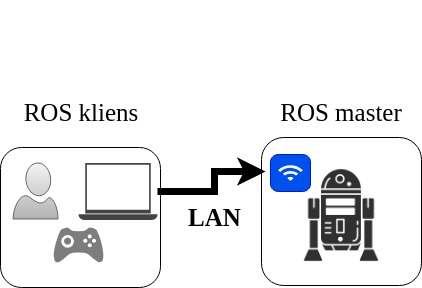
\includegraphics{tikz/RobotUserLan.jpg}
  \caption{Robothoz csatlakozás a Wifi-n keresztül.}
  \label{fig:RobotUserLan}
\end{figure}


Az \ref{fig:ROSgraph} láthatóak a főbb nodok, topikok és a köztük levő relációk. A nodok és a topikok leírását a \ref{Tab:nodok}

\begin{table}[H]
\centering
\begin{tabular}{lp{3cm}p{8cm}}
\hline Node Név & Típus & Leírás \\ \hline
  /R és /L      &  FPGA
  Communication
  Modul     &  Az FPGA-val való kommunikációért felelős. Adatokat fogad/küld  a \ref{FPGAcomuSection} fejezetben leírt protokoll alapján, amelyeket továbbít a ROS operációs rendszerben működő nodoknak.     \\
  /ImuInBoxA       &    Imuxxxx   &  Feladata szöveges formában érkező adatok feldolgozása és a ROS keretrendszerbe integrálását oldja meg. Mért fizikai mennyiségek:       \\
  /WheelOdometry       &       &   Kerekek mozgásából számolt robot elméleti pozíciója a térben     \\
  /TeleopJot      &       & Feladata a joystick-től érkező parancsok fogadása. Megvalósítja a $Dead Man Switch$ gomb kezelését, létrehoz egy globálisan engedélyező jelet a /setEMS-t és a /TeleopSig-t, amely előírja a robot lineáris mozgási sebességét és a forgási sebességét a Z tengely körül.  \\
  /rplidarNode & & A lidar mérési adatait olvassa ki és továbbítja a /scan topikban.\\
  /rosserial\_server & & A megvalósítja a kommunikációt egy esp8266 fejlesztőlap és a ROS között, amely az akkumulátorok feszültségeinek a merését végzi \cite{RosSerial}.\\
  /Joy & & Joystick eszközök integrációját valósítja meg \cite{rosjoy}.\\
  /hector\_mapping & & Lidar mérései alapján 2D térképet készit a környezetről, miközben lokalizálja a robotot ezen a térképen \cite{roshectormap}\\
  /Measurement & & mérésék elvégzésére szolgáló node, amely egy élőre beállított intervallumokban a megadott referencia értékeket küld ki az FPGA ban levő szabályzóknak.\\
  /TelepoController & & Átalakítja a robot sebesség állapotait és kiszámolja nyílt hurokban a szabályzok előírt értékeit. Abban az esetben, ha a /movebase nodot használjuk, ez megoldja a robot pozíció szabályozását a térképen, így a $/cmd_vel$ csomagot csak átalakítja /refVals csomaggá azáltal, hogy azonos oldalon levő kereke ugyanazt a referencia értéket kell követniük.
  
\end{tabular}
 \label{Tab:nodok} 
\end{table}

\subsection{Üzenet típusok (.msg)}
Az alábbi táblázatban láthatjuk a ROS operációs rendszer által szolgáltatott .msg üzenetek kiterjesztését, amelyek lehetővé teszik az FPGA integrációját a ROS környezethez.
\begin{table}[H]
\centering
\begin{tabular}{lllp{6cm}}
\hline \textbf{Üzenet típus}              & \textbf{Értékek}   & \textbf{Erkek típusa} & \textbf{Leírás} \\ \hline
 header                   &     -     &      std\_msgs/Header      &   Minden üzenet tartalmaz egy fejlécet, amely információkat tartalmaz az üzenetről. \\   
                          & seq       &      uint32        &   minden üzenetet egyedileg beazonosító szám     \\
                          & stamp     &      time        &  idő-bélyeg amely a küldés idő-pillanatát tárolja.      \\
                          & frame\_id  &      string        &        \\  \hline
                          
\hline  \multirow{1}{*}{/GlobalEnable}  &   systemIsOk        &    int16          &    
                                                                          =0 - a HLC működik.
                                                                          
                                                                          <>0 -  a HLC nem nem működik      \\    \hline                    
\hline\multirow{4}{*}{/refVals} & names     & string{[}{]} &        \\
                          & ref\_position  & float{[}{]}  & előírt szög pozíció       \\
                          & ref\_velocity & float{[}{]}  &  előírt szög sebesség      \\ 
                          & ref\_effort &    float{[}{]}  &  előírt forgatónyomaték    \\\hline
 \hline \multirow{1}{*}{/setEMS}  &   value        &     int16         &      =0 - Vészleállító aktív.
                                                                          
                                                                       <>0 -  Vészleállító nem aktív  \\     \hline 
\hline\multirow{3}{*}{/joyControll} & vx     & float64 &    A robot X tengely mentén előírt sebessége m/s-ban.    \\
                          & omega  & float64  & előírt szög pozíció   A robot Z tengely körüli forgása \degree/s-ban.    \\
                          & ControlMode & int64  &  Választhatunk a HLC szabályzok típusa vagy a manuális irányítás közül 
                           =0 move\_base szabályzó, =1 manuális irányítás joystick segítségével.\\   \hline                                                                       
\end{tabular}
\end{table}

A \ref{fig:ROSgraph} ábrán láthatjuk a nodok és az üzenetek közti kapcsolatot.

\renewcommand{\img}{SajatRobot/ROS/rosgraph.svg}
\renewcommand{\sources}{*}
\renewcommand{\svg}{svg}
\renewcommand{\aspectratioPic}{1.4}
\renewcommand{\rotationAnglePic}{90}
\renewcommand{\captionn}{ROS graph}
\renewcommand{\figlabel}{ROSgraph}
\begin{kep}
\begin{figure}[H]
\centering
\ifthenelse{\equal{\svg}{*}}
{
    \includegraphics[width=\aspectratioPic\textwidth,angle=\rotationAnglePic]{\img}
}
{
    \includesvg[width=\aspectratioPic\textwidth,angle=\rotationAnglePic]{\img}
}

 \ifthenelse{\equal{\sources}{*}}
    { \captionof{figure}{ \captionn}}
    { \captionof{figure}{ \mand{\mand{\captionn}{Forrás:}}{}} }
  	

\ifthenelse{\equal{\figlabel}{*}}
    {}
    {\label{fig:\figlabel}}%
    
\renewcommand{\figlabel}{*}



\end{figure}
\end{kep}
\renewcommand{\aspectratioPic}{1}
\renewcommand{\rotationAnglePic}{0}
\renewcommand{\svg}{*}


\subsection{FPGA kommunikációs modul ROS oldali integració}

A ROS biztosít a fejlesztőknek egy megoldást, amelyek képesek újonnan létrehozott robot integrálását ROS környezetben \cite{RosSerial}. Előnye hogy gyorsan látványos eredményt érhetünk el, de a működés sebességben és az üzenetek méretében is korlátozott. Ezen hátrányokból kifolyólag sajátos integráció szükséges, amely integrálta az FPGA UART kommunikáció protokollt a ROS keretrendszerben működő más modulokhoz.

A \ref{fig:ROStoUart} diagramon a kommunikáció node technikai megvalósítását láthatjuk. Különálló szál gondoskodik az UART adatok olvasasáról és írásáról. Az üzenetek értelemezését egy külön szál végzi és hívja fel a kiszolgáló függvényeket.
A paraméterek helyes beállításáról a ParamThread szál gondoskodik, paraméterek helyes beállításáról FPGA oldalon. Abban az esetben, ha a hardver kap egy űj paramétert a \ref{fig:MicroblazeSoft} alapján az FPGA visszaküldi a kapott paramétert, a visszajelzésből eldönthető, hogy a paraméter  a hardverben helyesen állítódott e be. Abban az esetben, ha nem megfelelő, újraküldődik mindaddig amíg nem sikeres a beállítás.

A paraméterek kezelésére a ROS paraméter szerver a felelős \cite{parameterserver}, abban az esetben, ha egy paraméter megváltozott, amely az illető nodehoz köthető, akkor a \ref{fig:ROStoUart} ábrán látható ParameterValtozott esemény előidézi a  megváltozott paraméter értékének az elküldését  FPGAnak irányába.

A globális engedélyező jel a \ref{fig:ROStoUart} MasterLive Enable,  /globalEnable típusú üzenettel engedélyezhetjük a szabályzok működését, a folyamatos működéshez 500ms periódussal kell érkeznie. Abban az esetben, ha a központi számítógép valami okból leállna, akkor a hardveres szabályzok is leállnak. A node 300ms periódussal küldi tovább az engedélyező jelet az FPGA modulnak. A HardverLive jel információt szolgáltat a többi ROS környezetben futó és a működés szempontjából kritikus nodenak, hogy az adott modul megfelelően működik e. Ezen információ birtokában a HeartBeat node leállítja a rendszert, ha egyik FPGA modul nem válaszol.

\renewcommand{\img}{SajatRobot/ROS/NodeUML.jpg}
\renewcommand{\sources}{*}
\renewcommand{\captionn}{ROS integrálása Uart protokolhoz.}
\renewcommand{\figlabel}{ROStoUart}
\begin{kep}
\begin{figure}[H]
\centering
\ifthenelse{\equal{\svg}{*}}
{
    \includegraphics[width=\aspectratioPic\textwidth,angle=\rotationAnglePic]{\img}
}
{
    \includesvg[width=\aspectratioPic\textwidth,angle=\rotationAnglePic]{\img}
}

 \ifthenelse{\equal{\sources}{*}}
    { \captionof{figure}{ \captionn}}
    { \captionof{figure}{ \mand{\mand{\captionn}{Forrás:}}{}} }
  	

\ifthenelse{\equal{\figlabel}{*}}
    {}
    {\label{fig:\figlabel}}%
    
\renewcommand{\figlabel}{*}



\end{figure}
\end{kep}
\renewcommand{\aspectratioPic}{1}
\renewcommand{\rotationAnglePic}{0}
\renewcommand{\svg}{*}


\subsection{Előirt értékek}
A /refVals típusú üzenetben megadjuk minden egyes motor előírt értékét annak fövenyében $\degree/s$ hogy sebesség alapján szabályzunk vagy $N/m$ előírt nyomaték alapján.


\subsection{Vonatkoztatási Rendszerek }
A  vonatkoztatási rendszerek szükségesek, mert a szenzorok és beavatkozó eszközök egymáshoz viszonyított helyzete és poziciója is változhat. Sok esetben szükséges ismernünk egy adott eszköznek a múltbeli helyzetét, vagy egy másik vonatkoztatási rendszerhez képest a pozícióját vagy irányát. A ROS biztosít egy tf \cite{rosTF} nevű csomagot amely megvalósítja a szűkséges transzformálásokat a $VNR$-k között. 
A \ref{fig:ROSframes} látható a kialakított vonatkoztatási rendszerek a roboton amely hűen modellezi a fizikai robot kialakítását.
A vonatkoztatási rendszereket két csoportba oszthatók:

\begin{enumerate}[label=(\alph*)]
\item rögzített pozíció és szögek, szabadságok 0:
Szenzorok laser, BODY\_link, wheel\_odom, ImuALink VNR je a base\_link a globális robot VNR hoz:
\item rögzített pozíció csak szögek változnak, szabadságok 1: Kerekek VNR je: FL\_link, BL\_link, FR\_link, BR\_link a BODY\_link hez képest csak Y körül foroghat.
\item pozíció és szög is változik, szabadságok 6:
A robot base\_link az helymeghatározás odom, és az odometria a térképhez map viszonyítva.
\end{enumerate}


A robot modellt ROS környezetben URDF robot leíró, xml alapú fájlal tehetjük meg, \cite{rosURDF}
\cite{rosJoint} \cite{rosLink}.
Az <origin> tag az xzy paraméter alatt, megadhatjuk a csukló pozícióját mindhárom tengelyen, méterben kifejezve a <parent> tagban szereplő linkhez képest. Az rpy paraméter alatt az elfordulásokat rendre x, y, z tengelyek mentén radiánban kifejezve.
Az <axis> tagban beállíthatjuk a kényszereket, jelen esetben csak az y tengely körüli forgás engedélyezett, azaz a kerekek esetében. 
Az <link> tagban robot elemeket hozhatunk létre. Az alábbi XML-ben látható a robot fizikai leírása, amely megfelel a valós szerkezetnek.
\begin{lstlisting}[language=XML]
<robot name="mobile_robot_platform_4Wheel">
	<link name="base_link" > </link>
	<link name="FL_link" > </link>
	<link name="BR_link" > </link>
	<link name="BL_link" > </link>
	<link name="BODY_link"> </link>  
	<link name="ImuALink"> </link>  
	<link name="laser"> </link> 

	<joint name="FL" type="continuous">
		<parent link="BODY_link"/>
		<child link="FL_link"/>    
		<origin xyz="0.29 -0.33 0" rpy="0 0 0" />
		<axis xyz="0 1 0" />
	</joint>

	<joint name="FR" type="continuous">
		<parent link="BODY_link"/>
		<child link="FR_link"/>    
		<origin xyz="0.29 0.330 0" rpy="0 0 0" />
		<axis xyz="0 1 0" />
	</joint>

	<joint name="BL" type="continuous">
		<parent link="BODY_link"/>
		<child link="BL_link"/>
		<origin xyz="-0.29 -0.330 0" rpy="0 0 0" />
		<axis xyz="0 1 0" />
	</joint>

	<joint name="BR" type="continuous">
		<parent link="BODY_link"/>
		<child link="BR_link"/>     
		<origin xyz="-0.29 0.330 0" rpy="0 0 0" />
		<axis xyz="0 1 0"/>
	</joint>

	<joint name="imuAandGPS" type="fixed">
		<parent link="base_link"/>
		<child link="ImuALink"/>
		<origin xyz="0.125 0.03 0.11" rpy="0 0 0" />
	</joint>

	<joint name="laserAJoin" type="fixed">
		<parent link="base_link"/>
		<child link="laser"/>
		<origin xyz="0.39 -0.02 0.23" rpy="0 0 3.14" />
	</joint>  

	<joint name="contact" type="fixed">
		<parent link="base_link"/>
		<child link="BODY_link"/>
	</joint> 
</robot>
\end{lstlisting}

A \ref{fig:ROSframes} láthatjuk, hogy a robot törzsét a $BODY\_link$ alkotja, amelyhez kapcsolódnak a kerekek: $BL\_link,FL\_link,BR\_link,FR\_link$. A $base\_link$ és a $BODY\_link$ egybe esnek. A szenzorok a $laser$, amely a lidarnak felel meg, $ImuALink$ IMU szenzor ezek a $base\_link$-hez kapcsolódnak.
A $map$ VNR a térképnek, amelyen meghatározzuk a robot pozícióját $odom$.

\renewcommand{\img}{SajatRobot/ROS/frames.svg}
\renewcommand{\sources}{*}
\renewcommand{\svg}{svg}
\renewcommand{\aspectratioPic}{1.5}
\renewcommand{\rotationAnglePic}{90}
\renewcommand{\captionn}{A megvalósított robot VNR-k közti reláció }
\renewcommand{\figlabel}{ROSframes}
\begin{kep}
\begin{figure}[H]
\centering
\ifthenelse{\equal{\svg}{*}}
{
    \includegraphics[width=\aspectratioPic\textwidth,angle=\rotationAnglePic]{\img}
}
{
    \includesvg[width=\aspectratioPic\textwidth,angle=\rotationAnglePic]{\img}
}

 \ifthenelse{\equal{\sources}{*}}
    { \captionof{figure}{ \captionn}}
    { \captionof{figure}{ \mand{\mand{\captionn}{Forrás:}}{}} }
  	

\ifthenelse{\equal{\figlabel}{*}}
    {}
    {\label{fig:\figlabel}}%
    
\renewcommand{\figlabel}{*}



\end{figure}
\end{kep}
\renewcommand{\aspectratioPic}{1}
\renewcommand{\rotationAnglePic}{0}
\renewcommand{\svg}{*}



\section{Kerekek Pid Szabalyzo hangolas}

A pid, a legelterjedtebb szabályozó egyszerű feladatok elvégzésére, esetünkben is elegendő a kerekek szögsebesség szabályzására kerekenkénti egy PID szabályzóval. A PID szoftveresen fut a uBlaze processzoron. Bemenete egy előírt forgási sebesség \degree/s ban és kimenete egy -32000 és 32000 egész típusú értek. A kimenti érteke a PWM kitöltési tényezőt jeleni, az előjel pedig a beavatkozás irányát.
Matlab/Simulink környezetben használva a Robotix Toolbox segítségével direkben pwm beavatkozo referenica erteket irtam elo a motroknak. A beavatkozó jel előállítása és elküldési a fizikai eszköznek 0-100\%-ig 10\% lépcsőkben amelyek 0\% kitoltesekkel vanak megszakitva. A mert adatokat rosbag csomagba mentve majd a System Identification Toolbox használatával identifikáljuk a rendszer modellt. A rendszer bemenete egy beavatkozójel ami fizikailag feszültségnek fele meg 0V és 12V között. A kimenetek a forgási sebesseg.
A mert adatokat Matlab/System Identification hasznalataval megbecsuljuk a rendszer modeleket. Nemlinearis modelt becslunk 
Hammerstein-Wiener model \cite{matlabhwmmodel} hasznalva, 1 kimenet es 1 bemenet, a linearis atviteli fugveny fokszama:
zerusok nb = 2, polusok nf = 3, keses a bemenet es a kimenet kozott nk = 1. A becsult adatok 94\% ban megfelelnek a mert rendszernek.          

A mereseket a robot kerekei es a talaj erintekzese nelkul vegeztem.
A becsult modelt a bemenet 50/\%  korul linearizaljuk es a linearizalt modelbol atviteli fugvenyt kesztunk. 
$tf = tf(linearize(model,16000));$ utasutast hasznalva Matlab kornyezetben. A linearizalt modelt Matlab/PidTuning eszkozt hasznalva behangolunk kiszamitjuk a megfelelo PID szabalyzo parametereit.

\input{SajatRobot/PIDHangolasa/MeasuremetSimulinkWheel.tex}

A becsült rendszer átviteli függvénye $H_s(z)$, mintavetelezesi periódus Ts: = 0.05s.

\subsection*{Nagyobik fokozatban}

A becsult modelt oszehasonlitva a mert ertekekkel a \ref{fig:NFsysIdent}, a model nemlinearis becsult model megfelel a mert ertekeknek.

\begin{figure}[H]
  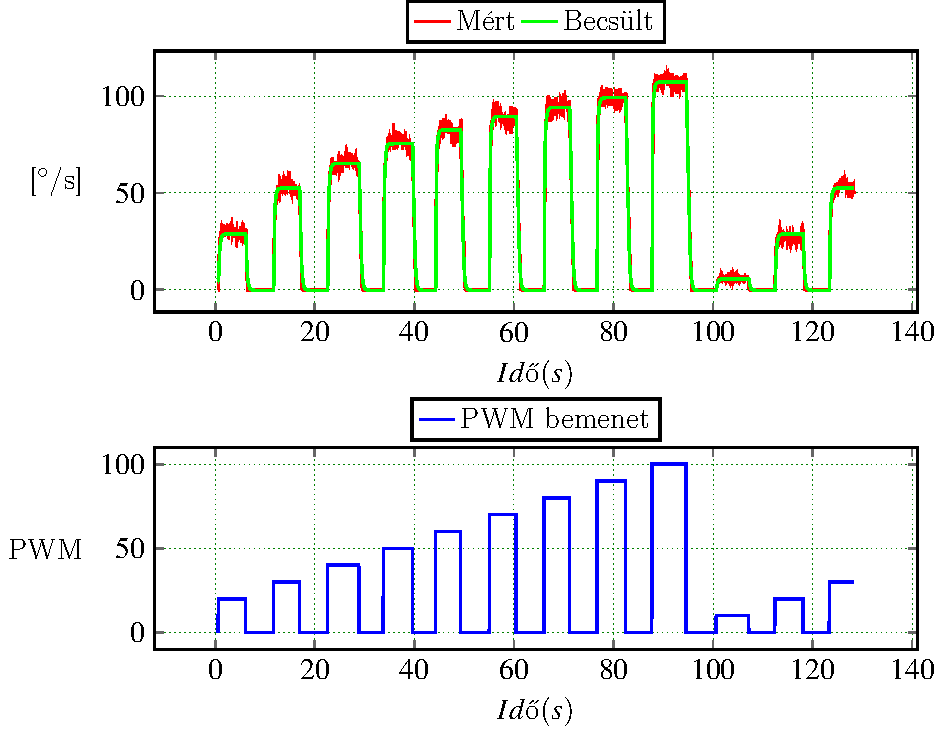
\includegraphics{tikz/NFsysIdent.pdf}
  \caption{Nagy fokozat Hammerstein-Wiener becsult model valasza, es a mert ertekek.}
  \label{fig:NFsysIdent}
\end{figure}


Az atviteli fuggveny a bemenet 50/\% korul linearizalva.

\begin{equation}
    H_s(z)=\frac{-0.07017z^{-2} -0.053z^{-1}}{-0.2117^{-3}+0.7321z^{-2} -1.393z^{-1} +1}
\end{equation}

A tervezett PID szabályozó paramétere Kp: 7.11 , Ti: 23.66 , Td: 0.43

\subsection{Kisebik fokozatban}

A becsult modelt oszehasonlitva a mert ertekekkel a \ref{fig:KFsysIdent}, a model nemlinearis becsult model megfelel a mert ertekeknek.


\begin{figure}[H]
  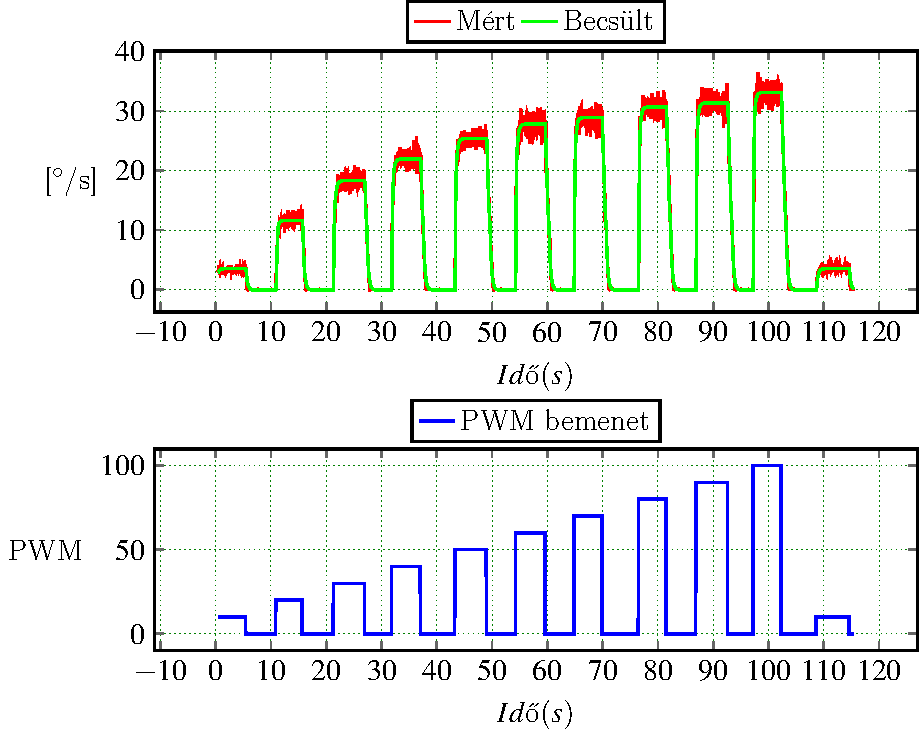
\includegraphics{tikz/KFsysIdent.pdf}
  \caption{Kis fokozat Hammerstein-Wiener becsult model valasza, es a mert ertekek.}
  \label{fig:KFsysIdent}
\end{figure}

Az atviteli fuggveny a bemenet 50/\% korul linearizalva.

\begin{equation}
    H_s(z)=\frac{-0.0291z^{-2} -0.009263z^{-1}}{-0.198z^{-3}+0.7058z^{-2} -1.394z^{-1} +1}
\end{equation}

A tervezett PID szabályozó paraméterek: Kp: 15.96 , Ti:51.51 , Td:1.237 

.



\newpage
\section{Pályakövetési feladatok}

A robot pályakövetési feladatát megfogalmazhatjuk úgy, hogy tudjunk eljutni A pontból B pontba, ha ismerjük a robot síkbeli pozícióját és az orientációját egy térképen, amely megfelel a környezetnek, látható az \ref{fig:PositionController} ábrán.
A \ref{fig:PositionController} ábrán látható, hogy felveszünk egy pozitív és egy negatív irányt a szögre nézve, az orientációkat mindig [0\degree 360\degree] között kell megadjuk. A robotnak mindig arra kell fordulnia, amerre a szög a legkisebb, azért, hogy minél kevesebbet keljen mozogjon.
A kiinduló állapotban a robot kezdetben az A pontban van és az orientációja $\beta_0$ és a B pontba szeretnénk eljutni egyenes vonalban. Így a robotnak kezdetben a célra kell fordulnia és ezután haladhat előre, miközben korrigálja az orientációs hibákat.
Első lépésben a robotnak fordulnia kell $error$ szöget, hogy $\beta_1$ irányba mutasson és ezután haladhat a cél fele.


\begin{figure}[H]
    		%trim = bal also jobb felso
   \fbox{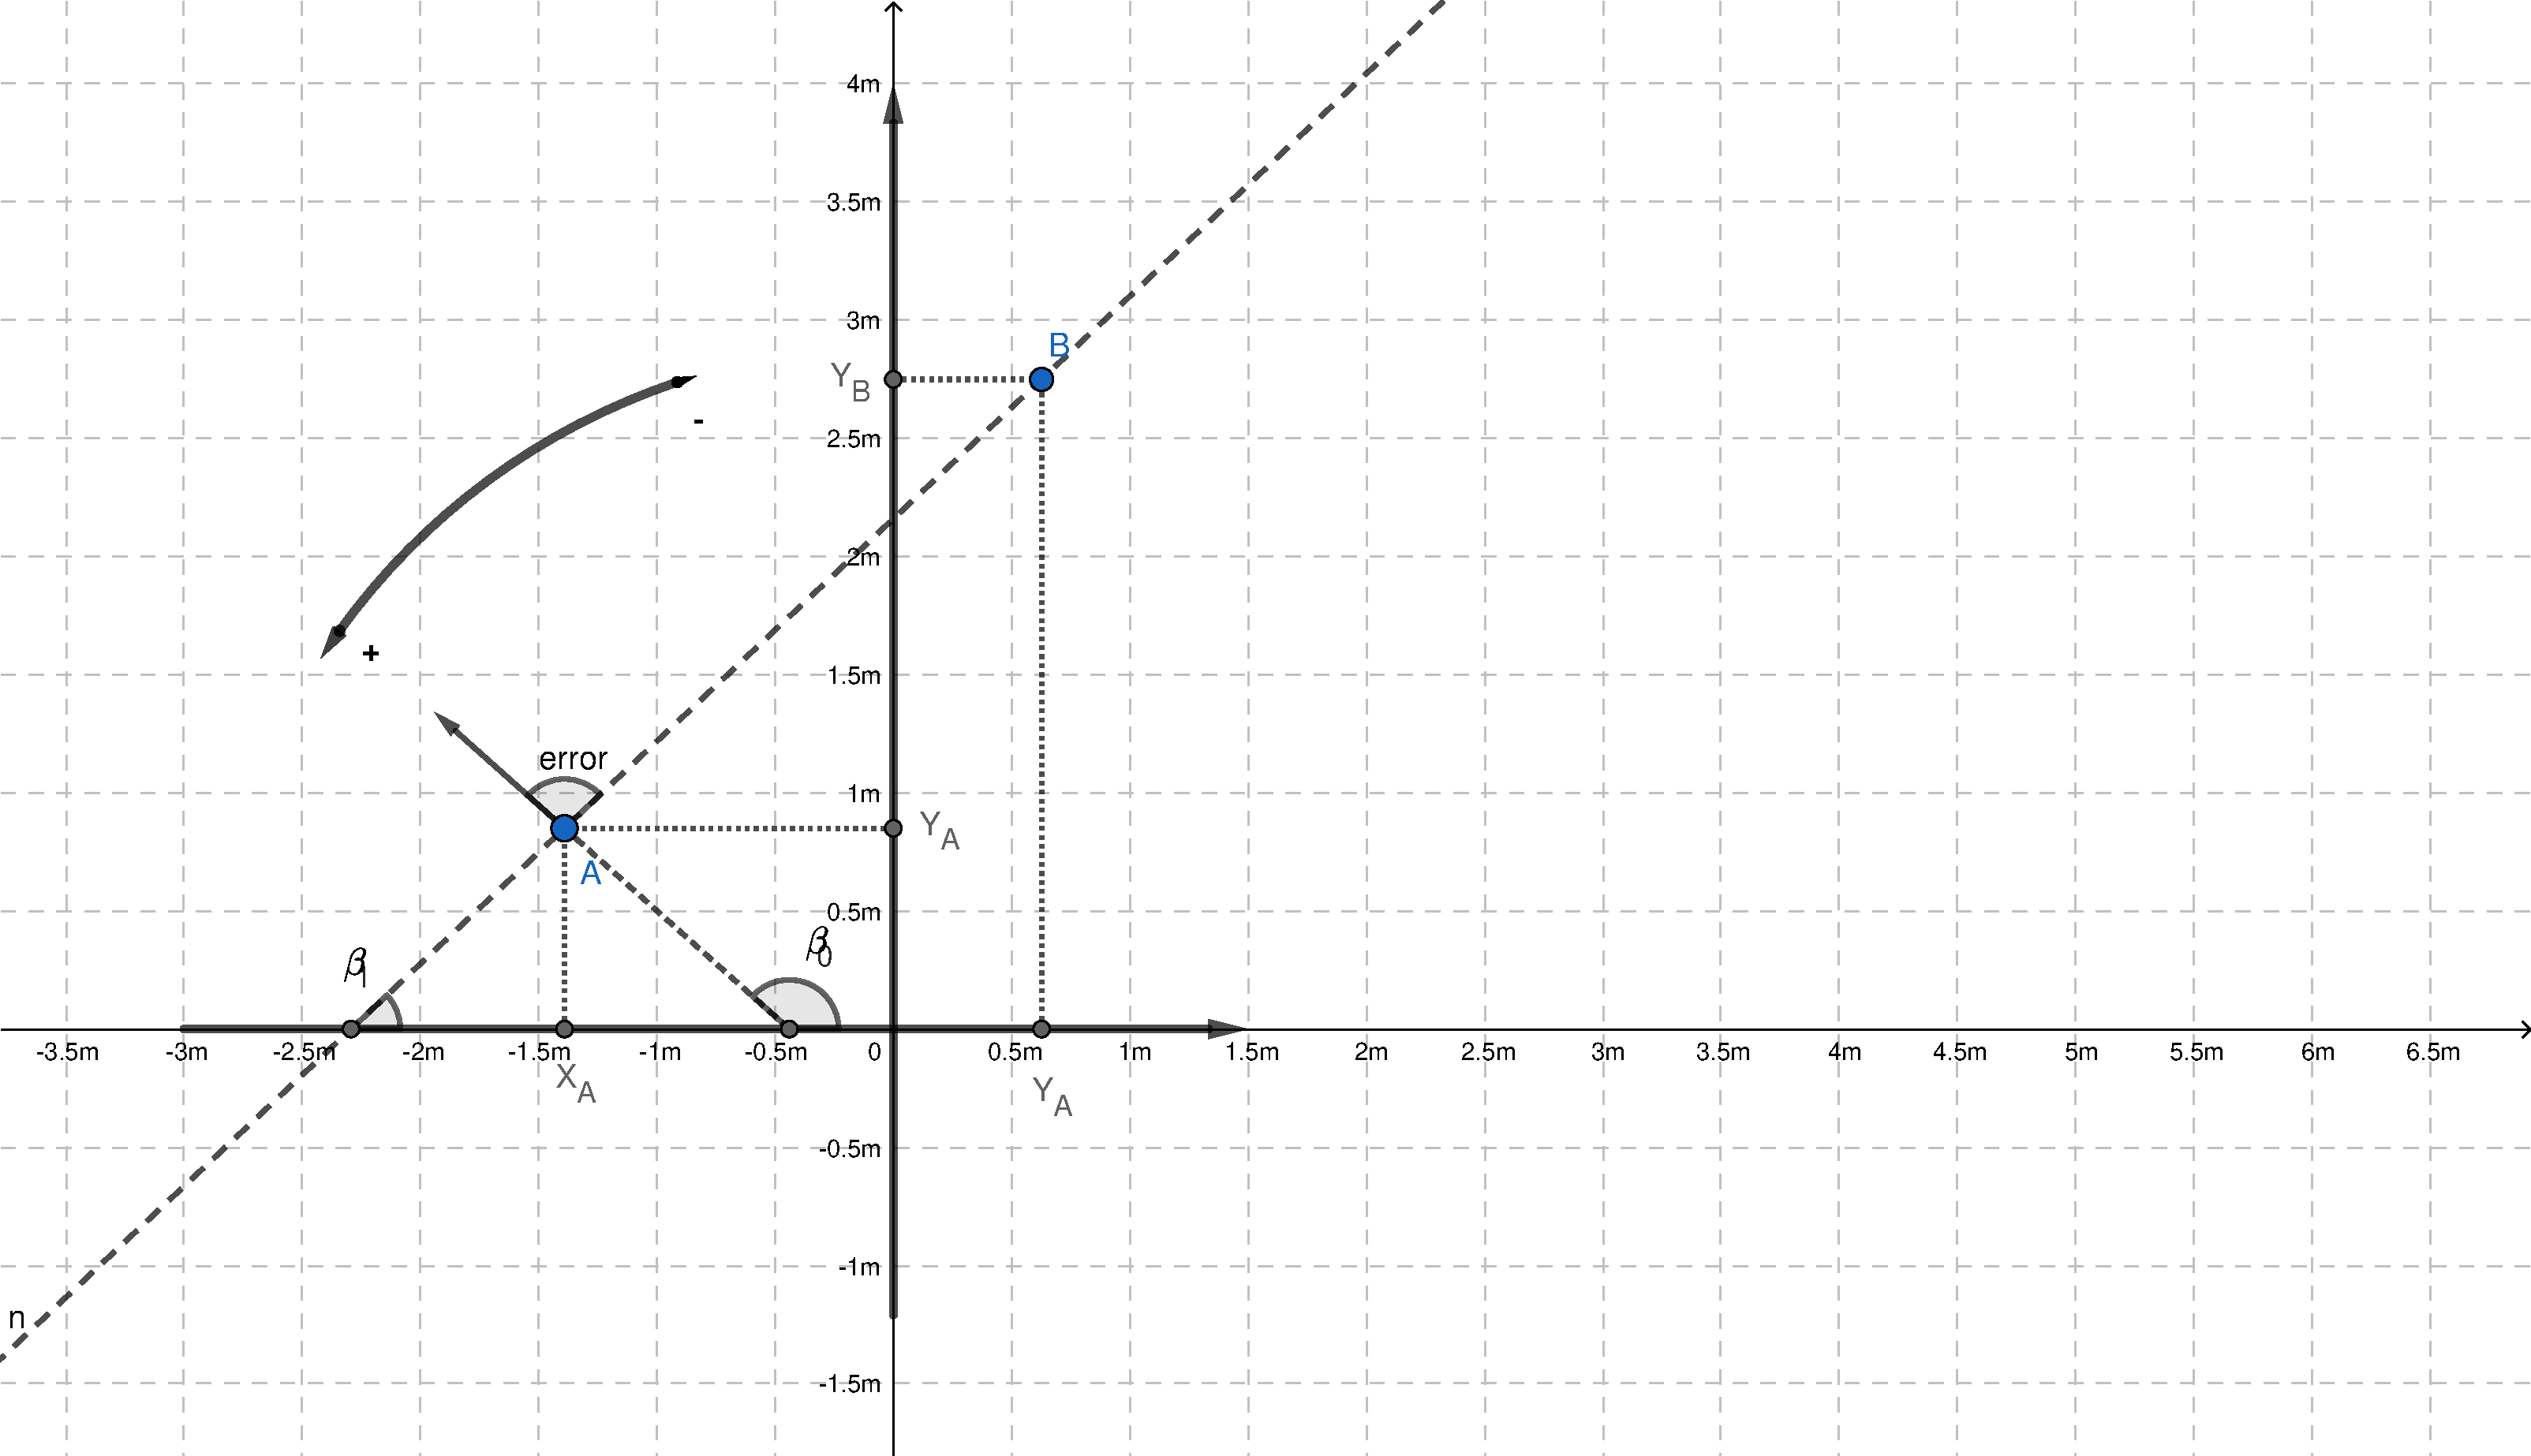
\includegraphics[width=1\columnwidth,trim=3cm 6cm 27cm 2cm,clip]{tikz/PositionController.pdf}}
  \caption{Robot pozíció szabályzása}
  \label{fig:PositionController}
\end{figure}


A pályakövetési algoritmus látható alább. Az  előírt irányt $tan^{-1}$ függvény segítségével határozzuk meg, ismerve X és Y tengelyen a hibák nagyságát. A Rotate($e_\alpha$,$\Omega_{max}$) függvényben alkalmazunk egy PI típusú szabályzót, melynek a feladata a szöghiba 0-hoz való közelítése. A Vx(d,$V_max$) a robot lineáris sebességének a szabályzását látja el egy PI típusú szabályzó, célja a robot és a kitűzött cél távolságának a csökkentése. 
A távolságszabályzó bemenetét súlyozzuk $1/e_\alpha$ értékkel, hogy ameddig nincs a robot irányban, addig ne domináljon távolságszabályzó.

\begin{algorithm}
   \caption{Pályakövetés Algoritmusa}
    \begin{algorithmic}[1]
     %\Function{GetNextControl}{$X_a,Y_a\alpha$}
      \Function{GetNextControl}{$X_a,Y_a,\alpha_a,X_t,Y_t,\alpha_t,Tr,Tr_\alpha,\Omega_{max},V_{max}$}
      %\Comment{Ahol X,Y - pozicio a térképén, \alpha irány, a - aktuális, t - előírt, Tr - pozicio hiba küszöb, $Tr_{\alpha}$ - szöghiba küszöb,${\Omega}_{max}$ maximális forgási sebesseg, $V_{max}$ maximális haladási sebesség. }
      
       \State $e_x = X_a-X_t$
       \State $e_y = Y_a-Y_t$
       \State $d=\sqrt{e_x^2+e_y^2}$
       \State $\alpha_i=dir(X_a,Y_a,X_t,Y_t)$ \Comment{Két ponton átmenő egyenes iránytényezője}
       \State $e_\alpha=\alpha_i-\alpha_a$
            \If {$e_\alpha > Tr_\alpha$} \Comment{Fordulj a cél fele}
                \State $\Omega = Rotate(e_\alpha,\Omega_{max}) $
                \State $V_x = 0 $
            \Else \Comment{Haladj a cél fele és korrigáld az elfordulást}
                
                \State $\Omega = Rotate(e_\alpha,\Omega_{max}) $
                \State $V_x = Vx(d*1/e_\alpha,V_{max})$
            \EndIf
     
            \If {$e_\alpha < Tr_\alpha$ és $d<Tr$} \Comment{Kívánt pozícióban}
                \State $\Omega = 0$
                \State $V_x = 0 $
            \EndIf
        
       \EndFunction

\end{algorithmic}
\end{algorithm}



Az algoritmus tesztelésére MATLAB/Simulink környezetet használtam. A robot kinematikai modellt az \ref{eq:allapot} egyenlet alapján modelleztem, a pozíciók (X,Y) és az irány meghatározására integráltam a lineáris és szögsebességeket. 

A \ref{fig:SimPoseCont} ábrán láthatjuk a szimulációs eredményeket, amint a robot egy végtelen jelhez hasonló pályát követ.

\begin{figure}[H]
	\setlength{\fboxsep}{0pt}
	\setlength{\fboxrule}{0pt}
	
    \begin{center}  	
    		%trim = bal also jobb felso
    	\fbox{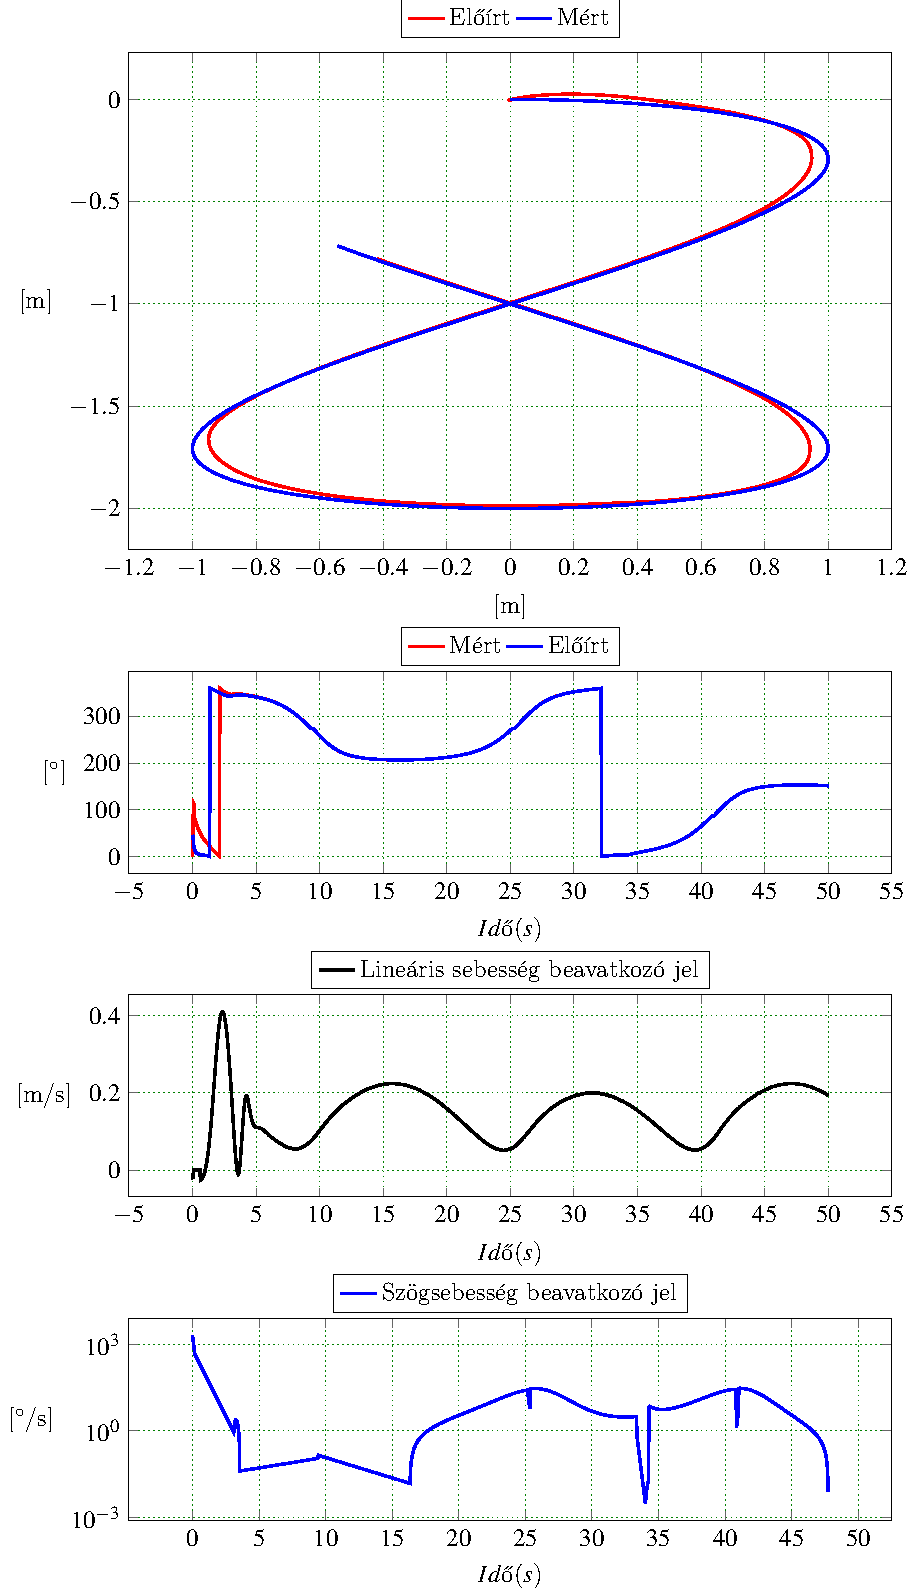
\includegraphics[width=0.9\columnwidth,trim=0cm 0cm 0cm 0cm,clip]{tikz/SimPoseCont.pdf}}
    \end{center}  
    
  	\caption{Robot pozíció szabályzása}
  	\label{fig:SimPoseCont}
\end{figure}



\lhead{Meresek a Robottal}
\section{Meresek}
Ebben a fejezetben tanulmányozásra kerül a robot viselkedése abban az estekben ha valamely kerék meghibásodik, és ezáltal nem megfelelően működik.
Hasonló eset történt a Marson a Spitit mars roverrel (2006,Március,13) \cite{SpititWheel1} amikor az első jobb kereke meghibásodott. A megoldás az volt hogy a robot mozgása optimálisabb lesz energia felhasználás szempontjából ha háttal megy. Az energia ellátása is véges volt, kiszolgáltatott volt a napsütésnek,a nap elemekre rakodót por miatt csökkentek a ayok hatásfoka így sokkal alaposabb mozgás pálya tervezésre volt szükség.
Problémák adódtak a homokos talajjal is, a Spirit mars járonak, kerekei a homokba süllyedtek és beragadtak, a földi irányító csoport egy másolat segítségével próbálta kimozdítani a csapdaból.
A hasonló eseteket elkerülhetők lennének, ha ismerve a robot korlátait olyan mozgás pályát határoznak meg amellyel elkerulhetjuek ezen akadajokat, vagy időben detektálhatjuk ezen problémákat pl: homokba süllyedés érzékelése.


A robottal a következő méréseket fogjuk elvégezni:
\begin{enumerate}[label=(\alph*)]
\item BL kerék blokált
\item BL és BR kerék blokált
\item BL kerék maximálisan pörög
\item BL és BR kerék maximálisan pörög
\end{enumerate}


\subsection{Differenciális Forgás Vízszintes Talajon}

Diferencialis forgasnak nevezuk azt amikor a jobb es ball oldali kerekek sebesege megegyezo, csak iranyukban elenkezo, igy a robot belso teruleten belul jon letre a ICR pont a COG kozeleben kelene legyen \ref{fig:SMR4WKinematics}. 


%%globalis paremeterek a meresek kirajzolasahoz.

\pgfplotstableset{%
    x index=0,
    y index=1,
    header=true
}%

\pgfplotsset{every axis/.append style=
    {
        font=\large,
        line width=1.2pt,
        tick style={line width=0.8pt}
    }
}

\pgfplotsset{
    contour/every contour label/.style={
    sloped,
    transform shape,
    inner sep=1pt,
    every node/.style={mapped color!50!black,fill=white},
    /pgf/number format/relative={\pgfplotspointmetarangeexponent},
    },
}






\subsection{Feloldali kerekek blokolva kavicsos talajon}

A robot baloldali kerekei leblokkolva és a jobboldali kerekei 50\degree/s szögsebességgel forognak. Az eredmények alapján a \ref{fig:Left0Right50b} látható a robot által leírt pálya. A mozgás során több mint 360 \degree -t fordul és mondhatni körpályát írt le. A talajjal való súrlódások miatt a robot nem tökéletesen fordul ez látható abból is hogy a másodszori fordulás már az előzőhöz képest más középponttal rendelkezik. 

\renewcommand{\GlobalPath}{Meresek/Mozgasok/HibasMukodes/R_0_L_1/}
\renewcommand{\secondImage}{*}

%kep a talajrol
%

\renewcommand{\sources}{}
\renewcommand{\captionn}{Kep a felszinrol}
\renewcommand{\figlabel}{figm}


\begin{kep}
    \begin{figure}[H]%
    \begin{center}
    
    \subfloat[label a]{
        {\includegraphics[width=9cm]{\mand{\GlobalPath}{talaj1.jpg}} }
        \label{fig:ex3-a}
    }%
    
    \ifthenelse{\equal{\secondImage}{*}}
    {}
    {
        \qquad
        \subfloat[label b]{{\includegraphics[width=9cm]{\mand{\GlobalPath}{talaj1.jpg}} }}%
    }
  
    \label{fig:example}%
    \end{center}
\end{figure}
\end{kep}

\renewcommand{\secondImage}{*}



%1
% %1
    \begin{figure}
    
        %-------------------------------------------------Joint Adatok---------------
        \begin{subfigure}{\textwidth}
            \begin{center}
        
            \input{\mand{\GlobalPath}{L.tex}}
            \pgfplotstableread{NodeLeft.dat}{\leftNode}

            
            \input{\mand{\GlobalPath}{R.tex}}
            \pgfplotstableread{NodeRight.dat}{\rightNode}

        
            \begin{tikzpicture}
            \pgfplotsset{every axis plot/.append style={very thick}}
            \setcaptionsubtype
            
            % megjelenites beallitasai
            
            \begin{groupplot}[%
                        ,group style={%
                            ,group name=my plots
                            ,group size=2 by 2
                            ,vertical sep=1.8cm,
                            ,horizontal sep = 2.4cm,
                            ,ylabels at=edge left
                        }
                        ,width=7cm
                        ,height=6cm
                        ,try min ticks=5
                        ,xlabel={\bfseries{\emph{\idoFelirat}}}
                        ,zlabel={\bfseries{\emph{kg}}}
                        %%ha kell y felirat az elso ketore
                        %,ylabel={\bfseries{\degree$/s$}}
                        %,ylabel style={rotate=-90}
                        %,xtick={0,10,...,60},
                        %,minor tick num=5
                        %,xtick distance=10
                        %,ytick distance=25
                        ,grid=major%both
                        ,every both grid/.style={gray, opacity=0.7},
                        view={0}{90},
                        legend columns=2,
                        %xmin=0,xmax=0.65,
                        %ymin=0,ymax=0.65,
                       % zmin=-5,zmax=60,
                        ]
            %% ide jonnek a adatok. 
            
            %ha kell felirat be kell teni a nextplot[] parameterei koze
            % \nextgroupplot[ylabel=\degree$/s$, ylabel style={rotate=-90},legend to name={CommonLegend},legend style={legend columns=2}]
            \nextgroupplot[]
                \addplot [color=green,each nth point={\nth}] table [header=true, x=Time, y=refOmegaA] {\leftNode};\label{plots:plot3}
                \addplot [color=black,each nth point={\nth}] table [header=true, x=Time, y=effortA] {\leftNode};\label{plots:plot4}
                \addplot [color=blue,each nth point={\nth}] table [header=true, x=Time, y=omegaA] {\leftNode}; \label{plots:plot1}
                \addplot [color=red,each nth point={\nth}] table [header=true, x=Time, y=pwmA] {\leftNode};\label{plots:plot2}
                \coordinate (top) at (rel axis cs:0,1);% coordinate at top of the first plot
            
            \nextgroupplot[]
                \addplot [color=green,each nth point={\nth}] table [header=true, x=Time, y=refOmegaA] {\rightNode};
                \addplot [color=black,each nth point={\nth}] table [header=true, x=Time, y=effortA] {\rightNode};
                \addplot [color=blue,each nth point={\nth}] table [header=true, x=Time, y=omegaA] {\rightNode};
                \addplot [color=red,each nth point={\nth}] table [header=true, x=Time, y=pwmA] {\rightNode};
                    
            \nextgroupplot[]
                \addplot [color=green,each nth point={\nth}] table [header=true, x=Time, y=refOmegaB] {\leftNode};
                \addplot [color=black,each nth point={\nth}] table [header=true, x=Time, y=effortB] {\leftNode};
                \addplot [color=blue,each nth point={\nth}] table [header=true, x=Time, y=omegaB] {\leftNode};
                \addplot [color=red,each nth point={\nth}] table [header=true, x=Time, y=pwmB] {\leftNode};
                   
            \nextgroupplot[]
                \addplot [color=green,each nth point={\nth}] table [header=true, x=Time, y=refOmegaB] {\rightNode};
                \addplot [color=black,each nth point={\nth}] table [header=true, x=Time, y=effortB] {\rightNode};
                \addplot [color=blue,each nth point={\nth}] table [header=true, x=Time, y=omegaB] {\rightNode};
                \addplot [color=red,each nth point={\nth}] table [header=true, x=Time, y=pwmB] {\rightNode};
                \coordinate (bot) at (rel axis cs:1,0);% coordinate at bottom of the last plot
            \end{groupplot}
            
            %\path [nodes={anchor=south,rotate=90,font=\large\bfseries,midway}]
            %  (my plots c1r1.outer north west)--(my plots c1r2.outer south west)
            %    node {Testing of Parameters 1}
            %  (my plots c2r1.outer north west)--(my plots c2r2.outer south west)
            %    node {Testing of Parameters 2};
            
            % legend
            \node[text width=.5\linewidth,align=center,anchor=south] at (my plots c1r1.north) {\caption[]{FL\label{subplot:one}}};
            \node[text width=.5\linewidth,align=center,anchor=south] at (my plots c2r1.north) {\caption[]{FR\label{subplot:two}}};
            \node[text width=.5\linewidth,align=center,anchor=south] at (my plots c1r2.north) {\caption[]{BL\label{subplot:three}}};
            \node[text width=.5\linewidth,align=center,anchor=south] at (my plots c2r2.north) {\caption[]{BR\label{subplot:four}}};
            
            %\path (top-|current bounding box.west)-- 
            %      node[anchor=south,rotate=90] {throughput} 
            %      (bot-|current bounding box.west);
            % legend
            \path (top|-current bounding box.north)--
                  coordinate(legendpos)
                  (bot|-current bounding box.north);
            \matrix[
                matrix of nodes,
                anchor=south,
                draw,
                inner sep=0.2em,
                draw
              ]at([yshift=1ex]legendpos)
              {
                \ref{plots:plot1}& Aktualis Szogsebesseg [\degree$/s$]&[5pt]
                \ref{plots:plot2}& PWM [$\%$] &[5pt]
                \ref{plots:plot3}& Eloirt Omega [\degree$/s]$
                \ref{plots:plot4}& Energia $[Watt]$ &[5pt]\\
            };
           % \centering
            \end{tikzpicture}
            \end{center}
        \end{subfigure}
        
        \iffalse
        %-------------------------------------------------Power Adatok---------------
        \newline
        \begin{subfigure}{\textwidth}
        \begin{center}
        \input{\mand{\GlobalPath}{Power.tex}}
        \pgfplotstableread{Power.dat}{\power}
        
        
        \begin{tikzpicture}
        \pgfplotsset{every axis plot/.append style={very thick}}
        \setcaptionsubtype
        
        % megjelenites beallitasai
        
        \begin{groupplot}[%
                    ,group style={%
                        ,group name=my plots
                        ,group size=1 by 1
                        ,vertical sep=2cm,
                        ,horizontal sep = 0cm,
                        ,ylabels at=edge left
                    }
                    ,width=14.5cm
                    ,height=6cm
                    ,try min ticks=5
                    ,xlabel={\bfseries{\emph{\idoFelirat}}}
                    %,ylabel={\bfseries{\emph{A}}}
                    %,zlabel={\bfseries{\emph{kg}}}
                    ,grid=both
                    ,every both grid/.style={gray, opacity=0.5}
                    ,view={0}{90},
                    %,xtick distance=10
                    %,minor tick num=5
                    %,ytick distance=5
                    %xmin=0,xmax=0.65,
                    %ymin=0,ymax=0.65,
                    %zmin=-5,zmax=60,
                    ]
        %% ide jonnek a adatok.            
                    
        \nextgroupplot[ylabel=\emph{}, ylabel style={rotate=-90}]
         \addplot [color=red,each nth point={\nth}] table [header=true, x=Time, y=voltage] {\power};\label{plots:plot11}
         \addplot [color=green,each nth point={\nth}] table [header=true, x=Time, y=current]{\power};\label{plots:plot12}
         \addplot [color=black,each nth point={\nth}] table [header=true, x=Time, y=power] {\power};\label{plots:plot13}
        \end{groupplot}
        
        %\path [nodes={anchor=south,rotate=90,font=\large\bfseries,midway}]
        %  (my plots c1r1.outer north west)--(my plots c1r2.outer south west)
        %    node {Testing of Parameters 1}
        %  (my plots c2r1.outer north west)--(my plots c2r2.outer south west)
        %    node {Testing of Parameters 2};
        
        % legend
        \node[text width=.5\linewidth,align=center,anchor=south] at (my plots c1r1.north) {\caption[]{Energia Fogyasztas\label{subplot:one}}};
        
        %\path (top-|current bounding box.west)-- 
            %      node[anchor=south,rotate=90] {throughput} 
            %      (bot-|current bounding box.west);
            % legend
            \path (top|-current bounding box.north)--
                  coordinate(legendpos)
                  (bot|-current bounding box.north);
            \matrix[
                matrix of nodes,
                anchor=south,
                draw,
                inner sep=0.2em,
                draw
              ]at([yshift=1ex]legendpos)
              {
                \ref{plots:plot11}&  Akumlator Feszultsege [V]&[5pt]
                \ref{plots:plot12}& Akkumlator Arama [A] &[5pt]
                \ref{plots:plot13}& Teljesitmeny [W] \\
            };
        
        %\centering
        \end{tikzpicture}
        \end{center}
        \end{subfigure}
        % Caption
        %\caption[]{$SSMR-4W$ tipusu robot kereknyomoerok kerekenkeni változása a sulypont fuggvenyeben}\label{abserror}
        \fi
    \end{figure}




\begin{figure}[H]
	\begin{center}
  		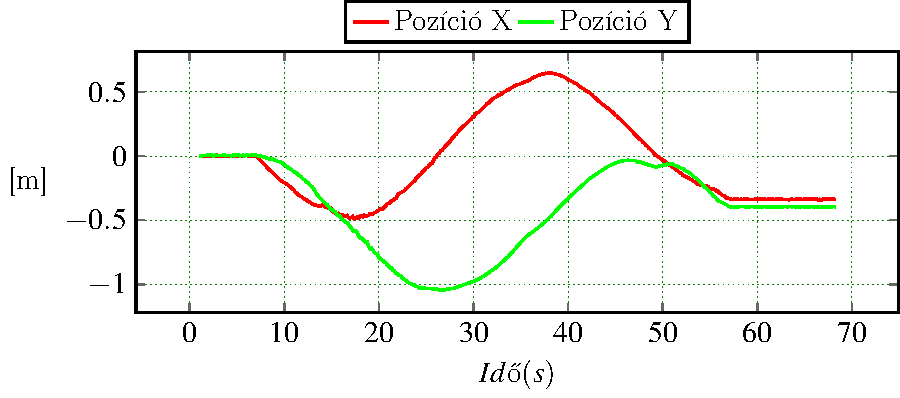
\includegraphics[scale=0.8]{tikz/Left0Right50a.pdf}
  	\end{center}
  \caption{$SSMR-4W$ típusú robot pozíciója, X és Y tengelyekre bontva, keréksebességek BL=FL=0 és a FR=BR= 50\degree/s}
    \label{fig:Left0Right50a}
\end{figure}


\begin{figure}[H]
	\begin{center}
  		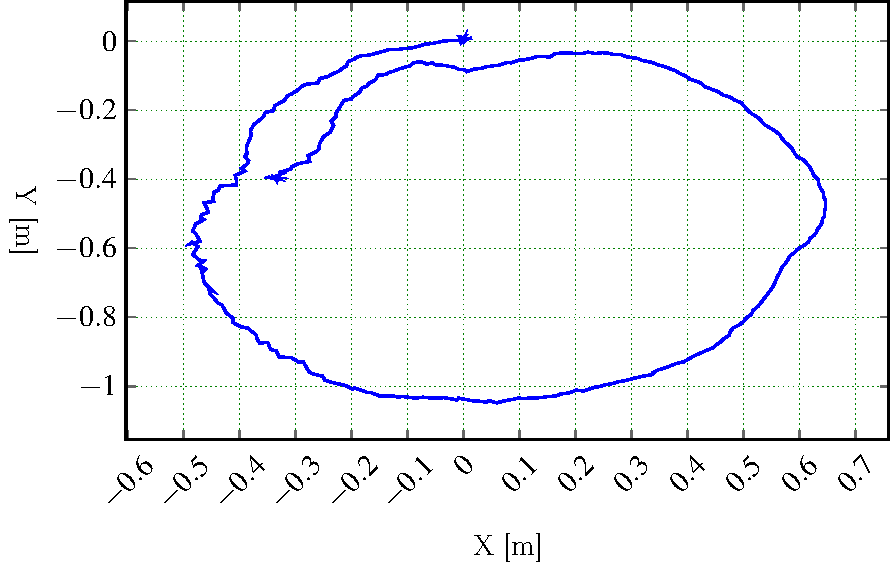
\includegraphics[scale=1]{tikz/Left0Right50b.pdf}
  	\end{center}
  \caption{$SSMR-4W$ típusú robot által leírt pálya, kerekesebességek BL=FL=0 és a FR=BR= 50\degree/s}
  \renewcommand{\figlabel}{Left0Right50b}
  \label{fig:Left0Right50b}
\end{figure}

A mérés során a fordulási szögsebesség 9\degree/s látható a \ref{fig:Left0Right50c} ábran. A LIDAR és HectorMap segítségével mért abszolut szögsebesség zajosabb mint a giroszkóp által mért. A LIDAR-al mért szögsebesség előnyösebb mert a zajokat nem kell integrálni ahhoz hogy megkapjuk a szögsebességet a giroszkóppal ellentétben.

A lineáris sebességeket tekintve \ref{fig:Left0Right50d} szinuszosan változnak, az X és Y tengelyeken, megfigyelhető egy 90\degree eltolódás az X és Y tengelyeken mért szinuszos mozgásban. A kerületi sebesség 0.1 m/s körül adható meg.

\begin{figure}[H]
	\begin{center}
  		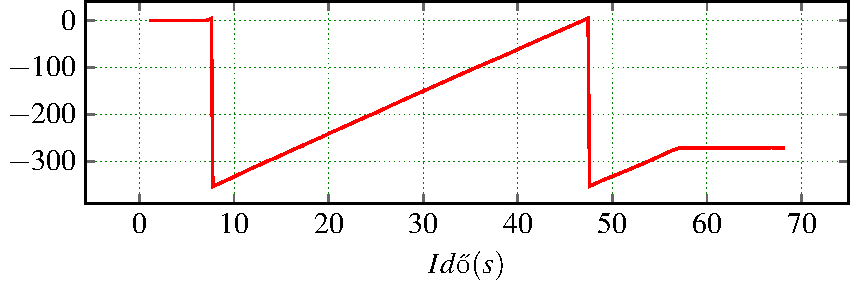
\includegraphics[scale=1]{tikz/Left0Right50c.pdf}
  	\end{center}
  \caption{$SSMR-4W$ típusú robot orientációja,ha a kerékszögsebességek BL=FL=0 és a FR=BR=50\degree/s}
  \label{fig:Left0Right50c}
\end{figure}


\begin{figure}[H]
	\begin{center}
  		\label{fig:Left0Right50d}
  		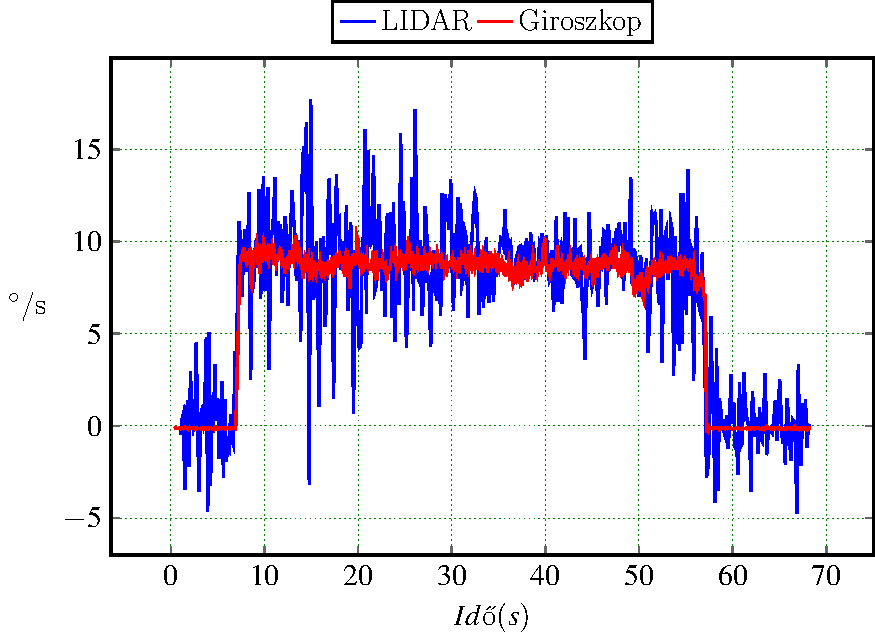
\includegraphics[scale=0.9]{tikz/Left0Right50d.pdf}
  	\end{center}
  \caption{$SSMR-4W$ típusú robot fordulási szögsebessége Giroszkóp és LIDAR által mért értékek, ha a kerékszögsebességek BL=FL=0 és a FR=BR= 50\degree/s}
  \label{fig:Left0Right50d}
\end{figure}


\begin{figure}[H]
	\begin{center}
  		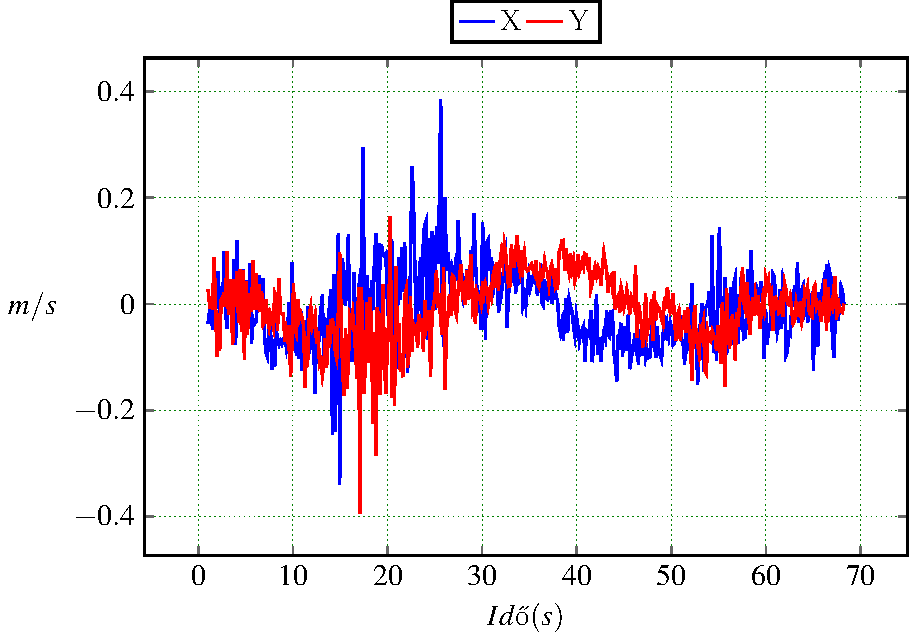
\includegraphics[scale=0.9]{tikz/Left0Right50e.pdf}
    \end{center}
  \caption{$SSMR-4W$ típusú robot súlypontjának sebessége a globális VNR-ben, X és Y tengelyekre bontva, ha a kerékszögsebességek BL=FL=0 és a FR=BR= 50\degree/s}
  \label{fig:Left0Right50e}  
\end{figure}











\subsection{Kavicsos talajon helyben forgás}
A \ref{fig:Left_n50Right50a} megfigyelhető amint a robot kavicsos talajon differenciálisan fordul 60 másodpercen keresztül, ezalatt háromszor teljen korbefordul. A palyat tekintve letrejon egy oldaliranyu mozgás is igy 0.4m kerul odebb. Az oldaliranyu mozgas a nem egyenlo surlodasok es eroeloszlasok miatt jon letre.

\renewcommand{\nth}{2}
\renewcommand{\GlobalPath}{Meresek/Mozgasok/NormalMukodes/DiferencialisanHelybeKavicsos/}
\renewcommand{\secondImage}{*}



\begin{figure}[H]
  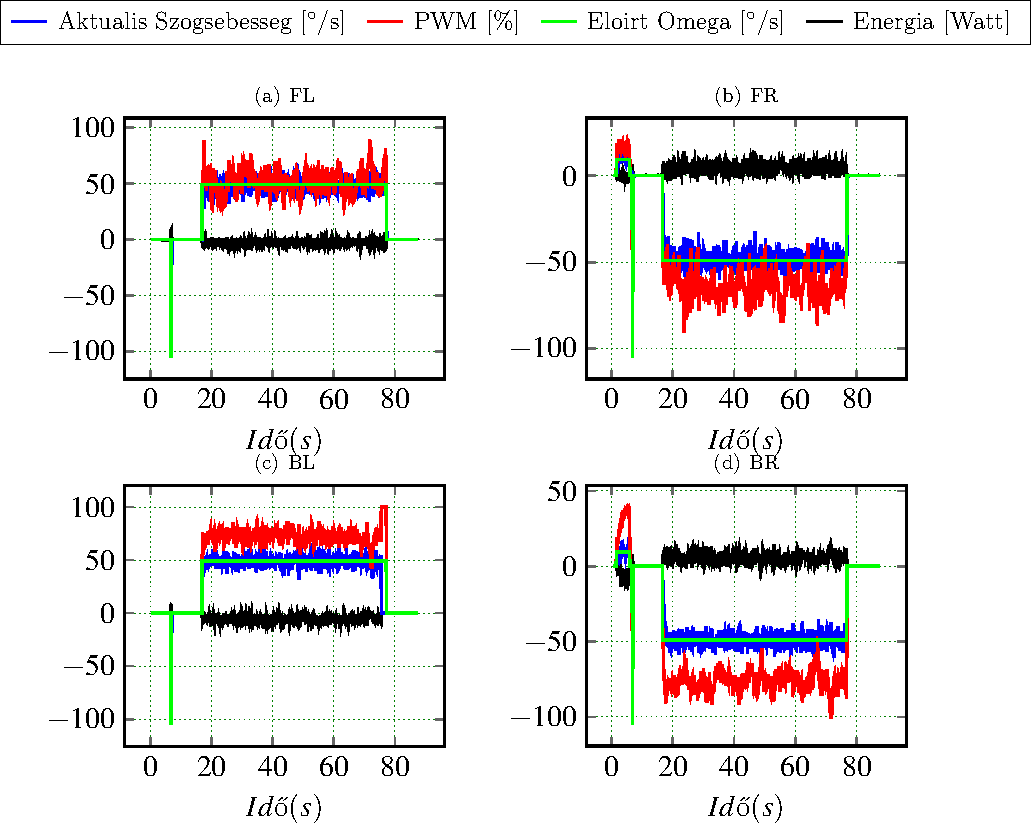
\includegraphics{tikz/Left_n50Right50x.pdf}
  \caption{$SSMR-4W$ típusú robot mozgása, tengelyekre bontva, kereksebessegek BL=FL=0 es a FR=BR= 50\degree/s}
  \label{fig:Left_n50Right50x}
\end{figure}


\begin{figure}[H]
  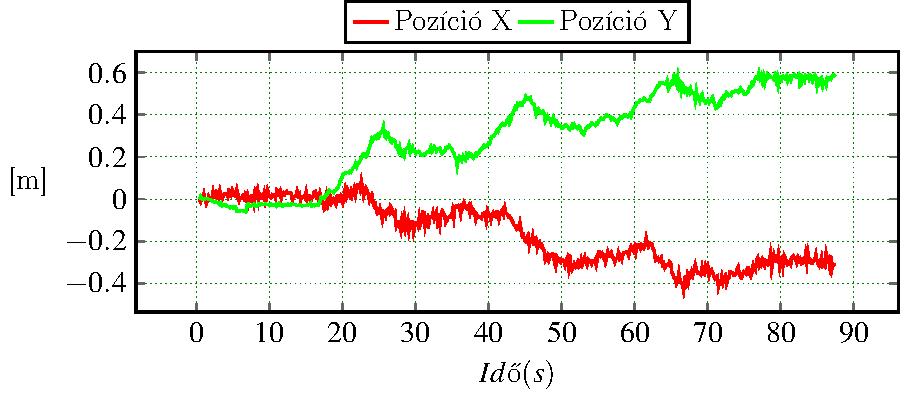
\includegraphics{tikz/Left_n50Right50a.pdf}
  \caption{$SSMR-4W$ típusú robot mozgása, tengelyekre bontva, kereksebessegek BL=FL=-50 es a FR=BR= 50\degree/s}
  \label{fig:Left_n50Right50a}
\end{figure}


\begin{figure}[H]
  \label{fig:Left_n50Right50b}
  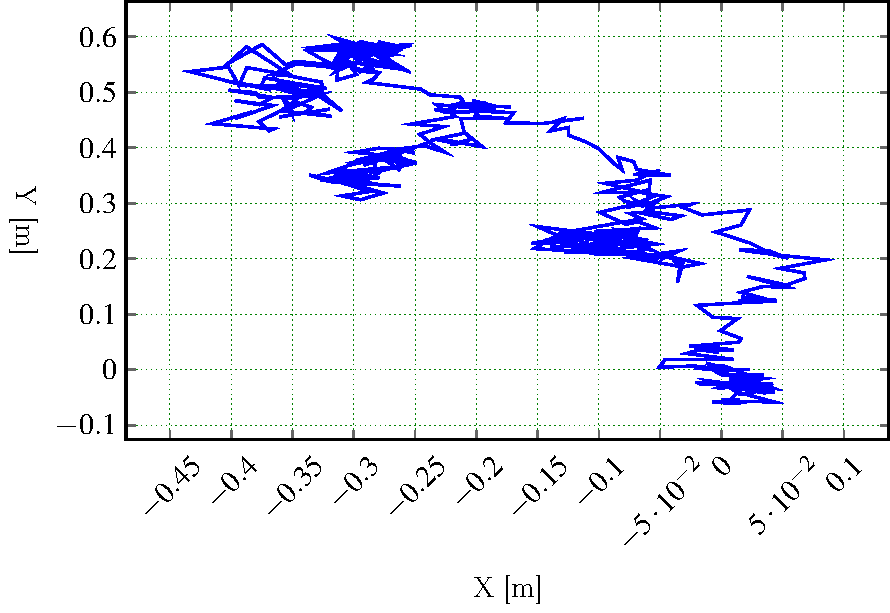
\includegraphics{tikz/Left_n50Right50b.pdf}
  \caption{$SSMR-4W$ típusú robot altal leirt palya, kereksebessegek BL=FL=-50 es a FR=BR= 50\degree/s}
\end{figure}



\begin{figure}[H]
  \label{fig:Left_n50Right50c}
  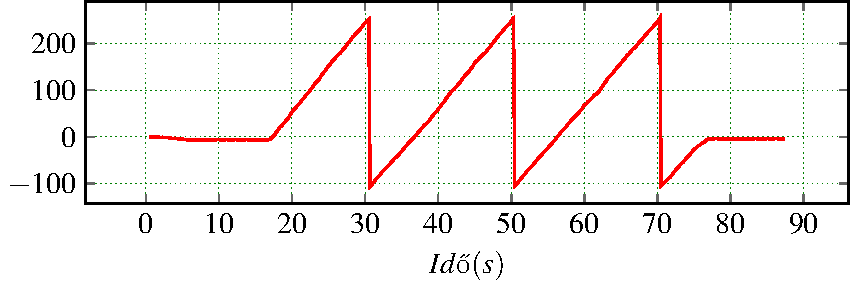
\includegraphics{tikz/Left_n50Right50c.pdf}
  \caption{$SSMR-4W$ típusú robot orientacioja, kereksebessegek BL=FL=-50 es a FR=BR= 50\degree/s}
\end{figure}


\begin{figure}[H]
  \label{fig:Left_n50Right50d}
  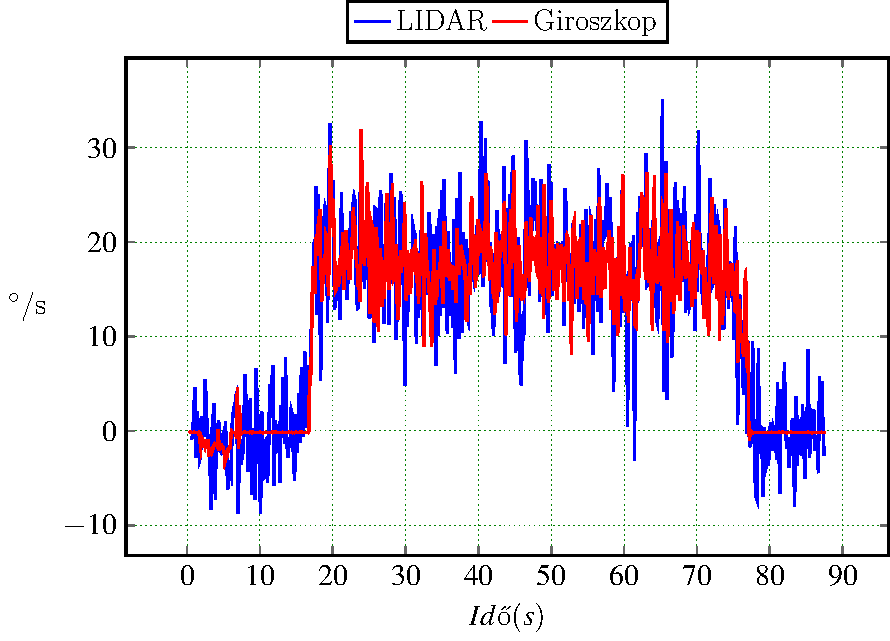
\includegraphics{tikz/Left_n50Right50d.pdf}
  \caption{$SSMR-4W$ típusú robot fordulasi szogsebessege, kereksebessegek BL=FL=-50 es a FR=BR= 50\degree/s}
\end{figure}











\subsection{Kavicsos talajon korpalyan mozgas}


\subsection{Kavicsos talajon korpalyan 50/15}
A \ref{fig:KorP0705a} megfigyelhető amint a robot kavicsos talajon differenciálisan fordul 80 másodpercen keresztül, ezalatt másfélszer körbefordul.

\renewcommand{\GlobalPath}{Meresek/Mozgasok/NormalMukodes/Korpalya_07_05_Kavicsos/}
\renewcommand{\secondImage}{*}

%kep a talajrol
%\input{Meresek/Mozgasok/KepekAFelszinrol.tex}

%1
%\input{Meresek/Mozgasok/FirstV1.tex}

\begin{figure}[H]
  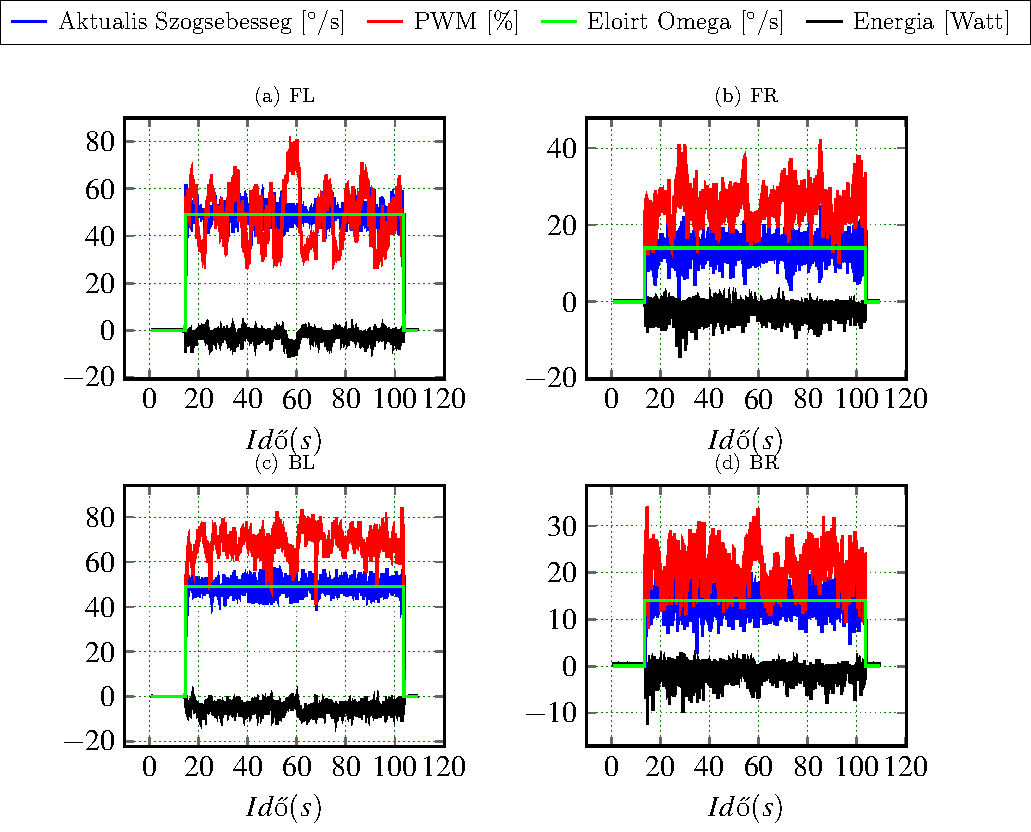
\includegraphics{tikz/KorP0705x.pdf}
  \caption{$SSMR-4W$ típusú robot mozgása, tengelyekre bontva, keréksebességek BL=FL=50\degree/s és a FR=BR=15\degree/s}
  \label{fig:KorP0705x}  
\end{figure}


\begin{figure}[H]
  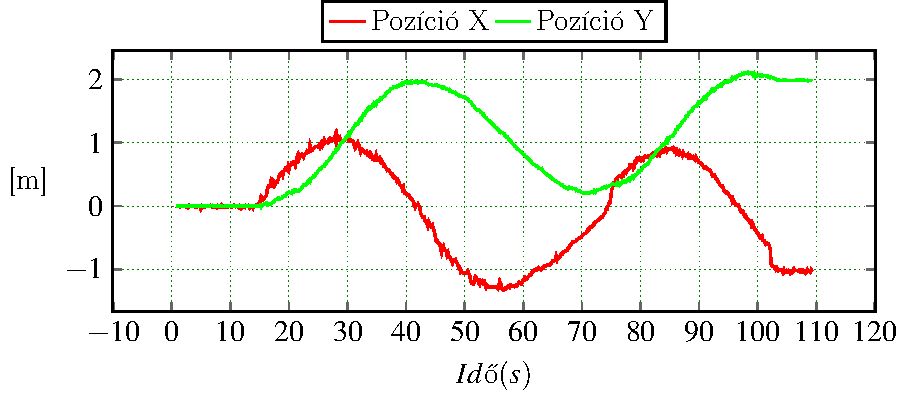
\includegraphics{tikz/KorP0705a.pdf}
  \caption{$SSMR-4W$ típusú robot mozgása, tengelyekre bontva, kerekszögsebességek BL=FL=50\degree/s és a FR=BR=15\degree/s}
  \label{fig:KorP0705a}  
\end{figure}


\begin{figure}[H]
  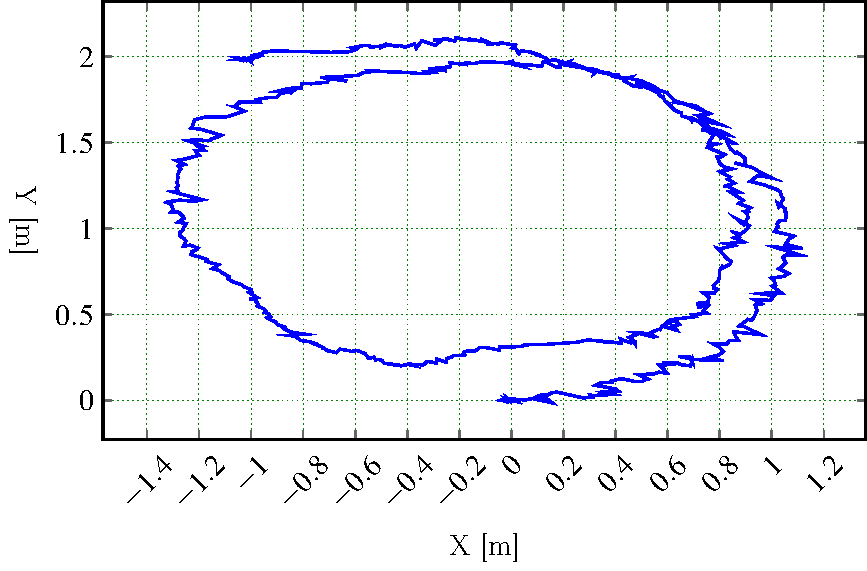
\includegraphics{tikz/KorP0705b.pdf}
  \caption{$SSMR-4W$ típusú robot altal leirt palya, kerekszögsebességek BL=FL=50\degree/s és a FR=BR=15\degree/s}
  \label{fig:KorP0705b}
\end{figure}

A körpalyán mozgás során a robot eltér a szabályos körtöl, és  látható a \ref{fig:KorP0705b} ábrán. A mérések nyilthurokan törének, nincs szabályzókör a pozicióra és a sebességkre.
A szögsebességet tekintve a robot 7\degree/s szögsebességet generál.


%\begin{figure}[H]
%  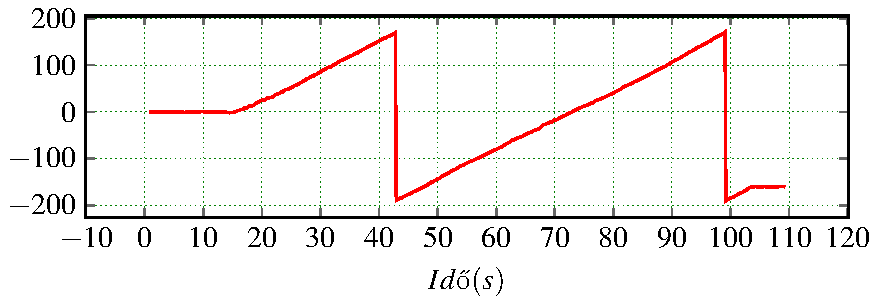
\includegraphics{tikz/KorP0705c.pdf}
%  \caption{$SSMR-4W$ típusú robot orientacioja, kerekszögsebességek %BL=FL=50\degree/s és a FR=BR=15\degree/s}
%  \label{fig:KorP0705c}
%\end{figure}


\begin{figure}[H]
\begin{center}
  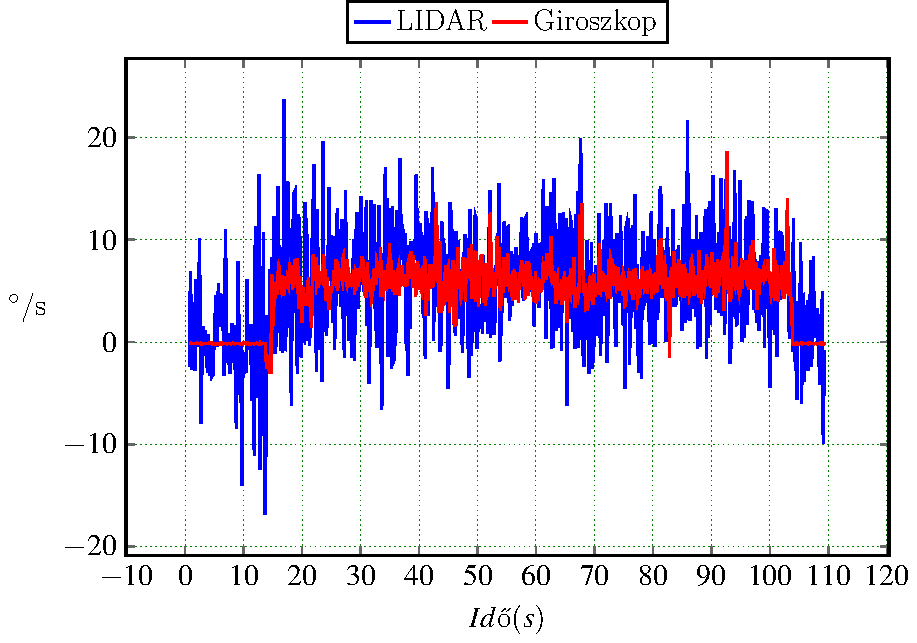
\includegraphics[scale=0.8]{tikz/KorP0705d.pdf}
\end{center}
  \caption{$SSMR-4W$ típusú robot fordulasi szögsebessége, kerekszögsebességek BL=FL=50\degree/s és a FR=BR=15\degree/s}
  \label{fig:KorP0705d}
\end{figure}


\begin{figure}[H]
\begin{center}
  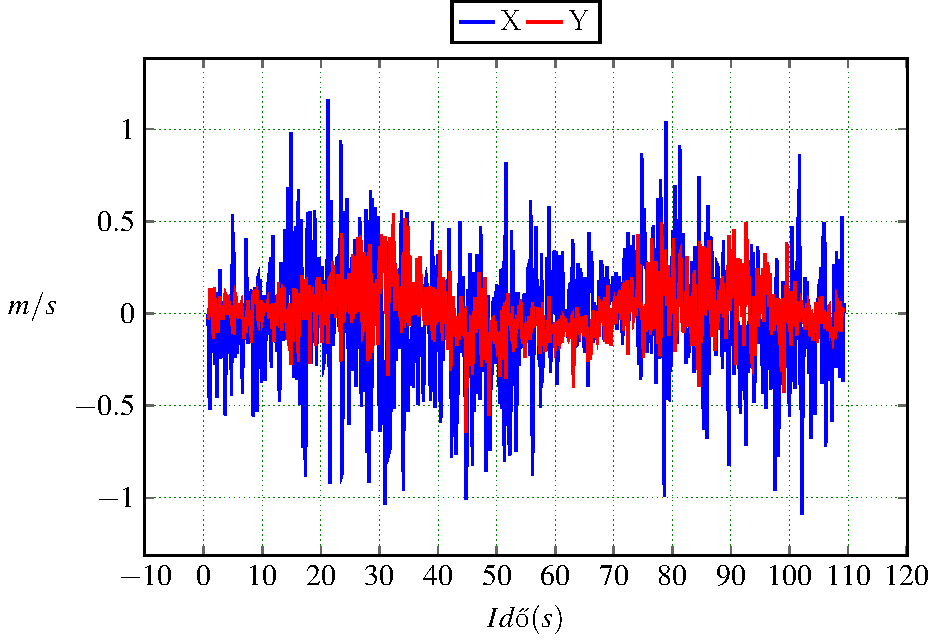
\includegraphics[scale=0.8]{tikz/KorP0705e.pdf}
\end{center}
  \caption{$SSMR-4W$ típusú robot egyenesvonalú sebességei, kerekszögsebességek BL=FL=50\degree/s és a FR=BR=15\degree/s}
  \label{fig:KorP0705e}
\end{figure}

A robot sebességét tekintve a \ref{fig:KorP0705e} látható hogy szinuszosan változuk a pozicióhoz hasonlóan,a robot kiss sebességü mozgása miatt a mérés zajos.
;
\subsection{Kavicsos talajon körpályán 50/25}

Az alábbi méréseknél 80-90s között a robot jobboldali kerekeit vezérlő H-híd túlmelegedése miatt a beléjük épített védelmi funkciónak köszönhetően leálltak így a jobboldali kerek leblokkoltak, így a mozgás pályája is megváltozott.


\renewcommand{\GlobalPath}{Meresek/Mozgasok/NormalMukodes/Korpalya_07_03_Kavicsos/}
\renewcommand{\secondImage}{*}

%kep a talajrol
%\input{Meresek/Mozgasok/KepekAFelszinrol.tex}

%1
%\input{Meresek/Mozgasok/FirstV1.tex}



\begin{figure}[H]
  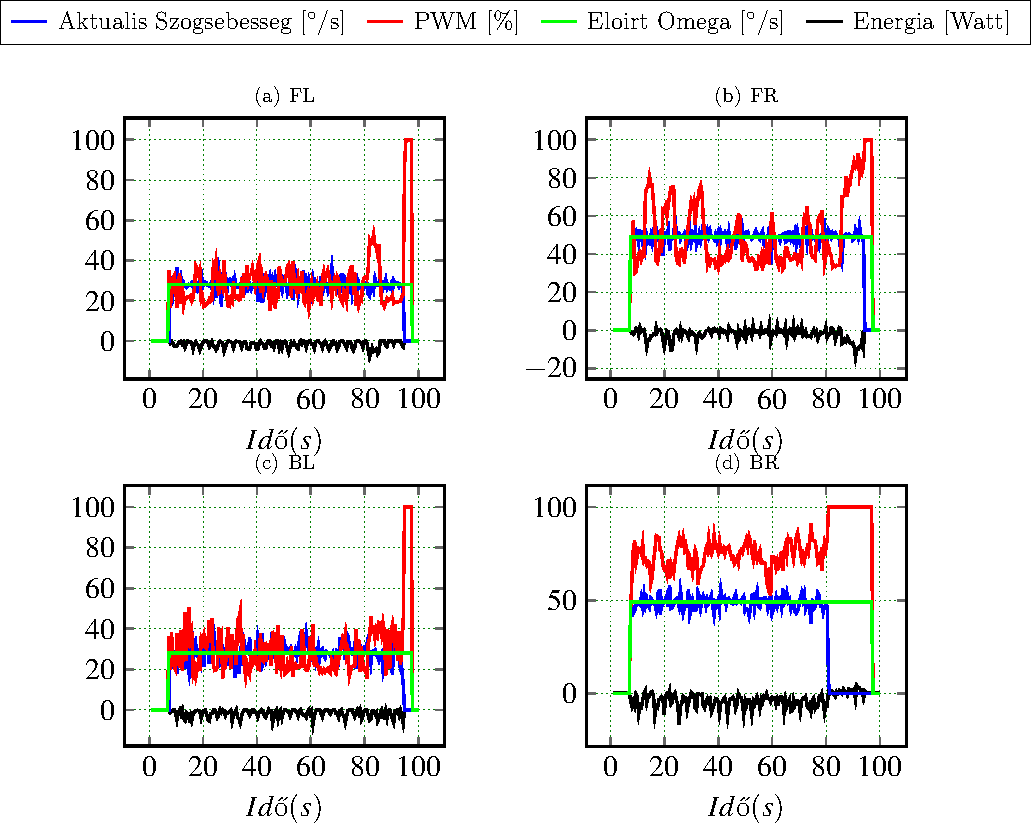
\includegraphics{tikz/KorP0703x.pdf}
  \caption{$SSMR-4W$ típusú robot motorvezérlő jelei, ha kerékszögsebességek BL=FL=25\degree/s és a FR=BR=50\degree/s}
  \label{fig:KorP0703x}
\end{figure}


\begin{figure}[H]
  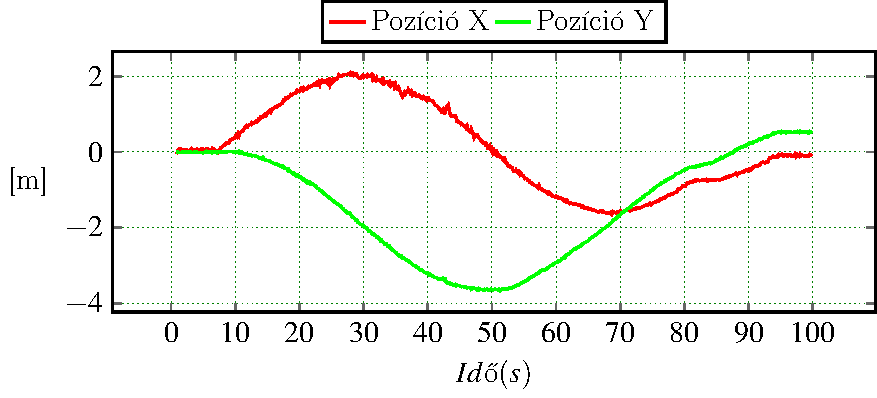
\includegraphics{tikz/KorP0703a.pdf}
  \caption{$SSMR-4W$ típusú robot mozgása, tengelyekre bontva, ha kerékszögsebességek BL=FL=25\degree/s és a FR=BR=50\degree/s }
  \label{fig:KorP0703a}
\end{figure}



\begin{figure}[H]
  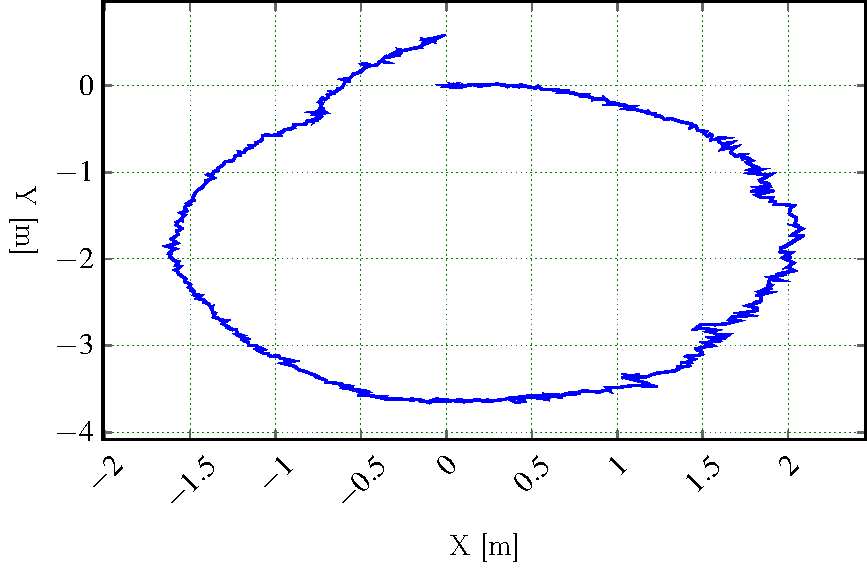
\includegraphics{tikz/KorP0703b.pdf}
  \caption{$SSMR-4W$ típusú robot által leírt pálya, ha kerékszögsebességek BL=FL=25\degree/s és a FR=BR=50\degree/s}
  \label{fig:KorP0703b}
\end{figure}


%\begin{figure}[H]
%  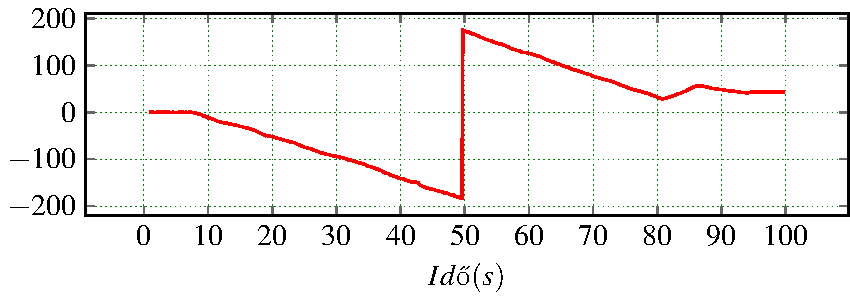
\includegraphics{tikz/KorP0703c.pdf}
%  \caption{$SSMR-4W$ típusú robot orientációja, ha kerékszögsebességek %BL=FL=25\degree/s és a FR=BR=50\degree/s}
%  \label{fig:KorP0703c}
%\end{figure}


\begin{figure}[H]
  \begin{center}
  	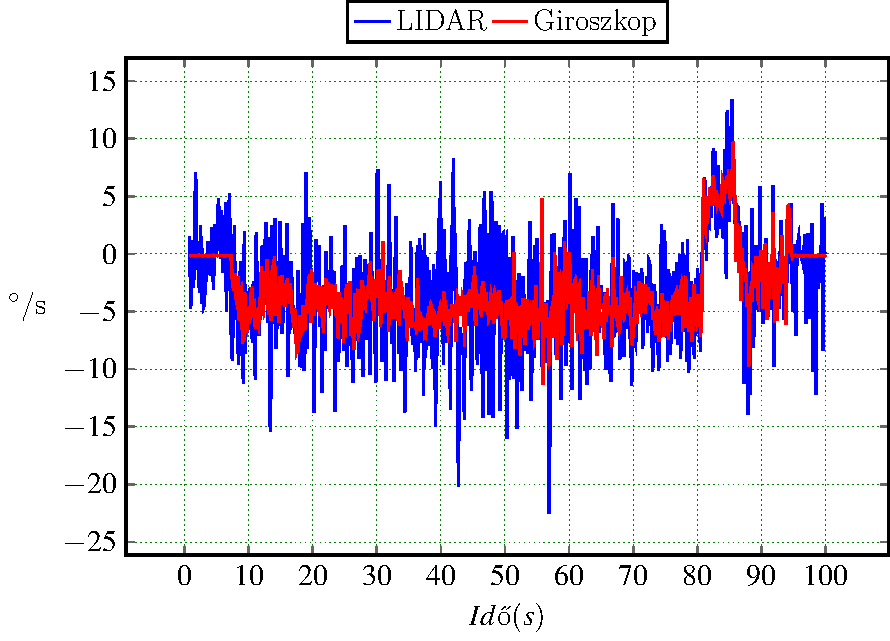
\includegraphics[scale=1]{tikz/KorP0703d.pdf}
  \end{center}
  \caption{$SSMR-4W$ típusú robot fordulási szögsebessége, ha kerékszögsebességek BL=FL=25\degree/s és a FR=BR=50\degree/s}
  \label{fig:KorP0703d}
\end{figure}

%\begin{figure}[H]
%  \includegraphics{tikz/KorP0703e.pdf}
%  \caption{$SSMR-4W$ típusú robot egyenesvonalu sebessegei, ha %kerékszögsebességek BL=FL=25\degree/s és a FR=BR=50\degree/s}
%  \label{fig:KorP0703e}
%\end{figure}


;

------------------------------------


\begin{figure}[H]
  \includegraphics{tikz/KorpalyakKavicsos.pdf}
  \caption{Kulombozo korpalyak}
  \label{fig:KorpalyakKavicsos}  
\end{figure}





\renewcommand{\GlobalPath}{Meresek/Mozgasok/GyergyoFuvesUdvar/M1/}
\renewcommand{\plotRotSpeed}{o}
\renewcommand{\plotSpeed}{o}
%
\subsubsection{Talajon valo mozgas meresi eredmenyei}


\renewcommand{\AbraFelirat}{$SSMR-4W$ tipusu robot kereknyomoerok kerekenkeni változása a sulypont fuggvenyebenddd}

%kep a talajrol


\renewcommand{\sources}{}
\renewcommand{\captionn}{Kep a felszinrol}
\renewcommand{\figlabel}{figm}


\begin{kep}
    \begin{figure}[H]%
    \begin{center}
    
    \subfloat[label a]{
        {\includegraphics[width=9cm]{\mand{\GlobalPath}{talaj1.jpg}} }
        \label{fig:ex3-a}
    }%
    
    \ifthenelse{\equal{\secondImage}{*}}
    {}
    {
        \qquad
        \subfloat[label b]{{\includegraphics[width=9cm]{\mand{\GlobalPath}{talaj1.jpg}} }}%
    }
  
    \label{fig:example}%
    \end{center}
\end{figure}
\end{kep}

\renewcommand{\secondImage}{*}



%1
 %1
    \begin{figure}
    
        %-------------------------------------------------Joint Adatok---------------
        \begin{subfigure}{\textwidth}
            \begin{center}
        
            \input{\mand{\GlobalPath}{L.tex}}
            \pgfplotstableread{NodeLeft.dat}{\leftNode}

            
            \input{\mand{\GlobalPath}{R.tex}}
            \pgfplotstableread{NodeRight.dat}{\rightNode}

        
            \begin{tikzpicture}
            \pgfplotsset{every axis plot/.append style={very thick}}
            \setcaptionsubtype
            
            % megjelenites beallitasai
            
            \begin{groupplot}[%
                        ,group style={%
                            ,group name=my plots
                            ,group size=2 by 2
                            ,vertical sep=1.8cm,
                            ,horizontal sep = 2.4cm,
                            ,ylabels at=edge left
                        }
                        ,width=7cm
                        ,height=6cm
                        ,try min ticks=5
                        ,xlabel={\bfseries{\emph{\idoFelirat}}}
                        ,zlabel={\bfseries{\emph{kg}}}
                        %%ha kell y felirat az elso ketore
                        %,ylabel={\bfseries{\degree$/s$}}
                        %,ylabel style={rotate=-90}
                        %,xtick={0,10,...,60},
                        %,minor tick num=5
                        %,xtick distance=10
                        %,ytick distance=25
                        ,grid=major%both
                        ,every both grid/.style={gray, opacity=0.7},
                        view={0}{90},
                        legend columns=2,
                        %xmin=0,xmax=0.65,
                        %ymin=0,ymax=0.65,
                       % zmin=-5,zmax=60,
                        ]
            %% ide jonnek a adatok. 
            
            %ha kell felirat be kell teni a nextplot[] parameterei koze
            % \nextgroupplot[ylabel=\degree$/s$, ylabel style={rotate=-90},legend to name={CommonLegend},legend style={legend columns=2}]
            \nextgroupplot[]
                \addplot [color=green,each nth point={\nth}] table [header=true, x=Time, y=refOmegaA] {\leftNode};\label{plots:plot3}
                \addplot [color=black,each nth point={\nth}] table [header=true, x=Time, y=effortA] {\leftNode};\label{plots:plot4}
                \addplot [color=blue,each nth point={\nth}] table [header=true, x=Time, y=omegaA] {\leftNode}; \label{plots:plot1}
                \addplot [color=red,each nth point={\nth}] table [header=true, x=Time, y=pwmA] {\leftNode};\label{plots:plot2}
                \coordinate (top) at (rel axis cs:0,1);% coordinate at top of the first plot
            
            \nextgroupplot[]
                \addplot [color=green,each nth point={\nth}] table [header=true, x=Time, y=refOmegaA] {\rightNode};
                \addplot [color=black,each nth point={\nth}] table [header=true, x=Time, y=effortA] {\rightNode};
                \addplot [color=blue,each nth point={\nth}] table [header=true, x=Time, y=omegaA] {\rightNode};
                \addplot [color=red,each nth point={\nth}] table [header=true, x=Time, y=pwmA] {\rightNode};
                    
            \nextgroupplot[]
                \addplot [color=green,each nth point={\nth}] table [header=true, x=Time, y=refOmegaB] {\leftNode};
                \addplot [color=black,each nth point={\nth}] table [header=true, x=Time, y=effortB] {\leftNode};
                \addplot [color=blue,each nth point={\nth}] table [header=true, x=Time, y=omegaB] {\leftNode};
                \addplot [color=red,each nth point={\nth}] table [header=true, x=Time, y=pwmB] {\leftNode};
                   
            \nextgroupplot[]
                \addplot [color=green,each nth point={\nth}] table [header=true, x=Time, y=refOmegaB] {\rightNode};
                \addplot [color=black,each nth point={\nth}] table [header=true, x=Time, y=effortB] {\rightNode};
                \addplot [color=blue,each nth point={\nth}] table [header=true, x=Time, y=omegaB] {\rightNode};
                \addplot [color=red,each nth point={\nth}] table [header=true, x=Time, y=pwmB] {\rightNode};
                \coordinate (bot) at (rel axis cs:1,0);% coordinate at bottom of the last plot
            \end{groupplot}
            
            %\path [nodes={anchor=south,rotate=90,font=\large\bfseries,midway}]
            %  (my plots c1r1.outer north west)--(my plots c1r2.outer south west)
            %    node {Testing of Parameters 1}
            %  (my plots c2r1.outer north west)--(my plots c2r2.outer south west)
            %    node {Testing of Parameters 2};
            
            % legend
            \node[text width=.5\linewidth,align=center,anchor=south] at (my plots c1r1.north) {\caption[]{FL\label{subplot:one}}};
            \node[text width=.5\linewidth,align=center,anchor=south] at (my plots c2r1.north) {\caption[]{FR\label{subplot:two}}};
            \node[text width=.5\linewidth,align=center,anchor=south] at (my plots c1r2.north) {\caption[]{BL\label{subplot:three}}};
            \node[text width=.5\linewidth,align=center,anchor=south] at (my plots c2r2.north) {\caption[]{BR\label{subplot:four}}};
            
            %\path (top-|current bounding box.west)-- 
            %      node[anchor=south,rotate=90] {throughput} 
            %      (bot-|current bounding box.west);
            % legend
            \path (top|-current bounding box.north)--
                  coordinate(legendpos)
                  (bot|-current bounding box.north);
            \matrix[
                matrix of nodes,
                anchor=south,
                draw,
                inner sep=0.2em,
                draw
              ]at([yshift=1ex]legendpos)
              {
                \ref{plots:plot1}& Aktualis Szogsebesseg [\degree$/s$]&[5pt]
                \ref{plots:plot2}& PWM [$\%$] &[5pt]
                \ref{plots:plot3}& Eloirt Omega [\degree$/s]$
                \ref{plots:plot4}& Energia $[Watt]$ &[5pt]\\
            };
           % \centering
            \end{tikzpicture}
            \end{center}
        \end{subfigure}
        
        \iffalse
        %-------------------------------------------------Power Adatok---------------
        \newline
        \begin{subfigure}{\textwidth}
        \begin{center}
        \input{\mand{\GlobalPath}{Power.tex}}
        \pgfplotstableread{Power.dat}{\power}
        
        
        \begin{tikzpicture}
        \pgfplotsset{every axis plot/.append style={very thick}}
        \setcaptionsubtype
        
        % megjelenites beallitasai
        
        \begin{groupplot}[%
                    ,group style={%
                        ,group name=my plots
                        ,group size=1 by 1
                        ,vertical sep=2cm,
                        ,horizontal sep = 0cm,
                        ,ylabels at=edge left
                    }
                    ,width=14.5cm
                    ,height=6cm
                    ,try min ticks=5
                    ,xlabel={\bfseries{\emph{\idoFelirat}}}
                    %,ylabel={\bfseries{\emph{A}}}
                    %,zlabel={\bfseries{\emph{kg}}}
                    ,grid=both
                    ,every both grid/.style={gray, opacity=0.5}
                    ,view={0}{90},
                    %,xtick distance=10
                    %,minor tick num=5
                    %,ytick distance=5
                    %xmin=0,xmax=0.65,
                    %ymin=0,ymax=0.65,
                    %zmin=-5,zmax=60,
                    ]
        %% ide jonnek a adatok.            
                    
        \nextgroupplot[ylabel=\emph{}, ylabel style={rotate=-90}]
         \addplot [color=red,each nth point={\nth}] table [header=true, x=Time, y=voltage] {\power};\label{plots:plot11}
         \addplot [color=green,each nth point={\nth}] table [header=true, x=Time, y=current]{\power};\label{plots:plot12}
         \addplot [color=black,each nth point={\nth}] table [header=true, x=Time, y=power] {\power};\label{plots:plot13}
        \end{groupplot}
        
        %\path [nodes={anchor=south,rotate=90,font=\large\bfseries,midway}]
        %  (my plots c1r1.outer north west)--(my plots c1r2.outer south west)
        %    node {Testing of Parameters 1}
        %  (my plots c2r1.outer north west)--(my plots c2r2.outer south west)
        %    node {Testing of Parameters 2};
        
        % legend
        \node[text width=.5\linewidth,align=center,anchor=south] at (my plots c1r1.north) {\caption[]{Energia Fogyasztas\label{subplot:one}}};
        
        %\path (top-|current bounding box.west)-- 
            %      node[anchor=south,rotate=90] {throughput} 
            %      (bot-|current bounding box.west);
            % legend
            \path (top|-current bounding box.north)--
                  coordinate(legendpos)
                  (bot|-current bounding box.north);
            \matrix[
                matrix of nodes,
                anchor=south,
                draw,
                inner sep=0.2em,
                draw
              ]at([yshift=1ex]legendpos)
              {
                \ref{plots:plot11}&  Akumlator Feszultsege [V]&[5pt]
                \ref{plots:plot12}& Akkumlator Arama [A] &[5pt]
                \ref{plots:plot13}& Teljesitmeny [W] \\
            };
        
        %\centering
        \end{tikzpicture}
        \end{center}
        \end{subfigure}
        % Caption
        %\caption[]{$SSMR-4W$ tipusu robot kereknyomoerok kerekenkeni változása a sulypont fuggvenyeben}\label{abserror}
        \fi
    \end{figure}

%2
    %2
    \begin{figure}[H]
        %\ContinuedFloat
        %-------------------------------------------------Pozicio X es Y Adatok---------------
       % \newline
        \begin{subfigure}{\textwidth}
        \begin{center}
           \input{\mand{\GlobalPath}{Pos.tex}}
            \pgfplotstableread{PositionOrientation.dat}{\pos}
            \centering
            \begin{tikzpicture}
            \pgfplotsset{every axis plot/.append style={very thick}}
            \setcaptionsubtype
            
            % megjelenites beallitasai
            
            \begin{groupplot}[%
                        ,group style={%
                            ,group name=my plots
                            ,group size=1 by 1
                            ,vertical sep=2cm,
                            ,horizontal sep = 0cm,
                            ,ylabels at=edge left
                        }
                        ,width=14.5cm
                        ,height=6cm
                        ,try min ticks=5
                        ,xlabel={\bfseries{\emph{\idoFelirat}}}
                        %,ylabel={\bfseries{\emph{A}}}
                        %,zlabel={\bfseries{\emph{kg}}}
                        ,grid=both
                        ,every both grid/.style={gray, opacity=0.5}
                        ,view={0}{90},
                        %,xtick distance=10
                        %,ytick distance=0.4
                        %,minor tick num=5
                        %xmin=0,xmax=0.65,
                        %ymin=0,ymax=0.65,
                        %zmin=-5,zmax=60,
                        ]
            %% ide jonnek a adatok.            
                        
            \nextgroupplot[ylabel=\emph{m}, ylabel style={rotate=-90}]
             \addplot [color=red,each nth point={\nth}] table [header=true, x=Time, y=poseX] {\pos};\label{plots:plot21}
             %\addlegendentry{Pozíció X [m]} 
             \addplot [color=green,each nth point={\nth}] table [header=true, x=Time, y=poseY]{\pos};\label{plots:plot22}                            %\addlegendentry{Pozíció Y [m]} 
            \end{groupplot}
            
            %\path [nodes={anchor=south,rotate=90,font=\large\bfseries,midway}]
            %  (my plots c1r1.outer north west)--(my plots c1r2.outer south west)
            %    node {Testing of Parameters 1}
            %  (my plots c2r1.outer north west)--(my plots c2r2.outer south west)
            %    node {Testing of Parameters 2};
            
            % legend
            \node[text width=.5\linewidth,align=center,anchor=south] at (my plots c1r1.north) {\caption[]{Robot Pozíció Tengelyekre           \label{subplot:\figlabela}}};
            
            %\path (top-|current bounding box.west)-- 
                %      node[anchor=south,rotate=90] {throughput} 
                %      (bot-|current bounding box.west);
                % legend
                \path (top|-current bounding box.north)--
                      coordinate(legendpos)
                      (bot|-current bounding box.north);
                \matrix[
                    matrix of nodes,
                    anchor=south,
                    draw,
                    inner sep=0.2em,
                    draw
                  ]at([yshift=1ex]legendpos)
                  {
                    \ref{plots:plot21}&Pozíció X [m] &[5pt]
                    \ref{plots:plot22}&Pozíció Y [m] &[5pt]\\
                };
            
            %\centering
            \end{tikzpicture}
            \end{center}
        \end{subfigure}
        
        %-------------------------------------------------Palya Adatok---------------
      %  \newline
        \begin{subfigure}{\textwidth}
           \begin{center}
            \input{\mand{\GlobalPath}{/Pos.tex}}
            \pgfplotstableread{PositionOrientation.dat}{\position}
            
            \begin{tikzpicture}
                \pgfplotsset{every axis plot/.append style={very thick}}
                \setcaptionsubtype
            
                % megjelenites beallitasai
            
                \begin{groupplot}[%
                        ,group style={%
                            ,group name=my plots
                            ,group size=1 by 1
                            ,vertical sep=2cm,
                            ,horizontal sep = 0cm,
                            ,ylabels at=edge left
                        }
                        ,width=14.5cm
                        ,height=9cm
                        %,try min ticks=5
                        ,xlabel={\bfseries{\emph{m}}}
                        ,ylabel={\bfseries{\emph{m}}}
                        ,zlabel={\bfseries{\emph{\idoFelirat}}}
                        ,grid=both
                        ,every both grid/.style={gray, opacity=0.5}
                        ,view={45}{45}
                        %,xtick distance=0.25
                        %,ytick distance=0.25
                        %,minor tick num=5
                        ,xticklabel style={rotate=45},
                        ,ylabel style={rotate=-90}
                        %xmin=0,xmax=0.65,
                        %ymin=0,ymax=0.65,
                       % zmin=-5,zmax=60,
                        ]
                    %% ide jonnek a adatok.            
                                
                    %\nextgroupplot[ylabel=\emph{A}, ylabel style={rotate=-90}]
                    \nextgroupplot[]
                           % \addplot3 []  table [header=true, x=poseX, y=poseY, z=Time] {\position};
                           
                            \addplot [color=blue,each nth point={\nth}] table [header=true, x=poseX, y=poseY] {\position};
                            
                            %\addplot [color=blue] table [header=true, x=poseX, y=poseY] {\position};
                         %%   \addplot[red,quiver={u=u,v=v}] table [header=true, x=poseX, y=poseY, u=poseX, v=poseY] {\position};
        
        
        
        
            \end{groupplot}
            
                %\path [nodes={anchor=south,rotate=90,font=\large\bfseries,midway}]
                %  (my plots c1r1.outer north west)--(my plots c1r2.outer south west)
                %    node {Testing of Parameters 1}
                %  (my plots c2r1.outer north west)--(my plots c2r2.outer south west)
                %    node {Testing of Parameters 2};
                
                % legend
                \node[text width=.5\linewidth,align=center,anchor=south] at (my plots c1r1.north) {\caption[]{Robot Által Leirt Pálya     \label{subplot:\figlabelb}}};
                
                %\centering
            \end{tikzpicture}
            \end{center}
    \end{subfigure}
        
        %-------------------------------------------------Orientacio Adatok---------------
       % \newline
        \begin{subfigure}{\textwidth}
        \begin{center}
        \input{\mand{\GlobalPath}{Pos.tex}}
        \pgfplotstableread{PositionOrientation.dat}{\pos}
        
        \begin{tikzpicture}
        \pgfplotsset{every axis plot/.append style={very thick}}
        \setcaptionsubtype
        
        % megjelenites beallitasai
        
        \begin{groupplot}[%
                    ,group style={%
                        ,group name=my plots
                        ,group size=1 by 1
                        ,vertical sep=2cm,
                        ,horizontal sep = 0cm,
                        ,ylabels at=edge left
                    }
                    ,width=14.5cm
                    ,height=5cm
                    ,try min ticks=5
                    ,xlabel={\bfseries{\emph{\idoFelirat}}}
                    %,ylabel={\bfseries{\emph{A}}}
                    %,zlabel={\bfseries{\emph{kg}}}
                    ,grid=both
                    ,every both grid/.style={gray, opacity=0.5}
                    ,view={0}{90},
                    %,xtick distance=10
                    %,ytick distance=20
                    %,minor tick num=5
                    %xmin=0,xmax=0.65,
                    %ymin=0,ymax=0.65,
                    %zmin=-5,zmax=60,
                    ]
        %% ide jonnek a adatok.            
                    
        \nextgroupplot[ylabel=\emph{$[\degree]$}], ylabel style={rotate=-90}]
        \addplot [color=red,each nth point={\nth}] table [header=true, x=Time, y=orZ] {\pos};\label{plots:plot41}
        \end{groupplot}
        
        %\path [nodes={anchor=south,rotate=90,font=\large\bfseries,midway}]
        %  (my plots c1r1.outer north west)--(my plots c1r2.outer south west)
        %    node {Testing of Parameters 1}
        %  (my plots c2r1.outer north west)--(my plots c2r2.outer south west)
        %    node {Testing of Parameters 2};
        
        % legend
        \node[text width=.5\linewidth,align=center,anchor=south] at (my plots c1r1.north) {\caption[]{Orientáció \label{subplot:\figlabelc}}};
        
        
       % \centering
        \end{tikzpicture}
        \end{center}
        \end{subfigure}
    
        
        % Caption
        \ifthenelse{\equal{\captionn}{*}}
        {}
        {\captionof{figure}{\captionn}}
        \renewcommand{\captionn}{*}
        \label{subplot:\figlabel}
       
    \end{figure}
    
        \renewcommand{\figlabel}{*}
        \renewcommand{\figlabela}{*}
        \renewcommand{\figlabelb}{*}
        \renewcommand{\figlabelc}{*}

%3
%    %3
    \begin{figure}
        %\ContinuedFloat
        \input{\mand{\GlobalPath}{Pos.tex}}
        \ifthenelse{\equal{\plotSpeed}{*}}
        { }
        {
        \newline
        \begin{subfigure}{\textwidth}
            \begin{center}

            \pgfplotstableread{PositionOrientation.dat}{\position}
            
            %-------------------------------------------------Sebesseg Adatok---------------
            \begin{tikzpicture}
                \pgfplotsset{every axis plot/.append style={very thick}}
                \setcaptionsubtype
            
                % megjelenites beallitasai
            
                \begin{groupplot}[%
                        ,group style={%
                            ,group name=my plots
                            ,group size=1 by 1
                            ,vertical sep=2cm,
                            ,horizontal sep = 0cm,
                            ,ylabels at=edge left
                        }
                        ,width=14.5cm
                        ,height=10cm
                        ,try min ticks=5
                        ,ylabel={\bfseries{\emph{$m/s$}}}
                        ,xlabel={\bfseries{\emph{\idoFelirat}}}
                        %,zlabel={\bfseries{\emph{m}}}
                        ,grid=both
                        ,every both grid/.style={gray, opacity=0.5}
                        ,view={0}{90}
                        %,xtick distance=10
                        %,ytick distance=0.1
                        ,ylabel style={rotate=-90}
                        %xmin=0,xmax=0.65,
                        %ymin=0,ymax=0.65,
                       % zmin=-5,zmax=60,
                        ]
                    %% ide jonnek a adatok.            
                                
                    %\nextgroupplot[ylabel=\emph{A}, ylabel style={rotate=-90}]
                    \nextgroupplot[]
                            \addplot [color=blue,each nth point={\nth}] table [header=true, x=Time, y=speedX] {\position}; \label{plots:plot51}
                            \addplot [color=red,each nth point={\nth}] table [header=true, x=Time, y=speedY] {\position}; \label{plots:plot52}
                         %%   \addplot[red,quiver={u=u,v=v}] table [header=true, x=poseX, y=poseY, u=poseX, v=poseY] {\position};
        
        
        
        
            \end{groupplot}
            
                %\path [nodes={anchor=south,rotate=90,font=\large\bfseries,midway}]
                %  (my plots c1r1.outer north west)--(my plots c1r2.outer south west)
                %    node {Testing of Parameters 1}
                %  (my plots c2r1.outer north west)--(my plots c2r2.outer south west)
                %    node {Testing of Parameters 2};
                
                % legend
                \node[text width=.5\linewidth,align=center,anchor=south] at (my plots c1r1.north) {\caption[]{Robot Sebessége a Globális Koordináta Rendszerben
               \label{subplot:\figlabela}}};
                
                      %\path (top-|current bounding box.west)-- 
                %      node[anchor=south,rotate=90] {throughput} 
                %      (bot-|current bounding box.west);
                % legend
                \path (top|-current bounding box.north)--
                      coordinate(legendpos)
                      (bot|-current bounding box.north);
                \matrix[
                    matrix of nodes,
                    anchor=south,
                    draw,
                    inner sep=0.2em,
                    draw
                  ]at([yshift=1ex]legendpos)
                  {
                    \ref{plots:plot51}& Sebesség X &[5pt] 
                    \ref{plots:plot52}& Sebesség Y &[5pt]\\
                  };
                
                %\centering
            \end{tikzpicture}
            \end{center}
        \end{subfigure}
        }
        
        \ifthenelse{\equal{\plotRotSpeed}{*}}
        { }
        { 
        %-------------------------------------------------Fordulasi Sebesseg Adatok---------------
        \newline
        \input{\mand { \GlobalPath}{Pos.tex}}
        \pgfplotstableread{PositionOrientation.dat}{\position}
        
        \input{\mand{\GlobalPath}{ImuA.tex}}
        \pgfplotstableread{ImuA.dat}{\imua}
        
        \begin{subfigure}{\textwidth}
            \begin{center}

            
            \begin{tikzpicture}
                \pgfplotsset{every axis plot/.append style={very thick}}
                \setcaptionsubtype
            
                % megjelenites beallitasai
            
                \begin{groupplot}[%
                        ,group style={%
                            ,group name=my plots
                            ,group size=1 by 1
                            ,vertical sep=2cm,
                            ,horizontal sep = 0cm,
                            ,ylabels at=edge left
                        }
                        ,width=14.5cm
                        ,height=10cm
                        ,try min ticks=5
                        ,ylabel={\bfseries{\emph{\degree/s}}}
                        ,xlabel={\bfseries{\emph{\idoFelirat}}}
                        %,zlabel={\bfseries{\emph{m}}}
                        ,grid=both
                        ,every both grid/.style={gray, opacity=0.5}
                        ,view={0}{90}
                        %,xtick distance=10
                        %,ytick distance=10
                        ,ylabel style={rotate=-90}
                        %xmin=0,xmax=0.65,
                        %ymin=0,ymax=0.65,
                       % zmin=-5,zmax=60,
                        ]
                    %% ide jonnek a adatok.            
                                
                    %\nextgroupplot[ylabel=\emph{A}, ylabel style={rotate=-90}]
                    \nextgroupplot[]
                            \addplot [color=blue,each nth point={\nth}] table [header=true, x=Time, y=omegaZ] {\position}; \label{plots:plot61}
                            \addplot [color=red,each nth point={\nth}] table [header=true, x=Time, y expr=\thisrow{gZ}*-1] {\imua}; \label{plots:plot62}
                         %%   \addplot[red,quiver={u=u,v=v}] table [header=true, x=poseX, y=poseY, u=poseX, v=poseY] {\position};
        
        
        
        
            \end{groupplot}
            
                %\path [nodes={anchor=south,rotate=90,font=\large\bfseries,midway}]
                %  (my plots c1r1.outer north west)--(my plots c1r2.outer south west)
                %    node {Testing of Parameters 1}
                %  (my plots c2r1.outer north west)--(my plots c2r2.outer south west)
                %    node {Testing of Parameters 2};
                
                % legend
                \node[text width=.5\linewidth,align=center,anchor=south] at (my plots c1r1.north) {\caption[]{Robot Forgási Sebessége 
                \label{subplot:\figlabelb}}};
                
                        %\path (top-|current bounding box.west)-- 
                %      node[anchor=south,rotate=90] {throughput} 
                %      (bot-|current bounding box.west);
                % legend
                \path (top|-current bounding box.north)--
                      coordinate(legendpos)
                      (bot|-current bounding box.north);
                \matrix[
                    matrix of nodes,
                    anchor=south,
                    draw,
                    inner sep=0.2em,
                    draw
                  ]at([yshift=1ex]legendpos)
                  {
                    \ref{plots:plot61}& LIDAR  &[5pt] 
                    \ref{plots:plot62}& Giroszkop  &[5pt]\\
                };
                
               % \centering
            \end{tikzpicture}
            \end{center}
            
        \end{subfigure}
        }
        
        \renewcommand{\figlabela}{*}
        \renewcommand{\figlabelb}{*}
        
        % Caption
        \ifthenelse{\equal{\captionn}{*}}
        {}
        {\captionof{figure}{\captionn}}
        \renewcommand{\captionn}{*}

    
    \end{figure}

%Statistic
\DTLsetseparator{ = }% Set the separator between the columns. Could be
% anything you like. Whitespaces are not trimmed, so you have to set
%them as part of the separator.

\input{\mand{\GlobalPath}{Statistic.tex}}

        %\input{\mand{\GlobalPath}{Pos.tex}}
        %\pgfplotstableread{PositionOrientation.dat}{\pos}

\DTLdeletedb{mydataStat}
\DTLloaddb[noheader, keys={thekey,thevalue}]{mydataStat}{statistic.dat}
% Loads mydata.dat with column headers 'thekey' and 'thevalue'

\renewcommand{\missingcommand}[1]{\DTLfetch{mydataStat}{thekey}{#1}{thevalue}}

\begin{table}[H]
\begin{center}
    \begin{tabular}{llll}
        \hline
        Tulajdonság          & Node  & érték                                & Mértékegység                      \\ \hline
        Ossz sebesseg hiba   & FL & \missingcommand{SumErrorSpeedFL}        &   $[\degree/s]$                   \\
                             & BL & \missingcommand{SumErrorSpeedBL}        &   $[\degree/s]$                   \\
                             & FR & \missingcommand{SumErrorSpeedFR}        &   $[\degree/s]$                   \\
                             & BR & \missingcommand{SumErrorSpeedBR}        &   $[\degree/s]$                   \\
        Energia  fogyasztasa & FL & \missingcommand{PowerConsuptionFL}      &   $[W]$                           \\
                             & BL & \missingcommand{PowerConsuptionBL}      &   $[W]$                           \\
                             & FR & \missingcommand{PowerConsuptionFR}      &   $[W]$                           \\
                             & BR & \missingcommand{PowerConsuptionBR}      &   $[W]$                           \\
        Sulypont X           &    & \missingcommand{SulyPontX}              &   $[m]$                           \\
        Sulypont Y           &    & \missingcommand{SulyPontY}              &   $[m]$                           \\
        Ossz fordulas        &    & \missingcommand{Elfordulas}           &   $[\degree]$                     \\
        Megtett ut           &    & \missingcommand{Elmozdulas}              &   $[m]$                           \\
        Max Sebesseg         &    & \missingcommand{MaxSebesseg}            &   $[m\s]$                         \\
        Max ford Sebesseg    &    & \missingcommand{MaxFordulasiSebesseg}   &   $[\degree/s]$                   \\
    \end{tabular}
    \end{center}
\end{table}

%Imu
%   
    
    \begin{figure}[H]
        %\ContinuedFloat
        
            \tikzsetnextfilename{\figlabel}   
    
            \centering
             \input{\mand{\GlobalPath}{ImuA.tex}}
            \pgfplotstableread{ImuA.dat}{\imua}
            
            
             \begin{tikzpicture}
    
        \pgfplotsset{every axis plot/.append style={very thick}}
        \pgfplotsset{every axis legend/.append style={
        at={(0.5,1.03)},
        anchor=south}}
        
        \begin{axis}[
                ,width=14.5cm
                ,height=10cm
                ,try min ticks=5
                ,xlabel={\bfseries{\emph{\idoFelirat}}}
                ,ylabel={\bfseries{\emph{$m/{s^2}$}}}
                %,zlabel={\bfseries{\emph{kg}}}
                ,grid=both
                ,every both grid/.style={gray, opacity=0.5}
                ,view={0}{90},
                %,xtick distance=10
                %,ytick distance=20
                %,minor tick num=5
                %xmin=0,xmax=0.65,
                %ymin=0,ymax=0.65,
                %zmin=-5,zmax=60,
                ,legend columns=-1
              ]
              
               \addplot [color=red,each nth point={\nth}] table [header=true, x=Time, y expr=\thisrow{aX}] {\imua}; \addlegendentry {aX}
                            \addplot [color=blue,each nth point={\nth}] table [header=true, x=Time, y expr=\thisrow{aY}] {\imua}; \addlegendentry {aY}
                            \addplot [color=green,each nth point={\nth}] table [header=true, x=Time, y expr=\thisrow{aZ}] {\imua}; \addlegendentry {aZ}
            %\legend{\bfseries{\emph{Pozíció X}},\bfseries{\emph{Pozíció Y}}}
         
         \end{axis}
    \end{tikzpicture}
    
    \end{figure}





\renewcommand{\GlobalPath}{Meresek/Mozgasok/M6/}
%
\subsubsection{Talajon valo mozgas meresi eredmenyei}


\renewcommand{\AbraFelirat}{$SSMR-4W$ tipusu robot kereknyomoerok kerekenkeni változása a sulypont fuggvenyebenddd}

%kep a talajrol


\renewcommand{\sources}{}
\renewcommand{\captionn}{Kep a felszinrol}
\renewcommand{\figlabel}{figm}


\begin{kep}
    \begin{figure}[H]%
    \begin{center}
    
    \subfloat[label a]{
        {\includegraphics[width=9cm]{\mand{\GlobalPath}{talaj1.jpg}} }
        \label{fig:ex3-a}
    }%
    
    \ifthenelse{\equal{\secondImage}{*}}
    {}
    {
        \qquad
        \subfloat[label b]{{\includegraphics[width=9cm]{\mand{\GlobalPath}{talaj1.jpg}} }}%
    }
  
    \label{fig:example}%
    \end{center}
\end{figure}
\end{kep}

\renewcommand{\secondImage}{*}



%1
 %1
    \begin{figure}
    
        %-------------------------------------------------Joint Adatok---------------
        \begin{subfigure}{\textwidth}
            \begin{center}
        
            \input{\mand{\GlobalPath}{L.tex}}
            \pgfplotstableread{NodeLeft.dat}{\leftNode}

            
            \input{\mand{\GlobalPath}{R.tex}}
            \pgfplotstableread{NodeRight.dat}{\rightNode}

        
            \begin{tikzpicture}
            \pgfplotsset{every axis plot/.append style={very thick}}
            \setcaptionsubtype
            
            % megjelenites beallitasai
            
            \begin{groupplot}[%
                        ,group style={%
                            ,group name=my plots
                            ,group size=2 by 2
                            ,vertical sep=1.8cm,
                            ,horizontal sep = 2.4cm,
                            ,ylabels at=edge left
                        }
                        ,width=7cm
                        ,height=6cm
                        ,try min ticks=5
                        ,xlabel={\bfseries{\emph{\idoFelirat}}}
                        ,zlabel={\bfseries{\emph{kg}}}
                        %%ha kell y felirat az elso ketore
                        %,ylabel={\bfseries{\degree$/s$}}
                        %,ylabel style={rotate=-90}
                        %,xtick={0,10,...,60},
                        %,minor tick num=5
                        %,xtick distance=10
                        %,ytick distance=25
                        ,grid=major%both
                        ,every both grid/.style={gray, opacity=0.7},
                        view={0}{90},
                        legend columns=2,
                        %xmin=0,xmax=0.65,
                        %ymin=0,ymax=0.65,
                       % zmin=-5,zmax=60,
                        ]
            %% ide jonnek a adatok. 
            
            %ha kell felirat be kell teni a nextplot[] parameterei koze
            % \nextgroupplot[ylabel=\degree$/s$, ylabel style={rotate=-90},legend to name={CommonLegend},legend style={legend columns=2}]
            \nextgroupplot[]
                \addplot [color=green,each nth point={\nth}] table [header=true, x=Time, y=refOmegaA] {\leftNode};\label{plots:plot3}
                \addplot [color=black,each nth point={\nth}] table [header=true, x=Time, y=effortA] {\leftNode};\label{plots:plot4}
                \addplot [color=blue,each nth point={\nth}] table [header=true, x=Time, y=omegaA] {\leftNode}; \label{plots:plot1}
                \addplot [color=red,each nth point={\nth}] table [header=true, x=Time, y=pwmA] {\leftNode};\label{plots:plot2}
                \coordinate (top) at (rel axis cs:0,1);% coordinate at top of the first plot
            
            \nextgroupplot[]
                \addplot [color=green,each nth point={\nth}] table [header=true, x=Time, y=refOmegaA] {\rightNode};
                \addplot [color=black,each nth point={\nth}] table [header=true, x=Time, y=effortA] {\rightNode};
                \addplot [color=blue,each nth point={\nth}] table [header=true, x=Time, y=omegaA] {\rightNode};
                \addplot [color=red,each nth point={\nth}] table [header=true, x=Time, y=pwmA] {\rightNode};
                    
            \nextgroupplot[]
                \addplot [color=green,each nth point={\nth}] table [header=true, x=Time, y=refOmegaB] {\leftNode};
                \addplot [color=black,each nth point={\nth}] table [header=true, x=Time, y=effortB] {\leftNode};
                \addplot [color=blue,each nth point={\nth}] table [header=true, x=Time, y=omegaB] {\leftNode};
                \addplot [color=red,each nth point={\nth}] table [header=true, x=Time, y=pwmB] {\leftNode};
                   
            \nextgroupplot[]
                \addplot [color=green,each nth point={\nth}] table [header=true, x=Time, y=refOmegaB] {\rightNode};
                \addplot [color=black,each nth point={\nth}] table [header=true, x=Time, y=effortB] {\rightNode};
                \addplot [color=blue,each nth point={\nth}] table [header=true, x=Time, y=omegaB] {\rightNode};
                \addplot [color=red,each nth point={\nth}] table [header=true, x=Time, y=pwmB] {\rightNode};
                \coordinate (bot) at (rel axis cs:1,0);% coordinate at bottom of the last plot
            \end{groupplot}
            
            %\path [nodes={anchor=south,rotate=90,font=\large\bfseries,midway}]
            %  (my plots c1r1.outer north west)--(my plots c1r2.outer south west)
            %    node {Testing of Parameters 1}
            %  (my plots c2r1.outer north west)--(my plots c2r2.outer south west)
            %    node {Testing of Parameters 2};
            
            % legend
            \node[text width=.5\linewidth,align=center,anchor=south] at (my plots c1r1.north) {\caption[]{FL\label{subplot:one}}};
            \node[text width=.5\linewidth,align=center,anchor=south] at (my plots c2r1.north) {\caption[]{FR\label{subplot:two}}};
            \node[text width=.5\linewidth,align=center,anchor=south] at (my plots c1r2.north) {\caption[]{BL\label{subplot:three}}};
            \node[text width=.5\linewidth,align=center,anchor=south] at (my plots c2r2.north) {\caption[]{BR\label{subplot:four}}};
            
            %\path (top-|current bounding box.west)-- 
            %      node[anchor=south,rotate=90] {throughput} 
            %      (bot-|current bounding box.west);
            % legend
            \path (top|-current bounding box.north)--
                  coordinate(legendpos)
                  (bot|-current bounding box.north);
            \matrix[
                matrix of nodes,
                anchor=south,
                draw,
                inner sep=0.2em,
                draw
              ]at([yshift=1ex]legendpos)
              {
                \ref{plots:plot1}& Aktualis Szogsebesseg [\degree$/s$]&[5pt]
                \ref{plots:plot2}& PWM [$\%$] &[5pt]
                \ref{plots:plot3}& Eloirt Omega [\degree$/s]$
                \ref{plots:plot4}& Energia $[Watt]$ &[5pt]\\
            };
           % \centering
            \end{tikzpicture}
            \end{center}
        \end{subfigure}
        
        \iffalse
        %-------------------------------------------------Power Adatok---------------
        \newline
        \begin{subfigure}{\textwidth}
        \begin{center}
        \input{\mand{\GlobalPath}{Power.tex}}
        \pgfplotstableread{Power.dat}{\power}
        
        
        \begin{tikzpicture}
        \pgfplotsset{every axis plot/.append style={very thick}}
        \setcaptionsubtype
        
        % megjelenites beallitasai
        
        \begin{groupplot}[%
                    ,group style={%
                        ,group name=my plots
                        ,group size=1 by 1
                        ,vertical sep=2cm,
                        ,horizontal sep = 0cm,
                        ,ylabels at=edge left
                    }
                    ,width=14.5cm
                    ,height=6cm
                    ,try min ticks=5
                    ,xlabel={\bfseries{\emph{\idoFelirat}}}
                    %,ylabel={\bfseries{\emph{A}}}
                    %,zlabel={\bfseries{\emph{kg}}}
                    ,grid=both
                    ,every both grid/.style={gray, opacity=0.5}
                    ,view={0}{90},
                    %,xtick distance=10
                    %,minor tick num=5
                    %,ytick distance=5
                    %xmin=0,xmax=0.65,
                    %ymin=0,ymax=0.65,
                    %zmin=-5,zmax=60,
                    ]
        %% ide jonnek a adatok.            
                    
        \nextgroupplot[ylabel=\emph{}, ylabel style={rotate=-90}]
         \addplot [color=red,each nth point={\nth}] table [header=true, x=Time, y=voltage] {\power};\label{plots:plot11}
         \addplot [color=green,each nth point={\nth}] table [header=true, x=Time, y=current]{\power};\label{plots:plot12}
         \addplot [color=black,each nth point={\nth}] table [header=true, x=Time, y=power] {\power};\label{plots:plot13}
        \end{groupplot}
        
        %\path [nodes={anchor=south,rotate=90,font=\large\bfseries,midway}]
        %  (my plots c1r1.outer north west)--(my plots c1r2.outer south west)
        %    node {Testing of Parameters 1}
        %  (my plots c2r1.outer north west)--(my plots c2r2.outer south west)
        %    node {Testing of Parameters 2};
        
        % legend
        \node[text width=.5\linewidth,align=center,anchor=south] at (my plots c1r1.north) {\caption[]{Energia Fogyasztas\label{subplot:one}}};
        
        %\path (top-|current bounding box.west)-- 
            %      node[anchor=south,rotate=90] {throughput} 
            %      (bot-|current bounding box.west);
            % legend
            \path (top|-current bounding box.north)--
                  coordinate(legendpos)
                  (bot|-current bounding box.north);
            \matrix[
                matrix of nodes,
                anchor=south,
                draw,
                inner sep=0.2em,
                draw
              ]at([yshift=1ex]legendpos)
              {
                \ref{plots:plot11}&  Akumlator Feszultsege [V]&[5pt]
                \ref{plots:plot12}& Akkumlator Arama [A] &[5pt]
                \ref{plots:plot13}& Teljesitmeny [W] \\
            };
        
        %\centering
        \end{tikzpicture}
        \end{center}
        \end{subfigure}
        % Caption
        %\caption[]{$SSMR-4W$ tipusu robot kereknyomoerok kerekenkeni változása a sulypont fuggvenyeben}\label{abserror}
        \fi
    \end{figure}

%2
    %2
    \begin{figure}[H]
        %\ContinuedFloat
        %-------------------------------------------------Pozicio X es Y Adatok---------------
       % \newline
        \begin{subfigure}{\textwidth}
        \begin{center}
           \input{\mand{\GlobalPath}{Pos.tex}}
            \pgfplotstableread{PositionOrientation.dat}{\pos}
            \centering
            \begin{tikzpicture}
            \pgfplotsset{every axis plot/.append style={very thick}}
            \setcaptionsubtype
            
            % megjelenites beallitasai
            
            \begin{groupplot}[%
                        ,group style={%
                            ,group name=my plots
                            ,group size=1 by 1
                            ,vertical sep=2cm,
                            ,horizontal sep = 0cm,
                            ,ylabels at=edge left
                        }
                        ,width=14.5cm
                        ,height=6cm
                        ,try min ticks=5
                        ,xlabel={\bfseries{\emph{\idoFelirat}}}
                        %,ylabel={\bfseries{\emph{A}}}
                        %,zlabel={\bfseries{\emph{kg}}}
                        ,grid=both
                        ,every both grid/.style={gray, opacity=0.5}
                        ,view={0}{90},
                        %,xtick distance=10
                        %,ytick distance=0.4
                        %,minor tick num=5
                        %xmin=0,xmax=0.65,
                        %ymin=0,ymax=0.65,
                        %zmin=-5,zmax=60,
                        ]
            %% ide jonnek a adatok.            
                        
            \nextgroupplot[ylabel=\emph{m}, ylabel style={rotate=-90}]
             \addplot [color=red,each nth point={\nth}] table [header=true, x=Time, y=poseX] {\pos};\label{plots:plot21}
             %\addlegendentry{Pozíció X [m]} 
             \addplot [color=green,each nth point={\nth}] table [header=true, x=Time, y=poseY]{\pos};\label{plots:plot22}                            %\addlegendentry{Pozíció Y [m]} 
            \end{groupplot}
            
            %\path [nodes={anchor=south,rotate=90,font=\large\bfseries,midway}]
            %  (my plots c1r1.outer north west)--(my plots c1r2.outer south west)
            %    node {Testing of Parameters 1}
            %  (my plots c2r1.outer north west)--(my plots c2r2.outer south west)
            %    node {Testing of Parameters 2};
            
            % legend
            \node[text width=.5\linewidth,align=center,anchor=south] at (my plots c1r1.north) {\caption[]{Robot Pozíció Tengelyekre           \label{subplot:\figlabela}}};
            
            %\path (top-|current bounding box.west)-- 
                %      node[anchor=south,rotate=90] {throughput} 
                %      (bot-|current bounding box.west);
                % legend
                \path (top|-current bounding box.north)--
                      coordinate(legendpos)
                      (bot|-current bounding box.north);
                \matrix[
                    matrix of nodes,
                    anchor=south,
                    draw,
                    inner sep=0.2em,
                    draw
                  ]at([yshift=1ex]legendpos)
                  {
                    \ref{plots:plot21}&Pozíció X [m] &[5pt]
                    \ref{plots:plot22}&Pozíció Y [m] &[5pt]\\
                };
            
            %\centering
            \end{tikzpicture}
            \end{center}
        \end{subfigure}
        
        %-------------------------------------------------Palya Adatok---------------
      %  \newline
        \begin{subfigure}{\textwidth}
           \begin{center}
            \input{\mand{\GlobalPath}{/Pos.tex}}
            \pgfplotstableread{PositionOrientation.dat}{\position}
            
            \begin{tikzpicture}
                \pgfplotsset{every axis plot/.append style={very thick}}
                \setcaptionsubtype
            
                % megjelenites beallitasai
            
                \begin{groupplot}[%
                        ,group style={%
                            ,group name=my plots
                            ,group size=1 by 1
                            ,vertical sep=2cm,
                            ,horizontal sep = 0cm,
                            ,ylabels at=edge left
                        }
                        ,width=14.5cm
                        ,height=9cm
                        %,try min ticks=5
                        ,xlabel={\bfseries{\emph{m}}}
                        ,ylabel={\bfseries{\emph{m}}}
                        ,zlabel={\bfseries{\emph{\idoFelirat}}}
                        ,grid=both
                        ,every both grid/.style={gray, opacity=0.5}
                        ,view={45}{45}
                        %,xtick distance=0.25
                        %,ytick distance=0.25
                        %,minor tick num=5
                        ,xticklabel style={rotate=45},
                        ,ylabel style={rotate=-90}
                        %xmin=0,xmax=0.65,
                        %ymin=0,ymax=0.65,
                       % zmin=-5,zmax=60,
                        ]
                    %% ide jonnek a adatok.            
                                
                    %\nextgroupplot[ylabel=\emph{A}, ylabel style={rotate=-90}]
                    \nextgroupplot[]
                           % \addplot3 []  table [header=true, x=poseX, y=poseY, z=Time] {\position};
                           
                            \addplot [color=blue,each nth point={\nth}] table [header=true, x=poseX, y=poseY] {\position};
                            
                            %\addplot [color=blue] table [header=true, x=poseX, y=poseY] {\position};
                         %%   \addplot[red,quiver={u=u,v=v}] table [header=true, x=poseX, y=poseY, u=poseX, v=poseY] {\position};
        
        
        
        
            \end{groupplot}
            
                %\path [nodes={anchor=south,rotate=90,font=\large\bfseries,midway}]
                %  (my plots c1r1.outer north west)--(my plots c1r2.outer south west)
                %    node {Testing of Parameters 1}
                %  (my plots c2r1.outer north west)--(my plots c2r2.outer south west)
                %    node {Testing of Parameters 2};
                
                % legend
                \node[text width=.5\linewidth,align=center,anchor=south] at (my plots c1r1.north) {\caption[]{Robot Által Leirt Pálya     \label{subplot:\figlabelb}}};
                
                %\centering
            \end{tikzpicture}
            \end{center}
    \end{subfigure}
        
        %-------------------------------------------------Orientacio Adatok---------------
       % \newline
        \begin{subfigure}{\textwidth}
        \begin{center}
        \input{\mand{\GlobalPath}{Pos.tex}}
        \pgfplotstableread{PositionOrientation.dat}{\pos}
        
        \begin{tikzpicture}
        \pgfplotsset{every axis plot/.append style={very thick}}
        \setcaptionsubtype
        
        % megjelenites beallitasai
        
        \begin{groupplot}[%
                    ,group style={%
                        ,group name=my plots
                        ,group size=1 by 1
                        ,vertical sep=2cm,
                        ,horizontal sep = 0cm,
                        ,ylabels at=edge left
                    }
                    ,width=14.5cm
                    ,height=5cm
                    ,try min ticks=5
                    ,xlabel={\bfseries{\emph{\idoFelirat}}}
                    %,ylabel={\bfseries{\emph{A}}}
                    %,zlabel={\bfseries{\emph{kg}}}
                    ,grid=both
                    ,every both grid/.style={gray, opacity=0.5}
                    ,view={0}{90},
                    %,xtick distance=10
                    %,ytick distance=20
                    %,minor tick num=5
                    %xmin=0,xmax=0.65,
                    %ymin=0,ymax=0.65,
                    %zmin=-5,zmax=60,
                    ]
        %% ide jonnek a adatok.            
                    
        \nextgroupplot[ylabel=\emph{$[\degree]$}], ylabel style={rotate=-90}]
        \addplot [color=red,each nth point={\nth}] table [header=true, x=Time, y=orZ] {\pos};\label{plots:plot41}
        \end{groupplot}
        
        %\path [nodes={anchor=south,rotate=90,font=\large\bfseries,midway}]
        %  (my plots c1r1.outer north west)--(my plots c1r2.outer south west)
        %    node {Testing of Parameters 1}
        %  (my plots c2r1.outer north west)--(my plots c2r2.outer south west)
        %    node {Testing of Parameters 2};
        
        % legend
        \node[text width=.5\linewidth,align=center,anchor=south] at (my plots c1r1.north) {\caption[]{Orientáció \label{subplot:\figlabelc}}};
        
        
       % \centering
        \end{tikzpicture}
        \end{center}
        \end{subfigure}
    
        
        % Caption
        \ifthenelse{\equal{\captionn}{*}}
        {}
        {\captionof{figure}{\captionn}}
        \renewcommand{\captionn}{*}
        \label{subplot:\figlabel}
       
    \end{figure}
    
        \renewcommand{\figlabel}{*}
        \renewcommand{\figlabela}{*}
        \renewcommand{\figlabelb}{*}
        \renewcommand{\figlabelc}{*}

%3
%    %3
    \begin{figure}
        %\ContinuedFloat
        \input{\mand{\GlobalPath}{Pos.tex}}
        \ifthenelse{\equal{\plotSpeed}{*}}
        { }
        {
        \newline
        \begin{subfigure}{\textwidth}
            \begin{center}

            \pgfplotstableread{PositionOrientation.dat}{\position}
            
            %-------------------------------------------------Sebesseg Adatok---------------
            \begin{tikzpicture}
                \pgfplotsset{every axis plot/.append style={very thick}}
                \setcaptionsubtype
            
                % megjelenites beallitasai
            
                \begin{groupplot}[%
                        ,group style={%
                            ,group name=my plots
                            ,group size=1 by 1
                            ,vertical sep=2cm,
                            ,horizontal sep = 0cm,
                            ,ylabels at=edge left
                        }
                        ,width=14.5cm
                        ,height=10cm
                        ,try min ticks=5
                        ,ylabel={\bfseries{\emph{$m/s$}}}
                        ,xlabel={\bfseries{\emph{\idoFelirat}}}
                        %,zlabel={\bfseries{\emph{m}}}
                        ,grid=both
                        ,every both grid/.style={gray, opacity=0.5}
                        ,view={0}{90}
                        %,xtick distance=10
                        %,ytick distance=0.1
                        ,ylabel style={rotate=-90}
                        %xmin=0,xmax=0.65,
                        %ymin=0,ymax=0.65,
                       % zmin=-5,zmax=60,
                        ]
                    %% ide jonnek a adatok.            
                                
                    %\nextgroupplot[ylabel=\emph{A}, ylabel style={rotate=-90}]
                    \nextgroupplot[]
                            \addplot [color=blue,each nth point={\nth}] table [header=true, x=Time, y=speedX] {\position}; \label{plots:plot51}
                            \addplot [color=red,each nth point={\nth}] table [header=true, x=Time, y=speedY] {\position}; \label{plots:plot52}
                         %%   \addplot[red,quiver={u=u,v=v}] table [header=true, x=poseX, y=poseY, u=poseX, v=poseY] {\position};
        
        
        
        
            \end{groupplot}
            
                %\path [nodes={anchor=south,rotate=90,font=\large\bfseries,midway}]
                %  (my plots c1r1.outer north west)--(my plots c1r2.outer south west)
                %    node {Testing of Parameters 1}
                %  (my plots c2r1.outer north west)--(my plots c2r2.outer south west)
                %    node {Testing of Parameters 2};
                
                % legend
                \node[text width=.5\linewidth,align=center,anchor=south] at (my plots c1r1.north) {\caption[]{Robot Sebessége a Globális Koordináta Rendszerben
               \label{subplot:\figlabela}}};
                
                      %\path (top-|current bounding box.west)-- 
                %      node[anchor=south,rotate=90] {throughput} 
                %      (bot-|current bounding box.west);
                % legend
                \path (top|-current bounding box.north)--
                      coordinate(legendpos)
                      (bot|-current bounding box.north);
                \matrix[
                    matrix of nodes,
                    anchor=south,
                    draw,
                    inner sep=0.2em,
                    draw
                  ]at([yshift=1ex]legendpos)
                  {
                    \ref{plots:plot51}& Sebesség X &[5pt] 
                    \ref{plots:plot52}& Sebesség Y &[5pt]\\
                  };
                
                %\centering
            \end{tikzpicture}
            \end{center}
        \end{subfigure}
        }
        
        \ifthenelse{\equal{\plotRotSpeed}{*}}
        { }
        { 
        %-------------------------------------------------Fordulasi Sebesseg Adatok---------------
        \newline
        \input{\mand { \GlobalPath}{Pos.tex}}
        \pgfplotstableread{PositionOrientation.dat}{\position}
        
        \input{\mand{\GlobalPath}{ImuA.tex}}
        \pgfplotstableread{ImuA.dat}{\imua}
        
        \begin{subfigure}{\textwidth}
            \begin{center}

            
            \begin{tikzpicture}
                \pgfplotsset{every axis plot/.append style={very thick}}
                \setcaptionsubtype
            
                % megjelenites beallitasai
            
                \begin{groupplot}[%
                        ,group style={%
                            ,group name=my plots
                            ,group size=1 by 1
                            ,vertical sep=2cm,
                            ,horizontal sep = 0cm,
                            ,ylabels at=edge left
                        }
                        ,width=14.5cm
                        ,height=10cm
                        ,try min ticks=5
                        ,ylabel={\bfseries{\emph{\degree/s}}}
                        ,xlabel={\bfseries{\emph{\idoFelirat}}}
                        %,zlabel={\bfseries{\emph{m}}}
                        ,grid=both
                        ,every both grid/.style={gray, opacity=0.5}
                        ,view={0}{90}
                        %,xtick distance=10
                        %,ytick distance=10
                        ,ylabel style={rotate=-90}
                        %xmin=0,xmax=0.65,
                        %ymin=0,ymax=0.65,
                       % zmin=-5,zmax=60,
                        ]
                    %% ide jonnek a adatok.            
                                
                    %\nextgroupplot[ylabel=\emph{A}, ylabel style={rotate=-90}]
                    \nextgroupplot[]
                            \addplot [color=blue,each nth point={\nth}] table [header=true, x=Time, y=omegaZ] {\position}; \label{plots:plot61}
                            \addplot [color=red,each nth point={\nth}] table [header=true, x=Time, y expr=\thisrow{gZ}*-1] {\imua}; \label{plots:plot62}
                         %%   \addplot[red,quiver={u=u,v=v}] table [header=true, x=poseX, y=poseY, u=poseX, v=poseY] {\position};
        
        
        
        
            \end{groupplot}
            
                %\path [nodes={anchor=south,rotate=90,font=\large\bfseries,midway}]
                %  (my plots c1r1.outer north west)--(my plots c1r2.outer south west)
                %    node {Testing of Parameters 1}
                %  (my plots c2r1.outer north west)--(my plots c2r2.outer south west)
                %    node {Testing of Parameters 2};
                
                % legend
                \node[text width=.5\linewidth,align=center,anchor=south] at (my plots c1r1.north) {\caption[]{Robot Forgási Sebessége 
                \label{subplot:\figlabelb}}};
                
                        %\path (top-|current bounding box.west)-- 
                %      node[anchor=south,rotate=90] {throughput} 
                %      (bot-|current bounding box.west);
                % legend
                \path (top|-current bounding box.north)--
                      coordinate(legendpos)
                      (bot|-current bounding box.north);
                \matrix[
                    matrix of nodes,
                    anchor=south,
                    draw,
                    inner sep=0.2em,
                    draw
                  ]at([yshift=1ex]legendpos)
                  {
                    \ref{plots:plot61}& LIDAR  &[5pt] 
                    \ref{plots:plot62}& Giroszkop  &[5pt]\\
                };
                
               % \centering
            \end{tikzpicture}
            \end{center}
            
        \end{subfigure}
        }
        
        \renewcommand{\figlabela}{*}
        \renewcommand{\figlabelb}{*}
        
        % Caption
        \ifthenelse{\equal{\captionn}{*}}
        {}
        {\captionof{figure}{\captionn}}
        \renewcommand{\captionn}{*}

    
    \end{figure}

%Statistic
\DTLsetseparator{ = }% Set the separator between the columns. Could be
% anything you like. Whitespaces are not trimmed, so you have to set
%them as part of the separator.

\input{\mand{\GlobalPath}{Statistic.tex}}

        %\input{\mand{\GlobalPath}{Pos.tex}}
        %\pgfplotstableread{PositionOrientation.dat}{\pos}

\DTLdeletedb{mydataStat}
\DTLloaddb[noheader, keys={thekey,thevalue}]{mydataStat}{statistic.dat}
% Loads mydata.dat with column headers 'thekey' and 'thevalue'

\renewcommand{\missingcommand}[1]{\DTLfetch{mydataStat}{thekey}{#1}{thevalue}}

\begin{table}[H]
\begin{center}
    \begin{tabular}{llll}
        \hline
        Tulajdonság          & Node  & érték                                & Mértékegység                      \\ \hline
        Ossz sebesseg hiba   & FL & \missingcommand{SumErrorSpeedFL}        &   $[\degree/s]$                   \\
                             & BL & \missingcommand{SumErrorSpeedBL}        &   $[\degree/s]$                   \\
                             & FR & \missingcommand{SumErrorSpeedFR}        &   $[\degree/s]$                   \\
                             & BR & \missingcommand{SumErrorSpeedBR}        &   $[\degree/s]$                   \\
        Energia  fogyasztasa & FL & \missingcommand{PowerConsuptionFL}      &   $[W]$                           \\
                             & BL & \missingcommand{PowerConsuptionBL}      &   $[W]$                           \\
                             & FR & \missingcommand{PowerConsuptionFR}      &   $[W]$                           \\
                             & BR & \missingcommand{PowerConsuptionBR}      &   $[W]$                           \\
        Sulypont X           &    & \missingcommand{SulyPontX}              &   $[m]$                           \\
        Sulypont Y           &    & \missingcommand{SulyPontY}              &   $[m]$                           \\
        Ossz fordulas        &    & \missingcommand{Elfordulas}           &   $[\degree]$                     \\
        Megtett ut           &    & \missingcommand{Elmozdulas}              &   $[m]$                           \\
        Max Sebesseg         &    & \missingcommand{MaxSebesseg}            &   $[m\s]$                         \\
        Max ford Sebesseg    &    & \missingcommand{MaxFordulasiSebesseg}   &   $[\degree/s]$                   \\
    \end{tabular}
    \end{center}
\end{table}

%Imu
%   
    
    \begin{figure}[H]
        %\ContinuedFloat
        
            \tikzsetnextfilename{\figlabel}   
    
            \centering
             \input{\mand{\GlobalPath}{ImuA.tex}}
            \pgfplotstableread{ImuA.dat}{\imua}
            
            
             \begin{tikzpicture}
    
        \pgfplotsset{every axis plot/.append style={very thick}}
        \pgfplotsset{every axis legend/.append style={
        at={(0.5,1.03)},
        anchor=south}}
        
        \begin{axis}[
                ,width=14.5cm
                ,height=10cm
                ,try min ticks=5
                ,xlabel={\bfseries{\emph{\idoFelirat}}}
                ,ylabel={\bfseries{\emph{$m/{s^2}$}}}
                %,zlabel={\bfseries{\emph{kg}}}
                ,grid=both
                ,every both grid/.style={gray, opacity=0.5}
                ,view={0}{90},
                %,xtick distance=10
                %,ytick distance=20
                %,minor tick num=5
                %xmin=0,xmax=0.65,
                %ymin=0,ymax=0.65,
                %zmin=-5,zmax=60,
                ,legend columns=-1
              ]
              
               \addplot [color=red,each nth point={\nth}] table [header=true, x=Time, y expr=\thisrow{aX}] {\imua}; \addlegendentry {aX}
                            \addplot [color=blue,each nth point={\nth}] table [header=true, x=Time, y expr=\thisrow{aY}] {\imua}; \addlegendentry {aY}
                            \addplot [color=green,each nth point={\nth}] table [header=true, x=Time, y expr=\thisrow{aZ}] {\imua}; \addlegendentry {aZ}
            %\legend{\bfseries{\emph{Pozíció X}},\bfseries{\emph{Pozíció Y}}}
         
         \end{axis}
    \end{tikzpicture}
    
    \end{figure}





%\subsection{Szoba Elore}
\renewcommand{\GlobalPath}{Meresek/Mozgasok/SzobaElore/}
%
\subsubsection{Talajon valo mozgas meresi eredmenyei}


\renewcommand{\AbraFelirat}{$SSMR-4W$ tipusu robot kereknyomoerok kerekenkeni változása a sulypont fuggvenyebenddd}

%kep a talajrol


\renewcommand{\sources}{}
\renewcommand{\captionn}{Kep a felszinrol}
\renewcommand{\figlabel}{figm}


\begin{kep}
    \begin{figure}[H]%
    \begin{center}
    
    \subfloat[label a]{
        {\includegraphics[width=9cm]{\mand{\GlobalPath}{talaj1.jpg}} }
        \label{fig:ex3-a}
    }%
    
    \ifthenelse{\equal{\secondImage}{*}}
    {}
    {
        \qquad
        \subfloat[label b]{{\includegraphics[width=9cm]{\mand{\GlobalPath}{talaj1.jpg}} }}%
    }
  
    \label{fig:example}%
    \end{center}
\end{figure}
\end{kep}

\renewcommand{\secondImage}{*}



%1
 %1
    \begin{figure}
    
        %-------------------------------------------------Joint Adatok---------------
        \begin{subfigure}{\textwidth}
            \begin{center}
        
            \input{\mand{\GlobalPath}{L.tex}}
            \pgfplotstableread{NodeLeft.dat}{\leftNode}

            
            \input{\mand{\GlobalPath}{R.tex}}
            \pgfplotstableread{NodeRight.dat}{\rightNode}

        
            \begin{tikzpicture}
            \pgfplotsset{every axis plot/.append style={very thick}}
            \setcaptionsubtype
            
            % megjelenites beallitasai
            
            \begin{groupplot}[%
                        ,group style={%
                            ,group name=my plots
                            ,group size=2 by 2
                            ,vertical sep=1.8cm,
                            ,horizontal sep = 2.4cm,
                            ,ylabels at=edge left
                        }
                        ,width=7cm
                        ,height=6cm
                        ,try min ticks=5
                        ,xlabel={\bfseries{\emph{\idoFelirat}}}
                        ,zlabel={\bfseries{\emph{kg}}}
                        %%ha kell y felirat az elso ketore
                        %,ylabel={\bfseries{\degree$/s$}}
                        %,ylabel style={rotate=-90}
                        %,xtick={0,10,...,60},
                        %,minor tick num=5
                        %,xtick distance=10
                        %,ytick distance=25
                        ,grid=major%both
                        ,every both grid/.style={gray, opacity=0.7},
                        view={0}{90},
                        legend columns=2,
                        %xmin=0,xmax=0.65,
                        %ymin=0,ymax=0.65,
                       % zmin=-5,zmax=60,
                        ]
            %% ide jonnek a adatok. 
            
            %ha kell felirat be kell teni a nextplot[] parameterei koze
            % \nextgroupplot[ylabel=\degree$/s$, ylabel style={rotate=-90},legend to name={CommonLegend},legend style={legend columns=2}]
            \nextgroupplot[]
                \addplot [color=green,each nth point={\nth}] table [header=true, x=Time, y=refOmegaA] {\leftNode};\label{plots:plot3}
                \addplot [color=black,each nth point={\nth}] table [header=true, x=Time, y=effortA] {\leftNode};\label{plots:plot4}
                \addplot [color=blue,each nth point={\nth}] table [header=true, x=Time, y=omegaA] {\leftNode}; \label{plots:plot1}
                \addplot [color=red,each nth point={\nth}] table [header=true, x=Time, y=pwmA] {\leftNode};\label{plots:plot2}
                \coordinate (top) at (rel axis cs:0,1);% coordinate at top of the first plot
            
            \nextgroupplot[]
                \addplot [color=green,each nth point={\nth}] table [header=true, x=Time, y=refOmegaA] {\rightNode};
                \addplot [color=black,each nth point={\nth}] table [header=true, x=Time, y=effortA] {\rightNode};
                \addplot [color=blue,each nth point={\nth}] table [header=true, x=Time, y=omegaA] {\rightNode};
                \addplot [color=red,each nth point={\nth}] table [header=true, x=Time, y=pwmA] {\rightNode};
                    
            \nextgroupplot[]
                \addplot [color=green,each nth point={\nth}] table [header=true, x=Time, y=refOmegaB] {\leftNode};
                \addplot [color=black,each nth point={\nth}] table [header=true, x=Time, y=effortB] {\leftNode};
                \addplot [color=blue,each nth point={\nth}] table [header=true, x=Time, y=omegaB] {\leftNode};
                \addplot [color=red,each nth point={\nth}] table [header=true, x=Time, y=pwmB] {\leftNode};
                   
            \nextgroupplot[]
                \addplot [color=green,each nth point={\nth}] table [header=true, x=Time, y=refOmegaB] {\rightNode};
                \addplot [color=black,each nth point={\nth}] table [header=true, x=Time, y=effortB] {\rightNode};
                \addplot [color=blue,each nth point={\nth}] table [header=true, x=Time, y=omegaB] {\rightNode};
                \addplot [color=red,each nth point={\nth}] table [header=true, x=Time, y=pwmB] {\rightNode};
                \coordinate (bot) at (rel axis cs:1,0);% coordinate at bottom of the last plot
            \end{groupplot}
            
            %\path [nodes={anchor=south,rotate=90,font=\large\bfseries,midway}]
            %  (my plots c1r1.outer north west)--(my plots c1r2.outer south west)
            %    node {Testing of Parameters 1}
            %  (my plots c2r1.outer north west)--(my plots c2r2.outer south west)
            %    node {Testing of Parameters 2};
            
            % legend
            \node[text width=.5\linewidth,align=center,anchor=south] at (my plots c1r1.north) {\caption[]{FL\label{subplot:one}}};
            \node[text width=.5\linewidth,align=center,anchor=south] at (my plots c2r1.north) {\caption[]{FR\label{subplot:two}}};
            \node[text width=.5\linewidth,align=center,anchor=south] at (my plots c1r2.north) {\caption[]{BL\label{subplot:three}}};
            \node[text width=.5\linewidth,align=center,anchor=south] at (my plots c2r2.north) {\caption[]{BR\label{subplot:four}}};
            
            %\path (top-|current bounding box.west)-- 
            %      node[anchor=south,rotate=90] {throughput} 
            %      (bot-|current bounding box.west);
            % legend
            \path (top|-current bounding box.north)--
                  coordinate(legendpos)
                  (bot|-current bounding box.north);
            \matrix[
                matrix of nodes,
                anchor=south,
                draw,
                inner sep=0.2em,
                draw
              ]at([yshift=1ex]legendpos)
              {
                \ref{plots:plot1}& Aktualis Szogsebesseg [\degree$/s$]&[5pt]
                \ref{plots:plot2}& PWM [$\%$] &[5pt]
                \ref{plots:plot3}& Eloirt Omega [\degree$/s]$
                \ref{plots:plot4}& Energia $[Watt]$ &[5pt]\\
            };
           % \centering
            \end{tikzpicture}
            \end{center}
        \end{subfigure}
        
        \iffalse
        %-------------------------------------------------Power Adatok---------------
        \newline
        \begin{subfigure}{\textwidth}
        \begin{center}
        \input{\mand{\GlobalPath}{Power.tex}}
        \pgfplotstableread{Power.dat}{\power}
        
        
        \begin{tikzpicture}
        \pgfplotsset{every axis plot/.append style={very thick}}
        \setcaptionsubtype
        
        % megjelenites beallitasai
        
        \begin{groupplot}[%
                    ,group style={%
                        ,group name=my plots
                        ,group size=1 by 1
                        ,vertical sep=2cm,
                        ,horizontal sep = 0cm,
                        ,ylabels at=edge left
                    }
                    ,width=14.5cm
                    ,height=6cm
                    ,try min ticks=5
                    ,xlabel={\bfseries{\emph{\idoFelirat}}}
                    %,ylabel={\bfseries{\emph{A}}}
                    %,zlabel={\bfseries{\emph{kg}}}
                    ,grid=both
                    ,every both grid/.style={gray, opacity=0.5}
                    ,view={0}{90},
                    %,xtick distance=10
                    %,minor tick num=5
                    %,ytick distance=5
                    %xmin=0,xmax=0.65,
                    %ymin=0,ymax=0.65,
                    %zmin=-5,zmax=60,
                    ]
        %% ide jonnek a adatok.            
                    
        \nextgroupplot[ylabel=\emph{}, ylabel style={rotate=-90}]
         \addplot [color=red,each nth point={\nth}] table [header=true, x=Time, y=voltage] {\power};\label{plots:plot11}
         \addplot [color=green,each nth point={\nth}] table [header=true, x=Time, y=current]{\power};\label{plots:plot12}
         \addplot [color=black,each nth point={\nth}] table [header=true, x=Time, y=power] {\power};\label{plots:plot13}
        \end{groupplot}
        
        %\path [nodes={anchor=south,rotate=90,font=\large\bfseries,midway}]
        %  (my plots c1r1.outer north west)--(my plots c1r2.outer south west)
        %    node {Testing of Parameters 1}
        %  (my plots c2r1.outer north west)--(my plots c2r2.outer south west)
        %    node {Testing of Parameters 2};
        
        % legend
        \node[text width=.5\linewidth,align=center,anchor=south] at (my plots c1r1.north) {\caption[]{Energia Fogyasztas\label{subplot:one}}};
        
        %\path (top-|current bounding box.west)-- 
            %      node[anchor=south,rotate=90] {throughput} 
            %      (bot-|current bounding box.west);
            % legend
            \path (top|-current bounding box.north)--
                  coordinate(legendpos)
                  (bot|-current bounding box.north);
            \matrix[
                matrix of nodes,
                anchor=south,
                draw,
                inner sep=0.2em,
                draw
              ]at([yshift=1ex]legendpos)
              {
                \ref{plots:plot11}&  Akumlator Feszultsege [V]&[5pt]
                \ref{plots:plot12}& Akkumlator Arama [A] &[5pt]
                \ref{plots:plot13}& Teljesitmeny [W] \\
            };
        
        %\centering
        \end{tikzpicture}
        \end{center}
        \end{subfigure}
        % Caption
        %\caption[]{$SSMR-4W$ tipusu robot kereknyomoerok kerekenkeni változása a sulypont fuggvenyeben}\label{abserror}
        \fi
    \end{figure}

%2
    %2
    \begin{figure}[H]
        %\ContinuedFloat
        %-------------------------------------------------Pozicio X es Y Adatok---------------
       % \newline
        \begin{subfigure}{\textwidth}
        \begin{center}
           \input{\mand{\GlobalPath}{Pos.tex}}
            \pgfplotstableread{PositionOrientation.dat}{\pos}
            \centering
            \begin{tikzpicture}
            \pgfplotsset{every axis plot/.append style={very thick}}
            \setcaptionsubtype
            
            % megjelenites beallitasai
            
            \begin{groupplot}[%
                        ,group style={%
                            ,group name=my plots
                            ,group size=1 by 1
                            ,vertical sep=2cm,
                            ,horizontal sep = 0cm,
                            ,ylabels at=edge left
                        }
                        ,width=14.5cm
                        ,height=6cm
                        ,try min ticks=5
                        ,xlabel={\bfseries{\emph{\idoFelirat}}}
                        %,ylabel={\bfseries{\emph{A}}}
                        %,zlabel={\bfseries{\emph{kg}}}
                        ,grid=both
                        ,every both grid/.style={gray, opacity=0.5}
                        ,view={0}{90},
                        %,xtick distance=10
                        %,ytick distance=0.4
                        %,minor tick num=5
                        %xmin=0,xmax=0.65,
                        %ymin=0,ymax=0.65,
                        %zmin=-5,zmax=60,
                        ]
            %% ide jonnek a adatok.            
                        
            \nextgroupplot[ylabel=\emph{m}, ylabel style={rotate=-90}]
             \addplot [color=red,each nth point={\nth}] table [header=true, x=Time, y=poseX] {\pos};\label{plots:plot21}
             %\addlegendentry{Pozíció X [m]} 
             \addplot [color=green,each nth point={\nth}] table [header=true, x=Time, y=poseY]{\pos};\label{plots:plot22}                            %\addlegendentry{Pozíció Y [m]} 
            \end{groupplot}
            
            %\path [nodes={anchor=south,rotate=90,font=\large\bfseries,midway}]
            %  (my plots c1r1.outer north west)--(my plots c1r2.outer south west)
            %    node {Testing of Parameters 1}
            %  (my plots c2r1.outer north west)--(my plots c2r2.outer south west)
            %    node {Testing of Parameters 2};
            
            % legend
            \node[text width=.5\linewidth,align=center,anchor=south] at (my plots c1r1.north) {\caption[]{Robot Pozíció Tengelyekre           \label{subplot:\figlabela}}};
            
            %\path (top-|current bounding box.west)-- 
                %      node[anchor=south,rotate=90] {throughput} 
                %      (bot-|current bounding box.west);
                % legend
                \path (top|-current bounding box.north)--
                      coordinate(legendpos)
                      (bot|-current bounding box.north);
                \matrix[
                    matrix of nodes,
                    anchor=south,
                    draw,
                    inner sep=0.2em,
                    draw
                  ]at([yshift=1ex]legendpos)
                  {
                    \ref{plots:plot21}&Pozíció X [m] &[5pt]
                    \ref{plots:plot22}&Pozíció Y [m] &[5pt]\\
                };
            
            %\centering
            \end{tikzpicture}
            \end{center}
        \end{subfigure}
        
        %-------------------------------------------------Palya Adatok---------------
      %  \newline
        \begin{subfigure}{\textwidth}
           \begin{center}
            \input{\mand{\GlobalPath}{/Pos.tex}}
            \pgfplotstableread{PositionOrientation.dat}{\position}
            
            \begin{tikzpicture}
                \pgfplotsset{every axis plot/.append style={very thick}}
                \setcaptionsubtype
            
                % megjelenites beallitasai
            
                \begin{groupplot}[%
                        ,group style={%
                            ,group name=my plots
                            ,group size=1 by 1
                            ,vertical sep=2cm,
                            ,horizontal sep = 0cm,
                            ,ylabels at=edge left
                        }
                        ,width=14.5cm
                        ,height=9cm
                        %,try min ticks=5
                        ,xlabel={\bfseries{\emph{m}}}
                        ,ylabel={\bfseries{\emph{m}}}
                        ,zlabel={\bfseries{\emph{\idoFelirat}}}
                        ,grid=both
                        ,every both grid/.style={gray, opacity=0.5}
                        ,view={45}{45}
                        %,xtick distance=0.25
                        %,ytick distance=0.25
                        %,minor tick num=5
                        ,xticklabel style={rotate=45},
                        ,ylabel style={rotate=-90}
                        %xmin=0,xmax=0.65,
                        %ymin=0,ymax=0.65,
                       % zmin=-5,zmax=60,
                        ]
                    %% ide jonnek a adatok.            
                                
                    %\nextgroupplot[ylabel=\emph{A}, ylabel style={rotate=-90}]
                    \nextgroupplot[]
                           % \addplot3 []  table [header=true, x=poseX, y=poseY, z=Time] {\position};
                           
                            \addplot [color=blue,each nth point={\nth}] table [header=true, x=poseX, y=poseY] {\position};
                            
                            %\addplot [color=blue] table [header=true, x=poseX, y=poseY] {\position};
                         %%   \addplot[red,quiver={u=u,v=v}] table [header=true, x=poseX, y=poseY, u=poseX, v=poseY] {\position};
        
        
        
        
            \end{groupplot}
            
                %\path [nodes={anchor=south,rotate=90,font=\large\bfseries,midway}]
                %  (my plots c1r1.outer north west)--(my plots c1r2.outer south west)
                %    node {Testing of Parameters 1}
                %  (my plots c2r1.outer north west)--(my plots c2r2.outer south west)
                %    node {Testing of Parameters 2};
                
                % legend
                \node[text width=.5\linewidth,align=center,anchor=south] at (my plots c1r1.north) {\caption[]{Robot Által Leirt Pálya     \label{subplot:\figlabelb}}};
                
                %\centering
            \end{tikzpicture}
            \end{center}
    \end{subfigure}
        
        %-------------------------------------------------Orientacio Adatok---------------
       % \newline
        \begin{subfigure}{\textwidth}
        \begin{center}
        \input{\mand{\GlobalPath}{Pos.tex}}
        \pgfplotstableread{PositionOrientation.dat}{\pos}
        
        \begin{tikzpicture}
        \pgfplotsset{every axis plot/.append style={very thick}}
        \setcaptionsubtype
        
        % megjelenites beallitasai
        
        \begin{groupplot}[%
                    ,group style={%
                        ,group name=my plots
                        ,group size=1 by 1
                        ,vertical sep=2cm,
                        ,horizontal sep = 0cm,
                        ,ylabels at=edge left
                    }
                    ,width=14.5cm
                    ,height=5cm
                    ,try min ticks=5
                    ,xlabel={\bfseries{\emph{\idoFelirat}}}
                    %,ylabel={\bfseries{\emph{A}}}
                    %,zlabel={\bfseries{\emph{kg}}}
                    ,grid=both
                    ,every both grid/.style={gray, opacity=0.5}
                    ,view={0}{90},
                    %,xtick distance=10
                    %,ytick distance=20
                    %,minor tick num=5
                    %xmin=0,xmax=0.65,
                    %ymin=0,ymax=0.65,
                    %zmin=-5,zmax=60,
                    ]
        %% ide jonnek a adatok.            
                    
        \nextgroupplot[ylabel=\emph{$[\degree]$}], ylabel style={rotate=-90}]
        \addplot [color=red,each nth point={\nth}] table [header=true, x=Time, y=orZ] {\pos};\label{plots:plot41}
        \end{groupplot}
        
        %\path [nodes={anchor=south,rotate=90,font=\large\bfseries,midway}]
        %  (my plots c1r1.outer north west)--(my plots c1r2.outer south west)
        %    node {Testing of Parameters 1}
        %  (my plots c2r1.outer north west)--(my plots c2r2.outer south west)
        %    node {Testing of Parameters 2};
        
        % legend
        \node[text width=.5\linewidth,align=center,anchor=south] at (my plots c1r1.north) {\caption[]{Orientáció \label{subplot:\figlabelc}}};
        
        
       % \centering
        \end{tikzpicture}
        \end{center}
        \end{subfigure}
    
        
        % Caption
        \ifthenelse{\equal{\captionn}{*}}
        {}
        {\captionof{figure}{\captionn}}
        \renewcommand{\captionn}{*}
        \label{subplot:\figlabel}
       
    \end{figure}
    
        \renewcommand{\figlabel}{*}
        \renewcommand{\figlabela}{*}
        \renewcommand{\figlabelb}{*}
        \renewcommand{\figlabelc}{*}

%3
%    %3
    \begin{figure}
        %\ContinuedFloat
        \input{\mand{\GlobalPath}{Pos.tex}}
        \ifthenelse{\equal{\plotSpeed}{*}}
        { }
        {
        \newline
        \begin{subfigure}{\textwidth}
            \begin{center}

            \pgfplotstableread{PositionOrientation.dat}{\position}
            
            %-------------------------------------------------Sebesseg Adatok---------------
            \begin{tikzpicture}
                \pgfplotsset{every axis plot/.append style={very thick}}
                \setcaptionsubtype
            
                % megjelenites beallitasai
            
                \begin{groupplot}[%
                        ,group style={%
                            ,group name=my plots
                            ,group size=1 by 1
                            ,vertical sep=2cm,
                            ,horizontal sep = 0cm,
                            ,ylabels at=edge left
                        }
                        ,width=14.5cm
                        ,height=10cm
                        ,try min ticks=5
                        ,ylabel={\bfseries{\emph{$m/s$}}}
                        ,xlabel={\bfseries{\emph{\idoFelirat}}}
                        %,zlabel={\bfseries{\emph{m}}}
                        ,grid=both
                        ,every both grid/.style={gray, opacity=0.5}
                        ,view={0}{90}
                        %,xtick distance=10
                        %,ytick distance=0.1
                        ,ylabel style={rotate=-90}
                        %xmin=0,xmax=0.65,
                        %ymin=0,ymax=0.65,
                       % zmin=-5,zmax=60,
                        ]
                    %% ide jonnek a adatok.            
                                
                    %\nextgroupplot[ylabel=\emph{A}, ylabel style={rotate=-90}]
                    \nextgroupplot[]
                            \addplot [color=blue,each nth point={\nth}] table [header=true, x=Time, y=speedX] {\position}; \label{plots:plot51}
                            \addplot [color=red,each nth point={\nth}] table [header=true, x=Time, y=speedY] {\position}; \label{plots:plot52}
                         %%   \addplot[red,quiver={u=u,v=v}] table [header=true, x=poseX, y=poseY, u=poseX, v=poseY] {\position};
        
        
        
        
            \end{groupplot}
            
                %\path [nodes={anchor=south,rotate=90,font=\large\bfseries,midway}]
                %  (my plots c1r1.outer north west)--(my plots c1r2.outer south west)
                %    node {Testing of Parameters 1}
                %  (my plots c2r1.outer north west)--(my plots c2r2.outer south west)
                %    node {Testing of Parameters 2};
                
                % legend
                \node[text width=.5\linewidth,align=center,anchor=south] at (my plots c1r1.north) {\caption[]{Robot Sebessége a Globális Koordináta Rendszerben
               \label{subplot:\figlabela}}};
                
                      %\path (top-|current bounding box.west)-- 
                %      node[anchor=south,rotate=90] {throughput} 
                %      (bot-|current bounding box.west);
                % legend
                \path (top|-current bounding box.north)--
                      coordinate(legendpos)
                      (bot|-current bounding box.north);
                \matrix[
                    matrix of nodes,
                    anchor=south,
                    draw,
                    inner sep=0.2em,
                    draw
                  ]at([yshift=1ex]legendpos)
                  {
                    \ref{plots:plot51}& Sebesség X &[5pt] 
                    \ref{plots:plot52}& Sebesség Y &[5pt]\\
                  };
                
                %\centering
            \end{tikzpicture}
            \end{center}
        \end{subfigure}
        }
        
        \ifthenelse{\equal{\plotRotSpeed}{*}}
        { }
        { 
        %-------------------------------------------------Fordulasi Sebesseg Adatok---------------
        \newline
        \input{\mand { \GlobalPath}{Pos.tex}}
        \pgfplotstableread{PositionOrientation.dat}{\position}
        
        \input{\mand{\GlobalPath}{ImuA.tex}}
        \pgfplotstableread{ImuA.dat}{\imua}
        
        \begin{subfigure}{\textwidth}
            \begin{center}

            
            \begin{tikzpicture}
                \pgfplotsset{every axis plot/.append style={very thick}}
                \setcaptionsubtype
            
                % megjelenites beallitasai
            
                \begin{groupplot}[%
                        ,group style={%
                            ,group name=my plots
                            ,group size=1 by 1
                            ,vertical sep=2cm,
                            ,horizontal sep = 0cm,
                            ,ylabels at=edge left
                        }
                        ,width=14.5cm
                        ,height=10cm
                        ,try min ticks=5
                        ,ylabel={\bfseries{\emph{\degree/s}}}
                        ,xlabel={\bfseries{\emph{\idoFelirat}}}
                        %,zlabel={\bfseries{\emph{m}}}
                        ,grid=both
                        ,every both grid/.style={gray, opacity=0.5}
                        ,view={0}{90}
                        %,xtick distance=10
                        %,ytick distance=10
                        ,ylabel style={rotate=-90}
                        %xmin=0,xmax=0.65,
                        %ymin=0,ymax=0.65,
                       % zmin=-5,zmax=60,
                        ]
                    %% ide jonnek a adatok.            
                                
                    %\nextgroupplot[ylabel=\emph{A}, ylabel style={rotate=-90}]
                    \nextgroupplot[]
                            \addplot [color=blue,each nth point={\nth}] table [header=true, x=Time, y=omegaZ] {\position}; \label{plots:plot61}
                            \addplot [color=red,each nth point={\nth}] table [header=true, x=Time, y expr=\thisrow{gZ}*-1] {\imua}; \label{plots:plot62}
                         %%   \addplot[red,quiver={u=u,v=v}] table [header=true, x=poseX, y=poseY, u=poseX, v=poseY] {\position};
        
        
        
        
            \end{groupplot}
            
                %\path [nodes={anchor=south,rotate=90,font=\large\bfseries,midway}]
                %  (my plots c1r1.outer north west)--(my plots c1r2.outer south west)
                %    node {Testing of Parameters 1}
                %  (my plots c2r1.outer north west)--(my plots c2r2.outer south west)
                %    node {Testing of Parameters 2};
                
                % legend
                \node[text width=.5\linewidth,align=center,anchor=south] at (my plots c1r1.north) {\caption[]{Robot Forgási Sebessége 
                \label{subplot:\figlabelb}}};
                
                        %\path (top-|current bounding box.west)-- 
                %      node[anchor=south,rotate=90] {throughput} 
                %      (bot-|current bounding box.west);
                % legend
                \path (top|-current bounding box.north)--
                      coordinate(legendpos)
                      (bot|-current bounding box.north);
                \matrix[
                    matrix of nodes,
                    anchor=south,
                    draw,
                    inner sep=0.2em,
                    draw
                  ]at([yshift=1ex]legendpos)
                  {
                    \ref{plots:plot61}& LIDAR  &[5pt] 
                    \ref{plots:plot62}& Giroszkop  &[5pt]\\
                };
                
               % \centering
            \end{tikzpicture}
            \end{center}
            
        \end{subfigure}
        }
        
        \renewcommand{\figlabela}{*}
        \renewcommand{\figlabelb}{*}
        
        % Caption
        \ifthenelse{\equal{\captionn}{*}}
        {}
        {\captionof{figure}{\captionn}}
        \renewcommand{\captionn}{*}

    
    \end{figure}

%Statistic
\DTLsetseparator{ = }% Set the separator between the columns. Could be
% anything you like. Whitespaces are not trimmed, so you have to set
%them as part of the separator.

\input{\mand{\GlobalPath}{Statistic.tex}}

        %\input{\mand{\GlobalPath}{Pos.tex}}
        %\pgfplotstableread{PositionOrientation.dat}{\pos}

\DTLdeletedb{mydataStat}
\DTLloaddb[noheader, keys={thekey,thevalue}]{mydataStat}{statistic.dat}
% Loads mydata.dat with column headers 'thekey' and 'thevalue'

\renewcommand{\missingcommand}[1]{\DTLfetch{mydataStat}{thekey}{#1}{thevalue}}

\begin{table}[H]
\begin{center}
    \begin{tabular}{llll}
        \hline
        Tulajdonság          & Node  & érték                                & Mértékegység                      \\ \hline
        Ossz sebesseg hiba   & FL & \missingcommand{SumErrorSpeedFL}        &   $[\degree/s]$                   \\
                             & BL & \missingcommand{SumErrorSpeedBL}        &   $[\degree/s]$                   \\
                             & FR & \missingcommand{SumErrorSpeedFR}        &   $[\degree/s]$                   \\
                             & BR & \missingcommand{SumErrorSpeedBR}        &   $[\degree/s]$                   \\
        Energia  fogyasztasa & FL & \missingcommand{PowerConsuptionFL}      &   $[W]$                           \\
                             & BL & \missingcommand{PowerConsuptionBL}      &   $[W]$                           \\
                             & FR & \missingcommand{PowerConsuptionFR}      &   $[W]$                           \\
                             & BR & \missingcommand{PowerConsuptionBR}      &   $[W]$                           \\
        Sulypont X           &    & \missingcommand{SulyPontX}              &   $[m]$                           \\
        Sulypont Y           &    & \missingcommand{SulyPontY}              &   $[m]$                           \\
        Ossz fordulas        &    & \missingcommand{Elfordulas}           &   $[\degree]$                     \\
        Megtett ut           &    & \missingcommand{Elmozdulas}              &   $[m]$                           \\
        Max Sebesseg         &    & \missingcommand{MaxSebesseg}            &   $[m\s]$                         \\
        Max ford Sebesseg    &    & \missingcommand{MaxFordulasiSebesseg}   &   $[\degree/s]$                   \\
    \end{tabular}
    \end{center}
\end{table}

%Imu
%   
    
    \begin{figure}[H]
        %\ContinuedFloat
        
            \tikzsetnextfilename{\figlabel}   
    
            \centering
             \input{\mand{\GlobalPath}{ImuA.tex}}
            \pgfplotstableread{ImuA.dat}{\imua}
            
            
             \begin{tikzpicture}
    
        \pgfplotsset{every axis plot/.append style={very thick}}
        \pgfplotsset{every axis legend/.append style={
        at={(0.5,1.03)},
        anchor=south}}
        
        \begin{axis}[
                ,width=14.5cm
                ,height=10cm
                ,try min ticks=5
                ,xlabel={\bfseries{\emph{\idoFelirat}}}
                ,ylabel={\bfseries{\emph{$m/{s^2}$}}}
                %,zlabel={\bfseries{\emph{kg}}}
                ,grid=both
                ,every both grid/.style={gray, opacity=0.5}
                ,view={0}{90},
                %,xtick distance=10
                %,ytick distance=20
                %,minor tick num=5
                %xmin=0,xmax=0.65,
                %ymin=0,ymax=0.65,
                %zmin=-5,zmax=60,
                ,legend columns=-1
              ]
              
               \addplot [color=red,each nth point={\nth}] table [header=true, x=Time, y expr=\thisrow{aX}] {\imua}; \addlegendentry {aX}
                            \addplot [color=blue,each nth point={\nth}] table [header=true, x=Time, y expr=\thisrow{aY}] {\imua}; \addlegendentry {aY}
                            \addplot [color=green,each nth point={\nth}] table [header=true, x=Time, y expr=\thisrow{aZ}] {\imua}; \addlegendentry {aZ}
            %\legend{\bfseries{\emph{Pozíció X}},\bfseries{\emph{Pozíció Y}}}
         
         \end{axis}
    \end{tikzpicture}
    
    \end{figure}





%\subsection{Szoba Balra Diff}
\renewcommand{\GlobalPath}{Meresek/Mozgasok/SzobaBalraDiff/}
%
\subsubsection{Talajon valo mozgas meresi eredmenyei}


\renewcommand{\AbraFelirat}{$SSMR-4W$ tipusu robot kereknyomoerok kerekenkeni változása a sulypont fuggvenyebenddd}

%kep a talajrol


\renewcommand{\sources}{}
\renewcommand{\captionn}{Kep a felszinrol}
\renewcommand{\figlabel}{figm}


\begin{kep}
    \begin{figure}[H]%
    \begin{center}
    
    \subfloat[label a]{
        {\includegraphics[width=9cm]{\mand{\GlobalPath}{talaj1.jpg}} }
        \label{fig:ex3-a}
    }%
    
    \ifthenelse{\equal{\secondImage}{*}}
    {}
    {
        \qquad
        \subfloat[label b]{{\includegraphics[width=9cm]{\mand{\GlobalPath}{talaj1.jpg}} }}%
    }
  
    \label{fig:example}%
    \end{center}
\end{figure}
\end{kep}

\renewcommand{\secondImage}{*}



%1
 %1
    \begin{figure}
    
        %-------------------------------------------------Joint Adatok---------------
        \begin{subfigure}{\textwidth}
            \begin{center}
        
            \input{\mand{\GlobalPath}{L.tex}}
            \pgfplotstableread{NodeLeft.dat}{\leftNode}

            
            \input{\mand{\GlobalPath}{R.tex}}
            \pgfplotstableread{NodeRight.dat}{\rightNode}

        
            \begin{tikzpicture}
            \pgfplotsset{every axis plot/.append style={very thick}}
            \setcaptionsubtype
            
            % megjelenites beallitasai
            
            \begin{groupplot}[%
                        ,group style={%
                            ,group name=my plots
                            ,group size=2 by 2
                            ,vertical sep=1.8cm,
                            ,horizontal sep = 2.4cm,
                            ,ylabels at=edge left
                        }
                        ,width=7cm
                        ,height=6cm
                        ,try min ticks=5
                        ,xlabel={\bfseries{\emph{\idoFelirat}}}
                        ,zlabel={\bfseries{\emph{kg}}}
                        %%ha kell y felirat az elso ketore
                        %,ylabel={\bfseries{\degree$/s$}}
                        %,ylabel style={rotate=-90}
                        %,xtick={0,10,...,60},
                        %,minor tick num=5
                        %,xtick distance=10
                        %,ytick distance=25
                        ,grid=major%both
                        ,every both grid/.style={gray, opacity=0.7},
                        view={0}{90},
                        legend columns=2,
                        %xmin=0,xmax=0.65,
                        %ymin=0,ymax=0.65,
                       % zmin=-5,zmax=60,
                        ]
            %% ide jonnek a adatok. 
            
            %ha kell felirat be kell teni a nextplot[] parameterei koze
            % \nextgroupplot[ylabel=\degree$/s$, ylabel style={rotate=-90},legend to name={CommonLegend},legend style={legend columns=2}]
            \nextgroupplot[]
                \addplot [color=green,each nth point={\nth}] table [header=true, x=Time, y=refOmegaA] {\leftNode};\label{plots:plot3}
                \addplot [color=black,each nth point={\nth}] table [header=true, x=Time, y=effortA] {\leftNode};\label{plots:plot4}
                \addplot [color=blue,each nth point={\nth}] table [header=true, x=Time, y=omegaA] {\leftNode}; \label{plots:plot1}
                \addplot [color=red,each nth point={\nth}] table [header=true, x=Time, y=pwmA] {\leftNode};\label{plots:plot2}
                \coordinate (top) at (rel axis cs:0,1);% coordinate at top of the first plot
            
            \nextgroupplot[]
                \addplot [color=green,each nth point={\nth}] table [header=true, x=Time, y=refOmegaA] {\rightNode};
                \addplot [color=black,each nth point={\nth}] table [header=true, x=Time, y=effortA] {\rightNode};
                \addplot [color=blue,each nth point={\nth}] table [header=true, x=Time, y=omegaA] {\rightNode};
                \addplot [color=red,each nth point={\nth}] table [header=true, x=Time, y=pwmA] {\rightNode};
                    
            \nextgroupplot[]
                \addplot [color=green,each nth point={\nth}] table [header=true, x=Time, y=refOmegaB] {\leftNode};
                \addplot [color=black,each nth point={\nth}] table [header=true, x=Time, y=effortB] {\leftNode};
                \addplot [color=blue,each nth point={\nth}] table [header=true, x=Time, y=omegaB] {\leftNode};
                \addplot [color=red,each nth point={\nth}] table [header=true, x=Time, y=pwmB] {\leftNode};
                   
            \nextgroupplot[]
                \addplot [color=green,each nth point={\nth}] table [header=true, x=Time, y=refOmegaB] {\rightNode};
                \addplot [color=black,each nth point={\nth}] table [header=true, x=Time, y=effortB] {\rightNode};
                \addplot [color=blue,each nth point={\nth}] table [header=true, x=Time, y=omegaB] {\rightNode};
                \addplot [color=red,each nth point={\nth}] table [header=true, x=Time, y=pwmB] {\rightNode};
                \coordinate (bot) at (rel axis cs:1,0);% coordinate at bottom of the last plot
            \end{groupplot}
            
            %\path [nodes={anchor=south,rotate=90,font=\large\bfseries,midway}]
            %  (my plots c1r1.outer north west)--(my plots c1r2.outer south west)
            %    node {Testing of Parameters 1}
            %  (my plots c2r1.outer north west)--(my plots c2r2.outer south west)
            %    node {Testing of Parameters 2};
            
            % legend
            \node[text width=.5\linewidth,align=center,anchor=south] at (my plots c1r1.north) {\caption[]{FL\label{subplot:one}}};
            \node[text width=.5\linewidth,align=center,anchor=south] at (my plots c2r1.north) {\caption[]{FR\label{subplot:two}}};
            \node[text width=.5\linewidth,align=center,anchor=south] at (my plots c1r2.north) {\caption[]{BL\label{subplot:three}}};
            \node[text width=.5\linewidth,align=center,anchor=south] at (my plots c2r2.north) {\caption[]{BR\label{subplot:four}}};
            
            %\path (top-|current bounding box.west)-- 
            %      node[anchor=south,rotate=90] {throughput} 
            %      (bot-|current bounding box.west);
            % legend
            \path (top|-current bounding box.north)--
                  coordinate(legendpos)
                  (bot|-current bounding box.north);
            \matrix[
                matrix of nodes,
                anchor=south,
                draw,
                inner sep=0.2em,
                draw
              ]at([yshift=1ex]legendpos)
              {
                \ref{plots:plot1}& Aktualis Szogsebesseg [\degree$/s$]&[5pt]
                \ref{plots:plot2}& PWM [$\%$] &[5pt]
                \ref{plots:plot3}& Eloirt Omega [\degree$/s]$
                \ref{plots:plot4}& Energia $[Watt]$ &[5pt]\\
            };
           % \centering
            \end{tikzpicture}
            \end{center}
        \end{subfigure}
        
        \iffalse
        %-------------------------------------------------Power Adatok---------------
        \newline
        \begin{subfigure}{\textwidth}
        \begin{center}
        \input{\mand{\GlobalPath}{Power.tex}}
        \pgfplotstableread{Power.dat}{\power}
        
        
        \begin{tikzpicture}
        \pgfplotsset{every axis plot/.append style={very thick}}
        \setcaptionsubtype
        
        % megjelenites beallitasai
        
        \begin{groupplot}[%
                    ,group style={%
                        ,group name=my plots
                        ,group size=1 by 1
                        ,vertical sep=2cm,
                        ,horizontal sep = 0cm,
                        ,ylabels at=edge left
                    }
                    ,width=14.5cm
                    ,height=6cm
                    ,try min ticks=5
                    ,xlabel={\bfseries{\emph{\idoFelirat}}}
                    %,ylabel={\bfseries{\emph{A}}}
                    %,zlabel={\bfseries{\emph{kg}}}
                    ,grid=both
                    ,every both grid/.style={gray, opacity=0.5}
                    ,view={0}{90},
                    %,xtick distance=10
                    %,minor tick num=5
                    %,ytick distance=5
                    %xmin=0,xmax=0.65,
                    %ymin=0,ymax=0.65,
                    %zmin=-5,zmax=60,
                    ]
        %% ide jonnek a adatok.            
                    
        \nextgroupplot[ylabel=\emph{}, ylabel style={rotate=-90}]
         \addplot [color=red,each nth point={\nth}] table [header=true, x=Time, y=voltage] {\power};\label{plots:plot11}
         \addplot [color=green,each nth point={\nth}] table [header=true, x=Time, y=current]{\power};\label{plots:plot12}
         \addplot [color=black,each nth point={\nth}] table [header=true, x=Time, y=power] {\power};\label{plots:plot13}
        \end{groupplot}
        
        %\path [nodes={anchor=south,rotate=90,font=\large\bfseries,midway}]
        %  (my plots c1r1.outer north west)--(my plots c1r2.outer south west)
        %    node {Testing of Parameters 1}
        %  (my plots c2r1.outer north west)--(my plots c2r2.outer south west)
        %    node {Testing of Parameters 2};
        
        % legend
        \node[text width=.5\linewidth,align=center,anchor=south] at (my plots c1r1.north) {\caption[]{Energia Fogyasztas\label{subplot:one}}};
        
        %\path (top-|current bounding box.west)-- 
            %      node[anchor=south,rotate=90] {throughput} 
            %      (bot-|current bounding box.west);
            % legend
            \path (top|-current bounding box.north)--
                  coordinate(legendpos)
                  (bot|-current bounding box.north);
            \matrix[
                matrix of nodes,
                anchor=south,
                draw,
                inner sep=0.2em,
                draw
              ]at([yshift=1ex]legendpos)
              {
                \ref{plots:plot11}&  Akumlator Feszultsege [V]&[5pt]
                \ref{plots:plot12}& Akkumlator Arama [A] &[5pt]
                \ref{plots:plot13}& Teljesitmeny [W] \\
            };
        
        %\centering
        \end{tikzpicture}
        \end{center}
        \end{subfigure}
        % Caption
        %\caption[]{$SSMR-4W$ tipusu robot kereknyomoerok kerekenkeni változása a sulypont fuggvenyeben}\label{abserror}
        \fi
    \end{figure}

%2
    %2
    \begin{figure}[H]
        %\ContinuedFloat
        %-------------------------------------------------Pozicio X es Y Adatok---------------
       % \newline
        \begin{subfigure}{\textwidth}
        \begin{center}
           \input{\mand{\GlobalPath}{Pos.tex}}
            \pgfplotstableread{PositionOrientation.dat}{\pos}
            \centering
            \begin{tikzpicture}
            \pgfplotsset{every axis plot/.append style={very thick}}
            \setcaptionsubtype
            
            % megjelenites beallitasai
            
            \begin{groupplot}[%
                        ,group style={%
                            ,group name=my plots
                            ,group size=1 by 1
                            ,vertical sep=2cm,
                            ,horizontal sep = 0cm,
                            ,ylabels at=edge left
                        }
                        ,width=14.5cm
                        ,height=6cm
                        ,try min ticks=5
                        ,xlabel={\bfseries{\emph{\idoFelirat}}}
                        %,ylabel={\bfseries{\emph{A}}}
                        %,zlabel={\bfseries{\emph{kg}}}
                        ,grid=both
                        ,every both grid/.style={gray, opacity=0.5}
                        ,view={0}{90},
                        %,xtick distance=10
                        %,ytick distance=0.4
                        %,minor tick num=5
                        %xmin=0,xmax=0.65,
                        %ymin=0,ymax=0.65,
                        %zmin=-5,zmax=60,
                        ]
            %% ide jonnek a adatok.            
                        
            \nextgroupplot[ylabel=\emph{m}, ylabel style={rotate=-90}]
             \addplot [color=red,each nth point={\nth}] table [header=true, x=Time, y=poseX] {\pos};\label{plots:plot21}
             %\addlegendentry{Pozíció X [m]} 
             \addplot [color=green,each nth point={\nth}] table [header=true, x=Time, y=poseY]{\pos};\label{plots:plot22}                            %\addlegendentry{Pozíció Y [m]} 
            \end{groupplot}
            
            %\path [nodes={anchor=south,rotate=90,font=\large\bfseries,midway}]
            %  (my plots c1r1.outer north west)--(my plots c1r2.outer south west)
            %    node {Testing of Parameters 1}
            %  (my plots c2r1.outer north west)--(my plots c2r2.outer south west)
            %    node {Testing of Parameters 2};
            
            % legend
            \node[text width=.5\linewidth,align=center,anchor=south] at (my plots c1r1.north) {\caption[]{Robot Pozíció Tengelyekre           \label{subplot:\figlabela}}};
            
            %\path (top-|current bounding box.west)-- 
                %      node[anchor=south,rotate=90] {throughput} 
                %      (bot-|current bounding box.west);
                % legend
                \path (top|-current bounding box.north)--
                      coordinate(legendpos)
                      (bot|-current bounding box.north);
                \matrix[
                    matrix of nodes,
                    anchor=south,
                    draw,
                    inner sep=0.2em,
                    draw
                  ]at([yshift=1ex]legendpos)
                  {
                    \ref{plots:plot21}&Pozíció X [m] &[5pt]
                    \ref{plots:plot22}&Pozíció Y [m] &[5pt]\\
                };
            
            %\centering
            \end{tikzpicture}
            \end{center}
        \end{subfigure}
        
        %-------------------------------------------------Palya Adatok---------------
      %  \newline
        \begin{subfigure}{\textwidth}
           \begin{center}
            \input{\mand{\GlobalPath}{/Pos.tex}}
            \pgfplotstableread{PositionOrientation.dat}{\position}
            
            \begin{tikzpicture}
                \pgfplotsset{every axis plot/.append style={very thick}}
                \setcaptionsubtype
            
                % megjelenites beallitasai
            
                \begin{groupplot}[%
                        ,group style={%
                            ,group name=my plots
                            ,group size=1 by 1
                            ,vertical sep=2cm,
                            ,horizontal sep = 0cm,
                            ,ylabels at=edge left
                        }
                        ,width=14.5cm
                        ,height=9cm
                        %,try min ticks=5
                        ,xlabel={\bfseries{\emph{m}}}
                        ,ylabel={\bfseries{\emph{m}}}
                        ,zlabel={\bfseries{\emph{\idoFelirat}}}
                        ,grid=both
                        ,every both grid/.style={gray, opacity=0.5}
                        ,view={45}{45}
                        %,xtick distance=0.25
                        %,ytick distance=0.25
                        %,minor tick num=5
                        ,xticklabel style={rotate=45},
                        ,ylabel style={rotate=-90}
                        %xmin=0,xmax=0.65,
                        %ymin=0,ymax=0.65,
                       % zmin=-5,zmax=60,
                        ]
                    %% ide jonnek a adatok.            
                                
                    %\nextgroupplot[ylabel=\emph{A}, ylabel style={rotate=-90}]
                    \nextgroupplot[]
                           % \addplot3 []  table [header=true, x=poseX, y=poseY, z=Time] {\position};
                           
                            \addplot [color=blue,each nth point={\nth}] table [header=true, x=poseX, y=poseY] {\position};
                            
                            %\addplot [color=blue] table [header=true, x=poseX, y=poseY] {\position};
                         %%   \addplot[red,quiver={u=u,v=v}] table [header=true, x=poseX, y=poseY, u=poseX, v=poseY] {\position};
        
        
        
        
            \end{groupplot}
            
                %\path [nodes={anchor=south,rotate=90,font=\large\bfseries,midway}]
                %  (my plots c1r1.outer north west)--(my plots c1r2.outer south west)
                %    node {Testing of Parameters 1}
                %  (my plots c2r1.outer north west)--(my plots c2r2.outer south west)
                %    node {Testing of Parameters 2};
                
                % legend
                \node[text width=.5\linewidth,align=center,anchor=south] at (my plots c1r1.north) {\caption[]{Robot Által Leirt Pálya     \label{subplot:\figlabelb}}};
                
                %\centering
            \end{tikzpicture}
            \end{center}
    \end{subfigure}
        
        %-------------------------------------------------Orientacio Adatok---------------
       % \newline
        \begin{subfigure}{\textwidth}
        \begin{center}
        \input{\mand{\GlobalPath}{Pos.tex}}
        \pgfplotstableread{PositionOrientation.dat}{\pos}
        
        \begin{tikzpicture}
        \pgfplotsset{every axis plot/.append style={very thick}}
        \setcaptionsubtype
        
        % megjelenites beallitasai
        
        \begin{groupplot}[%
                    ,group style={%
                        ,group name=my plots
                        ,group size=1 by 1
                        ,vertical sep=2cm,
                        ,horizontal sep = 0cm,
                        ,ylabels at=edge left
                    }
                    ,width=14.5cm
                    ,height=5cm
                    ,try min ticks=5
                    ,xlabel={\bfseries{\emph{\idoFelirat}}}
                    %,ylabel={\bfseries{\emph{A}}}
                    %,zlabel={\bfseries{\emph{kg}}}
                    ,grid=both
                    ,every both grid/.style={gray, opacity=0.5}
                    ,view={0}{90},
                    %,xtick distance=10
                    %,ytick distance=20
                    %,minor tick num=5
                    %xmin=0,xmax=0.65,
                    %ymin=0,ymax=0.65,
                    %zmin=-5,zmax=60,
                    ]
        %% ide jonnek a adatok.            
                    
        \nextgroupplot[ylabel=\emph{$[\degree]$}], ylabel style={rotate=-90}]
        \addplot [color=red,each nth point={\nth}] table [header=true, x=Time, y=orZ] {\pos};\label{plots:plot41}
        \end{groupplot}
        
        %\path [nodes={anchor=south,rotate=90,font=\large\bfseries,midway}]
        %  (my plots c1r1.outer north west)--(my plots c1r2.outer south west)
        %    node {Testing of Parameters 1}
        %  (my plots c2r1.outer north west)--(my plots c2r2.outer south west)
        %    node {Testing of Parameters 2};
        
        % legend
        \node[text width=.5\linewidth,align=center,anchor=south] at (my plots c1r1.north) {\caption[]{Orientáció \label{subplot:\figlabelc}}};
        
        
       % \centering
        \end{tikzpicture}
        \end{center}
        \end{subfigure}
    
        
        % Caption
        \ifthenelse{\equal{\captionn}{*}}
        {}
        {\captionof{figure}{\captionn}}
        \renewcommand{\captionn}{*}
        \label{subplot:\figlabel}
       
    \end{figure}
    
        \renewcommand{\figlabel}{*}
        \renewcommand{\figlabela}{*}
        \renewcommand{\figlabelb}{*}
        \renewcommand{\figlabelc}{*}

%3
%    %3
    \begin{figure}
        %\ContinuedFloat
        \input{\mand{\GlobalPath}{Pos.tex}}
        \ifthenelse{\equal{\plotSpeed}{*}}
        { }
        {
        \newline
        \begin{subfigure}{\textwidth}
            \begin{center}

            \pgfplotstableread{PositionOrientation.dat}{\position}
            
            %-------------------------------------------------Sebesseg Adatok---------------
            \begin{tikzpicture}
                \pgfplotsset{every axis plot/.append style={very thick}}
                \setcaptionsubtype
            
                % megjelenites beallitasai
            
                \begin{groupplot}[%
                        ,group style={%
                            ,group name=my plots
                            ,group size=1 by 1
                            ,vertical sep=2cm,
                            ,horizontal sep = 0cm,
                            ,ylabels at=edge left
                        }
                        ,width=14.5cm
                        ,height=10cm
                        ,try min ticks=5
                        ,ylabel={\bfseries{\emph{$m/s$}}}
                        ,xlabel={\bfseries{\emph{\idoFelirat}}}
                        %,zlabel={\bfseries{\emph{m}}}
                        ,grid=both
                        ,every both grid/.style={gray, opacity=0.5}
                        ,view={0}{90}
                        %,xtick distance=10
                        %,ytick distance=0.1
                        ,ylabel style={rotate=-90}
                        %xmin=0,xmax=0.65,
                        %ymin=0,ymax=0.65,
                       % zmin=-5,zmax=60,
                        ]
                    %% ide jonnek a adatok.            
                                
                    %\nextgroupplot[ylabel=\emph{A}, ylabel style={rotate=-90}]
                    \nextgroupplot[]
                            \addplot [color=blue,each nth point={\nth}] table [header=true, x=Time, y=speedX] {\position}; \label{plots:plot51}
                            \addplot [color=red,each nth point={\nth}] table [header=true, x=Time, y=speedY] {\position}; \label{plots:plot52}
                         %%   \addplot[red,quiver={u=u,v=v}] table [header=true, x=poseX, y=poseY, u=poseX, v=poseY] {\position};
        
        
        
        
            \end{groupplot}
            
                %\path [nodes={anchor=south,rotate=90,font=\large\bfseries,midway}]
                %  (my plots c1r1.outer north west)--(my plots c1r2.outer south west)
                %    node {Testing of Parameters 1}
                %  (my plots c2r1.outer north west)--(my plots c2r2.outer south west)
                %    node {Testing of Parameters 2};
                
                % legend
                \node[text width=.5\linewidth,align=center,anchor=south] at (my plots c1r1.north) {\caption[]{Robot Sebessége a Globális Koordináta Rendszerben
               \label{subplot:\figlabela}}};
                
                      %\path (top-|current bounding box.west)-- 
                %      node[anchor=south,rotate=90] {throughput} 
                %      (bot-|current bounding box.west);
                % legend
                \path (top|-current bounding box.north)--
                      coordinate(legendpos)
                      (bot|-current bounding box.north);
                \matrix[
                    matrix of nodes,
                    anchor=south,
                    draw,
                    inner sep=0.2em,
                    draw
                  ]at([yshift=1ex]legendpos)
                  {
                    \ref{plots:plot51}& Sebesség X &[5pt] 
                    \ref{plots:plot52}& Sebesség Y &[5pt]\\
                  };
                
                %\centering
            \end{tikzpicture}
            \end{center}
        \end{subfigure}
        }
        
        \ifthenelse{\equal{\plotRotSpeed}{*}}
        { }
        { 
        %-------------------------------------------------Fordulasi Sebesseg Adatok---------------
        \newline
        \input{\mand { \GlobalPath}{Pos.tex}}
        \pgfplotstableread{PositionOrientation.dat}{\position}
        
        \input{\mand{\GlobalPath}{ImuA.tex}}
        \pgfplotstableread{ImuA.dat}{\imua}
        
        \begin{subfigure}{\textwidth}
            \begin{center}

            
            \begin{tikzpicture}
                \pgfplotsset{every axis plot/.append style={very thick}}
                \setcaptionsubtype
            
                % megjelenites beallitasai
            
                \begin{groupplot}[%
                        ,group style={%
                            ,group name=my plots
                            ,group size=1 by 1
                            ,vertical sep=2cm,
                            ,horizontal sep = 0cm,
                            ,ylabels at=edge left
                        }
                        ,width=14.5cm
                        ,height=10cm
                        ,try min ticks=5
                        ,ylabel={\bfseries{\emph{\degree/s}}}
                        ,xlabel={\bfseries{\emph{\idoFelirat}}}
                        %,zlabel={\bfseries{\emph{m}}}
                        ,grid=both
                        ,every both grid/.style={gray, opacity=0.5}
                        ,view={0}{90}
                        %,xtick distance=10
                        %,ytick distance=10
                        ,ylabel style={rotate=-90}
                        %xmin=0,xmax=0.65,
                        %ymin=0,ymax=0.65,
                       % zmin=-5,zmax=60,
                        ]
                    %% ide jonnek a adatok.            
                                
                    %\nextgroupplot[ylabel=\emph{A}, ylabel style={rotate=-90}]
                    \nextgroupplot[]
                            \addplot [color=blue,each nth point={\nth}] table [header=true, x=Time, y=omegaZ] {\position}; \label{plots:plot61}
                            \addplot [color=red,each nth point={\nth}] table [header=true, x=Time, y expr=\thisrow{gZ}*-1] {\imua}; \label{plots:plot62}
                         %%   \addplot[red,quiver={u=u,v=v}] table [header=true, x=poseX, y=poseY, u=poseX, v=poseY] {\position};
        
        
        
        
            \end{groupplot}
            
                %\path [nodes={anchor=south,rotate=90,font=\large\bfseries,midway}]
                %  (my plots c1r1.outer north west)--(my plots c1r2.outer south west)
                %    node {Testing of Parameters 1}
                %  (my plots c2r1.outer north west)--(my plots c2r2.outer south west)
                %    node {Testing of Parameters 2};
                
                % legend
                \node[text width=.5\linewidth,align=center,anchor=south] at (my plots c1r1.north) {\caption[]{Robot Forgási Sebessége 
                \label{subplot:\figlabelb}}};
                
                        %\path (top-|current bounding box.west)-- 
                %      node[anchor=south,rotate=90] {throughput} 
                %      (bot-|current bounding box.west);
                % legend
                \path (top|-current bounding box.north)--
                      coordinate(legendpos)
                      (bot|-current bounding box.north);
                \matrix[
                    matrix of nodes,
                    anchor=south,
                    draw,
                    inner sep=0.2em,
                    draw
                  ]at([yshift=1ex]legendpos)
                  {
                    \ref{plots:plot61}& LIDAR  &[5pt] 
                    \ref{plots:plot62}& Giroszkop  &[5pt]\\
                };
                
               % \centering
            \end{tikzpicture}
            \end{center}
            
        \end{subfigure}
        }
        
        \renewcommand{\figlabela}{*}
        \renewcommand{\figlabelb}{*}
        
        % Caption
        \ifthenelse{\equal{\captionn}{*}}
        {}
        {\captionof{figure}{\captionn}}
        \renewcommand{\captionn}{*}

    
    \end{figure}

%Statistic
\DTLsetseparator{ = }% Set the separator between the columns. Could be
% anything you like. Whitespaces are not trimmed, so you have to set
%them as part of the separator.

\input{\mand{\GlobalPath}{Statistic.tex}}

        %\input{\mand{\GlobalPath}{Pos.tex}}
        %\pgfplotstableread{PositionOrientation.dat}{\pos}

\DTLdeletedb{mydataStat}
\DTLloaddb[noheader, keys={thekey,thevalue}]{mydataStat}{statistic.dat}
% Loads mydata.dat with column headers 'thekey' and 'thevalue'

\renewcommand{\missingcommand}[1]{\DTLfetch{mydataStat}{thekey}{#1}{thevalue}}

\begin{table}[H]
\begin{center}
    \begin{tabular}{llll}
        \hline
        Tulajdonság          & Node  & érték                                & Mértékegység                      \\ \hline
        Ossz sebesseg hiba   & FL & \missingcommand{SumErrorSpeedFL}        &   $[\degree/s]$                   \\
                             & BL & \missingcommand{SumErrorSpeedBL}        &   $[\degree/s]$                   \\
                             & FR & \missingcommand{SumErrorSpeedFR}        &   $[\degree/s]$                   \\
                             & BR & \missingcommand{SumErrorSpeedBR}        &   $[\degree/s]$                   \\
        Energia  fogyasztasa & FL & \missingcommand{PowerConsuptionFL}      &   $[W]$                           \\
                             & BL & \missingcommand{PowerConsuptionBL}      &   $[W]$                           \\
                             & FR & \missingcommand{PowerConsuptionFR}      &   $[W]$                           \\
                             & BR & \missingcommand{PowerConsuptionBR}      &   $[W]$                           \\
        Sulypont X           &    & \missingcommand{SulyPontX}              &   $[m]$                           \\
        Sulypont Y           &    & \missingcommand{SulyPontY}              &   $[m]$                           \\
        Ossz fordulas        &    & \missingcommand{Elfordulas}           &   $[\degree]$                     \\
        Megtett ut           &    & \missingcommand{Elmozdulas}              &   $[m]$                           \\
        Max Sebesseg         &    & \missingcommand{MaxSebesseg}            &   $[m\s]$                         \\
        Max ford Sebesseg    &    & \missingcommand{MaxFordulasiSebesseg}   &   $[\degree/s]$                   \\
    \end{tabular}
    \end{center}
\end{table}

%Imu
%   
    
    \begin{figure}[H]
        %\ContinuedFloat
        
            \tikzsetnextfilename{\figlabel}   
    
            \centering
             \input{\mand{\GlobalPath}{ImuA.tex}}
            \pgfplotstableread{ImuA.dat}{\imua}
            
            
             \begin{tikzpicture}
    
        \pgfplotsset{every axis plot/.append style={very thick}}
        \pgfplotsset{every axis legend/.append style={
        at={(0.5,1.03)},
        anchor=south}}
        
        \begin{axis}[
                ,width=14.5cm
                ,height=10cm
                ,try min ticks=5
                ,xlabel={\bfseries{\emph{\idoFelirat}}}
                ,ylabel={\bfseries{\emph{$m/{s^2}$}}}
                %,zlabel={\bfseries{\emph{kg}}}
                ,grid=both
                ,every both grid/.style={gray, opacity=0.5}
                ,view={0}{90},
                %,xtick distance=10
                %,ytick distance=20
                %,minor tick num=5
                %xmin=0,xmax=0.65,
                %ymin=0,ymax=0.65,
                %zmin=-5,zmax=60,
                ,legend columns=-1
              ]
              
               \addplot [color=red,each nth point={\nth}] table [header=true, x=Time, y expr=\thisrow{aX}] {\imua}; \addlegendentry {aX}
                            \addplot [color=blue,each nth point={\nth}] table [header=true, x=Time, y expr=\thisrow{aY}] {\imua}; \addlegendentry {aY}
                            \addplot [color=green,each nth point={\nth}] table [header=true, x=Time, y expr=\thisrow{aZ}] {\imua}; \addlegendentry {aZ}
            %\legend{\bfseries{\emph{Pozíció X}},\bfseries{\emph{Pozíció Y}}}
         
         \end{axis}
    \end{tikzpicture}
    
    \end{figure}





%\subsubsection{Eredmények Ertekelese}
%

\renewcommand{\GlobalPath}{Meresek/Mozgasok/M1/}

\DTLsetseparator{ = }% Set the separator between the columns. Could be
% anything you like. Whitespaces are not trimmed, so you have to set
%them as part of the separator.

\begin{filecontents}{statistic.dat}
MaxSebesseg = 10
MaxFordulasiSebesseg = 20
MegtettUt = 30
OsszFordulas = 600
PowerConsuptionEPU = 113

SulyPontX = 0.3
SulyPontY = 0.2

SumErrorSpeedFL = 100.2
SumErrorSpeedBL = 110.3
SumErrorSpeedFR = 120
SumErrorSpeedBR = 130

PowerConsuptionFL = 20
PowerConsuptionBL = 21
PowerConsuptionFR = 22
PowerConsuptionBR = 23

\end{filecontents}



%\DTLloaddb[noheader, keys={thekey,thevalue}]{mydataStat}{statistic.dat}
% Loads mydata.dat with column headers 'thekey' and 'thevalue'

%\newcommand{\missingcommand}[1]{\DTLfetch{mydataStat}{thekey}{#1}{thevalue}}

\DTLfetchsave\errorFL{mydataStat}{thekey}{SumErrorSpeedFL}{thevalue}
\DTLfetchsave\errorBL{mydataStat}{thekey}{SumErrorSpeedBL}{thevalue}
\DTLfetchsave\errorFR{mydataStat}{thekey}{SumErrorSpeedFR}{thevalue}
\DTLfetchsave\errorBR{mydataStat}{thekey}{SumErrorSpeedBR}{thevalue}


\pgfplotsset{width=10cm,compat=1.8}
%\pgfplotsset{compat=newest}
\begin{center}
\begin{tikzpicture}
   \begin{axis}[
    ybar,
    enlargelimits=0.15,
    legend style={at={(0.5,-0.15)},
    anchor=north,legend columns=-1},
    ylabel={Energia Fogyasztasa},
    symbolic x coords={FL,BL,FR,BR},
    xtick=data,
    grid,
    %ylabel style={rotate=-90}
    nodes near coords,
    nodes near coords align={vertical},
    every node near coord/.append style={
                anchor=east,
                rotate=90
        }
    ]
        \renewcommand{\GlobalPath}{Meresek/Mozgasok/SzobaBalraDiff/}
        \input{\mand{\GlobalPath}{Statistic.tex}}
        \DTLdeletedb{mydataStat}
        \DTLloaddb[noheader, keys={thekey,thevalue}]{mydataStat}{statistic.dat}
        \DTLfetchsave\errorFL{mydataStat}{thekey}{SumErrorSpeedFL}{thevalue}
        \DTLfetchsave\errorBL{mydataStat}{thekey}{SumErrorSpeedBL}{thevalue}
        \DTLfetchsave\errorFR{mydataStat}{thekey}{SumErrorSpeedFR}{thevalue}
        \DTLfetchsave\errorBR{mydataStat}{thekey}{SumErrorSpeedBR}{thevalue}
        \addplot coordinates {(FL,\errorFL) (BL,\errorBL) (FR,\errorFR) (BR,\errorBR)};
        
        \renewcommand{\GlobalPath}{Meresek/Mozgasok/M6/}
        \input{\mand{\GlobalPath}{Statistic.tex}}
        \DTLdeletedb{mydataStat}
        \DTLloaddb[noheader, keys={thekey,thevalue}]{mydataStat}{statistic.dat}
        \DTLfetchsave\errorFL{mydataStat}{thekey}{SumErrorSpeedFL}{thevalue}
        \DTLfetchsave\errorBL{mydataStat}{thekey}{SumErrorSpeedBL}{thevalue}
        \DTLfetchsave\errorFR{mydataStat}{thekey}{SumErrorSpeedFR}{thevalue}
        \DTLfetchsave\errorBR{mydataStat}{thekey}{SumErrorSpeedBR}{thevalue}
        \addplot coordinates {(FL,\errorFL) (BL,\errorBL) (FR,\errorFR) (BR,\errorBR)};
        
        \renewcommand{\GlobalPath}{Meresek/Mozgasok/M1/}
        \input{\mand{\GlobalPath}{Statistic.tex}}
        \DTLdeletedb{mydataStat}
        \DTLloaddb[noheader, keys={thekey,thevalue}]{mydataStat}{statistic.dat}
        \DTLfetchsave\errorFL{mydataStat}{thekey}{SumErrorSpeedFL}{thevalue}
        \DTLfetchsave\errorBL{mydataStat}{thekey}{SumErrorSpeedBL}{thevalue}
        \DTLfetchsave\errorFR{mydataStat}{thekey}{SumErrorSpeedFR}{thevalue}
        \DTLfetchsave\errorBR{mydataStat}{thekey}{SumErrorSpeedBR}{thevalue}
        \addplot coordinates {(FL,\errorFL) (BL,\errorBL) (FR,\errorFR) (BR,\errorBR)};
        
        \renewcommand{\GlobalPath}{Meresek/Mozgasok/M5/}
        \input{\mand{\GlobalPath}{Statistic.tex}}
        \DTLdeletedb{mydataStat}
        \DTLloaddb[noheader, keys={thekey,thevalue}]{mydataStat}{statistic.dat}
        \DTLfetchsave\errorFL{mydataStat}{thekey}{SumErrorSpeedFL}{thevalue}
        \DTLfetchsave\errorBL{mydataStat}{thekey}{SumErrorSpeedBL}{thevalue}
        \DTLfetchsave\errorFR{mydataStat}{thekey}{SumErrorSpeedFR}{thevalue}
        \DTLfetchsave\errorBR{mydataStat}{thekey}{SumErrorSpeedBR}{thevalue}
        \addplot coordinates {(FL,\errorFL) (BL,\errorBL) (FR,\errorFR) (BR,\errorBR)};
        
        
        %\addplot coordinates {(FL,10) (BL,9.4) (FR,2) (BR,4)};
        %\addplot coordinates {(FL,8.5) (BL,7) (FR,3) (BR,2)};
        %\addplot coordinates {(FL,7.3) (BL,6) (FR,7.1) (BR,3)};
        \legend{Fekete Fold,Fuves,Kavicsos,Homok}
    \end{axis}
\end{tikzpicture}
\end{center}
gdfgfdgfdgfdg,\laca,

%-----------------------------SLAM-----------

\subsection{Homokos Lejtő}


\renewcommand{\GlobalPath}{Meresek/Mozgasok/HomokosDomb/}
\renewcommand{\secondImage}{*}

A lejtő meredeksége 45\degree, a szerkezete homokos, nagyobb méretű szilárd darabokkal, amelyek elérik a 4cm átmérőt is.
A lejtőt az FL és FR kerekekkel közelítjük meg, így a BL és BR kerekekre nagyobb merőleges nyomóerő jut.
A \ref{fig:HlejtoKerek} látható a PWM beavatkozó jelek a BL és BR kerekeken 20\% nagyobb beavatkozó jelet szükséges ugyanannak a referencia jelnek a követésére.

A kereke előirt forgási sebessége 15\degree/s, 0.5m \ref{fig:Hlejto1}  megtétele után a BL és a BR kerek 10 cm mélyen a homokba süllyedtek és a robot elakadt \ref{fig:Hlejto1}. Egy másik észrevétel hogy a FL és FR kerek egyáltalán nem süllyedtek be a talajba forgás közben, ami a kisebb merőleges nyomóerőnek tulajdonítható. 

%kep a talajrol
%

\renewcommand{\sources}{}
\renewcommand{\captionn}{Kep a felszinrol}
\renewcommand{\figlabel}{figm}


\begin{kep}
    \begin{figure}[H]%
    \begin{center}
    
    \subfloat[label a]{
        {\includegraphics[width=9cm]{\mand{\GlobalPath}{talaj1.jpg}} }
        \label{fig:ex3-a}
    }%
    
    \ifthenelse{\equal{\secondImage}{*}}
    {}
    {
        \qquad
        \subfloat[label b]{{\includegraphics[width=9cm]{\mand{\GlobalPath}{talaj1.jpg}} }}%
    }
  
    \label{fig:example}%
    \end{center}
\end{figure}
\end{kep}

\renewcommand{\secondImage}{*}



%1
% %1
    \begin{figure}
    
        %-------------------------------------------------Joint Adatok---------------
        \begin{subfigure}{\textwidth}
            \begin{center}
        
            \input{\mand{\GlobalPath}{L.tex}}
            \pgfplotstableread{NodeLeft.dat}{\leftNode}

            
            \input{\mand{\GlobalPath}{R.tex}}
            \pgfplotstableread{NodeRight.dat}{\rightNode}

        
            \begin{tikzpicture}
            \pgfplotsset{every axis plot/.append style={very thick}}
            \setcaptionsubtype
            
            % megjelenites beallitasai
            
            \begin{groupplot}[%
                        ,group style={%
                            ,group name=my plots
                            ,group size=2 by 2
                            ,vertical sep=1.8cm,
                            ,horizontal sep = 2.4cm,
                            ,ylabels at=edge left
                        }
                        ,width=7cm
                        ,height=6cm
                        ,try min ticks=5
                        ,xlabel={\bfseries{\emph{\idoFelirat}}}
                        ,zlabel={\bfseries{\emph{kg}}}
                        %%ha kell y felirat az elso ketore
                        %,ylabel={\bfseries{\degree$/s$}}
                        %,ylabel style={rotate=-90}
                        %,xtick={0,10,...,60},
                        %,minor tick num=5
                        %,xtick distance=10
                        %,ytick distance=25
                        ,grid=major%both
                        ,every both grid/.style={gray, opacity=0.7},
                        view={0}{90},
                        legend columns=2,
                        %xmin=0,xmax=0.65,
                        %ymin=0,ymax=0.65,
                       % zmin=-5,zmax=60,
                        ]
            %% ide jonnek a adatok. 
            
            %ha kell felirat be kell teni a nextplot[] parameterei koze
            % \nextgroupplot[ylabel=\degree$/s$, ylabel style={rotate=-90},legend to name={CommonLegend},legend style={legend columns=2}]
            \nextgroupplot[]
                \addplot [color=green,each nth point={\nth}] table [header=true, x=Time, y=refOmegaA] {\leftNode};\label{plots:plot3}
                \addplot [color=black,each nth point={\nth}] table [header=true, x=Time, y=effortA] {\leftNode};\label{plots:plot4}
                \addplot [color=blue,each nth point={\nth}] table [header=true, x=Time, y=omegaA] {\leftNode}; \label{plots:plot1}
                \addplot [color=red,each nth point={\nth}] table [header=true, x=Time, y=pwmA] {\leftNode};\label{plots:plot2}
                \coordinate (top) at (rel axis cs:0,1);% coordinate at top of the first plot
            
            \nextgroupplot[]
                \addplot [color=green,each nth point={\nth}] table [header=true, x=Time, y=refOmegaA] {\rightNode};
                \addplot [color=black,each nth point={\nth}] table [header=true, x=Time, y=effortA] {\rightNode};
                \addplot [color=blue,each nth point={\nth}] table [header=true, x=Time, y=omegaA] {\rightNode};
                \addplot [color=red,each nth point={\nth}] table [header=true, x=Time, y=pwmA] {\rightNode};
                    
            \nextgroupplot[]
                \addplot [color=green,each nth point={\nth}] table [header=true, x=Time, y=refOmegaB] {\leftNode};
                \addplot [color=black,each nth point={\nth}] table [header=true, x=Time, y=effortB] {\leftNode};
                \addplot [color=blue,each nth point={\nth}] table [header=true, x=Time, y=omegaB] {\leftNode};
                \addplot [color=red,each nth point={\nth}] table [header=true, x=Time, y=pwmB] {\leftNode};
                   
            \nextgroupplot[]
                \addplot [color=green,each nth point={\nth}] table [header=true, x=Time, y=refOmegaB] {\rightNode};
                \addplot [color=black,each nth point={\nth}] table [header=true, x=Time, y=effortB] {\rightNode};
                \addplot [color=blue,each nth point={\nth}] table [header=true, x=Time, y=omegaB] {\rightNode};
                \addplot [color=red,each nth point={\nth}] table [header=true, x=Time, y=pwmB] {\rightNode};
                \coordinate (bot) at (rel axis cs:1,0);% coordinate at bottom of the last plot
            \end{groupplot}
            
            %\path [nodes={anchor=south,rotate=90,font=\large\bfseries,midway}]
            %  (my plots c1r1.outer north west)--(my plots c1r2.outer south west)
            %    node {Testing of Parameters 1}
            %  (my plots c2r1.outer north west)--(my plots c2r2.outer south west)
            %    node {Testing of Parameters 2};
            
            % legend
            \node[text width=.5\linewidth,align=center,anchor=south] at (my plots c1r1.north) {\caption[]{FL\label{subplot:one}}};
            \node[text width=.5\linewidth,align=center,anchor=south] at (my plots c2r1.north) {\caption[]{FR\label{subplot:two}}};
            \node[text width=.5\linewidth,align=center,anchor=south] at (my plots c1r2.north) {\caption[]{BL\label{subplot:three}}};
            \node[text width=.5\linewidth,align=center,anchor=south] at (my plots c2r2.north) {\caption[]{BR\label{subplot:four}}};
            
            %\path (top-|current bounding box.west)-- 
            %      node[anchor=south,rotate=90] {throughput} 
            %      (bot-|current bounding box.west);
            % legend
            \path (top|-current bounding box.north)--
                  coordinate(legendpos)
                  (bot|-current bounding box.north);
            \matrix[
                matrix of nodes,
                anchor=south,
                draw,
                inner sep=0.2em,
                draw
              ]at([yshift=1ex]legendpos)
              {
                \ref{plots:plot1}& Aktualis Szogsebesseg [\degree$/s$]&[5pt]
                \ref{plots:plot2}& PWM [$\%$] &[5pt]
                \ref{plots:plot3}& Eloirt Omega [\degree$/s]$
                \ref{plots:plot4}& Energia $[Watt]$ &[5pt]\\
            };
           % \centering
            \end{tikzpicture}
            \end{center}
        \end{subfigure}
        
        \iffalse
        %-------------------------------------------------Power Adatok---------------
        \newline
        \begin{subfigure}{\textwidth}
        \begin{center}
        \input{\mand{\GlobalPath}{Power.tex}}
        \pgfplotstableread{Power.dat}{\power}
        
        
        \begin{tikzpicture}
        \pgfplotsset{every axis plot/.append style={very thick}}
        \setcaptionsubtype
        
        % megjelenites beallitasai
        
        \begin{groupplot}[%
                    ,group style={%
                        ,group name=my plots
                        ,group size=1 by 1
                        ,vertical sep=2cm,
                        ,horizontal sep = 0cm,
                        ,ylabels at=edge left
                    }
                    ,width=14.5cm
                    ,height=6cm
                    ,try min ticks=5
                    ,xlabel={\bfseries{\emph{\idoFelirat}}}
                    %,ylabel={\bfseries{\emph{A}}}
                    %,zlabel={\bfseries{\emph{kg}}}
                    ,grid=both
                    ,every both grid/.style={gray, opacity=0.5}
                    ,view={0}{90},
                    %,xtick distance=10
                    %,minor tick num=5
                    %,ytick distance=5
                    %xmin=0,xmax=0.65,
                    %ymin=0,ymax=0.65,
                    %zmin=-5,zmax=60,
                    ]
        %% ide jonnek a adatok.            
                    
        \nextgroupplot[ylabel=\emph{}, ylabel style={rotate=-90}]
         \addplot [color=red,each nth point={\nth}] table [header=true, x=Time, y=voltage] {\power};\label{plots:plot11}
         \addplot [color=green,each nth point={\nth}] table [header=true, x=Time, y=current]{\power};\label{plots:plot12}
         \addplot [color=black,each nth point={\nth}] table [header=true, x=Time, y=power] {\power};\label{plots:plot13}
        \end{groupplot}
        
        %\path [nodes={anchor=south,rotate=90,font=\large\bfseries,midway}]
        %  (my plots c1r1.outer north west)--(my plots c1r2.outer south west)
        %    node {Testing of Parameters 1}
        %  (my plots c2r1.outer north west)--(my plots c2r2.outer south west)
        %    node {Testing of Parameters 2};
        
        % legend
        \node[text width=.5\linewidth,align=center,anchor=south] at (my plots c1r1.north) {\caption[]{Energia Fogyasztas\label{subplot:one}}};
        
        %\path (top-|current bounding box.west)-- 
            %      node[anchor=south,rotate=90] {throughput} 
            %      (bot-|current bounding box.west);
            % legend
            \path (top|-current bounding box.north)--
                  coordinate(legendpos)
                  (bot|-current bounding box.north);
            \matrix[
                matrix of nodes,
                anchor=south,
                draw,
                inner sep=0.2em,
                draw
              ]at([yshift=1ex]legendpos)
              {
                \ref{plots:plot11}&  Akumlator Feszultsege [V]&[5pt]
                \ref{plots:plot12}& Akkumlator Arama [A] &[5pt]
                \ref{plots:plot13}& Teljesitmeny [W] \\
            };
        
        %\centering
        \end{tikzpicture}
        \end{center}
        \end{subfigure}
        % Caption
        %\caption[]{$SSMR-4W$ tipusu robot kereknyomoerok kerekenkeni változása a sulypont fuggvenyeben}\label{abserror}
        \fi
    \end{figure}



\begin{figure}
\includegraphics[width=.5\linewidth]{Meresek/Mozgasok/HomokosDomb/kep1.jpg}\hfill
\includegraphics[width=.5\linewidth]{Meresek/Mozgasok/HomokosDomb/kep2.jpg}
\caption{Homokbat sülyet kerek 45\degree lejtön, 10 cm mélyen,elakadt robot a lejtőn 0.5m megtett ut után}
\label{fig:Hlejto1}
\end{figure}






\begin{figure}[H]
  \includegraphics{tikz/HlejtoKerek.pdf}
  \caption{}
  \label{fig:HlejtoKerek}
\end{figure}













\subsection{Lepcson}




\renewcommand{\GlobalPath}{Meresek/Mozgasok/Lepcso}
\renewcommand{\secondImage}{*} 

%kep a talajrol
%

\renewcommand{\sources}{}
\renewcommand{\captionn}{Kep a felszinrol}
\renewcommand{\figlabel}{figm}


\begin{kep}
    \begin{figure}[H]%
    \begin{center}
    
    \subfloat[label a]{
        {\includegraphics[width=9cm]{\mand{\GlobalPath}{talaj1.jpg}} }
        \label{fig:ex3-a}
    }%
    
    \ifthenelse{\equal{\secondImage}{*}}
    {}
    {
        \qquad
        \subfloat[label b]{{\includegraphics[width=9cm]{\mand{\GlobalPath}{talaj1.jpg}} }}%
    }
  
    \label{fig:example}%
    \end{center}
\end{figure}
\end{kep}

\renewcommand{\secondImage}{*}



%1
% %1
    \begin{figure}
    
        %-------------------------------------------------Joint Adatok---------------
        \begin{subfigure}{\textwidth}
            \begin{center}
        
            \input{\mand{\GlobalPath}{L.tex}}
            \pgfplotstableread{NodeLeft.dat}{\leftNode}

            
            \input{\mand{\GlobalPath}{R.tex}}
            \pgfplotstableread{NodeRight.dat}{\rightNode}

        
            \begin{tikzpicture}
            \pgfplotsset{every axis plot/.append style={very thick}}
            \setcaptionsubtype
            
            % megjelenites beallitasai
            
            \begin{groupplot}[%
                        ,group style={%
                            ,group name=my plots
                            ,group size=2 by 2
                            ,vertical sep=1.8cm,
                            ,horizontal sep = 2.4cm,
                            ,ylabels at=edge left
                        }
                        ,width=7cm
                        ,height=6cm
                        ,try min ticks=5
                        ,xlabel={\bfseries{\emph{\idoFelirat}}}
                        ,zlabel={\bfseries{\emph{kg}}}
                        %%ha kell y felirat az elso ketore
                        %,ylabel={\bfseries{\degree$/s$}}
                        %,ylabel style={rotate=-90}
                        %,xtick={0,10,...,60},
                        %,minor tick num=5
                        %,xtick distance=10
                        %,ytick distance=25
                        ,grid=major%both
                        ,every both grid/.style={gray, opacity=0.7},
                        view={0}{90},
                        legend columns=2,
                        %xmin=0,xmax=0.65,
                        %ymin=0,ymax=0.65,
                       % zmin=-5,zmax=60,
                        ]
            %% ide jonnek a adatok. 
            
            %ha kell felirat be kell teni a nextplot[] parameterei koze
            % \nextgroupplot[ylabel=\degree$/s$, ylabel style={rotate=-90},legend to name={CommonLegend},legend style={legend columns=2}]
            \nextgroupplot[]
                \addplot [color=green,each nth point={\nth}] table [header=true, x=Time, y=refOmegaA] {\leftNode};\label{plots:plot3}
                \addplot [color=black,each nth point={\nth}] table [header=true, x=Time, y=effortA] {\leftNode};\label{plots:plot4}
                \addplot [color=blue,each nth point={\nth}] table [header=true, x=Time, y=omegaA] {\leftNode}; \label{plots:plot1}
                \addplot [color=red,each nth point={\nth}] table [header=true, x=Time, y=pwmA] {\leftNode};\label{plots:plot2}
                \coordinate (top) at (rel axis cs:0,1);% coordinate at top of the first plot
            
            \nextgroupplot[]
                \addplot [color=green,each nth point={\nth}] table [header=true, x=Time, y=refOmegaA] {\rightNode};
                \addplot [color=black,each nth point={\nth}] table [header=true, x=Time, y=effortA] {\rightNode};
                \addplot [color=blue,each nth point={\nth}] table [header=true, x=Time, y=omegaA] {\rightNode};
                \addplot [color=red,each nth point={\nth}] table [header=true, x=Time, y=pwmA] {\rightNode};
                    
            \nextgroupplot[]
                \addplot [color=green,each nth point={\nth}] table [header=true, x=Time, y=refOmegaB] {\leftNode};
                \addplot [color=black,each nth point={\nth}] table [header=true, x=Time, y=effortB] {\leftNode};
                \addplot [color=blue,each nth point={\nth}] table [header=true, x=Time, y=omegaB] {\leftNode};
                \addplot [color=red,each nth point={\nth}] table [header=true, x=Time, y=pwmB] {\leftNode};
                   
            \nextgroupplot[]
                \addplot [color=green,each nth point={\nth}] table [header=true, x=Time, y=refOmegaB] {\rightNode};
                \addplot [color=black,each nth point={\nth}] table [header=true, x=Time, y=effortB] {\rightNode};
                \addplot [color=blue,each nth point={\nth}] table [header=true, x=Time, y=omegaB] {\rightNode};
                \addplot [color=red,each nth point={\nth}] table [header=true, x=Time, y=pwmB] {\rightNode};
                \coordinate (bot) at (rel axis cs:1,0);% coordinate at bottom of the last plot
            \end{groupplot}
            
            %\path [nodes={anchor=south,rotate=90,font=\large\bfseries,midway}]
            %  (my plots c1r1.outer north west)--(my plots c1r2.outer south west)
            %    node {Testing of Parameters 1}
            %  (my plots c2r1.outer north west)--(my plots c2r2.outer south west)
            %    node {Testing of Parameters 2};
            
            % legend
            \node[text width=.5\linewidth,align=center,anchor=south] at (my plots c1r1.north) {\caption[]{FL\label{subplot:one}}};
            \node[text width=.5\linewidth,align=center,anchor=south] at (my plots c2r1.north) {\caption[]{FR\label{subplot:two}}};
            \node[text width=.5\linewidth,align=center,anchor=south] at (my plots c1r2.north) {\caption[]{BL\label{subplot:three}}};
            \node[text width=.5\linewidth,align=center,anchor=south] at (my plots c2r2.north) {\caption[]{BR\label{subplot:four}}};
            
            %\path (top-|current bounding box.west)-- 
            %      node[anchor=south,rotate=90] {throughput} 
            %      (bot-|current bounding box.west);
            % legend
            \path (top|-current bounding box.north)--
                  coordinate(legendpos)
                  (bot|-current bounding box.north);
            \matrix[
                matrix of nodes,
                anchor=south,
                draw,
                inner sep=0.2em,
                draw
              ]at([yshift=1ex]legendpos)
              {
                \ref{plots:plot1}& Aktualis Szogsebesseg [\degree$/s$]&[5pt]
                \ref{plots:plot2}& PWM [$\%$] &[5pt]
                \ref{plots:plot3}& Eloirt Omega [\degree$/s]$
                \ref{plots:plot4}& Energia $[Watt]$ &[5pt]\\
            };
           % \centering
            \end{tikzpicture}
            \end{center}
        \end{subfigure}
        
        \iffalse
        %-------------------------------------------------Power Adatok---------------
        \newline
        \begin{subfigure}{\textwidth}
        \begin{center}
        \input{\mand{\GlobalPath}{Power.tex}}
        \pgfplotstableread{Power.dat}{\power}
        
        
        \begin{tikzpicture}
        \pgfplotsset{every axis plot/.append style={very thick}}
        \setcaptionsubtype
        
        % megjelenites beallitasai
        
        \begin{groupplot}[%
                    ,group style={%
                        ,group name=my plots
                        ,group size=1 by 1
                        ,vertical sep=2cm,
                        ,horizontal sep = 0cm,
                        ,ylabels at=edge left
                    }
                    ,width=14.5cm
                    ,height=6cm
                    ,try min ticks=5
                    ,xlabel={\bfseries{\emph{\idoFelirat}}}
                    %,ylabel={\bfseries{\emph{A}}}
                    %,zlabel={\bfseries{\emph{kg}}}
                    ,grid=both
                    ,every both grid/.style={gray, opacity=0.5}
                    ,view={0}{90},
                    %,xtick distance=10
                    %,minor tick num=5
                    %,ytick distance=5
                    %xmin=0,xmax=0.65,
                    %ymin=0,ymax=0.65,
                    %zmin=-5,zmax=60,
                    ]
        %% ide jonnek a adatok.            
                    
        \nextgroupplot[ylabel=\emph{}, ylabel style={rotate=-90}]
         \addplot [color=red,each nth point={\nth}] table [header=true, x=Time, y=voltage] {\power};\label{plots:plot11}
         \addplot [color=green,each nth point={\nth}] table [header=true, x=Time, y=current]{\power};\label{plots:plot12}
         \addplot [color=black,each nth point={\nth}] table [header=true, x=Time, y=power] {\power};\label{plots:plot13}
        \end{groupplot}
        
        %\path [nodes={anchor=south,rotate=90,font=\large\bfseries,midway}]
        %  (my plots c1r1.outer north west)--(my plots c1r2.outer south west)
        %    node {Testing of Parameters 1}
        %  (my plots c2r1.outer north west)--(my plots c2r2.outer south west)
        %    node {Testing of Parameters 2};
        
        % legend
        \node[text width=.5\linewidth,align=center,anchor=south] at (my plots c1r1.north) {\caption[]{Energia Fogyasztas\label{subplot:one}}};
        
        %\path (top-|current bounding box.west)-- 
            %      node[anchor=south,rotate=90] {throughput} 
            %      (bot-|current bounding box.west);
            % legend
            \path (top|-current bounding box.north)--
                  coordinate(legendpos)
                  (bot|-current bounding box.north);
            \matrix[
                matrix of nodes,
                anchor=south,
                draw,
                inner sep=0.2em,
                draw
              ]at([yshift=1ex]legendpos)
              {
                \ref{plots:plot11}&  Akumlator Feszultsege [V]&[5pt]
                \ref{plots:plot12}& Akkumlator Arama [A] &[5pt]
                \ref{plots:plot13}& Teljesitmeny [W] \\
            };
        
        %\centering
        \end{tikzpicture}
        \end{center}
        \end{subfigure}
        % Caption
        %\caption[]{$SSMR-4W$ tipusu robot kereknyomoerok kerekenkeni változása a sulypont fuggvenyeben}\label{abserror}
        \fi
    \end{figure}


A kovetkező méresek soran a robot egy 40 \degree lepcson lefele és felfele is mozog a lepcsőre merőleges irányban. A robot viselkedése a mozgás során, lefele könyeden megy gond nélkül, felfele viszont a kerekek a következő lépcsöfok élléről lecsusza viszaesnek.

A \ref{fig:LepcsoLexx} latható amit a lépcsőn lefele, a mozgato motrok mért értékei. és a \ref{fig:LepcsoFelxx} viszafele mozgás során a mért értékek. A beavatkozó jel nagysága 10\% -al  nagyobb viszafele mozgas során. A mérések elvegzésekor a hajtást végző motrok a kisebbik átételfokozatban voltak, igy nagyobb forgatónyomatékot adtak le.

\begin{figure}[H]
  \includegraphics{tikz/LepcsoLexx.pdf}
  \caption{Lépcsőn lefele mozgás.}
  \label{fig:LepcsoLexx}
\end{figure}

A roboton IMU szenzora által mért értékek mutatjak amint a $g=9.81 m/s^2$ gravitácios gyorsulás megjelenik a $aZ$ tengelyen \ref{fig:ImuLepcsoLe1}. Kezdetben a robot vizszinteshez közeli állapotban van X és Y.  A lépcson lefele mozgás során a $g$ fokoatosan átevődik az $aX$ tengelyre is amiat, hogy a robot előre dől. A robot három lépcsofokon halad át ami látható az ábrán is.

\begin{figure}[H]
  \begin{center}
  	\includegraphics[scale=0.8]{tikz/ImuLepcsoLe1.pdf}
  \end{center}
  \caption{Lépcsön lefele mozgás, három lépcsőfok.}
  \label{fig:ImuLepcsoLe1}
\end{figure}

\begin{figure}[H]
  \begin{center}
  	\includegraphics[scale=0.8]{tikz/ImuLepcsoFel1.pdf}
  \end{center}
  \caption{Lépcsőn felfele mozgás, kétlépcsőfok.}
  \label{fig:ImuLepcsoFel1}
\end{figure}

A lépcson felfele mozgás során a robot az eloző állapotból indul visszafele. Azokban a pillanatokban amikor a kerekek lecsusznak a lepcső éléről a kerekek szögsebessége megnő mert a surlodási erő lecsökken.  

Az \ref{fig:LepcsoFelxx} az $FL$ és $FR$ kerekeken nagyobb beavatkozójel esik, amiatt hogy megnő a merőleges nyomoerő.

\begin{figure}[H]
  \includegraphics{tikz/LepcsoFelxx.pdf}
  \caption{Lépcsőn felfele mozgás}
  \label{fig:LepcsoFelxx}
\end{figure}

















\newpage

\subsection{Ismeretlen terep térképezése és robot lokalizálása (SLAM)}


\begin{figure}[H]
  \label{fig:hatsoudvarmap}
  \includegraphics{tikz/hatsoudvarmap.pdf}
  \caption{Terkep keszitese mikozben taviranyitassal halad a robot.}
\end{figure}






\chapter{Eredmények Kiértékelése}
\section{Megvalósítások}
Ezzel a dolgozattal négy év folyamatos munkájának egy szakaszát szeretném lezárni, a következő eredményeket sikerült felmutatni, kronológiai sorrendben: 

A mechanikai szerkezet fejlesztése, a 2011 be fejlesztett verzióhoz képest, amely sokkal robusztusabb, kültérre alkalmasabb mint az előző, és egyszerűbb is. Ugyan megmaradt az a tendencia hogy csiga-áttételeket alkalmazzak a kerekek meghajtására. Az áttételeket magam terveztem és gyártattam le, a kezdeti alacsony költségvetés miatt. 
Sok alkatrész kivitelezésére használtam 3D nyomtatasi technikát. Próbálkoztam inkrementális szenzor tárcsát készíteni ami bevált de nem lehetett alkalmazni robusztusan a rendszeren, mert a mechanikai rendszerben 2-3 mm kotyogás van, ami nem az jeleni, hogy nem is lehetséges csak túl sok időt igényelt volna.

Az alkatrészeket 3D tervező programban elkészítettem, és 3D nyomtatóval megvalósítóutuk, a tapasztalatom ezekkel az alkatrészekkel: nagy mechanikai terhelés elviselésére nem alkalmasak hosszútávon, ezért történt meg hogy a csiga tengely csapágyháza terhelés alatt széttört.

A következő lépésben a robot alacsonyrendű vezérlóáramköröket terveztem meg és viteleztem ki CNC marógép segítségével.

A vezérlő logika implementálására FPGA alapú fejlesztőlapokat használtam mert, flexibilisek és testrészabható rendszert lehet elkészíteni segítségükkel.

Vivado környezetet használtam az FPGA fejlesztésére, megvalósítottam egy uBlaze processzorrendszert kialakítását és több hardveres modult is amelyek a következők: PWM modul, UART protokoll csomag értelmező amely támogatja a nagy sebességű kommunikációt és sikerült elérni  az 1ms mintavételezési periódust, globális engedélyező jel, ezeket a modulokat System Generator-ban valósítottam meg és IP mag készült ezekből.

Robotokhoz kapcsolódó keretrendszer használata lett szükséges így került sor a ROS keretrendszer ismereteinek az elsajátítására.

Megterveztem az integrációt a ROS és FPGA UART alapú kommunikációjának kiépitésére a jelen pillanatban a robot specifikus, dinamikusan nem hasznosulható újra más FPGA alapú robotoknál anélkül hogy ne kellene számottevő programkódot írni, de lehetséges automatizálni az integrációt amennyiben ez szükséges.

A ROS használata számos előnyel járt, sikerült bekonfigurálni és elindítani a ROS keretrendszerben levő egyéb eszközöket is pl: logolás a nodok között, eclipse fejlesztőkörnyezet bekonfigurálása a fejlesztéshez, HectorMap térképez és lokalizálás LIDAR alapján, robotmodell elkészítése Rviz 3D megjelenítő számára. A alacsonyrendű paraméterek szinkronizációja a ROS rendszerben levő paraméterekkel.

Sikerült elkészíteni egy 90GB méretű virtuális gépet amelyen minden eszköz megtalálható a robot fejlesztéséhez: Vivado,Matlab,Arduino,ROS lunar,eclipse.

Sikerült kiépíteni egy deploy mechanizmust amely segítségével a forráskódot tudjuk telepíteni a robotra. A SSH használatával a meglevő kódokat átmásoljuk a robotra ahol majd újra fodorítjuk a szükséges részeket.

Sikeresen elsajátítottam a ROS alapjait, és megterveztem egy sajátos kommunikációt FPGA alapú rendszer és a ROS között. Az integráció a robot és a ROS között jól működik, minden egyes szenzor mért adata bekerül a ROS környezetbe.

A rendszer elindítása után, a megbecsültem MATLAB segítségével a kereke átviteli függvényeit, és majd ezekre PID szabályozót terveztem PID tuning toolbox segítségével.

A hectormap segítségével, az ismeretlen terep térképezésével, a roboton lokalizálva, sikeresen bekonfiguráltam a movebase nevű eszközt, amely segítségével a robotot egy adott pozícióba és irányba tudjuk elvinni. A move base megoldja az akadályok kikerülését is.

A térképezéssel kapcsolatban a tapasztalatok a mérések során, a LIDAR és HectorMap zajosak külső terepen egyrészt a környezeti tényezők miatt amelyek befolyásolják a robot dőlésszöget, így zajosítva a méréseket, valamit a lokalizáció nem pontos ha üvegen keresztülhalad a lézersugár.

A robottal végzet mérések során a robot szerkezete és alacsonyrendű szabályzása megbízhatónak bizonyult, képes több legalább 100kg függőleges irányú terhelést elviselni és akar egy személygépkocsit is elmozdítani.

A mérések alapján a lépcsőre könnyebben tud felmenni ha egy 90 \degree nál kisebb szög alatt közelítjük meg.

A környezetre fordulás esetén gyakorolja a robot a legnagyobb behatást, pl helyben forgás esetné a súrlódások miatt a füves talajt a fekete földig leszedi. Mezőgazdasági alkalmazásra előnyösebb volna ha mind a négy kereke kormányozhatnák.

A lépcsőn és a lejtőt is előnyösebb a SSMR al úgy megközelíteni hogy a súlypont a robot elején legyen ahogy felfele haladunk így a merőleges nyomóerők is egyenletesebben eloszlanak. Lépcső esetében ügyelni kell a hátsó kerekek lépcsőfokba való beragadása miatt,mert a kerekek nagy forgatónyomatéka, a robot hátra billentheti, ez abban az esetben állhat fent ha a lépcsőt 90\degree szög alatt közelítjük meg.


\section{Hasonló rendszerekkel való összehasonlítás}

Az általam kivitelezett robot legjobban a Husky robotra hasonlít amely szintén négy kerekkel rendelkezik. A legnagyobb előnye a sebessége mivel nem használ de kisebb a kerekei forgatónyomatéka. Hátránya ha hátrabukik akkor a kerekei nem fognak érintkeznek a talajjal, míg a SapRoover mindkét irányban képes működni.

\begin{table}[]
\begin{center}
\begin{tabular}{llll}
\hline Tulajdonság & Husky Robot & Előny & SapRoover \\ \hline
 széleség           &    0.67m    &    ?        &   0.78m        \\
   hosszuság        &    0.99m    &   ?        &   0.80m       \\
  magaság           &    0.39m    &   ?        &   0.40m        \\
 ROS 
 kompatibilitás           &    Igen         &   =    &   Igen        \\
   Max sebesség        &    1m/s  &     >   & 0.25 m/s    \\
   Bépitett számitogép        &    IGEN  &   =    & IGEN      \\
   Önsúly + hasznos teher & 50+75 kg &  <   & 60+100 kg \\
   Hátraborulhat & NEM &  <   & IGEN \\
\end{tabular}
\end{center}
\end{table}


\section{További fejlesztési irányok}

A robotplatformot a következő lépésekben felkelne szerelni egy nagyobb méréstartományú 3D LIDAR, sztereó kamera, és nagyobb pontóságú GPS vevővel.
A platform  anonimitása lenne a fő cél a növénytermesztésben, legyen képes eljutni A pontból B pontba autonóm módon anélkül hogy kárt tenne a haszonnövényekben. Eközben legyen képes kiszolgálni a majdan rászerelhető pl: robotkar kéréseit.

A mechanika tovább fejlesztése: célszerű lenne a robot mind a négy kerekét kormányozóvá tenni egyedileg, így a csuszás kormányzással járó károk megszőnének és energia fogyasztása is hatékonyabb lenne.

Az FPGA és a ROS integrációját flexibilisébe lehetne tenni azáltal hogy egy XML alapú konfigurációs fájlban leírva a kívánt üzenet típusokat egy értelmező segítségével kigenerálni a szükséges c++(.cpp és .h) állományokat, ROS és uBlaze oldalra. A UART kommunikációért felelő IP magot csak konfigurálni kellene szoftverből.


Napemseles energiaforrással ellátni, és töltőállomást elkészíteni amelyre automatikusan kapcsolódhatna a robot. Az akkumulátorok kezelésére egy energia processzor lenne szükséges.

\bibliographystyle{plain}
\bibliography{references}

\end{document}
